\documentclass[12pt]{report}
\usepackage[shortlabels]{enumitem}
\usepackage[utf8]{inputenc}
\usepackage{graphicx}
\graphicspath{ {images/} }
\renewcommand{\P}{\mathbb{P}}
\usepackage{booktabs} % For formal tables
\usepackage{amsfonts}
\usepackage{tikz}
\usepackage[toc,page]{appendix}
\usepackage{floatrow}
\usepackage{hyperref}
\usepackage{epigraph}
\usetikzlibrary{chains,shapes.multipart}
\usetikzlibrary{shapes,calc}
\usetikzlibrary{patterns}
\usetikzlibrary{automata,arrows,shapes,snakes,automata,backgrounds,petri,positioning}
\usetikzlibrary{calc}
\usepackage{tikz}
\usetikzlibrary{chains,shapes.multipart}
\usetikzlibrary{shapes,calc}
\usetikzlibrary{automata,arrows,shapes,snakes,automata,backgrounds,petri,positioning}
\usetikzlibrary{calc}
\usepackage{cancel}
\usepackage{xcolor}

\usepackage[ruled]{algorithm2e} % For algorithms
\renewcommand{\algorithmcfname}{ALGORITHM}
\SetAlFnt{\small}
\SetAlCapFnt{\small}
\usepackage{tikz}
\usetikzlibrary{chains,shapes.multipart}
\usetikzlibrary{shapes,calc}
\usetikzlibrary{patterns}
\usetikzlibrary{automata,arrows,shapes,snakes,automata,backgrounds,petri,positioning}
\usetikzlibrary{calc}
\usepackage{xcolor}
\SetAlCapNameFnt{\small}
\SetAlCapHSkip{0pt}
\IncMargin{-\parindent}
\usepackage{subcaption}
\usepackage{amsmath}
\usepackage{amsthm}
\usepackage{mathtools,leftidx}

\newtheorem{conjecture}{Conjecture}
\newcommand{\Redid}{Red$_{\textup{eq}}$($d$)}
\newcommand{\Redind}{Red$_{\textup{iid}}$($d$)}
\newcommand{\E}{\mathbb{E}}
\newcommand{\R}{\mathbb{R}}
\newcommand{\N}{\mathbb{N}}
\newcommand{\Z}{\mathbb{Z}}
\newcommand{\QQ}{\mathcal{Q}}
\newcommand{\GG}{\mathcal{G}}
\renewcommand{\P}{\mathbb{P}}
\newtheorem{theorem}{Theorem}
\newtheorem{remark}{Remark}

\newtheorem{assumption}{Assumption}
\newtheorem{property}[theorem]{Property}
\newtheorem{proposition}[theorem]{Proposition}
\newtheorem{vbd}[theorem]{Example}
\newtheorem{definition}[theorem]{Definition}
\newtheorem{lemma}[theorem]{Lemma}
\newtheorem{corollary}[theorem]{Corollary}
%\newtheorem{theorem}[theorem]{theorem}
\usepackage{changepage}% http://ctan.org/pkg/changepage
\usepackage{lipsum}% http://ctan.org/pkg/lipsum
\makeatletter
\newenvironment{chapabstract}{%
    \begin{center}%
      \bfseries Abstract
    \end{center}}%
   {\par}
\makeatother

\title{
\makebox[0pt]{Mean Field Analysis for the Power of $d$ Choices.}\\
{\includegraphics[scale=0.2]{figures/Chapter1/logo_ua.png}}
}
\author{Tim Hellemans, Benny Van Houdt}
\date{\today}

\begin{document}
	
\captionsetup{justification=raggedright,singlelinecheck=false}

\maketitle

\tableofcontents

\chapter*{Abstract}
Markov processes have found widespread use in the analysis of computer systems and beyond. Over time the size of the systems under consideration has grown considerably, e.g.~Google has hundreds
of thousands of servers located in its various data centers. This growth in the system size has made
conventional methods to analyse these Markov processes infeasible.

As such, deterministic approximations, also known as mean field or fluid models, have been
introduced to analyse such large scale systems. Interestingly, these deterministic models have been
shown to correspond to the limit of a sequence of appropriately scaled Markov processes showing
that the systems behaviour becomes deterministic as the system size tends to infinity.
These Markov processes typically have a countable state space and the limiting system is described
by a set of ordinary differential equations.

However, in order to analyse large scale computer
systems with general job size distributions, one needs to keep track of the age or residual service
time of each job. This makes the state space uncountable and the natural candidate for the limiting
system becomes a set of partial differential equations (PDEs).

In this thesis, we initiated the analysis of workload dependent load balancing policies. For these policies, the aforementioned PDEs can be reduced to a single integro differential equation or to ordinary differential equations. Therefore, these policies are relatively easy to study for general job sizes. We found that many existing policies fall into the category of workload dependent policies. Besides obtaining numerical methods to analyse these load balancing policies, we additionally prove many analytical results for these type of models.

In addition, we recognized that studying the more \textit{classic} queue length dependent load balancing policies for general job sizes is indeed difficult. However, if one restricts to phase type job sizes (which are dense in the set of all probability distributions) the analysis simplifies significantly. Furthermore, we introduce and analyse a set of policies which take both the queue length and the age of the job currently receiving service into account.

\chapter*{Abbreviations}
\begin{itemize}
\item[\textbf{FCFS}] First Come First Served
\item[\textbf{PS}] Processor Sharing
\item[\textbf{DHR}] Decreasing Hazard Rate
\item[\textbf{iid}] Independent and Identically Distributed
\item[\textbf{pdf}] Probability Density Function
\item[\textbf{cdf}] Cumulative Distribution Function
\item[\textbf{ccdf}] Complemented Cumulative Distribution Function
\item[\textbf{FPE}] Fixed Point Equation
\item[\textbf{FPI}] Fixed Point Iteration
\item[\textbf{FDE}] Functional Differential Equation
\item[\textbf{ODE}] Ordinary Differential Equation
\item[\textbf{DDE}] Delayed Differential Equation
\item[\textbf{DIDE}] Delayed Integro Differential Equation
\item[\textbf{PIDE}] Partial Integro Differential Equation
\item[\textbf{DTMC}] Discrete Time Markov Chain
\item[\textbf{CTMC}] Continuous Time Markov Chain
\item[\textbf{SCV}] Squared Coefficient of Variation
\item[\textbf{W}] Waiting time distribution
\item[\textbf{Q}] Queue length distribution
\item[\textbf{R}] Response time distribution
\item[\textbf{L}/\textbf{U}] Workload distribution
\item[\textbf{LL($d$)}] Least Loaded $d$
\item[\textbf{LL($d, K$)}] Assign $K$ jobs to the $K$ least loaded queues amongst $d$ randomly selected servers.
\item[\textbf{SQ($d$)}] Shortest Queue $d$
\item[\textbf{SQ($d, K$)}] Assign $K$ jobs to the $K$ shortest queues amongst $d$ randomly selected servers.
\item[\textbf{Red(d)}] Redundancy $d$
\end{itemize}

\chapter*{Notation}
\begin{itemize}
\item[$\lambda$] The arrival rate.
\item[$\lambda_{\max}$] The system is stable for all $\lambda < \lambda_{\max}$ but unstable for $\lambda \geq \lambda_{\max}$.
\item[$N$] The number of servers.
\item[$d$] The number of selected servers at each arrival instant.
\item[$K$] The number of incoming jobs in a batch arrival.
\end{itemize}
For a random variable $X$ we denote:
\begin{itemize}
\item[$f_X$] The pdf of $X$.
\item[$F_X$] The cdf of $X$.
\item[$\bar F_X$] The ccdf of $X$.
\item[\textbf{$\E\left[X\right]$}] The mean of $X$.
\item[\textbf{$\E\left[F_X\right]$}] The mean of $X$.
\item[Var($X$)] The variance of $X$.
\end{itemize}
Sometimes (especially for the cavity queue's distribution) we leave out the index $X$.
\begin{itemize}
\item[$g, G, \bar G$] the pdf, cdf and ccdf of the job size distribution.
\item[$f, F, \bar F$] the pdf, cdf and ccdf of the workoad distribution of the cavity queue.
\item[$u_k$] The probability that the cavity queue has $k$ or more jobs.
\item[$x_k$] The probability that the cavity queue has exactly $k$ jobs.
\item[$\lim_{x \rightarrow y^+} f(x)$] The limit of $f(x)$ as $x > y$ tends to $y$.
\item[$\lim_{x \rightarrow y^-} f(x)$] The limit of $f(x)$ as $x < y$ tends to $y$.
\item[$\prescript{}{2}{F}_1(a,b;c;z)$] The integral representation for the analytic continuation of the hypergeometric function.
\item[$B(x,y)$] The Beta function.
\item[$(q)_n$] The Pochhammer symbol (or falling fraction).
\item[$(f_1 * f_2) (w)$] The convoluton product, equal to $\int_0^w f_1(u) f_2(w-u) \, du$.
\item[$Y_{(k)}$] The $k'$th order statistic of $Y_1,\dots, Y_n$ with $n \geq k$.
\item[$I_A(x)$] Indicator function, equal to one if $x \in A$, zero otherwise.
\item[$\lfloor x \rfloor$] The largest integer smaller than $x$.
\item[$\lceil x \rceil$] The smallest integer larger than $x$.
\item[$I_A(x)$] Indicator function, equal to one if $x \in A$, zero otherwise.
\item[$\overset{d}{=}$] Equality in distribution
\end{itemize}

\chapter{Introduction}
\epigraph{You can't feel the heat until you hold your hand over the flame
	You have to cross the line just to remember where it lays}{Rise Against}

\section{Motivation}
Discrete and continuous time Markov processes have been used in a wide range of scientific disciplines to analyse system behaviour \cite{pinsky2010introduction, norris1998markov, harchol2013performance}. While it is often not difficult to come
up with a system description that is Markovian, a common problem exists in
determining/computing its steady state in an efficient manner (provided that it exists). This
problem is known as the state space explosion: in order to obtain a Markovian descriptor, the
stochastic process has to keep track of various quantities which makes the state space large, both
in the number of states and/or dimensions. This makes a conventional (numerical) analysis of the
Markov process in many cases infeasible due to the associated memory and time complexity.

While there is in general no easy way to circumvent the state space explosion problem, it is possible
to obtain accurate deterministic approximations for certain classes of Markov processes \cite{kurtz1, benaim1, ethier1}. In such case, the deterministic approximation exists
in studying the limit of an appropriate sequence of rescaled Markov processes and in showing that
the sample paths of these Markov chains converge (weakly, in probability or almost surely) to the
trajectories of a deterministic system of equations on a suitably defined space. The evolution of
the deterministic system is typically captured by a finite or infinite set of ordinary differential
equations (ODEs). This set of ODEs is subsequently used to study the system behaviour and to gain
engineering insights. 

One example of a popular class of discrete time Markov processes for which such a result can be
established is the following. Consider a set of $N$ particles such that each particle is in some state
part of a finite set $S$ at any time $t$. Let $X(N, n, t)$ be the state of particle $n$ at time $t$ in a system with $N$ particles and denote $M(N,s,t)$ as the fraction of the $N$ particles in state $s$ at time $t$, that is,
$$
M(N, s, t) = \frac{1}{N} \sum_{n=1}^N I_{\{X(N,n,t) = s\}}.
$$
Further assume that $X(N, n, t+1)$ is completely determined by $X(N,n,t)$ and the vector 
$$
M(N,t) = (M(N,1,t),\dots,M(N,|S|,t)),
$$
meaning the transition probabilities are fully specified by:
$$
\mathbb{P}\{X(N,n,t+1) = s' \mid X(N,n,t) = s, M(N,t) = m\},
$$
where $m \in \Delta^{(N)} = \{(m_1,\dots,m_{|S|}) \mid \sum_i m_i = 1, m_i N \in \{1,2,\dots,N\}\}$ and $s,s' \in S$. In other words, the manner in which the particles interact is solely via the mean occupancy vector $M(N,t)$. Now define $f(N,m)$ as the mean \textit{drift vector} of the size $N$ system at time $t$ given that the occupancy vector equals $m$, being
$$
f(N,m) = \E[M(N, t+1) - M(N,t) \mid M(N,t) = m],
$$
and let $f(m) = \lim_{N\rightarrow \infty} f(N,m) / \varepsilon(N)$, where $\varepsilon(N)$ is typically $1/N$. Further define the rescaled process $\tilde M(N,t)$ such that
$$
\tilde M(N,t) = M(N, \lfloor tN \rfloor ), \mbox{ for } t \geq 0.
$$
Then under suitable conditions (which include the existence of the above limit $f(m)$) one can establish (see \cite{benaim1}) the following result:

given that $\tilde M(N,0)$ converges to $m$ in probability as $N$ tends to infinity, we have for any finite $T > 0$:
$$
\sup_{0 \leq t \leq T} \| \tilde  M(N,t) - \mu(t) \| \rightarrow 0
$$
in probability, where $\mu(t)$ is the unique solution of the set of ODEs given by
$$
\frac{d \mu(t)}{dt} = f(\mu(t)),
$$
with initial condition $\mu(0) = m$. In other words, we can approximate $M(N,t)$ for $N$ sufficiently large by $\mu(t/N)$.

If in addition, this set of $|S|$ ODEs has a unique fixed point $\mu$ that is a global attractor on the space
$$
\Delta = \{(x_1,\dots,x_{|S|}) \mid 0 \leq x_i \leq 1, \sum_i x_i = 1\},
$$
then the stationary measures of the $N$ dimensional Markov chains converge weakly to the Dirac measure $\delta_\mu$. Hence, we can gain insight on the long term system behaviour by studying the fixed point $\mu$ of the set of ODEs.

\begin{figure}
	\includegraphics[scale=0.6]{figures/Chapter1/fig1.PNG}
	\caption{ Comparison of the hit probability of a caching algorithm obtained by the mean field model (ODE) and by
		simulating the $N=1000$ dimensional Markov chain (averaged over 5 runs) for a cache of size $m=200$.} \label{fig:gast}
\end{figure}

This and similar classes of Markov chains have been used to analyse the performance of garbage collection algorithms used in flash-based solid state drives \cite{vanhoudt31, vanhoudt32}, bin
packing problems in cloud computing \cite{xie1}, work stealing and sharing algorithms in large
distributed networks \cite{gast2010mean, minnebo2}, load balancing algorithms \cite{vvedenskaya3, mitzenmacher2001power}, optical packet switches \cite{van2012fluid}, etc. An example that
illustrates the typical accuracy of a mean field model (taken from \cite{gast2015sigmetrics} is shown in figure \ref{fig:gast}).

In all of the above-mentioned examples the limiting system was described by a set of ODEs (or differential inclusions) and this was mostly due to the fact that certain components, such as the job duration in the load
balancing, cloud computing and work stealing/sharing cases, are assumed to follow an exponential
distribution. In practice, assuming exponential job durations is somewhat restrictive as in some
cases service times tend to be more accurately modelled using a non-exponential distribution, such
as a log-normal, gamma or shifted exponential distribution \cite{aghajani1}. Mean field models for
systems with general service times are very scarce and only started appearing very recently. The
load balancing model of \cite{vvedenskaya3, mitzenmacher2001power} with exponential job durations was
recently generalized to general service time distributions in \cite{bramson2012asymptotic}, for
distributions with a decreasing hazard rate, and in \cite{aghajani1}, using a mean field model the limit of which is described by a set of partial differential equations (PDEs).

Another interesting model which was considered in \cite{bramson2012asymptotic} is the Least Loaded $d$ policy. For this policy, the workload rather than the queue length is used to choose the queue to which an incoming job is assigned. From this we find in this thesis that it is possible to analyse this load balancing policy using a simple integro differential equation without placing any restrictions on the job size distribution. Moreover, if the job size distribution is exponential, we are able to find a closed form solution for this integro differential equation. Furthermore, we find that many other load balancing policies which are used in practice fall into this category of workload dependent load balancing policies. Besides obtaining a numerical method to analyse these load balancing policies, we additionally prove many analytical results for these type of models.

In addition, we recognized that studying the \textit{classical} queue length dependent load balancing policies for general job sizes is indeed difficult. However, if one restricts to Phase Type job sizes (which are dense in the set of all probability distributions), the analysis simplifies significantly. Furthermore, we introduce a set of policies which take both the queue length and the age of the job currently receiving service into account.

\section{Perks of reading this thesis}
While the main body of this thesis is a collection of articles we wrote in my period as pre-doctoral student, there are a few good reasons why reading this thesis rather than the articles which are presented in it might be beneficial.
\begin{enumerate}
\item We have tried to make the text as self-contained as possible, we only require the reader to have a basic knowledge of probabilities (including Markov chain theory) and calculus (integration, differential equations, ...). For readers who have little previous experience with queueing theory, we have added Appendix \ref{appendix:queueing} in which we lay out all the queueing theory background needed to be able to understand the text at hand.
\item The method referred to as the \textit{queue at the cavity} is explained clearly such that anyone should be able to both grasp its meaning and use it for their own applications. In this way, we would like people to see this thesis as a tutorial on the queue at the cavity method. In order to convey this message as clear as possible, we added extensive intuitive explanations of its application to some models and made videos explaining how these models can be analysed. In addition, we added an \textit{Informal Intuition} section to each chapter, giving a feel for what the methods used to derive the results in the chapter are without getting into the technical detals. Associated to these intuitive sections, we made a video for each chapter in which we explain the same basic notions as in the intuitive sections. This way we hope that also less experienced readers are able to quickly grasp what this thesis is actually about. These videos can be found at \href{https://github.com/THellemans/thesis}{https://github.com/THellemans/thesis}.
\item Many of our results yield a numerical method which allows to study load balancing policies analytically. Implementing these numerical methods may be more challenging than one would expect, especially when the load is extremely high the implementation requires some thought. Therefore we collected the code used to generate the plots in this thesis at our Github page \href{https://github.com/THellemans/thesis}{https://github.com/THellemans/thesis}. At this location, one can also find the simulation code which was used to verify all results.
\item As we have been working on pretty much the same subject for four years, many insights were gained at a later stage on a subject which was already published. We could not adapt the original papers, but we made additions and corrections throughout the papers and therefore the chapters in this thesis may be viewed as \textit{improved versions} of the original papers.
\item We end with a chapter consisting of a list of problems which we were only partly able to solve. These subjects may be worthwhile to investigate further. Reading this thesis in addition to those problems might provide the reader with inspiration to further elaborate on these subjects, which could potentially turn these subjects into papers. Of course, the more experienced reader may prefer to only read Chapter \ref{chap:open}.
\end{enumerate}

\begin{figure}
	\includegraphics[scale=0.6]{figures/Chapter1/dependency_scheme.PNG}
	\caption{This scheme reflects the dependencies of the chapters in this work.} \label{fig:scheme_depedencies}
\end{figure}

While every chapter can be read seperately, we suggest (especially for the less experienced reader) to respect the order outlined in Figure \ref{fig:scheme_depedencies}

\section{Overview of results}
Throughout this text, we always assume that there are $N$ homogeneous servers which all work on jobs at a constant rate equal to one.
We often assume (in particular for our numerical experiments) the mean job size is equal to one. This is a mere technicality, mainly used to compare different plots in function of the arrival rate and to better understand the stability regions for different policies.

All scheduling policies we consider are non-idling (in the sense that, when there is work at a server, the server executes the work). We mainly focus on the First Come First Served (FCFS) scheduling policy, although some results (such as the results on the workload distribution for the Least Loaded $d$ policy) are independent of the scheduling policy.
There are always one or more dispatcher(s) which assign incoming jobs to servers with the objective of minimizing the response time while not causing too much overhead. To this end, we employ several algorithms which exploit the power-of-$d$-choices: at each arrival instant the dispatcher selects $d$ servers at random, it then applies some rule to distribute the incoming job on these $d$ servers. Pioneering works in this direction are \cite{mitzenmacher4} and \cite{vvedenskaya3}.  Our models include (but are not restricted to):
\begin{enumerate}[(a)]
	\item \textbf{LL($d$)} : Least Loaded $d$, this model assumes each job joins the server which has the least work left amongst $d$ randomly selected servers. This is the server at which the job can start receiving service first. We study this policy in detail in Chapter \ref{chap:LLd}.
	\item \textbf{Red($d$)} : Redundancy $d$, for this model $d$ servers are selected and a replica of the incoming job is assigned to each of the $d$ servers. As soon as one of the replicas completes service, all $d-1$ other replicas are cancelled. A detailed study for this policy can be found in Chapter \ref{chap:Redd}.
	\item \textbf{DR($d,T$)} Delayed Replication $d, T$, this model assigns the incoming job arbitrarily and assigns replicas to $d-1$ other servers if it has not finished service after time $T$. All replicas are deleted as soon as one of the $d$ copies finishes service. This policy and other, more exotic, policies are seen to fit a general framework in Chapter \ref{chap:workload_dependent}.
	\item \textbf{SQ($d,K$)} : Shortest Queue $d, K$, here we assume jobs arrive in batches of size $K$. For each batch we probe $d$ queues and assign one incoming job to each of the $K$ shortest queues (out of the $d \geq K$ which were selected). In particular we show for this policy that (with $W_\lambda$ the mean waiting time for traffic intensity $\lambda$) 
	$$
	\lim_{\lambda\rightarrow 1^-} - \frac{\E[W_\lambda]}{\log(1-\lambda)} = \frac{1}{\log\left( \frac{d}{K} - 1 \right)}.
	$$
	This proof is quite involved and we present it in Chapter \ref{chap:heavy_traffic}.
	\item \textbf{Memory Based Policies} : The dispatcher has a (finite) memory of idle servers and it only probes to find a good server when it has no idle servers in its memory, otherwise the incoming job is simply assigned to an idle queue in memory. These type of policies are the subject of Chapter \ref{chap:memory}.
	\item \textbf{SQ($d$)-RTB} : Shortest Queue $d$ with Runtime based Tie Breaking, for each arrival we probe $d$ servers and the incoming job joins the server which has been executing the job at the head of the queue for the shortest period of time. This policy, and other policies which combine runtime and queue length information are the subject of Chapter \ref{chap:expected_workload}.
\end{enumerate}
\begin{remark}
	There are two technicalities which we need to address:
	\begin{itemize}
		\item We distinguish between selecting $d$ servers with or without replacement. For the mean field limit (that is as the number of servers $N$ tends to infinity), these two models are equivalent. For the simulation experiments, we always assume that servers are chosen with replacement.
		\item When selected servers have the same amount of work or the same number of jobs in their queue, we assign the job arbitrarily between these servers.
	\end{itemize}
\end{remark}
From a mathematical point of view, the load balancing policies we consider can be split into two main categories. The first category exists of queue length dependent load balancing policies where the dispatcher collects some information on the number of jobs in some servers and assigns an incoming job using this information. A well studied example of this policy type is the SQ($d$) policy, where an incoming job is assigned to the shortest among $d$ randomly selected servers (see e.g.~\cite{mitzenmacher4, vvedenskaya3} and Section \ref{sec:intuition_SQd}). The analysis of this type of models can be seen as extensions of the methods for the analysis of the M/M/1 queue which we present in Appendix \ref{sec:MM1_level_cross_QL}, \ref{sec:MM1_CTMC} and \ref{sec:MM1_completion}.

The second category consists of workload dependent load balancing policies, for these policies the dispatcher balances the load on the servers by employing information on the amount of work that is left on some of the servers (see also Chapter \ref{chap:workload_dependent}). This can be done explicitly if we assume the amount of work on servers is known or implicitly by employing some form of redundancy such as e.g.~cancellation on start or late binding (see also \cite{ousterhout2013sparrow}). The methods used for this type of models can be seen as extensions of the analysis for the M/M/1 queue which we present in Appendix \ref{sec:MM1_level_cross_WL}.

Another way to see this distinction is as follows: If one were to consider the $N$-dimensional stochastic process consisting of the queue lengths resp.~the workload at all of the different servers, then this stochastic process forms a Markov chain for queue length resp.~workload dependent load balancing policies. We use SQ($d$) resp.~LL($d$) as the \textit{standard examples} for the queue length resp.~workload dependent load balancing policies as they are the most simple to understand and analyse. Policies which depend both on the queue length and workload information of the queue are much more difficult to analyse and we do not consider them in this work. However, we do consider policies which depend both on the queue length and the runtime of the job at the head of the queue in Chapter \ref{chap:expected_workload}. The state space of these models is mix of a continuous and a discrete state space, we are able to analyse them by discretizing the continuous component, this policy type can be found in Chapter \ref{chap:expected_workload}.

As the analysis of the aforementioned $N$ dimensional Markov chain is intractable for large $N$, we require an alternative analytical approach. Therefore we analyse the \textit{cavity queue} associated to each model, this method was introduced as a method to analyse power-of-$d$-choices models in \cite{bramsonLB}. This method is explained in more detail in Section \ref{sec:cavity_process}, and applications of the theory can be found throughout this work. In short: we assume all servers behave as i.i.d.~random variables, therefore we only need to analyse one (cavity) queue. The whole system is then defined through the behaviour of this single queue.

%Queue length dependent load balancing policies have been intensively studied over the past $20$ years and there exist many general results and examples for these type of policies in the literature (see e.g.~\cite{gast2017expected, van2019global}). The same can not be said for the analysis of workload dependent models as literature involving this type of models is much more scarce and has only recently started appearing. As an example, the most straightforward example, the LL($d$) policy, was only studied in 2018 (see \cite{hellemans2018power}) while the results are highly elegant including a simple closed form expression for the response time distribution and the mean response time in case of exponential job sizes. Therefore a major part of this work consists of the analysis of workload dependent load balancing policies. While the used methods are different than those used for the analysis of the queue length dependent counterparts, it is important to note that there are also strong similarities. This will become more clear by reading the text, in particular Chapter \ref{chap:heavy_traffic}. 

While the analysis of workload and queue length dependent load balancing policies are fundamentally different, there are also strong similarities! Let us illustrate one similarity here : If we denote by $u_k$ the probability that the cavity queue has $k$ or more jobs and $\bar F(w)$ the probability that the cavity queue has $w$ or more work. We have found that for many queue length dependent policies (assuming exponential job sizes), the value of $u_k$ can be found from some recursive formula:
$$
u_{k+1} = T(u_k),
$$
while for the workload dependent counterpart, $\bar F(w)$ is the solution of the ODE:
$$
\bar F'(w) = T(\bar F(w)) - \bar F(w),
$$
where $T$ is the same function in both equations (see Chapter \ref{chap:heavy_traffic} for more details). This observation then allows to see the similarity in proofs for both model types.
%\subsection*{The power of $d$ choices using least loaded server selection}
%This chapter is based on our work on the LL($d$) policy which can be found at \cite{hellemans2018power}.
%
%Motivated by distributed schedulers that combine the power-of-d-choices with late binding (see also \cite{ousterhout2013sparrow}) and systems that use replication with cancellation on start, we study the performance of the LL($d$) policy which assigns a job to a server that currently has the least workload among d randomly selected servers in large-scale homogeneous clusters.
%
%We consider a general job size distributions and propose a partial integro differential equation to describe the evolution of the system. This equation relies on Conjecture \ref{conj1}, which was proven in \cite{bramson2012asymptotic} (and later also in \cite{shneer2020large}) for the LL($d$) policy. Based on this equation we propose a FPI for the limiting workload distribution and study its convergence.
%
%For exponential job sizes we present a simple closed form expression for the limiting workload distribution that is valid for any work-conserving 
%service discipline as well as for the limiting response time distribution in case of FCFS scheduling.
%We further show that for PH distributed job sizes the limiting workload and response time distribution can be expressed via 
%the unique solution of a simple set of ODEs. Numerical and analytical results that compare response time of the classic power-of-d-choices algorithm and the LL($d$) policy are also presented
%and the accuracy of the limiting response time distribution for finite systems is illustrated using simulations.
%
%The LL($d$) policy can be seen as the most simple example of a workload dependent load balancing policy, therefore understanding its analysis is paramount to having a good understanding of the remaining of the text. In Chapter \ref{chap:workload_dependent} we generalize the analysis of the LL($d$) policy to many other (more involved) policies. In Chapter \ref{chap:heavy_traffic} we analyse the LL($d$) policy when the system tends towards instability, Chapter \ref{chap:memory} considers the LL($d$) policy with memory at the dispatcher.
%
%\subsection*{Performance of Redundancy($d$) with\newline Identical/Independent replicas}
%This chapter discusses the results we obtain in \cite{hellemans2018analysis}.
%
%Queueing systems with redundancy have received considerable attention recently. The idea of redundancy is to reduce latency by replicating each incoming job a number of times and to assign these replicas to a set of randomly selected servers. As soon as one replica completes service the remaining replicas are cancelled. Most prior work on queueing systems with redundancy assumes that the job durations of the different replicas are i.i.d., which yields insights that can be misleading for computer system design.
%
%In this chapter we develop a Delayed Integro Differential Equation (DIDE), using the cavity method, to assess the workload and response time distribution in a large homogeneous system with redundancy without the need to rely on this independence assumption. More specifically, we assume that the duration of each replica of a single job is identical across the servers and follows a general service time distribution.
%
%Simulation results suggest that the DIDE yields exact results as the system size tends to infinity and can be used to study the stability of the system. We also compare our system to the one with i.i.d.~replicas and show the similarity in the analysis used for independent resp.~identical replicas.
%
%
%
%\subsection*{Performance analysis of workload dependent load balancing policies}
%This chapter is based on our paper \cite{hellemans2019workload}.
%
%In this chapter, we present a general framework which can be used to analyse load balancing policies which balance the load based on the \textit{workload} present in the queues. As such, this chapter can be seen as a generalization of the analysis carried out in Chapters \ref{chap:LLd} and \ref{chap:Redd}.
%
%Load balancing plays a crucial role in achieving low latency in large distributed systems. Recent load balancing strategies often rely on replication or use placeholders to further improve latency. However assessing the performance and stability of these strategies is challenging and is therefore often simulation based. In this chapter we introduce a unified approach to analyse the performance and stability of a broad class of workload dependent load balancing strategies. This class includes many replication policies, such as replicate below threshold, delayed replication and replicate only small jobs, as well as strategies for fork-join systems.
%
%We consider systems with general job size distributions where jobs may experience server slowdown. We show that the equilibrium workload distribution of the cavity process
%satisfies a Functional Differential Equation (FDE) and conjecture that the cavity process captures
%the limiting behaviour of the system as its size tends to infinity.
%
%We study this FDE in more detail for a variety of load balancing policies and propose a numerical method to solve it. The numerical method relies on a FPI or a simple Euler iteration depending on the type of FDE involved. In particular, this method can be adapted slightly to quickly compute the stability region. We further show that additional simplifications can be made if certain distributions are assumed to be phase-type. These methods can be seen as extensions of the ones we introduced in Chapter \ref{chap:Redd}.
%
%Various numerical examples are included that validate the numerical method and illustrate its strength and flexibility.
%
%\subsection*{Mean waiting time in large-scale and critically loaded power of d load balancing systems}
%Mean field models are a popular tool used to analyse load balancing policies. In some exceptional cases the waiting time distribution of the mean field limit has an explicit form. In other cases it can sometimes be computed as the solution of a set of differential equations or through a recurrence relation. In this chapter we study the limit of the mean waiting time $\E[W_\lambda]$ as the arrival rate $\lambda$ approaches $1$ 
%for a number of load balancing policies when job sizes are exponential with
%mean $1$ (i.e.~when the system gets close to instability). As $\E[W_\lambda]$ diverges to infinity, we scale with $-\log(1-\lambda)$ and present a method to compute the limit $\lim_{\lambda\rightarrow 1^-}-\E[W_\lambda]/\log(1-\lambda)$. We
%show that this limit has a surprisingly simple form for the load balancing algorithms
%considered. 
%
%More specifically, we present two general results, one holds for policies whose stationary distribution is given as the solution of an ODE while the other result holds for policies whose stationary distribution is given as the solution of a recurrence relation. Any policy for which the associated differential equation/recurrence relation satisfies a list of criteria we find a closed form expression for the above limit.
%
%The distinction we makes corresponds to the distinction between workload and queue length dependent load balancing policies. For workload dependent policies we generally find that the stationary distribution satisfies an ODE and the limiting value is given by $\frac{B}{A-1}$ for some $B>0$ and $A > 1$. For the queue length dependent variants we find that the limit is given by $\frac{B}{\log(A)}$.
%
%For the well-known LL($d$) resp.~SQ($d$) policies which assigns an incoming job to a server with the least work left resp.~shortest queue among $d$ randomly
%selected servers these criteria are trivially verified. For these policies we prove the limit is given by $\frac{1}{d-1}$resp.~$\frac{1}{\log(d)}$. We further show that the LL($d,K$) resp.~SQ($d,K$) policies,
%which assign batches of $K$ jobs to the $K$ least loaded resp.~shortest queues among $d$ randomly selected servers,  
%satisfies the criteria and the limit is equal to $\frac{K}{d-K}$resp.~$\frac{1}{\log(1-\frac{d}{K})}$. For a policy which applies LL($d_i$) resp.~SQ($d_i$) with probability $p_i$, we show that the limit is given by $\frac{1}{\sum_i p_i d_i - 1}$ resp.$\frac{1}{\log\left(\sum_i p_i d_i\right)}$. We further indicate that our main result can also be used for load balancers with redundancy or memory.
%
%In addition, we propose an alternate scaling $-\log(p_\lambda)$
%instead of $-\log(1-\lambda)$, where $p_\lambda$ is adapted to the policy at hand, 
%such that 
%$$
%\lim_{\lambda\rightarrow 1^-}-\E[W_\lambda]/\log(1-\lambda)=\lim_{\lambda\rightarrow 1^-}-\E[W_\lambda]/\log(p_\lambda),
%$$
%where the limit $\lim_{\lambda\rightarrow 0^+}-\E[W_\lambda]/\log(p_\lambda)$ is well defined and non-zero (contrary to
%$\lim_{\lambda\rightarrow 0^+}-\E[W_\lambda]/\log(1-\lambda)$). This allows to obtain relatively flat curves for $-\E[W_\lambda]/\log(p_\lambda)$ for $ \lambda \in [0,1]$ which indicates that the low and high load
%limits can be used as an approximation when $\lambda$ is close to one or zero.
%
%Our results regarding workload dependen load balancing policies rely on the earlier proven ansatz which asserts that 
%for certain load balancing policies the workload distribution of any finite set of queues becomes independent of one another as the number of servers tends to infinity.
%
%\subsection*{Performance analysis of load balancing policies with memory}
%This chapter contains the results we obtained in \cite{hellemans2020memory}.
%
%Joining the shortest or least loaded queue among $d$ randomly selected queues are two 
%fundamental load balancing policies. Under both policies the dispatcher does not maintain any 
%information on the queue length or load of the servers. In this chapter we analyse the
%performance of these policies when the dispatcher has some memory available to store
%the ids of some of the idle servers. We consider methods where the dispatcher
%discovers idle servers as well as methods where idle servers inform the dispatcher 
%about their state.
%
%We focus on large-scale systems and our analysis uses the cavity method. The main insight
%provided is that the performance measures obtained via the cavity method for a load
%balancing policy {\it with} memory
%reduce to the performance measures for the same policy {\it without} memory provided that
%the arrival rate is properly scaled. Thus, we can study the performance of load balancers
%with memory in the same manner as load balancers without memory.  In particular this entails closed form solutions (presented in Chapter \ref{chap:LLd}) for joining the shortest or least loaded queue among $d$ randomly selected queues
%with memory in case of exponential job sizes. Moreover, using the methodology introduced in Chapter \ref{chap:heavy_traffic}, we obtain a simple closed form expression for the (scaled) expected waiting time as the system tends towards instability.
%
%We present simulation results that support our belief that the approximation obtained by
%the cavity method becomes exact as the number of servers tends to infinity.
%
%\subsection*{Improved load balancing in large scale systems using attained service time reporting}
%This chapter is based on the results we obtained in \cite{hellemans2020improved}.
%
%In this chapter, our interest lies in load balancing jobs in large scale systems consisting of multiple dispatchers and FCFS servers. In the absence of any information on job sizes, dispatchers 
%typically use queue length information reported by the servers to assign incoming jobs.
%When job sizes are highly variable, using only queue length information is clearly suboptimal and performance can be improved if some indication can be provided to the dispatcher
%about the size of an ongoing job. In a FCFS server measuring the attained service time of the ongoing job is easy and servers can therefore report this attained service time together with
%the  queue length when queried by a dispatcher.
%
%In this chapter we propose and analyse a variety of load balancing policies that exploit
%both the queue length and attained service time to assign jobs, as well as policies 
%for which only the attained service time of the job in service is used.
%We present a unified analysis for all these policies in a large scale system under the usual
%asymptotic independence assumptions.  The accuracy of the proposed analysis is illustrated using simulation.
%
%We present extensive numerical experiments which clearly indicate that a significant improvement in waiting (and thus also in response) time may be achieved by using the attained service time information on top of the queue length of a server. Moreover, the policies which do not make use of the queue length still provide an improved waiting time for moderately loaded systems.

We give a short overview of our main innovations.

\begin{itemize}
	\item In case of exponential job sizes, we find elegant closed form solutions for the performance characteristics of the Least Loaded $d$ (in short: LL($d$)) policy and the LL($d$)/SQ($d$) (Shortest Queue $d$) policies with a dispatcher which remembers ids of idle servers. These closed form solutions can be used to show many interesting results for these policies. These results can be found in Chapters \ref{chap:LLd} and \ref{chap:memory}.
	\item Most results revolving the cavity queue approach consider queue length dependent load balancing policies with either exponential or phase type job sizes. In contrast, we mainly study workload dependent load balancing policies in large scale systems. This is done by using the workload rather than the queue length to describe the state of the queue at a particular time. This way we are able to characterize the complemented cumulative distribution function of the workload distribution as the fixed point of an FDE which can be solved either numerically or explicitly. This is the essence of Chapters \ref{chap:LLd}, \ref{chap:Redd}, \ref{chap:workload_dependent} and \ref{chap:memory}.
	\item Letting $W_\lambda$ denote the waiting time for a load balancing model with traffic intensity $\lambda$, we find that the limit $\lim_{\lambda \rightarrow 1^-} -\frac{\E[W_\lambda]}{\log(1-\lambda)}$ can be expressed explicitly using a simple formula for many load balancing policies. This analysis is carried out in Chapter \ref{chap:heavy_traffic}. We believe this analysis can be extended far beyond the results presented in Chapter \ref{chap:heavy_traffic}, therefore we have dedicated a substantial portion of the open problems to this subject.
	\item In Chapter \ref{chap:expected_workload}, we improve the classical SQ($d$) policy by using the runtime information of the job which is currently receiving service.
\end{itemize}

\section{Job size distribution and notation} \label{sec:jobSizeDist}
Throughout, we denote by $X$ a generic random variable which represents the size of an arbitrary job. In general we assume $X$ is any type of non-zero job size distribution which can be decomposed into a continuous and a discrete part, i.e.~we have $0\leq X=X_1+X_2$ where $0\leq X_1$ is a continuous random variable and $0 \leq X_2$ is a discrete random variable. We exclude the case where $X$ may have a singular component or an atom at $0$.

The cumulative distribution function (cdf) of $X$ is denoted $F_X(\cdot)$, the complemented cdf (ccdf) is denoted by $\bar F_X(\cdot)$ and the probability density function (pdf) of its continuous part is denoted by $f_X(\cdot)$. If there is only one job type and no slowdown, we typically use the notation $G(\cdot) = F_X(\cdot), \bar{G}(\cdot) = \bar F_X(\cdot)$ and $g(\cdot) = f_X(\cdot)$. We assume the job size distribution has no atom in zero, thus $G(0) = 0$. We can decompose $G$ in the continuous and discrete part by stating $G = G_1 + G_2$, where $G_1$ has a density function $g_1:[0,\infty) \rightarrow [0,\infty)$, $G_2$ has a discrete density given by $g_2(\cdot) = \sum_{n=0}^\infty p_n \delta_{a_n}(\cdot)$ (assuming $0 < a_0 < a_1 < \dots$) and we have 
$$\int_0^\infty g_1(u)\, du + \sum_{n=0}^\infty p_n =1.$$
Here we use the notation $\delta_x$ for the Dirac measure. For simplicity we denote $g(w)\,dw = g_1(w)\,dw + g_2(w)$, thus for a subset $A\subseteq [0,\infty)$ we have 
$$
\int_A g(w) \, dw = \int_A g_1(w)\, dw + \sum_n p_n \delta_{a_n}(A),
$$
where $\delta_a(A)$ equals one if $a \in A$ and zero otherwise. By abuse of notation, for $w \in (0,\infty)$ we write 
$$
g(w) = g_1(w) + \sum_{n=0}^\infty p_n \delta\{w=a_n\}
$$
(where $\delta\{x=y\}$ equals one if $x=y$ and zero otherwise). We generally employ the following notation: a capital letter for cdf, a capital letter with an overline for ccdf, a lowercase letter for pdf and $\E$ for an expectation.

We often assume (in particular for our numerical experiments) the mean job size, denoted by $\E[X]$ or $\E[G]$ is equal to one. This is a mere technicality, mainly used to compare different plots in function of the arrival rate $\lambda$ and to better understand the stability regions for different policies. We define the incoming amount of work by $\rho=\lambda \E[X]$. In general, for policies which only assign one replica of each incoming job, one finds that the policy is stable as long as $\rho < 1$.


We often restrict our interest to exponential job sizes with parameter $1$, for this job size distribution, we are able to obtain the most elegant results. In particular, to obtain closed form expressions, we require to restrict ourselves to exponential job sizes.

A second type which enables us to obtain improved numerical schemes is the case of PH Distributed jobs. 
PH distributions are distributions with a modulating finite state background Markov chain \cite{latouche1} and any general positive-valued distribution can be approximated arbitrary closely with a PH distribution. Further, various fitting tools are available online 
for PH distributions (e.g., \cite{panchenko1,Kriege2014}). A PH distribution with $G(0)=0$ is fully characterized by a stochastic vector $\alpha = (\alpha_i)_{i=1}^n$ and a subgenerator matrix  $A = (a_{i,j})_{i,j=1}^n$ such that $\bar G(w) = \alpha e^{Aw} \textbf{1}$, where $\textbf{1}$ is a column vector of ones. Furthermore, one defines $\mu = -A \textbf{1}$ and finds that the pdf is given by $g(w) = \alpha e^{Aw} \mu$. We now explain how to interpret a PH distribution. We have the following transition rate matrix:
$$
Q=
\begin{pmatrix}
	A & \mu\\
	0 & 0
\end{pmatrix},
$$
with its initial state chosen according to the vector $(\alpha, 0)$. The PH distribution with parameters $(\alpha, A)$ is now defined as the absorption time of the Continuous Time Markov Chain (CTMC) with transition rate matrix $Q$ and initial distribution $(\alpha, 0)$.

In words: at any time, the job can be in $n$ possible phases (denoted by phase $1, \dots, n$). When the job starts receiving service it will start in phase $i$ with probability $\alpha_i$. Its phase then changes according to the subgenerator matrix $A$, i.e.~when it is in phase $i$, its phase transitions to state $j$ at rate $A_{i,j}$. Finally, when it is in state $i$, the job completes service at rate $\mu_i$.

For our numerical experiments, we are often interested in the behaviour of policies w.r.t.~the Squared Coefficient of Variation (SCV), which is defined as $\frac{\textup{Var}(X)}{\E[X]}$. The SCV of an exponential random variable is exactly equal to one. In real systems a significant part of the total workload is often offered by a small
fraction of long jobs, while the remaining workload consists mostly of (very) short jobs \cite{Sparrow}. We have $2$ go-to PH distribution to represent job sizes with a higher resp.~lower SCV. To obtain a higher SCV, we model the job sizes as a hyperexponential distribution (with $2$ phases) such that we can vary the job size variability in a systematic manner.
More precisely, with probability $p$ a job is a type-$1$ job and has an exponential length with parameter $\mu_1 > 1$ and with the remaining probability $1-p$ a job is a type-$2$ job and
has exponential length with parameter $\mu_2 < 1$. Hence, the type-$2$ jobs are longer on average
and we therefore sometimes refer to the type-$2$ jobs as the {\it long} jobs. 
The parameters $p, \mu_1$ and $\mu_2$ are set such that the following three values are matched: 
\begin{enumerate}[(i)]
	\item mean job length  $\E[X]$,
	\item the SCV and
	\item a shape parameter $f$,
\end{enumerate}
to this end we use the following equations:
\begin{align*}
	\mu_{1} &= \frac{SCV+(4f-1)+\sqrt{(SCV-1)(SCV-1+8f\bar f)}}{2\E[X]f(SCV+1)},\\
	\mu_{2} &= \frac{SCV+(4\bar f-1)-\sqrt{(SCV-1)(SCV-1+8f\bar f)}}{2\E[X]\bar f(SCV+1)}, 
\end{align*}
with $\bar f = 1-f$  and $p =\E[X] \mu_1 f$. 
The shape parameter $f \in (0,1)$ represents the fraction of the workload that is offered by the type-$1$ jobs. We note that this describes a PH distribution with parameters:
$$
\alpha=\begin{pmatrix}
	p & 1-p
\end{pmatrix}
\mbox{ and }
A=\begin{pmatrix}
	-\mu_1 & 0\\
	0 & -\mu_2
\end{pmatrix}.
$$
When modelling jobs with a low SCV, we employ Erlang($k,k$) jobs (or in short: Erlang-$k$), which are defined as a sum of $k$ independent exponential job sizes which all have a mean equal to $\frac{1}{k}$. One may compute that the SCV of an Erlang($k,k$) distribution is equal to $\frac{1}{k}$. One can define this distribution using a PH distribution, we let :
$$
\alpha=\begin{pmatrix}
	1 & 0 & \dots & 0
\end{pmatrix}
\mbox{ and }
A=\begin{pmatrix}
	-k & k &  &  &  & \\
	& -k & k &  &  & \\
	&  & \ddots & \ddots & \\
	&  &  & -k & k\\
	&  &  &  & -k 
\end{pmatrix} \in \R^{k \times k}.
$$

\section{Informal intuition : cavity queue for SQ($d$)}\label{sec:intuition_SQd}
\subsection{Exponential job sizes}
\begin{figure*}[t]
	\begin{subfigure}{.45\textwidth}
		\centering
		\includegraphics[width=0.9\textwidth]{figures/Chapter1/SQd.PNG}
		\caption{The SQ($2$) policy upon job arrival.}
		\label{fig:SQ2_pre}
	\end{subfigure}
	\begin{subfigure}{.45\textwidth}
		\centering
		\includegraphics[width=0.9\textwidth]{figures/Chapter1/SQd2.PNG}
		\caption{The SQ($2$) policy right after a job arrival.}
		\label{fig:SQ2_post}
	\end{subfigure}
	\caption{Graphical depiction of the SQ($2$) policy with $N=5$ and arrival rate $\lambda N$.}\label{fig:SQ2}
\end{figure*}
\subsubsection{Level crossing argument}
In this section we give an informal description which less experienced readers to understand how the analysis of the SQ($d$) policy can be done without going into any details of the proofs. The analysis we carry out here is similar to the analysis in Section \ref{sec:MM1_level_cross_QL}.

We assume that job sizes are exponential with mean one, it follows that any working server finishes (on average) one job per time unit irrespective of the time the job has been in service (by virtue of the memoryless property of the exponential distribution). Therefore, all one needs to keep track of is the number of jobs in each queue (that is: the queue lengths). Jobs arrive as a Poisson process with rate $\lambda \cdot N$, which means that the time between $2$ arrivals is (on average) $\frac{1}{\lambda N}$, and the time you have already been waiting for the next arrival does not impact the time until the next arrival occurs. Whenever a job arrives, $d$ servers are chosen at random and the job is assigned to the server which has the least number of jobs in its queue.

One would like to answer the question, when you are a job which arrives to this system, \textit{what's the probability that there will be $k$ or more jobs in front of you?} In what follows, we show that this probability can simply be computed as $u_k^d$ with $u_k$ the probability that the \textit{queue at the cavity} has $k$ or more jobs, moreover we find that $u_k=\lambda^{\frac{d^{k}-1}{d-1}}$. From this, it is not hard to compute performance measures such as the waiting time distribution and the mean waiting time.

In Figure \ref{fig:SQ2} we observe what happens at an arrival instant for the SQ($2$) policy. In order to numerically analyse this model, we would set an upper bound on the number of jobs that can be present in a queue (let us take $3$ as this upper bound). We would then describe the system in Figure \ref{fig:SQ2_pre} as $(1,3,1,1,0)$, and the arrival is simply a transition to the state $(1,3,1,2,0)$. One could attempt to compute the stationary distribution of this Markov chain, but the number of states is equal to $3^N$, which becomes prohibitively large as the value of $N$ grows large. For example, when $N=500$, the state space has $3^{500} \approx 10^{238}$ states which renders this approach intractable.

When $N=d=2$, it is obvious that whenever the servers are not well balanced, all subsequent arrivals will be routed to the server with the shortest queue, balancing out the loads. This incurs that in general the queue lengths will have a strong positive correlation. However, as $N$ grows large, the probability of selecting $2$ specific servers becomes negligible which makes the queue lengths independent. Moreover, as all queues are treated in the same way, one finds that the queue length distribution is identical for all servers. Therefore we can hide the whole system except for one cavity where we can still view exactly one queue, namely the \textit{queue at the cavity}. We observe that queue and assume that all other queues are independent of this queue and have the same queue length distribution. For this cavity queue, we may denote by $u_k$ the probability that it has $k$ or more jobs. In order to make this analysis rigorous, one needs to prove the independence property, for SQ($d$) this was done in \cite{bramson2012asymptotic} for job sizes which have a Decreasing hazard Rate (DHR). Further on, we set $d=2$ for simplicity.

\begin{figure}
	\begin{center}
		\includegraphics[scale=0.4]{figures/Chapter1/SQd_schema.PNG}
	\end{center}
	\caption{Scheme which illustrates the transitions for the SQ($d$) policy with exponential job sizes with mean one.} \label{fig:scheme_SQd}
\end{figure}
In order to compute $u_k$, we use a level crossing argument, that is: \textit{what goes up, must come down!} We note that the event \textit{the cavity queue's load decreases from $k$ to $k-1$} should occur the same number of times as the event \textit{the cavity queue's load increases from $k-1$ to $k$}.

To this end, we could represent the transitions of the cavity queue as in Figure \ref{fig:scheme_SQd}. We draw a square for each possible state the cavity queue can be in, the number represents the number of jobs in the cavity queue. We note that the cavity queue has a probability of $u_k - u_{k+1}$ to have a queue length equal to $k$. The green arrows represent the arrival rates while the red arrows indicate the departure rates. We can draw a vertical line anywhere in the diagram and the level-crossing argument can be formulated as stating that for any of these lines the rate at which we cross the line from left to right must equal the rate at which we cross the line from right to left. For the orange line we drew, this translates to the equality $(u_2 - u_3) = \lambda (u_1^2 - u_2^2)$. We now explain in detail how to obtain the transition rates given in Figure \ref{fig:scheme_SQd}.

As the cavity queue finishes jobs at a rate equal to $1$ job per time period, it follows for any $k \geq 1$ that when the queue at the cavity has $k$ jobs, the rate at which its queue length decreases from $k$ to $k-1$ is equal to one. To obtain the total rate at which this transition occurs we must multiply by the probability that the queue at the cavity has queue length $k$, that is, at an arbitrary point in time the \textit{down-crossing} rate from $k$ to $k-1$ is given by:
\begin{equation}
	\mathbb{P}\{ \mbox{Queue at the cavity has k jobs} \} \cdot 1 = u_{k} - u_{k+1} \label{eq:intuition_SQd}
\end{equation}
To have an up-crossing from $k-1$ to $k$, the queue at the cavity must have $k-1$ jobs in its queue and it must experience an arrival. Note that the arrival rate is $\lambda \cdot N$ and the probability that the arrival selects the cavity queue is equal to $2/N$, therefore the \textit{potential arrival rate} is equal to 
$$
\lambda N \cdot 2/N = 2\lambda.
$$
When the queue at the cavity is selected for a potential arrival, we know that some second queue (which we cannot see) is selected. We assume that the other queue has the same queue length distribution as the queue at the cavity, therefore it has $\ell$ or more jobs with probability $u_\ell$. When the cavity queue has $k-1$ jobs and a potential arrival occurs, we find that there are $3$ distinct possibilities:
\begin{enumerate}
	\item With probability $u_{k}$ the second queue has a higher load than the queue at the cavity and the arrival is routed to the queue at the cavity. In this case we do have an up-crossing.
	\item With probability $1-u_{k-1}$ the second queue has a lower load than the queue at the cavity and the arrival is routed to the other queue. In this case we do not have an arrival to the queue at the cavity.
	\item With probability $u_{k-1} - u_{k}$ the second queue has the same load as the queue at the cavity, in this case, the job is routed to the queue at the cavity with probability $\frac{1}{2}$.
\end{enumerate}
Summarizing all of the above we find that the up-crossing rate from $k-1$ to $k$ is given by:
\begin{align*}
	&\underbrace{(u_{k-1} - u_k)}_{\mathclap{\substack{\mbox{Queue at the cavity}\\ \mbox{has }k-1\mbox{ jobs} }}}
	\quad \qquad \cdot\quad \qquad \underbrace{2 \cdot \lambda}_{\mathclap{\substack{\mbox{Potential arrival at}\\ \mbox{the cavity queue.} }}}
	\qquad \cdot\qquad \underbrace{\left(u_k + \frac{1}{2} (u_{k-1}  - u_k)\right)}_{\mathclap{\substack{\mbox{The queue at the cavity}\\ \mbox{receives the job.} }}} \\
	&= 2 \cdot \lambda (u_{k-1} - u_k) \cdot (\frac{1}{2}u_{k-1} + \frac{1}{2} u_k) \\
	&= \lambda (u_{k-1}^2 - u_k^2).
\end{align*}
Setting the up-crossing rate equal to the down-crossing rate, we find that the $u_k$ values satisfy the following relation for all $k \geq 1$ :
$$
u_{k} - u_{k+1} = \lambda (u_{k-1}^2 - u_{k}^2).
$$
This equality for $k=2$ is represented by the vertical orange line in Figure \ref{fig:scheme_SQd}. Taking the sum for all values larger than $k$ on both sides of this equality, we find that:
$$
u_k = \sum_{\ell \geq k} (u_\ell - u_{\ell+1}) = \lambda \sum_{\ell \geq k} (u_{\ell-1}^2 - u_\ell^2) = \lambda u_{k-1}^2.
$$
As we obviously have $u_0 = 1$, it follows that:
$$
u_0 = 1,\ u_1 = \lambda,\ u_2 = \lambda \cdot u_1^2 = \lambda^{1+2},\ u_3 = \lambda u_2^2 = \lambda \lambda^{2\cdot (1+2)} = \lambda^{1+2+2^2}, \dots
$$
we have thus shown that $u_k = \lambda^{\sum_{\ell=0}^{k-1} 2^\ell} = \lambda^{2^{k}-1}$ for $k \geq 1$. We can answer the original question: there are $k$ or more jobs in front of me when I arrive to this queueing system if both servers the dispatcher picks have $k$ or more jobs, which occurs with probability $u_k^2 = \lambda^{2^{k+1} - 2}$. We can go a bit further computing related performance measures.

In order to obtain the average waiting time a job experiences, let us first compute the average queue length $\E[Q]$:
\begin{align*}
	\E[Q] &= \sum_{k=1}^\infty k \cdot \P\{ \mbox{ Queue length equal to } k \}\\
	&=\sum_{k=1}^\infty k \cdot (u_k - u_{k+1})
	=\sum_{k=1}^\infty u_k.
\end{align*}
Applying Little's Law allows us to conclude that the average waiting time a job experiences is given by $\E[W] = \E[Q] / \lambda - 1$. 
Moreover, the waiting time distribution can be computed as:
\begin{align*}
	\bar F_W(w)
	&= \mathbb{P} \{ \mbox{The waiting time exceeds } w \}\\
	&= \sum_{k=1}^\infty (u_k^2 - u_{k+1}^2) \cdot \mathbb{P}\left\{ \sum_{i=1}^k E_i > w \right\},
\end{align*}
where $(E_i)_i$ is an i.i.d.~sequence of exponential random variables with mean one. The sum $\sum_{i=1}^k E_i$ is an Erlang($k,1$) distribution for which we have: 
$$
\mathbb{P}\left\{ \sum_{i=1}^k E_i > w \right\} = \sum_{n=0}^{k-1} \frac{1}{n!} e^{-x} x^n.
$$
Throughout this text, we are often faced with Erlang distributions.
It is not hard to see that these observations generalize to the case $d \geq 2$ for which we have $u_k  = \lambda^{\frac{d^{k}-1}{d-1}}$.

\begin{figure}
	\begin{center}
		\includegraphics[scale=0.4]{figures/Chapter1/SQd_act_arr_rate.PNG}
	\end{center}
	\caption{Scheme which illustrates the actual arrival rates at the queue at the cavity for the SQ($d$) policy.} \label{fig:SQd_act_arr_rate}
\end{figure}
\subsubsection{Fixed point iteration}
We introduce another method which can be used to analyse the SQ($d$) policy with exponential job sizes. While the method might seem more involved, its main advantage is the fact that it generalizes well to other job size distributions and other models for which a simple recursion might not suffice to obtain the stationary queue length distribution. This method is a Fixed Point Iteration (FPI) where we \textit{guess} some values for $u_k$, as a starting point. One could start by \textit{guessing} that all queues are empty, that is: $u_0 = 1$ and $u_k = 0$ for all $k\geq 1$. We define some procedure which maps $u = (u_k)_k$ to a new object $T(u)$. The solution $u$ we are looking for is given by the fixed point of this map, that is the value $u$ for which $T(u) = u$. The numerical method to obtain the queue length distribution is defined by iteratively setting $u^{(n+1)} = T(u^{(n)})$ until convergence occurs.

Let us assume that we have some guess $u=(u_k)_k$ for the queue length distribution. For each possible queue length $k$ we know that the potential arrival rate to the cavity queue is given by $\lambda \cdot d$. Moreover, when the cavity queue has $k$ jobs in its queue, and a potential arrival occurs, we can easily compute the probability that the potential arrival actually joins the queue at the cavity, it is given by 
$$
p_k = u_{k+1} + \frac{1}{2} (u_k - u_{k+1}) = \frac{1}{2} (u_k + u_{k+1})
$$
(where the values of $u_k$ are given by our guess). This observation is represented in Figure \ref{fig:SQd_act_arr_rate}. From this, one can easily construct the transition rate matrix associated to the cavity queue $Q$, indeed its non-zero elements are given by:
\begin{itemize}
	\item $Q_{i, i+1} = \lambda d p_i$, for $i \geq 0$ the rate at which a potential arrival occurs multiplied by the probability that it becomes an actual arrival.
	\item $Q_{i,i-1} = 1$, for $i \geq 1$ the rate at which the cavity queue finishes jobs in its queue.
	\item $Q_{i,i} = -\sum_{j\neq i} Q_{i,j}$, the rate at which the cavity queue leaves state $i$.
\end{itemize}
For this transition matrix $Q$, one can compute the stationary distribution $(\tilde x_k)_k$ where $\tilde x_k$ represents the probability that the cavity queue has length $k$ assuming the actual arrival rate $(\lambda d p_k)_k$. Indeed, $\tilde x$ is given as the solution of $\tilde xQ = 0$. If $\tilde xQ = 0$ is hard to solve, one can consider the embedded Discrete Time Markov Chain (DTMC) with transition matrix:
$$
P = \frac{Q}{\max_i \{-Q_{i,i} \}} + I.
$$
One finds that $\tilde x$ satisfies the equality $\tilde xP = \tilde x$. To compute $\tilde x$ we note that all columns of the matrix $\bar P = \lim_{n\rightarrow\infty} P^n$ are equal and $\tilde x$ is given as any row of $\bar P$. In order to quickly compute $\bar P$, one can use the recursion $P_n = P_{n-1}^2$. From the value $\tilde x$ which satisfies $\tilde xP = \tilde x$ we then compute $\tilde{u}_k = \sum_{\ell \geq k} \tilde x_\ell$ and set $T(u) = \tilde u$. Note that if our guess was correct, we would have $u = \tilde{u}$. This yields the following numerical scheme:
\begin{enumerate}
	\item Initiate some initial guess for the queue length distribution $u^{(0)}$, set $n=0$ and pick some tolerance \textit{tol}.
	\item Use the above method to compute $u^{(n+1)} = T(u^{(n)})$.
	\item Increment $n$ by one and return to step 2 if $\sum_{k\geq 0} \left| u_k^{(n+1)} - u_k^{(n)} \right| > $\textit{tol}.
\end{enumerate}
In the next section, we show how to apply this method to find the stationary distribution of SQ($d$) with PH job sizes.

\subsection{Phase Type Job Sizes}\label{sec:SQd_PH_intuition}
Let us consider the case where job sizes have some PH distribution rather than an exponential distribution. For a more elaborate review on PH distributions we refer the reader to Section \ref{sec:jobSizeDist}. For this section we restrict ourselves to $2$ dimensional PH distributions and it suffices to know that for this distribution any job is in phase one or phase two.  When a job starts receiving service, it starts service in phase $i$ with probability $\alpha_i$, while it receives service it transitions from phase $i$ to phase $j$ at rate $A_{i,j}$ and it leaves the system with rate $\mu_i$ when it is in phase $i$. Further we set $A_{1,1} = - A_{1,2} - \mu_1$ and $A_{2,2} = - A_{2,1} - \mu_2$ which denotes the rate at which the job leaves state $1$ and $2$.

\begin{figure}
	\begin{center}
		\includegraphics[scale=0.6]{figures/Chapter1/SQd_schema_PH.PNG}
	\end{center}	
	\caption{Scheme which illustrates the transitions for the SQ($d$) policy with exponential job sizes with mean one.} \label{fig:scheme_SQd_PH}
\end{figure}
For this model it is clear that it does not suffice to only keep track of the number of jobs present in each queue. We should also remember which state the job currently receiving service has. Therefore the state space is given by 
$$
S = \{0\} \cup \{ (k,j) \mid k \geq 1, j \in \{1, 2\} \}.
$$
We can again consider the associated diagram, which is shown in Figure \ref{fig:scheme_SQd_PH}. In this diagram one can start drawing orange lines and note that the rates crossing these lines in both ways should be equal. This would again lead to a series of equations. Unfortunately those equations (in most cases) do not result in a recursive formula. One could try to solve those equations using a FPI or some other numerical method which solves systems of non-linear equations. However, we can set up the iterative scheme we introduced for exponential job sizes (this method was also used in \cite{van2018impact} to analyse SQ($d$) with PH job sizes). This appears to work better and generalizes well to other load balancing policies as we will see throughout the thesis (in particular the method used in Chapter \ref{chap:expected_workload} is based on this idea).

We explain the method in detail. First, we introduce some additional notation, we denote by $x_{k,j}$ the probability that the cavity queue has $k$ jobs and the job currently receiving service is in phase $j$.
 Further denote $x_k = \sum_j x_{k,j}$ and $u_k = \sum_{\ell \geq k} x_\ell$. We note that the same diagram shown in Figure \ref{fig:SQd_act_arr_rate} still holds true for any job size distribution, that is, we have an actual arrival rate $\lambda_k = \lambda d p_k$ to the cavity queue when it has length $k$ (with $p_k = \frac{1}{2} \left(u_k - u_{k+1} \right)$). We now assume that we have some initial guess for $x$ and describe how to obtain a new (improved) guess $\tilde x$. Using our initial guess we can define the transition matrix of the cavity queue, for ease of notation we use a double index for the matrix elements. For example $Q_{(k,1), (k,2)}$ denotes the transition rate of the job at the head of the queue from state $1$ to state $2$ when the cavity queue with length $k$. We only make an exception for the state $0$, as there is no job at the head of the queue when the queue is empty. We have the following non-zero elements of the rate matrix $Q$:
\begin{itemize}
	\item $Q_{0,(1,j)} = \lambda_0 \cdot \alpha_j$, we have an arrival to an empty cavity queue with rate $\lambda_0$ and the arriving job starts in phase $j$ with probability $\alpha_j$.
	\item $Q_{(1,j),0} = \mu_j$, the only job in the cavity queue completes service.
	\item $Q_{(k,j), (k+1,j)} = \lambda_k$ for $k\geq 1$, when an arrival occurs to the cavity queue with length $k$, it increases to length $k+1$ and the phase of the job at the head of the queue remains unchanged.
	\item $Q_{(k,j), (k,j')} = A_{j, j'}$ for $k\geq 1$ and $j \neq j'$, the job at the head of the queue changes phase.
	\item $Q_{(k,j), (k-1, j')} = \mu_j \cdot \alpha_{j'}$ for $k\geq 2$. The job at the head of the queue finishes service and the new job starts in phase $j'$.
	\item $Q_{(k,j), (k,j)} = - \sum_{(k',j') \neq (k,j)} Q_{(k,j), (k',j')}$ for $k \geq 1$, the rate at which we leave state $(k,j)$.
	\item $Q_{0,0} = -\lambda_0$, the rate at which the cavity queue stops being idle.
\end{itemize}
For this transition rate matrix we can define the embedded Markov chain represented by $P= \frac{Q}{\max_i\{-Q_{i,i}\}} + I$, we can use the same numerical method which we described in detail when we considered exponential job sizes. In the following section we formally define the cavity queue.
\begin{remark}
	We added a similar intuitive explanation for the LL($d$) policy in Section \ref{sec:LLd_intuition} and also one for the Red($d$) policy with identical replicas in Section \ref{sec:intuition_iden_repl}.
\end{remark}

\section{Formal definition of the cavity queue}
In this section we give the formal definition of the cavity queue in the generality which is required throughout this thesis. On a first read, one may choose to skip this section as it may feel fabricated without having seen its applications.

For policies such as SQ($d$) and LL($d$), where the job is simply assigned to one queue, we obtain an actual arrival rate which depends on either the queue length ($k$) or workload ($w$) at the time of the potential arrival (this value is denoted by $\lambda_k$ resp.~$\lambda(w)$). For these type of policies, when a potential arrival is an actual arrival, the whole job will be assigned to the selected server. However there are also policies (e.g.~Red($d$)) where only some part of the job is executed on the server. In general, we denote by $U_1,\dots,U_d$ the random variables which represent the number of jobs resp.~workload at the $d$ randomly chosen servers and $V_1,\dots,V_r$ random variables which are initiated upon a job arrival. Associated to these variables we define
$$
\mathcal{Q}(U_1,\dots,U_d,V_1,\dots,V_r),
$$
which denotes the amount of work (or queue length) at the queue with queue length/workload $U_1$ after the potential arrival occurred (note that this is also a random variable). 
When $U_2,\dots, U_d$ and $V_1,\dots,V_r$ are clear from the context, we may leave them out of the notation.

\begin{vbd}\label{example:SQdQ}
	For SQ($d$) with exponential job sizes with mean one, we do not require any additional variables $V_i$ and set $r=0$. The value $U_i$ denotes the queue length on queue $i$ and we have $\mathcal{Q}(U_1,\dots,U_d)=U_1+1$ if $U_1 < \min_{i=2}^d U_i$, and $\mathcal{Q}(U_1,\dots,U_d)=U_1+1$ with probability $\frac{1}{j+1}$ if $U_1=\min_{i=2}^d U_i$ and there are exactly $j$ values of $i>1$ for which $U_i=U_1$. In all other cases we have $\mathcal{Q}(U_1,\dots,U_d)=U_1$.
\end{vbd}

\begin{vbd}\label{example:LLdQ}
	For LL($d$), the value $U_i$ denotes the amount of work left on queue $i$. We set $r=1$ and $V_1 = X$ denotes the size of a single job. We have $\mathcal{Q}(U_1,\dots,U_d,X)=U_1+X$ if $U_1 < \min_{i=2}^d U_i$, and $\mathcal{Q}(U_1,\dots,U_d,X)=U_1+X$ with probability $\frac{1}{j+1}$ if $U_1=0$ and there are exactly $j$ values of $i>1$ for which $U_i=0$. In all other cases we have $\mathcal{Q}(U_1,\dots,U_d,X)=U_1$.
\end{vbd}
We are now in a position to give the general definition of the queue at the cavity for workload dependent load balancing policies:

\begin{definition}[Cavity Process of workload dependent policies]
	Let $\mathcal{H}(t)$, $t \geq 0$, be a set of probability measures on $[0,\infty)$ called the {\it environment process}. 
	The {\it cavity process} $U^{\mathcal{H}(\cdot)}(t)$, $t \geq 0$, takes values in $[0,\infty)$ and is defined as follows. 
	Potential arrivals occur according to a Poisson process with rate $\lambda d$. When a potential arrival occurs at time $t$, the cavity process $U^{\mathcal{H}(\cdot)}(t)$ becomes $\mathcal{Q}(U^{\mathcal{H}(\cdot)}(t), U_2,\dots,U_d,V_1,\dots,V_r)$. Here $U_2,\dots,U_d$ are $d-1$ independent random variables with law $\mathcal{H}(t)$ and $V_1,\dots,V_r$ are $r$ random variables. The cavity process decreases at rate one during periods without arrivals and is lower bounded by zero.
\end{definition}
\begin{remark}
	For queue length dependent processes, one replaces the state space $[0,\infty)$ by $\mathbb{N}^n$ (for some $n\geq 1$). Moreover, instead of having the process decrease continuously at a rate equal to one, we have rates at which the process jumps. For exponential job sizes one typically has $n=1$ and the only jumps are those associated to job departures (from $k$ to $k-1$) and job arrivals (from $k$ to $k+1$).
\end{remark}
Let us define the cavity process associated to the equilibrium environment process, which is such that the cavity process has distribution $\mathcal{H}(t)$ at time $t$:
\begin{definition}[Equilibrium Environment]
	When a cavity process $U^{\mathcal{H}(\cdot)}(\cdot)$ has distribution 
	$\mathcal{H}(t)$ for all $t \geq 0$, we say that $\mathcal{H}(\cdot)$ is an {\it equilibrium environment process}. 
	Further, a probability measure $\mathcal{H}$ is called an {\it equilibrium environment} if 
	$\mathcal{H}(t) = \mathcal{H}$ for all $t$ and $U^{\mathcal{H}(\cdot)}(t)$ has distribution $\mathcal{H}$ for all $t$.
\end{definition}
\begin{remark}
	Throughout this work, we always clearly specify the queue at the cavity which is used for our analysis.
\end{remark}
The modularized program for analyzing load balancing systems presented in \cite{bramsonLB} when
applied to our policies involves the following steps (assuming stability for large $N$):
\begin{itemize}
	\item[\textbf{a.}] \textbf{Asymptotic Independence.} Demonstrate $\Pi^N \rightarrow \Pi$ as $N \rightarrow \infty$, where $\Pi^N$ is the stationary distribution for the studied policy with $N$ queues and $\Pi$ is a stationary and ergodic distribution on $[0,\infty)^\infty$. Show that the limit $\Pi$ is unique, depending only on the service time distribution. Show that, for every $k$:
	$$
	\Pi^{(k)} = \bigotimes_{i=1}^k \Pi^{(1)},
	$$
	where $\Pi^{(k)}$ is $\Pi$ restricted to its first $k$ coordinates and $\bigotimes_{i=1}^k \Pi^{(1)}$ denotes the product space.
	\item[\textbf{b.}] \textbf{The queue at the cavity.} Let $\mathcal{B}_w^N$ resp.~$\mathcal{B}_k^N$ denote the arrival size distribution (which may be zero with a non-zero probability) in case of a potential arrival when the queue at the cavity has workload $w$ resp.~queue length $k$. Show that the arrival process of a queue in the system of size $N$
	converges to a Poisson process with rate $\lambda d$ and a job size distribution $\mathcal{B}_w$ resp.~$\mathcal{B}_k$ that depends on the workload $w$ resp.~queue length $k$ at arrival time.
	Denote $\mathcal{B} = \{\mathcal{B}_w, w \geq 0\}$, resp.~$\mathcal{B} = \{\mathcal{B}_k, k \in \mathbb{N}\}$.
	\item[\textbf{c.}] \textbf{Calculations.} Given $\mathcal{B}$, the arrival size distributions, analyse the queue at the cavity in the large $N$ limit using queueing techniques to express $\Pi^{(1)}$ as a function of $\mathcal{B}$:
	$$
	\Pi^{(1)}=H_1(\mathcal{B}).
	$$
	The arrival size distribution is determined by the workload distribution $\Pi^{(1)}$ (as explained above) we thus have:
	$$
	\mathcal{B}= H_2(\Pi^{(1)}).
	$$
	We then must solve these two Fixed Point Equations (FPEs) to obtain the equilibrium environment $\Pi^{(1)} = \mathcal{H}$.
\end{itemize}
In this thesis, we mainly focus on $\textbf{c}$, the computational step of the program. We present numerical methods but also closed form solutions for the Equilibrium Environment $\mathcal{H}$ corresponding to a variety of load balancing policies. We validate our results using simulation to show that the obtained solutions indeed correspond to the system under study (as $N\rightarrow \infty$). We frequently make use of the following Conjecture :
\begin{conjecture}\label{conj1}
	Consider a load balancing system operating under some power-of-$d$-choices policy on $N$ servers, assume $\lambda,d$ and $V_i$ are such that this system is uniformly stable for sufficiently large $N$ and  the local service is First Come First Served (FCFS). It follows that in the large $N$ limit, there is a unique equilibrium distribution. Under this distribution, any finite number of queues are independent. Moreover, this equilibrium can be found as the unique fixed point in step \textbf{c}.
\end{conjecture}
\begin{remark}
	Three notable exceptions for which this conjecture was proven are:
	\begin{itemize}
		\item Any convex combination of $LL(d_j, K_j)$ policies, see \cite{shneer2020large}.
		\item The Red($d$) policy with exponential job sizes and i.i.d.~replicas, see \cite{shneer2020large}.
		\item The SQ($d$) policy with DHR job sizes (see \cite{bramson2012asymptotic}).
	\end{itemize}
\end{remark}
For queue length dependent load balancing methods with exponential job sizes, there exists a \textit{standard method} to show Conjecture \ref{conj1}, one takes the following steps :
\begin{enumerate}[(1)]
	\item Find a set of Ordinary Differential Equations (ODEs) which describes the transient behaviour of the cavity queue. In particular, defining $u_k(t)$ as the probability that the server has $k$ or more jobs at time $t$, one finds that $(u_k(t))_k$ satisfies some set of ODEs:
	$$
	\frac{d u_k(t)}{dt} = T_{k, \lambda, d}((u_\ell(t))_\ell), k =0, 1, \dots.
	$$
	\item Show that this set of ODEs has a unique fixed point. That is, there is a unique, decreasing sequence $1 = u_0  \geq u_1 \geq u_2  \searrow 0$ for which:
	$$
	0 = T_{k, \lambda, d}((u_\ell)_\ell), \ell=0, 1,\dots
	$$
	\item Prove the convergence of the $N$ dimensional stochastic process over finite time scales, that is, for any fixed $\mathcal{T} \in (0,\infty)$ one shows that (as $N$ tends to infinity) the stochastic processes on $[0,\mathcal{T}]$ converge towards the solution of the system of ODEs. For this step, one often relies on Kurtz's theorem (see \cite{ethier1, mitzenmacher2}) or the convergence of transition semigroups of Markov processes \cite{arpanStSyst, vvedenskaya3}.
	\item Show that the $N$ dimensional processes all have a stationary measure and that this sequence of stationary measures has a limit point, which follows from the tightness of the stationary measures.
	\item Finally, one shows that the fixed point is a global attractor and that the limit point of the stationary measures must be the Dirac measure associated to the fixed point.
\end{enumerate}
These steps are quite standard within the field of mean field theory, however showing that the fixed point is a global attractor often proves to be difficult to check. In \cite{van2019global}, this methodology is explained and generalized to the case of hyperexponential job sizes. For this method, one relies on the fact that the fixed point is discrete, that is, it is a sequence defined on $\N$. Moreover, the proof simplifies significantly when one artificially bounds the queues, that way the stationary distribution becomes a distribution on some finite set.



\section{Supplementary material}
All algorithms derived in this thesis have also been implemented in Matlab, one can find them on the github page \href{https://github.com/THellemans/thesis}{https://github.com/THellemans/thesis}. With this code, it is possible to generate all figures and tables which are included in this thesis. Here, one can also find the videos we made for a better understanding of the text.

\chapter{The power of $d$ choices using least loaded server selection} \label{chap:LLd}
\epigraph{In order to solve this differential equation you look at it until a solution occurs to you.}{George Pólya}
\begin{chapabstract}
This chapter is based on our work on the LL($d$) policy which can be found at \cite{hellemans2018power}.

Motivated by distributed schedulers that combine the power-of-d-choices with late binding (see also \cite{ousterhout2013sparrow}) and systems that use replication with cancellation on start, we study the performance of the LL($d$) policy which assigns a job to a server that currently has the least workload among d randomly selected servers in large-scale homogeneous clusters.

We consider a general job size distributions and propose a partial integro differential equation to describe the evolution of the system. This equation relies on Conjecture \ref{conj1}, which was proven in \cite{bramson2012asymptotic} (and later also in \cite{shneer2020large}) for the LL($d$) policy. Based on this equation we propose a FPI for the limiting workload distribution and study its convergence.

For exponential job sizes we present a simple closed form expression for the limiting workload distribution that is valid for any work-conserving 
service discipline as well as for the limiting response time distribution in case of FCFS scheduling.
We further show that for PH distributed job sizes the limiting workload and response time distribution can be expressed via 
the unique solution of a simple set of ODEs. Numerical and analytical results that compare response time of the classic power-of-d-choices algorithm and the LL($d$) policy are also presented
and the accuracy of the limiting response time distribution for finite systems is illustrated using simulations.

The LL($d$) policy can be seen as the most simple example of a workload dependent load balancing policy, therefore understanding its analysis is paramount to having a good understanding of the remaining of the text. In Chapter \ref{chap:workload_dependent} we generalize the analysis of the LL($d$) policy to many other (more involved) policies. In Chapter \ref{chap:heavy_traffic} we analyse the LL($d$) policy when the system tends towards instability, Chapter \ref{chap:memory} considers the LL($d$) policy with memory at the dispatcher.
\end{chapabstract}

\section{Introduction}
Load balancing plays a crucial role in achieving low latency in large-scale clusters. A simple randomized approach, denoted as SQ($d$), exists in assigning incoming jobs to a server that currently holds the fewest number of jobs among a set of $d$ randomly selected servers, the so-called {\it power-of-d-choices} algorithm, see also Section \ref{sec:intuition_SQd} and \cite{vvedenskaya3,mitzenmacher2,Mukherjee2016,aghajani2017}. While this approach yields short queues with high probability in case of first-come-first-served (FCFS) scheduling even for general job size distributions provided that $d$ is chosen sufficiently large \cite{bramsonLB,bramsonAAP}, short queues do not guarantee low latency as the
queue length is only a coarse indicator of the waiting time in the presence of high job size variability. The main issue is that under the FCFS discipline 
short jobs can get stuck behind a single long job which significantly increases the short job's latency. In addition, when multiple dispatchers are
used to distribute the jobs, {\it race} conditions may occur where multiple schedulers concurrently place jobs on a server that appears lightly loaded
\cite{mitzenmacherOLD}.

To avoid these issues the notion of {\it late binding} was recently introduced in \cite{Sparrow}. With late binding the dispatcher still probes $d$ servers
at random, but the servers do not immediately reply by sending their queue length information. Instead they place a reservation at the end of a local work queue and when the reservation
reaches the front of the queue, the server requests the job associated to the reservation from the dispatcher. In this manner the job is assigned to the server
that is able to launch the job the soonest among the $d$ randomly selected servers. The downside of late binding is that the server always experiences some
idle time in between the execution of two jobs, which implies some efficiency loss. However, whenever the network latencies are much smaller than the shortest job runtimes (and the system load is not extremely high), experiments on a 110-machine cluster show that a scheduler that relies on late binding performs close to an ideal scheduler \cite{Sparrow}.  

Note that late binding as described above is equivalent to assigning the job to the server that has the least workload among
$d$ randomly selected servers, which is known as the LL($d$) policy \cite{bramson2012asymptotic}, provided that the network latencies are negligible\footnote{When the network latencies are not negligible compared to the job runtimes, we can regard them as part of the workload of a job such that the job execution consists of two parts: fetching the job and executing it, see Section \ref{sec:overhead}.}.

The main objective of this chapter is to study the large-scale limit of the server workload and response time distribution of the LL($d$) policy
when employed on a homogeneous cluster subject to Poisson job arrivals with general service times. For this purpose we introduce a Partial Integro Differential Equation (PIDE) that captures the evolution of the so-called {\it cavity process} and study its equilibrium.  
The key observation, established in \cite{bramson2012asymptotic} (and more recently also in \cite{shneer2020large}), is that under the LL($d$) policy with general service time distributions,
the workload distribution of any finite set of servers becomes asymptotically independent as the number of servers tends to infinity
(provided that all the servers employ the same local non-idling service discipline, e.g., FCFS, Processor Sharing (PS), etc.). 
Moreover, the limit of the marginal workload distribution of a server corresponds to the unique equilibrium environment.

It is worth noting that the LL($d$) policy is equivalent to the following system that uses replication with cancellation on start to reduce waiting times. Arriving jobs are replicated $d$ times and are randomly assigned to $d$ servers (that all operate in FCFS order).
As soon as a single replica starts execution on a server, the remaining $d-1$ replicas are killed (with the additional
assumption that if multiple replicas start at exactly the same time, only one is executed). Prior work on replication 
was mainly done in the context of systems that experience server slowdown and therefore focused on
replication with cancellation on job completion \cite{gardnerSIGM,gardnerOR}, which is considerably different 
from LL($d$) as jobs are often (partially) executed on multiple servers in such case. 

Another reason for studying the large-scale limit of the LL($d$) policy exists in understanding how much benefit precise workload information 
gives in comparison to the coarser queue length information used by SQ($d$).

The main contributions of this chapter are as follows:
\begin{enumerate}
\item A PIDE to describe the
transient evolution of the limiting workload of a server under the LL($d$) policy is derived.
\item An FPE for the limiting stationary workload distribution is presented together
with an FPI to compute its solution. Convergence of the FPI is proven for system loads below $e^{-1/e} \approx 0.6922$.
Moreover, we also introduce a DIDE which is equivalent to the suggested FPE.
\item A simple explicit solution for the limiting workload and response time distribution
is presented in case of exponential job sizes. For PH distributed job sizes we prove
that the limiting workload distribution can be computed easily by solving a simple set of 
ODEs.
\item We present both analytical and numerical results that compare the response time of the
LL($d$) policy with the classic SQ($d$) policy. These results illustrate that late binding offers a
significant reduction in the response time under a wide range of loads even when  taking the
idleness caused by late binding into account. 
\end{enumerate}

\section{Structure of the chapter}
The chapter is structured as follows. An informal, intuitive summary of the chapter is given in Section \ref{sec:LLd_intuition}. The model considered in this chapter is formally described in Section \ref{sec:model_LLd}.
The PIDE that captures the transient evolution of the workload is
introduced in Section \ref{sec:cavity_LLd}, while the integral equation for the limiting stationary workload 
and its associated FPE are presented in Section \ref{sec:workload}. Sections \ref{sec:expo} and \ref{sec:ph}
discuss the special cases of exponential and PH distributed job sizes, respectively.
Section \ref{sec:versus} compares the performance of the LL($d$) and SQ($d$) policies, while Section \ref{sec:finite}
briefly studies the accuracy of the limiting distributions for systems of finite size.
Conclusions are drawn
and future work is suggested in Section \ref{sec:concl_LLd}.

\section{Informal intuition}\label{sec:LLd_intuition}
\begin{figure*}[t]
\begin{subfigure}{.45\textwidth}
\centering
\includegraphics[width=0.9\textwidth]{figures/Chapter2/LLd.PNG}
\caption{The LL($2$) policy upon job arrival.}
\label{fig:LL2_pre}
\end{subfigure}
\begin{subfigure}{.45\textwidth}
\centering
\includegraphics[width=0.9\textwidth]{figures/Chapter2/LLd2.PNG}
\caption{The LL($2$) policy right after a job arrival.}
\label{fig:LL2_post}
\end{subfigure}
\caption{Graphical depiction of the LL($2$) policy with $N=5$, exponential job sizes with mean one and arrival rate $\lambda N$.}\label{fig:LL2}
\end{figure*}

\subsection{General job sizes}
In this section we give an informal description which allows anyone to be able to understand how the analysis of the LL($d$) policy can be done without going into much detail of the proofs. We also included a video explaining the contents of this section at our github page. For the LL($d$) policy, upon a job arrival, the dispatcher selects $d$ random servers and assigns the incoming job to the server which has the least amount of work left in its queue. In the same way as Section \ref{sec:intuition_SQd} went along the same lines as Appendix \ref{sec:MM1_level_cross_QL}, this section goes along the same lines as Appendix \ref{sec:MM1_level_cross_WL}.

While the SQ($d$) policy typically assumes exponential job sizes, we do not put any restrictions on the job size distribution for the LL($d$) policy (except, for simplicity, that its mean is one). All one needs to keep track of for every queue is the time it takes until it has completed all of its present work. Jobs arrive as a Poisson process with rate $\lambda \cdot N$, which means that the time between $2$ arrivals is (on average) $\frac{1}{\lambda N}$, and the time you have already been waiting for the next arrival does not impact the time until the next arrival occurs. Whenever a job arrives, $d$ servers are chosen at random and the job is assigned to the server which has the least amount of work left in its queue. One would then like to answer the question, when you are a job which arrives to this system, \textit{what's the probability that you will have to wait for $w$ or more time until you start receiving service?} In what follows, we show that this probability can simply be computed as $\bar F(w)^d$ with $\bar F(w)$ the probability that the \textit{queue at the cavity} has $w$ or more work, moreover we find that $\bar F(w)$ can be computed from the DIDE:
$$
\bar F'(w) = - \lambda \cdot \left[ \bar G(w) - \bar F(w)^d + \int_0^w \bar F(u)^d g(w-u) \, du \right].
$$
with $g$ and $\bar G$ the pdf and ccdf of the job size distribution. From this, it is not hard to compute the waiting time distribution and the mean waiting time.

Thinking about the model, it is clear that all we really need to know is the amount of work present at each queue. In Figure \ref{fig:LL2} we show what happens at an arrival instant for the LL($2$) policy. In order to numerically analyse this model, we would discretize the time it takes for the queue to finish all present work. We would then describe the system in Figure \ref{fig:SQ2_pre} as e.g.~$(2.5,1.8,0,0.6,0)$, and the arrival is then simply a transition to the state $(2.5,1.8,0,4.5,0)$. One could attempt to compute the stationary distribution of this Markov chain, but seeing that the number of states is equal to $M^N$ (with $M$ the number of points used to discretize the queue's workload), this becomes prohibitively large as the value of $N$ grows large. Even for $N=2$ this model is only tractable for small values of $\lambda$.

When $N=d=2$, it is obvious that when the servers are not well balanced, all subsequent arrivals will be routed to the one with the least work left, balancing out the loads. This incurs that in general the workloads will have a strong positive correlation. However, as $N$ grows large, the probability of selecting $2$ specific servers becomes negligible which makes the workloads independent. Moreover, as all queues are treated in the same way, one finds that the workload distribution is identical for all servers. Therefore we can hide the whole system except for one cavity where we can still view exactly one queue, namely the \textit{queue at the cavity}. We observe that queue and assume that all other queues are independent of this queue and have the same workload distribution. For this cavity queue, we may denote by $f$, $F$ and $\bar F$, its pdf, cdf and ccdf. We therefore have that $f(w)$ represents the density that the workload is exactly $w$, $F(w)$ the probability that its workload does not exceed $w$ and $\bar F(w)$ the probability that its workload does exceed $w$. We compute the distribution through the computation of $\bar F(w)$. Further on, we set $d=2$ for simplicity.

In order to compute $\bar F(w)$, we use a level crossing argument, that is: \textit{what goes up, must come down!} We note that the event \textit{the cavity queue's load decreases below $w$} should occur the same number of times as the event \textit{the cavity queue's load increases above $w$}. As all servers work at a constant rate equal to one, the down-crossing rate through $w$ is given by $f(w) = -\bar F'(w)$.

For the up-crossing rate, we note that the arrival rate is $\lambda \cdot N$ and the probability that the arrival occurs at the cavity queue is equal to $2/N$, therefore the \textit{potential arrival rate} is equal to $\lambda N \cdot 2/N = \lambda 2$. When the queue at the cavity is selected for a potential arrival, we know that some second queue (which we cannot see) is selected, we assume that the other queue has the same workload distribution as the queue at the cavity, therefore it has $u$ or more work with probability $\bar F(u)$. We consider $2$ separate cases, namely the case where the cavity queue is empty and the one where the cavity queue has some workload $u \in (0,w)$. We find:
\begin{enumerate}
\item When the cavity queue is empty, the second (hidden) queue is either non-empty (which happens with probability $\bar F(0)$), in this case the cavity queue is sure to receive the incoming job. The cavity queue crosses the boundary $w$ in case the job has a size greater than $w$, which happens with probability $\bar G(w)$. When the other queue is empty (with probability $F(0)$), the cavity queue receives the job with probability $\frac{1}{2}$. The cavity queue then crosses the boundary $w$ with probability $\bar G(w)$. 
\item When the cavity queue is non-empty, but has some load $u \in (0,w)$, the cavity queue will only receive the incoming job when the other selected queue has more than $u$ work, which happens with probability $\bar F(u)$. In this case, the cavity queue breaches the load $w$ if the job size exceeds $w-u$.
\end{enumerate}
In total, we find that the probability of having a crossover when a potential arrival occurs is given by:
$$
F(0) \cdot \bar F(0) \bar G(w) + \frac{1}{2} F(0)^2 \bar G(w) + \int_0^w f(u) \bar F(u) \bar G(w-u) \, du.
$$
We know that the up-crossing rate should be equal to the down-crossing rate. As the potential arrival rate is given by $\lambda 2$, and the down-crossing rate is $-\bar F'(0)$, we find that $\bar F(0)$ satisfies the DIDE:
$$
\bar F'(w) = - \lambda 2 \cdot \left[ F(0) \cdot \bar F(0) \bar G(w) + \frac{1}{2} F(0)^2 \bar G(w) + \int_0^w f(u) \bar F(u) \bar G(w-u) \, du \right].
$$
The main issue with obtaining $\bar F(w)$ from this equation is the fact that we have occurrences of $-\bar F'(w) = f(w)$ in the right hand side making it numerically challenging to obtain $\bar F(w)$. We should therefore try to get rid of $f(w)$, this can easily be done by applying integration by parts (differentiating $\bar G(w-u)$ and integrating $f(u) \bar F(u) \, du$). Some elementary calculus and applying the suggested integration by parts on the integral allows one to conclude that the DIDE reduces to:
\begin{equation} \label{eq:intuition_LLd_Fbarw}
\bar F'(w) = - \lambda \cdot \left[ \bar G(w) - \bar F(w)^2 + \int_0^w \bar F(u)^2 g(w-u) \, du \right].
\end{equation}
This equation can easily be solved numerically by iteratively setting :
$$
\bar F(w+\Delta) = \bar F(w) - \lambda \Delta \cdot \left[ \bar G(w) - \bar F(w)^2 + \int_0^w \bar F(u) ^2 g(w-u) \, du \right].
$$
The only thing we still require is a boundary condition for $\bar F(0)$. The amount of work coming into the system is $\lambda \cdot N$, while the amount of work being completed per time unit is given by:
$$
\P\{\mbox{Queue working}\} \cdot N \cdot 1 = \bar F(0) \cdot N.
$$
When the system is stable, the amount of incoming work should be equal to the amount of outgoing work, therefore we have:
$$
\bar F(0) N = \lambda N \Rightarrow \bar F(0) = \lambda.
$$
We find that \eqref{eq:intuition_LLd_Fbarw} easily generalizes to:
\begin{equation} \label{eq:intuition_LLd_Fbarw_gen}
\bar F'(w) = - \lambda \cdot \left[ \bar G(w) - \bar F(w)^d + \int_0^w \bar F(u)^d g(w-u) \, du \right].
\end{equation}
After solving the above equation using a forward Euler scheme, we can answer the original question, we have to wait for $w$ or more time until we start receiving service if all $d$ servers we selected have $w$ or more work, which happens with probability $\bar F(w)^d$.
\subsection{Exponential job sizes}
It turns out that when job sizes are exponential (with mean one), the DIDE \eqref{eq:intuition_LLd_Fbarw_gen} can be simplified to the ODE $\bar F'(w) = \lambda \bar F(w)^d - \bar F(w)$, which can be solved explicitly. From this, one obtains the simple expression for the expected waiting time $-\frac{\log(1-\lambda^2)}{\lambda}$ when $d=2$, for arbitrary $d\geq 2$ we find $\E[W]=\sum_{n=1}^\infty \frac{\lambda^{dn}}{1+n(d-1)}$.
\subsection{Phase type job sizes}
When the job size distribution is Phase Type (see also Section \ref{sec:jobSizeDist}), one finds that there exist: an $n \times n$ matrix $A$, a $1 \times n$ matrix $\alpha$ and some $n \times 1$ vector $\mu$ such that $g(w) = \alpha e^{Aw} \mu$. Therefore, \eqref{eq:intuition_LLd_Fbarw_gen} can be written as:
$$
\bar F'(w) = - \lambda \cdot \left[ \bar G(w) - \bar F(w)^d + \alpha \int_0^w \bar F(u)^d e^{A(w-u)} \mu \, du \right].
$$
One may then define $\xi(w) = \int_0^w \bar F(u)^d e^{A(w-u)} \mu \, du$ and computes:
\begin{align*}
\xi'(w) = \bar F(w)^d + A \xi(w).
\end{align*}
Therefore the above DIDE reduces to the system of ODEs:
\begin{align*}
\bar F'(w) &= - \lambda \cdot \left[ \bar G(w) - \bar F(w)^d + \alpha \xi(w) \right],\\
\xi'(w) &= \bar F(w)^d + A \xi(w).
\end{align*}
This system of differential equations can be solved significantly faster than the equivalent DIDE. A similarly simple Delayed Differential Equation (DDE) is available when the job size distribution is a mix of a discrete and a PH random variable.

\section{Model description}\label{sec:model_LLd}
We consider a system consisting of $N$ single server queues each having an infinite waiting room. Arrivals occur into the system as a Poisson process with rate $\lambda N$. For each incoming job, 
$d$ queues are selected uniformly at random and the job joins the queue that currently holds the least 
workload with ties being broken uniformly at random. The service discipline is such that the workload
at any queue reduces at rate $1$ when positive, that is, we do not put any restriction on the service discipline apart
from the fact that it is non-idling and identical in each server (unless stated otherwise). 
The workload offered by a job has a general distribution (as discussed in Section \ref{sec:jobSizeDist}) with cdf $G(\cdot)$, pdf $g(\cdot)$, 
mean $\E[G]$ and is such that $G(0)=0$. We define $\rho = \lambda \E[G]$ and assume that $\rho < 1$.

The above model corresponds to the so-called least-loaded supermarket model, denoted as LL($d$) in \cite{bramsonLB, bramson2012asymptotic}.
Note that the corresponding Markov process that keeps track of the workloads of the $N$ queues is positive Harris recurrent and has a 
unique stationary probability measure $\mathcal{E}^{(N)}$ whenever the queueing system is subcritical, that is, when $\rho  < 1$, as noted at 
the end of Section 5 in \cite{bramson2011}. In fact, this result is a special case of \cite[Theorem 2.5]{Foss98}.  
 

\section{Cavity process}\label{sec:cavity_LLd}
We start by introducing the cavity process from \cite{bramsonLB} for the LL($d$) supermarket model. 
The  process is intended to capture the evolution
of the workload of a single queue for the limiting system where the number of servers $N$ tends to infinity.

\begin{definition}[LL($d$) cavity process]
Let $\mathcal{H}(t)$, $t \geq 0$, be a set of probability measures on $[0,\infty)$ called the {\it environment process}. 
The {\it cavity process} $U^{\mathcal{H}(\cdot)}(t)$, $t \geq 0$, takes values in $[0,\infty)$ and is defined as follows. 
Potential arrivals occur according to a Poisson process with rate $\lambda d$. When a potential arrival
occurs at time $t$, we compare the state $U^{\mathcal{H}(\cdot)}(t-)$ just prior to time $t$ with 
the states of $d-1$ independent random variables with law $\mathcal{H}(t)$.
The potential incoming job is assigned to the state among these $d$ states that has the lowest value, where ties are
broken uniformly at random. If the job is assigned to state $U^{\mathcal{H}(\cdot)}(t-)$, we immediately
add the job to the queue, that is, $U^{\mathcal{H}(\cdot)}(t)=U^{\mathcal{H}(\cdot)}(t-)+x$ where $x$ is the
size of the incoming job. Otherwise, the job immediately leaves the system, i.e., $U^{\mathcal{H}(\cdot)}(t)=U^{\mathcal{H}(\cdot)}(t-)$.
Clearly, if $U^{\mathcal{H}(\cdot)}(t-)$ has law  $\mathcal{H}(t)$ a potential arrival at time $t$ joins the queue
with probability $1/d$. Finally, the cavity process decreases at rate one during periods without arrivals and is lower
bounded by zero.
\end{definition}

\begin{definition}[Equilibrium Environment]
When a cavity process $U^{\mathcal{H}(\cdot)}(\cdot)$ has distribution 
$\mathcal{H}(t)$ for all $t \geq 0$, we say that $\mathcal{H}(\cdot)$ is an {\it equilibrium environment process}. 
Further, a probability measure $\mathcal{H}$ is called an {\it equilibrium environment} if 
$\mathcal{H}(t) = \mathcal{H}$ for all $t$ and $U^{\mathcal{H}(\cdot)}(t)$ has distribution $\mathcal{H}$ for all $t$.
\end{definition}

\begin{theorem}[due to Theorem 2.2 of \cite{bramson2012asymptotic}]\label{th:BLP}
Consider the LL($d$) supermarket model with $N$ queues, general service times (with mean $\E[G]$),
Poisson arrivals with rate $\lambda N < N/\E[G]$
and an identical non-idling service discipline at each queue. 
Let $\mathcal{E}^{(N,N')}$ be the projection of the stationary measure $\mathcal{E}^{(N)}$ of the $N$ workloads into the 
workloads of the first $N'$ queues,
then $\mathcal{E}^{(N,N')}$ converges in total variation to the $N'$-fold convolution of
$\mathcal{E}^{(\infty,1)}$ (in an appropriate metric space) as $N$ tends to infinity. 
Moreover, $\mathcal{E}^{(\infty,1)}$ is the unique equilibrium environment of the LL($d$) supermarket model.
\end{theorem}

In other words the above theorem indicates that the workload distributions of any finite set of
$N'$ queues becomes asymptotically independent as $N$ tends to infinity and the marginal workload
distribution of any queue is given by the {\it unique} equilibrium environment $\mathcal{H}$ of the
LL($d$) supermarket model. Thus, there is no need to interchange the limits when relying on 
Theorem \ref{th:BLP} when studying the limit of the stationary distributions. We do note that
the order of these limits can in fact be reversed (when starting from an empty system)
as shown in \cite[Section 8]{bramson2012asymptotic}. In particular this provides a proof for the result of Conjecture \ref{conj1}. More recently, it was also proven in \cite{shneer2020large} that Conjecture \ref{conj1} indeed holds for the LL($d$) policy.

We now characterize the evolution of the cavity process associated with the
equilibrium environment process $\mathcal{H}(\cdot)$ of the LL($d$) supermarket model.

Let $f(t,w)$ for $w \in (0,\infty)$ describe the density of servers which, at time $t$, have workload $w$. Note that $f(t,\cdot)$ is not an actual pdf as some of the servers may be idle, denote $F(t,0) = 1 - \int_{0}^{\infty} f(t,w) ds$. In the following we refer to $f(t,\cdot)$ as a density, and we define its cdf $F(t,\cdot)$ as $F(t,w) = F(t,0) + \int_{0}^w f(t,u) du$. Moreover, we define the ccdf as $\bar F(t,w) = 1-F(t,w)$.

For any $d \in \{2,3,\dots\}$, we define the function $c_d(t,u)$ as the density at which a potential arrival at time $t$ joins the cavity
queue with workload $u > 0$.  By definition of the cavity process
associated to the equilibrium environment, this density is given by:
\begin{align}\label{eq:C}
c_d(t,u) &= f(t,u)(1-F(t,u))^{d-1} = f(t,u)\bar{F}(t,u)^{d-1},
\end{align}
We further denote the probability that a potential arrival at time $t$ joins the cavity queue with workload at most $u$ by $C_d(t,u)$. 
In this case we have, as ties are broken uniformly at random:
\begin{align}\label{eq:barC}
C_d(t,u) &= F(t,0) \sum_{k=0}^{d-1} \binom{d-1}{k }\frac{F(t,0)^k \bar{F}(t,0)^{d-1-k}}{k+1} 
+ \int_{v=0}^u  c_d(t,v) dv 
\nonumber \\
&= \frac{1 - \bar{F}(t,0)^d}{d} + \int_{v=0}^u  c_d(t,v) dv  = \frac{1 - \bar{F}(t,u)^d}{d}.
\end{align}
In particular, $C_d(t,0)$ is the probability that a potential arrival joins an empty cavity queue.

\begin{theorem}\label{th:PIDE}
The evolution of the cavity process associated to the equilibrium environment process of the LL($d$)
supermarket model is captured by the following PIDE: 
\begin{align}\label{eq:PIDE}
&\frac{\partial f(t,w)}{\partial t} - \frac{\partial f(t,w)}{\partial w} = \lambda d\int_0^w c_d(t,u) g(w-u) du \nonumber \\ 
&\hspace*{2cm} + \lambda d C_d(t,0) g(w) - \lambda d c_d(t,w) \\
&\frac{\partial F(t,0)}{\partial t} = f(t,0^+) - \lambda d C_d(t,0),
\label{eq:ODEF0}
\end{align}
for $w>0$, where $f(x,z^+) = \lim_{y \rightarrow z^+} f(x,y)$.
\end{theorem}
\begin{proof}
Assume $w > 0$ and let $w > \Delta > 0$ be arbitrary. 
In order to have a workload of $w$ at time $t+ \Delta$ we need to consider three possible cases:
no arrivals in $[t,t+\Delta]$, an arrival occurs in $[t,t+\Delta]$ when the workload is non-zero and an arrival occurs in an idle server in $[t,t+\Delta]$. Hence, we can write     
\begin{equation}\label{eq:f1}
f(t+\Delta, w) = Q_1 + Q_2 + Q_3 + o(\Delta).
\end{equation}
\begin{figure}
\begin{center}
\begin{subfigure}{.45\textwidth}
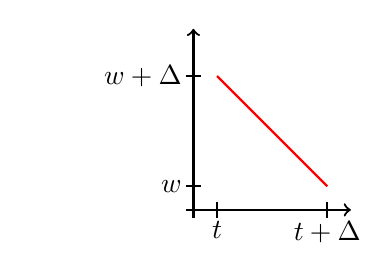
\begin{tikzpicture}[scale = 1]
\draw[->, thick] (-0.1,0) -- (2,0);
\draw[->,thick] (0,-0.1) -- (0,2.3);
\draw[-, thick] (0.3,-0.1) -- (0.3,0.1) node[inner sep=1pt,at start, anchor=north] (A)  {$t$};
\draw[-, thick] (1.7,-0.1) -- (1.7,0.1) node[inner sep=1pt,at start, anchor=north] (A)  {$t+\Delta$};
\draw[-, thick] (-.1,0.3) -- (0.1,0.3) node[inner sep=1pt,at start, left] (A)  {$w$};
\draw[-, thick] (-.1,1.7) -- (.1,1.7) node[inner sep=1pt,at start, left] (A)  {$\qquad\ \  w+\Delta$};
\draw[-, thick, color=red!100] (0.3,1.7) -- (1.7,0.3);
\end{tikzpicture}
\caption{$Q_1$ in \eqref{eq:f1}.}
\end{subfigure}
\begin{subfigure}{.45\textwidth}
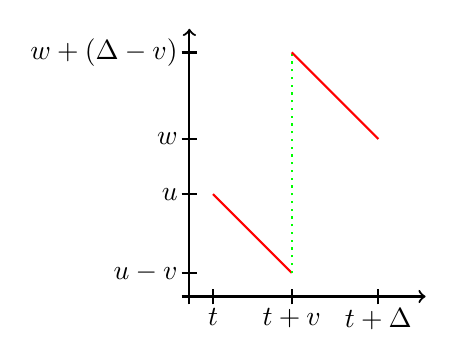
\begin{tikzpicture} [scale = 1]
\draw[->, thick] (-0.1,0) -- (3,0);
\draw[->,thick] (0,-0.1) -- (0,3.4);
\draw[-, thick] (0.3,-0.1) -- (0.3,0.1) node[inner sep=1pt,at start, anchor=north] (A)  {$t$};
\draw[-, thick] (1.3,-0.1) -- (1.3,0.1) node[inner sep=1pt,at start, anchor=north] (A)  {$t+v$};
\draw[-, thick] (2.4,-0.1) -- (2.4,0.1) node[inner sep=1pt,at start, anchor=north] (A)  {$t+\Delta$};

\draw[-, thick] (-.1,0.3) -- (0.1,0.3) node[inner sep=1pt,at start, left] (A)  {$u-v$};
\draw[-, thick] (-.1,1.3) -- (0.1,1.3) node[inner sep=1pt,at start, left] (A)  {$u$};
\draw[-, thick] (-.1,2) -- (0.1,2) node[inner sep=1pt,at start, left] (A)  {$w$};
\draw[-, thick] (-.1,3.1) -- (.1,3.1) node[inner sep=1pt,at start, left] (A)  {$w+(\Delta-v)$};
\draw[-, thick, color=red!100] (0.3,1.3) -- (1.3,0.3);
\draw[dotted, thick, color=green!100] (1.3,0.3) -- (1.3,3.1);
\draw[-, thick, color=red!100] (1.3,3.1) -- (2.4,2);
\end{tikzpicture}
\caption{$Q_2$ in \eqref{eq:f1}.}
\end{subfigure}
\begin{subfigure}{.45\textwidth}
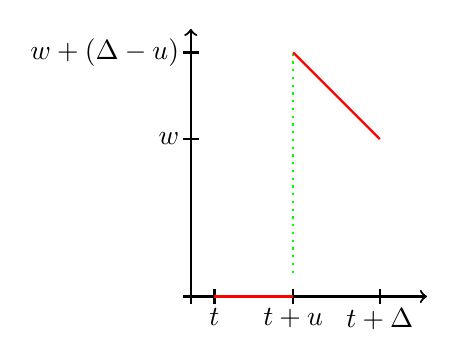
\begin{tikzpicture} [scale = 1]
\draw[->, thick] (-0.1,0) -- (3,0);
\draw[->,thick] (0,-0.1) -- (0,3.4);
\draw[-, thick] (0.3,-0.1) -- (0.3,0.1) node[inner sep=1pt,at start, anchor=north] (A)  {$t$};
\draw[-, thick] (1.3,-0.1) -- (1.3,0.1) node[inner sep=1pt,at start, anchor=north] (A)  {$t+u$};
\draw[-, thick] (2.4,-0.1) -- (2.4,0.1) node[inner sep=1pt,at start, anchor=north] (A)  {$t+\Delta$};

\draw[-, thick] (-.1,2) -- (0.1,2) node[inner sep=1pt,at start, left] (A)  {$w$};
\draw[-, thick] (-.1,3.1) -- (.1,3.1) node[inner sep=1pt,at start, left] (A)  {$w+(\Delta-u)$};
\draw[-, very thick, color=red!100] (0.3,0) -- (1.3,0);
\draw[dotted, thick, color=green!100] (1.3,0.3) -- (1.3,3.1);
\draw[-, thick, color=red!100] (1.3,3.1) -- (2.4,2);
\end{tikzpicture}
\caption{$Q_3$ in \eqref{eq:f1}.}
\end{subfigure}
\begin{subfigure}{.45\textwidth}
\begin{tikzpicture}[scale = 1]
\draw[->, thick] (-0.1,0) -- (2,0) node[inner sep=1pt,at start, anchor=east] (A) {$\qquad \qquad \qquad$};
\draw[->,thick] (0,-0.1) -- (0,2.0);
\draw[-, thick] (0.3,-0.1) -- (0.3,0.1) node[inner sep=1pt,at start, anchor=north] (A)  {$t$};
\draw[-, thick] (1.7,-0.1) -- (1.7,0.1) node[inner sep=1pt,at start, anchor=north] (A)  {$t+\Delta$};
\draw[-, very thick, color=red!100] (0.3,0) -- (1.7,0);
\end{tikzpicture}
\caption{Queue stays empty in \eqref{eq:empty_queue_thm1}.}
\end{subfigure}
\begin{subfigure}{.45\textwidth}
\begin{tikzpicture}[scale = 1]
\draw[->, thick] (-0.1,0) -- (4,0);
\draw[->,thick] (0,-0.1) -- (0,2.3);
\draw[-, thick] (0.3,-0.1) -- (0.3,0.1) node[inner sep=1pt,at start, anchor=north] (A)  {$t$};
\draw[-, thick] (2.3,-0.1) -- (2.3,0.1) node[inner sep=1pt,at start, anchor=north] (A)  {$t+u$};
\draw[-, thick] (3.7,-0.1) -- (3.7,0.1) node[inner sep=1pt,at start, anchor=north] (A)  {$t+\Delta$};
\draw[-, thick] (-.1,1.4) -- (.1,1.4) node[inner sep=1pt,at start, left] (A)  {$\qquad \quad\Delta-u$};
\draw[-, very thick, color=red!100] (2.3,1.4) -- (3.7,0);
\end{tikzpicture}
\caption{Queue becomes empty in \eqref{eq:empty_queue_thm1}}
\end{subfigure}
\caption{Graphical illustration for the proof of Theorem \ref{th:PIDE}} \label{fig:Q1Q2Q3_LLd}
\end{center}
\end{figure}
The terms $Q_i$, for $i=1,2$ and $3$ are graphically illustrated in Figure \ref{fig:Q1Q2Q3_LLd} discussed next.
\begin{enumerate}
\item[($Q_1$)] No arrivals in the interval $[t,t+\Delta]$: if the cavity queue at time $t$ has a workload exactly equal to $w + \Delta$ and experiences no arrivals 
in $[t,t+\Delta]$, it will have a workload equal to $w$ at time $t+\Delta$. The density of having a workload $w+\Delta$ at time $t$ is given by $f(t,w+\Delta)$ and the density at which an arrival occurs at the cavity queue at time $t+u, u \in [0,\Delta]$, when it has workload $w+\Delta-u$,
is equal to $\lambda d c_d(t+u, w + \Delta - u)$. Therefore we find:
$$
Q_1 = f(t, w + \Delta) - \lambda d \int_{u=0}^{\Delta} c_d(t+u,w+\Delta - u) du.
$$
\item[($Q_2$)]A single arrival occurs when the cavity queue is not idle: in this case at some time $t+v, v \in [0,\Delta]$ an arrival of size $w+\Delta-v$ occurs at 
the cavity queue which has workload $u-v$ for some $u \in [v,w+\Delta]$ occurs. We find:
$$
Q_2 = \lambda d  \int_{v=0}^{\Delta} \int_{u=v}^{w+\Delta} c_d(t+v, u-v) g(w-u+\Delta-v)dudv.
$$
\item[($Q_3$)] A single arrival occurs when the cavity queue is empty: in this case a job 
of size $w + \Delta - u$ arrives at time $t+u$ for some $u \in [0,\Delta]$. Hence,
$$
Q_3 = \lambda d \int_{u=0}^{\Delta} C_d(t+u, 0) g(w+\Delta-u)du.
$$
\end{enumerate}
By subtracting $f(t,w+\Delta)$, dividing by $\Delta$ and letting  $\Delta$ decrease to zero, we find \eqref{eq:PIDE} from \eqref{eq:f1}.

We still require a differential equation for $F(t,0)$, a server may be idle at time $t+\Delta$ by remaining idle in $[t,t+\Delta]$ or having a workload equal to $\Delta - u, u < \Delta$ at time $t + u$. We therefore find:
\begin{align}
F(t+\Delta, 0) &= F(t,0) - \lambda d \int_{u = 0}^{\Delta}C_d(t+u,0)du\\
& + \int_{u=0}^{\Delta} f(t+u, \Delta - u) du + o(\Delta), \label{eq:empty_queue_thm1}
\end{align}
subtracting $F(t,0)$, dividing by $\Delta$ and letting $\Delta$ tend to zero yields \eqref{eq:ODEF0}.
\end{proof}

\begin{remark}
The PIDE given by (\ref{eq:PIDE}-\ref{eq:ODEF0}) can be solved numerically using the following scheme:
\begin{align*}
f(t+\Delta,0^+) &=
\lambda d C_d(t,0),\\
f(t+\Delta,w) &=
f(t,w+\Delta) + \lambda d \Delta \int_0^w c_d(t,u) g(w-u) du \\
&  + \lambda d \Delta  C_d(t,0) g(w) - \lambda d \Delta  c_d(t,w),
\end{align*}
for $w \geq \Delta$. As a boundary condition, we may impose that we start with all servers being idle, 
i.e., for $w>0$ we set $f(0,w) = 0$ and $F(0,0) = 1$.
The main objective of Theorem \ref{th:PIDE} is however to use it to characterize the unique equilibrium 
environment  $\mathcal{H}$ of the LL($d$) policy.
\end{remark}

\begin{remark}
A propagation of chaos result was established in \cite[Section 7]{bramson2012asymptotic} (and more recently also in \cite{shneer2020large}) which
states that the workload distributions of any set of $N' \leq N$ queues 
at time $t$ become asymptotically independent, provided
that the workload distribution at time $0$ in the $N$ queues is i.i.d.~and does not depend on $N$, e.g., if the system is empty at time zero. As such Theorem \ref{th:PIDE} characterizes the limiting transient behavior.
\end{remark}

\section{Limiting workload distribution}\label{sec:workload}
As indicated in the previous section, the limiting stationary workload distribution is given by the unique equilibrium environment. Let $F(w)$ be the cdf of the workload distribution, that is, $F(w)$ represents the probability that the workload is at most
$w$, let $f(w)$ be its density for $w > 0$ and denote its ccdf by $\bar F(w) = 1-F(w)$. 
Furthermore, similar to \eqref{eq:C} and \eqref{eq:barC}, define:
\begin{align}
c_d(u) =  f(u)\bar{F}(u)^{d-1},
\end{align}
and
\begin{align}
C_d(u) = \frac{1 - \bar F(u)^d}{d}.
\end{align}

\begin{theorem} \label{thm:LLd_workload_gen_sizes}
The stationary workload distribution is the unique distribution for which the ccdf obeys the following FPE:
\begin{equation}\label{eq:F(s)}
\bar F(w) = \rho - \lambda \cdot \left(
\int_{0}^w (1 - \bar{F}(u)^d) \bar G(w-u) du
\right)
\end{equation}
\end{theorem}
\begin{proof}
By demanding that the derivatives with respect to $t$ are zero in (\ref{eq:PIDE}-\ref{eq:ODEF0}), we find
\begin{align}\label{eq:PIDElim}
\frac{\partial f(w)}{\partial w}&=\lambda d \left(c_d(w) - \int_{0}^{w}c_d(u)\,g(w-u)\,du -C_d(0)\,g(w)\right),
\end{align}
and
\begin{align}\label{eq:PIDElim2}
f(0^+) = \lambda d C_d(0).
\end{align}
Integrating \eqref{eq:PIDElim} once (and relying on the assumption that $G(0) = 0$) we find:
\begin{align}
f(w)
=
K-\lambda d \cdot \left( \frac{1}{d}-C_d(w) + C_d(0) G(w) + \int_0^w c_d(u) G(w-u) du \right),
\end{align}
for an appropriate constant $K$. As we know from \eqref{eq:PIDElim2} that $f(0^+) = \lambda d C_d(0)$, we see that we should set $K$ equal to $\lambda$. We may therefore conclude that
\begin{equation}\label{eq:f(s)}
f(w) =
\lambda d \cdot
\left(
C_d(w) - C_d(0) G(w) - \int_0^w c_d(u) G(w-u) du
\right)
\end{equation}
Integrating equation \eqref{eq:f(s)} once more and using the fact that $F(0) = 1-\rho$, yields
\begin{align*}
F(w) = (1-\rho) + \lambda d  \cdot \left(
\int_{0}^w C_d(u) (1 - G(w-u)) du
\right),
\end{align*}
from wich \eqref{eq:F(s)} easily follows.
The uniqueness follows from the fact that there exists a unique equilibrium environment for the LL($d$) supermarket model
as stated earlier.
\end{proof}

\begin{remark}
For $d$ large, we have $\bar{F}(u)^d \approx 0$ and therefore \eqref{eq:F(s)} yields
\[ \bar F(w) \approx \rho - \lambda \int_{0}^w \bar G(u) du = \lambda \int_w^\infty \bar G(u) \, du ,\]
meaning $f(w) \approx \lambda \bar G(w)$. Note that $\lambda \int_{0}^w \bar G(u) du$ 
can be recognized as the equilibrium distribution of the forward recurrence time of a renewal
process with inter-arrival time distribution $G$.
\end{remark}

\begin{remark}
The cavity process evolves as the workload of an M/G/1 queue with a workload dependent arrival rate, we can therefore also
apply Theorem 2.1 in \cite{bekker2004} to the LL($d$) cavity process. In this manner we obtain that
$$
f(w) = \lambda d \left( C_d(0) \bar G(w) + \int_0^w c_d(u) \bar G(w-u) du \right),
$$
which can easily be shown to be equivalent to \eqref{eq:f(s)} by using the fact that $c_d(u) = \frac{d}{du} C_d(u)$. 
The interpretation of this equation is as follows. The left-hand side of the equation corresponds to the downcrossing rate through level $w$, while the right-hand side denotes the upcrossing rate through $w$. Another way to write this equality is :
\begin{equation}\label{eq:IDE_LLd1}
\bar F'(w) = -\lambda \bigg[ \int_0^w \bar F(u)^d g(w-u) \, du + \bar G(w) - \bar F(w)^d \bigg].
\end{equation}
This equation is not all too important for LL($d$) but in the upcoming chapters, it is this equation which we generalize to other workload dependent load balancing policies.
\end{remark}

\subsection{Fixed point iteration}\label{sec:fixed}
We propose to use the following simple FPI to solve the integral equation
\eqref{eq:F(s)}:
\[\bar F_{n+1}(w) = \rho - \lambda \cdot \left(
\int_{0}^w (1 - \bar{F}_n(u)^d) \bar G(w-u) du
\right),\]
which we prove converges to the unique fixed point provided that $\rho < d^{-1/d}$.
In Section \ref{sec:ph} we further show that if the job sizes follow a PH
distribution, we can directly compute the limiting workload distribution $\bar F(w)$ by solving a 
simple set of ODEs (for any $\rho < 1$), meaning there is no need to 
make use of the above FPI. Furthermore, the DIDE given in \eqref{eq:IDE_LLd1} can alternatively be used to obtain $\bar F(w)$.

Define the function space $\operatorname{ccdf}_{\rho} \subseteq [0, \rho]^{[0,\infty)}$ to be the space of complemented cumulative distribution functions starting in $\rho$, i.e., the space of functions which satisfy: 
\begin{itemize}
\item $\bar F(0) = \rho$,
\item $\lim_{w\rightarrow\infty} \bar F(w) = 0$,
\item for $w,h>0: \bar F(w+h) \leq \bar F(w)$,
\item for $w>0: \lim_{h\rightarrow 0^+} \bar F(w+h) = \bar F(w)$.
\end{itemize}
On this space we can define an operator $T_d: \operatorname{ccdf}_{\rho} \longrightarrow \R^{[0,\infty)}$ defined by:
$$
T_d\bar F: [0,\infty) \rightarrow \R: w \mapsto \rho - \lambda \cdot \left( \int_{0}^w (1-\bar F(u)^d) \bar G(w-u) du \right).
$$
\begin{lemma}\label{operator_lem}
For $\bar F \in \operatorname{ccdf}_{\rho}$, we have $T_d\bar F \in \operatorname{ccdf}_{\rho}$.
\end{lemma}\begin{proof}
The only non-trivial part is to show that $\lim_{w\rightarrow \infty} T_d\bar F(w) = 0$. We find:
\begin{align*}
\lim_{w\rightarrow \infty} \left| \int_0^w (1-\bar F(u)^d) \cdot \bar G(w-u) du \right|
&\leq \lim_{w\rightarrow \infty} \int_0^w \bar G(w-u) du\\
&= \E[G],
\end{align*}
which shows that $\lim_{w\rightarrow \infty} T_d\bar F(w) \geq 0$. To obtain the other inequality observe that for any $\varepsilon > 0$, we can find a $U > 0$ for which:
\begin{align*}
&\lim_{w\rightarrow \infty} \int_U^w \bar G(w-u) du > \sqrt{1 - \varepsilon} \E[G],
&1-\bar F(u)^d \geq \sqrt{1 - \varepsilon},
\end{align*}
for $u > U$.
We thus find:
\begin{align*}
\lim_{w\rightarrow \infty} \int_0^w d (1-\bar F(u)^d) \bar G(w-u)\, du
& \geq \lim_{w\rightarrow \infty} \int_U^w d (1-\bar F(u)^d) \bar G(w-u)\, du\\
& \geq (1 - \varepsilon)\E[G]
\end{align*}
this shows that $\lim_{w\rightarrow\infty}T_d\bar F(w) \leq 0$
\end{proof}

\begin{remark}
Due to the above lemma we may write $T_d: \operatorname{ccdf}_{\rho} \rightarrow \operatorname{ccdf}_{\rho}$.
\end{remark}
\begin{remark}
We can define an order on $\mbox{ccdf}_{\rho}$ by stating that $\bar F_1 \preceq \bar F_2 \Leftrightarrow \forall w \in [0,\infty): \bar F_1(w) \geq \bar F_2(w)$, then a simple application of the Knaster-Tarski theorem \cite{tarski1955} guarantees the existence of a fixed point of $T_d$. Indeed note that we have $\bar F_1 \preceq \bar F_2 \Rightarrow T_d \bar F_1 \preceq T_d \bar F_2$.
\end{remark}

\begin{theorem}\label{operator_eig}
For any $\bar F_1,\bar F_2 \in \operatorname{ccdf}_{\rho}$ we have:
$$
d_K(T_d\bar F_1,T_d\bar F_2) \leq d \rho^d \cdot d_K(\bar F_1, \bar F_2),
$$
where $d_K$ denotes the uniform (or Kolmogorov) metric, i.e.,
$d_K(\bar F_1, \bar F_2) = \sup_w |\bar F_1(w)-\bar F_2(w)|$.
\end{theorem}
\begin{proof}
Let $\varepsilon > 0$ be arbitrary and let $w^*$ be such that:
\begin{align*}
&\sup_w \int_0^w |\bar F_1(u)^d - \bar F_2(u)^d| \bar G(w-u)\, du\\
&<
\int_0^{w^*} |\bar F_1(u)^d -  \bar F_2(u)^d| \bar G(w^*-u))\, du + \varepsilon.
\end{align*}
We therefore have that $d_K(T_d\bar F_1,T_d\bar F_2)$ is bounded above by:
\begin{align*}
\lambda \int_0^{w^*} |\bar F_2(u)^d - \bar F_1(u)^d| \bar G(w^*-u)\, du + \varepsilon.
\end{align*}
We now use the fact (which can be shown by applying the mean value theorem) that for any $x,y \in [0,\rho)$
we have $|x^d - y^d| \leq d  \rho^{d-1} \cdot |x-y|$. This shows by applying the above that we have:
\begin{align*}
d_K(T_d\bar F_1,T_d\bar F_2)
&
< \lambda \int_0^{w^*} d \rho^{d-1} |\bar F_1(u) - \bar F_2(u)| \bar G(w^*-u)\, du + \varepsilon\\
&
\leq \lambda d \rho^{d-1} d_K(\bar F_1,\bar F_2) \int_0^{w^*} \bar G(w^*-u)\, du + \varepsilon\\
&\leq d \rho^{d} d_K(\bar F_1,\bar F_2) + \varepsilon,
\end{align*}
which completes the proof.
\end{proof}

\begin{remark}
In particular, for $\rho < e^{-1/e} \approx 0.6922$ the above theorem shows by the Banach fixed-point theorem that $T_d$ admits a unique fixed point which can be found by our proposed FPI with speed of convergence $d_K(\bar F^*, \bar F_n) \leq \frac{d^n \rho^{nd}}{1 - d \rho^d} d_K(\bar F_1,\bar F_0)$. 
This follows from the fact that $d^{-1/d}$ attains a minimum in $e$. For higher values of 
$\rho$, $d$ must be such that $d \rho^d < 1$ to guarantee convergence via Theorem \ref{operator_eig}.
Numerical experiments using both light-tailed and heavy-tailed distributions suggest that the FPI converges quickly for any $\rho < 1$. 
\end{remark}
\begin{remark}
Alternatively, one can solve the DIDE given in \eqref{eq:IDE_LLd1}. Both methods are fast and appear to work for values of $\rho$ close to one. Moreover, we will see in Chapter \ref{chap:workload_dependent} that for more complex models, solving \eqref{eq:IDE_LLd1} is more efficient whenever a forward Euler scheme can be used (this is the case for future independent models). When the DIDE can not be solved using a forward Euler scheme, solving the FPE using a FPI proves to be more efficient (as is the case for future dependent models).
\end{remark}

Using this numerical method, we can also compute the waiting and response time distribution. Indeed, the ccdf of the waiting time is given by $\bar F_W(w)=\bar F(w)^d$. The ccdf of the response time is given by the convolution of $g$ with the ccdf of the waiting time, i.e.~$\bar F_R(w) = \bar G(w) + (g * \bar F_W)(w)$.


\section{Exponential job sizes}\label{sec:expo}
In the previous section we established an integral equation for the limiting stationary workload
distribution (for any non-idling service discipline). In this section we derive an explicit
expression for this distribution in case of exponential job sizes with mean $1$, that is, when $\bar G(w) =  e^{-w}$
and $\rho = \lambda$.
In addition we also derive an explicit expression for the limiting response time distribution in case
the service discipline is FCFS. Assuming $\E[G]=1$ is only for technical reasons, to obtain the results for the case where $\E[G]$ is arbitrary, one mostly needs to replace occurrences of $\lambda$ by $\rho$.

\subsection{Limiting workload distribution}
\begin{theorem} \label{thm:LLd_exp}
The ccdf of the limiting stationary workload distribution for the LL($d$) policy for any non-idling 
service discipline with exponential job sizes with mean $1$ is given by:
\begin{equation}\label{eq:expExact}
\bar{F}(w) = (\lambda + (\lambda ^{1-d} - \lambda) e^{(d-1)w})^{\frac{1}{1-d}}.
\end{equation}
\end{theorem}
\begin{proof}
Using \eqref{eq:F(s)} with $\bar G(w) = e^{-w}$
and $\rho = \lambda$, we have
\begin{equation}\label{eq:F(s)exponential}
\bar F(w) = \lambda - \lambda d \int_{0}^w C_d(u) e^{u-w} du,
\end{equation}
Taking the derivative on both sides and using the Leibniz integral rule, we find the following simple ODE for $\bar F(w)$:
\begin{align}\label{eq:ODEexp}
\bar F'(w) &= -\lambda (1-\bar{F}(w)^d) +\lambda \int_{0}^w (1-\bar{F}(u)^d)e^{u-w}du \nonumber\\
&= -\lambda (1-\bar{F}(w)^d) + (F(w)-(1-\lambda)) \nonumber \\
&= - \bar{F}(w) + \lambda \bar{F}(w)^d,
\end{align}
with boundary condition $\bar F(0) = \lambda$. This ODE can be solved explicitly and one easily verifies that the solution $\bar{F}(w)$ is given by:
$$
\bar{F}(w) = (\lambda + (\lambda ^{1-d} - \lambda) e^{(d-1)w})^{\frac{1}{1-d}}.
$$
\end{proof}


\begin{remark}
There is a striking and unexpected similarity between the limiting workload distribution of the LL($d$) policy
and the response time distribution of the replication with cancellation on completion \cite[Section 5]{gardnerOR} in case of exponential
job sizes in the sense that the response time distribution of the latter system solves exactly
the same ODE as in \eqref{eq:ODEexp}, except that it is subject to the boundary condition $\bar{F}_R(0) = 1$, with $\bar{F}_R$ the response time distribution for replication, with cancellation on completion and i.i.d.~replicas (see also \eqref{prop:gardner}).
\end{remark}


\begin{remark}
For $d$ large, $\bar{F}(w)$ can be approximated by $\lambda e^{-w}$
as $(\lambda^{1-d} - \lambda) ^{1/(1-d)}$ is close to $\lambda$ for large $d$.
This result is expected as for large $d$ we expect that a fraction $\lambda$ of the
servers contains exactly one job and the remaining workload of any such job is
exponentially distributed due to the memoryless nature of the exponential distribution.
\end{remark}

In order to obtain an expression for the expected workload of a server, we first recall the following 
integral representation for the analytic continuation of the hypergeometric function $\prescript{}{2}{F}_1(a,b;c;z)$ 
\cite[Chapter 15]{abramowitz64}
\begin{align}\label{eq:int2F1}
\prescript{}{2}{F}_1(a,b;c;z) = \frac{1}{B(b,c-b)} \int_{0}^1 x^{b-1} (1-x)^{c-b-1} (1-zx)^{-a} dx,
\end{align}
where $B(x,y) = \int_0^1 t^{x-1} (1-t)^{y-1} dt$ is the Beta function. 
This integral expression is valid for any $c > b > 0$ and $z < 1$. When $|z| < 1$ this function can be represented
as an infinite sum using the Pochhammer symbol (or falling factorial) $(q)_n = \prod_{k=0}^{n-1} (q+k)$ when
$n > 0$ and $(q)_0 = 1$: 
\begin{align}\label{eq:sum2F1}
\prescript{}{2}{F}_1(a,b;c;z) = \sum_{n=0}^\infty \frac{(a)_n(b)_n}{(c)_n} \frac{z^n}{n!}.
\end{align}

\begin{theorem}\label{th:Wd}
The mean workload $\E[L_d]$ under the LL($d$) policy with exponential job sizes with mean $1$
is given by:
\begin{equation}\label{W_d}
\E[L_d] = \sum_{n=0}^{\infty} \frac{\lambda^{dn+1}}{1 + n(d-1)},
\end{equation}
in particular we find:
\begin{align*}
\E[L_2] &= - \frac{\log\left( 1 - \lambda ^ 2 \right)}{\lambda},\\
\E[L_3] &= - \frac{1}{\sqrt{\lambda}} \cdot \log\left( \frac{\sqrt{1 - \lambda^3}}{\lambda^{3/2} + 1} \right).
\end{align*}
\end{theorem}
\begin{proof}
We employ the notation $b = \lambda^{1-d} - \lambda$. 
We begin by computing (using $y=e^{-w}$ and $x=y^{d-1}$):
\begin{align*}
\E[L_d] &= \int_0^\infty \bar{F}(w)dw\\
&=  \int_0^1 \frac{1}{(\lambda y^{d-1} + b)^{1/(d-1)}} dy\\
&=  \frac{1}{b^{1/(d-1)}} \frac{1}{(d-1)} \int_0^1 \frac{x^{-(d-2)/(d-1)}}{(1+\frac{\lambda}{b} x)^{1/(d-1)}} dx
%&= \frac{1}{\lambda^{1/(d-1)}} \int_0^{(\lambda/b)^{1/(d-1)}} \frac{1}{(1 + x^{d-1})^{1/(d-1)}} dx.
\end{align*}
Hence, by \eqref{eq:int2F1} this last integral can be expressed via the hypergeometric function $\prescript{}{2}{F}_1$ as 
$$
\E[L_d] = \frac{1}{b^{1/(d-1)}}\cdot \prescript{}{2}{F}_1\left( \frac{1}{d-1}, \frac{1}{d-1}; 1 + \frac{1}{d-1}; -\frac{\lambda}{b}\right).
$$
Note that we cannot directly use the sum representation of $_2F_1$ as $\lambda / b$ may become greater than $1$ (which happens when 
$\lambda$ gets close to one). Therefore we now employ the well-known linear transformation formulas:
\begin{align}
\prescript{}{2}{F}_1(a,b;c;z) & = (1-z)^{c-a-b} \cdot  \prescript{}{2}{F}_1(c-a, c-b; c; z) \nonumber\\
\prescript{}{2}{F}_1(a,b;c;z) & = (1-z)^{-a} \cdot  \prescript{}{2}{F}_1\left(a,c-b;c;\frac{z}{z-1}\right).
\label{eq:lintrans2}
\end{align}
Using \eqref{eq:lintrans2} indicates that
\begin{align*}
\E[L_d] & = \frac{1}{b^{1/(d-1)}} \left(1+\frac{\lambda}{b}  \right)^{-\frac{1}{d-1}} \cdot  \prescript{}{2}{F}_1\left( 1,\frac{1}{d-1};1+\frac{1}{d-1};\lambda^d \right) \\
& = \lambda \cdot \prescript{}{2}{F}_1\left( 1,\frac{1}{d-1};1+\frac{1}{d-1};\lambda^d \right) 
\end{align*}
As $\lambda^d \in (0,1)$, we can use the sum representation given by \eqref{eq:sum2F1} to find that
$$
\E[L_d] =\sum_{n=0}^{\infty} \frac{\lambda^{nd+1}}{1 + n (d-1)},
$$
as $(1)_n = n!$ and $(1/(d-1))_n/(1/(d-1)+1)_n = 1/(1+n(d-1))$.
The expressions for $d=2,3$ can be either found directly by looking at the Taylor expansion of the logarithm or by solving the integral representation of $\E[L_d]$.
\end{proof}



\subsection{Limiting waiting and response time distribution}
We now focus on the limiting waiting and response time distribution $W$ and $R$ in case the service discipline is FCFS. For the ccdf of the waiting time distribution, one easily finds that it is given by $\bar F_W(w) = \bar F(w)^d$. For the ccdf of the response time distribution, we find:

\begin{theorem}
The ccdf of the limiting response time distribution of the LL($d$) policy with
FCFS service and exponential job sizes with mean $1$ is given by:
\begin{equation}\label{eq:FR}
\bar{F}_R(w) = \left( \lambda^d + (1 -\lambda^d) e^{(d-1)w} \right)^{\frac{1}{1-d}}.
\end{equation}
\end{theorem}
\begin{proof}
Let $E$ be an exponential random variable with mean $1$ and let $L_i,i = 1,\dots, d$ denote the $d$ independent workloads of the
$d$ randomly selected servers. We find:
\begin{align*}
\bar{F}_R(w)
&= \P\left\{E + \min_{i=1}^d L_i > w\right\}\\
%&= \int_{0}^{\infty} \P\left\{\min_{i=1}^d T_i > w - t\right\} e^{-t} dt\\
%&= \int_{0}^w \P\left\{\min_{i=1}^d T_i > w - t\right\} e^{-t} dt + \int_w^{\infty} e^{-t} dt\\
&= e^{-w} + \int_0^{w} \bar{F}(w-t)^d e^{-t} dt.
\end{align*}
Due to \eqref{eq:expExact} and using standard integration techniques, this integral can be simplified to:
$$
\bar{F}_R(w) = e^{-w} \cdot \left(1 + \frac{1}{\lambda b^{1/(d-1)}} \cdot \int_{\left(\frac{b}{\lambda}\right)^{1/(d-1)}}^{e^w \left(\frac{b}{\lambda}\right)^{1/(d-1)} } (1 + x^{d-1})^{d/(1-d)} dx \right),
$$
where $b= \lambda^{1-d} - \lambda$ as before.
This is an integral that can be solved exactly to prove the statement. 
\end{proof}

\begin{remark}
It is easy to verify that the workload and response time distributions $\bar F(w)$ and $\bar F_R(w)$ have 
the same increasing failure rate $r(w) = f(w)/\bar{F}(w) = f_R(w)/\bar{F}_R(w)$.
\end{remark}
%\begin{proof}
%One can show that $r_R(s) = r(s)$ and therefore the result follows from Proposition \ref{prop:fr}.
%\end{proof}

\begin{remark}
For $d$ large, $\bar F_R(w) \approx e^{-w}$, as expected. 
\end{remark}

\begin{theorem}\label{eig:T_d}
The mean of the limiting response time distribution for the LL($d$) policy with FCFS service
and exponential job sizes with mean $1$ is given by:
\begin{equation}\label{eq:T_kclosed}
\E[R]
=
\sum_{n=0}^{\infty} \frac{\lambda^{dn}}{1 + n \cdot (d-1)}.
\end{equation}
\end{theorem}
The mean waiting time is given by $\E[W] = \E[R] - 1 = \sum_{n=1}^{\infty} \frac{\lambda^{dn}}{1 + n \cdot (d-1)}$.
\begin{proof}
Let $L_i$ be i.i.d.~copies of the workload distribution $L$ and $E$ an exponential distribution with mean one, we find:
\begin{align*}
\E[R] &= \E[E + \min\{L_1,\dots,L_d\}]\\
%&= 1 + \E[\min\{L_1,\dots,L_d\}]\\
&=1 + \int_0^\infty \bar{F}(w)^dds.
\end{align*}
Using \eqref{eq:expExact} and standard integration techniques (mainly substitution), we can reduce this expression to:
$$
\E[R] = 1 + \frac{1}{\lambda^{d/(d-1)} \cdot (d-1)} \cdot \int_0^{\lambda / b} \frac{v^{1/(d-1)}}{(1+v)^{d/(d-1)}} dv.
$$
Using the substitution $y = \frac{v}{1 + v}$, one can show that the above integral reduces to
$$
1 + \frac{\lambda^d}{d} \cdot \prescript{}{2}F_1 \left( \frac{d}{d-1},1;1+\frac{d}{d-1};\lambda^d\right).
$$
As $\lambda^d \in (0,1)$, one can use \eqref{eq:sum2F1} and the claimed equality follows as $(1)_n=n!$ and $(d/(d-1))_n/(1+d/(d-1))_n = d/((n+1)(d-1)+1)$. 
\end{proof}

\begin{remark}
In the proof of Theorem \ref{eig:T_d} it is also possible to directly use \eqref{eq:FR} instead of relying on \eqref{eq:expExact}.
\end{remark}

\begin{remark}
Note that by combining Theorems \ref{th:Wd} and \ref{eig:T_d} we have shown that $\E[L] = \lambda \E[R]$. Due to Little's law this shows that the mean workload of a server under the LL($d$) policy for exponential job sizes with mean $1$ is equal to the mean number
of jobs in such a server, that is $\E[L]=\E[Q]$. 
The relation $\E[L] = \lambda \E[R]$ also yields simple formulas for 
$\E[R]$ in case $d=2,3$ due to Theorem \ref{th:Wd}. It is possible to derive similar expressions for larger $d$ values, but these become more and more complex as $d$ increases. 
\end{remark}


\begin{remark}
In \cite{gardnerOR} the mean of the limiting response time distribution
in case of exponential job sizes for the replication with cancellation on completion policy (under the {\it assumption} of the independence ansatz) was argued to be equal to (with $\mu = 1/\E[G]$):
$$
\E[R^{Red_{\text{iid}}(d)}] = \frac{\prescript{}{2}F_1(1,1;1+\frac{d}{d-1};\frac{-\rho}{1-\rho})}{\mu d(1-\rho)}.
$$
This expression can be reduced to a simple sum formula as follows (using \eqref{eq:lintrans2} and \eqref{eq:sum2F1} as $\rho \in (0,1)$) 
\begin{align*}
\prescript{}{2}F_1\left(1,1;1+\frac{d}{d-1};\frac{-\rho}{1-\rho}\right)
&= (1-\rho) \prescript{}{2}F_1(1,\frac{d}{d-1};1+\frac{d}{d-1};\rho)\\
&= (1-\rho) \sum_{n=0}^{\infty} \frac{(1)_n \left( \frac{d}{d-1}\right)_n}{\left(1+\frac{d}{d-1}\right)_n} \frac{\rho^n}{n!},
\end{align*}
which allows us to conclude that
\[\E[R^{Red_{\text{iid}}(d)}] = \frac{1}{\mu} \sum_{n=0}^\infty \frac{\rho^n}{n(d-1)+d}.
\]
Note that $E[R^{Red_{\text{iid}}(d)}]$ converges to $1/(d\mu)$ as $\rho$ tends to zero due to the independent execution times of the replicas in \cite{gardnerOR}.
\end{remark}

\section{Phase-type and deterministic job sizes}\label{sec:ph}

In Section \ref{sec:fixed} we proposed a FPI to compute the limiting workload distribution $\bar F(w)$ under LL($d$) 
for any job size distribution $\bar G$, that was proven to converge if
$d \rho^d < 1$. We now show that $\bar F(w)$ can also be directly obtained as the solution of a set of coupled ODEs for any $\rho < 1$, provided that the job lengths follow a PH distribution. 
PH distributions are distributions with a modulating finite state background Markov chain \cite{latouche1} and any general positive-valued distribution 
can be approximated arbitrary closely with a PH distributions. Further, various fitting tools are available online 
for PH distributions (e.g., \cite{panchenko1,Kriege2014}). 
A PH distribution with $G(0)=0$ is fully characterized by a stochastic vector $\alpha = (\alpha_i)_{i=1}^n$ and a subgenerator matrix  $A = (a_{i,j})_{i,j=1}^n$
such that $\bar G(w) = \alpha e^{Aw} \textbf{1}$, where $\textbf{1}$ is a column vector of ones.
 
\begin{theorem}\label{eig:PHD}
Suppose the job lengths have a PH distribution characterized by $(\alpha,A)$, then the ccdf of the 
limiting workload distribution under the LL($d$) policy satisfies:
\begin{align*}
\bar{F}'(w) & = -\lambda \left((1-\bar{F}(w)^d\right) + \alpha A \xi(w)),\\
\xi'(w) & = \left(1-\bar{F}(w)^d\right) \textbf{1} + A \xi(w),
\end{align*}
with $\bar{F}(0) = \rho$, $\xi(0) = 0$ and
$\xi(w): \R \rightarrow \R^{n \times 1}$.
\end{theorem}
\begin{proof}
For $i \in \{1,\dots,n\}$ we define:
$$
\xi_{i}(w) = \int_0^w (1-\bar{F}(u)^d) e_i^T e^{(w-u)A} \textbf{1} du,
$$
where $e^T_i$ is the $i$-th row of the identity matrix $I_n$.
First note that $\xi_{i}(0) = 0$. We now derive a differential equation for $\xi_{i}(w)$. 
Using the equality $I_n = \sum_{k=1}^n e_k e_k^T$ we find :
\begin{align*}
\xi_{i}'(w)
&= (1-\bar{F}(w)^d) + \int_0^w (1 - \bar{F}(u)^d) e_i^T A I_n e^{(w-u)A} \textbf{1} du\\
&= (1-\bar{F}(w)^d) + \sum_{k=1}^n \int_0^w (1-\bar{F}(u)^d) e_i^T A e_k e_k^T e^{(w-u)A}\textbf{1} du \\
&= (1-\bar{F}(w)^d) + \sum_{k=1}^n a_{i,k} \xi_{k}(w).
\end{align*}
In matrix notation this yields:
$$
\xi'(w) = (1-\bar{F}(w)^d) \textbf{1} + A \xi(w).
$$
Due to \eqref{eq:F(s)} and $\bar G(w-u) = \alpha e^{(w-u)A} \textbf{1}$, 
we have $\bar{F}'(w) = -\lambda \alpha \xi'(w)$, which yields the equation for $\bar{F}'(w)$.
\end{proof}
\begin{remark}
We could have alternatively derived the result of Theorem \ref{eig:PHD} directly from \eqref{eq:IDE_LLd1}. Indeed, we have $g(w)=\alpha e^{Aw} \mu$ with $\mu=-A\cdot \textbf{1}$, using \eqref{eq:IDE_LLd1}, we obtain:
\begin{equation} \label{eq:IDE_LLd_expo}
\bar F'(w) = -\lambda\bigg[
(1-\bar F(w)^d) - \alpha \int_0^w (1-\bar F(u)^d) e^{(w-u) A} \mu \, du
\bigg].
\end{equation}
Defining $\xi(w)=\int_0^w (1 - \bar F(u)^d) e^{(w-u)A} \mu \, du$ as in the above proof, one may recover the result directly from \eqref{eq:IDE_LLd_expo}.
This method generalizes well to other workload dependent load balancing policies and is further explored in Section \ref{sec:PH_dist}.
\end{remark}

We now generalize this result to the case where the service times 
are the sum of a deterministic random variable and a PH distribution.

\begin{theorem}\label{th:X+PH}
Assume the service times are the sum of a deterministic random variable equal to $\tau > 0$ and
a phase-type distribution characterized by $(\alpha,A)$,
i.e., $\bar{G}(w) = I_{\{w\leq \tau\}} + I_{\{w > \tau\}} \alpha e^{(w-\tau) A} \textbf{1}$,
then the ccdf of the limiting workload distribution under the LL($d$) policy satisfies:
\begin{align*}
\bar{F}'(w) &= -\lambda(1-\bar{F}(w)^d), & w \leq \tau,\\
\bar{F}'(w) &= -\lambda((1 - \bar{F}(w)^d) +\alpha A \xi(w-\tau)), & w > \tau,\\
\xi'(w) & = (1-\bar{F}(w)^d) \textbf{1} + A \xi(w),
\end{align*}
with $\xi(0) = 0$ and $\bar{F}(0) = \rho = \lambda (\tau + \alpha(-A)^{-1}\textbf{1})$.
\end{theorem}
\begin{proof}
We distinguish two cases: first let $w \in [0,\tau]$, we find that $\bar{F}(w) = \rho - \lambda \int_0^w 1 - \bar{F}(u)^d du$, differentiating this equation once yields the first equation.

For the second note that we have (using the notation from the proof of Theorem \ref{eig:PHD}):
$$
\bar{F}(w) = \rho - \lambda \alpha \xi(w-\tau)  - \lambda \int_{w-\tau}^w (1-\bar{F}(u)^d) du.
$$
Taking the derivative and using the expression for $\xi'(w)$ found in Theorem \ref{eig:PHD} completes the proof.
\end{proof}
From the above result, we obtain a very simple DDE for $\bar F(w)$ in case job sizes are deterministic.

\begin{theorem}\label{thm:det}
If the job sizes are deterministic and equal to one, the ccdf $\bar{F}(w)$ is determined by $\bar{F}(0)=\lambda$, 
and
\begin{align*}
\bar{F}'(w) &= - \lambda (1-\bar{F}(w)^d) & w \in [0,1),\\
\bar{F}'(w) &= - \lambda (\bar{F}(w-1)^d - \bar{F}(w)^d) & w \geq 1.
\end{align*}
\end{theorem}
\begin{proof}
The proof is similar to the proof of Theorem \ref{th:X+PH}.
\end{proof}
In general, when job sizes have a discrete distribution $\sum_n p_n \delta_{x_n}$ and we assume without loss of generality that $x_0 < x_1 < \dots$, it is not hard to see that the result of Theorem \ref{thm:det} generalizes to:
\begin{align*}
\bar F'(w) &= -\lambda (1-\bar F(w)^d) & w \in [0,x_0),\\
\bar F'(w) &= -\lambda (p_0 \bar F(w-x_0)^d - \bar F(w)^d) & w \in [x_0, x_1),\\
\bar F'(w) &= -\lambda ( p_0 \bar F(w-x_0)^d + p_1 \bar F(w-x_1)^d - \bar F(w)^d) & w \in [x_1,x_2),\\
\dots
\end{align*}
Combining this result with Theorem \ref{eig:PHD} allows one to reduce the computation of $\bar F(w)$ in case the job size distribution is a mix of a discrete distribution and a PH distribution to solving a system of DDEs.
\begin{remark}
We note that the ODEs and DDEs presented in this section have a unique solution: the existence follows from the fact that \eqref{eq:F(s)} solves the ODE/DDE, 
while the uniqueness follows from \cite[Section 23, theorem A]{driver1977}.
\end{remark}

\begin{remark}
It is easy to compute the ccdf of the waiting and response time distribution $\bar{F}_R(w)$ given $\bar{F}(w)$ as
the probability that a new arrival joins a queue with a workload exceeding $w$ is given by $\bar F_W(w) = \bar{F}(w)^d$
under the LL($d$) policy. Furthermore, the response time is simply the convolution of the job size distribution and the waiting time distribution as these are independent random variables.
\end{remark}


\section{LL($d$) versus SQ($d$)}\label{sec:versus}

The aim of this section is to study the margin of improvement that can be achieved by using 
exact workload information as opposed to the coarser queue length information used
by SQ($d$). This margin of improvement is of interest to understand the possible 
response time improvements offered by schedulers that implement late binding
(as discussed in the introduction). Furthermore, we also compare the SQ($d$) policy with
the LL($d$) policy where the job sizes of the latter take the late binding
overhead into account. We start by focusing on exponential job sizes, for which
we can also establish some closed form results.

\subsection{Exponential job sizes}
In this subsection we compare the limiting response time of the LL($d$) and SQ($d$) policies for exponential job sizes
with mean $1$ and FCFS service. This comparison provides an answer on the reduction in the response times that can be obtained
if the workloads at the different servers are known instead of the coarser queue length information.
To distinguish between the response times of both policies we make use of the superscripts $^{(LL(d))}$ and $^{(SQ(d))}$. Moreover, we use the index $_\lambda$ to denote the arrival rate.
For the SQ($d$) policy the mean of the limiting response time distribution is given by \cite{mitzenmacher2}  
\[ \E\left[R^{(SQ(d))}_\lambda\right] = \frac{1}{\lambda} \sum_{k=1}^\infty \lambda^{\frac{d^k-1}{d-1}}.\]

\begin{theorem} \label{th:LLsmallerSQ}
The mean of the limiting response time distribution for the LL($d$) policy is smaller than the
mean for the SQ($d$) policy for exponential job sizes with mean $1$, moreover 
\begin{align*}
\E\left[R^{(SQ(d))}_\lambda\right] - \E\left[R^{(LL(d))}_\lambda\right] = \frac{1}{\lambda}\sum_{k=1}^{\infty} A_k, 
\end{align*}
where for $\lambda \in (0,1)$:
\begin{align*}
A_k = \lambda^{\frac{d^{k+1}-1}{d-1}} - \sum_{n=1}^{d^k} \frac{\lambda^{nd + 1 + \frac{d^{k+1} - d^2}{d-1}}}{1 + n(d-1)+(d^k-d)} > 0.
\end{align*}
%In addition, we have:
%$$
%\lambda^{1+d} \left(1 - \frac{1}{d}\right)\leq\lambda^{1+d}  \left( 1 - \frac{1}{d} + \frac{1}{d} \sum_{n=1}^{d-1} \frac{\lambda^{dn}}{n}\right) \leq A_1.
%$$
\end{theorem}
\begin{proof}
Due to \eqref{eq:T_kclosed}, we need to show:
$$
\sum_{n=1}^{\infty} \frac{\lambda^{dn+1}}{1 + n(d-1)}
\leq
\sum_{k=2}^{\infty} \lambda^{\frac{d^k-1}{d-1}}.
$$
To see this, we group the terms on the left hand side with\newline $n \in \{\sum_{s=0}^{k-1} d^{s-1},\dots,\sum_{s=1}^k d^s\}$ together and compare their sum 
with the term $\lambda^{\frac{d^{k+1}-1}{d-1}}$ on the right hand side for $k \geq 1$.
We have
\begin{align*}
\sum_{n=1+\dots + d^{k-1}}^{d+\dots+d^k} \frac{\lambda^{nd+1}}{1+n(d-1)}
&<
\sum_{n=1+\dots + d^{k-1}}^{d+\dots+d^k} \frac{\lambda^{d (1+d+\dots+d^{k-1}) + 1}}{(1+\dots+d^{k-1})(d-1)}\\
&= \lambda ^{1 + d + \dots + d^k} = \lambda^{\frac{d^{k+1}-1}{d-1}}.
\end{align*}
Hence, the result follows. 

%We now focus on the term corresponding to $k = 1$:
%\begin{align*}
%A_1
%&= \lambda^{1+d} - \sum_{n=1}^d \frac{\lambda^{nd+1}}{1+n(d-1)}
%=\lambda^{1+d} \left( 1 - \sum_{n=0}^{d-1} \frac{\lambda^{nd}}{nd + d - n} \right).
%\end{align*}
%Now define $g(\lambda) = \sum_{n=0}^{d-1}  \frac{\lambda^{nd}}{nd + d - n}$ and note that we have:
%$$
%g(\lambda) \leq \frac{1}{d} + \sum_{n=1}^{d-1} \frac{\lambda^{nd}}{nd},
%$$
%now let $g_1(\lambda) = \frac{1}{d} + \sum_{n=1}^{d-1} \frac{\lambda^{nd}}{nd}$, by differentiating to $\lambda^d$ we find:
%$$
%\frac{\partial g_1(\lambda)}{\partial (\lambda^d)} = \frac{1}{d}\frac{1-\lambda^{d(d-1)}}{1-\lambda^d}.
%$$
%By integrating we now find:
%\begin{align*}
%g_1(\lambda) &= \frac{1}{d} + \frac{1}{d} \int_0^{\lambda^d} \frac{1 - u^{d-1}}{1-u} du.
%\end{align*}
%This integral can be written using the hypergeometric function, we find:
%$$
%g_1(\lambda) = \frac{1}{d} - \frac{1}{d^2} \left(\underset{=:g_2(\lambda)}{\underbrace{\lambda^{d^2} \prescript{}{2}F_1\left(1,d;1+d;\lambda^d\right) + d \ln(1-\lambda^d)}}\right),
%$$
%as $\lambda^d\in (0,1)$, we may write (using the sum-formula for the hypergeometric function):
%$$
%g_2(\lambda) = \frac{1}{d} - \frac{1}{d^2} \left( \lambda^{d^2} \sum_{n=0}^{\infty} \frac{d}{d+n} \lambda^{nd} + d \ln(1-\lambda^d) \right),
%$$
%by applying the Taylor series representation for $\ln(1-\lambda^d)$ and combining the corresponding terms in both sums, this simplifies to:
%$$
%g_2(\lambda) = d\sum_{n=1}^{d-1} \frac{\lambda^{dn}}{n}.
%$$
%Applying this, we find the claimed lower bound, the second lower bound is obtained by noting that $0\leq \sum_{n=1}^{d-1} \frac{\lambda^{dn}}{n}$.
\end{proof}

Often, one is interested in the behaviour of a load balancing policy as the system tends towards instability, that is, in the limit $\lambda \rightarrow 1^-$. It turns out that for most simple load balancing policies that we consider in this work (see Chapter \ref{chap:heavy_traffic}) there is a computable number which can be used to represent how well a load balancing policy behaves in case $\lambda \approx 1$. In particular we have the following result

\begin{theorem}\label{th:ratioSDdLLd}
For the ratio of the mean of the limiting waiting/response time distribution of SQ($d$) and LL($d$) for exponential job sizes with mean $1$ we have
$$
\lim_{\lambda \rightarrow 1^-} \E\left[W^{(SQ(d))}_\lambda\right] / \E\left[W^{(LL(d))}_\lambda\right]=
\lim_{\lambda \rightarrow 1^-} \E\left[R^{(SQ(d))}_\lambda\right] / \E\left[R^{(LL(d))}_\lambda\right] = \frac{d-1}{\log(d)}.
$$
\end{theorem}
\begin{proof}
In Chapter \ref{chap:heavy_traffic} we present two proofs for this result. The first can be found in Section \ref{sec:result}, but requires the quite involved Theorem \ref{thm:gen_result_recurrence}. The second proof is more straightforward and can be found in Section \ref{sec:LLdp}. The second proof relies on finding simple upper and lower bounds on the mean response time for the LL($d$) policy.
\end{proof}

\begin{remark}
As $(d-1)/\log(d)$ tends to infinity as $d$ becomes large, we note that for any $c>0$ there exists a $\lambda$ and $d$ such that:
$$
\E\left[R^{(SQ(d))}_\lambda\right] / \E\left[R^{(LL(d))}_\lambda\right] > c.
$$
In other words, 
for arbitrary $\lambda$ and $d$, there is no bound on how much worse 
the SQ($d$) policy performs than the LL($d$) policy. 
\end{remark}

As the mean response time tends to one as $\lambda$ tends to zero for any reasonable load balancing policy, not much can be said on the low load limit variant of Theorem \ref{th:ratioSDdLLd} w.r.t.~response times. However, as the waiting time tends to zeros for both policies, the low load limit is interesting to study. It is not hard to see (c.f.~Section \ref{sec:low_traffic}) that we have:
$$
\lim_{\lambda \rightarrow 0^+} \E\left[W^{(SQ(d))}_\lambda\right] / \E\left[W^{(LL(d))}_\lambda\right]= d.
$$

In Figure \ref{fig3.2a} we plot the ratio $\E\left[R^{(SQ(d))}_\lambda\right]/\E\left[R^{(LL(d))}_\lambda\right]$ as a function
of $\lambda$. We note that this ratio  increases with $\lambda$ and approaches a constant as
$\lambda$ approaches one. Looking at this figure, the limit values for the ratio $\E\left[R^{(SQ(d))}_\lambda\right]/\E\left[R^{(LL(d))}_\lambda\right]$ 
as $\lambda$ tends to one may appear to be less than $(d-1)/\log(d)$ (as shown in Theorem \ref{th:ratioSDdLLd}), 
but this is simply due to the fact
that this ratio still increases significantly between $0.999$ and $1$.
From this figure we may conclude that the increase in the mean of the limiting response time distribution
by using the coarser queue length information instead of the exact workload is below $50\%$ when $d=2$
for exponential job sizes. For larger $d$ we see a more significant increase under high load.

We further note that the curves for different $d$ values cross one another. 
Intuitively this can be understood
by noting that for $\lambda$ small many jobs select an idle server and when an idle server is selected
knowing the queue length is equally good as knowing the workload. When $d$ increases it becomes more likely that an idle server is
selected and thus we expect the mean response time ratio to decrease with increasing $d$ when $\lambda$ is small. 
For large $\lambda$ it becomes unlikely that one of the selected queues is idle and SQ($d$) has to rely
on the coarser queue length information. When $\lambda$ is large, we therefore
see a larger loss of more information as $d$ increases and thus the  mean response time ratio now increases with increasing $d$.

In Figure \ref{fig3.2b} we observe the same figure but the ratio of the mean waiting time rather than the mean response times. We observe that the ratio now decreases rather than increases. This makes sense as we filter out all jobs which join an idle queue. Moreover, the convergence to the limiting value $\frac{d-1}{\log(d)}$ can be seen much more clear in this plot.

\begin{figure*}[t]
\begin{center}
\begin{subfigure}{0.45\textwidth}
\centering
\captionsetup{width=.8\linewidth}
\includegraphics[width=1\linewidth]{figures/Chapter2/fig3_2a.pdf}
\caption{ Ratio of the mean response time. }
\label{fig3.2a}
\end{subfigure}
\begin{subfigure}{.45\textwidth}
\centering
\captionsetup{width=.8\linewidth}
\includegraphics[width=1\linewidth]{figures/Chapter2/fig3_2b.pdf}
\caption{ Ratio of the mean waiting time.}
\label{fig3.2b}
\end{subfigure}
\caption{Ratio of the mean of the limiting response/waiting time distribution of SQ($d$) and LL($d$) for exponential job sizes with mean $1$, FCFS service as a function of $\lambda$.}
\label{fig3.2}
\end{center}
\end{figure*}
\begin{remark}
We will have much more to say on this subject in Chapter \ref{chap:workload_dependent}. In this chapter we present a general result which can be used to compute the (scaled) limiting the waiting time for many load balancing policies, including LL($d$) and SQ($d$). This subject also still has quite a few open research directions (see \ref{open:heavy_traffic}).
\end{remark}

Apart from comparing the mean response/waiting times, we can also easily compare the response time distribution
of the LL($d$) and SQ($d$) policy. For the SQ($d$) policy it is not hard to establish that the ccdf of
the limiting response time distribution can be written as 
\begin{align}\label{eq:FRSQd}
\bar{F}_R^{(SQ(d))}(w) &= \sum_{k=1}^\infty \left(\lambda^{(d^{k-1}-1)d/(d-1)}-\lambda^{(d^{k}-1)d/(d-1)}\right) \sum_{n=0}^{k-1} \frac{w^n}{n!} e^{-w}
\nonumber \\
&=\sum_{n=0}^\infty  \frac{w^n}{n!} e^{-w} \lambda^{(d^n-1)d/(d-1)},
\end{align}
by noting that a job which joins a queue of length $k-1$ has an Erlang-$k$ distributed response time
for exponential job sizes. 
Figure \ref{fig3.3a} depicts the response
time distributions for $\lambda = 0.95$ and $d=2,3$ and $4$. We note that $\bar{F}_R(w)$
decreases as a function of $d$ and $\bar{F}^{(SQ(d))}_R(w)$ dominates
$\bar{F}^{(LL(d))}_R(w)$ for all $w > 0$. The next theorem proves an even stronger result: the ratio $\bar F^{(SQ(d))}_R(w)/\bar F^{(LL(d))}_R(w)$ increases as a function of $w$, we also graphically show this fact in Figure \ref{fig3.3b}.

\begin{figure*}[t]
\begin{center}
\begin{subfigure}{0.45\textwidth}
\centering
\captionsetup{width=.8\linewidth}
\includegraphics[width=1\linewidth]{figures/Chapter2/fig3_3a.pdf}
\caption{ Plot for $d=2,3,4$ for both LL($d$) and SQ($d$) separately. }
\label{fig3.3a}
\end{subfigure}
\begin{subfigure}{.45\textwidth}
\centering
\captionsetup{width=.8\linewidth}
\includegraphics[width=1\linewidth]{figures/Chapter2/fig3_3b.pdf}
\caption{ Plot for the ratio of the tail distribution of the response time.}
\label{fig3.3b}
\end{subfigure}
\caption{Plots associated to the limiting response time distribution of SQ($d$) and LL($d$) for exponential job
sizes with mean $1$, FCFS service and $\lambda = 0.95$.}
\label{fig3.3}
\end{center}
\end{figure*}

\begin{theorem}
The function $f(w) = \bar{F}_R^{(SQ(d))}(w)/\bar{F}_R^{(LL(d))}(w)$ is non-decreasing on $[0,\infty)$, thus
$\bar{F}_R^{(SQ(d))}(w) \geq \bar{F}_R^{(LL(d))}(w)$ for all $w$.
\end{theorem}
\begin{proof}
It suffices to show that $f'(w) \geq 0$ for $w>0$ (as $\bar{F}_R^{(SQ(d))}(0) =\bar{F}_R^{(LL(d))}(0) = 1$).
Denote $\mu = \lambda^d$. Using \eqref{eq:FRSQd} and \eqref{eq:FR}, the condition $f'(w) \geq 0$ can be restated as
\begin{align*}
\frac{\sum_{k=0}^\infty \mu^{\frac{d^k-1}{d-1}} (\mu^{d^k}-1)\frac{w^k}{k!}}{\sum_{k=0}^\infty \mu^{\frac{d^k-1}{d-1}}\frac{w^k}{k!}} + \frac{(1-\mu) e^{(d-1) w}}{\mu + (1-\mu) e^{(d-1)w}} \geq 0.
\end{align*}
By rearranging terms this is equivalent to showing:
$$
e^{(d-1)w} \left( \sum_{k=0}^\infty \mu^{d^k} \mu^{{\frac{d^k-1}{d-1}}} \frac{w^k}{k!} \right) \geq \frac{\mu}{1-\mu} \sum_{k=0}^\infty \mu^{\frac{d^k-1}{d-1}} (1-\mu^{d^k}) \frac{w^k}{k!}.
$$
For the left hand side we find, by using the Taylor expansion of $e^{(d-1)w}$ and applying Merten's theorem
(which states that if $\sum_n a_n$ converges to $A$ and $\sum_n b_n$ converges to $B$, then
the Cauchy product converges to $AB$ if at least one of the two sequences converges absolutely):
\begin{align*}
e^{(d-1)w} \left( \sum_{k=0}^\infty \mu^{d^k} \mu^{{\frac{d^k-1}{d-1}}} \frac{w^k}{k!} \right)
&= \sum_{n=0}^\infty \frac{w^n}{n!} \sum_{k=0}^n \binom{n}{k} (d-1)^{n-k} \mu^{d^k} \mu^{\frac{d^k-1}{d-1}}.
\end{align*}
It therefore suffices to show that the inequality holds for all coefficients of $\frac{w^n}{n!}$, i.e.~it remains to show that:
$$
\frac{\mu}{1-\mu} \mu^{\frac{d^n-1}{d-1}} (1-\mu^{d^n}) \leq \sum_{k=0}^n \binom{n}{k} (d-1)^{n-k} \mu^{d^k} \mu^{\frac{d^k-1}{d-1}}.
$$
By noting that $\frac{1-\mu^{d^n}}{1-\mu} \leq d^n$, the result follows if the following holds
$$
d^n \leq \sum_{k=0}^n \binom{n}{k} (d-1)^{n-k} \mu^{\frac{d^{k+1}-1}{d-1} - \frac{d^{n}-1}{d-1} - 1},
$$
We clearly have an equality in $\mu = 1$ (and for $n=0$). It therefore suffices to show that the right hand side decreases for $\mu \in [0,1]$
for $n > 0$. The first $n$ terms are all 
convex decreasing, while the last term is convex increasing. The derivative of the sum of the first and last term in $\mu = 1$ is $(d^n-1)(1-(d-1)^{n-1}) \leq 0$.
Since the derivative of a convex function on $[0,1]$ is maximized in $1$, the sum of the first and last term is decreasing and 
we may conclude that $f'(w) \geq 0$.
\end{proof}
\subsection{Impact of job variability}\label{sec:SCV}
In this subsection we study the impact of the job size variability on the ratio of the
mean of the limiting response time distribution of SQ($d$) and LL($d$). To this end, we make use of hyperexponential job sizes as described in Section \ref{sec:jobSizeDist}.


\begin{figure*}[t]
\begin{center}
\begin{subfigure}{0.45\textwidth}
\centering
\captionsetup{width=.8\linewidth}
\includegraphics[width=1\linewidth]{figures/Chapter2/fig3_4a.pdf}
\caption{ Hyperexponential job sizes with mean $1$, shape parameter $f=1/2$ (c.f.~Section \ref{sec:jobSizeDist}).}
\label{fig:LLDvsSQDhighSCVd2}
\end{subfigure}
\begin{subfigure}{.45\textwidth}
\centering
\captionsetup{width=.8\linewidth}
\includegraphics[width=1\linewidth]{figures/Chapter2/fig3_4b.pdf}
\caption{Erlang and deterministic job sizes with mean $1$ (c.f.~Section \ref{sec:jobSizeDist}).}
\label{fig:LLDvsSQDlowSCVd2}
\end{subfigure}
\caption{Ratio of the mean of the limiting response time distribution of SQ(2) and LL(2) with FCFS service as a function of the arrival rate $\lambda$}
\label{fig:ER_ratio_ifo_lam_LLd}
\end{center}
\end{figure*}

The mean of the limiting response time distribution for the LL($d$) policy can be computed in a fraction of a second for any $\rho < 1$
by making use of Theorem \ref{eig:PHD}. For the SQ($d$) policy we use the FPI which is presented in Section \ref{sec:intuition_SQd} to determine the stationary queue length distribution of the cavity process associated to the
equilibrium environment \cite{bramsonLB}. More specifically, we determine the queue length distribution 
of a sequence of M/G/1 FCFS queues with a queue length dependent arrival rate $\lambda$,
where the queue length distribution determined during the $n$-th iteration determines the
arrival rates of the $n+1$-th iteration, until the queue length distribution converges (starting from the empty distribution). 
While the queue length distribution of such a queue can be computed in a very fast manner when the job
sizes follow a PH distribution (or are deterministic), the number of iterations
needed increases sharply as $\rho$ approaches $1$. 
This prevents us from studying what happens in the limit as $\rho$ tends to one.


Figure \ref{fig:LLDvsSQDhighSCVd2} depicts the ratio of the mean of the limiting response time distribution
of the SQ($d$) and LL($d$) policies when $d=2$ and $f=1/2$ (meaning half of the workload is offered by the {\it long} jobs). 
This ratio increases when the jobs sizes become more variable, which is expected
as having precise workload information should be more valuable when jobs vary significantly in size. 
The results indicate that a mechanism like late binding can offer substantial gains even at fairly low loads
if the job sizes vary significantly (and the round-trip time to fetch the job can be neglected).
The results for $f=1/10$, which implies that $90\%$ of the workload is offered by the {\it long} jobs, 
are very similar (and therefore not depicted). For $d>2$ these ratios tend to increase under sufficiently high loads 
as in the exponential case.

For completeness we also present some results for job sizes with an SCV below $1$ in Figure \ref{fig:LLDvsSQDlowSCVd2}. 
In this case we cannot make use of a hyperexponential distribution and therefore consider Erlang-$k$ distributed 
and deterministic job sizes instead. 
This figure shows that as $\lambda$ approaches $1$ the ratio of the means of the limiting response time distribution
starts to decrease for sufficiently small SCVs. In fact, studying this ratio for $\lambda$ values closer to $1$ as depicted in Figure \ref{fig:LLDvsSQDlowSCVd2}
suggests that this ratio decreases to $1$ for deterministic job sizes. This seems to make sense intuitively as
for $\lambda$ approaching one, the queue lengths become long and knowing the coarser queue length information
is almost as good as knowing the exact workload. We further substantiate this claim in Section \ref{open:heavy_traffic}, where we compute the limiting scaled expected waiting time for the SQ($d$) policy with deterministic job sizes and conjecture its value for LL($d$).

\subsection{Late binding overhead}\label{sec:overhead}
In the previous subsection we shed light on the margin of improvement that late binding can provide
compared to the classic SQ($d$) policy assuming that the jobs can be fetched from the dispatchers in negligible time.
In this section we take the idleness caused by late binding into account.
We do this by comparing the mean of the limiting response time distribution of the SQ($d$) policy with the mean of the LL($d$) policy, 
where the size of each job under the LL($d$) policy is incremented by a deterministic quantity $\tau$ that represents the overhead, that is,
the time that the server remains idle under late binding while fetching the job. We denote the mean of the limiting response time in the latter case as $\E[R_{d,\tau}^{(LL)}]$ and rely on Theorem \ref{th:X+PH} for its computation. We consider the same job size distributions 
(with average job size equal to one) as in the previous section. 

\begin{figure*}[t]
\begin{center}
\begin{subfigure}{0.45\textwidth}
\centering
\captionsetup{width=.8\linewidth}
\includegraphics[width=1\linewidth]{figures/Chapter2/fig3_5a.pdf}
\caption{Ratio of the mean of the limiting response time distribution of SQ(2) and LL(2)
with $5\%$ overhead (i.e., $\tau = 0.05$) for hyperexponential
job sizes with mean $1$, shape parameter $f=1/2$ and FCFS service as a function of $\lambda$.}
\label{fig:LLDvsSQDhighSCVd2tau005}
\end{subfigure}
\begin{subfigure}{.45\textwidth}
\centering
\includegraphics[width=0.9\linewidth]{figures/Chapter2/fig3_5b.pdf}
\caption{Degree of delay that the LL($d$) policy can tolerate without being outperformed by SQ($d$)
as a function of $\lambda$ for hyperexponential job sizes with mean $1$, SCV = 20 and $f=1/2$, i.e., 
the largest $\tau$ such that $\E[R_{\tau}^{(LL(d))}] \leq \E[R^{(SQ(d))}]$.}
\label{fig:LLDvsSQD_tau_SCV20}
\end{subfigure}
\caption{Comparison mean response time for SQ($d$) and LL($d$) with late binding overhead.}
\label{fig:comapre_SQd_LLd_lateBind}
\end{center}
\end{figure*}

In Figure \ref{fig:LLDvsSQDhighSCVd2tau005} the ratio $\E[R^{(SQ(d))}]/\E[R_{\tau}^{(LL(d))}]$ is shown
as a function of $\lambda$ for the case where $\tau = 0.05$, meaning each job induces an
idle server period with a length equal to $5\%$ of the mean job size.  It indicates that for a wide range of
arrival rates $\lambda$, late binding offers substantial gains over the SQ($d$) policy even with an overhead of 
$5\%$. For systems with high job size variability, this range even includes arrival rates above $0.9$. Note that the overhead of 
the scheduler implementation in \cite{Sparrow} was estimated to be below $2\%$. 
We further note that late binding requires storing the jobs at the dispatcher(s) until a notification from one of the servers arrives,
which may be regarded as a drawback compared to SQ($d$) which allows immediate dispatching as soon as the queue length information
is obtained.

In fact for medium loads much higher amounts of overhead can be tolerated by the LL($d$) policy before it becomes inferior to SQ($d$). This
is illustrated in Figure \ref{fig:LLDvsSQD_tau_SCV20}, where we plot the largest $\tau$ value for which $\E[R_{d,\tau}^{(LL(d))}] \leq \E[R_d^{(SQ(d))}]$
when the SCV was set to $20$.
We observe that overheads of $25\%$ and more can be tolerated for a system workload around $50\%$.   

\section{Finite system accuracy}\label{sec:finite}
In this section we briefly compare the tail of the limiting response time distribution $\bar F_R(w)$ with 
simulation experiments where the number of servers $N$ is finite. All simulation runs simulate the system
up to time $t=10^7/N$ and use a warm-up period of $30\%$. Each simulation is the mean of $40$ runs.

\begin{figure*}[t]
\begin{center}
\begin{subfigure}{.45\textwidth}
\centering
\includegraphics[width=0.9\textwidth]{figures/Chapter2/fig3_6a.pdf}
\caption{Exponential job sizes, $N = 100$}
\label{fig:validateEXP_LLd}
\end{subfigure}
\begin{subfigure}{.45\textwidth}
\centering
\includegraphics[width=0.9\textwidth]{figures/Chapter2/fig3_6b.pdf}
\caption{Exponential job sizes, $d = 2$, $\lambda = 0.95$}
\label{fig:validateEXP2_LLd}
\end{subfigure}
\vspace*{4mm}
\begin{subfigure}{.45\textwidth}
\centering
\includegraphics[width=0.9\textwidth]{figures/Chapter2/fig3_6c.pdf}
\caption{Hyperexponential job sizes, $N = 100$}
\label{fig:validateHEXP_LLd}
\end{subfigure}
\begin{subfigure}{.45\textwidth}
\centering
\includegraphics[width=0.9\textwidth]{figures/Chapter2/fig3_6d.pdf}
\caption{Hyperexponential job sizes, $d = 2$, $\lambda = 0.95$, $SCV = 20$}
\label{fig:validateHEXP2_LLd}
\end{subfigure}
\caption{Limiting response time distribution vs.~simulation 
for $N$ servers with (hyper)exponential job sizes with mean $1$.
The full line represents the limiting response time distribution.}
\end{center}
\end{figure*}

\begin{figure*}[t]
\begin{center}
\begin{subfigure}{.45\textwidth}
\centering
\includegraphics[width=0.9\textwidth]{figures/Chapter2/fig3_7a.pdf}
\caption{Power law job sizes with $\bar{G}(w) = w^{-2}$, $d=2, \rho = 0.8$}
\label{fig:validatePOW}
\end{subfigure}
\begin{subfigure}{.45\textwidth}
\centering
\includegraphics[width=0.9\textwidth]{figures/Chapter2/fig3_7b.pdf}
\caption{Deterministic size one jobs, $d = 2$, $\lambda = 0.9$}
\label{fig:validateDET}
\end{subfigure}
\caption{Limiting response time distribution vs.~simulation 
for $N$ servers with power law and deterministic job sizes with mean $1$.
The full line represents the limiting response time distribution.}
\label{fig:validatePOWDET}
\end{center}
\end{figure*}



Figure \ref{fig:validateEXP_LLd} compares the expression for the limiting response time distribution given by
\eqref{eq:FR} for exponential job sizes with simulation experiments. In the simulation the number of servers equals $N=100$
servers, the $95\%$ confidence intervals are computed based on $10$ runs that each start from an empty system. The agreement with simulation is very good
(except for high loads combined with a small $d$) considering that we are simulating a system with only $100$ servers.

In Figure \ref{fig:validateEXP2_LLd} we look at the impact of the number of simulated servers $N$ under high loads
when $d=2$. We note that the limiting distribution is not necessarily a good match for the tail probabilities of the response time
when $N$ is small, e.g., $N=20$, but the accuracy quickly improves as the number of servers increases.

In Figure \ref{fig:validateHEXP_LLd} and \ref{fig:validateHEXP2_LLd} we look at a similar setting as in Figure \ref{fig:validateEXP_LLd} and 
\ref{fig:validateEXP2_LLd}, but the job sizes
now follow a hyperexponential distribution with $f=1/2$ (see Section \ref{sec:SCV} for details).  
In this case the $95\%$ confidence intervals are computed based on $25$
runs. We note that even though the job sizes are now
substantially more variable, the accuracy seems quite similar to the exponential case. Thus, more variable 
job size distributions do not necessarily imply worse accuracy for a fixed $N$.



Figure \ref{fig:validatePOWDET} illustrates the accuracy of the limiting
response time distribution in case of power law and deterministic job sizes
(computed via the fixed point iteration in Section \ref{sec:fixed}).
More specifically, for the power law distribution we used $\bar{G}(w) = w^{-\beta}$ with $\beta=2$.
This implies that the mean job size is finite and equal to $2$, while the variance of the job size distribution
is infinite. In the deterministic case the job size equals $1$. 
The figure indicates that somewhat larger $N$ values are needed to closely match 
the limiting response time distribution compared to the (hyper)exponential case.

In Section \ref{sec:open_refined} we further discuss the accuracy of the mean field model introduced in this chapter.

\section{Conclusions and future work}\label{sec:concl_LLd}
In this chapter we studied the limiting workload and response time distribution 
of the LL($d$) policy which assigns an incoming job to a server with the least work left
among $d$ randomly selected servers. We introduced a FPI to determine the
limiting workload distribution for general job size distributions and any non-idling
service discipline and studied its convergence. We derived a closed form expression for
both the workload and response time distribution (for FCFS service) in case of exponential job sizes and indicated
that these distributions can be computed easily by solving a set of ODEs
for PH distributed job sizes. 

We provided insight into the gains that can be expected when exact
workload information is used instead of the coarser queue length information by comparing the performance of the LL($d$) policy 
with the classic SQ($d$) policy. Such a comparison is 
relevant to understanding the performance gains offered by schedulers implementing {\it late binding}. 
In  this regard we demonstrated that 
late binding offers significant gains over SQ($d$) for a wide range of arrival rates, even when taking
the late binding overhead into account.

There are many other workload dependent load balancing policies which can be analysed using the same methodology as the one we used throughout this chapter. We develop this analysis in Chapters \ref{chap:Redd}, \ref{chap:workload_dependent} and \ref{chap:memory}. In particular in Chapter \ref{chap:memory} we show that when we add some form of memory (consisting of idle servers) to the dispatcher, we can still obtain closed form solutions for the workload distribution.

Another possible, but challenging, direction for future work on the LL($d$) policy is to perform a worst-case analysis 
as was done for the SQ($d$) policy in \cite{azar1}. 

While our formula for $\bar F(w)$ holds for any work conserving scheduling policy, the response time is harder to compute in general. An interesting avenue to explore is to compute the response time for other scheduling policies. One method which can be used to this end is to write a simulation of the cavity queue which makes use of the (known) workload dependent arrival process $\lambda(w)$. In \cite{mitzenmacher2019supermarket}, the LL($d$) policy for alternative scheduling policies is considered, but the author uses a simulation of the finite system to obtain the response time distribution.


\chapter{Performance of redundancy($d$) with identical/independent replicas} \label{chap:Redd}
\epigraph{The further a society drifts from the truth the more it will hate those that speak it.}{George Orwell}
\begin{chapabstract}
Queueing systems with redundancy have received considerable attention recently. The idea of redundancy is to reduce latency by replicating each incoming job a number of times and to assign these replicas to a set of randomly selected servers. As soon as one replica completes service the remaining replicas are cancelled. Most prior work on queueing systems with redundancy assumes that the job durations of the different replicas are i.i.d., which yields insights that can be misleading for computer system design.

In this chapter we develop a differential equation, using the cavity method, to assess the workload and response time distribution in a large homogeneous system with redundancy without the need to rely on this independence assumption. More specifically, we assume that the duration of each replica of a single job is identical across the servers and follows a general service time distribution. In addition, we develop a numerical method to compute $\lambda_{\max}$, the maximal arrival rate $\lambda$ for which the system is still stable.

Simulation results suggest that the differential equation yields exact results as the system size tends to infinity and can be used to study the stability of the system. We also compare our system to the one with i.i.d.~replicas and show the similarity in the analysis used for independent resp.~identical replicas.
\end{chapabstract}

\section{Introduction}
Redundancy is regarded as an effective technique to reduce latency in a variety of systems including
large scale computer clusters \cite{shah2016when,clones13,delta18,youri18}. 
The idea of redundancy is to create a number of replicas of each incoming job and to assign these replicas to a set
of random servers. When the first of these replicas is processed by a server, the remaining replicas get cancelled.
An attractive feature of this scheme is that the replicas can be assigned immediately without the need to consult the
server states or the need to maintain such information. 
Queueing models to study the effect of redundancy on the job response time have been introduced recently
(e.g., \cite{gardnerOR,Ayesta18}). One of the key assumptions to enable their analysis often exists in assuming that the 
processing times of the replicas i.i.d.~across servers.
While this may be applicable in some contexts, this assumption may result in misleading insights in a computer systems 
setting. For instance this i.i.d.~assumption suggests that mean response time reduces as a function of the number
of replicas (for sufficiently variable job sizes), while without such an assumption the mean response time may increase sharply if too many
replicas are used.
 
In this chapter we present a FPE, based on the cavity process, to assess the workload and response time distribution of a queueing model with redundancy when the processing times of the replicas are assumed to be {\it identical} across servers as opposed to assuming they are i.i.d.. Next, we rewrite this FPE as a DIDE for general job sizes which have no atom in zero, which reduces to a DDE in case the job sizes are discrete. For PH distributed job sizes, we are able to simplify this DIDE further to an ODE.
We conjecture that (when the queueing system is stable) this DIDE has a unique solution that corresponds to the limit of the workload distribution as the number of servers tends to infinity. We propose a numerical scheme to solve the DIDE and illustrate that its accuracy improves with the system size for various job size distributions (i.e., for bounded Pareto, (hyper)exponential and deterministic job sizes) using simulation. We also show how this DIDE leads to a method to accurately obtain the stability region for a given model. Furthermore, we use this technique to obtain the equilibrium workload and response time distribution to study redundancy with identical replicas and compare it to redundancy with independent replicas. For independent replicas we rely on the method suggested in \cite{gardnerOR} to obtain the equilibrium workload and response time distribution which also provides a DIDE, we introduce it in our setting along with redundancy with identical replicas in order to illustrate the similarities/differences in the approach taken to derive it. This DIDE can be reduced to a DDE for discrete job sizes. When job sizes are PH-distributed, we can again simplify the associated DIDE to a set of ODEs.

Our main findings in case of identical replicas can be summarized as follows: When identical replicas are used, the stability region shrinks severely as $d$ increases and depends on the higher moments of the job size distribution. As such replicating too
much can easily cause system instability. 
More variable job size distributions tend to result in a larger stability region, but still cause
larger response times when the system load is low. 
The mean and the variance of the response time in a system with redundancy typically remains low and increases sharply as the system gets close to becoming unstable. This increase is considerably sharper than in a system without redundancy. 
The mean response time tends to increase linearly with the SCV
of the job size distribution. For small SCVs increasing the SCV may reduce the mean response time.
Finally, the tails of the response time distribution often decay much faster compared to a system without
redundancy.
We further show that these insights are considerably different from what is observed in a system with independent replicas,
where the stability region often increases as more replicas are used, the mean response time tends to decrease as the SCV increases, etc.

\section{Structure of this chapter}
We start by giving an informal overview of the results in this chapter in Section \ref{sec:intuition_iden_repl}. The models considered in this chapter (redundancy with independent resp.~identical replicas) are introduced in Section \ref{sec:model_Redd}. The cavity processes associated to these queueing systems is presented in Section \ref{sec:cavity_process}. The DIDEs are derived in Section \ref{sec:equil_Redd} where we also take a closer look at the numerical method used to compute the equilibrium workload distribution. In Section \ref{sec:finAcc_Tompecs} we show the accuracy of our suggested method by comparing with simulations of finite dimensional systems and validate our method to obtain the stability region by means of simulation. Numerical results on redundancy with identical replicas can be found in Section \ref{sec:numerical}. In Section \ref{sec:compare} we make a comparison between having independent and identical replicas. Section \ref{sec:future} discusses some future work.

\section{Informal intuition} \label{sec:intuition_iden_repl}
\begin{figure*}[t]
\begin{subfigure}{.45\textwidth}
\begin{center}
\includegraphics[width=0.9\textwidth]{figures/Chapter3/Redd1.PNG}
\caption{Right before the potential arrival.}
\label{fig:Redd1}
\end{center}
\end{subfigure}
\begin{subfigure}{.45\textwidth}
\begin{center}
\includegraphics[width=0.9\textwidth]{figures/Chapter3/Redd2.PNG}
\caption{Place an identical replica in each queue.}
\label{fig:Redd2}
\end{center}
\end{subfigure}
\begin{subfigure}{.45\textwidth}
\begin{center}
\includegraphics[width=0.9\textwidth]{figures/Chapter3/Redd3.PNG}
\caption{The job going to the fourth server is going to finish first and the green work in the second queue does not need to be executed.}
\label{fig:Redd3}
\end{center}
\end{subfigure}
\begin{subfigure}{.45\textwidth}
\begin{center}
\includegraphics[width=0.9\textwidth]{figures/Chapter3/Redd4.PNG}
\caption{We remove the green work that is not going to be executed.}
\label{fig:Redd4}
\end{center}
\end{subfigure}
\caption{Graphical depiction of the Red($2$) policy with $N=5$, exponential job sizes with mean one and arrival rate $\lambda N$.}\label{fig:Redd}
\end{figure*}
When a job arrives to the dispatcher for the Red($d$) policy, we make $d$ identical replicas of the incoming job and place one of the replicas on each of the selected servers. As soon as one server finishes the work on their replica of the job, all other replicas are cancelled and the job is considered \textit{finished}. In Figure \ref{fig:Redd} we show what happens upon a job arrival for the Red($2$) policy, we observe that one server simply gets the entire job added to its workload while the other server works on the job until the least loaded server has finished the job, therefore we only add a part of the job size to its workload.

\subsubsection{A Word on Stability}
When the amount of work coming into the system for each job is \textit{known} as is the case for the LL($d$) and SQ($d$) policy, it is easy to compute the probability that a server is non-empty as we have :
$$
\mbox{ Arrival rate } \times \mbox{ work from 1 job } = \mbox{ Probability server is busy } \times \mbox{ Server speed}.
$$
However, for a policy such as Red($d$), it is not clear how much work a single job brings in, therefore the probability that a server is busy can not easily be computed. One would expect that as the system tends to instability, that is, as $\lambda \rightarrow 1^-$ for our system, the probability of creating \textit{redundant work} becomes negligible, but as it turns out this is not at all true. We present a numerical method which enables us to compute the value of $\lambda_{\max}$ which is the maximal arrival rate for which Red($d$) is stable. We find that $\lambda_{\max} \rightarrow 0^+$ as $d\rightarrow \infty$. Using another scheduling method such as Random Order Service (ROS) resolves this issue, but as of yet Red($d$) with ROS has not been analysed (see \cite{anton2019stability} for more details on this issue).

\subsubsection{Analysis}
For the analysis, we can again use a level-crossing argument (see also Section \ref{sec:LLd_intuition}). Let us (for simplicity) assume $d=2$, that is, we look at Red($2$) (see also Figure \ref{fig:Redd}). The down-crossing rate is given by $f(w) = - \bar F'(w)$, while for the up-crossing rate we again separately consider the case where the cavity queue is empty/busy upon a potential arrival.
\begin{enumerate}
\item When the cavity queue is empty (probability $1-\bar F(0)$), we find that irrespective of the work present in the other selected queue, we breach the workload level $w$ if the job size exceeds $w$.
\item When the cavity queue has some workload $u \in (0,w)$, we consider three separate cases: 
\begin{itemize}
\item If the second queue's workload exceeds the workload $u$ (probability $\bar F(u)$), we simply require the incoming job to have a size which exceeds $w-u$ (probability $\bar G(w-u)$).
\item If the second queue is idle (probability $1-\bar F(0)$) the job must have a size which exceeds $w$.
\item If the second queue has some workload $v \in (0,u)$, we require the incoming job to have a size which exceeds $w-v$.
\end{itemize}
\end{enumerate}
Summarizing all cases, we find from the level crossing argument that the following equality holds:
\begin{align*}
- \bar F'(w) &= \lambda \cdot d \cdot \bigg( (1- \bar F(0)) \bar G(w) + \int_0^w f(u) \bar F (u) \bar G(w-u) \, du \\
&+\int_0^w f(u) (1-\bar F(0)) \bar G(w) \, du + \int_0^w f(u) \int_0^u f(v) \bar G(w-v) \, dv \, du\bigg)
\end{align*}
For the last integral we use Fubini followed by integration by parts to get rid of all occurrences of $f(u)$ and lastly some simple algebra to simplify the result. This way we obtain that $\bar F(w)$ satisfies the DIDE:
$$
\bar F'(w) = -\lambda d \left[ \bar G(w) (1-\bar F(w)) + \int_0^w (\bar F(w-u) - \bar F(w)) \bar F(w-u) g(u) \, du \right].
$$
This generalizes to the general case of Red($d$), that is for Red($d$) with identical replicas we have:
$$
\bar F'(w) = -\lambda d \left[ \bar G(w) (1-\bar F(w)) + \int_0^w (\bar F(w-u) - \bar F(w)) \bar F(w-u)^{d-1} g(u) \, du \right].
$$
For PH distributed job sizes one can get rid of the integral as we did for LL($d$) in Section \ref{sec:LLd_intuition}. However, we still have $2$ major issues when trying to compute the stationary distribution :
\begin{itemize}
\item As we do not know the amount of work required to complete one job, we do not know the probability that a queue is non-empty, all we know is that if the system is stable, $\bar F(0) \in (\lambda, \min\{1, \lambda \cdot d\}$.
\item For a certain choice of $\lambda$ and $d$ we do not know if the queueing system is stable. 
\end{itemize}
For both these problems, we suggest to use a a simple binary search, see Section \ref{sec:algorithm} for more details.


\section{Model description}\label{sec:model_Redd}
We consider a system with $N$ identical servers (for large $N$), each having an infinite waiting room. Arrivals occur according to a Poisson process
with rate $\lambda N$. The service discipline at each server is assumed to be FCFS and jobs are processed at a constant rate $1$. We use a general job size distribution as outlined in Section \ref{sec:jobSizeDist}.

In this chapter, we consider $2$ distinct policies:
\newline
\textbf{Redundancy-d with identical replicas (\Redid ) : }Each incoming job is replicated $d$ times and each replica joins a random server (in total $d$, distinct, random servers receive 
an identical arrival). As soon as one replica finishes service, the remaining replicas are cancelled (whether in service or not). 
Cancellation is assumed to be immediate, although this assumption can be relaxed \textcolor{black}{(see Section \ref{sec:delay})}. It is important to emphasize that for \Redid, all $d$ replicas of one job are assumed to be identical (i.e.~equal in size).
\newline
\textbf{Redundancy-d with independent replicas (\Redind ) : }At each arrival instant, replicas are made and distributed in the same manner as for \Redid . The processing times of the $d$ replicas of a job are however i.i.d.~rather than identical, this model was studied in \cite{gardnerOR}.
\newline

\begin{figure*}[t]
	\begin{subfigure}{.3\textwidth}
		\begin{center}
		\captionsetup{width=.8\linewidth}
		\includegraphics[width=0.9\textwidth]{figures/Chapter3/redid1.JPG}
		\subcaption{In dark gray, the workload right before the potential arrival occurs, in light gray the amount of work that arrives due to the potential arrival.}
		\label{fig:redid_prentje1}
		\end{center}
	\end{subfigure}
	\begin{subfigure}{.3\textwidth}
		\begin{center}
		\captionsetup{width=.8\linewidth}
		\includegraphics[width=0.9\textwidth]{figures/Chapter3/redid2.JPG}
		\subcaption{In dark gray, the workload right after the potential arrival occurs, i.e.~all light gray area right of the dotted line in Figure \ref{fig:redid_prentje1}.}
		\label{fig:redid_prentje2}
		\end{center}
	\end{subfigure}
	\caption{Graphical representation of what happens at an arrival instant for \Redid\ with $d=3$ and $N=5$.}
	\label{fig:redid_prentje}
\end{figure*}

In Figure \ref{fig:redid_prentje}, we graphically show what happens at an arrival instant for $N=5$ and $d=3$ in the \Redid\ model. The dark gray area indicates actual workload while the light gray area indicates potential workload from the arrival. The same arbitrary amount of work is added to all (randomly) selected servers, this work is indicated in light gray in Figure \ref{fig:redid_prentje1}. All work that still needs to be done after the shortest queue finished serving the job may be discarded and the actual new workload of the queues is depicted in dark gray in Figure \ref{fig:redid_prentje2}.

In Figure \ref{fig:redind_prentje}, we show the events at an arrival instant for $N=5$ and $d=3$ for the \Redind\ model. An independent arbitrary amount of work is added to each selected queue. The workload at each chosen queue is then increased to match the workload at the server that finishes the new job first (which is the first queue in this case).

\begin{figure*}[t]
\begin{subfigure}{.45\textwidth}
\begin{center}
\captionsetup{width=.8\linewidth}
\includegraphics[width=0.9\textwidth]{figures/Chapter3/redind1.JPG}
\caption{In dark gray, the workload right before the potential arrival occurs, in light gray the amount of work that arrives due to the potential arrival.}
\label{fig:redind_prentje1}
\end{center}
\end{subfigure}
\begin{subfigure}{.45\textwidth}
\begin{center}
\captionsetup{width=.8\linewidth}
\includegraphics[width=0.9\textwidth]{figures/Chapter3/redind2.JPG}
\caption{In dark gray, the workload right after the potential arrival occurs, i.e.~all light gray area right of the dotted line in Figure \ref{fig:redind_prentje1} is now dark gray.}
\label{fig:redind_prentje2}
\end{center}
\end{subfigure}
\caption{Graphical representation of what happens at an arrival instant for \Redind\ with $d=3$ and $N=5$.}
\label{fig:redind_prentje}
\end{figure*}

As in Chapter \ref{chap:LLd} the corresponding Markov processes only need to keep track of the workload at each of the $N$ queues. We provide an analysis for \Redid , the policy \Redind\ has been studied in \cite{gardnerOR}. We restate their result for general job sizes using our notation in Proposition \ref{prop:gardner}. \Redid\ is stable if $\lambda \E[G] < 1/d$ and unstable for $\lambda \E[G] \geq 1$, its stability is unclear for $\lambda \E[G] \in (1/d,1)$. It was shown in \cite{gardnerOR} that \Redind\ with exponential job sizes is stable iff $\lambda \E[G] < 1$, one would expect that the stability region grows as a function of the job size variability (note that, for deterministic job sizes, these policies are equivalent).

\section{Cavity process}\label{sec:cavity_process}
The cavity process methodology (see also Section \ref{sec:intuition_SQd}) is used to analyse both systems. The cavity process intends to capture the evolution of the workload of one queue for the limiting system when the number of servers $N$ tends to infinity.

\begin{itemize}
\item For \Redid\ we find that when a potential arrival of size $X$ occurs to servers with workloads $U_1,\dots,U_d$, the workload $U_1$ changes to: 
$$
\mathcal{Q}(U_1,\dots,U_d,X)=\max\{U_1, \min_{j=1}^d \{U_j\} + X\},
$$
after the (possibly redundant) work of the arrival has been added.
\item For \Redind\ we find that when a potential arrival of i.i.d.~sizes $X_1,\dots,X_d$ occurs to servers with workloads $U_1,\dots, U_d$, then the workload $U_1$ becomes:
$$
\mathcal{Q}(U_1,\dots,U_d,X_1,\dots,X_d)=\max\{U_1, \min_{j=1}^d \{U_j+X_j\}\}.
$$
\end{itemize}
While Conjecture \ref{conj1} was proven for Redundancy-$d$ with i.i.d.~replicas and exponential job sizes in \cite{shneer2020large}, it is not clear how to extend these results to more general job sizes nor to Redundancy-$d$ with identical replicas. One of the main issues for this extension is that it is not even clear for which arrival rates $\lambda$ these policies are stable. Therefore, we assume Conjecture \ref{conj1} holds throughout this chapter and show how to analyse both models under this assumption. Furthermore, we justify this assumption by means of simulation in Section \ref{sec:finAcc_Tompecs}.

We now characterize the evolution of the cavity process associated with the equilibrium environment process.
Let $f(t,w), t \in [0,\infty), w \in (0,\infty)$ describe the density at which the cavity queue, at time $t$, has workload $w>0$. Note that $f(t,\cdot)$ is not an actual pdf as the probability that the server is empty is non-zero. Let $F(t,w) = F(t,0) + \int_0^w f(t,u) du$ denote the cdf of the workload of a random server, here $F(t,0) = 1-\int_0^\infty f(t,u) \, du$ is the probability that a random server is idle.

We define $c_d(t,w,r)$ as the double density that, if a potential arrival occurs at time $t$, the queue at the cavity has workload $w > 0$ and its workload is increased to $r > w$ by the potential arrival. Lastly we let $C_d(t,r)$ denote the density at which, if a potential arrival occurs at time $t$, the queue at the cavity has workload $0$ and its workload is increased to $r > 0$. 

We now obtain a partial DIDE (PDIDE) which describes the transient evolution of the cavity queue as a function of $c_d,C_d$. The proof is similar to the proof of Theorem \ref{th:PIDE}.
\begin{theorem}\label{Thm:PIDE}
The evolution of the cavity process associated to the equilibrium environment process of the \Redid ,\Redind\ policy is captured by the following set of equations:
\begin{align}
\frac{\partial f(t,w)}{\partial t} - \frac{\partial f(t,w)}{\partial w} &= \lambda d \cdot \bigg( -\int_w^\infty c_d(t,w,r) dr + C_d(t,w) + \int_0^w c_d(t,u,w)du \bigg) \label{eq:PIDE1}\\
\frac{\partial F(t,0)}{\partial t} &=-\lambda d F(t,0)+ f(t,0^+),\label{eq:PIDE2}
\end{align}
for $w>0$, where $f(x,z^+) = \lim_{y\rightarrow z^+} f(x,y)$.
\begin{proof}
\begin{figure*}
\hspace*{-2cm}
\begin{subfigure}{.4\textwidth}
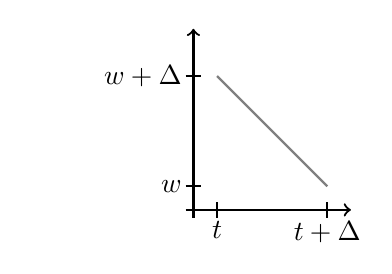
\begin{tikzpicture}[scale = 1]
\draw[->, thick] (-0.1,0) -- (2,0);
\draw[->,thick] (0,-0.1) -- (0,2.3);
\draw[-, thick] (0.3,-0.1) -- (0.3,0.1) node[inner sep=1pt,at start, anchor=north] (A)  {$t$};
\draw[-, thick] (1.7,-0.1) -- (1.7,0.1) node[inner sep=1pt,at start, anchor=north] (A)  {$t+\Delta$};
\draw[-, thick] (-.1,0.3) -- (0.1,0.3) node[inner sep=1pt,at start, left] (A)  {$w$};
\draw[-, thick] (-.1,1.7) -- (.1,1.7) node[inner sep=1pt,at start, left] (A)  {$\qquad\ \  w+\Delta$};
\draw[-, thick, color=gray!100] (0.3,1.7) -- (1.7,0.3);
\end{tikzpicture}
\caption{$Q_1:$ no arrivals.}
\end{subfigure}
\centering
\begin{subfigure}{.4\textwidth}
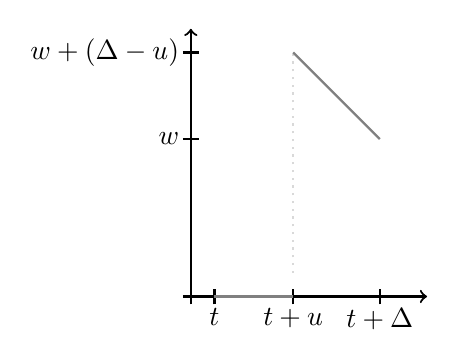
\begin{tikzpicture} [scale = 1]
\draw[->, thick] (-0.1,0) -- (3,0);
\draw[->,thick] (0,-0.1) -- (0,3.4);
\draw[-, thick] (0.3,-0.1) -- (0.3,0.1) node[inner sep=1pt,at start, anchor=north] (A)  {$t$};
\draw[-, thick] (1.3,-0.1) -- (1.3,0.1) node[inner sep=1pt,at start, anchor=north] (A)  {$t+u$};
\draw[-, thick] (2.4,-0.1) -- (2.4,0.1) node[inner sep=1pt,at start, anchor=north] (A)  {$t+\Delta$};

\draw[-, thick] (-.1,2) -- (0.1,2) node[inner sep=1pt,at start, left] (A)  {$w$};
\draw[-, thick] (-.1,3.1) -- (.1,3.1) node[inner sep=1pt,at start, left] (A)  {$w+(\Delta-u)$};
\draw[-, very thick, color=gray!100] (0.3,0) -- (1.3,0);
\draw[dotted, thick, color=gray!30] (1.3,0.3) -- (1.3,3.1);
\draw[-, thick, color=gray!100] (1.3,3.1) -- (2.4,2);
\end{tikzpicture}
\caption{$Q_2:$ arrival to empty queue.}
\end{subfigure}
\centering
\begin{subfigure}{.25\textwidth}
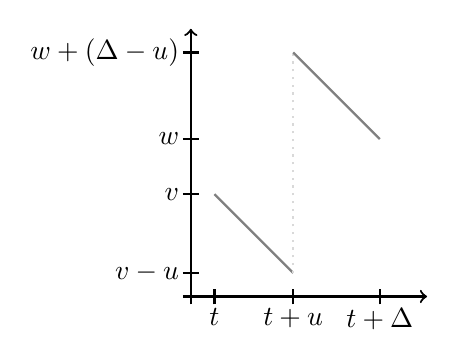
\begin{tikzpicture} [scale = 1]
\draw[->, thick] (-0.1,0) -- (3,0);
\draw[->,thick] (0,-0.1) -- (0,3.4);
\draw[-, thick] (0.3,-0.1) -- (0.3,0.1) node[inner sep=1pt,at start, anchor=north] (A)  {$t$};
\draw[-, thick] (1.3,-0.1) -- (1.3,0.1) node[inner sep=1pt,at start, anchor=north] (A)  {$t+u$};
\draw[-, thick] (2.4,-0.1) -- (2.4,0.1) node[inner sep=1pt,at start, anchor=north] (A)  {$t+\Delta$};

\draw[-, thick] (-.1,0.3) -- (0.1,0.3) node[inner sep=1pt,at start, left] (A)  {$v-u$};
\draw[-, thick] (-.1,1.3) -- (0.1,1.3) node[inner sep=1pt,at start, left] (A)  {$v$};
\draw[-, thick] (-.1,2) -- (0.1,2) node[inner sep=1pt,at start, left] (A)  {$w$};
\draw[-, thick] (-.1,3.1) -- (.1,3.1) node[inner sep=1pt,at start, left] (A)  {$w+(\Delta-u)$};
\draw[-, thick, color=gray!100] (0.3,1.3) -- (1.3,0.3);
\draw[dotted, thick, color=gray!30] (1.3,0.3) -- (1.3,3.1);
\draw[-, thick, color=gray!100] (1.3,3.1) -- (2.4,2);
\end{tikzpicture}
\captionsetup{width=.8\linewidth}
\caption{$Q_3:$ arrival to non-empty queue.}
\end{subfigure}
\caption{Graphical representation to illustrate \eqref{eq:Qi}, all ways one can have workload $w$ at time $t+\Delta$ (which are not $o(\Delta)$).} \label{fig:Q1Q2Q31}
\end{figure*}
We first let $t ,w > 0$ and $0 < \Delta < w$ be arbitrary. We now describe the possible evolution of the workload of the queue at the cavity in the interval $[t,t+\Delta]$ s.t.~it has exactly workload $w$ at time $t+\Delta$. We write:
\begin{equation}\label{eq:Qi}
f(t+\Delta, w) = Q_1 + Q_2 + Q_3 + o(\Delta),
\end{equation}
and describe how to obtain these $Q_i$.
\begin{itemize}
\item[($Q_1$)]  First, we consider the case where the queue at the cavity has $w+\Delta$ work at time $t$ and no potential arrivals in $[t,t+\Delta]$ make its workload increase. For this case we find:
$$
Q_1 = f(t,w+\Delta) - \lambda d \int_0^\Delta \int_{w+\Delta-u}^\infty c_d(t+u,w+\Delta-u,r) dr du.
$$
\item[($Q_2$)] Second, we consider the case in which the queue at the cavity is empty at time $t+u, u \in [0,\Delta]$ and its workload is increased to $w+(\Delta-u)$ by a potential arrival. This happens with density:
$$
Q_2 = \lambda d \int_0^\Delta C_d(t+u,w+(\Delta-u))\, du.
$$
\item[($Q_3$)] Lastly, the queue at the cavity may be non-empty at time $t+u, u \in [0,\Delta]$ and its workload increases to $w+(\Delta-u)$ by a potential arrival. This case has density:
$$
Q_3 = \lambda d \int_0^\Delta \int_u^{w+\Delta} c_d(t+u, v-u, w+(\Delta-u)) dv du.
$$
\end{itemize}
We graphically show the three options, $Q_1, Q_2$ and $Q_3$ in Figure \ref{fig:Q1Q2Q31}. Note that any other event involves having at least $2$ arrivals which yields terms that are $o(\Delta)$. Subtracting $f(t,w+\Delta)$, dividing by $\Delta$ and taking the limit $\Delta \rightarrow 0$ on both sides of \eqref{eq:Qi}, we find that \eqref{eq:PIDE1} indeed holds. 

We have not yet considered the case $w = 0$, for this we need to consider which events on $[t,t+\Delta]$ result in the workload of the queue at the cavity to be $0$ at time $t+\Delta$. To this end we consider the following scenarios:
\begin{itemize}
\item The queue at the cavity is empty at time $t$ and no actual arrivals occur in the interval $[t,t+\Delta]$. As each potential arrival is an actual arrival for empty queues, we find that this event occurs with probability $F(t,0) (1-\lambda d \Delta)$.
\item The queue at the cavity is non empty at some time $t+u, u \in [0,\Delta]$, and decreases to zero by time $t+\Delta$. We find that this event occurs with probability $\int_0^\Delta \int_0^{\Delta-v} f(t+u, v)\, dv \, du$.
\end{itemize}
\begin{figure*}
\hspace*{-2cm}
\begin{subfigure}{.25\textwidth}
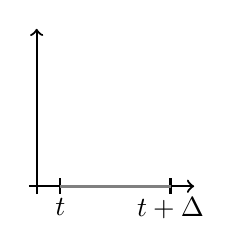
\begin{tikzpicture}[scale = 1]
\draw[->, thick] (-0.1,0) -- (2,0);
\draw[->,thick] (0,-0.1) -- (0,2.0);
\draw[-, thick] (0.3,-0.1) -- (0.3,0.1) node[inner sep=1pt,at start, anchor=north] (A)  {$t$};
\draw[-, thick] (1.7,-0.1) -- (1.7,0.1) node[inner sep=1pt,at start, anchor=north] (A)  {$t+\Delta$};
\draw[-, very thick, color=gray!100] (0.3,0) -- (1.7,0);
\end{tikzpicture}
\caption{Start off with an idle server.}
\end{subfigure}
\centering
\begin{subfigure}{.35\textwidth}
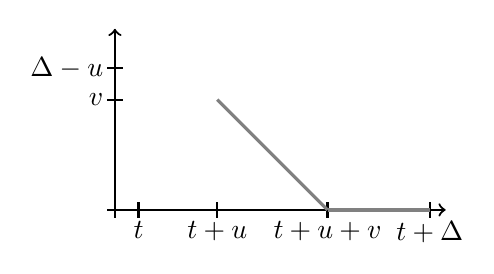
\begin{tikzpicture}[scale = 1]
\draw[->, thick] (-0.1,0) -- (4.2,0);
\draw[->,thick] (0,-0.1) -- (0,2.3);
\draw[-, thick] (0.3,-0.1) -- (0.3,0.1) node[inner sep=1pt,at start, anchor=north] (A)  {$t$};
\draw[-, thick] (1.3,-0.1) -- (1.3,0.1) node[inner sep=1pt,at start, anchor=north] (A)  {$t+u$};
\draw[-, thick] (2.7,-0.1) -- (2.7,0.1) node[inner sep=1pt,at start, anchor=north] (A)  {$t+u+v$};
\draw[-, thick] (4,-0.1) -- (4,0.1) node[inner sep=1pt,at start, anchor=north] (A)  {$t+\Delta$};
\draw[-, thick] (-.1,1.4) -- (.1,1.4) node[inner sep=1pt,at start, left] (A)  {$v$};
\draw[-, thick] (-.1,1.8) -- (.1,1.8) node[inner sep=1pt,at start, left] (A)  {$\Delta-u$};
\draw[-, very thick, color=gray!100] (1.3,1.4) -- (2.7,0);
\draw[-, very thick, color=gray!100] (2.7,0) -- (4,0);
\end{tikzpicture}
\caption{Start off with a non-idle server.}
\end{subfigure}
\centering
\caption{Graphical representation to illustrate all ways one can end up with an empty queue at time $t+\Delta$ (which are not $o(\Delta)$).} \label{fig:Q1Q2Q3}
\end{figure*}
Putting these together, we find that the following equality holds for $F(t+\Delta, 0)$:
$$F(t+\Delta, 0) = F(t,0)(1 - \lambda d \Delta) + \int_0^\Delta 
\int_0^{\Delta-u} f(t+v, u)\, dv\, du + o(\Delta).$$
Subtracting $F(t,0)$, dividing by $\Delta$ and taking the limit $\Delta \rightarrow 0$ on both sides results in \eqref{eq:PIDE2}.
\end{proof}
\end{theorem}
\begin{remark}
The PDIDE found in Theorem \ref{Thm:PIDE} could alternatively have been derived using the generalized Master Equation given by (7.25-7.26) in \cite{schuss2009theory}.
\end{remark}
We still require an exact expression for $c_d$ and $C_d$. Moreover, we need an efficient method to compute the quantities $\int_w^\infty c_d(t,w,r)\, dr$ and $\int_0^w c_d(t,u,w)\, du$. Therefore, in the next Proposition, we describe how to determine $c_d$ and $C_d$.
\begin{proposition}\label{prop:c_d}
For the \Redid\ policy we have $c_d(t,w,r)=c_{d,1}(t,w,r) + c_{d,2}(t,w,r) + c_{d,3}(t,w,r)$ such that:
\begin{align}
\int_w^\infty c_{d,1}(t,w,r)dr &= \bar{G}(w) f(t,w)(1-\bar{F}(t,0)^{d-1})\label{cd1}\\
\int_w^\infty c_{d,2}(t,w,r)dr &= f(t,w) \bar{F}(t,w)^{d-1}\label{cd2}\\
\int_w^\infty c_{d,3}(t,w,r)dr &= (d-1) f(t,w) \left(\bar{F}(t,\cdot)^{d-2} f(t,\cdot) * \bar{G}(\cdot)\right)(w)\label{cd3}\\
\int_0^w c_{d,1}(t,u,w) du &= g(w) \cdot (F(t,w) - F(t,0)) (1 - \bar{F}(t,0)^{d-1})\nonumber\\
\int_0^w c_{d,2}(t,u,w) du &= \left(g(\cdot) * f(t,\cdot)\bar{F}(t,\cdot)^{d-1}\right)(w)\nonumber\\
\int_0^w c_{d,3}(t,u,w) du &=
(d-1) F(t,w) \cdot \left(g(\cdot) * f(t,\cdot) \cdot \bar{F}(t,\cdot)^{d-2}\right)(w)\nonumber\\
&- (d-1) \left(g(\cdot) * F(t,\cdot) f(t,\cdot) \bar{F}(t,\cdot)^{d-2}\right)(w),\nonumber
\end{align}
where $(f_1*f_2)(w) = \int_0^w f_1(u) f_2(w-u) du$ denotes the convolution product. These quantities can all be computed quickly which simplifies solving (\ref{eq:PIDE1}-\ref{eq:PIDE2}) significantly. Lastly, we have $C_d(t,w)=F(t,0) \cdot g(w)$.
\begin{proof}
First we define $c_{d,1},c_{d,2}$ and $c_{d,3}$ as follows:
\begin{itemize}
\item At least one of the $d-1$ independent random variables with law $\mathcal{H}(t)$ is zero and the incoming job has size $r$. We find (for $w < r$):
\begin{align*}
c_{d,1}(t,w,r)\, dr\, ds &= g(r) f(t,w)(1-\bar{F}(t,0)^{d-1})\, dr\, ds.
\end{align*}
\item The queue at the cavity is the queue with the minimal workload (i.e.~$w$) and the size of the arrival is exactly $r-w$:
$$
c_{d,2}(t,w,r)\, dr\, dw = g(r-w) f(t,w) \bar{F}(t,w)^{d-1} \, dr\, dw.
$$
\item The queue with minimal workload has $0 < u < w$ workload, where $w$ is the workload of the queue
at the cavity, and the arrival size is $r-u$:
$$
c_{d,3}(t,w,r)\, dr\, ds = (d-1)f(t,w) \int_0^w g(r-u) \bar{F}(t,u)^{d-2}f(t,u) \,du\,dr\,dw.
$$
\end{itemize}
now the claimed equalities all follow from direct computation and applying Fubini (which is allowed as all integrands are positive functions). It is trivial to derive the expression for $C_d$.
\end{proof}
\end{proposition}
The PDIDE (\ref{eq:PIDE1}-\ref{eq:PIDE2}) can now be solved using an (improved) Euler scheme.  This result is also of interest to obtain 
a FPE for the equilibrium environment, i.e., workload distribution. 
In the subsequent section, we provide an efficient method to compute the equilibrium workload (and thus also response time) distribution.


\section{Equilibrium regime}\label{sec:equil_Redd}
For the equilibrium we use the same notations as in the transient case, but we leave out the time dependence, i.e., we write $f(w)$ instead of $f(t,w)$ and set $\frac{\partial f(w)}{\partial t} = 0$. From the PDIDE describing the transient behaviour (\ref{eq:PIDE1}-\ref{eq:PIDE2}) we now derive a method to compute the equilibrium workload distribution.
\begin{proposition}\label{thm:gen1}
The equilibrium workload distribution associated to the equilibrium environment of \Redid\ or \Redind\ satisfies the following equation:
\begin{align}
\bar{F}'(w)
=-f(w)
= - \lambda d \left( F(0) \bar{G}(w) + \int_0^w \int_w^\infty c_d(u,v) dv du \right) \label{fixpointF}
\end{align}
\begin{proof}
Integrating \eqref{eq:PIDE1} w.r.t.~$w$ and using \eqref{eq:PIDE2} as a boundary condition ($f(0^+)=\lambda d F(0)$), we obtain:
\begin{align}
f(w)
&= \lambda d \bigg( F(0) - \int_0^w C_d(u) du + \int_0^w \int_u^\infty c_d(u,r)\, dr\, du - \int_0^w \int_0^r c_d(u,r) \, du\, dr \bigg) . \label{eq:proofthmgen1.1}
\end{align}
We can further simplify \eqref{eq:proofthmgen1.1} by applying Fubini to the term $\int_0^w \int_0^r c_d(u,r)\, du\, dr$ to obtain \eqref{fixpointF}.
\end{proof}
\end{proposition}

\subsection{\Redid}
From Proposition \ref{thm:gen1} we obtain a simple DIDE which can be solved numerically:
\begin{theorem}\label{thm:mainRed}
The stationary workload distribution associated to the equilibrium environment satisfies the following DIDE:
\begin{align}
\bar{F}'(w)
&= -\lambda d \bigg[ \bar G(w) (1-\bar F(w)) + \int_0^w g(u) \bar F(w-u)^{d-1} (\bar F(w-u) - \bar F(w) )\, du\bigg]
.\label{eq:reddIDE}
\end{align}
\begin{proof}
Using (\ref{cd1}-\ref{cd3}) we can simplify \eqref{fixpointF} applied to \Redid\ to obtain:
\begin{align}
\bar F'(w)
&=-\lambda d \bigg[
\bar G(w) \left( (1-\bar F(0)^d) - \bar F(w) (1-\bar F(0)^{d-1}) \right)\nonumber\\
&+d (\bar G * f \bar F^{d-1})(w)-(d-1)\bar F(w) (\bar G * f \bar F ^{d-2})(w)
\bigg]\label{eq:proof_mainredid1}
\end{align}
We decompose the ccdf $\bar G = \bar G_1 + \bar G_2$, where $\bar G_1$ corresponds to the continuous part and $\bar G_2$ the discrete part. For the continuous part we apply integration by parts to obtain:
\begin{align}
(\bar G_1 * f \bar F^n)(w) &= \frac{1}{n+1} \bigg( \bar G_1(w)  \bar F^{n+1}(0) - \bar{G}_1(0) \bar F^{n+1}(w) + (g_1 * \bar F ^{n+1}) (w)\bigg). \label{eq:redIDE:cont}
\end{align}
For the discrete part we first define $\iota(w)=\sup\{n \mid a_n \leq w\}$, where $a_n$ for $n\in \{1,2,\dots\}$ are the atoms of the job size distribution. We find that the following equality holds:
\begin{align}
(\bar G_2 * f \bar F^n)(w) &=  \frac{1}{n+1} \bigg( \bar G_2(w) \bar F^{n+1}(0)  - \bar G_2(0) \bar F^{n+1}(w) + \sum_{n=0}^{\iota(w)} p_n \bar F^{n+1}(w-a_n)\bigg). \label{eq:redIDE:discr}
\end{align}
This equation follows by splitting the integral over the intervals $[0,a_0]$, $[a_0,a_1]$, $\dots$, $[a_{\iota(w)-1},a_{\iota(w)}]$, $[a_{\iota(w)},w]$. Putting integrands together and using the definition of $g$, we find that (\ref{eq:redIDE:cont}-\ref{eq:redIDE:discr}) simplifies to \eqref{eq:reddIDE}.
\end{proof}
\end{theorem}
The ccdf of the waiting time is given by $\bar F_W(w)=\bar F(w)^d$. The ccdf of the response time is given by the convolution of $g$ with the ccdf of the waiting time, i.e.~$\bar F_R(w) = \bar G(w) + (g * \bar F_W)(w)$.

The DIDE found in \eqref{eq:reddIDE} can be simplified to a set of ODEs in case job sizes have a PH distribution.
\begin{corollary}\label{cor:id_PH}
If job sizes have a PH distribution with parameters $(\alpha, A)$ then \eqref{eq:reddIDE} simplifies to the following ODE:
\begin{align*}
\bar{F}'(w) &= -\lambda d \alpha \left[ e^{wA}\textbf{1} (1-\bar F(w)) + \xi_1(w) - \xi_2(w) \bar F(w) \right]\\
\xi_1'(w) &= A\xi_1(w) + \mu \bar F^d(w)\\
\xi_2'(w) &= A\xi_2(w) + \mu \bar F^{d-1}(w),
\end{align*}
with $\mu = -A\textbf{1}$ and boundary condition $\xi_1(0)=\xi_2(0)=0$.
\begin{proof}
For PH distributed job sizes we find $\bar G(w)= \alpha e^{wA} \textbf{1}$ and $g(w) = \alpha e^{wA} \mu$. Applying this to \eqref{eq:reddIDE} and splitting terms, we find:
\begin{align}
\bar F'(w) &= -\lambda d \alpha \bigg[ e^{wA}\textbf{1} (1-\bar F(w)) + \int_0^w e^{uA} \mu \bar F (w-u) ^d \, du \nonumber\\
& - \int_0^w e^{uA} \mu \bar F(w-u)^{d-1}\, du \bar F(w)
\bigg]. \label{eq:PH_proof1}
\end{align}
Letting $\xi_1(w)=\int_0^w e^{uA} \mu \bar F^d(w-u)\, du=\int_0^w e^{(w-u)A} \mu \bar F^d(u)\, du$ we find:
\begin{align*}
\xi_1'(w)&=A\xi_1(w)+\mu \bar F^d(w).
\end{align*}
Analogously for $\xi_2(w)=\int_0^w e^{uA} \mu \bar F^{d-1}(w-u)\, du$ we find $\xi_2'(w)=A\xi_2(w)+\mu \bar F^{d-1}(w)$.
\end{proof}
\end{corollary}
\begin{remark}
We can generalize the result in Corollary \ref{cor:id_PH} to conditioned PH distributions. I.e.~let $X$ have PH distribution with parameters $(\alpha, A)$ and $a<b$ two positive numbers. If job sizes have distribution $(X \mid a<X<b)$ we find:
$$
\bar G(w) = \begin{cases}
1 & w<a\\
p\alpha (e^{Aw}-e^{Ab}) \textbf{1} & a \leq w < b\\
0 & b \leq w
\end{cases},
g(w) = \begin{cases}
0 & w<a\\
p\alpha e^{Aw} \mu & a \leq w < b\\
0 & b \leq w
\end{cases}
$$
with $p=\frac{1}{\alpha (e^{Aa}-e^{Ab}) \textbf{1}}$. This allows us to find the following DDE for the equilibrium workload distribution:
\begin{align*}
\bar F'(w) &= -\lambda d (1-\bar F(w)) & w \leq a\\
\bar F'(w) &= -\lambda d \left[
p\alpha (e^{Aw}-e^{Ab})\textbf{1}(1-\bar F(w)) + p \alpha (\xi_1(w) - \xi_2(w) \bar F(w))
\right] & a < w \leq b\\
\bar F'(w) &= -\lambda d p \alpha (\xi_1(w) - \xi_2(w) \bar F(w))& b<w,
\end{align*}
where $\xi_1, \xi_2$ satisfy $\xi_1(a)=\xi_2(a)=0$ and
\begin{align*}
\xi_1'(w) &= A\xi_1(w) + e^{Aa} \mu \bar F(w-a)^d & a < w \leq b\\
\xi_1'(w) &= A\xi_1(w) + (e^{Ab} \bar F(w-b)^d - e^{Aa} \bar F(w-a)^d) \mu & b < w\\
\xi_2'(w) &= A\xi_2(w) + e^{Aa} \mu \bar F(w-a)^{d-1} & a < w \leq b\\
\xi_2'(w) &= A\xi_2(w) + (e^{Ab} \bar F(w-b)^{d-1} - e^{Aa} \bar F(w-a)^{d-1}) \mu & b < w.\\
\end{align*} 
\end{remark}
\begin{remark}
It is not hard to see that when the job size distribution is some combination (product, sum, mixture, $\dots$) of discrete and PH-distributed random variables, one can still obtain a DDE by
generalizing Corollary \ref{cor:id_PH}.
\end{remark}
\color{black}
\subsection{\Redid\ with delayed cancellation} \label{sec:delay}
We now assume there is some delay in the cancellation of jobs, i.e.~after the first server finishes a job, the other $d-1$ servers continue working on the job for some time $\delta > 0$. We find the following result:
\begin{proposition} \label{prop:delay}
The stationary workload distribution associated to the equilibrium environment for \Redid\ with a cancellation delay equal to $\delta > 0$ satisfies the following DIDE:
\begin{align}
\bar F'(w) &= -\lambda d \left( \bar G(w) + \int_0^w g(w-u) \bar F(u)\, du - \bar F(w) \right) & w \leq \delta \label{eq:delay1}\\
\bar F'(w) &= -\lambda d \bigg( \bar G(w) - \bar F(w) \bar G(w-\delta) + \int_0^{\delta} \bar F(u) g(w-u) \, du\nonumber& \nonumber \\
& + \int_0^{w-\delta} \bar F(w-u-\delta)^{d-1} (\bar F(w-u) -\bar F(u)) g(u) \, du \bigg) & w > \delta. \label{eq:delay2}
\end{align}
\end{proposition}
\begin{proof}
It is not hard to see (analogue to Proposition \ref{prop:c_d}) that in this case we have:
\begin{align*}
c_d(w,r) \, dr \, ds &= g(r-\delta) f(w) (1-\bar F(0)^{d-1}) \, dr \, dw\\
&+ g(r-w) f(w) \bar F(w)^{d-1} \, dr \, ds\\
&+(d-1) f(w) \int_0^w g(r-u-\delta) \bar F(u)^{d-2} f(u) \, du \, dr \, dw.
\end{align*}
The result then follows using  arguments similar to the proof of Theorem \ref{thm:mainRed}.
\end{proof}
\begin{remark}
As for the Red$_{eq}$($d$) model, the ccdf of the waiting time is given by $\bar F_W(w) = \bar F(w)^d$ and the response time by $\bar F_R(w) = \bar G(w) + (g * \bar F_W)(w)$.
\end{remark}
The above DIDE simplifies to a DDE in case $X$ has a PH distribution:
\begin{corollary}
If job sizes have a PH distribution with parameters ($\alpha, A$), then the DIDE given by (\ref{eq:delay1}-\ref{eq:delay2}) simplifies to the following DDE:
\begin{align*}
\bar F'(w) &= -\lambda d (\bar G(w) + \alpha \xi_1(w) - \bar F(w)) & w \leq \delta\\
\bar F'(w) &= -\lambda d \bigg( \bar G(w) - \bar F(w) \bar G(w-\delta) + \alpha (\xi_1(w) + \xi_2(w) - \xi_3(w) \bar F(w)) \bigg) & w > \delta\\
\xi_1'(w) &= A \xi_1(w) + \bar F(w) \mu & w \leq \delta\\
\xi_1'(w) &= A \xi_1(w) & w > \delta\\
\xi_2'(w) &= \bar F(w-\delta)^{d-1} \bar F(w) \mu + A \xi_2(w) & w > \delta\\
\xi_3'(w) &= \bar F(w-\delta)^{d-1} \mu + A \xi_3(w) & w > \delta,
\end{align*}
with boundary condition $\xi_1(0) = \xi_2(\delta) = \xi_3(\delta) = 0$.
\end{corollary}
\begin{proof}
This follows from Proposition \ref{prop:delay} by defining :
\begin{align*}
\xi_1(w) & = \int_0^{\min\{w,\delta\}} e^{(w-u)A} \bar F(u) \, du \mu \\
\xi_2(w) &= \int_0^{w-\delta} F(u)^{d-1} \bar F(u+\delta) e^{(w-u-\delta)A} \, du \mu\\
\xi_3(w) &= \int_0^{w-\delta} \bar F(u)^{d-1} e^{(w-u-\delta)A} \, du \mu.
\end{align*}
\end{proof}
\color{black}

\subsection{\Redind}
If we were to analyse \Redind\ in the same manner as we did for \Redid , we would again find that the ccdf of the workload distribution satisfies equation \eqref{fixpointF}. In the case of \Redind , we find for arbitrary $0<w<r$:
\begin{equation}\label{eq:redind2}
c_d(w,r)=f(w) \cdot \left[ g(r-w) \bar F_{U+X}(r)^{d-1} + (d-1) \bar G(r-w) f_{U+X}(r) \bar F_{U+X}(r)^{d-2} \right],
\end{equation}
where $U$ and $X$ are random variables with distribution $F$ and $G$. Plugging \eqref{eq:redind2} in \eqref{fixpointF} one finds an FDE describing the workload distribution. This equation is hard to solve and it is not immediately clear how to simplify it. However, as shown in \cite{gardnerOR} the following result holds (the proof of which we summarize in a few words, for more details see \cite{gardnerOR}):
\begin{proposition}\label{prop:gardner}
The equilibrium workload distribution associated to \Redind\ satisfies the following DIDE:
\begin{align}
\bar F'(w)
&=
-\lambda d \bar{F}_{R_1}(w)^{d-1} (\bar F_{R_1}(w) - \bar F (w)), \label{eq:ind_copies}
\end{align}
with $\bar{F}_{R_1}(w) = \bar{G}(w) + (g * \bar F)(w)$, the probability that the response time is at least $w$ if a job is sent to only 1 server.
\begin{proof}
If one were to send only one replica,  this replica has a response time which is at least $w$ if and only if either the job size is at least $w$ or the job size is exactly $u<w$ and the workload of the queue to which the replica is sent is at least $w-u$. This shows that $\bar F_{R_1}(w) = \bar G(w) + (g * \bar F)(w)$.

The probability that a potential arrival increases the workload of the queue at the cavity from a value under $w$ to a value above $w$ is equal to the probability that all $d-1$ replicas which are sent to other queues have a response time which is at least $w$, the response time of the replica sent to the queue at the cavity is at least $w$ and the queue at the cavity has a workload which is at most $w$. Note that the individual response times $R_1$ can be written as a product because of the independence assumption of both the workload processes and the job sizes.
\end{proof}
\end{proposition}
For PH-distributed job sizes we find a result which is similar to Corollary \ref{cor:id_PH}:
\begin{corollary}\label{cor:ind_PH}
If job sizes have a PH distribution with parameters $(\alpha, A)$ then \eqref{eq:ind_copies} simplifies to the following ODE:
\begin{align*}
\bar F'(w)
&=
-\lambda d (\bar G(w) + \alpha \xi(w))^{d-1} \left( \bar G(w) + \alpha \xi(w) - \bar F(w) \right),\\
\xi'(w)
&=
A\xi(w) + \bar F(w) \mu,
\end{align*}
with $\mu = -A\textbf{1}$ and boundary condition $\xi(0)=0$.
\end{corollary}
\begin{proof}
This follows in a similar manner as Corollary \ref{cor:id_PH}, but here we set $\xi(w)= \int_0^w e^{(w-u) A} \mu \bar F(u)\, du$.
\end{proof}
\begin{remark}
One can again generalize this result to conditional PH-distributions and combinations of PH-distributions and discrete distributions.
\end{remark}
In case of independent replicas there are several possible definitions for the waiting time, that is,
it could be the time until the first replica enters service or the time until the replica that
first completes service enters service. As such we only consider the response time, the ccdf of which 
is:
$$
\bar F_R(w)=\left(\bar G(w)+(g*\bar F)(w)\right)^d \left(=\bar{F}_{R_1}(w)^d\right).
$$

\subsection{Numerical considerations}\label{sec:algorithm}
Throughout all sections which contain numerical examples, we exclusively make use of job size distributions which have a mean equal to one. In particular we focus our attention to the following job size distributions:
\begin{itemize}
\item \textit{Exponential Job Sizes : } Job sizes have an exponential distribution with mean equal to one.
\item \textit{Deterministic Job Sizes : } Job sizes are always equal to one.
\item \textit{Bounded Pareto Job Sizes : } Job sizes are bounded Pareto with lower bound $0.2$, upper bound $72$ and $\alpha=1.1$, meaning $\E[G]=1$ and $\E[G^2]=10$.
\item \textit{Hyperexponential Job Sizes : } Job sizes are hyperexponential with two phases and balanced means, chosen such that $\E[G]=1$. When the SCV is not specified, we set $\E[G^2]=10$.
\item \textit{Erlang Job Sizes : } Job sizes which have an Erlang-$k$ distribution with $2$ up to $50$ phases such that $\E[G]=1$.
\end{itemize}
\begin{remark}
For bounded Pareto job sizes, we need to resort to solving a DIDE which is $O(M^2)$, for all other job size distributions the required computation time is only $O(M)$. Here $M$ denotes the number of control points used to numerically represent $\bar F$.
\end{remark}
\subsection*{Obtaining the system load $\bar F(0)$}
Note that Theorem \ref{thm:mainRed}, Corollary \ref{cor:id_PH}, Proposition \ref{prop:gardner} and Corollary \ref{cor:ind_PH} do not specify a boundary condition for $\bar F(0)$. This is not surprising as $\bar F(0)$ corresponds to the unknown actual system load. We have the following Lemma which is used as a basis for an algorithm to find $\bar F(0)$:
\begin{lemma}\label{lem:numerical}
Let $\lambda > 0, d \in \{2,3,\dots\}$ be such that the associated system is stable then the following are equivalent:
\begin{itemize}
\item $\bar F(w)$ is a solution to \eqref{eq:reddIDE} resp.~\eqref{eq:ind_copies} and $\inf_{w>0} \bar F(w) = 0$,
\item $\bar F(w)$ is the unique ccdf of the workload equilibrium for \Redid\ resp.~\Redind.
\end{itemize}
\end{lemma}
\begin{proof}
Obviously, if $\bar F(w)$ is the ccdf of the workload equilibrium, it is a solution to the associated FPE and thus also of the associated DIDE, moreover $\inf_{w>0} \bar F(w)=0$ holds for any ccdf.

We should still show that the solution $\bar F$ is indeed a ccdf if it is a solution to \eqref{eq:reddIDE} or \eqref{eq:ind_copies} and $\inf_{w>0} \bar F(w) = 0$. The uniqueness then follows from Conjecture \ref{conj1}.  We show that for arbitrary $t>0$, we have: if for all $w<t, \bar F'(w) \leq 0$ and $\bar F (w) \geq 0$ then $\bar F'(t) \leq 0$, this shows that $\bar F$ is a decreasing function as it is positive. For \eqref{eq:reddIDE} it suffices to note that $\bar F(t-u) - \bar F(t)$ appearing in the integral equals $- \int_{t-u}^t \bar F'(v)\, dv \geq 0$. For \eqref{eq:ind_copies} we note that:
\begin{align*}
F_{R_1}(t)
&= \bar G(t) + \int_0^t \bar F(u) g(t-u) \, du\\
&\geq \bar G(t) + \int_0^t \bar F(t) g(t-u) \, du\\
&= \bar G(t) + G(t) \bar F(t)\\
&\geq \bar F(t).
\end{align*} 
We have thus shown that if $\bar F$ satisfies the stated conditions, it is also a non-increasing function, as $\inf_{w>0} \bar F(w)=0$ we find that $\lim_{w\rightarrow \infty} \bar F(w)=0$. This shows that $\bar F$ is indeed a ccdf.
\end{proof}
Based on the result shown in Lemma \ref{lem:numerical} we obtain an algorithm which can be used to find the ccdf $\bar{F}$ which is the solution  for \eqref{eq:reddIDE} and \eqref{eq:ind_copies}. Also, we present a simple method to check whether for a given job size distribution, $\lambda$ and $d$ the system is stable (i.e.~the equilibrium workload distribution is not infinite). Note that the DIDE however still makes sense when the system is unstable: we find the boundary condition $\bar F(0)=1$ and from this it is not hard to see that both for \Redid\ and \Redind\ we find $\bar F(w) =1$ for all $w$, i.e.~the system load is almost surely infinite.

We employ the following bisection algorithm to find the value of $\bar F(0)$ for which the associated solution satisfies $\inf_{w>0} \bar F(w)=0$:
\begin{enumerate}
\item Set $\textup{lb}=0$ and $\textup{ub}=1$,
\item Compute $y=\inf_{w>0} \bar F(w)$, where $\bar F(w)$ is computed as the solution of \eqref{eq:reddIDE} or \eqref{eq:ind_copies}, with boundary condition $\bar F(0) = x_0 = \frac{\textup{lb} + \textup{ub}}{2}$.
\item Set $\textup{lb}=x_0$ if $y<0$ otherwise set $\textup{ub}=x_0$, return to Step 2.
\end{enumerate}
Due to Lemma \ref{lem:numerical}, we are certain this algorithm converges, provided that $\inf_{w>0} \bar F(w)$ is increasing as a function of the boundary condition $\bar F(0)$. Actually all we need is if $\bar F_1(0) < \bar F_2(0)$ and $\inf_{w>0} \bar F_2(w) < 0$ then $\inf_{w>0} \bar F_1(w) < 0$. Unfortunately this
statement appears to be hard to prove and we only managed to confirm this  numerically 
(see also Figure \ref{fig:convergence_alg3} and Section \ref{sec:open_binary_redd}).

We now provide some deeper insight into how well the algorithm performs. For this discussion let us focus on \Redid\ and note that the discussion for \Redind\ is completely analogous. We need to numerically solve \eqref{eq:reddIDE} for each step of the algorithm, which takes $O(N^2)$ resp.~$O(N)$ time for continuous resp.~discrete or PH distributed job sizes (use Corollary \ref{cor:id_PH}). For a function $f$, we let $\|f\|_\infty=\sup_{w>0}|f(w)|$ denote its supremum norm. In Figure \ref{fig:convergence_alg1}, we first compute the limiting distribution $\bar F_{\infty}$ which satisfies \eqref{eq:reddIDE} and $\bar F(0)$ is chosen such that $|\inf_{w>0} \bar F(w)| < 10^{-10}$. We let $\bar F_n$ denote the solution to \eqref{eq:reddIDE} after $n$ steps have been taken in the algorithm. We show the difference $\|\bar F_n - \bar F_\infty\|_\infty$ for $n$ varying from $1$ to $34$ (note that $34$ is the first value $n$ for which $2^{-n}<10^{-10}$). Figure \ref{fig:convergence_alg1.1} is for exponential job sizes, $\lambda = 0.48$ and $d=2,3,4,5$ while Figure \ref{fig:convergence_alg1.2} is for $d=2$, $\lambda = 0.7$ and varying (i.e.~exponential, deterministic, bounded Pareto and hyperexponential) job sizes. We observe that the accuracy of $\bar F_n$ increases exponentially which means that $\|\bar F_n - \bar F_{\infty}\|_\infty \approx  |\bar F_n(0) - \bar F_\infty(0)|$.
\begin{figure*}[t]
\begin{subfigure}{.45\textwidth}
\centering
\includegraphics[width=0.9\textwidth]{figures/Chapter3/plot_convergence1.pdf}
\caption{Exponential Job Sizes with $\lambda=0.48$.}
\label{fig:convergence_alg1.1}
\end{subfigure}
\begin{subfigure}{.45\textwidth}
\centering
\includegraphics[width=0.9\textwidth]{figures/Chapter3/plot_convergence2.pdf}
\caption{Varying job sizes, $d=2$ and $\lambda =0.7$.}
\label{fig:convergence_alg1.2}
\end{subfigure}
\caption{Convergence of $\bar F_n$, the ccdf found after $n$ steps to the limiting distribution ccdf $\bar F_{\infty}$.}
\label{fig:convergence_alg1}
\end{figure*}
We now show $\bar F_n$ for $n=1,\dots,34$ in Figure \ref{fig:convergence_alg2} (on a logarithmic scale, negative values are discarded). Rather than labelling each line, we increase the linewidth as $n$ increases. We clearly observe that as $n$ increases, $\bar F_n$ gets increasingly closer to being an actual ccdf. Moreover we see that none of the lines cross, which supports the claim that if $\bar F_1(0) < \bar F_2(0)$, then for all $w: \bar F_1(w) < \bar F_2(w)$.

\begin{figure*}[t]
\begin{subfigure}{.45\textwidth}
\centering
\includegraphics[width=0.9\textwidth]{figures/Chapter3/plot_convergence3.pdf}
\caption{Bounded Pareto Job Sizes.}
\label{fig:convergence_alg2.1}
\end{subfigure}
\begin{subfigure}{.45\textwidth}
\centering
\includegraphics[width=0.9\textwidth]{figures/Chapter3/plot_convergence4.pdf}
\caption{Exponential Job Sizes.}
\label{fig:convergence_alg2.2}
\end{subfigure}
\caption{Plot of $\bar F_n$ with $n=1,\dots,34$, $\lambda = 0.7$ and $d=2$ for bounded Pareto resp.~exponential job size distributions. The linewidth is increased with $n$.}
\label{fig:convergence_alg2}
\end{figure*}
In Figure \ref{fig:convergence_alg3} we show $\inf_{w>0} \bar F(w)$, where $\bar F$ is the solution of \eqref{eq:reddIDE} as a function of the used initial value $\bar F(0)$. In Figure \ref{fig:convergence_alg3.1}, job sizes are deterministic, $\lambda = 0.4$ and $d=2,3,4,5$. Here we observe that for certain values of $\lambda, d$ and $\bar F(0)$ the infimum might be $-\infty$, but it is clearly monotone increasing and close to linear with a steeper ascend close to $\bar F(0)=1$. In fact,
all of these curves converge to $1$ as $\bar F(0)$ converges to $1$ and  
the incline close to $1$ is so steep that it is not even visible in Figure \ref{fig:convergence_alg3}. 
In Figure \ref{fig:convergence_alg3.2}, bounded Pareto job sizes are used with $d=2$ and $\lambda = 0.1,0.3,0.5,0.7$, we observe the same behaviour as for deterministic job sizes: the trajectory is close to linear with a steep incline when $\bar F(0)$ gets close to one. This curve, let us denote it by $y=f(x)$, is in fact the one for which we need to find the value $x_0$ that satisfies $f(x_0)=0$ (i.e.~this value $x_0$ is exactly the $\bar F(0)$ boundary condition for which $\bar F$ becomes a ccdf). The system is deemed unstable if and only if $y=f(x)$ does not cross zero in $[0,1]$ and this happens when $f(x) < 0$ for all $x \in [0,1)$, meaning there is a discontinuity in $1$ as we necessarily have
$f(1)=1$ as mentioned before. Moreover, as $y=f(x)$ is a curve which is close to linear, better (i.e.~faster) algorithms could be used to obtain a root of $f$, e.g.~a simple Newton iteration would converge extremely fast in this case.

\subsection*{Obtaining the stability region $\lambda_{\max}$}
Let $\lambda_{\max}$ be defined as the highest value value of $\lambda$ for which a system is still stable. That is, for any $\lambda < \lambda_{\max}$ the system is stable whilst for any $\lambda \geq \lambda_{\max}$ it is unstable. We know that for \Redid , $\lambda_{\max} \in [1/d, 1]$. To obtain an algorithm which allows to compute $\lambda_{\max}$ we note that if we pick $\varepsilon > 0$ small and we find $\lambda > 0$ such that for this $\lambda$ and $\bar F(0) = 1-\varepsilon$ we have $\inf_{w>0} \bar F(w) = 0$, then the system load for this $\lambda$ is $1-\varepsilon$. If we now pick $\varepsilon > 0$ small enough this means that the system is close to instability, and this value can then be used as an approximation for $\lambda_{\max}$. We verify this method in Section \ref{sec:verification_stability} where we show that the approximation of $\lambda_{\max}$ obtained in this manner is at least accurate up to $0.001$.

\begin{figure*}[t]
\begin{subfigure}{.45\textwidth}
\centering
\includegraphics[width=0.9\textwidth]{figures/Chapter3/plot_convergence5.pdf}
\caption{Deterministic Job Sizes and $\lambda=0.4$.}
\label{fig:convergence_alg3.1}
\end{subfigure}
\begin{subfigure}{.45\textwidth}
\centering
\includegraphics[width=0.9\textwidth]{figures/Chapter3/plot_convergence6.pdf}
\caption{Bounded Pareto Job Sizes and $d=2$.}
\label{fig:convergence_alg3.2}
\end{subfigure}
\caption{Plot of $\inf_{w>0} \bar F(w)$ as a function of $\bar F(0)$ for the solution of \eqref{eq:reddIDE}.}
\label{fig:convergence_alg3}
\end{figure*}
\section{Validation of the model}\label{sec:finAcc_Tompecs}
\subsection{Finite system accuracy}
In this section we use the algorithm presented in Section \ref{sec:algorithm} to find the limiting workload distribution for \Redid\ , where we find the value of $\bar F(0)$ such that $\bar F$ is a ccdf.

We compare the equilibrium workload distribution with the simulated workload distribution for a finite system with $N$ servers. We do this for $4$ of the main job size distributions: exponential, deterministic, bounded Pareto and hyperexponential. All simulation runs simulate the system up to time $t=10^7/N$ and use a warm-up period of $30\%$. We simulate a system of $N=10,50,250$ servers. The results are shown in Figure \ref{fig:accuracy}. We see that as $N$ increases the approximation provided by the DIDE becomes more accurate (which supports Conjecture \ref{conj1}). Note that a similar figure can easily be made for the response time distribution and \Redind .

\begin{figure*}[t]
\begin{subfigure}{.45\textwidth}
\begin{center}
\includegraphics[width=0.9\textwidth]{figures/Chapter3/Exp1d2N1050250WLlam07.pdf}
\caption{$\lambda=0.7,$ exponential job sizes.}
\label{fig:validateEXP}
\end{center}
\end{subfigure}
\begin{subfigure}{.45\textwidth}
\begin{center}
\includegraphics[width=0.9\textwidth]{figures/Chapter3/Det1d2N1050250WLlam06.pdf}
\caption{$\lambda=0.6,$ deterministic job sizes.}
\label{fig:validateDET}
\end{center}
\end{subfigure}
\vspace*{4mm}
\begin{subfigure}{.45\textwidth}
\begin{center}
\includegraphics[width=0.9\textwidth]{figures/Chapter3/BoundedParetolb02ub72alpha11lam07d2.pdf}
\caption{$\lambda=0.7$, bounded Pareto job sizes (max=72).}
\label{fig:validatePAR}
\end{center}
\end{subfigure}
\begin{subfigure}{.45\textwidth}
\begin{center}
\includegraphics[width=0.9\textwidth]{figures/Chapter3/HEXPSCV9f05lam07d2.pdf}
\caption{$\lambda=0.7,$ hyperexponential job sizes.}
\label{fig:validateHEXP}
\end{center}
\end{subfigure}
\caption{For the \Redid\ policy: Limiting workload distribution vs.~simulation 
	for $N$ servers.
	The full line represents the solution of the DIDE/DDE/ODE, which is compared with the simulated $95\%$ confidence intervals.}\label{fig:accuracy}
\end{figure*}
\subsection{Stability region}\label{sec:verification_stability}
\begin{figure*}[t]
\begin{subfigure}{.45\textwidth}
\begin{center}
\includegraphics[width=0.9\textwidth]{figures/Chapter3/plots_stable.pdf}
\caption{Arrival rate $\lambda = \lambda_{\max}-0.001$, where $\lambda_{\max}$ depends on the job size distribution.}
\label{fig:stab_ver1}
\end{center}
\end{subfigure}
\begin{subfigure}{.45\textwidth}
\begin{center}
\includegraphics[width=0.9\textwidth]{figures/Chapter3/plots_unstable.pdf}
\caption{Arrival rate $\lambda = \lambda_{\max}+0.001$, where $\lambda_{\max}$ depends on the job size distribution.}
\label{fig:stab_ver2}
\end{center}
\end{subfigure}
\caption{The mean workload of a simulated system with $N=300$ servers, $d=2$ and deterministic, exponential resp.~hyperexponential job sizes.}
\label{fig:stab_ver}
\end{figure*}

In this section we apply the algorithm presented in Section \ref{sec:algorithm} to obtain the maximum value $\lambda_{\max}$ for which the system is still stable. For this purpose, we first compute the value of $\lambda_{\max}$ for a system with $d=2$ and deterministic, exponential resp.~hyperexponential job sizes. We find:
\begin{itemize}
\item $\lambda_{\max} = 0.80554\dots$ for deterministic job sizes,
\item $\lambda_{\max} = 0.81669\dots$ for exponential job sizes,
\item $\lambda_{\max} = 0.83441\dots$ for hyperexponential job sizes.
\end{itemize}
Note that in this example $\lambda_{\max}$ increases as the job size variability increases.
For each distribution, we set $\lambda=\lambda_{\max}-0.001$ and simulate a system with $N=300$, arrival rate $\lambda$ and the corresponding job size distribution for a time of $2\cdot 10^4$. We observe in Figure \ref{fig:stab_ver1} that the system  indeed appears to be stable. In Figure \ref{fig:stab_ver2} we observe that, when taking arrival rate $\lambda=\lambda_{\max}+0.001$ and simulating the system with $N=300$ seems to result in an unstable system for each job size distribution. This suggests that our method to obtain $\lambda_{\max}$ is indeed quite accurate.

\section{Numerical experiments for \Redid}\label{sec:numerical}
\subsection{Mean response time and workload distribution}\label{sec:MRT_WL_ind}
\begin{figure*}[t]
\begin{subfigure}{.45\textwidth}
\begin{center}
\includegraphics[width=0.9\textwidth]{figures/Chapter3/plot_WL_ifo_lam_diffdists_id.pdf}
\caption{$d=2$ and different job size distributions.}
\label{fig:workloaddiffjobs}
\end{center}
\end{subfigure}
\begin{subfigure}{.45\textwidth}
\begin{center}
\includegraphics[width=0.9\textwidth]{figures/Chapter3/plotworkloadBPd2345.pdf}
\caption{$d=2,3,4,5$ and bounded Pareto job sizes.}
\label{fig:workloaddiffd}
\end{center}
\end{subfigure}
\caption{Workload $\bar{F}(0)$ as a function of the arrival rate $\lambda$ for \Redid .}
\label{fig:workload}
\end{figure*}

\begin{figure*}[t]
\begin{subfigure}{.45\textwidth}
\begin{center}
\includegraphics[width=0.9\textwidth]{figures/Chapter3/test.png}
\caption{$d=2$ and different job size distributions.}
\label{fig:MRTdiffjobsizes}
\end{center}
\end{subfigure}
\begin{subfigure}{.45\textwidth}
\begin{center}
\includegraphics[width=0.9\textwidth]{figures/Chapter3/test2.png}
\caption{$d=2,3,4,5$ and bounded Pareto job sizes.}
\label{fig:MRTdiffd_eq}
\end{center}
\end{subfigure}
\caption{Mean response time $\E[R] = \left(1+\int_0^\infty \bar{F}(w)^d ds\right)$ as a function of the arrival rate $\lambda$ for \Redid .}
\label{fig:MRT}
\end{figure*}

In Figures \ref{fig:workload} and \ref{fig:MRT} we show the actual workload $\bar{F}(0)$ and the mean response time $\E[R]=1+\int_0^\infty \bar{F}(w)^d \, ds$ of the \Redid\ policy as a function of the arrival rate $\lambda$ (recall $\E[G]=1$).
From Figure \ref{fig:workloaddiffjobs}, it is clear that the stability region not only depends on the mean and the variance of the job size distribution, but also on higher moments (as $\E[G^2]=10$ for both the bounded Pareto and hyperexponential job sizes, see also Figure \ref{fig:lam_max_red2}). This makes the question of stability for \Redid\ for general job size distributions a hard problem (which in turn makes proving Conjecture \ref{conj1} hard). We can already infer from the plot that the more variable the job size distribution, the lower the associated workload.
From Figure \ref{fig:workloaddiffd}, it is obvious that $\lambda_{\max}$ (defined as the supremum of the arrival rates $\lambda$ for which $\bar F(0) < 1$) decreases and the workload increases as a function of $d$ (we have numerically verified that this also holds for the other job size distributions considered). For a more detailed discussion on $\lambda_{\max}$, see Section \ref{sec:stab_id}. Note that, as one would expect from a system that employs redundancy, the workload increases as a concave function as the arrival rate $\lambda$ increases.

We show in Figure \ref{fig:MRTdiffjobsizes} that, despite the fact that the workload for the less variable jobs is consistently higher than that of the more variable ones, the same does not hold for the response times. We see that adding variability to the job size distribution also increases the mean response time (for $\lambda$ sufficiently bounded away from instability).
From Figure \ref{fig:MRTdiffd_eq} it is clear that only for small values of $\lambda$ there is a reduction in response time by increasing $d$: this reduction is due to the fact that for small arrival rates a job is more likely to find an idle server by increasing $d$, but as $\lambda$ increases higher values of $d$ cause too much extra load on the servers which causes an increased response time. In all plots in Figure \ref{fig:MRT} we observe that mean response times stay relatively small until $\lambda$ is close to $\lambda_{\max}$ at which point the mean response time explodes to infinity. This effect is more visible as the SCV of the jobs decreases and as the value of $d$ increases.
\subsection{Impact of the job size variability}\label{sec:ifo_SCV}
\begin{figure*}[t]
\begin{subfigure}{.45\textwidth}
\begin{center}
\includegraphics[width=0.9\textwidth]{figures/Chapter3/plot_MRT_Erlang_identical_diffd.pdf}
\caption{Erlang job sizes with mean one and SCV on the $x$-axis.}
\label{fig:MRT_Erlangs_identical}
\end{center}
\end{subfigure}
\begin{subfigure}{.45\textwidth}
\begin{center}
\includegraphics[width=0.9\textwidth]{figures/Chapter3/plot_ifo_SCV_Redid_HExp_vard.pdf}
\caption{Hyperexponential job sizes with balanced means, mean one and the SCV on the $x$-axis.}
\label{fig:MRTdiffd}
\end{center}
\end{subfigure}
\caption{Mean response time $\E[R] =\left(1+\int_0^\infty \bar{F}(w)^d ds\right)$ as a function of the job sizes' SCV for $d=2,3,4,5$ and $\lambda=0.45$.}
\label{fig:ifo_SCV_vard}
\end{figure*}
We now investigate how well \Redid\ behaves as a function of the job sizes distribution's SCV. In Figure \ref{fig:ifo_SCV_vard} we show the mean response time as a function of the job sizes' SCV. On $[0,1]$ we use deterministic, Erlang and exponential job sizes with mean one (see Figure \ref{fig:MRT_Erlangs_identical}), while on $(1,40]$ we use a hyperexponential distribution with balanced means and mean one (see Figure \ref{fig:MRTdiffd}). In both figures, we fix $\lambda=0.45$ and $d=2,3,4,5$. We observe that the mean response time generally increases more or less linearly 
as a function of the SCV.
The most notable exception occurs when $d=5$ and the SCV is close to zero. In this case 
$\E[R]$ decreases as the system with deterministic jobs is close to instability and increasing the job size variability somewhat increases the value of $\lambda_{\max}$, which causes $E[R]$ to decrease.  Moreover, we observe that increasing $d$ in case of deterministic job sizes also increases the mean response time, whilst for large SCV this is not necessarily the case. This makes sense as for jobs with low variability, the risk of picking a server that is serving a large job is smaller than for more variable jobs, meaning there is less incentive to increase $d$ and increasing $d$ also increases the amount of work on the servers. 

\begin{figure*}[t]
\begin{subfigure}{.45\textwidth}
\begin{center}
\includegraphics[width=0.9\textwidth]{figures/Chapter3/plot_MRT_Erlang_identical_difflam.pdf}
\caption{$d=2$, $\lambda=0.4,0.5,0.6,0.7,0.8$ and Erlang job sizes with mean one and SCV on the $x$-axis.}
\label{fig:MRT_ifo_SCV_difflam_Erlangs}
\end{center}
\end{subfigure}
\begin{subfigure}{.45\textwidth}
\begin{center}
\includegraphics[width=0.9\textwidth]{figures/Chapter3/plot_ifo_SCV_Redid_HExp.pdf}
\caption{$d=2$, $\lambda=0.4,0.5,0.6,0.7,0.8$ and hyperexponential job sizes with mean one and SCV on the $x$-axis.}
\label{fig:MRT_ifo_SCV_difflam_HExp}
\end{center}
\end{subfigure}
\caption{Mean response time $\E[R] =\left(1+\int_0^\infty \bar{F}(w)^d ds\right)$ as a function of the job sizes' SCV.}
\label{fig:MRT_ifo_SCV_difflam}
\end{figure*}
In Figure \ref{fig:MRT_ifo_SCV_difflam} we make the same plots as in Figure \ref{fig:ifo_SCV_vard}, but now instead of fixing $\lambda$ and taking multiple values of $d$, we fix $d=2$ and consider multiple values of $\lambda$. As expected, we observe that increasing $\lambda$ also increases the mean response time and the slope of $\E[R]$ as a function of the SCV. Moreover we again observe that a decrease for low job size variability occurs when the system is close to instability.

\subsection{Stability}\label{sec:stab_id}
\begin{figure*}[t]
\begin{subfigure}{.45\textwidth}
\begin{center}
\includegraphics[width=0.9\textwidth]{figures/Chapter3/plot_ifo_d1.pdf}
\caption{Deterministic job sizes.}
\label{fig:lam_max_red1}
\end{center}
\end{subfigure}
\begin{subfigure}{.45\textwidth}
\begin{center}
\includegraphics[width=0.9\textwidth]{figures/Chapter3/plot_ifo_d2.pdf}
\caption{The difference between exponential (exp), bounded Pareto (BP) and hyperexponential (HE) job sizes and deterministic (det) job sizes.}
\label{fig:lam_max_red2}
\end{center}
\end{subfigure}
\caption{The evolution of $\lambda_{\max}$ as a function of $d$ for deterministic, exponential, bounded Pareto and hyperexponential job sizes in the \Redid\ model.}
\label{fig:lam_max_red}
\end{figure*}
Let $\bar F$ satisfy \eqref{eq:reddIDE}, we then find for all $t$ for which $\bar F(w) \geq 0, w \in [0,t]$:
$$
\bar{F}'(w) \leq -\lambda d \bar G(w) (1-\bar F(w)).
$$
This shows that, if there exists an $\varepsilon>0$ for which $\bar G(\varepsilon)>0$ (i.e.~job sizes are not identically zero) and $\bar F(0) < 1$, then in the limit $d\rightarrow \infty$ we find that $\bar F(w)$ falls off at an unbounded speed. This shows that as $d$ tends to infinity, $\lambda_{\max}$ tends to zero. It is also intuitively clear that this is the case as for $d=N$ we find that \Redid\ becomes an M/G/1 queue with arrival rate $\lambda N$ where $N$ tends to infinity.

This fact is also reflected in Figure \ref{fig:lam_max_red1}, where we show the evolution of $\lambda_{\max}$ as a function of $d$ for \Redid\ with deterministic job sizes. We observe that for $d=1$, $\lambda_{\max}=1$ (naturally as this is simply an M/D/1 queue), as $d$ increases there is first a sharp drop in $\lambda_{\max}$ until $\lambda_{\max} \approx 0.2$ around $d=20$ after which we see that the curve slowly converges to its horizontal asymptote at $\lambda_{\max}=0$.

In Figure \ref{fig:lam_max_red2}, we compare the value of $\lambda_{\max}$ for other job sizes to $\lambda_{\max}$ for deterministic job sizes. We observe that the difference starts at zero (as for any M/G/1 queue $\lambda_{\max}=1$), then jumps up for $d=2$ and $d=3$ after which it decays to zero. We observe that the difference in stability region increases as the tail of the job size distribution is more fat. The difference in $\lambda_{\max}$ is however fairly modest (no larger than $0.06$).

\subsection{Variance of the response time distribution}
\begin{figure*}[t]
\begin{subfigure}{.45\textwidth}
\begin{center}
\includegraphics[width=0.9\textwidth]{figures/Chapter3/plotVarRTDet.pdf}
\caption{Deterministic job sizes.}
\label{fig:var_det}
\end{center}
\end{subfigure}
\begin{subfigure}{.45\textwidth}
\begin{center}
\includegraphics[width=0.9\textwidth]{figures/Chapter3/plotVarRTExp.pdf}
\caption{Exponential job sizes.}
\label{fig:var_discr}
\end{center}
\end{subfigure}
\caption{The variance of the Response time distribution as a function of the arrival rate $\lambda$ for $d=2,3,4,5$ in the \Redid\ model.}
\label{fig:var_id}
\end{figure*}
We now take a closer look at the behaviour of the variance of the response time distribution. To compute the variance, it is best to first compute the ccdf of the squared response time $\bar F_{R^2}$ and then integrate, i.e.~we compute the variance as:
$$\textup{Var}(R) = \int_0^\infty \bar F_{R^2}(w)\, dw - \left(\int_0^\infty \bar F_R(w)\, ds\right)^2.$$
This is numerically more stable as it avoids the need to differentiate $\bar F_R$ to obtain its density $f_R$. Do note that the computation of $\bar F_{R^2}$ requires a quadratically wider $w$ range $[0,w_{\max}]$ than $\bar F_R$ in order to ensure that $\bar F_{R^2}(w_{\max})$ is sufficiently small.

In Figure \ref{fig:var_id} we show the variance of the response time distribution as a function of the arrival rate $\lambda$ for deterministic and exponential job sizes. We observe in Figure \ref{fig:var_det} that $\textup{Var}(R)$ remains very small until it explodes when $\lambda$ approaches $\lambda_{\max}$. As long as $\lambda<\lambda_{\max}-0.01$, we observe that $\textup{Var}(R) <1$. When taking a closer look at the curves for small $\lambda$, we see that the variance decreases as $d$ increases, this is due to the fact that, for low loads, having more replicas increases the chance of finding an empty server. However, as $d$ increases, $\lambda_{\max}$ decreases which makes $\textup{Var}(R)$ explode to infinity faster.

For exponential job sizes (see Figure \ref{fig:var_discr}), we also observe that the variance explodes as $\lambda$ approaches $\lambda_{\max}$ and for small $\lambda$ we still have a higher variance for smaller $d$. We see that for small values of $\lambda$ the variance stays around $1$ (this is due to the fact that for small loads all incoming jobs have a high probability of finding an idle server). The variance does however increase more quickly than for deterministic job sizes. Whereas for deterministic job sizes the workload at all queues increases at a similar speed, for an exponential job size distribution the workloads at the different servers will be less balanced as an arrival of a large job drives the workload of the $d$ selected servers up by a large amount.

\subsection{Tail of the Response Time distribution}
\begin{figure*}[t]
\begin{subfigure}{.45\textwidth}
\begin{center}
\includegraphics[width=0.9\textwidth]{figures/Chapter3/tail_expidvard.pdf}
\caption{\Redid\ with exponential job sizes.}
\label{fig:tail_expidvard}
\end{center}
\end{subfigure}
\begin{subfigure}{.45\textwidth}
\begin{center}
\includegraphics[width=0.9\textwidth]{figures/Chapter3/tail_BPidvard.pdf}
\caption{\Redid\ with bounded Pareto job sizes.}
\label{fig:tail_BPidvard}
\end{center}
\end{subfigure}
\caption{Logarithmic plot of the response time distribution for \Redid\ with exponential resp. bounded Pareto job sizes, $\lambda = 0.48$ and varying values of $d$.}
\label{fig:tail_id}
\end{figure*}
In Figure \ref{fig:tail_id} we show $\bar F_R$ for $d=1,\dots,6$ and $\lambda=0.48$. We note that for both exponential and bounded Pareto job sizes, the system becomes unstable for $d\geq 7$, therefore these are no longer shown. We see in both Figures \ref{fig:tail_expidvard} and \ref{fig:tail_BPidvard} that for identical replicas ($d\geq 2$) the tail of the response time distribution is lighter than for a classic M/G/1 queue ($d=1$). However, the probability of having a very small response time is larger for the M/G/1 queue than for the case of identical replicas, especially for $d=6$. This is due to the fact that, while replicas decrease the probability that a job ends up in a long queue, the queues are more heavily loaded, which decreases the probability of finding a queue with a very small workload (especially for $d=6$ as the system is close to instability in this case). This figure also confirms that as the job size variability increases, the gain from having replicas increases.

In Figure \ref{fig:tail_diffdists_lam05} we compare the ccdf for various job size distributions, $d=2$ and $\lambda=0.5$. The tails behave as expected: the fatter the tail of the job size distribution, the fatter the tail of the response time distribution. However what is interesting to note is that for sufficiently small values of $w$ (around $w<4$), the value of $\bar F(w)$ is greater for the less variable job sizes. Moreover, when looking at Figure \ref{fig:tail_diffdists_lam08}, we see that this effect is strengthened when $\lambda$ increases. This can be understood by recalling that 
$\lambda_{\max}$ is smaller for less variable job size distributions. 
\begin{figure*}[t]
\begin{subfigure}{.45\textwidth}
\begin{center}
\includegraphics[width=0.9\textwidth]{figures/Chapter3/tail_diffdists_lam05.pdf}
\caption{\Redid\ for varying job sized and $\lambda=0.5$.}
\label{fig:tail_diffdists_lam05}
\end{center}
\end{subfigure}
\begin{subfigure}{.45\textwidth}
\begin{center}
\includegraphics[width=0.9\textwidth]{figures/Chapter3/tail_diffdistslam08.pdf}
\caption{\Redid\ for varying job sized and $\lambda=0.8$.}
\label{fig:tail_diffdists_lam08}
\end{center}
\end{subfigure}
\caption{Logarithmic plot of the response time distribution for \Redid\ for all main job size distributions, $\lambda = 0.5$ resp.~$\lambda=0.8$ and $d=2$.}
\label{fig:tail_diffdists}
\end{figure*}

\color{black}
\subsection{\Redid\ with cancellation delay}
\begin{figure*}[t]
\begin{subfigure}{.45\textwidth}
\begin{center}
\includegraphics[width=0.9\textwidth]{figures/Chapter3/plot_Fbar0_ifodelta.pdf}
\caption{Plot of the system load as a function of the cancellation delay.}
\label{fig:delay1}
\end{center}
\end{subfigure}
\begin{subfigure}{.45\textwidth}
\begin{center}
\includegraphics[width=0.9\textwidth]{figures/Chapter3/plot_MRT_ifodelta.pdf}
\caption{Plot of the mean response time as a function of the cancellation delay.}
\label{fig:delay2}
\end{center}
\end{subfigure}
\caption{Plots for \Redid\ with cancellation delay for $X$ Erlang with $2$ phases, mean one and SCV $1/2$, Exponential and Hyperexponential with balanced means and $SCV=2,3$, $d=2$ and $\lambda=0.7$.}
\label{fig:delay}
\end{figure*}
In this subsection, we look at the impact of having a cancellation delay on the performance of \Redid . In Figure \ref{fig:delay} we take $\lambda = 0.7, d=2$ and consider $4$ distributions for $X$: Erlang with $2$ phases, mean one and SCV $1/2$, Exponential and Hyperexponential with balanced means and $SCV=2$ and $3$. We observe in Figure \ref{fig:delay1} that the system load increases in a concave manner as the cancellation delay $\delta$ increases. Moreover we observe that as job sizes are more variable, this increase is less steep. Further, we observe in Figure \ref{fig:delay2}, that while for a small delay, the mean response time increases as the job size variability increases, this relation is reversed for a delay of $\delta \geq 0.8$. Finally we note that the system becomes unstable as we increase the cancellation delay $\delta$, and the maximum point of stability $\lambda_{\max}$ increases as the SCV of the job size increases.

\section{Comparison \Redid\ and \Redind}\label{sec:compare}
In this section, we take a look at \Redind\ by comparing it to \Redid . We first show that \Redind\ always performs better than \Redid. 
Afterwards, we revisit some of the numerical experiments from Section \ref{sec:numerical} to indicate key differences between the two models. These results 
show why it may be misleading to apply \Redind\ as a model when the replica sizes are in fact not
independent.
\subsection{\Redind\ stochastically outperforms \Redid}
Through a simple coupling argument we can show that the workload (and thus also the response time) for \Redind\ is always lower than for \Redid .
\begin{proposition}
Suppose we have $d\leq N<\infty$ servers, incoming job sizes follow a general distribution and the arrival process has a general distribution. Then the workload and response time distribution of the system of $N$ servers operating under \Redind\ is always stochastically lower than for the same system operating under \Redid .
\begin{proof}
Suppose the two systems are coupled such that arrivals occur at the same time and choose the same servers in both systems. At the first arrival, both systems are still empty and the new workload of a selected server for \Redind\ is given by $\min_{i=1}^d X_i$ and $X$ for \Redid, where $X,X_1,\dots,X_d$ are independent and have distribution $G$. The inequality $\min_{i=1}^d X_i \leq_d X$ obviously holds (where $\leq_d$ denotes the distributional inequality). By induction, we assume that at an arbitrary arrival instant in the future, the chosen servers for \Redind\ have workload $U_1,\dots,U_d$ while the chosen servers for \Redid\ have workload $V_1,\dots,V_d$ with $U_i \leq_d V_i$ for all $i$. We find (with $X,X_1,\dots,X_d$ independent random variables with distribution $G$):
\begin{align*}
\max\left\{U_1, \min_{i=1}^d\{U_i+X_i\} \right\} & \leq_d \max\left\{V_1, \min_{i=1}^d\{V_i+X_i\} \right\}\\
& \leq_d \max\left\{V_1, \min_{i=1}^d\{V_i\} +X \right\}\\
\end{align*}
this shows (by permuting $U_1,\dots,U_d$) that after an arrival instant the workload for \Redind\ is still stochastically smaller than that of \Redid . As the service is constant at rate $1$ in both systems this shows that the inequality regarding the workload process indeed holds.

For the response times, we note that when a job as the one above arrives, its response time is exactly given by $\min_{i=1}^d\{U_i + X_i\}$ resp.~$\min_{i=1}^d\{V_i\}+X$ for the \Redind\ resp.~\Redid\ model. This shows by the above discussion that the distributional inequality for the response time distributions also holds.
\end{proof}
\end{proposition}
\begin{remark}
For deterministic job sizes equal to one, it is obvious that \Redid\ and \Redind\ become equivalent. We can also show this analytically by looking at Theorem \ref{thm:mainRed} and Proposition \ref{prop:gardner}, in Proposition \ref{prop:gardner} we find for deterministic job sizes that: $\bar F_{R_1}(w)=1, w \leq 1$ and $\bar F_{R_1}(w)=\bar F(w-1)$ otherwise. This allows one to verify that \eqref{eq:ind_copies} reduces to the same expression as \eqref{eq:reddIDE} in case of deterministic job sizes.
\end{remark}
\subsection{Mean response time and workload distribution}
\begin{figure*}[t]
\begin{subfigure}{.45\textwidth}
\begin{center}
\includegraphics[width=0.9\textwidth]{figures/Chapter3/plot_WL_ifo_lam_diffdists_ind.pdf}
\caption{$d=2$ and different job size distributions.}
\label{fig:workloaddiffjobs_ind}
\end{center}
\end{subfigure}
\begin{subfigure}{.45\textwidth}
\begin{center}
\includegraphics[width=0.9\textwidth]{figures/Chapter3/plot_WL_ifo_lam_diffd_ind.pdf}
\caption{$d=2,3,4,5$ and bounded Pareto job sizes.}
\label{fig:workloaddiffd_ind}
\end{center}
\end{subfigure}
\caption{Workload $\bar{F}(0)$ as a function of the arrival rate $\lambda$ for \Redind . This Figure should be compared to Figure \ref{fig:workload}.}
\label{fig:workload_ind}
\end{figure*}

\begin{figure*}[t]
\begin{subfigure}{.45\textwidth}
\begin{center}
\includegraphics[width=0.9\textwidth]{figures/Chapter3/plot_MRT_ifo_lam_diffdists_ind.pdf}
\caption{$d=2$ and different job size distributions.}
\label{fig:MRTdiffjobsizes_ind}
\end{center}
\end{subfigure}
\begin{subfigure}{.45\textwidth}
\begin{center}
\includegraphics[width=0.9\textwidth]{figures/Chapter3/plot_MRT_ifo_lam_diffd_ind.pdf}
\caption{$d=2,3,4,5$ and bounded Pareto job sizes.}
\label{fig:MRTdiffd_ind}
\end{center}
\end{subfigure}
\caption{Mean response time $\E[R] =\left(1+\int_0^\infty \bar{F}(w)^d dw\right)$ as a function of the arrival rate $\lambda$ for \Redind . This Figure should be compared to Figure \ref{fig:MRT}.}
\label{fig:MRT_ind}
\end{figure*}

In this section, we take another look at the setting in Section \ref{sec:MRT_WL_ind} for \Redind\ instead of \Redid . Figure \ref{fig:workload_ind} shows the workload as a function of the arrival rate $\lambda$ and should be compared to Figure \ref{fig:workload}. We observe in Figure \ref{fig:workloaddiffjobs_ind} that the workload equals $\lambda$ for exponential job sizes (a fact which is shown in \cite{gardnerOR}). For bounded Pareto and hyperexponential job sizes, we also observe a close to linear growth as a function of $\lambda$ with a less steep slope, implying that the stability region is larger for the more variable job size distributions. This is to be expected as the minimum of two more variable job size distributions has a smaller mean than the minimum of two exponential distributions. In Figure \ref{fig:workloaddiffd_ind} we observe that, despite the fact that workload decreased when going from $d=1$ to $d=2$, the workload increases when we further increase the value of $d$ in case of bounded
Pareto job sizes. This is further discussed in Section \ref{sec:lambda_max_ind}, where the stability is investigated.

In Figure \ref{fig:MRT_ind}, we observe the mean response time as a function of $\lambda$ for the same settings as in Figure \ref{fig:workload_ind} (it should be compared to Figure \ref{fig:MRT}). We observe some similarity between \Redid\ and \Redind : the mean response time is very low until $\lambda$ gets very close to $\lambda_{\max}$ at which point it snaps and goes to infinity. It is obvious that mean response times for \Redind\ lie far below the mean response times for \Redid\ and also the point at which it snaps (i.e.~$\lambda_{\max}$) lies way further to the right.
\subsection{Impact of job size variability}\label{sec:ifo_SCV_iid}
\begin{figure*}[t]
\begin{subfigure}{.45\textwidth}
\begin{center}
\includegraphics[width=0.9\textwidth]{figures/Chapter3/plot_MRT_Erlang_independent_diffd.pdf}
\caption{Erlang job sizes with mean one and SCV on the $x$-axis.}
\label{fig:MRT_Erlangs_ind}
\end{center}
\end{subfigure}
\begin{subfigure}{.45\textwidth}
\begin{center}
\includegraphics[width=0.9\textwidth]{figures/Chapter3/plot_ifo_SCV_HExp_vard_ind.pdf}
\caption{Hyperexponential job sizes with balanced means, mean one and SCV on the $x$-axis.}
\label{fig:MRTdiffd_ind}
\end{center}
\end{subfigure}
\caption{Mean response time $\E[R] =\left(1+\int_0^\infty \bar{F}(w)^d dw\right)$ as a function of the job sizes' SCV for $d=2,3,4,5$ and $\lambda=0.45$ for the \Redind\ model. This Figure should be compared to Figure \ref{fig:ifo_SCV_vard}.}
\label{fig:ifo_SCV_vard_ind}
\end{figure*}

\begin{figure*}[t]
\begin{subfigure}{.45\textwidth}
\begin{center}
\includegraphics[width=0.9\textwidth]{figures/Chapter3/plot_MRT_Erlang_independent_difflam.pdf}
\caption{$d=2$, $\lambda=0.4,0.5,0.6,0.7,0.8$ and Erlang job sizes with mean one and SCV on the $x$-axis.}
\label{fig:MRT_ifo_SCV_difflam_Erlangs_ind}
\end{center}
\end{subfigure}
\begin{subfigure}{.45\textwidth}
\begin{center}
\includegraphics[width=0.9\textwidth]{figures/Chapter3/plot_ifo_SCV_HExp_varlam_ind.pdf}
\caption{$d=2$, $\lambda=0.4,0.5,0.6,0.7,0.8$ and hyperexponential job sizes with mean one and SCV on the $x$-axis.}
\label{fig:MRT_ifo_SCV_difflam_HExp_ind}
\end{center}
\end{subfigure}
\caption{Mean response time $\E[R] =\left(1+\int_0^\infty \bar{F}(w)^d dw\right)$ as a function of the job sizes' SCV for the \Redind\ model. This Figure should be compared to Figure \ref{fig:MRT_ifo_SCV_difflam}.}
\label{fig:MRT_ifo_SCV_difflam_ind}
\end{figure*}

In this section, we take the same setting as in Section \ref{sec:ifo_SCV}. We observe in Figure \ref{fig:ifo_SCV_vard_ind} that \Redind\ behaves completely different as a function of the SCV compared to \Redid . The mean response time decreases sharply as the SCV increases, moreover taking a higher value of $d$ is always beneficial irrespective of the job size variability. In Figure \ref{fig:MRT_ifo_SCV_difflam_ind}, we observe that increasing the value of $\lambda$ has no effect on the behaviour of $\E[R]$ w.r.t.~the SCV, it still decreases monotonically as the SCV increases. These Figures should be compared to Figures \ref{fig:ifo_SCV_vard} and \ref{fig:MRT_ifo_SCV_difflam}.
These results further illustrate the inappropriateness of assuming independence
for systems where the replicas do not have independent sizes.

\begin{figure*}[t]
\begin{subfigure}{.45\textwidth}
\begin{center}
\includegraphics[width=0.9\textwidth]{figures/Chapter3/plot_MRT_Erlang_quotient_diffd.pdf}
\caption{Erlang job sizes with mean one and SCV on the $x$-axis.}
\label{fig:compare_diffd1}
\end{center}
\end{subfigure}
\begin{subfigure}{.45\textwidth}
\begin{center}
\includegraphics[width=0.9\textwidth]{figures/Chapter3/plot_ifo_SCV_quotient_HExp_diffd.pdf}
\caption{Hyperexponential job sizes with balanced means, mean one and the SCV on the $x$-axis.}
\label{fig:compare_diffd2}
\end{center}
\end{subfigure}
\caption{Quotient of the mean response time for identical replicas and independent replicas as a function of the job sizes' SCV for $d=2,3,4,5$ and $\lambda=0.45$.}
\label{fig:compare_diffd}
\end{figure*}

\begin{figure*}[t]
\begin{subfigure}{.45\textwidth}
\begin{center}
\includegraphics[width=0.9\textwidth]{figures/Chapter3/plot_MRT_Erlang_quotient_difflam.pdf}
\caption{$d=2$, $\lambda=0.4,0.5,0.6,0.7,0.8$ and Erlang job sizes with mean one and SCV on the $x$-axis.}
\label{fig:compare_difflam1}
\end{center}
\end{subfigure}
\begin{subfigure}{.45\textwidth}
\begin{center}
\includegraphics[width=0.9\textwidth]{figures/Chapter3/plot_ifo_SCV_quotient_HExp_difflam.pdf}
\caption{$d=2$, $\lambda=0.4,0.5,0.6,0.7,0.8$ and hyperexponential job sizes with mean one and SCV on the $x$-axis.}
\label{fig:compare_difflam2}
\end{center}
\end{subfigure}
\caption{Quotient of the mean response time for identical replicas and independent replicas as a function of the job sizes' SCV for the \Redind\ model.}
\label{fig:compare_difflam}
\end{figure*}

Things are even more clear when we take the quotient of the mean response time for the \Redid\ policy and the \Redind\ policy for the same parameter settings. In Figure \ref{fig:compare_diffd}, we show the quotient of the data found in Figure \ref{fig:ifo_SCV_vard} and Figure \ref{fig:ifo_SCV_vard_ind}. We observe that increasing the job size variability and the number of chosen servers $d$ both increase the mismatch between \Redid\ and \Redind\ dramatically. Furthermore Figure \ref{fig:compare_difflam} depicts the quotient of the mean response times for \Redid\ resp.~\Redind\ found in Figures \ref{fig:MRT_ifo_SCV_difflam}
 resp.~Figure \ref{fig:MRT_ifo_SCV_difflam_ind}. We observe that the mismatch is even further increased by taking a higher value for $\lambda$. 

\subsection{Stability}\label{sec:lambda_max_ind}
We now reuse the setting in Figure \ref{fig:lam_max_red}, the results are shown in Figure \ref{fig:lam_max_ifo_ind1}. For deterministic job sizes the value of $\lambda_{\max}$ is obviously identical for \Redind\ and \Redid . For other distributions, we observe a completely different picture, for hyperexponential job sizes: $\lambda_{\max}$ increases quickly at first and then increases to a horizontal asymptote. For exponential job sizes the value of $\lambda_{\max}$ is constant and equal to $1$ (as shown in \cite{gardnerOR}). For bounded Pareto job sizes, we observe that first, $\lambda_{\max}$ increases but afterwards it decreases to zero. It is in fact easy to show that for any job size distribution which has a lower bound, the value of $\lambda_{\max}$ decreases to zero. Indeed, if the job sizes are lower bounded by a value $a>0$, then  we find for all $w<a$ that $\bar F_{R_1}(w) = 1$, therefore by \eqref{eq:ind_copies} $\bar F'(w)=-\lambda d (1-\bar F(w))$ for $w < a$.
This ODE has the solution $\bar F(w)=1-(1-\bar F_0) e^{\lambda d w}$ (with $\bar F(0)=\bar F_0$). As $d\rightarrow \infty$ we see that for any $\bar F_0 < 1$, $\bar F(w)$ decreases to $-\infty$ and is thus
not a ccdf. 

For hyperexponential job sizes, it seems like $\lambda_{\max}$ converges to some constant around $1.8$. We can indeed show that this is the case: the value of $\lambda_{\max}$ for sufficiently large $d$ is approximated by $1/(\mathbb{E}[\min_{i=1}^d \{ G_i\}] \cdot d)$, where $G_i$ are i.i.d.~distributed as $G$. For $d=N$ this approximation is exact for any job size distribution as the queue behaves like an M/G/1 queue with arrival rate $\lambda N$ and processing time $\min_{i=1}^d \{ G_i\}$. For exponential job sizes we have $\mathbb{E}[\min_{i=1}^d \{ G_i\}] \cdot d=1$ for all $d$. For hyperexponential job sizes we find $\lim_{d\rightarrow \infty} \lambda_{\max} = 1.79\dots$. We illustrate this approximation as a function of $d$ for bounded Pareto job sizes in Figure \ref{fig:lam_max_ifo_ind2}.
\begin{figure*}[t]
\begin{subfigure}{.45\textwidth}
\begin{center}
\includegraphics[width=0.9\textwidth]{figures/Chapter3/plot_ifo_d1_independent.pdf}
\caption{Different job size distributions. This Figure should be compared to Figure \ref{fig:lam_max_red}}
\label{fig:lam_max_ifo_ind1}
\end{center}
\end{subfigure}
\begin{subfigure}{.45\textwidth}
\begin{center}
\includegraphics[width=0.9\textwidth]{figures/Chapter3/plot_ifo_d2_independent.pdf}
\caption{Plot of how well $1/(\mathbb{E}[\min_{i=1}^d G_i] \cdot d)$ approximates $\lambda_{\max}$ for bounded Pareto job sizes.}
\label{fig:lam_max_ifo_ind2}
\end{center}
\end{subfigure}
\caption{Plot of $\lambda_{\max}$ as a function of $d$ for \Redind\ .}
\label{fig:lam_max_ifo_ind}
\end{figure*}
\subsection{Tail of the response time distribution}
\begin{figure*}[t]
\begin{subfigure}{.45\textwidth}
\begin{center}
\includegraphics[width=0.9\textwidth]{figures/Chapter3/tail_expindvard.pdf}
\caption{\Redind\ with exponential job sizes.}
\label{fig:tail_expindvard}
\end{center}
\end{subfigure}
\begin{subfigure}{.45\textwidth}
\begin{center}
\includegraphics[width=0.9\textwidth]{figures/Chapter3/tail_BPindvard.pdf}
\caption{\Redind with bounded Pareto job sizes.}
\label{fig:tail_BPindvard}
\end{center}
\end{subfigure}
\caption{Logarithmic plot of the response time distribution for \Redind\ for exponential resp. bounded Pareto job sizes with $\lambda = 0.48$ and varying values of $d$. These Figures shoul be compared to Figure \ref{fig:tail_id}.}
\label{fig:tail_ind}
\end{figure*}
In Figure \ref{fig:tail_ind} we show the tail of the response time distribution when replicas are independent (for the same setting as when replicas were assumed to be identical in Figure \ref{fig:tail_id}). For independent replicas the discussion is much simpler, as both the exponential and bounded Pareto distribution are sufficiently variable, there is a clear advantage by making independent replicas. When considering distributions with a lighter tail, the results would be more similar to the case of identical replicas (see e.g.~Figure \ref{fig:MRT_ifo_SCV_difflam_Erlangs_ind} versus Figure \ref{fig:MRT_ifo_SCV_difflam_Erlangs}).

\section{Future work}\label{sec:future}
An important generalization is to look at the $S\&X$ model introduced in \cite{gardner2017better}. The \Redid\ model corresponds to the $S\&X$ model with no slowdown (i.e., $S=1$), which implies that the replica that starts execution first also finishes first. As such it is always better to cancel the other replicas
as soon as one starts execution. The \Redind\ model corresponds to the $S\&X$ model with deterministic job sizes (i.e., $X=1$), which implies that if job sizes are more variable than exponential, extra replicas reduce latency. As such it is always better to replicate on as many servers as possible.
However, with the $S\&X$ model different replicas may experience different slowdowns and cancellation on start may no longer
be superior. It is not hard to obtain general expressions for $c_d(t,w,r)$ and $C_d(t,r)$ for the $S\&X$ model, which may lead to a similar differential equation with unknown boundary condition. In fact, in the next chapter we develop a general framework which also allows to analyse the Red($d$) policy for the S$\&$X policy.
Proving Conjecture \ref{conj1} would give a theoretical basis for the analysis provided here (as was done for other load balancing schemes in \cite{bramson2012asymptotic}). We note that this is also an open problem for replication with i.d.d.~replicas considered in \cite{gardnerOR}. 
%The same type of queues (state-dependant M/G/1 queueing systems) are considered in \cite{knessl1986asymptotic}. The asymptotic analysis found there could be used to analyse Red(d).
It might be worth trying to explicitly solve the DIDE \eqref{eq:reddIDE} for certain job size distributions.

\chapter{Performance analysis of workload dependent load balancing policies}\label{chap:workload_dependent}
\epigraph{What goes up must come down.
	Spinnin' wheel got to go 'round.}{Blood, Sweat $\&$ Tears}
\begin{chapabstract}
Load balancing plays a crucial role in achieving low latency in large distributed systems. Recent load balancing strategies often rely on replication or use placeholders to further improve latency. However assessing the performance and stability of these strategies is challenging and is therefore often simulation based. In this chapter we introduce a unified approach to analyse the performance and stability of a broad class of workload dependent load balancing strategies. This class includes many replication policies, such as replicate below threshold, delayed replication and replicate only small jobs, as well as strategies for fork-join systems.

We consider systems with general job size distributions where jobs may experience server slowdown. We show that the equilibrium workload distribution of the cavity process
satisfies an FDE and conjecture that the cavity process captures
the limiting behavior of the system as its size tends to infinity.

We study this FDE in more detail for a variety of load balancing policies and propose a numerical method to solve it. The numerical method relies on a FPI or a simple Euler iteration depending on the type of FDE involved. We further show that additional simplifications can be made if certain distributions are assumed to be phase-type.

Various numerical examples are included that validate the numerical method and illustrate its strength and flexibility.
\end{chapabstract}

\section{Introduction}
Latency minimization is an important consideration in large scale data networks,  server farms, cloud and grid computing, etc. A key role in achieving low latency is played by the load balancer responsible
for distributing the jobs among the available servers. Popular load balancing schemes
include the {\it join-shortest-queue among $d$ randomly selected queues } (SQ($d$))
\cite{mitzenmacher2,vvedenskaya3,bramsonLB,aghajani2017}
and the {\it join-idle-queue} (JIQ)  \cite{lu1,stolyar1,foss_stolyar_2017} scheme. 
Under these schemes any incoming job is immediately assigned to a single server in the system.
%This yields a simple stability condition and the system state is captured using the queue length information (and remaining service times for non-exponential job sizes).

A recent trend to further reduce latency is to use redundancy, 
that is, to assign an incoming job to multiple servers by 
distributing replicas of a job among the servers  \cite{Ananthanarayanan13}. 
Initially this form of redundancy was introduced to combat unexpected server slowdowns,
that is, a short job may suddenly experience an exceptionally long delay even if
the server has low load.
When redundancy is used, one can either cancel all remaining replicas as soon as one completes service \cite{gardnerOR} or as soon as a replica starts service (see \cite{Ayesta18} and chapter \ref{chap:LLd}).
The latter is useful to reduce the time that a job spends waiting in the queue,
but is less effective when servers are subject to unexpected slowdowns. 
Fork-join based systems are another area where redundancy has been introduced to
reduce latency \cite{Joshi12,Shah16,Joshi17}. In a fork-join system, a task is subdivided
into sub-tasks which are executed on different servers and finally merged back as soon as
the sub-tasks have been completed. Thus if one sub-task is delayed, so is the complete task.
By introducing redundancy it suffices that only a subset of the sub-tasks complete.

To assess the performance of these load balancing schemes, most prior work relied on mean-field
models, that is, studied the limiting behavior as the number of servers
in the system becomes large under the assumption of asymptotic independence
(an assumption that is very hard to prove for
general service times, see \cite{bramson2012asymptotic}). 
In case of SQ($d$) and JIQ, where jobs are assigned immediately to a single server,
the stability condition is simple and the system state is fully captured by the
queue length at the different servers (plus the remaining job size in case of
general job sizes). For systems with redundancy such a state description no longer
works and even the system stability becomes complicated as replicas increase the
actual workload and too much replication can easily lead to system instability \cite{Shah16}.  

Most prior analytical work on systems with redundancy focused on the
redundancy-$d$ (Red($d$)) policy which replicates incoming jobs on $d$ randomly 
selected servers, where the remaining replicas are either cancelled as the
first replica starts or completes service. 
Product forms for the system state of LL($d$) resp.~Red($d$)
under the assumption of exponential job sizes resp.~exponential job sizes and replicas that have independent sizes were presented in \cite{Ayesta18,gardnerOR}. Furthermore, in \cite{Ayesta19} a recent token based framework to analyse product forms and relevant performance measures for a variety of central queue based multi server models including LL($d$) and Red($d$) models was also introduced. A mean-field model for
Red($d$) with
cancellation on completion was developed in \cite{gardnerOR} for independent
replicas and in Chapter \ref{chap:Redd} for identical replicas.
Red($d$) with cancellation on start, which corresponds to assigning the job to the least
loaded server, was analysed in Chapter \ref{chap:LLd}. 
The stability issue of Red($d$) with cancellation on completion 
was avoided in \cite{gardner1} by the RIQ policy, which replicates incoming jobs only 
on the idle servers among a set of $d$ randomly selected servers 
(to mitigate the effect of server slowdown). This also simplified the performance analysis 
somewhat as existing results on vacation queues could be leveraged.


Another important contribution of \cite{gardner1} exists in introducing
the S\&X model. Under this model
any replica has the same inherent job size $X$, but the actual service time of a replica
on a server equals $S$ times $X$, where $S$ represents the slowdown that 
is assumed independent among replicas (as it depends on the server).
This model is clearly closer to reality than assuming that all the replicas have
independent job sizes (which is known to yield misleading insights such as more
replication always reduces response times). 

While Chapters \ref{chap:LLd} and \ref{chap:Redd} studied two 
different systems with redundancy, both develop a mean-field model
that studies the evolution of the workload at a server. In this chapter we
show that a very broad class of load balancing policies that rely on 
the workload information at a set of randomly selected servers can be
analysed in a unified manner. More specifically, using the cavity process introduced in \cite{bramsonLB}
we show that the workload
distribution at a server is the solution of an FDE under the
assumption of asymptotic independence. We further study this
FDE for a variety of load balancing policies belonging to this class
under the S\&X model.
These include many load balancing schemes of practical interest for which
no analytical method to assess their performance existed so far.
Examples include policies that use delayed replication, replicate only on servers
with a workload below some threshold, replicate only small jobs, 
replication in fork-join queues, etc.    

In this chapter, we make the following contributions:
\begin{enumerate}
	\item We define the cavity process for a broad class of workload dependent
	load balancing policies, characterise its transient evolution and show
	that its equilibrium environment is the solution of an FDE.
	\item We show that many practical load balancing policies fit within
	our class of workload dependent policies and study their FDEs
	under the S\&X model with general job size and slowdown distributions.
	\item We propose different numerical methods to solve these FDEs,
	present numerical results for both the stability and response times and 
	validate the accuracy of our approach using simulation. 
	\item We demonstrate that the numerical method can be further simplified
	if some of the distributions are phase-type.
\end{enumerate}


With respect to the numerical method, we distinguish four different types of FDEs:
\begin{itemize}[leftmargin=*]
	\item \textit{Type 1: } Future independent policies with unknown system load.
	\item \textit{Type 2: } Future dependent policies with unknown system load.
	\item \textit{Type 3: } Future independent policies with known system load.
	\item \textit{Type 4: } Future dependent policies with known system load.
\end{itemize}
For each policy we obtain an FDE of the form $\bar F'(w) = T(\bar F(u), u \in A_w)$. For the future independent policies we have $A_w \subseteq [0,w]$ (Type 1, 3), which allows us to solve these policies 
using a simple forward Euler scheme. For the future dependent policies $A_w  \not \subseteq [0,w]$ (Type 2,4), for these policies we rely on a FPI to obtain the equilibrium workload distribution. The second distinction is made on whether or not the system load, $\bar F(0)$ is known (Type 3,4) or unknown (Type 1,2). When the load is unknown we leverage $\bar F(\infty) = 0$ in order to obtain $\bar F(0)$ using a binary search, otherwise we simply use the boundary condition on $\bar F(0)$.

\section{Structure of this chapter}
This chapter is organized as follows: In Section \ref{sec:intuition_WL_dependent} we give a brief intuitive feel for the type of results presented in this chapter. In Section \ref{sec:model_description_WL} we describe the model considered in this chapter in more detail. The terminology of the queue at the cavity is introduced in Section \ref{cavity_process}. This is followed by the analysis of the transient and equilibrium behaviour of the queue at the cavity in Section \ref{sec:mean_field}. We then apply our general result to many examples in Section \ref{sec:load_balance_policies}. The equations for these examples are further studied when certain random variables are PH distributed in Section \ref{sec:PH_dist}. In Section \ref{sec:no_slowdown} we consider the considered policies in case there is no slowdown. In Section \ref{sec:num_method} we propose a numerical method to find the equilibrium distribution and the stability region from the results of Section \ref{sec:load_balance_policies} and \ref{sec:PH_dist}. Results that validate our
approach are given in the Section \ref{sec:validation_WL}, future work is suggested in Section \ref{sec:future_work_WL}.

\section{Informal intuition} \label{sec:intuition_WL_dependent}
In this chapter, we formalize the idea of the level crossing argument which we have previously illustrated for the LL($d$) and Red($d$) policy. In particular, for any workload dependent load balancing policy, we balance the load solely based on the workload information. Therefore, the only state descriptor we require for the queue at the cavity is its workload. We may therefore denote the equilibrium workload distribution of the cavity queue by a random variable $U \in [0,\infty)$.

We note that, when using a power of $d$ choices algorithm, the queue at the cavity is selected for a potential queue with rate $\lambda \cdot d$. At an arrival instant, the load at the cavity queue is distributed as $U$, and we denote by $\mathcal{Q}(U)$ the random variable which represents the load at the cavity queue right after the potential arrival. The \textit{level crossing argument} at workload $w$ now formalizes as stating that:
\begin{equation} \label{eq:level_cross_intuition}
-\bar F'(w) = f(w) = \lambda d \mathbb{P}\{ U \leq w, \mathcal{Q}(U) > w \}.
\end{equation}
Indeed, the left hand side denotes the downcrossing rate (as the cavity queue finishes work at a constant rate equal to one), while the right hand side denotes the up-crossing rate over level $w$. After we prove \eqref{eq:level_cross_intuition}, this allows one to more easily analyse workload dependent load balancing policies.
\begin{vbd}
For the LL($d$) policy, we denote by $U_2,\dots,U_d$ a set of i.i.d.~copies of $U$ and $X$ a random job. We have $\mathcal{Q}(U) = U + X$ if $U < U_2, \dots, U_d$ while $\mathcal{Q}(U) =U+X$ with probability $\frac{1}{j+1}$ if $U = 0 = U_i$ for exactly $j$ values of $i \in \{2,\dots,d\}$. We can therefore compute $\mathbb{P}\{ U \leq w, \mathcal{Q}(U) > w \}$ as:
\begin{align*}
	F(0) \cdot \sum_{j=0}^{d-1} \binom{d-1}{j} \frac{1}{j+1} F(0)^j \bar F(0)^{d-j-1} \bar G(w) + \int_0^\infty f(u) \bar F(u)^{d-1} \bar G(w-u) \, du.
\end{align*}
Taking a second look at Section \ref{sec:LLd_intuition}, one can see that these are the same equations as the ones presented there. Indeed, in Section \ref{sec:LLd_intuition}, we already used the level crossing argument for the LL($d$) policy!
\end{vbd}

\begin{vbd}
	For the Red($d$) policy, we again denote by $U$ the workload of the cavity queue, $U_2,\dots, U_d$ i.i.d.~copies of $U$ and $X$ a job size. One finds that $\mathcal{Q}(U) = \max\{U, \min_{i=1}^d \{ U_i\} + X\}$ (with $U_1 = U$). One can again see how this formalizes the analysis carried out in  Section \ref{sec:intuition_iden_repl}.
\end{vbd}

In this chapter, we first show that \eqref{eq:level_cross_intuition} can indeed be used to analyse workload dependent load balancing policies by first considering the transient regime and letting $t\rightarrow \infty$. Having derived \eqref{eq:level_cross_intuition}, we apply this approach to many (more advanced) load balancing policies in a setting where job sizes have some inherent size $X$ and all selected servers may experience some i.i.d.~slowdown $S_i$.

\section{Model description}\label{sec:model_description_WL}
We consider a generic power-of-$d$ system consisting of $N$ identical, infinite buffer servers which serve jobs in a FCFS manner (here $N$  is usually assumed to be large). Arrivals occur according to a Poisson($\lambda N$) process and the service rate at each server equals one. Whenever a job arrives, $d$ distinct servers are chosen uniformly at random (with or without replacement). The job then creates some (or possibly no) added work on each of the $d$ chosen servers depending on the load balancing policy used. The policy is chosen such that the added work (i.e.~the actual arrival size) solely depends on the workload at each of the chosen servers (and other variables, independent of the chosen servers). For the load balancing policies considered in this chapter, this added work consists of either the arriving job, partial execution of the job or other overheads due to placeholders as in the $LL(d,k,\delta)$ 
policy studied in Section \ref{sec:LLdkdelta}. We shall henceforth refer to this type of model as a workload dependent load balancing policy. Note that for this model with finite $N$, the process which only keeps track of the workload at each server, is a Markov process.

\section{Cavity process}\label{cavity_process}
We employ the cavity process methodology introduced in \cite{bramsonLB} to formulate a general method to obtain the transient and equilibrium workload distribution for a workload dependent load balancing policy in the mean-field regime. We first provide some intuition as to why the study of a queue at the cavity might be of interest. Looking at the many server system, instead of attempting to capture the global evolution of all $N$ workload distributions, we single out one queue which we henceforth refer to as the queue at the cavity. It is not hard to see that, as arrivals occur at rate $\lambda N$ and each arrival selects $d$ queues, the queue at the cavity is selected with a rate equal to $\lambda d$. Every time it is selected, we have to add some (or possibly no) work to it where the amount of work depends on the workload of the $d$ selected queues. As we are not keeping track of the workload at any of the $d-1$ other selected queues, we simply generate their workload as a random variable which is independent of but identically distributed as the workload of the queue at the cavity at the time of the arrival. This method is known to yield exact results as $N\rightarrow \infty$ for some policies (those for which Conjecture \ref{conj1} holds) and can often be used as a good approximation for sufficiently high values of $N$ (see Section \ref{sec:validation_WL}).

In the cavity process method, potential arrivals occur according to a Poisson($\lambda d$) process. Whenever a potential arrival occurs, we create $d-1$ random variables with the same distribution as the queue at the cavity, add the actual arrival size to the queue at the cavity and discard these $d-1$ random variables again. Concretely: let $U_1,\dots, U_d$ denote the (i.i.d.) workloads at the $d$ chosen servers just before the potential arrival, where w.l.o.g.~$U_1$ represents the queue at the cavity. Suppose we are given some additional random variables $V_1,\dots,V_r$ (e.g., job size or server slowdown variables) that influence the added work. Then, we denote by $\mathcal{Q}(U_1,\dots,U_d,V_1,\dots,V_r)$ the random variable which represents the new workload in the queue at the cavity $U_1$. We call a potential arrival to $U_1$ an actual arrival if and only if $\mathcal{Q}(U_1,\dots,U_d,V_1,\dots,V_r) > U_1$. Note that while potential arrivals occur according to a Poisson($\lambda d$) process, the rate of actual arrivals strongly depends on the chosen policy and is generally hard to compute. Furthermore, depending on the load balancing policy, the actual arrival comprises of jobs that are either served completely at this server, jobs that are  partially executed at the server or even other overhead like fetching a job which is no longer available. To illustrate what $\QQ$ signifies, we present a few simple examples 
for policies which have been studied before.
\begin{vbd}
Consider the LL($d$) policy studied in Chapter \ref{chap:LLd}, where an incoming job of a certain size joins the least loaded server among $d$ selected servers. In this case $r=1$, $V_1=X$ is the job size and $\mathcal{Q}(U_1,\dots, U_d, X)$ is equal to $U_1+X$ if $U_1 < \min_{i=2}^d U_i$ and it is equal to $X$ with probability $\frac{1}{m}$ if $U_j=0$ for exactly $m$ choices of $j$ including $j=1$. Otherwise $\mathcal{Q}(U_1,\dots, U_d,X)=U_1$.
\end{vbd}
\begin{vbd}
Two other examples are Red($d$) with independent resp.~identical replicas as studied in chapter \ref{chap:Redd}, where an incoming job replicates itself onto $d$ servers and experiences an independent resp.~identical service time on each server. The job is then cancelled as soon as one of the replicas finishes. For the case of independent replicas, we have $r=d$ and $V_i=X_i$ where $X_i, i=1,\dots,d$ are the i.i.d.~job size variables. In this case, we have $\mathcal{Q}(U_1,\dots,U_d,X_1,\dots,X_d)=\max\{U_1,\min_{i=1}^d\{U_i + X_i\}\}$, indeed, a replica
of the job finishes service by time $\min_{i=1}^d\{U_i + X_i\}$. For the case when the replicas are identical, we have $r=1$ and $V_1=X$ where $X$ is the job size. A replica finishes service by time $\min_{i=1}^d \{U_i\} + X$, which yields $\mathcal{Q}(U_1,\dots,U_d,X) = \max\{U_1, \min_{i=1}^d \{U_i\} + X  \}$.
\end{vbd}
% In Section \ref{sec:load_balance_policies} we will study these and many more examples in more depth. We now define the associated cavity process.
\begin{definition}[Cavity Process]
Let $\mathcal{H}(t)$, $t \geq 0$, be a set of probability measures on $[0,\infty)$ called the {\it environment process}. 
The {\it cavity process} $U^{\mathcal{H}(\cdot)}(t)$, $t \geq 0$, takes values in $[0,\infty)$ and is defined as follows. 
Potential arrivals occur according to a Poisson process with rate $\lambda d$. When a potential arrival occurs at time $t$, the cavity process $U^{\mathcal{H}(\cdot)}(t)$ becomes $\mathcal{Q}(U^{\mathcal{H}(\cdot)}(t-),U_2,\dots,U_d,V_1,\dots,V_r)$. Here $U_2,\dots,U_d$ are $d-1$ independent random variables with law $\mathcal{H}(t-)$, and $V_1,\dots, V_r$ are random variables which are independent of the process $U^{\mathcal{H}(\cdot)}(\cdot)$.
The cavity process decreases at rate one during periods without arrivals and is lower bounded by zero.
\end{definition}

We now define the cavity process associated to the equilibrium environment process, which is such that the cavity process itself has distribution $\mathcal{H}(t)$ at time $t$:
\begin{definition}[Equilibrium Environment]
When a cavity process $U^{\mathcal{H}(\cdot)}(\cdot)$ has distribution 
$\mathcal{H}(t)$ for all $t \geq 0$, we say that $\mathcal{H}(\cdot)$ is an {\it equilibrium environment process}. 
Further, a probability measure $\mathcal{H}$ is called an {\it equilibrium environment} if 
$\mathcal{H}(t) = \mathcal{H}$ for all $t$ and $U^{\mathcal{H}(\cdot)}(t)$ has distribution $\mathcal{H}$ for all $t$.
\end{definition}
A modularized program for analyzing load balancing systems by using the cavity process method was presented in \cite{bramsonLB}. In this program, one essentially needs to show asymptotic independence, which allows to assume that the workloads at the different queues become independent random variables and justifies that the behaviour of the entire system can be described by the behaviour of the queue at the cavity. One then needs to find a defining equation for the equilibrium behaviour of the queue at the cavity. This equation is given by \eqref{eq:equilibrium} for our model. We use this equation to study several workload dependent load balancing policies. As will become apparent further on, all workload dependent load balancing policies which have been studied in the mean-field regime thus far can be analysed using this approach. 

The asymptotic independence between the different queues is something which is very difficult to prove in general. For the models considered in this chapter, known proof techniques only exist for:
\begin{itemize}
\item The LL($d$) policy (see \cite{bramsonLB_QUESTA}).
\item Any convex combination of LL($d_j, K_j$) (with arbitrary job sizes) and Red($d_j, K_j$) (with exponential job sizes and i.i.d.~replicas) (see \cite{shneer2020large}).
\end{itemize}
We believe \cite{shneer2020large} presents the most general result and its proof allows to be generalized to other workload dependent load balancing policies. However, something all these proofs have in common is that any server is busy with probability $\lambda$ times the mean job size. That is, no redundant work is executed. Moreover, for all these policies, more redundancy is always better, that is increasing the value of $d$ always yields lower response times. We therefore do not think the proofs found in these papers allow to be generalized to a policy such as Red($d$) with identical replicas.

 However, we believe that for all policies considered in this chapter, the queues in the limiting regime satisfy this asymptotic independence property and then proceed with applying the modularized program. The remarkable accuracy between the performance measures obtained using our method and those obtained via simulation (see Section \ref{sec:validation_WL}) supports our belief that Conjecture \ref{conj1} indeed holds.

\begin{remark}
The results in this chapter characterize the queue at the cavity associated to workload dependent policies. In case Conjecture \ref{conj1} fails to hold for a policy, one can still analyse the associated queue at the cavity regardless and this may be used as an (accurate) approximation for the actual model.
\end{remark}
% \tcr{Need to say that this work establishes numerical evidence for the validity of the ansatz (for the models considered herein). The sanity check in the Appendix is
% sufficient incentive for future work on proving the ansatz for the concerned models.}


%\input{main_result}
\section{Mean-field analysis}\label{sec:mean_field}

\subsection{Transient behaviour}\label{sec:transient}
We start with the transient behavior. 
Note that at each time $t$, the pdf of the workload of the queue at cavity, i.e., $f(t,\cdot)$ integrates to $\int_0^{\infty} f(t,u)\, du = \bar F(t,0)$. As typically, $\bar F(t,0) < 1$ we have a point mass at zero which is equal to $F(t,0)$.
 For the transient behaviour, we obtain the following PDIDE:
\begin{theorem} \label{thm:transient}
The workload of the queue at the cavity satisfies the following PDIDE:
\begin{align}
\frac{\partial f(t,w)}{\partial t} - \frac{\partial f(t,w)}{\partial w}&=-\lambda d \bigg[ f(t,w) \mathbb{P}\{\mathcal{Q}(U^{\mathcal{H}(\cdot)}(t-)) > w \mid U^{\mathcal{H}(\cdot)}(t-)=w\} \nonumber\\
&-F(t,0) \mathbb{P}\{ \mathcal{Q}(U^{\mathcal{H}(\cdot)}(t-)) = w \mid U^{\mathcal{H}(\cdot)}(t-)=0\} \nonumber\\
&-\int_0^w f(t,u) \mathbb{P}\{ \mathcal{Q}(U^{\mathcal{H}(\cdot)}(t-))=w \mid U^{\mathcal{H}(\cdot)}(t-)=u\} \, du
\bigg]\label{eq:transient1}
\end{align}
\begin{align}
\frac{\partial F(t,0)}{\partial t} &= -\lambda d \bigg[ F(t,0) \mathbb{P}\{ \mathcal{Q}(U^{\mathcal{H}(\cdot)}(t-)) = w \mid U^{\mathcal{H}(\cdot)}(t-)=0\} + f(t,0^+) \bigg]
, \label{eq:transient2}
\end{align}
for $w>0$, where $f(t,w^+)=\lim_{v \downarrow w} f(t,v)$.
\end{theorem}
\begin{proof}


Let $\Delta>0$ be arbitrary, and consider the events where the workload 
of the queue at cavity becomes $w$ at time $t+\Delta$ by looking at its value at time $t$ and the behaviour in $[t,t+\Delta]$. As potential arrivals occur according to a Poisson process, all events which involve more than one arrival in $[t,t+\Delta]$ are $o(\Delta)$. We do distinguish the following three events which do not involve more than one arrival on $[t,t+\Delta]$:
\begin{itemize}[leftmargin=*]
\item The queue at the cavity has workload $w+\Delta$ at time $t$ and its workload is not increased by arrivals in $[t,t+\Delta]$, this occurs with density:
\begin{align*}
Q_1&=\bigg(1-\lambda d \int_0^\Delta \mathbb{P}\bigg\{ \mathcal{Q}(U^{\mathcal{H}(\cdot)}((t+v)-)>w+\Delta-v,\\
& U^{\mathcal{H}(\cdot)}((t+v)-)=w+\Delta-v \bigg\} dv\bigg).
\end{align*}
\item The queue at the cavity has workload $0$ at time $t$ and its workload is increased to $w+(\Delta -v)$ at time $t+v$. This event has density:
\begin{align*}
Q_2&=\lambda d \int_0^\Delta \mathbb{P}\bigg\{ \mathcal{Q}(U^{\mathcal{H}(\cdot)}((t+v)-)=w+(\Delta-v), U^{\mathcal{H}(\cdot)}((t+v)-)=0\bigg\}\, dv.
\end{align*}
\item The queue at the cavity's workload lies in the interval $(v, w+\Delta-v)$ at time $t+v$ and its workload is increased to $w+\Delta-v$ by a potential arrival, we find:
\begin{align*}
Q_3&=\lambda d \int_0^\Delta \int_v^{w+\Delta-v} \mathbb{P}\{\mathcal{Q}(U^{\mathcal{H}(\cdot)}((t+v)-)\\
&=w+(\Delta-v), U^{\mathcal{H}(\cdot)}((t+v)-)=u\}\,du \, dv.
\end{align*}
\end{itemize}
We therefore find that:
$$
f(t+\Delta, w) = Q_1 + Q_2 + Q_3 + o(\Delta),
$$
by subtracting $f(t,w)$ on both sides, dividing by $\Delta$ and taking the limit $\Delta \rightarrow 0$ we find that the claimed equality \eqref{eq:transient1} indeed holds. We now investigate the boundary condition which characterizes the 
events associated with the evolution of the workload on $[t,t+\Delta]$ such that
it is zero at time $t+\Delta$. The workload can either be zero at time $t$ and no potential arrivals occur in $[t,t+\Delta]$ or the workload is in $(0,\Delta)$ at time $t$ and no potential arrival in the interval $[t,t+\Delta]$ increases its workload. We find:
\begin{align*}
&F(t+\Delta, 0) = F(t,0) \bigg(1-\lambda d \cdot \\
& \int_0^{\Delta} \P\{\QQ(U^{\mathcal{H}(\cdot)}((t+v)-)>0 \mid U^{\mathcal{H}(\cdot)}(t)=0\})\, dv \bigg) + \int_0^\Delta f(t, u) \bigg(1-\lambda d \cdot \\
& \int_0^\Delta \mathbb{P}\{ \mathcal{Q}(U^{\mathcal{H}(\cdot)}((t+v)-)) > \max\{0,(u-v)\} \mid U^{\mathcal{H}(\cdot)}(t)=u \}\bigg) \, dv \, du +o(\Delta).
\end{align*}
By subtracting $F(t,0)$ on both sides, dividing by $\Delta$ and taking the limit $\Delta \rightarrow 0$ we find that \eqref{eq:transient2} indeed holds.
\end{proof}

\subsection{Equilibrium environment}\label{sec:equil}
To compute the equilibrium distribution we need to take the limit $t\rightarrow \infty$, thereby leaving out the dependence on $t$. In particular, we have $\frac{\partial f(w)}{\partial t} = 0$. We now directly derive an FDE for the workload distribution from Theorem \ref{thm:transient}.
\begin{theorem}\label{thm:equil_general}
The equilibrium workload distribution of the queue at the cavity satisfies the following FDE:
\begin{equation}
\bar F'(w)= -\lambda d \mathbb{P}\left\{U^{\mathcal{H}} \leq w, \mathcal{Q}(U^{\mathcal{H}}) > w\right\}. \label{eq:equilibrium}
\end{equation}
\begin{proof}
For convenience we write $U$ for $U^{\mathcal{H}(\cdot)}$. From \eqref{eq:transient1} we readily obtain the following by integrating w.r.t.~$w$ once:
\begin{align}
&f(0) - f(w) = -\lambda d \int_0^w \bigg[ \mathbb{P}\{ \mathcal{Q}(U)>u, U=u\}\nonumber\\
&-\mathbb{P}\{\mathcal{Q}(U) =u, U=0\} - \int_0^u \mathbb{P}\{\mathcal{Q}(U) = u, U=v\}\,dv \bigg]\, du. \label{eq:proof_equil1}
\end{align}
The equality in \eqref{eq:transient2} reduces to the boundary condition:
$$f(0)=\lambda d \mathbb{P}\{\mathcal{Q}(0) > 0\} F(0),$$
using the fact that $\bar F'(w)= - f(w)$ we obtain from \eqref{eq:proof_equil1}:
\begin{align}
\bar F'(w)
&= -\lambda d \bigg[ F(0) \mathbb{P}\{\mathcal{Q}(0) > 0\} + \int_0^w \mathbb{P}\{\mathcal{Q}(U) > u, U=u\} \, du\bigg]\nonumber\\
&+\lambda d\int_0^w \mathbb{P}\{\mathcal{Q}(U)=u, U=0\}\, du \nonumber\\
&+ \lambda d \int_0^w \int_0^u \mathbb{P}\{\mathcal{Q}(U)=u, U=v\}\, dv \, du.\label{eq:proof_equil2}
\end{align}
Note that the first line in \eqref{eq:proof_equil2} is the rate of all possible upward jumps of $U$ after a potential arrival when the workload in the cavity queue just before the potential arrival satisfies $U\in [0,w]$. The first term in the second line in \eqref{eq:proof_equil2} is the rate at which $U$ jumps to somewhere below $w$ when $U=0$ at the time of a potential arrival. The last term in the second line in \eqref{eq:proof_equil2} is the rate at which $U$ jumps up to somewhere below $w$ while $U\in (0,w]$. The last two events are subsets of the first event and it can be observed that the difference of these events is the rate at which the cavity process jumps to a workload larger than $w$ for $U\in [0,w]$. This yields equality \eqref{eq:equilibrium}.
\end{proof}
\end{theorem}
\begin{remark}
The left hand side of \eqref{eq:equilibrium} is $\bar F'(w) = -f(w)$, where $f(w)$ is  the down-crossing rate through $w$ while the right hand side is minus the up-crossing rate through $w$. 
\end{remark}


\section{Load balancing policies}\label{sec:load_balance_policies}

While our main result (Theorem \ref{thm:equil_general}) is applicable for any workload dependent load balancing policy as described in Section \ref{sec:model_description_WL}, in this section we specialize this result for some practical workload dependent policies. In many classic load balancing methods (like e.g.~LL($d$) and SQ($d$)), a job is only sent to one server and its processing time solely depends on the speed of that server. There are however many load balancing policies, in particular those which employ some type of redundancy, which use the processing power of multiple servers in order to complete service. In this case, the question arises as to how one should treat the processing time at the different servers. Two popular choices are to assume that the processing time at the chosen servers are independent (see e.g.~\cite{gardnerOR}) or that the processing times are identical (see e.g.~Chapter \ref{chap:Redd}). Recently the S\&X model was introduced in \cite{gardner1}, this model is a combination of identical and independent replicas, each job has a size $X$ which is identical over all chosen servers and a slowdown $S$ which is independent over the chosen servers. In this section we analyse all considered policies in a setting which is a generalization of the S\&X model which we explain shortly. In this section, we also present various numerical results for these policies to outline some important features. Simulation experiments that validate our approach can be found in Section \ref{sec:validation_WL}.

%%In this section we analyse some workload dependent policies and present numerical results using %our method. Simulation experiments that validate our approach can be found in Appendix %%\ref{App:val_WL} and \ref{App:val_stab}.
%%While our result is applicable for any workload dependant load balancing policy described
%%before, the examples provided use the following slowdown/inherent job size model (which is a %generalization of the $S\&X$ model in \cite{gardner1}).

Each job has an inherent size $X>0$ and on each of the servers a job replica experiences some arbitrary slowdown denoted by the variable $S_i$. Thus each arrival is defined by a random job size variable $X$ and $d$ i.i.d.~slowdown random variables $S_1,\dots,S_d$. Using the notation 
of Section \ref{sec:transient} we set $r=d+1$, $V_i=S_i$ and $V_{d+1}=X$. 
While the actual processing time of the $i$-th replica in the S\&X model
of \cite{gardner1} then equals $S_i X$, we consider a more general setting.
We assume that there exists some function $g:[0,\infty) \times (0,\infty) \rightarrow (0,\infty)$ which is non-decreasing in both components such that if an arrival occurs, it has size $g(S_i,X)$ on the $i^{th}$ chosen server. For any $s,x>0,$ define $g_x(s)=g(s,x)$ and assume it is a strictly increasing, continuous function. Note that in particular its inverse exists and we assume the inverse is differentiable.  In our numerical experiments we set $g(S,X)=X+SX$, where $S$ and $X$ are generally distributed random variables with $X$ the inherent job size and $S$ the slowdown variable, such that the processing time cannot be less than $X$ irrespective of the slowdown.
\begin{vbd}
Consider the Red($d$) policy where, at each arrival, the job is replicated on $d$ servers. Suppose the workload resp.~the slowdown at each of the $d$ servers is given by $U_1,\dots, U_d$ resp.~$S_1,\dots,S_d$ and the job size is $X$. In this case we find that the workload $U_1$ is increased to:
$$
\QQ(U_1)=\max\{U_1, \min_{i=1}^d\{U_i + g(S_i,X)\}.
$$
Moreover, the response time is given by:
$$
R=\min_{i=1}^d \{U_i + g(S_i,X)\}.
$$
\end{vbd}

Before proceeding with the analysis of the different load balancing policies, we outline some more notations used throughout this chapter. For any sequence of random variables $Y_1,\dots, Y_n$, let $Y_{(k)}$ denote its $k$'th order statistic such that $Y_{(1)} \leq Y_{(2)} \leq \dots \leq Y_{(n)}$, and ties are broken at random.
In the $S\&X$ setting, we define $R_x = U+g_x(S)$ as the sojourn time of a job of size $x$ if it is sent to a single server
with workload $U$ and slowdown $S$. In this case, its ccdf is given by:
\begin{align}
\bar F_{R_x}(w)
&= \bar F_{g_x(S)}(w) + \int_0^w \bar F(u) f_{g_x(S)}(w-u)\, du\nonumber \\
&= \bar F_S(g_x^{-1}(w)) + \sum_{u\leq w} \bar F(w-u) \P\{S_d=g_x^{-1}(u)\}\nonumber+\\
&\int_0^w \bar F(w-u) f_{S_c}(g_x^{-1}(u)) \cdot (g_x^{-1})'(u) I_{g_x([0,\infty))}(u)\, du, \label{eq:convolution}
\end{align}
where the second equality follows from the fact that the pdf of $g_x(S_c)$ is given by $f_{g_x(S_c)}(w)=f_{S_c}(g_x^{-1}(w)) \cdot (g_x^{-1})'(w) I_{g_x([0,\infty))}(w)$ (here $I_A(u)$ equals one if $u \in A$ and zero otherwise).
Moreover we denote by $\tilde{X}=g(S,X)$ the job size distribution at a single server. Analogously to \eqref{eq:convolution}, we find for $R_{\tilde X} = U+\tilde{X}$:
\begin{equation}
\bar F_{R_{\tilde X}}(w)
=
\bar F_{\tilde{X}}(w) + \int_0^w \bar F(u) f_{\tilde{X}}(w-u)\, du,
\label{eq:convolution_tilde}
\end{equation}
where the integral can again be split into a discrete and continuous part.

\subsection{Type 1 : Red$(d,k,\delta)$}
In this section, we analyse the redundancy based policy Red$(d,k,\delta)$. Under this policy, an arriving job of size $k\cdot X$ selects $d$ servers uniformly at random and places an identical replica of size $X$ at each of the $d$ servers. When any $k$ of the $d$ replicas have received service, the  other redundant replicas are cancelled. Additionally we assume that the cancellation of redundant replicas requires a constant time $\delta\geq 0$. In other words, this means that once the $k'$th replica has been completed, the other servers continue working on remaining replicas (if they happen to be in service at that server) for a time $\delta$. At the end of this section we indicate how this policy is used in practice.

We now show that the FDE in Theorem \ref{thm:equil_general} reduces to a DIDE without a boundary condition, meaning it is a Type 1 policy.
\begin{proposition} \label{prop:Reddk}
For the Red($d,k,\delta$) policy, the FDE in equation \eqref{eq:equilibrium} reduces to the following DIDE (recall $\bar F_{R_x}$ and $\bar F_{R_{\tilde X}}$ from (\ref{eq:convolution}-\ref{eq:convolution_tilde})):
\begin{align}
\bar F'(w)
&=
-\lambda d (\bar F_{R_{\tilde X}}(w) - \bar F(w)) & \mbox{ if } w \leq \delta \label{eq:reddk_lowerdelta}\\
\bar F'(w)
&=
-\lambda d \bigg( \int_0^\infty \sum_{j=0}^{k-1} \binom{d-1}{j} F_{R_x}(w-\delta)^j \bar F_{R_x}(w-\delta)^{d-j-1} \cdot \nonumber \\
& \left( \bar F_{R_x}(w) - \bar F(w) \right) f_X(x) \, dx \bigg) & \mbox{ otherwise.} \label{eq:reddk_higherdelta}
\end{align}
\end{proposition}
\begin{proof}

Assume that the selected servers have workloads $U_1,\dots,U_d$ and an arriving 
job of size $X$ experiences slowdown $S_1,\dots, S_d$ on the selected servers.
If $w \leq \delta$, it is obvious that $\QQ(U_1) > w$ if and only if its response time at the queue at the cavity $R_{\tilde{X}} \overset{d}{=} U_1+g(S_1,X) > w$. We therefore find from Theorem \ref{thm:equil_general} for $w \leq \delta$:
\begin{align*}
\bar F'(w)
&= - \lambda d \P\{U_1+g(S_1,X) > w, U_1 \leq w\},
\end{align*}
which leads to \eqref{eq:reddk_lowerdelta}. Now, assume $w>\delta$. For $i=1, \ldots, d$ we define $Y_i = U_i + g(S_i,X)$ as the 
\textit{effective workload} after addition of a copy. We have 
\begin{equation}\label{eq:Q_transition_reddk}
\mathcal{Q}(U_1)=\max\left\{U_1, \min \{Y_1, Y_{(k)}
+ \delta\}\right\}.
%= Y_{(k)}.
\end{equation} 
In words, this means that the new workload at the cavity queue can take one of the values below due to the potential arrival.
\begin{itemize}[leftmargin=*]
 \item $\mathcal{Q}(U_1) = U_1.$ This happens when
  $U_1 > Y_{(k)} + \delta.$
 \item $\mathcal{Q}(U_1) = Y_1.$ This happens when
 $Y_1 < Y_{(k)} + \delta.$ 
 \item $\mathcal{Q}(U_1) = Y_{(k)} + \delta.$ This happens when
 $Y_1 \geq Y_{(k)} + \delta$ and $U_1 \leq Y_{(k)} + \delta.$
  \end{itemize}
Let us consider the term $\mathbb{P}\{U_1 \leq w, \mathcal{Q}(U_1) > w\}$. Note that the 
event $\{U_1\leq w, \mathcal{Q}(U_1) > w \}$ implies that $Y_1 > w$. Further, $Y_1 > w$ implies that 
$\mathcal{Q}(U_1) \neq U_1$ and hence from \eqref{eq:Q_transition_reddk} we have:
\begin{align*}
\mathbb{P}\{U_1\leq w, \mathcal{Q}(U_1) > w \} & = \mathbb{P}\{U_1\leq w, \min \{Y_1, Y_{(k)}
+ \delta\} > w\}\\
& = \mathbb{P}\{U_1\leq w, Y_1 > w, Y_{(k)} + \delta > w\}.
 \end{align*}
 Now $Y_{(k)} + \delta > w$ only if at most $k-1$ of the sampled queues have an \textit{effective workload} which is bounded above by $w - \delta$. Given that $Y_1 > w$ for the queue at cavity,
we have that its effective workload is not bounded by $w-\delta$. By conditioning on the random variable $X,$ we have
from Theorem \ref{thm:equil_general}, the ansatz property (that the queues have 
independent workloads) and the discussion above
that \eqref{eq:reddk_higherdelta} indeed holds.
\end{proof}



\begin{remark}
In the special case $d=k$, this policy reduces to the classic fork-join policy and one 
finds that $\sum_{j=0}^{d-1} \binom{d-1}{j} F_{R_x}(w-\delta)^j \bar F_{R_x}(w-\delta)^{d-j-1}=1$. Therefore we simply have $\bar F'(w)=-\lambda d (\bar F_{R_{\tilde X}}(w) - \bar F(w))$. 
\end{remark}
\begin{remark}
Taking $\delta = 0, k=1, X\overset{d}{=}1$ and $g(S,X)=SX=S$, we find that $\bar F$ satisfies:
\begin{align*}
\bar F' (w)&=-\lambda d (\bar F_{R_1}(w)-\bar F(w)) \bar F_{R_1}(w)^{d-1}\\
\bar F_{R_1}&= \bar F_{S}(w) + \int_0^w \bar F(w-u) f_{S_c}(u)\, du + \sum_u \bar F(w-u) \mathbb{P}\{S_d=u\}.
\end{align*}
It is not hard to see that these equations correspond to (20-21) in \cite{gardnerOR}, this shows how previous work on Red($d$) with i.i.d.~replicas fits into our framework.  Furthermore, Proposition \ref{prop:Reddk_identical} indicates how Theorem \ref{thm:mainRed} from Chapter \ref{chap:Redd} for the case of identical job sizes can be obtained by focusing on the case with no slowdown (i.e., $g(S,X)=X$) (one still needs to set $\delta = 0$ and $k=1$ in this result).
\end{remark}
\begin{corollary}
For the Red($d,k,\delta$) policy, the ccdf of the equilibrium response time distribution for the queue at the cavity is given by:
\begin{align*}
\bar F_R(w)
&=
\int_0^\infty \bigg( \sum_{j=0}^{k-1} \binom{d}{j} F_{R_x}(w)^j \bar F_{R_x}(w)^{d-j} \bigg) f_X(x)\, dx.
\end{align*}
\end{corollary}
\begin{proof}
This follows from the fact that a job is finished as soon as its $k'$th replica finishes. This time is given by the $k'$th order statistic of $\{U_i+g(S_i,X)\}$.
\end{proof}

\begin{figure*}[t]
	\begin{subfigure}{.44\textwidth}
		\begin{center}
			\includegraphics[width=0.9\textwidth]{figures/Chapter4/plot_ifo_q_Reddk_diffSCV.pdf}
			\caption{$\lambda_{\max} \E[\tilde{X}]$ versus $q$ for different slowdown distributions, $d=2$ and $k=1$.}
			\label{fig:reddk1}
		\end{center}
	\end{subfigure}
	\begin{subfigure}{.44\textwidth}
		\begin{center}
			\includegraphics[width=0.9\textwidth]{figures/Chapter4/plot_ifo_lam_Reddk_diffdandk.pdf}
			\caption{$\E[R]$ versus the occupancy for different values of $d,k$ with $d/k=2$.}
			\label{fig:reddk2}
		\end{center}
	\end{subfigure}
	\caption{Numerical examples: Red($d,k,\delta$)}
	%\label{fig:Reddk}
\end{figure*} 
\subsection*{Numerical examples}
We pick $g(s,x)=(s+1)x$, $X$ geometric with parameter $1/2$ scaled down such that $\E[X]=1$ and set $S$ equal to zero with probability $1-q$ and some other distribution with mean one with probability $q$. In Figure \ref{fig:reddk1}, we consider $d=2, k=1, \delta=0.01$ and plot the stability region, i.e.,
$\lambda_{max}\E[\tilde{X}]$, as a function of the slowdown probability $q$. Note that this value is constant and equal to one without replication (i.e., when $k=d=1$). Here $\lambda_{\max}$ represents the value such that the system is stable for all $\lambda < \lambda_{\max}$, but unstable for $\lambda \geq \lambda_{\max}$. As explained in Section \ref{sec:stability} $\lambda_{\max}$ is found by looking at
the smallest $\lambda$ such that the FDE no longer has a proper solution.

We considered different slowdown distributions (when the slowdown is non-zero) namely, Erlang with $2$ phases, mean $1$ and SCV $1/2$, exponential with mean one, and Hyperexponential with balanced means, mean one and SCV $2$ and $3$. We observe in Figure \ref{fig:reddk1} that, while for $q=0$ the value $\lambda_{max}\E[\tilde{X}]$ is evidently the same for different slowdown distributions (as there is no slowdown), a slowdown with a higher coefficient of variation has larger values of  $\lambda_{max}\E[\tilde{X}]$ for any $q \in (0,1]$. Thus there
is a more substantial risk to replicate if the slowdown is less variable.
One perhaps surprising observation is the fact that $\lambda_{max}\E[\tilde{X}]$  is not monotone, and an optimum value of $q$ emerges. 

In Figure \ref{fig:reddk2} we plot  $\E[R]$ as a function of $\lambda$ for different values of 
$d$ and $k$ while keeping the amount of redundancy fixed to $d/k=2$. We set $k=1,2,3$ (and consequently $d=2,4,6$) and $q=0.2$. We assume that the job size is geometric with unit mean (as before) and the slowdown is exponential with unit mean. We observe that increasing the number of parts we divide the job into generally decreases the mean response time, but the value of $\lambda_{\max}$ decreases slightly as $k$ increases. See Section \ref{sec:num_method} for more details on how to obtain $\bar F$ and $\lambda_{\max}$.

\subsection*{The Red($d,k,\delta$) policy in practice}
The Red($d,k,\delta$) policy is of interest in distributed storage systems with coding \cite{Joshi12,Shah16,Shah17,Joshi17}. Here, a file of size $k\cdot X$ is encoded into $d$ sub-files and each of these sub-files is stored on a unique server. Due to the underlying coding scheme involved, any $k$ of the $d$ sub-files are sufficient to retrieve the original file. With the Red$(d,k,\delta)$ policy, once any $k$ of the $d$ sub-files are retrieved or downloaded, the original file can be recreated. 


%\input{RTQ}
\subsection{Type 1 : RTQ($d,T$)}
In this section we look at the RTQ($d,T$) policy (redundant to threshold queue). 
For this policy, we select
$d$ queues and replicate on all queues which have a workload of at most $T$ (or assign the
job randomly in case all selected queues have a workload which exceeds $T$). As soon as one replica finishes service, the others are cancelled. Such a scheme is useful in situations where the
communication overhead is costly as a server only needs to send a signal to the dispatcher at the time of upcrossing or downcrossing of the threshold $T$. Note that the Replicate on Idle Queue RIQ($d$) policy studied in \cite{gardner1} is a special case of this policy when $T=0$. A policy that was
studied by simulation in \cite{gardner1} is THRESHOLD-$n$ where incoming jobs are replicated on servers with at most $n$ jobs. RTQ($d,T$) can be seen as a workload equivalent of this policy. At the end of this section, we discuss how this policy can be implemented in a real system without using any knowledge about the work at the servers.

As for Red($d,k,\delta$), we again find that \eqref{eq:equilibrium} reduces to a DIDE without boundary condition.
\begin{proposition}\label{prop:RTQ}
For the RTQ($d,T$), the FDE \eqref{eq:equilibrium} reduces to the following DIDE:
\begin{align}
\bar F'(w)
&= -\lambda d \int_0^\infty \bar F_{R_x}(w)^{d-1}(\bar F_{R_x}(w) - \bar F(w) ) f_{X}(x) \, dx & w \leq T\\
\bar F'(w)
&= -\lambda d \int_0^\infty \bigg( B_x(w,T) (\bar F(T) + B_x(w,T))^{d-1} \bigg) f_{X}(x) \, dx & \nonumber \\
& - \lambda \int_0^\infty (\bar F_{R_x}(w) - \bar F(w) - B_x(w,T)) \bar F(T)^{d-1} f_{X}(x) \, dx & w > T.
\end{align}
with:
\begin{align*}
B_x(w,T)&=\bar F_{g_x(S)}(w) F(T) + \int_0^T f_{g_x(S)}(w-u) (\bar F(u) - \bar F(T))\, du.
\end{align*}
Here $B_x(w,T)$ is the probability that an arrival of size $x$ to a single queue increases its workload from somewhere below $T$ to a value above $w$.
\end{proposition}
\begin{proof}

We again assume a potential arrival of size $X$ occurs to servers with workloads $U_1,\dots, U_d$ where it experiences slowdown $S_1,\dots,S_d$. It is not hard to see that for the RTQ($d,T$) policy, we have:
%\footnotesize
\begin{equation*}
\QQ(U_1) = \begin{cases}
            \max\left\{U_1,\min_{i=1}^d\{U_i+g(S_i,X) \mid U_i \leq T \} \right\} & \mbox{ if } U_1 \leq T \\
    U_1 + g(S_1,X) \mbox{ w.p. } \frac{1}{d} \qquad \mbox{ if } U_1,\dots,U_d >T\\        
          U_1 & \mbox{ otherwise,}
          \end{cases}
 \end{equation*}
 %\normalsize
% \begin{align*}
% \QQ(U_1) &= \max\left\{U_1,\min_{i=1}^d\{U_i+g(S_i,X) \vee \theta(U_i > T) \} \right\} & \mbox{ if } U_1 \leq T\\
% \QQ(U_1) &= U_1 + g(S_1,X) \mbox{ w.p. } \frac{1}{d} & \mbox{ if } U_1,\dots,U_d >T\\
% \QQ(U_1) &= U_1 & \mbox{ otherwise,}
% \end{align*}
where $\min_{i=1}^d\{U_i+g(S_i,X) \mid U_i \leq T \}$ is the minimum taken over those $i$ for which $U_i \leq T$.
We compute the probability $\P\{\QQ(U_1) > w, U_1 \leq w, X=x\}$ the result then follows from Theorem \ref{thm:equil_general} (after integrating out $X$). For $w\leq T$ we find that $\P\{\QQ(U_1) > w, U_1 \leq w, X=x\}$ is equal to:
\begin{align}
\P\{U_1+g_x(S_1)>w, U_1\leq w\} \cdot \P\{ (U_1+g_x(S)) > w \mbox{ or } U_1 > T\}^{d-1}, \label{eq:proofRTQ1}
\end{align}
but note that if $U>T$ then surely also $U+g_x(S) > w$ holds. Therefore, \eqref{eq:proofRTQ1} further simplifies to:
$$
\bar F_{R_x}(w)^{d-1} (\bar F_{R_x}(w) - \bar F(w)),
$$
this shows the first part. Assume $w>T$, we split $\P\{\QQ(U_1) > w, U_1 \leq w, X=x\}$ by writing it as $\P\{\QQ(U_1) > w, U_1 \leq T, X=x\} + \P\{\QQ(U_1) > w, T< U_1 \leq w, X=x\}$. When $T<U_1$, the workload can only increase when the workload at all other servers also exceed $T$, therefore we have
\begin{align}
&\P\{\QQ(U_1) > w, T< U_1 \leq w, X=x\}=\nonumber\\
&\frac{1}{d} \bar F(T)^{d-1} \P\{U_1+g_x(S) > w, T < U_1 \leq w\}. \label{eq:proofRTQ2}
\end{align}
For the workload to jump from below $T$ to above $w$, one requires that all the other selected queues either have a workload which exceeds $T$ (thus the job will not be replicated on them) or a response time which exceeds $w$. This allows us to find:
\begin{align}
&\P\{\QQ(U_1) > w, U_1 \leq T, X=x\}= \P\{U_1+g_x(S) > w, U_1 \leq T\}\nonumber\\
& \cdot (\bar F(T) + \P\{U_1+g_x(S) > w, U_1 \leq T\})^{d-1} \label{eq:proofRTQ3}
\end{align}
It is not hard to verify that $B_x(w,T)=\P\{U_1+g_x(S) > w, U_1 \leq T\}$. Combining (\ref{eq:proofRTQ1}-\ref{eq:proofRTQ3}) with this equality, we may conclude the proof.
\end{proof}
From the equilibrium workload distribution, we obtain the response time distribution:
\begin{corollary}\label{cor:RTQ_resp}
For the RTQ($d,T$) policy, the ccdf of the equilibrium response time distribution for the queue at the cavity is given by:
\begin{align*}
\bar F_R(w)
&= \bar F(T)^d + \int_0^\infty \left( \sum_{k=1}^d \binom{d}{k} \bar F(T)^{d-k} B_x(w,T)^k\right) f_X(x) \, dx & w \leq T\\
\bar F_R(w)
&= \int_0^\infty \bigg[ \bar F(T)^{d-1} (\bar F_{R_x}(w) - B_x(w,T))\\
& + \sum_{k=1}^d \binom{d}{k} \bar F(T)^{d-k} B_x(w,T)^k \bigg] f_X(x) \, dx & w >T
\end{align*}
where $B_x(w,T)$ is defined as in Proposition \ref{prop:RTQ}.
\end{corollary}
\begin{proof}
For $w \leq T$ we find that all selected queues which have a workload that exceeds $T$ won't be able to finish the job in time $w$. For each of the queues which have a workload which does not exceed $T$, we find that $B_x(w,T)$ is the probability that they won't finish the job before time $w$. For $w>T$ we first have a term corresponding to the case where all $d$ selected queues have a workload which exceeds $T$. In the second term we consider the case where $k$ out of $d$ selected queues have a workload smaller than $T$.
\end{proof}

\begin{figure*}[t]
	\begin{subfigure}{.44\textwidth}
		\begin{center}
		\includegraphics[width=0.9\textwidth]{figures/Chapter4/plot_Fbar0_RTQdT.pdf}
		\caption{$\bar{F}(0)$ versus $\lambda \E[\tilde{X}]$ for different $d$}
		\label{fig:RTQ1}
		\end{center}
	\end{subfigure}
	\begin{subfigure}{.44\textwidth}	
		\begin{center}
		\includegraphics[width=0.9\textwidth]{figures/Chapter4/plot_MRT_ifoT_RTQdT.pdf}
		\caption{$\E[R]$ versus $T$ for different $d$}
		\label{fig:RTQ2}
		\end{center}
	\end{subfigure}
	\caption{Numerical examples: RTQ($d,T$)}
	%\label{fig:Reddk}
\end{figure*}
\subsection*{Numerical examples}

We now consider some numerical examples for the RTQ($d,T$) policy. We set $d=2,3,4,5$, assume
a scaled geometric job size distribution $X$ as for Red($d,k,\delta$), the probability of a slowdown equals $q=0.2$ and the slowdown distribution is exponential with unit mean. We take $g(s,x)=(1+s)x$ and recall that $\tilde{X}=g(S,X)$. In Figure \ref{fig:RTQ1}, we take $T=3$ and show the load of the system given by $\bar{F}(0)$ as a function of the arrival rate for various values of $d$. We observe that the load $\bar{F}(0)$ increases with $d$ and may be close to one for moderate values of $\lambda \E[\tilde X]$.
Nevertheless the system remains stable as long as $\lambda \E[\tilde X] < 1$ since we never replicate
on queues with a workload exceeding $T$. Understanding the actual system load may be of interest with
respect to the energy usage of the servers.

In Figure \ref{fig:RTQ2}, we consider the same setting, but fix $\lambda=0.4$ and show the mean response time for the system as a function of the threshold $T$. We note that $\E[R]$ stabilizes as $T$ increases. This is due to the fact that for sufficiently large $T$ the workload at all sampled queues is below the threshold and the system behaves nearly identical to the Red($d,1,0$) policy. For $d=2$ we observe that the mean response time $\E[R]$ decreases monotonically with $T$, this is due to the fact that the load is sufficiently low such that it is optimal to replicate all incoming jobs. For higher values of $d$, we notice that $\E[R]$ initially decreases and subsequently increases. Remarkably we observe that $d=5$ yields the lowest mean response time by choosing the optimal $T$ but also has the worst performance when we pick $T$ too large. Further note that the optimal value of $T$ decreases in $d$.

\subsection*{The RTQ($d,T$) policy in practice}
This policy assumes the servers know their workload (or at least whether or not their workload exceeds some threshold $T$). This information is generally not available, therefore we could implement this policy by replicating each job onto $d$ chosen servers and cancelling the
replicas which have not yet entered service after some time $T$. If none of the replicas started service by time $T$, one replica is retained at random and the other $d-1$ are cancelled. 
\begin{remark}
One could argue that a more realistic policy would be to assume that an incoming job is assigned to a primary server and $d-1$ other servers are selected at random. The replicas on the other $d-1$ non-primary servers get cancelled if they did not enter service by time $T$. When one of the replicas completes service, the other $d-1$ replicas are automatically cancelled. For this policy, no information on the workload is required and the only communication needed is when one job finishes service. This policy can be studied analogously.
\end{remark}

\subsection{Type 2 : DR($d,T$)}
We now analyse the Delayed Replication policy: DR($d,T$). This policy has a Type 2 FDE because, as we shall see shortly, when rewriting \eqref{eq:equilibrium} the right hand side depends on $\bar F(u)$ for $u > w$. With this load balancing policy, a job is sent to an arbitrary server (which we call the primary server) on arrival. If the server has not finished service of this job within some fixed time $T\geq 0$, the job is  replicated on $d-1$ other servers that are chosen uniformly at random. A cancellation on completion policy is then employed on these $d$ replicas of the same job. Note that for $T=0$ this policy reduces to Red($d$) while for $T=\infty$, it reduces to random assignment. We obtain the following result:
\begin{proposition}\label{prop:DR}
For the DR($d,T$), the FDE \eqref{eq:equilibrium} reduces to the following FDE:
\begin{align}
\bar F'(w)
&= -\lambda \int_0^\infty (\bar F_{R_x}(w) - \bar F(w) ) \nonumber \\
&\bigg((d-1)\bar F_{R_x}(w)^{d-2} \bar F_{R_x}(w+T)+1\bigg) f_X(x) \, dx & w \leq T \label{eq:thm_red_long1} \\
\bar F'(w)
&= - \lambda \int_0^\infty \left( \bar F_{R_x}(w) - \bar F(w) \right) \nonumber \\
&  \bigg((d-1) \bar F_{R_x}(w)^{d-2} \bar F_{R_x}(w+T) + \bar F_{R_x}(w-T)^{d-1}\bigg) f_X(x)\, dx & w >T \label{eq:thm_red_long2}
\end{align}
\end{proposition}
\begin{proof}
In order to apply Theorem \ref{thm:equil_general}, we assume a potential arrival occurs to queues with workloads $U_1,\dots,U_d$, and where jobs with job size equal to $X$ experience a slowdown equal to $S_1,\dots, S_d$. We make the distinction whether or not the queue at the cavity is the primary server which is initially selected. We find that $\P\{
\QQ(U_1)> w, U_1\leq w
\}$ equals:
\begin{align}
&\P\{
\QQ(U_1)> w, U_1\leq w, U_1 \mbox{ not the primary server }
\} \label{eq:proof_red_long1}\\
&+\P\{
\QQ(U_1)> w, U_1\leq w, U_1 \mbox{ the primary server }
\}. \label{eq:proof_red_long2}
\end{align}
For \eqref{eq:proof_red_long1} we obtain that it is equal to:
\begin{equation}
\frac{d-1}{d} \int_0^\infty (\bar F_{R_x}(w)-\bar F(w)) \bar F_{R_x}(w)^{d-2} \cdot \bar F_{R_x}(w+T) f_X(x)\, dx,\label{eq:proof_red_long3}
\end{equation}
which reads: the queue at the cavity has a response time which exceeds $w$ but its workload does not exceed $w$, the other $d-2$ selected servers' response times all exceed $w$ and the primary server's response time exceeds $w+T$.
For \eqref{eq:proof_red_long2} we make a distinction between the cases $w\leq T$ and $w>T$. For $w\leq T$, we find that it equals:
\begin{equation}
\frac{1}{d} \int_0^\infty (\bar F_{R_x}(w)-\bar F(w)) f_X(x)\, dx,
\end{equation}
while for $w>T$, we find that the job is replicated onto the other servers after time $T$ thus to finish after the queue at the cavity reaches workload $w$, they must process the job in at least $w-T$ time.
\begin{equation}
\frac{1}{d} \int_0^\infty (\bar F_{R_x}(w) - \bar F(w)) \cdot \bar F_{R_x}(w-T)^{d-1} f_X(x)\, dx,\label{eq:proof_red_long4}
\end{equation}
where we note that $\bar F_{R_x}(w) = 1$ if $w<0$. Putting (\ref{eq:proof_red_long3}-\ref{eq:proof_red_long4}) together, we obtain the sought result.
\end{proof}
\begin{remark}
For $T=\infty$, $\bar F_{R_x}(w+T)=0$ and \eqref{eq:thm_red_long1} reduces to: $\bar F'(w) = -\lambda (\bar F_R(w) - \bar F(w))$. It is not hard to see that this indeed corresponds to the DIDE for the random assignment policy. On the other hand, for $T=0$, \eqref{eq:thm_red_long2} reduces to $\bar F'(w) = -\lambda d \int_0^\infty f_X(x) (\bar F_{R_x}(w) - \bar F(w)) \bar F_{R_x}(w)^{d-1}\, dx$, which indeed corresponds to the Red($d,1,0$) policy.
\end{remark}
\begin{corollary}
For the DR($d,T$) policy, the ccdf of the equilibrium response time distribution for the queue at the cavity is given by:
\begin{align*}
\bar F_R(w)
&= \bar F _{R_{\tilde X}}(w) & w \leq T\\
\bar F_R(w) &= \int_0^\infty \bar F_{R_x}(w) \bar F_{R_x}(w-T)^{d-1} f_X(x) \, dx & w > T.
\end{align*}
\end{corollary}
\begin{proof}
We make a distinction between the two cases $w > T$ and $w \leq T$. For $w\leq T$, after time $w$ has elapsed, the job is still only being run on one server, thus the probability that it is still running after that time is the same as for random routing with job size $\tilde X$. For $w>T$ we find that $d-1$ other servers start serving the job after time $T$. As they have a backlog of time $T$, they should finish the job in time $w-T$ to respond before time $w$.
\end{proof}

\begin{figure*}[t]
	\begin{subfigure}{.44\textwidth}
		\begin{center}
		\includegraphics[width=0.9\textwidth]{figures/Chapter4/plot_Fbar0_ifoT_DRdT.pdf}
		\caption{The system load as a function of $T$}
		\label{fig:DR1}
		\end{center}
	\end{subfigure}
	\begin{subfigure}{.44\textwidth}
		\begin{center}
		\includegraphics[width=0.9\textwidth]{figures/Chapter4/plot_DR_FRbar_diffT.pdf}
		\caption{Tail plot of the ccdf.}
		\label{fig:DR3}
		\end{center}
	\end{subfigure}
	\caption{Numerical examples: DR($d,T$)}
	%\label{fig:Reddk}
\end{figure*}

\subsection*{Numerical examples}

We again take the probability of a slowdown $q=\P\{S>0\}=0.2$, $S$ exponential (if it is non-zero), $X$ geometric and
assume that $\lambda=0.4$. In Figure \ref{fig:DR1} we plot $\bar{F}(0)$ as a function of $T$. For all values of $d,$ we observe that the system load decreases monotonically as a function of $T$ and  converges to $\lambda \cdot \E[\tilde X] =0.48$ as $T$ tends to infinity, 
which is the load for random routing (as expected).
 
In Figure \ref{fig:DR3}, we plot the ccdf of the response time $\bar F_R(w)$ as a function of $T$ for different values of $d$. We observe that initially the response time distribution is close to that of random routing, but once $w$ passes $T$ it quickly starts falling off in a similar
fashion as in Red($d$), i.e., when $T=0$. Taking another look at Figure \ref{fig:DR1} we observe that when setting $T \geq 5$ delayed replication can mitigate so-called stragglers while only slightly increasing the load.

%\input{Replicate_only_small}
\subsection{Type X : Replicate only small jobs}
In replication based policies such as Red($d,k,\delta$), an incoming job is replicated on all the $d$ sampled servers. A drawback of this approach is that the stability region of the policy is typically reduced due to the added work arising from the replicas. Therefore from a stability point of view, one may wish to replicate jobs in a selective manner. One possible alternative, also considered in
\cite{gardner1} for RIQ, is to only replicate small jobs.
For example, if we have some replication based policy (say policy 1) and another policy which does not use replication (say policy $2$), then one can design a new policy where we set some threshold $\tilde{x}\in[0,\infty)$ and assign jobs with inherent job size $x \leq \tilde{x}$ as per policy $1$ and the remaining jobs using policy $2$.
%whenever $x > \tilde{x}$.
To rewrite equation \eqref{eq:equilibrium} for such a generic policy (say policy 3), we assume a job of size $X$ samples $d$ queues on arrival where it experiences slowdown $S_1,\dots,S_d$ respectively and where the workloads are $U_1,U_2,\dots,U_d$.
For $i=1,2,3$, let $\QQ_i (U_1,U_2,\dots,U_d,S_1,\dots,S_d,X)$, denote the new workload in the queue at cavity after a potential arrival occurs in a system with policy $i$. One finds:
\begin{align}
&\P\{\QQ_3(U_1,U_2,\dots,U_d,S_1,\dots,S_d,X) > w, U_1 \leq w\} \nonumber
\\
&=\int_0^{\tilde{x}} \P\{\QQ_1(U_1,U_2,\dots,U_d,S_1,\dots,S_d,x) > w, U_1 \leq w\} f_X(x) \, dx \nonumber\\
&+\int_{\tilde{x}+}^\infty \P\{\QQ_2(U_1,U_2,\dots,U_d,S_1,\dots,S_d,x) > w, U_1 \leq w\} f_X(x) \, dx, \label{eq:only_small}
\end{align}
where $\int_{\tilde{x}+}^\infty$ denotes the integral starting in $\tilde{x}$ excluding this value. We can also easily compute the response time distribution for policy 3. Let $R^{(i)}$ denote the response time of a job sent using policy $i$ for $i=1,2,3$ in a system which employs policy $3$. The ccdf $\bar F_{R^{(i)}}, i=1,2$ can be computed in the same manner as for policy $i$, but now using the workload distribution of policy 3. The response time of a general job is then found as:
\begin{equation} \label{eq:Fbar_R_onlysmall}
\bar F_{R^{(3)}}(w)=\P\{X\leq \tilde x\} \bar F_{R^{(1)}}(w) + \P\{X > \tilde x\} \bar F_{R^{(2)}}(w).
\end{equation}

As a simple example, we now analyse a policy which applies Red($d,1,0$) whenever the inherent job size $X \leq \tilde x$ and random assignment otherwise. It is not hard to see that \eqref{eq:only_small} simplifies to:
\begin{align*}
\bar F'(w)
&= -\lambda d \int_0^{\tilde{x}} (\bar F_{R_x}(w)-\bar F(w)) \bar F_{R_x}(w)^{d-1} f_X(x) \, dx\\
&- \lambda \int_{\tilde{x}+}^{\infty} (\bar F_{R_x}(w) - \bar F(w)) f_X(x)\, dx.
\end{align*}
Note that this is still a Type 1 FDE, which can be analysed in the exact same way as the regular Red($d,1,0$) policy (c.f.~Section \ref{sec:num_method}). Moreover, letting $X_1=(X \mid X \leq \tilde x)$ and $X_2=(X \mid X>\tilde x),$ we find that the response time distributions are given by:
$$
\bar F_{R^{(1)}}(w)
=
\int_0^{\tilde x} \bar F_{R_x}(w)^d f_{X_1}(x) \, dx
$$
for the jobs which are replicated and
$$
\bar F_{R^{(2)}}(w)=\bar F_{g(S,X_2)}(w) + \int_0^w f_{g(S,X_2)}(w-u) \bar F(u) \, du
$$
for the randomly routed jobs. One can employ \eqref{eq:Fbar_R_onlysmall} to obtain the response time distribution for an arbitrary job. There is of course nothing special about this choice for policies 1 and 2, and this approach can be employed to combine any two arbitrary policies.	

%\input{lldk}
\subsection{Type 3 : LL($d,k,\delta$)}\label{sec:LLdkdelta}

For the Least Loaded LL($d,k,\delta$) policy, when a job consisting of $k$ equally sized parts arrives, 
the dispatcher sends a placeholder for this job to $d \geq k$ FCFS servers that are sampled uniformly at random.  When a placeholder reaches the head of a queue, the server informs the dispatcher
and the dispatcher assigns one of the $k$ parts of the job to the server as long as
at least one part remains. We assume that the server requires a time $\delta \geq 0$ to inform the 
dispatcher (and to potentially receive the part). Note that this request mechanism corresponds to the late binding mechanism used in \cite{Sparrow}.
In what follows, we first analyse the LL($d,k$)=LL($d,k,0$) policy. This is followed by the more general analysis for  LL($d,k,\delta$), $\delta \geq 0$.
\begin{remark}
	Conjecture \ref{conj1} is proven for the LL($d, k$) policy in \cite{shneer2020large}.
\end{remark}

For the LL($d,k$) policy we denote $\QQ(U_1)=\QQ(U_1,\dots,U_d,S_1,\dots,S_d,X)$ for the workload of the cavity queue after a potential arrival of size $k\cdot X$ occurs, where the $d$ servers have workloads $U_1,\dots,U_d$ and experience slowdowns $S_1,\dots,S_d$. In case $U_1>0$, $\QQ(U_1)$ is equal in distribution to $U_1+ \tilde X$ if $U_1$ is one of the $k$ least loaded servers among $U_1,\dots,U_d$ and $U_1$ otherwise (recall that $\tilde{X} = g(S,X)$). In case $U_1=0$, $\QQ(U_1)$ equals in distribution $\tilde X$ with probability $\min\left\{1, \frac{k}{|\{i \mid U_i=0\}|}\right\}$ and $0$ otherwise.

% In a real system this can be implemented using late binding, which was recently introduced in \cite{Sparrow}. The dispatcher probes $d$ servers at random, the queues place a reservation at the end of a local work queue and when the reservation reaches the front of the queue, the server requests the job associated to the job from the dispatcher.\tcr{I am not sure of this paragraph ? Is this related with the $\delta$ part ? Maybe remove if not important ? If required then make consistent with the two interpretations now presented}\\

Let $\rho=k \lambda \E[\tilde X]$ denote the amount of work that one arrival creates. Note that a system operating under the LL($d,k$) policy is stable iff $\rho <1$. In the following proposition, we derive a DIDE with boundary condition which characterizes the equilibrium workload distribution:
\begin{proposition} \label{prop:LLdk}
For the LL($d,k,\delta$), the FDE \eqref{eq:equilibrium} reduces to the following DIDE:
\begin{align}
\bar F'(w)&=-\lambda \left( \bar F_{\tilde{X}}(w) + H(w) - \int_0^w H(u) f_{\tilde{X}}(w-u)\, du \right), \label{eq:equilWL_IDE}
\end{align}
with:
\begin{equation}
\label{eq:H_w}
H(w)=\sum_{j=1}^d \min\{j,k\} \binom{d}{j} \bar F(w)^{d-j} (1-\bar F(w))^{j}-1 
\end{equation}
and $\bar F(0)=\rho$. Equivalently, this DIDE can be written as a FPE:
\begin{align}
\bar F(w) &= \rho - \lambda \int_0^w (1+H(u))\bar F_{\tilde{X}}(w-u)\, du. \label{eq:equilWL_FPE}
\end{align}
\begin{proof}

Suppose that at some arbitrary point in time at equilibrium, a potential arrival of size $k \cdot X$ arrives to servers with queue lengths $U_1,\dots,U_d$ and slowdowns $S_1,\dots,S_d$. From Theorem \ref{thm:equil_general} we find that the equilibrium workload environment satisfies:
\begin{align}
\bar F'(w)= -\lambda d (\mathbb{P}\{\QQ(U)>w, U \leq w\} &= -\lambda d \mathbb{P}\{\QQ(U)>w, U = 0\} \label{eq:proof_equilWL1}\\
&-\lambda d \mathbb{P}\{\QQ(U)>w, 0<U\leq w\} \label{eq:proof_equilWL2}.
\end{align}
It can be seen that \eqref{eq:proof_equilWL1} is equal to the following:
\begin{align}
&-\lambda d F(0) \bar F_{\tilde X}(w) \cdot \sum_{j=0}^{d-1} \min\left\{ 1 , \frac{k}{j+1} \right\} \binom{d-1}{j} \bar F(0)^{d-1-j} F(0)^j \nonumber\\
&=-\lambda \bar F_{\tilde{X}}(w) (H(0)+1) \label{eq:proof_equilWL3}
\end{align}
Similarly, \eqref{eq:proof_equilWL2} is equal to the following:
\begin{align}
-\lambda d \int_0^w f(u) \sum_{j=0}^{k-1} \binom{d-1}{j} (1-\bar F(u))^j \bar F(u)^{d-j-1} \bar F_{\tilde{X}}(w-u)\, du. \label{eq:proof_equilWL4}
\end{align}
To further simplify this, we first define
\begin{align*}
h(u)&= f(u) \sum_{j=0}^{k-1} \binom{d-1}{j} (1-\bar F(u))^j \bar F(u)^{d-j-1}\\
\end{align*}
and show that $H'(w) = d\cdot h(w)$ where $H(w)$ is given by \eqref{eq:H_w}. Towards this, note that
\begin{align}
H'(w)/f(w)
&= -\sum_{j=1}^k j (d-j) \binom{d}{j} \bar F(w)^{d-j-1} (1-\bar F(w))^j \label{eq:H'/h1}\\
&-\sum_{j=k+1}^d k(d-j) \binom{d}{j} \bar F(w)^{d-j-1} (1-\bar F(w))^j \label{eq:H'/h2}\\
&+\sum_{j=1}^k j^2 \binom{d}{j} \bar F(w)^{d-j} (1-\bar F(w))^{j-1} \label{eq:H'/h3}\\
&+\sum_{j=k+1}^d k j \binom{d}{j} \bar F(w)^{d-j} (1-\bar F(w))^{j-1} \label{eq:H'/h4}.
\end{align}
It is not hard to see that \eqref{eq:H'/h3} is equal to:
$$
\sum_{j=0}^{k-1} (j+1) \binom{d}{j} (d-j) \bar F(w)^{d-j-1} (1-\bar F(w))^j.
$$
This allows one to find that the sum of \eqref{eq:H'/h1} and \eqref{eq:H'/h3} simplifies to the following.
\begin{equation}
\sum_{j=0}^{k-1} (d-j) \binom{d}{j} \bar F(w)^{d-j-1} (1-\bar F(w))^j -k (d-k) \binom{d}{k} \bar F(w)^{d-k-1} (1-\bar F(w))^k. \label{eq:H'/h1plusH'/h3}
\end{equation}
Similarly \eqref{eq:H'/h4} can be re-written as
$$
k \sum_{j=k}^{d-1} (d-j) \binom{d}{j} \bar F(w)^{d-j-1} (1-\bar F(w))^j
$$
and adding this to \eqref{eq:H'/h2} gives us the following.
\begin{equation}
k(d-k) \binom{d}{k} \bar F(w)^{d-k-1} (1-\bar F(w))^k. \label{eq:H'/h2plusH'/h4}
\end{equation}
The addition of \eqref{eq:H'/h1plusH'/h3} and \eqref{eq:H'/h2plusH'/h4} equals $d\cdot h(w)$ which proves that $H'(w)=d\cdot h(w)$.
We split \eqref{eq:proof_equilWL4} over its continuous and discrete part using $\bar F_{\tilde{X}}= \bar F_{\tilde{X}_c} + \bar F_{\tilde{X}_d}$. 
Using integration by parts and the fact that $H'(u)=d\cdot h(u)$, for the continuous part we find:
\begin{align}
\int_0^w d\cdot h(u) \bar F_{\tilde{X}_c}(w-u)\, du &= \bar F_{\tilde{X}_c}(0) H(w) - H(0) \bar F_{\tilde{X}_c}(w)\nonumber\\
& - \int_0^w H(u) f_{\tilde{X}_c}(w-u)\, du. \label{eq:proof_equilWL5}
\end{align}
For the discrete part we find by setting $\iota(w)=\max\{n \mid x_n \leq w\}$ that:
\begin{align}
\int_0^w d\cdot h(u) F_{\tilde{X}_d}(w-u)\, du &= \bar F_{\tilde{X}_d}(0) H(w)-H(0) \bar F_{\tilde{X}_d}(w) - \sum_{j=0}^{\iota(w)} p_j H(w-x_j).\label{eq:proof_equilWL6}
\end{align}
Using \eqref{eq:proof_equilWL3} for \eqref{eq:proof_equilWL1} and the combination of (\ref{eq:proof_equilWL5}-\ref{eq:proof_equilWL6}) for \eqref{eq:proof_equilWL2} we find that the sought equality indeed holds.

The FPE \eqref{eq:equilWL_FPE} follows by integrating \eqref{eq:equilWL_IDE} w.r.t.~$w$ and applying Fubini.
\end{proof}
\end{proposition}
\begin{remark}
In case $k=1$, we find that $H(w)=-\bar F(w)^d$, and \eqref{eq:equilWL_FPE} reduces to the FPE that was obtained in Chapter \ref{chap:LLd}. In particular, \eqref{eq:equilWL_IDE} yields an alternative method to compute the ccdf of the workload distribution in case job sizes are not PH distributed.
\end{remark}
\begin{remark}
In case $\tilde X$ is exponential, one can show that \eqref{eq:equilWL_FPE} is equivalent to a simple ODE:
\begin{equation}\label{eq:ODE_LLdk}
\bar F'(w) = \rho - \bar F(w) - \lambda (1+H(w)).
\end{equation}
The proof goes along the same lines as the proof of Theorem \ref{thm:LLd_exp}, unfortunately for $2 \leq k < d$ this ODE does not have a simple closed form solution.
\end{remark}

% \begin{remark}
% In case $\tilde X$ is exponential, one can show that \eqref{eq:equilWL_FPE} is equivalent to a simple ODE:
% \begin{equation}\label{eq:ODE_LLdk}
% \bar F'(w) = \rho - \bar F(w) - \lambda (1+H(w)).
% \end{equation}
% The proof goes along the same lines as the proof of Theorem 5.1 in \cite{hellemans2018power}, unfortunately for $2 \leq k < d$ this ODE does not have a simple closed form solution.
%\end{remark}


We define $\textup{ccdf}_{\rho}$ as the set of all ccdfs which start in $\rho$, i.e.~functions on $[0,\rho]^{[0,\infty)}$ which satisfy: $\bar F(0)=\rho$, $\lim_{w\rightarrow \infty} \bar F(w) = 0$, for all $ w,s>0: \bar F(w+s) \leq \bar F(w)$ and $\lim_{s\rightarrow 0^+}\bar F(w+s)=\bar F(w)$. We can show the following:
\begin{proposition}\label{prop:LLdk2}
If we let $T_d^{(k)}:\textup{ccdf}_{\rho}\rightarrow [0,1]^{[0,\infty)}$ be defined by: $T_d^{(k)}\bar F(w) =\rho - \lambda \int_0^w (1+H(u)) \bar F_{\tilde{X}}(w-u)\, du$. Then we have $T_d^{(k)} \bar F \in \textup{ccdf}_{\rho}$ for all $\bar F\in \textup{ccdf}_{\rho}$. Moreover for $\bar F_1, \bar F_2 \in \textup{ccdf}_{\rho}$ we have (with $d_K$ the Kolmogorov distance):
\begin{equation} \label{eq:ineq_d_K}
d_K(T_d^{(k)}\bar F_1, T_d^{(k)} \bar F_2) < A(d,k,\lambda) d_K(\bar F_1, \bar F_2),
\end{equation}
with:
\begin{align*}
A(d,k,\lambda) &= \sup_{x\in [\rho,1]} \left(d \sum_{j=1}^{k-1} (k-j) (1-x)^{d-j-1}x^j \right) \leq d k ^2 \lambda^{d-k} \underset{d\rightarrow \infty}{\longrightarrow} 0.
\end{align*}
\end{proposition}
\begin{proof}

To show the first part, let $\bar F \in \textup{ccdf}_{\rho}$ be arbitrary. We note that:
\begin{align*}
1+H(w) &\leq k \cdot \sum_{j=0}^d \binom{d}{j} \bar F(w)^{d-j} (1-\bar F(w))^j \leq k, \\
\end{align*}
which shows that $\lim_{w\rightarrow \infty} T_d^{(k)} \bar F(w) \leq 0$. To show the other inequality, we note that for large values of $w$ we have $1+H(w) \geq k \cdot (1-\bar F(w))^j$.

To show \eqref{eq:ineq_d_K} we let $\bar F_1, \bar F_2 \in \textup{ccdf}_{\rho}$. It is clear that we should bound:
\begin{align*}
\bigg| \sum_{j=1}^d \min\{j,k\} \binom{d}{j} \bigg( \bar F_1(w)^{d-j} (1-\bar F_1(w))^j - \bar F_2(w)^{d-j} (1-\bar F_2(w))^j \bigg)\bigg|.
\end{align*}
To this end, we define the function $f_{j,d}(x) = \sum_{j=1}^d \min\{j,k\} \binom{d}{j} x^j \cdot (1-x)^{d-j}$. We may bound its first derivative by:
\begin{align*}
f_{j,d}'(x)
&= \sum_{j=1}^d \min\{j,k\} \binom{d}{j} (1-x)^{d-j-1} x^{j-1} (j-d\cdot x)\\
&\leq k \sum_{j=1}^d j \binom{d}{j} (1-x)^{d-j-1} x^{j-1} - d \sum_{j=1}^d \min\{j,k\} \binom{d}{j} (1-x)^{d-j-1} x^j\\
&= d \sum_{j=1}^{k-1} (k-j) (1-x)^{d-j-1} x^j.
\end{align*}
By applying the mean value theorem, this completes the proof.
\end{proof}
\begin{remark}
As \eqref{eq:equilWL_IDE} and \eqref{eq:equilWL_FPE} are equivalent, we find (from the Banach-fixed point theorem) that all these equations have a unique solution provided that $dk^2\rho^{d-k} <1$ (with boundary condition $\bar F(0) = \rho$).
\end{remark}
\begin{remark}
	Setting $k=1$, we see that $A(d,1,\lambda) \leq d \lambda^{d-1}$ recovering Theorem \ref{operator_eig}.
\end{remark}

Based on our analysis for LL($d,k$) we now find the following result for the more general setting with arbitrary $\delta$.
\begin{proposition}\label{prop:LLdkdelta}
For the LL($d,k,\delta$), the FDE \eqref{eq:equilibrium} reduces to the following DIDE:
\begin{align*}
\bar F'(w)&= -\lambda d (1-\bar F(w)) & w\leq \delta\\
\bar F'(w)&=-\lambda d (\bar F(w-\delta) - \bar F(w))\\
& -\lambda \bigg( \bar F_{\tilde{X}}(w-\delta) + H(w-\delta) - \int_0^{w-\delta} H(u) f_{\tilde{X}}(w-\delta-u)\, du \bigg)
& w \geq \delta,
\end{align*}
with boundary condition $\bar F(0) = \lambda (\E[\tilde X] + d \delta)$
\end{proposition}
\begin{proof}
This easily follows by applying the fact that $\QQ(U_1)=\QQ_{LL(d,k)}(U_1)+\delta$, where $\QQ_{LL(d,k)}$ is defined as the $\QQ-$function corresponding to the LL($d,k$) policy. The boundary condition follows from the fact that each job brings $\E[\tilde X]+d \delta$ work on average.
\end{proof}

If there is no slowdown (i.e.~$g(s,x)=x$) and jobs are split into $k$ identical parts, then it is obvious that the response time of a job is given by its response time at the server with the $k'$th lowest workload for which the ccdf is easy to compute.
When computing the response time for the LL($d,k,\delta$) policy in the $S\&X$ model, things are more involved. The queue with the highest workload need not be the last queue to finish serving its part of the job. The response time of a job is given by $R=\max_{i=1}^k \{U_{(i)}+g(S_i,X)\}$. We find:
\begin{align*}
\bar F_R(w+\delta)
&= 1-\int_0^\infty \P\left\{ \max_{i=1}^k\{ U_{(i)}+g_{x}(S_i)\} \leq w \right\} f_X(x)\, dx
\end{align*}
and $\bar F_R(w)=1$ for $w \leq \delta$. By applying the fact that the pdf of the joint distribution $(U_{(1)},\dots, U_{(k)})$ in $u_1,\dots, u_k$ is given by $\frac{d!}{(d-k)!}f(u_1)\cdot \dots \cdot f(u_k) \bar F(u_k)^{n-k}$ we find:
\begin{align}
&\P\{\max_{i=1}^k\{U_{(i)}+g_{\frac{x}{k}}(S_i) \leq w\} \}= \frac{d!}{(d-k)!} \int_0^w f(u_1) F_{g_{\frac{x}{k}}(S)}(w-u_1)\nonumber\\
&\int_{u_1}^w f(u_2) F_{g_{\frac{x}{k}}(S)}(w-u_2) \int_{u_2}^w \dots \int_{u_{k-1}}^w F_{g_{\frac{x}{k}}(S)}(w-u_k) f(u_k) \bar F(u_k)^{d-k} \, du_k \dots du_1.
\end{align}
When $d>k\geq 2$, this integral becomes hard to solve, we may therefore first compute the workload distribution and thereafter use simulation to obtain the response time distribution. More
precisely, whenever an arrival occurs, we simulate $X,S_1,\dots,S_d$ according to their distribution and $U_1,\dots,U_d$ as i.i.d.~random variables distributed as the obtained workload distribution. One can then simply apply the LL($d,k,\delta$) policy to obtain the response time for this specific set of simulated values. Note that in this simulation one need not keep track of any values, simply simulate arrivals and compute their response times based on the obtained workload distribution.

\begin{figure*}[t]
	\begin{center}
	\begin{subfigure}{.44\textwidth}
		\begin{center}
		\includegraphics[width=0.9\textwidth]{figures/Chapter4/plot_ifo_d_LLdk.pdf}
		\caption{$k=1$ fixed and $d=2,3,\dots,24$.}
		\label{fig:LLdk_ifod}
		\end{center}
	\end{subfigure}
	\begin{subfigure}{.44\textwidth}
		\begin{center}
		\includegraphics[width=0.9\textwidth]{figures/Chapter4/plot_ifo_k_LLdk.pdf}
		\caption{$d=20$ fixed and $k=1,2,\dots,d$.}
		\label{fig:LLdk_ifok}
		\end{center}
	\end{subfigure}
	\end{center}
	\caption{Numerical examples: LL($d,k,\delta$)}%We show the mean response time in function of the number of chosen servers $d$ resp.~the number of parts $k$ we split each job in. We fix $\lambda=0.8, \delta=0.01$.}
	\label{fig:LLdk}
\end{figure*}

\subsection*{Numerical examples}
We investigate how the choice of $d$ and $k$ impact the mean response time in the LL($d,k,\delta$) policy described above in case there is no slowdown and each incoming job is split into $k$ equal parts.
We fix $\lambda=0.8$ and $\delta=0.01$, for the jobs we take Erlang distributed job sizes with mean $1$ and SCV $1/2$, exponential job sizes with mean one, and Hyperexponential job sizes with balanced means, unit mean and SCV $5$ resp.~$10$. 

 In Figure \ref{fig:LLdk_ifod}, we observe that increasing the value of $d$ decreases the mean response time where the gain is greater for the more variable jobs. As $d$ becomes large, the mean response times seem to coincide for all values of the SCV. For $d$ sufficiently large the mean response time
 starts to increase due to the extra load coming from the request time $\delta$. Note that the system becomes unstable for $d=25$ as the system load is $0.8+0.01\cdot 25\cdot 0.8=1$. In Figure \ref{fig:LLdk_ifok}, we observe that splitting a job into multiple parts initially yields a gain in response times, even driving response times below $1$. As we divide jobs into more and more parts, we observe that the response times start to increase as the number of servers we can choose decreases. Note that there is a very strong increase when going from $k=19=d-1$ to $k=20=d$ jobs, this is due to the fact that at $k=d$ we completely loose the power of $d$ choices.

\subsection*{The LL($d,k, \delta$) policy in practice}
The LL($d,k$) policy finds its application in systems with parallel processing and multi-task jobs \cite{Wang17}. For such applications, one can reinterpret the LL($d,k$) policy in a slightly different manner as follows. We  assume that an arriving job has a service requirement of $k \cdot X$ which is split into $k$ identical parts. An arriving job samples $d$ servers at random and the $k$ subtasks of the jobs receive service from the  $k$ least-loaded servers among the $d$ that were sampled. We say a job has been processed when all of its subtasks are processed. Note that while in $Red(d,k),$ we can have upto $d$ subtasks being served simultaneously (due to its cancellation on completion nature), in LL($d,k$) one can have at most $k$ subtasks to be simultaneously in service. In this sense, LL($d,k$) can be viewed, as a cancellation on start version of the Red($d,k$) policy.

\begin{remark}
For applications such as distributed storage, we need to consider the LL$(d,k)$ policy with $k$ identically distributed (not necessarily independent nor identical) jobs denoted by $X_1 \ldots X_k$.
Let $\tilde{\QQ}$ denote the $\QQ$ function associated to the LL($d,k$) policy with identically distributed sub-jobs. It is not hard to see that if we let $X\overset{d}{=} X_1$ and let $S_1,\dots,S_d$ denote independent slowdown variables we have:
$$\tilde \QQ(U_1,\dots,U_d,S_1,\dots,S_d,X_1,\dots, X_k)\overset{d}{=}\QQ(U_1,\dots,U_d,S_1,\dots,S_d,X).$$
Therefore we have:
$$
\P\{\tilde \QQ(U) > w, U \leq w \} = \P\{ \QQ(U) > w, U \leq w \},
$$
which entails that the FDE one finds for this more general model is the same as for simply taking identical job sizes. Thus, the analysis is the same as for identical job sizes, and we may restrict ourselves to the case of identically distributed sub-jobs. Note that this is indeed consistent with the encoding of $X$ into $d$ sub files: only the first $k$ sub files are used.
\end{remark}

Additional variants to LL($d,k, \delta$) are for example: sending the largest job to the least loaded server, the second largest to the second least loaded etc. One could also allow to send multiple jobs to the same server if that server has a very low load.
%\subsubsection{JTQ($d,T$)}
%One could argue that a better model is to select $d$ servers on which we do JTQ($d,T$), but if none of the $d$ servers have a workload lower than $T$, send the job to a different server chosen at random. It is not hard to see that in the mean-field limit, this policy is equivalent to JTQ($d+1,T$).




\subsection{Type 4 : JTQ($d,T$)}
% \tcr{please add a couple of lines in this para stating why we are introducing this policy ? It is a counterpart of RTQ policy and had the advantage of having a low communication overhead.}
In the JTQ($d,T$) policy, on arrival of a job,
$d$ servers are sampled and the job is served on
a randomly chosen server (among the $d$ servers) which has a workload below the threshold $T$. In case none of the sampled $d$ servers 
has a workload of at most $T$, the job is randomly routed to
one of the $d$ servers.  When $T=\infty$, this reduces to random routing. 
Like the RTQ($d,T$) policy, JTQ($d,T$) is a policy that has low communication overhead as the servers need to only inform the dispatcher about their level crossings of the threshold $T$.

We can use the following proposition to compute its equilibrium workload distribution.
\begin{proposition}\label{prop:JTQ}
For the JTQ($d,T$), the FDE \eqref{eq:equilibrium} reduces to the following FDE:
\begin{align*}
\bar F'(w) &= -\lambda \left( \frac{1-\bar F(T)^d}{1-\bar F(T)} (\bar F_{R_{\tilde X}}(w)-\bar F(w)) \right) & w \leq T\\
\bar F'(w) &= - \lambda \bigg( \frac{1-\bar F(T)^d}{1-\bar F(T)} A(w,T)\\
& + \bar F(T)^{d-1}\bigg[ \bar F_{R_{\tilde X}}(w) - \bar F(w) - A(w,T) \bigg] \bigg) & w >T,\\
\end{align*}
with $A(w,T) = \bar F_{\tilde X}(w) F(T) + \int_{w-T}^w f_{\tilde{X}}(u) (\bar F(w-u) - \bar F(T))\, du$ and $R_{\tilde X}$ the marginal response time. Here we have the boundary condition $\bar F(0) = \lambda \E[\tilde{X}]$.
\end{proposition}
\begin{proof}

Note that for this policy, $\QQ(U_1)=\QQ(U_1,\dots,U_d,\tilde X)$ is given by:
\begin{align*}
\QQ(U_1) &= U_1 + \tilde X & w.p.~\frac{1}{|\{k \in \{1,\dots,d\} \mid U_k\leq T\}|} \mbox{ if } U_1\leq T\\
\QQ(U_1) &= U_1 + \tilde X & w.p.~\frac{1}{d} \mbox{ if } U_1,\dots, U_d > T\\
\QQ(U_1) &= U_1 & \mbox{ otherwise. }
\end{align*}
We first compute the probability $\P\{\QQ(U_1) > w, U_1 \leq w\}$ for the case $w\leq T$. We find that it is equal to:
\begin{align*}
&\left(
\sum_{j=0}^{d-1} \binom{d-1}{j} F(T)^j \bar F(T)^{d-1-j} \frac{1}{j+1}
\right) \P\{U_1+\tilde X > w, U_1 \leq w\}\\
&=\bigg(\frac{1}{d} \sum_{j=1}^d \binom{d}{j} \frac{F(T)^j \bar F(T)^{d-j}}{F(T)} \bigg) \P\{U_1+\tilde X > w, U_1 \leq w\}\\
& = \frac{1-\bar F(T)^d}{d F(T)} \P\{U_1+\tilde X > w, U_1 \leq w\}. 
\end{align*}
This shows the first part. Assume $w > T$, we first write $\P\{\QQ(U_1) > w, U_1 \leq w\}$ as $\P\{\QQ(U_1) > w, U_1 \leq T\} + \P\{\QQ(U_1) > w, T<U_1 \leq w\}$. We then find that $\P\{\QQ(U_1) > w, U_1 \leq T\}$ is given by:
$$
\frac{(1-\bar F(T)^d)}{d F(T)} \P\{U_1+\tilde X > w, U_1 \leq T\}.
$$
while $\P\{\QQ(U_1)>w, T<U_1 \leq w\}$ is given by:
\begin{align*}
&\frac{1}{d} \P\{ U_2,\dots, U_d > T, U+\tilde{X} > w, T<U\leq w\}\\
&=\frac{1}{d} \bar F(T)^{d-1} (\bar F_{R_X}(w) - \bar F(w) - \P\{U\leq T, U+\tilde X > w\}).
\end{align*}
One finds that $A(w,T) = \P\{U\leq T, U+\tilde X > w\}$, which completes the proof.
\end{proof}
\begin{remark}
For numerical considerations we may define $H(w) = \bar F(w) \delta_{\{w\leq T\}}$, we find that $A(w,T) = \bar G(w) + \int_0^w g(w-u) H(u)\, du$ which can be quickly computed as it is a convolution. Here $\delta_{\{w\leq T\}}$ is one when $w \leq T$ and zero otherwise.
\end{remark}
\begin{corollary}
For the JTQ($d,T$) policy, the ccdf of the equilibrium response time distribution for the queue at the cavity is given by:
\begin{align*}
& \bar F_R(w)=
\frac{1-\bar F(T)^d}{1-\bar F(T)} \left( \bar F_{\tilde X}(w) F(T) + \int_0^T f_{\tilde{X}}(w-u) (\bar F(u) - \bar F(T)) \, du \right)\\
&+ \bar F(T)^{d-1} \left( \bar F_{\tilde X}(w-T) \bar F(T) + \int_0^{w-T} f_{\tilde X}(w-T-u) \bar F(T+u) \, du. \right)
\end{align*}
\end{corollary}
\begin{proof}
This follows from the fact that $\bar F_R(w)$ is given by:
$$
(1-\bar F(T)^d) \P \{U+\tilde{X} > w \mid U \leq T\} + \bar F(T)^d \P\{U+\tilde X > w\mid U>T\}.
$$
\end{proof}

\begin{figure*}[t]
	\begin{subfigure}{.44\textwidth}
		\begin{center}
		\includegraphics[width=0.9\textwidth]{figures/Chapter4/plot_MRT_ifoT_JTQ_diffd.pdf}
		\caption{$\E[R]$ versus $T$ for various values of $d$}
		\label{fig:JTQ1}
		\end{center}
	\end{subfigure}
	\begin{subfigure}{.44\textwidth}
		\begin{center}
		\includegraphics[width=0.9\textwidth]{figures/Chapter4/plot_MRT_ifoT_JTQ_diffdists.pdf}
		\caption{$\E[R]$ versus $T$ for different distributions of $\tilde X$.}
		\label{fig:JTQ2}
		\end{center}
	\end{subfigure}
	\caption{Numerical examples: JTQ($d,T$)}
	%\label{fig:Reddk}
\end{figure*} 

\subsection*{Numerical examples}
We now consider some numerical examples for the JTQ($d,T$) policy without slowdown. 
In Figure \ref{fig:JTQ1}, we compare the mean response time $\E[R]$ as a function of $T$ for different values of $d$. We assume that $\lambda  = 0.9$ and $\tilde X$ is exponential with unit mean. First, note that $T=0$ corresponds to JIQ($d$). On the other hand, $T= \infty$ corresponds to the random routing policy. We see that for different values of $d$, $\E[R]$ first decreases and then increases to the same value (due to the resemblance to random routing policy for large $T$) indicating that the parameter $T$ should be chosen suitably. Furthermore, the optimal value of $T$ decreases with increase in $d$. Note that as $d$ tends to infinity, JIQ($d$) achieves vanishing delays as expected.

In Figure \ref{fig:JTQ2}, we show $\E[R]$ versus $T$ with different distributions for $\tilde{X}$: Erlang with mean $1$ and SCV $1/2$, exponential with mean one, and Hyperexponential with balanced means, mean one and SCV 5 and 10. We set $\lambda = 0.9$ and $d=2$. For the different distributions, we notice that $\E[R]$ again has the same shape as in Figure \ref{fig:JTQ1}. Furthermore, the optimal value of $T$ increases with the SCV.

\section{Phase type distribution}\label{sec:PH_dist}
While the analysis presented till now assumes that the job sizes and slowdown variables are generally distributed, in this section, we focus on the case where certain random variables have a PH distributions and for all $x$, $g_x^{-1}(w)$ is linear in $w$. Note that any distribution on $[0,\infty)$ can be approximated arbitrarily close with a PH distribution, moreover there are various tools available online for matching PH distributions (see e.g. \cite{Kriege2014}, \cite{panchenko1}).

A PH distribution with pdf $b(\cdot)$ and cdf $B(\cdot)$ with $B(0)=0$ is fully characterized by a stochastic vector $\alpha \in \mathbb{R}^n$ and a subgenerator matrix $A \in \mathbb{R}^{n\times n}$ such that $\bar B(w) = \alpha e^{Aw} \textbf{1}$ and $b(w) = \alpha e^{Aw} \mu$ with $n\in \mathbb{N}, \mu = -A \textbf{1}$ and $\textbf{1}$ an $n\times 1$ column vector consisting of ones. 
%For Propositions \ref{prop:F_Rx} and \ref{prop:BxwT_PHD} we require that the inverse of the slowdown-job size function $g_x^{-1}(w)$ is linear in $w$. 
We note that for the choice of $g(s,x)=(s+1)x$ that we consider in our numerical examples, and the choice of $g(s,x)=sx$ as considered in \cite{gardner1}, $g_x^{-1}(w)$ is indeed linear in $w$. 
%We summarize our findings :
%\begin{itemize}
%\item For the RTQ($d,T$) policy we obtain a DDE rather than a DIDE in case either $S$ is PH distributed, $g_x^{-1}(w)$ is linear in $w$ and $X$ is discrete or in case $X$ is PH distributed and there is no slowdown.
%\item For the LL($d,k,\delta$) policy we obtain a DDE rather than a DIDE in case $\tilde{X}$ is PH distributed.
%\end{itemize}
%\begin{remark}

The importance of the results in this section mostly relate to the computation time 
of the numerical solution methods.  The idea is to replace integral equations with a system of differential equations which are numerically less cumbersome to compute.
If we let $M$ denote the number of control points used to define $\bar F$, the results involving PH distributions generally reduce computational complexity by one order. For example, we find that 
solving the DIDE given in Proposition \ref{prop:LLdk} with a discrete job size distribution $X$ requires O($M^2$) time, whilst the DDE given by Proposition \ref{prop:PH_LLdk} can be solved in O($M$) time.
%\end{remark}
\subsection{Red($d,k,\delta$)}
For the Red($d,k,\delta$) policy, the integral is hidden in $\bar F_{R_x}(w)$ (see \eqref{eq:convolution}). We show that a simplification in the analysis is possible for obtaining $\bar F_{R_x}$. Note that this speed-up applies to all policies which use $\bar F_{R_x}$ in their 
associated FDE:
\begin{proposition}\label{prop:F_Rx}
Assume $g_x^{-1}(w)$ is linear in $w$. Let $a(x)=\frac{\partial (g_x)^{-1}}{\partial w}$ and assume $S$ is PH distributed with parameters $(\alpha, A)$. We find:
\begin{align*}
\bar F_{R_x}(w)&=\bar F_S(g_x^{-1}(w))+\alpha a(x) \xi_x(w) &\\
\xi_x'(w)&=\bar F(w-g_x(0)) \mu + A \xi_x(w) a(x), & w > g_x(0) \\
\xi_x(w)&=0& w \leq g_x(0),
\end{align*}
with $\mu = -A \textbf{1}$.
\end{proposition}
\begin{proof}
As $S$ is PH distributed, we find:
$$
\bar F_{R_x}(w)
= 
\bar F_S(g_x^{-1}(w))+\alpha \int_{g_x(0)}^w \bar F(w-u) e^{g_x^{-1}(u)A} \mu \, du a(x).
$$
The result follows by letting $\xi_x(w)= \int_{g_x(0)}^w \bar F(w-u) e^{g_x^{-1}(u) A} \mu\, du$. Indeed, we first use a substitution to write it as:
$\xi_x(w)= \int_{g_x(0)}^w \bar F(u) e^{g_x^{-1}(w-u) A} \mu\, du$, one may then simply apply the
Leibniz integral rule to differentiate $\xi_x(w)$.
\end{proof}

\textcolor{black}{
\begin{remark}
Using the result in Proposition \ref{prop:F_Rx} we can rewrite the DIDE given in (\ref{eq:reddk_lowerdelta}-\ref{eq:reddk_higherdelta}) as:
\begin{align*}
\bar F'(w)
&=
-\lambda d \left[\int_0^{\infty} \left( \bar F_S(g_x^{-1}(w))+\alpha a(x) \xi_x(w) \right) f_X(x) \, dx - \bar F(w)\right] & w \leq \delta\\
\bar F'(w)
&=
-\lambda d \bigg( \int_0^\infty \sum_{j=0}^{k-1} \binom{d-1}{j} \bigg(1-\bar F_S(g_x^{-1}(w-\delta))\\
&+\alpha a(x) \xi_x(w-\delta)\bigg)^j \big(\bar F_S(g_x^{-1}(w-\delta))+\alpha a(x) \xi_x(w-\delta)\big)^{d-j-1}\\
& \cdot \bigg( \bar F_S(g_x^{-1}(w))+\alpha a(x) \xi_x(w) - \bar F(w) \bigg) f_X(x) \, dx \bigg) & w>\delta\\
\xi_x(w)&=0& w \leq g_x(0) \\
\xi_x'(w)&=\bar F(w-g_x(0)) \mu + A \xi_x(w) a(x), & w > g_x(0).
\end{align*}
\end{remark}
}
It is not hard to see how to generalize this result in case $S$ is a combination of a discrete and 
a PH distributed random variable.
In our numerical examples, we assumed that $S$ is PH distributed with probability $q$ and zero with probability $1-q$ and $g(s,x)=(s+1)x$. Let us denote $\mathcal{A}=(S\mid S>0)$ the PH distribution $S$ has with probability $q$, assume it has parameters $(\alpha,A)$ and let $\mu=-A\textbf{1}$. It is not hard \textcolor{black}{(See also the proof of Proposition \ref{prop:BxwT_PHD})} to show that:
\begin{align*}
\bar F_{R_x}(w)&=1&\mbox{ if } w \leq x\\
\bar F_{R_x}(w)&=q \bigg( \bar F_{\mathcal{A}}\left(\frac{w-x}{x}\right) +  \frac{\alpha\xi_x(w)}{x} \bigg) + (1-q) \bar F(w-x) & \mbox{ if } w >x\\
\xi_x(w)&=0 & \mbox{ if } w \leq x\\
\xi_x'(w)&=\bar F(w-x) \mu + \frac{A \xi_x(w)}{x} & \mbox{ if } w > x.
\end{align*}
The case of no slowdown and PH distributed job sizes can be found in Section \ref{sec:no_slowdown}.

\subsection{RTQ($d,T$)}
For the RTQ($d,T$) policy, we have an additional integral for $B_x(w,T)$ besides $\bar F_{R_x}(w)$. We show how this integral can be eliminated in case $S$ is a combination of a discrete and a 
PH distribution:
\begin{proposition}\label{prop:BxwT_PHD}
If in the setting of Proposition \ref{prop:RTQ}, $S$ is PH distributed with parameters $(\alpha, A)$, $\mu = -A \textbf{1}$ with probability $q$, and zero otherwise and $(g_x^{-1})'(w)=a(x)$ does not depend on $w$, then:
\begin{align*}
B_x(w,T)&= \bar F_{S}(g_x^{-1}(w)) F(T) + q \alpha \varphi_x(w) a(x)\\
& + (1-q)  (\bar F(w-g_x(0)) - \bar F(T)) I_{[g_x(0),T+g_x(0)]}(w),
\end{align*}
where $\varphi_x(w)$ satisfies:
\begin{align*}
\varphi_x(w) &= 0 & w \leq g_x(0)\\
\varphi_x'(w) &= (\bar F(w-g_x(0)) - \bar F(T)) \mu + A \varphi_x(w) a(x) & g_x(0) <w \leq T+g_x(0)\\
\varphi_x'(w) &= A \varphi_x(w) a(x) & T + g_x(0) < w.
\end{align*}
\end{proposition}
\begin{proof}
\textcolor{black}{Let $\mathcal{A}=(S \mid S>0)$, one finds that $\int_0^T f_{g_x(S)}(w-u) (\bar F(u) - \bar F(T) \, du$ equals:
$$
q\int_0^T f_{g_x(\mathcal{A})}(w-u) (\bar F(u) - \bar F(T)) \, du
+
(1-q) (\bar F(w-g_x(0)) - \bar F(T)) I_{[g_x(0),T+g_x(0)]}(w).
$$
Furthermore as $g_x(\mathcal{A}) \geq g_x(0)$ we find that $f_{g_x(\mathcal{A})}(w-u)=0$ for $w-u < g_x(0)$ which happens if $w-g_x(0) < u$. The result now follows by setting: }
$$\varphi_x(w)=\int_0^{\min\{T, (w-g_x(0))\}} e^{g_x^{-1}(w-u)A} (\bar F(u) - \bar F(T))\, du \mu .$$
\end{proof}
As for Red($d,k,\delta)$, we obtain an alternative characterization of the equilibrium workload distribution for the RTQ($d,T$) policy by combining Proposition \ref{prop:RTQ}, \ref{prop:F_Rx} and \ref{prop:BxwT_PHD}.
The case of no slowdown and PH distributed job sizes is discussed in Section \ref{sec:no_slowdown}.
\subsection{LL($d,k,\delta$)}
In this section, we look at the scenario where the actual job size $\tilde{X} = g(S,X)$ is PH distributed.
It was already noted in Chapter \ref{chap:LLd} and Chapter \ref{chap:Redd} that for the LL($d$) policy, when job sizes are PH distributed, the associated DIDE can be reduced to a DDE which can be solved more efficiently. We show a similar result for LL($d,k,\delta$).
\begin{proposition}\label{prop:PH_LLdk}
\textcolor{black}{If $\tilde{X}$ is PH distributed with parameters $(\alpha, A)$ we find that the DIDE given in Proposition \ref{prop:LLdkdelta} simplifies to the following DDE:}
\begin{align*}
\bar F'(w)&= -\lambda d (1-\bar F(w)) & \mbox{ if } w\leq \delta\\
\bar F'(w)&=-\lambda d (\bar F(w-\delta) - \bar F(w)) -\lambda \bigg( \bar F_{\tilde{X}}(w-\delta)\\
& + H(w-\delta) - \alpha \xi(w-\delta) \bigg)
&\mbox{ if } w \geq \delta\\
\xi'(w) &= A \xi(w) + H(w) \mu,
\end{align*}
with boundary condition $\xi(0)=0$ and $\mu=-A \textbf{1}$.
\end{proposition}
\begin{proof}
This easily follows from Proposition \ref{prop:LLdk} by noting that $f_{\tilde{X}}(w)=\alpha e^{wA} \mu$ and setting $\xi(w)=\int_0^{w} H(u) f_{\tilde{X}}(w-u)\, du$.
\end{proof}
This result can be further generalized in  case  $\tilde X$ is a combination of a discrete and a PH distribution.

%\input{No_slowdown}
%\input{simulate_response_time}
%\input{stability}
%\input{numerical}
\section{No slowdown} \label{sec:no_slowdown}
In this section we take another look at some of the policies studied in Section \ref{sec:load_balance_policies}, and revisit them under the assumption that the servers experience no slowdown (i.e.~$g(S,X)=X$). We first note that the analysis for LL($d,k,\delta$) and JTQ($d,T$) under the no slowdown assumption easily follows by taking $\tilde{X} = X$. We now focus on the Red($d,k,\delta$), RTQ($d, T$) and DR($d,T$) policy for the case without slowdown.
\subsection{Red($d,k,\delta$)} \label{sec:Red_identical}
For Red($d,k,\delta$) with no slowdown, we find that the results in Proposition \ref{prop:Reddk} can be simplified, which allows to obtain an analog to Proposition \ref{prop:F_Rx} in case $X$ is PH distributed.
\begin{proposition} \label{prop:Reddk_identical}
	The ccdf of the workload distribution for Red($d,k,\delta$) without slowdown satisfies the following DIDE:
	\begin{align}
		\bar F'(w) &= -\lambda d \bigg( \bar F_X(w) + \int_0^w f_X(w-u) \bar F(u) \, du - \bar F(w) \bigg)  & w \leq \delta \label{eq:Fbar_Reddk_1}\\
		\bar F'(w) &= - \lambda d \bigg[ \bar F_X(w) - \bar F(w) \bar F_X(w-\delta) \\
		&+ \int_0^{\delta} \bar F(x) f_X(w-x) \, dx & \nonumber\\
		&+ \int_0^{w-\delta} L(w-x-\delta) (\bar F(w-x) - \bar F(w)) f_X(x) \, dx \bigg]  & w > \delta \label{eq:Fbar_Reddk_2}
	\end{align}
	with $L(w)= \sum_{j=0}^{k-1} \binom{d-1}{j} F(w)^j \bar F(w)^{d-j-1}$. Furthermore if $X$ is PH distributed with parameters $(\alpha, A)$ and $\mu = -A \textbf{1}$ we find that the above DIDE reduces to a DDE:
	\begin{align*}
		\bar F' (w)
		&= -\lambda d \left( \bar F_X(w) + \alpha \xi_1(w) - \bar F(w) \right) & w \leq \delta\\
		\bar F'(w)&=-\lambda d \bigg( \bar F_X(w)- \bar F(w) \bar F_X(w-\delta)\\
		& + \alpha \left(\xi_1(w) + \xi_2(w) - \xi_3(w) \bar F(w) \right) \bigg) & w > \delta\\
		\xi_1'(w) &= A \xi_1(w) + \bar F(w) \mu & w \leq \delta\\
		\xi_1'(w) &= A \xi_1(w) & w>\delta\\
		\xi_2'(w) &= L(w-\delta) \bar F(w) \mu + A\xi_2(w) & w > \delta\\
		\xi_3'(w) &= L(w-\delta) \mu + A \xi_3(w) & w > \delta.
	\end{align*}
	with boundary condition $\xi_1(0) = \xi_2(\delta)=\xi_3(\delta)=0$.
\end{proposition}
\begin{proof}
	We find: 
	\begin{align*}
		\bar F_{R_{\tilde{X}}}(w)
		&= \P \{U + X \geq w\} = \bar F_X(w) + \int_0^w f_X(w-x) \bar F(x) \, dx.
	\end{align*}
	Moreover we have:
	$$
	\bar F_{R_x}(w) = \bar F(w-x).
	$$
	This allows us to compute:
	\begin{align*}
		\bar F'(w)
		&=
		-\lambda d \int_0^{\infty}  L(w-x-\delta) \left(\bar F(w-x) - \bar F(w) \right) f_X(x)\, dx\\
		&=
		-\lambda d \int_0^w L(w-x-\delta) (\bar F(w-x) - \bar F(w) ) f_X(x) \, dx 	-\lambda d \bar F_X(w) F(w).
	\end{align*}
	From this it is clear that (\ref{eq:Fbar_Reddk_1}-\ref{eq:Fbar_Reddk_2}) holds.
	
	Now assume that $X$ is PH distributed with parameters $(\alpha, A)$. This last statement follows by defining:
	\begin{align*}
		\xi_1(w)
		&= \int_0^w e^{(w-x)A} \bar F(x) \, dx \mu & w \leq \delta\\
		\xi_1(w)
		&= \int_0^\delta e^{(w-x) A} \bar F(x) \, dx \mu & w > \delta\\
		\xi_2(w) &= \int_0^{w-\delta}L(x) \bar F(x+\delta) e^{(w-x-\delta) A} \mu \, dx\\
		\xi_3(w) &= \int_0^{w-\delta}L(x) e^{(w-x-\delta)A} \mu \, dx
	\end{align*}
\end{proof}

\subsection{RTQ($d$)}\label{RTQ:identical}
For RTQ($d,T$) with no slowdown, we find that the result in Proposition \ref{prop:RTQ} can be simplified, which allows to obtain an analogous simplification to Proposition \ref{prop:F_Rx}, \ref{prop:BxwT_PHD} in case $X$ is PH distributed.
\begin{proposition}
	The ccdf of the workload distribution for RTQ($d$) without slowdown satisfies the following DIDE:
	\begin{align}
		\bar F'(w)
		&= - \lambda d \bigg[ F(w) \bar F_X(w) + \int_0^w \bar F(w-x)^{d-1}\nonumber\\
		& \left( \bar F(w-x) - \bar F(w) \right) f_X(x) \, dx \bigg] & w \leq T \label{eq:noslow_RTQ_1}\\
		\bar F'(w)
		&= - \lambda d \bigg[ F(T) \bar F_X(w) + \int_0^T \bar F(T-x)^{d-1} \nonumber\\
		& \left( \bar F(T-x) - \bar F(T) \right) f_X(x+w-T) \, dx \bigg] \nonumber\\
		&-\lambda \bar F(T)^{d-1} \bigg[ \left( \bar F(T) - \bar F(w) \right) \bar F_X(w-T) \nonumber\\
		& + \int_0^{w-T} \left(\bar F(w-x) - \bar F(w) \right) f_X(x) \, dx\bigg]  & w>T \label{eq:noslow_RTQ_2}
	\end{align}
	When $X$ has a PH distribution with parameters $(\alpha,A)$ and $\mu = -A \textbf{1}$ we find that (\ref{eq:noslow_RTQ_1}-\ref{eq:noslow_RTQ_2}) simplifies to the following DDE:
	\begin{align*}
		\bar F'(w)
		&= -\lambda d \bigg[ F(T) \bar F_X(w) + \alpha \cdot \left( \xi_1(w) - \xi_2(w) \bar F(w) \right) \bigg] & w \leq T\\
		\bar F'(w)
		&= - \lambda d \bigg[ F(T) \bar F_X(w) + \alpha \left( \xi_1(w) - \xi_2(w) \bar F(T) \right) \bigg] - \lambda \bar F(T)^{d-1} \\
		& \bigg[ (\bar F(T) - \bar F(w)) \bar F_X(w-T)  + \alpha \left( \xi_3(w) - \bar F(w) F_X(w-T) \right) \bigg] & w > T\\
		\xi_1'(w) & = A \xi_1(w) + \bar F(w)^d \mu & w\leq T\\
		\xi_1'(w) &= A \xi_1(w) & w > T\\
		\xi_2'(w) &= A \xi_2(w) + \bar F(w)^{d-1} \mu & w \leq T\\
		\xi_2'(w) &= A \xi_2(w) & w>T\\
		\xi_3'(w) &= A \xi_3(w) + \bar F(w) \mu.
	\end{align*}
	With boundary condition $\xi_1(0)=\xi_2(0)=\xi_3(T)=0$.
\end{proposition}
\begin{proof}
	We first note that we have $\bar F_{R_x}(w) = \bar F(w-x)$ and $B_x(w,T)=0$ if $T \leq w-x$ and $\bar F(w-x)-\bar F(T)$ if $w-x < T$. This allows us to find for $w \leq T$:
	\begin{align*}
		\bar F'(w)
		&=
		- \lambda d \int_0^{\infty} f_X(x) \bar F(w-x)^{d-1} \left(\bar F(w-x) - \bar F(w) \right) \, dx\\
	\end{align*}
	which easily simplifies to \eqref{eq:noslow_RTQ_1}. For $w > T$ we obtain:
	\begin{align}
		\bar F'(w)
		&=
		-\lambda d \int_{w-T}^{\infty} \left( \bar F(w-x) - \bar F(T) \right) \bar F(w-x) ^{d-1} f_X(x) \, dx \label{eq:proof_noslow_RTQ}\\
		&- \lambda \int_0^{\infty} \bigg[ \int_0^{w-T} \left( \bar F(w-x) - \bar F(w) \right) f_X(x) \, dx\nonumber\\
		&+ \int_{w-T} ^ {\infty} \left(\bar F(T) - \bar F(w) \right) f_X(x) \, dx \bigg]. \nonumber
	\end{align}
	In order to conclude that \eqref{eq:noslow_RTQ_2} indeed holds, it suffices to note that \eqref{eq:proof_noslow_RTQ} is equal to:
	\begin{align*}
		&-\lambda d \bigg[ \int_{w-T}^w \left( \bar F(w-x) - \bar F(T) \right) \bar F(w-x)^{d-1} f_X(x) \, dx\\
		& + \int_w^{\infty} (1-\bar F(T)) f_X(x) \, dx \bigg].
	\end{align*}
	The result for PH distributed job sizes $X$ follows by defining:
	\begin{align*}
		\xi_1(w) &= \int_0^w \bar F (w-x)^d e^{xA} \mu dx & w \leq T\\
		\xi_1(w) &= \int_0^T \bar F(T-x)^d e^{(x+w-T)A} \, dx & w > T\\
		\xi_2(w) &= \int_0^w \bar F(w-x)^{d-1} e^{xA} \mu \, dx & w \leq T\\
		\xi_2(w) &= \int_0^T \bar F(T-x)^{d-1} e^{(x+w-T) A} \, dx & w > T\\
		\xi_3(w) &= \int_0^{w-T} \bar F(w-x) e^{xA} \mu \, dx.
	\end{align*}
\end{proof}
\subsection{DR($d,T$)}
\begin{proposition}
	The ccdf of the workload distribution for DR($d,T$) without slowdown satisfies the following FDE:
	\begin{align*}
		\bar F'(w)
		&=
		-\lambda \bigg[ \int_0^w f_X(x) (\bar F(w-x) - \bar F(w)) \big((d-1)\\
		&(\bar F(w-x)^{d-2} \bar F(w+T-x) + 1)\big) \, dx&\\
		&+ (1-\bar F(w))
		\int_0^T f_X(w+x) ((d-1)\bar F(T-x) + 1)\, dx &\\
		&+ d \bar F_X(w+T) (1-\bar F(w)) \bigg] & w \leq T\\
		\bar F'(w)
		&= - \lambda \bigg[ \int_0^{w-T} (\bar F(w-x) - \bar F(w)) (d-1)&\\ &\big(\bar F(w-x) ^{d-2} \bar F(w+T-x) + \bar F(w-T-x)^{d-1} \big) f_X(x) \, dx&\\
		&+ \int_{w-T}^w f_X(x) (\bar F(w-x) - \bar F(w) )&\\
		 &\big((d-1) \bar F(w-x)^{d-2} \bar F(w+T-x) + 1 \big) \, dx&\\
		 &+ (1-\bar F(w)) \int_0^T f_X(x+w)
		((d-1) \bar F(w-x) + 1)\, dx &\\ &+(1-\bar F(w)) \bar F_X(w+T) \bigg] & w > T.
	\end{align*}
\end{proposition}
\begin{proof}
	This follows from Proposition \ref{prop:DR} by simple computation.
\end{proof}

\section{Numerical method} \label{sec:num_method}
%We observe that for each of the models, we obtain a FDE where we can write $\bar F'(w)$ as some function of $\bar F(u)$ for $u\in [0,\infty)$. We make a distinction between two cases: where the right hand side only depends on $\bar F(u)$ for $u\leq w$, we call these FDE future independent and those for which the right hand side does depend on $\bar F(u)$ for $u > w$, we call these FDE future dependent. For the future independent models, one can use a simple forward Euler iteration to obtain the solution of the FDE while for the future independent models, we must resort to using a fixed point iteration (FPI) to obtain the equilibrium workload distribution. We now give more details.

In this section we discuss the numerical algorithm used to generate the numerical examples
for the system stability and workload/response time distribution presented in this chapter. 
As stated earlier, a comparison
with results obtained using time consuming simulation experiments are presented in Section \ref{sec:validation_WL}. Moreover, the numerical analysis we present is a generalization of the analysis presented for Red($d$) with identical replicas in Section \ref{sec:algorithm}. In that section we give a more detailed discussion of the suggested algorithm.

\subsection{Computing the workload distribution}
The equilibrium workload distribution can be obtained from a simple forward Euler scheme for future independent policies (Type $1$ and Type $3$) as the right hand side of these equations only depends on $\bar F(u)$ for $u \leq w$. For future dependent policies (Type $2$ and Type $4$), we observe that the right hand side also depends on $\bar F(u)$ for $u > w$, therefore, one may rely on a FPI to obtain the equilibrium workload distribution. However, note that Theorem \ref{thm:equil_general} does not specify a boundary condition for $\bar F(0)$.
This is not surprising as $\bar F(0)$ corresponds to the actual system load which is unknown for some policies. When this load is known, i.e.~for Type 3 and Type 4 systems, we can simply use this system load as a boundary condition, i.e.~set $\bar F(0) = \lambda (d\delta + \E[\tilde X])$ for LL($d,k,\delta$) and $\bar F(0) = \lambda \E[\tilde X]$ for JTQ($d,T$). However for other policies (mostly those that contain some type of redundancy), $\bar F(0)$ is unknown. 

We do know that if $\bar F$ is the ccdf of a workload distribution, it must satisfy $\inf_{w > 0} \bar F(w)=0$. Based on this trivial observation, we obtain an algorithm which can be used to find the solution $\bar{F}$ for \eqref{eq:equilibrium} when the system is stable (i.e.~the equilibrium workload distribution is not infinite) and an algorithm to obtain the highest value of $\lambda$ for which it is still stable. To this end we first define two simple operators, $T_1:(0,1) \rightarrow \mathbb{R}^{[0,\infty)}$ and $T_2: \mathbb{R}^{[0,\infty)} \times (0,1) \rightarrow \mathbb{R}^{[0,\infty)}$. Here $T_1$ maps a value $x_0$ to the solution found by solving the corresponding DIDE with boundary condition $\bar F(0) = x_0$, using a forward Euler iteration. To define $T_2$ we first define: 
$$
R_{x_0} \bar F = x_0 - x_0 \frac{\bar F(0) - \bar F}{\bar F(0)},
$$
which scales $\bar F$ to satisfy $\bar F(0)=x_0$. Secondly, we define $\mathcal{H}_d$ as:
\begin{align*}
\mathcal{H}_d \bar F (w) &= x_0 -\lambda d \int_0^w \bar F'(u) \, du = x_0 -\lambda d \int_0^w \P\{\QQ(U) > u, U \leq u\}\, du.
\end{align*}
We now let $T_2(\bar F, x_0)$ denote the operator which first applies $R_{x_0}$ to $\bar F$ and then repeatedly applies $\mathcal{H}_d$ until $\|\bar F - \mathcal{H}_d \bar F\|_{\infty}$ is sufficiently small. Using the operators $T_1$ and $T_2$, we propose an algorithm to obtain the equilibrium workload distribution.  This algorithm is basically a simple bisection algorithm (on $T_1$ for future independent and $T_2$ for future dependent policies), where we look for $\bar F(0)$ such that $\inf_{w>0} \bar F(w)=0$.
\begin{itemize}
\item[Step 1: ] Set $\textup{lb}=0$, $\textup{ub}=1, n =0$ and $\bar F_0(w)=\bar F_{\tilde X}(w)$.
\item[Step 2: ] Set $x_0=\frac{lb+ub}{2}$ and compute $\bar F_{n+1} = T_1(x_0)$ for a future independent resp. $\bar F_{n+1} = T_2(\bar F_n, x_0)$ for a future dependent policy.
\item[Step 3: ] Compute $y=\inf_{w>0} \bar F_{n+1}(w)$ and increment $n$ by one.
\item[Step 4: ] Set $\textup{lb}=x_0$ if $y\leq 0$ otherwise set $\textup{ub}=x_0$, return to Step 2.
\end{itemize}
Terminate the algorithm when $|\inf_{w>0} \bar F(w)|$ is sufficiently small.
\begin{remark}
For the policies where $\bar F(0)$ is known, one can simply set $\textup{lb}=\textup{ub}=\bar F(0)$ in step 1 and the equilibrium workload distribution is given by $\bar F_1$.
\end{remark}
It is not hard to see that if $\bar F$ satisfies any of the future (in)dependent FDEs considered in this work and $\inf_{w\geq 0} \bar F(w) = 0$, then $\bar F$ is indeed a ccdf. To this end one essentially needs to show that $\bar F(w)$ is non-increasing. For example for Red($d,k,\delta$), one can establish that $\bar F_{R_{\tilde X}}(w) \geq \bar F(w)$ for all $w$ and $\bar F_{R_x}(w) \geq \bar F(w)$ for all $w,x$. From this it then follows that $\bar F$ is indeed decreasing, the property $\inf_{w\geq 0} \bar F(w) = 0$ then ensures that $\bar F(w) \geq 0$ and $\lim_{w\rightarrow \infty} \bar F(w) =0$.

However, to be certain that this algorithm converges to the equilibrium workload distribution, one 
needs to show that if $\bar F_1$ and $\bar F_2$ are two solutions of the same FDE, that satisfy $\bar F_1(0) \leq \bar F_2(0)$ and $\inf_{w>0} \bar F_2(w) <0$ then also $\inf_{w>0}\bar F_1(w) <0$. Proving this seems difficult, but numerical experiments suggest that this is indeed the case for all examples considered. For LL($d,k,\delta$) with exponential job sizes this trivially holds as the DIDE is equivalent to the ODE \eqref{eq:ODE_LLdk} (this is also the case for Red($d$) with independent replicas and exponential job sizes). Moreover, convergence in our algorithm is not guaranteed (except to some extent for LL($d,k$) 
by Theorem \ref{prop:LLdk}).

\subsection{Stability} \label{sec:stability}
We let $\lambda_{\max}$ denote the smallest arrival rate $\lambda$ for which the load balancing policy is no longer stable, i.e., for all $\lambda < \lambda_{\max}$ stability is ensured while for $\lambda \geq \lambda_{\max}$ the system is unstable.

In order to approximate the unknown value of $\lambda_{\max}$ we need to find the smallest value of $\lambda$ for which there does not exist any $\bar F(0) \in (0,1)$ s.t.~the associated solution of Theorem \ref{thm:equil_general} satisfies $\inf_{w\geq 0} \bar F(w) = 0$, equivalently we must find the smallest value of $\lambda$ s.t.~for each choice of $\bar F(0)$ we have $\inf_{w> 0} \bar F(w) < 0$. To this end, we pick some sufficiently small $\varepsilon>0$ and set $x_0=1-\varepsilon$. We then let $\bar F=T_1 (x_0)$ resp.~$\bar F=T_2(\bar F_{\tilde X}, x_0)$, and check whether $\inf_{w> 0} \bar F(w) < 0$, if it is, we conclude that the system is (or at least is very close to being) unstable and if $\inf_{w> 0} \bar F(w) \geq 0$ we conclude that the system is stable. One can thus find an approximation for $\lambda_{\max}$ using a simple bisection method.

\section{Validation} \label{sec:validation_WL}
\subsection{Workload distribution} \label{App:val_WL}

\begin{figure*}[t]
\begin{subfigure}{.49\textwidth}
\centering
\includegraphics[width=0.95\textwidth]{figures/Chapter4/WL_simul_Reddk.pdf}
\caption{Red($d,k,\delta$)}
\label{fig:num_accuracy_Reddk}
\end{subfigure}
\begin{subfigure}{.49\textwidth}
\centering
\includegraphics[width=0.95\textwidth]{figures/Chapter4/WL_simul_RTQ.pdf}
\caption{RTQ($d,T$)}
\label{fig:num_accuracy_RTQ}
\end{subfigure}
\begin{subfigure}{.49\textwidth}
\centering
\includegraphics[width=0.95\textwidth]{figures/Chapter4/WL_simul_DR.pdf}
\caption{DR($d,T$)}
\label{fig:num_accuracy_DR}
\end{subfigure}
\begin{subfigure}{.49\textwidth}
\centering
\includegraphics[width=0.95\textwidth]{figures/Chapter4/WL_simul_LLdk.pdf}
\caption{LL($d,k,\delta$)}
\label{fig:num_accuracy_LLdk}
\end{subfigure}
\begin{subfigure}{.49\textwidth}
\centering
\includegraphics[width=0.95\textwidth]{figures/Chapter4/WL_simul_JTQ.pdf}
\caption{JTQ($d,T$)}
\label{fig:num_accuracy_JTQ}
\end{subfigure}
\caption{Limiting workload distribution vs.~simulation for the $N$
 server system with Red($3,2,0.02$), RTQ($2,3$), DR($2,3$), LL($3,2,0.02$) and JTQ($2,3)$ policies respectively under different settings of arrival rate $\lambda$, service requirement $X$ and  the slowdown variable $S$.}
\label{fig:num_accuracy}
\end{figure*}


In this section we illustrate the accuracy of our numerical method, that is, we numerically obtain the equilibrium workload distribution for different policies from their associated FDEs and compare with results obtained via simulation. All simulation experiments are for $N=10,50$ and $300$ servers, where we
simulate the system up to time $10^7/N$ with a warm-up period of $30\%$ and start with an empty system. The results are presented in Figure \ref{fig:num_accuracy}. The plots indicate that while the accuracy of our approximation is quite poor for $N=10$, it becomes more and more accurate as $N$ increases and is already very accurate for $N = 300$ in each of the considered cases. In the remainder of this section we list the parameters settings in each of the 5 examples considered in Figure \ref{fig:num_accuracy}.

In Figure \ref{fig:num_accuracy_Reddk}, we validate the Red($d,k,\delta$) policy found from Propositions \ref{prop:Reddk} and \ref{prop:F_Rx} for the parameters $d=3, k=2, \delta = 0.02$. The slowdown $S$ is equal to zero with probability $1-q=0.8$ and exponentially distributed with parameter $1$ with probability $q=0.2$. $X$ follows a geometric distribution with parameter $1/2$ scaled down such that $\E[X]=1$.

In Figure \ref{fig:num_accuracy_RTQ}, we consider the RTQ($d,T$) policy with $d=2$ and $T = 3$.
We choose $\lambda = 0.75$, while the slowdown and job size distribution are chosen the same as for Red($d,k,\delta$) above. The equilibrium workload distribution is obtained using the combination of Propositions \ref{prop:RTQ}, \ref{prop:F_Rx} and \ref{prop:BxwT_PHD}.

In Figure \ref{fig:num_accuracy_DR}, we consider the DR($d,T$) policy with parameters $d=2, T=3, \lambda = 0.7$ and  $S$ and $X$ taken as for Red($d,k,\delta$) and RTQ($d,T$) above. The equilibrium workload distribution is obtained using Proposition \ref{prop:DR}.

We then consider the LL($d,k,\delta$) policy with the following parameters. We consider $d = 3, k=2, \delta = 0.02$ and $\lambda = 0.9$. For this policy we assume that $\tilde X = g(S,X)$ follows an hyperexponential distribution with two phases and balanced means (i.e.~the load from the large and small jobs is the same). Furthermore,  $\E[\tilde X] = 1$ and its SCV$=9$. The equilibrium workload distribution is obtained using Propositions \ref{prop:LLdk} and \ref{prop:PH_LLdk}. The accuracy of our approximation method for large $N$ is illustrated in Figure \ref{fig:num_accuracy_LLdk}.

Finally, in Figure \ref{fig:num_accuracy_JTQ} we consider the JTQ($d,T$) policy with parameters $d=2,T=3,\lambda =0.7$ with  $\tilde X$ the same as for LL($d,k,\delta$). The equilibrium workload distribution is obtained using Proposition \ref{prop:JTQ}.

These plots are only a small subset of all numerical validation we have done. We have considered other values for the parameters and other slowdown/job size distributions. However the results are all similar to the ones shown in Figure \ref{fig:num_accuracy}.

\subsection{Stability}\label{App:val_stab}
\begin{figure*}[t]
\begin{subfigure}{.49\textwidth}
\centering
\includegraphics[width=0.95\textwidth]{figures/Chapter4/stability_Reddk.pdf}
\caption{Red($d,k,\delta$)}
\label{fig:stability_Reddk}
\end{subfigure}
\begin{subfigure}{.49\textwidth}
\centering
\includegraphics[width=0.95\textwidth]{figures/Chapter4/Stability_DR.pdf}
\caption{DR($d,T$)}
\label{fig:stability_DR}
\end{subfigure}
\caption{Simulations for Red($d,k,\delta$) and DR($d,T)$ around their respective values of $\lambda_{max}$.}
\label{fig:stability}
\end{figure*}
In this subsection, for the DR$(d,T)$ and the Red($d,k,\delta$) policy, we investigate its stability, i.e., the maximum value of arrival rate $\lambda_{max}$ such that the system remains stable for $\lambda < \lambda_{\max}$, but is unstable for all $\lambda \geq \lambda_{\max}$. For the Red($d,k,\delta$) policy, we consider a system with $N=300, d=2, k=1, \delta=0.01$ and $q=0.2$. As earlier, we assume  that $S$ is exponential with probability $q$ and zero with probability $1-q$ and $X$ is a scaled geometric random variable with parameter $1/2$ and mean $1$. We obtain $\lambda_{max}$ using the algorithm presented in Section \ref{sec:stability}. We find that for this set of parameters, we have $\lambda_{max} = 0.7145$. To verify this, we consider a simulation of the system with  $N=300$ and values of $\lambda$ just above resp.~below $\lambda_{max}$. We simulate the system for a time span equal to $3\cdot 10^4 \approx 10^7/N$ and start with an empty system. In Figure \ref{fig:stability_Reddk}, we observe that while the mean workload for $\lambda=\lambda_{max}-0.001$ seems to converge, it appears to diverge for $\lambda=\lambda_{max} + 0.001$.

A similar experiment was performed for the DR$(d,T)$ policy, where
we consider $d=2, T=3, q=0.2$ and again the same slowdown and job size distribution. For this setting 
of the parameters, we observe that $\lambda_{max} = 0.7571$. 
%It is work mentioning that delayed redundancy has its advantages over the Red($d,1,0$) model. We could observe numerically that, for a Red($d,1,0$) system, $\lambda_{max} = 0.7157$ which is lower compared to the same system with delayed replication.
Figure \ref{fig:stability_DR} seems to indicate that our approach to find $\lambda_{max}$ is indeed
quite accurate even for finite $N$.

\section{Future work} \label{sec:future_work_WL}
This chapter provides a numerical method to practitioners to assess the performance
of workload dependent policies without the need to resort to simulation. 
In some rare cases, analytical results have been found by solving the FDE obtained in this work
(see Chapter \ref{chap:LLd} and \cite{gardnerOR}).
A theoretical follow-up may exist in proving the asymptotic independence for specific policies.
Another alley worth investigating is letting $d$ scale with $N$. A disadvantage of this is that many of the policies become unstable for all $\lambda >0$ if $d_N \rightarrow \infty$.
It would also be of interest to generalize these results to the setting of heterogeneous servers, in this case one would need to take a queue at the cavity for each server type. \textcolor{black}{Another interesting application of this method is the case with energy aware servers, where servers shut down when idle and take some time $\delta > 0$ to restart when a job arrives.}

\chapter{Mean waiting time in large-scale and critically loaded power of $d$ load balancing systems} \label{chap:heavy_traffic}
\epigraph{You load sixteen tons, what do you get? Another day older and deeper in debt.}{Tennessee Ernie Ford}
\begin{chapabstract}
Mean field models are a popular tool used to analyse load balancing policies. In some exceptional cases the waiting time distribution of the mean field limit has an explicit form. In other cases it can sometimes be computed as the solution of a set of differential equations or through a recurrence relation. In this chapter we study the limit of the mean waiting time $\E[W_\lambda]$ as the arrival rate $\lambda$ approaches $1$ 
for a number of load balancing policies when job sizes are exponential with
mean $1$ (i.e.~when the system gets close to instability). As $\E[W_\lambda]$ diverges to infinity, we scale with $-\log(1-\lambda)$ and present a method to compute the limit $\lim_{\lambda\rightarrow 1^-}-\E[W_\lambda]/\log(1-\lambda)$. We
show that this limit has a surprisingly simple form for the load balancing algorithms
considered. 

More specifically, we present two general results, one holds for policies whose stationary distribution is given as the solution of an ODE while the other result holds for policies whose stationary distribution is given as the solution of a recurrence relation. Any policy for which the associated differential equation/recurrence relation satisfies a list of criteria we find a closed form expression for the above limit.

The distinction we makes corresponds to the distinction between workload and queue length dependent load balancing policies. For workload dependent policies we generally find that the stationary distribution satisfies an ODE and the limiting value is given by $\frac{B}{A-1}$ for some $B>0$ and $A > 1$. For the queue length dependent variants we find that the limit is given by $\frac{B}{\log(A)}$.

 For the well-known LL($d$) resp.~SQ($d$) policies which assigns an incoming job to a server with the least work left resp.~shortest queue among $d$ randomly
selected servers these criteria are trivially verified. For these policies we prove the limit is given by $\frac{1}{d-1}$resp.~$\frac{1}{\log(d)}$. We further show that the LL($d,K$) resp.~SQ($d,K$) policies,
which assign batches of $K$ jobs to the $K$ least loaded resp.~shortest queues among $d$ randomly selected servers,  
satisfies the criteria and the limit is equal to $\frac{K}{d-K}$resp.~$\frac{1}{\log(1-\frac{d}{K})}$. For a policy which applies LL($d_i$) resp.~SQ($d_i$) with probability $p_i$, we show that the limit is given by $\frac{1}{\sum_i p_i d_i - 1}$ resp.$\frac{1}{\log\left(\sum_i p_i d_i\right)}$. We further indicate that our main result can also be used for load balancers with redundancy or memory.

In addition, we propose an alternate scaling $-\log(p_\lambda)$
instead of $-\log(1-\lambda)$, where $p_\lambda$ is adapted to the policy at hand, 
such that $\lim_{\lambda\rightarrow 1^-}-\E[W_\lambda]/\log(1-\lambda)=\lim_{\lambda\rightarrow 1^-}-\E[W_\lambda]/\log(p_\lambda)$, where the limit $\lim_{\lambda\rightarrow 0^+}-\E[W_\lambda]/\log(p_\lambda)$ is well defined and non-zero (contrary to
$\lim_{\lambda\rightarrow 0^+}-\E[W_\lambda]/\log(1-\lambda)$). This allows to obtain relatively flat curves for $-\E[W_\lambda]/\log(p_\lambda)$ for $ \lambda \in [0,1]$ which indicates that the low and high load
limits can be used as an approximation when $\lambda$ is close to one or zero.

Our results regarding workload dependen load balancing policies rely on the earlier proven ansatz which asserts that 
for certain load balancing policies the workload distribution of any finite set of queues becomes independent of one another as the number of servers tends to infinity.
\end{chapabstract}
\section{Introduction}
Load balancing plays an important role in large scale data networks, server farms, cloud and grid computing. From a mathematical point of view, the load balancing policies we consider in this thesis can be split into two main categories. The first category exists of queue length dependent load balancing policies where the dispatcher collects some information on the number of jobs in some servers and assigns an incoming job using this information. A well studied example of this policy type is the SQ($d$) policy, where an incoming job is assigned to the shortest among $d$ randomly selected servers (see Section \ref{sec:intuition_SQd} and \cite{mitzenmacher2001power, vvedenskaya3}). The second category consists of workload dependent load balancing policies, for these policies the dispatcher balances the load on the servers by employing information on the amount of work that is left on some of the servers (see also Chapter \ref{chap:workload_dependent}). This can be done explicitly if we assume the amount of work on servers is known or implicitly by employing some form of redundancy such as e.g.~cancellation on start or late binding (see also \cite{ousterhout2013sparrow}). A well studied policy of this type is the LL($d$) policy, where each incoming job joins the server with the least amount of work left out of $d$ randomly sampled servers (see e.g.~Chapter \ref{chap:LLd}).

In order to compute performance metrics such as the mean waiting time, the waiting time distribution, etc.~most work relies on mean-field models \cite{kurtz1, shneer2020large, hellemans2019workload, jinan2020load, bramsonLB}. Mean field models capture
the limiting stationary behavior of the system as the number of servers tends to infinity
provided that any finite set of servers becomes independent and identically distributed.  Recently this independence was proven for a wide variety of workload dependent load balancing policies in \cite{shneer2020large}. All but one of the workload dependent policies studied in this work fit into the framework of \cite{shneer2020large}. The limiting stationary
workload can therefore be described by the stationary workload distribution of a single server/queue. In order to analyse this queue, termed {\it the queue at the cavity}, the stationary workload distribution is characterized by an DIDE, which can sometimes be simplified to a one dimensional ODE in case job sizes are exponential. Throughout this chapter, we assume the job size distribution is exponential with mean one. However, in Section \ref{open:heavy_traffic}, we attempt to generalize these results to Erlang-$k$ and Deterministic distributions.

We relate to each system size $N$ an arrival rate $\lambda_N$. To obtain the mean field limit as described earlier, one sets $\lambda_N=\lambda N$ for some fixed $\lambda < 1$. One is often interested in the behaviour of the queueing system as the system approaches its critical load. To study this, one could set $\lambda_N = \lambda(N) N$ where $\lambda(N) \rightarrow 1^-$ as $N$ tends to infinity. This approach was for example used in \cite{liu2020steady1, liu2020steady2, brightwell2012supermarket, eschenfeldt2018join} to study the SQ($d$) model in heavy traffic. Another approach, which is the one we use here, is to first obtain the stationary distribution of the mean field model with a fixed $\lambda(N)=\lambda < 1$ and subsequently take the limit $\lambda \rightarrow 1^-$ of the resulting mean field models. For workload dependent policies, we are not aware of any work where the approach of letting $\lambda(N) \rightarrow 1^-$ has been considered. However, for the Queue Length dependent load balancing policies, the comparison between our approach and the approach of letting $\lambda(N) \rightarrow 1^-$ is worth investigating further. For the SQ($d$) policy, it is shown in \cite{mitzenmacher2001power} that $\lim_{\lambda\rightarrow 1^-} - \frac{\E[W_\lambda]}{\log(1-\lambda)} = \frac{1}{\log(d)}$, with $W_\lambda$ the waiting time distribution for the SQ($d$) policy with arrival rate $\lambda$. However, its proof is a technical computation which relies heavily on the closed form solution of the stationary distribution and does not seem to generalize well.

In this chapter we establish a general result which can be employed to obtain the limit: 
\begin{equation} \label{eq:gen_result_SQ_intro}
\lim_{\lambda \rightarrow 1^-} -\frac{\E[W_\lambda]}{\log(1-\lambda)} = \frac{B}{\log(A)},
\end{equation}
where $W_\lambda$ is the waiting time distribution of a workload dependent load balancing policy and $A$ and $B$ are values which can be easily computed (see Theorem \ref{thm:gen_result_ODE} and Corollary \ref{cor:gen_result}). For the queue length dependent variants of the policies we consider, we find that under the (more or less) same assumptions the limiting value is given by:
\begin{equation} \label{eq:gen_result_intro} 
\lim_{\lambda \rightarrow 1^-} -\frac{\E[W_\lambda]}{\log(1-\lambda)} = \frac{B}{A-1},
\end{equation}
where the same values for $A$ and $B$ are used as in \eqref{eq:gen_result_intro}.

This value can be used as a reference to indicate how well a policy behaves under a high load.
As we divide by $-\log(1-\lambda)$, we are focussing on load balancing policies where
an exponential improvement in the mean waiting time is expected compared to random assignment.
For LL($d$) it is indirectly claimed in Theorem \ref{th:ratioSDdLLd} that the limit \eqref{eq:gen_result_intro} is given by $\frac{1}{d-1}$, though the proof is incorrect (c.f.~the remark after Corollary \ref{cor:LLd}). This formula follows from our result as we find that $B=1$ and $A=d$ for the LL($d$) policy. Moreover, this also recovers the result from \cite{mitzenmacher2001power} that for the SQ($d$) policy the limit in \eqref{eq:gen_result_SQ_intro} is given by $\frac{1}{\log(d)}$.

Our result  provides  a list of sufficient assumptions under which the
limit in \eqref{eq:gen_result_intro} can be computed in a straightforward manner. Although computing the limit is easy, verifying the listed assumptions may present quite a challenge, one of our main contributions is establishing these assumptions for LL($d,K$) $\&$s SQ($d,K$).

We start by applying our method on LL($d$) and SQ($d$) providing a first proof for the associated limit for LL($d$) and confirming the limiting result in \cite{mitzenmacher2001power}.

We then apply our method to the LL($d,K$) resp.~SQ($d,K$) policies (see also \cite{van2019global, ying2017power}). For this policy, jobs are assumed to arrive in batches of size $K$, we then sample $d > K$ servers and the jobs are assigned to the $K$ queues with the least amount of work resp.~least number of jobs left. We show in Section \ref{sec:LLdK} that:
\begin{align}
 \lim_{\lambda \rightarrow 1^-} -\frac{\E[W_\lambda]}{\log(1-\lambda)} = \frac{1}{\frac{d}{K} - 1}=\frac{K}{d-K}. \label{eq:lim_LLdK}
\end{align}
for LL($d,K$) while for SQ($d,K$) we find that the limit is given by:
\begin{align}
	\lim_{\lambda \rightarrow 1^-} -\frac{\E[W_\lambda]}{\log(1-\lambda)} = \frac{1}{\log\left(\frac{d}{K}\right)}. \label{eq:lim_SQdK}
\end{align}
One of the main technical contributions of the chapter, apart from establishing Theorem
\ref{thm:gen_result_ODE}, exists in verifying the third assumption of this theorem for LL($d,K$)/SQ($d,K$).

Next, we consider the LL($d_1,\dots,d_n,p_1,\dots,p_n$)/SQ($d_1,\dots,d_n,p_1,\dots,p_n$) policies, where with probability $p_i$ we select $d_i$ servers and assign the incoming job to the queue with the least amount of work amongst these $d_i$ selected servers.
We show that for LL($d_1,\dots,d_n,p_1,\dots,p_n$) we have:
\begin{align*}
 \lim_{\lambda \rightarrow 1^-} -\frac{\E[W_\lambda]}{\log(1-\lambda)} =\frac{1}{\sum_{i=1}^n p_i d_i - 1},
\end{align*}
while for SQ($d_1,\dots,d_n,p_1,\dots,p_n$) we find:
\begin{align*}
	\lim_{\lambda \rightarrow 1^-} -\frac{\E[W_\lambda]}{\log(1-\lambda)} =\frac{1}{\log\left(\sum_{i=1}^n p_i d_i\right)},
\end{align*}
We observe that, when the system is highly loaded, the choice of $p_i$ and $d_i$ does not matter as long as the total amount of redundancy $\sum_{i=1}^n p_i d_i$ remains constant. Furthermore we find a general method to investigate which choice of $p_i$ and $d_i$ yields smaller response times when $\lambda < 1$.

In the special case of LL($1,d,1-p,p$), this policy applies the power of $d$ choices only to a proportion of the incoming jobs and assigns the other jobs arbitrarily. For this policy, we find that whenever $\lambda < 1$ the limiting probability that an arbitrary queue has workload at least $w$ is given by:
\begin{equation}\label{eq:exp_LLdp_WLdist}
\bar F(w)
=
\lambda \bigg[ \frac{1-(1-p)\lambda}{p \lambda^d +(1-(1-p)\lambda-p\lambda^d) e^{(d-1)(1-(1-p)\lambda)w}} \bigg]^{\frac{1}{d-1}},
\end{equation}
but no such solution appears to exist in general. This closed form expression yields an alternative method to obtain the limiting result. Equivalently this model may be described as having an individual arrival process with rate $(1-p)\lambda$ at each server in addition to an LL($d$) arrival stream with rate $p\lambda N$. This type of model was for example studied in \cite{bu2020approximations}.

We also argue that our result can be directly used
for Red($d$) with i.i.d.~replicas. Furthermore, we use our general result to compute the same limit for load balancing policies with memory at the dispatcher (see Chapter \ref{chap:memory} and in particular Section \ref{sec:heavy}).

To obtain these results, the main insight we use is the fact that, as $\lambda$ approaches one, all queues have more or less the same amount of work (see also Figures \ref{fig:intuition_heavy} and \ref{fig0}). We are able to analytically approximate this amount of work, it represents how well a policy is able to balance loads under a high arrival rate. A similar observation was made in \cite{anton2019stability}, where it was noted that for Redundancy $d$ under Processor Sharing with identical replicas, the workload at all servers diverges to infinity at an equal rate when $\lambda$ exceeds $\frac{1}{d}$.

While $\lim_{\lambda\rightarrow 1^-}-\E[W_\lambda]/\log(1-\lambda)$ is finite and
non-zero, the scaling with $-\log(1-\lambda)$ is not very insightful when $\lambda$
is small as $\lim_{\lambda\rightarrow 0^+}-\E[W_\lambda]/\log(1-\lambda)$ tends to be zero.
We therefore additionally introduce an alternate scaling $-\log(p_\lambda)$, where
the value of $p_\lambda$ is policy specific and discussed in Section \ref{sec:low_traffic},
such that the limit for $\lambda$ tending to one remains the same, while\newline 
$\lim_{\lambda\rightarrow 0^+}-\E[W_\lambda]/\log(p_\lambda)$ is well defined
and non-zero. It turns out that for this scaling the curve $-\E[W_\lambda]/\log(p_\lambda)$
is fairly flat for $\lambda \in [0,1]$ meaning that the low and high load
limits of the alternate scaling can be regarded as a good approximation for low and high loads.

\section{Structure of this chapter}
This chapter is structured as follows. In Section \ref{sec:intuition_heavy}, we give the reader an intuitive simplification of our main proof applied to the SQ($d$) policy. In Sections \ref{sec:ODE} and \ref{sec:recurrence} we illustrate the type of policies for which our result is applicable. In Section \ref{sec:result}, we present the main result and indicate that it is applicable to the LL($d$), SQ($d$) and Red($d$) policies. In Section \ref{sec:computation} we compute the limiting value as $\lambda \rightarrow 1^-$ for all considered policies and in Sections \ref{sec:proof} and \ref{sec:proof_rec} we give the proofs of the main results. In Section \ref{sec:LLdK} we verify the assumptions for LL($d,K$) and SQ($d,K$). In Section \ref{sec:l1ld} we cover LL($d_1,\dots,d_n,p_1,\dots,p_n$) and SQ($d_1,\dots, d_n, p_1,\dots, p_n$), here we also consider the case where $\lambda$ is bounded away from $1$ and the special case of LL($1, d, 1-p, p$). We introduce and discuss the alternate scaling by $-\log(p_\lambda)$ in Section \ref{sec:low_traffic}. We provide a selection of numerical experiments in Section \ref{sec:num_exp}. Conclusions are drawn and extensions are suggested in Section \ref{sec:concl}.

\section{Informal intuition} \label{sec:intuition_heavy}
\begin{figure*}[t]
	\begin{subfigure}{.45\textwidth}
		\centering
		\captionsetup{width=.8\linewidth}
		\includegraphics[width=0.9\textwidth]{figures/Chapter5/plot_ifo_lam_tails_SQd_difflam.pdf}
		\subcaption{Plot of $(u_k)_k$ for the SQ($2$) policy as a function of $k$ for different values of $\lambda$.}
		\label{fig:intuition_heavy1}
	\end{subfigure}
	\begin{subfigure}{.45\textwidth}
		\centering
		\captionsetup{width=.8\linewidth}
		\includegraphics[width=0.9\textwidth]{figures/Chapter5/plot_quotient_utilde_diffd.pdf}
		\subcaption{Plot of $\frac{\tilde u_{k+1}}{\tilde u_k}$, with $\tilde{u}_k= \lambda^{\frac{1}{1-d}} - u_k$ for the SQ($d$) policy with $\lambda=1-10^{-14}$ and different values of $d$.}
		\label{fig:ultilde_verhouding}
	\end{subfigure}
	\caption{Graphical support for the proof of Theorem \ref{thm:gen_result_recurrence} applied to the SQ($d$) policy.} \label{fig:intuition_heavy}
\end{figure*}
The main objective of this chapter is to prove a general result which can be used to compute the limit:
$$
\lim_{\lambda \rightarrow 1^-} -\frac{\E[W_\lambda]}{\log(1-\lambda)}.
$$
To this end we show two proofs, one for queue length dependent and one for workload dependent load balancing policies. Both these proofs are quite technical with many abstract variables. In this section, we specify the proof for the SQ($d$) policy for which we can compute these variables in closed form. This allows for a better understanding of the general proof.

Assume we have a recurrence relation of the form 
$$
u_{k+1} = T_\lambda(u_k),
$$
where
$T_\lambda$ is some positive function. 
In the special case of the SQ($d$) policy,  the
recurrence relation in \cite{mitzenmacher1} can be 
rewritten as $u_{k+1} = \lambda u_{k}^d$ for $k >0$ and $u_0 = 1$, yielding
the well-known result:
$$
u_k = \lambda^{(d^k-1)/(d-1)}.
$$
In Figure \ref{fig:intuition_heavy1} we observe that, as we increase $\lambda$,  the value of $u_k$ remains close to one for larger values of $k$, but the shape of the curve when it drops to
zero, looks very similar for the different values of $\lambda$. This motivates us to define $N_{\varepsilon, \lambda}$, which represents the point at which $u_k$ drops below some threshold 
close to one.
One would then expect that:
$$
\lim_{\lambda \rightarrow 1^-} -\frac{\E[W_\lambda]}{\log(1-\lambda)}
=
\lim_{\lambda \rightarrow 1^-} -\frac{\sum_{k=0}^\infty u_k}{\log(1-\lambda)}=\lim_{\lambda \rightarrow 1^-} -\frac{N_{\varepsilon, \lambda}}{\log(1-\lambda)}
$$
the first equality follows from Littles law while the second should follow from the fact that $u_k \approx 1$ for $k \leq N_{\varepsilon, \lambda}$ and the sum of the remaining
$u_k$ values remains bounded.  More specifically, we define the threshold as $u_\lambda-\varepsilon$, where $u_\lambda$ is a solution of $u=T_\lambda(u)$ such that $u_\lambda$
decreases to $1$ as $\lambda$ increases to one. For SQ($d$) we set $u_\lambda = \lambda^{1/(1-d)}$
and one easily verifies that (with $\lceil \cdot \rceil$ the ceil function):
$$
N_{\varepsilon, \lambda}
=
\left \lceil \frac{1}{\log(d)} \cdot \log\left( 1-\frac{\log(\lambda^{1/(1-d)}-\varepsilon)}{\log(\lambda^{1/(1-d)})} \right)
\right \rceil,
$$
from which it follows that $\lim_{\lambda \rightarrow 1^-} -\frac{N_{\varepsilon, \lambda}}{\log(1-\lambda)}=\frac{1}{\log(d)}$, as expected. 

In order to compute  $\lim_{\lambda \rightarrow 1^-} -\frac{N_{\varepsilon, \lambda}}{\log(1-\lambda)}$ in case we do not have an explicit expression for $N_{\varepsilon, \lambda}$,
we define the sequence $\tilde{u}_k=u_\lambda-u_k$.  Note that $N_{\varepsilon, \lambda}$ is the
largest value of $k$ for which $\tilde u_k$ remains below $\varepsilon$.
In Figure \ref{fig:ultilde_verhouding}, we plotted $\frac{\tilde u_{k+1}}{\tilde u_k}$ as a function of $k$ for SQ($d$). We observe that $\frac{\tilde u_{k+1}}{\tilde u_k} \approx d$ (represented by the horizontal lines) for $k$ bounded away from $0$ and $k \leq N_{\varepsilon, \lambda}$. This in its turn entails that:
$$
\varepsilon \approx \tilde u_{N_{\varepsilon, \lambda}} = \frac{\tilde u_{N_{\varepsilon, \lambda}}}{\tilde u_{N_{\varepsilon, \lambda}-1}} \cdot \dots \cdot \frac{\tilde{u_1}}{\tilde{u_0}} \tilde u_0 \approx d^{N_{\varepsilon, \lambda}} \cdot ( \lambda^{1/(1-d)} -1 ).
$$
Taking the $\log$ on both sides, dividing by $-\log(1-\lambda)$ and taking the limit of $\lambda \rightarrow 1^-$, allows us to recover that $\lim_{\lambda \rightarrow 1^-} - \frac{N_{\varepsilon, \lambda}}{\log(1-\lambda)} \approx \frac{1}{\log(d)}$, as 
$$
\lim_{\lambda \rightarrow 1^-} \frac{\log(\lambda^{1/(1-d)}-1)}{\log(1-\lambda)} = 1.
$$
To establish Theorem \ref{thm:gen_result_recurrence} we also rely on the sequence $\tilde u_k$
and introduce upper and lower bounds on $\tilde u_{k+1}/\tilde{u_k}$ which converge to the same value as $\lambda\rightarrow 1^-$ and $\varepsilon \rightarrow 0^+$. This allows us to derive an
expression for
$$
\lim_{\lambda \rightarrow 1^-} -\frac{W_\lambda}{\log(1-\lambda)}
=
\lim_{\varepsilon\rightarrow 0^+}\lim_{\lambda \rightarrow 1^-} -\frac{N_{\varepsilon, \lambda}}{\log(1-\lambda)}.
$$

\section{General result}\label{sec:general}
\subsection{The ordinary differential equation} \label{sec:ODE}
One of our main results results can be applied to functions which are the solution of the ODE:
\begin{equation}
\bar F'(w) = T_\lambda(\bar F(w)) - \bar F(w), \label{eq:ODE}
\end{equation}
with some boundary condition $\bar F(0) =x$ with $x \in [\lambda,1]$. We showed in Theorem \ref{thm:LLd_exp} that the ccdf of the limiting stationary workload distribution for the LL($d$) policy can be found as the solution of \eqref{eq:ODE} with boundary condition $\bar F(0) = \lambda$ and $T_\lambda(u) = \lambda u^d$. For the Red($d$) policy with i.i.d.~replicas it was proven in \cite{gardnerSIGM} that the ccdf of the response time distribution $\bar F_R(w)$ satisfies the same ODE, that is $\bar F_R(w)$ satisfies \eqref{eq:ODE} with $T_\lambda(u) = \lambda u^d$, but with boundary condition $\bar F_R(0) = 1$.

For LL($d, K$) (c.f.~Section \ref{sec:l1ld} we find that the ccdf of the workload distribution satisfies \eqref{eq:ODE} with: 
\begin{equation} \label{eq:LLdK_Tlam}
T_\lambda(u) = \frac{\lambda}{K} \sum_{j=0}^{K-1} (K-j) \binom{d}{j} u^{d-j} (1-u)^j,
\end{equation}
and $\bar F(0)=\lambda$.
For the LL($d_1,\dots,d_n, p_1, \dots, p_n$) policy (c.f.~Section \ref{sec:LLd1..dn}) we find that the ccdf of the workload distribution is given by the solution of \eqref{eq:ODE} with:
\begin{equation}\label{eq:Fbar_LLd1dn}
T_\lambda(u) = \sum_i p_i u^{d_i},
\end{equation}
and $\bar F(0)=\lambda$.
For the memory dependent LL($d$) policy, we assume that each arrival has a probability $\pi_0(\lambda)$ to be routed using the LL($d$) policy, while with the remaining probability $1-\pi_0(\lambda)$ it is routed to an empty queue. For this policy we show in Chapter \ref{chap:memory} that the ccdf of the workload distribution $\bar F(w)$ satisfies \eqref{eq:ODE} with:
\begin{equation}\label{eq:Fbar_mem}
T_\lambda(u) = \lambda \pi_0(\lambda) u^d.
\end{equation}

The fact that the solution to \eqref{eq:ODE} captures the limit of the stationary 
workload distribution of a single queue, or the stationary response time distribution
of a job, as the number of queues $N$ tends to
infinity for the policies under consideration, is due to the recent results found in \cite{shneer2020large} (except for the memory dependent case, \eqref{eq:Fbar_mem}). In \cite{shneer2020large}, the authors prove the independence ansatz introduced in \cite{bramsonAAP} for a variety of workload dependent load balancing policies, their approach is based on the following three properties:
\begin{enumerate}[label=(\alph*)]
\item Monotonicity, which essentially states that as we increase the number of probes used per arrival, the delay a job experiences also reduces. \label{item:monotonicity}
\item Work conservation, that is, executed work is never lost.
\item The property that, on average, \textit{new arriving workload prefers to go to servers with lower workloads.} \label{item:lower_loads}
\end{enumerate}
More specifically, in \cite{shneer2020large} the authors prove the 
independence ansatz for any convex combination of LL($d, K$) (with arbitrary job sizes) and Red($d, K$) (with exponential job sizes and i.i.d.~replicas). For the memory dependent load balancing policies proving the ansatz remains an open problem as one is faced with the additional problem of a time-scale separation as the memory content evolves on a different time-scale than the workload. For more details we refer the reader to Chapter \ref{chap:memory} and \cite{benaim2008class}.

\subsection{The recurrence relation} \label{sec:recurrence}
In Section \ref{sec:ODE}, we showed that for a variety of workload dependant load balancing policies, the ccdf of the equilibrium workload distribution can be written as the solution of the simple ODE \eqref{eq:ODE}. For queue length dependent load balancing policies, one denotes by $u_k$ the probability that the cavity queue has $k$ or more jobs in its queue. One finds that for the queue length dependent variants of the policies which were introduced in Section \ref{sec:ODE} these $u_k$ satisfy the simple recurrence relation:
\begin{equation} \label{eq:recurrence_heavy}
u_{k+1} = T_\lambda(u_k),
\end{equation}
where $T_\lambda$ is the same function as in \eqref{eq:ODE}.

Indeed we have the following results:
\begin{itemize}
	\item In \cite{mitzenmacher2001power} it is shown that for SQ($d$), $u_k$ satisfies \eqref{eq:recurrence_heavy} with $T_\lambda(u)=u^d$ as for LL($d$).
	\item In \cite{van2019global}, the authors prove that for SQ($d,K$) $u_k$ is given as the solution to \eqref{eq:recurrence_heavy} with $T_\lambda(u)$ defined as in \eqref{eq:LLdK_Tlam}.
	\item The fact that SQ($d_1,\dots,d_n,p_1,\dots,p_n$) satisfies \eqref{eq:recurrence_heavy} with $T_\lambda(u)$ as in \eqref{eq:Fbar_LLd1dn} is not hard to show (the method is similar to the one used for SQ($d$)).
	\item The memory dependent SQ($d$) policy is studied in detail in Chapter \ref{chap:memory}. In particular we show that $u_k$ indeed satisfies \eqref{eq:ODE} with $T_\lambda$ defined as in \eqref{eq:Fbar_mem}.
\end{itemize}

\subsection{Statement $\&$ application of the main result}\label{sec:result}
We first introduce all assumptions which we require in order to obtain the limiting value of $-\E[W_\lambda] / \log(1-\lambda)$ as $\lambda \rightarrow 1^-$. We illustrate the assumptions by showing that they hold for the LL($d$), SQ($d$) and Red($d$) policies, that is for  the choice $T_\lambda(u) = \lambda u^d$.

\begin{assumption}\label{item:existulam}
There exists a $\bar \lambda \in (0,1)$ such that:
\begin{itemize}
\item For $\lambda\in (\bar \lambda, 1)$ there exists a $u \in (1,\infty): T_\lambda(u) = u$. We define $u_\lambda \in (1,\infty)$ as the minimal value for which $T_\lambda(u_\lambda) = u_\lambda$.
\item The function $u_\cdot : \lambda \rightarrow u_\lambda$ is continuous and $\lim_{\lambda \rightarrow 1^-} u_\lambda = 1$.
\end{itemize}
\end{assumption}
For $T_\lambda(u)=\lambda u^d$, we can set $\bar \lambda = 0$ and
finding $u_\lambda$ reduces to obtaining the smallest solution 
of $u = \lambda u^d$ in $(1,\infty)$. We quickly find that $
u_\lambda = \lambda^{\frac{1}{1-d}}$, which is obviously 
continuous in $\lambda$  and converges to one as $\lambda$ approaches $1$.
\begin{assumption}\label{item:Tu_smaller_u}
For all $u \in (0,1]$, we have:
\begin{itemize}
\item $T_\lambda(0) = 0$, $T_\lambda(u) < u$ and $\lim_{\lambda\rightarrow 1^-} \frac{T_\lambda(u)}{u} < 1$,
\item $\left( \frac{T_\lambda(u)}{u} \right) ' \geq 0$, which implies that $T_\lambda$ is increasing on $(0,1)$.
\end{itemize}
\end{assumption}
We have $\frac{T_\lambda(u)}{u} = \lambda u^{d-1}$ from which this assumption trivially follows.

\begin{assumption} \label{item:h_decreasing}
For all $\lambda \in ( \bar \lambda, 1)$ we define:
\begin{equation}\label{eq:def_hlam}
h_\lambda(x) = \frac{u_\lambda - T_\lambda(u_\lambda - x)}{x}.
\end{equation}
There is some $b \in \mathbb{N}$ such that for all $\lambda \in (\bar \lambda,1)$ we have $h_\lambda(x)$ is decreasing for $x \in [u_\lambda - \lambda^b,1)$.
\end{assumption}

For $T_\lambda(u) = \lambda u^d$, we find (with $h_\lambda(x)$ defined as in \eqref{eq:def_hlam}):
\begin{equation}\label{eq:hlam_LLd}
h_{\lambda}(x)
=
\frac{\lambda^{\frac{1}{1-d}} - \lambda (\lambda^{\frac{1}{1-d}} - x)^d }{x},
\end{equation}
its derivative is given by:
$$
h_\lambda'(x)
=
\frac{\lambda \left(\lambda^{\frac{1}{1-d}}-x\right)^{d-1} \left(\lambda^{\frac{1}{1-d}}+(d-1)
   x\right)-\lambda^{\frac{1}{1-d}}}{x^2}
$$
differentiating $x^2 h_\lambda'(x)$ once more yields:
$$
(x^2 h_\lambda'(x))'=-\lambda(d-1)d\left(\lambda^{\frac{1}{1-d}} -x \right)^{d-2} x,
$$
which is obviously negative for $x \in [0,1)$. Hence, this assumption now follows with $b=0$ from the fact that $(x^2 h_\lambda'(x))$ equals $0$ for $x=0$. The next assumptions differs slighty for our two main results. For the result regarding the solution of an ODE (Theorem \ref{thm:gen_result_ODE}) we find:

\begin{assumption}\label{item:ODE_only_new_req}
For any $\lambda \in (\bar \lambda, 1)$ we let $\bar w_\lambda \in [0,\infty)$ be the smallest value for which $\bar F(\bar w_\lambda) \leq \lambda^b$. There is some $\bar w$ which can be chosen independently of $\lambda$ such that $\bar w_\lambda \leq \bar w$.
\end{assumption}
For the result regarding the solution of a recurrence relation (Theorem \ref{thm:gen_result_recurrence}) we find:\newline
\textbf{Assumption \ref{item:ODE_only_new_req}}'\textbf{.} \textit{For any $\lambda \in (\bar \lambda, 1)$ we let $\bar k_\lambda \in \mathbb{N}$ be the smallest value for which $u_{\bar k_\lambda} \leq \lambda^b$. There is some $\bar k$ which can be chosen independently of $\lambda$ such that $\bar k_\lambda \leq \bar k$.}

\

As we showed assumption \ref{item:h_decreasing} with $b=0$, we find that $\bar w_\lambda=0 = \bar k_\lambda$ for all $\lambda \in [0,1)$ from which these assumptions trivially follow with $\bar w = 0 = \bar k$.
\begin{remark}
For assumption \ref{item:ODE_only_new_req} it suffices in general to show that $\bar F(w) \leq \lambda e^{-(1-\lambda) w }$. Indeed, to have $\lambda e^{-(1-\lambda) w} \leq \lambda^b$ it suffices to have $b-1  \leq \bar w_\lambda$. Therefore one may pick $\bar w=b-1$. Note that $\lambda e^{-(1-\lambda)w}$ is the probability that the workload of an M/M/1 queue is at least $w$, therefore it suffices that the policy is at least as good as random routing. One can make a similar remark for assumption \ref{item:ODE_only_new_req}'.
\end{remark}

\begin{assumption} \label{item:lim_hlam}
There is some $A \in (1,\infty)$ for which $\lim_{\lambda\rightarrow 1^-} h_\lambda(u_\lambda-\lambda^b)=A$.
\end{assumption}
For $h_\lambda(x)$ given by \eqref{eq:hlam_LLd} we note that:
$$
h_\lambda(u_\lambda - 1)=\frac{\lambda^{\frac{1}{1-d}}-\lambda}{\lambda^{\frac{1}{1-d}}-1} \underset{\lambda \rightarrow 1^-}{\longrightarrow} d,
$$
where the limit statement can be shown using l'Hopital's rule. Therefore this assumption holds for LL($d$), SQ($d$) and Red($d$) with $A=d$.

\begin{assumption}\label{item:lim_ulam}
There is some $B \in [0,\infty)$ for which $\lim_{\lambda\rightarrow 1^-} \frac{\log(u_\lambda-\lambda^b)}{\log(1-\lambda)}=B$.
\end{assumption}
Using $u_\lambda = \lambda^{\frac{1}{1-d}}$ and $b=0$, we find that $B=1$, when
$T_\lambda(u)= \lambda u^d$, by a simple application of l'Hopital's rule.

\begin{assumption} \label{item:lim_heps}
We have $\lim_{\varepsilon \rightarrow 0^+} \lim_{\lambda\rightarrow 1^-} h_{\lambda}(\varepsilon) = A$.
\end{assumption}
We note that for $T_\lambda(u)=\lambda u^d$:
$$
\lim_{\lambda \rightarrow 1^-} h_{\lambda}(\varepsilon)
=
\frac{1-(1-\varepsilon)^d}{\varepsilon}
\underset{\varepsilon \rightarrow 0^+}{\longrightarrow} d,
$$
from which assumption \ref{item:lim_heps} follows. We are now in a position to state our general result. We first state it for queue length dependent policies:
\begin{theorem}\label{thm:gen_result_recurrence}
	For $\lambda \in (0,1)$, let $(u_k)_k$ denote the unique solution to the recurrence relation \eqref{eq:recurrence_heavy} with $u_0 = 1$. If assumptions \ref{item:existulam}-\ref{item:lim_heps} hold (with assumption \ref{item:ODE_only_new_req} replaced by assumption \ref{item:ODE_only_new_req}'), it then follows that :
	\begin{equation} \label{eq:gen_lim_recurrence}
		\lim_{\lambda \rightarrow 1^-} - \frac{\sum_{k=0}^\infty u_k}{\log(1-\lambda)} = \frac{B}{\log(A)}.
	\end{equation}
\end{theorem}
\begin{remark}
Applying Little's law allows one to simply replace $\sum_{k=0}^\infty u_k$ by $\E[Q_\lambda], \E[R_\lambda]$ and $\E[W_\lambda]$ when we apply the limiting result of Theorem \ref{thm:gen_result_recurrence} to queue length dependent load balancing policies. 
\end{remark}

We now consider the case of workload dependent load balancing policies.
\begin{theorem}\label{thm:gen_result_ODE}
For any $\lambda \in (0,1)$ we let $\bar F:[0,\infty) \rightarrow [0,1]$ be a solution to \eqref{eq:ODE} with $\bar F(0)=x$ for some fixed $x \in [\lambda, 1]$, where we assume $\bar F$ is the unique continuously differentiable solution to this ODE. Further, we assume that $T_\lambda$ satisfies assumptions \ref{item:existulam} - \ref{item:lim_heps}. We then have:
\begin{equation}\label{eq:gen_lim}
\lim_{\lambda\rightarrow 1^-} - \frac{\int_0^\infty \bar F(w)\, dw}{\log(1-\lambda)} = \frac{B}{A-1}.
\end{equation}
\end{theorem}

For most of our applications, $\int_0^\infty \bar F(w) \, dw$ is equal to the expected workload.
 The next Corollary shows  that the mean queue length is in fact equal to the mean workload
 for some of the policies considered in this chapter, allowing us to obtain the mean waiting
 time from the mean workload using Little's law.
 
\begin{corollary}\label{cor:gen_result}
Consider LL($d$) (with or without memory), LL($d,K$) or $LL(d_1,\ldots,d_n,p_1,\ldots,p_n)$ with
job sizes that are exponential with mean one and assume 
the ccdf of the workload distribution $\bar F(w)$ satisfies the requirements outlined in Theorem \ref{thm:gen_result_ODE}, then the mean queue length is equal to the mean workload. In particular:
\begin{align}
\lim_{\lambda\rightarrow 1^-} - \frac{\E[W_\lambda]}{\log(1-\lambda)} 
&= \lim_{\lambda\rightarrow 1^-} - \frac{\E[R_\lambda]}{\log(1-\lambda)} 
= \lim_{\lambda\rightarrow 1^-} - \frac{\E[Q_\lambda]}{\log(1-\lambda)} \nonumber\\
&= \lim_{\lambda\rightarrow 1^-} - \frac{\E[L_\lambda]}{\log(1-\lambda)}
= \frac{B}{A-1},\label{eq:gen_limit_response}
\end{align}
where $W_\lambda$, $R_\lambda$, $Q_\lambda$ and $L_\lambda$ denote the waiting time, response time, queue length and workload distribution for the load balancing policy with load $\lambda$.
\end{corollary}
\begin{proof}
We first note that if $\bar F'(w) = T_\lambda(\bar{F}(w)) - \bar F(w)$
and $\bar F(0) = \lambda$, then $\bar F(w)$ also satisfies the following FPE:
$$
\bar F(w) = \lambda - \lambda \int_0^w \left( 1 - \frac{T_\lambda(\bar F(u))}{\lambda} \right) e^{u-w} \, du,
$$
which can be seen by replacing $T_\lambda(\bar F(u))$ by $\bar F'(u)+F(u)$ and using integration
by parts. This FPE can be further simplified to:
$$
\bar F(w) = \lambda e^{-w} + \int_0^w T_\lambda(\bar F(u)) e^{u-w} \, du.
$$
Integrating both sides from $0$ to infinity, we obtain (using Fubini):
\begin{equation} \label{eq:proof_resp1}
\frac{1}{\lambda} \int_0^\infty \bar F(w) \, dw = 1 + \int_0^\infty \frac{T_\lambda(\bar F(w))}{\lambda} \, dw.
\end{equation}
One can see that for the policies considered $T_\lambda(\bar F(w))$ is the arrival rate to servers with $w$ or more work, from this it follows that $\frac{T_\lambda(\bar F(w))}{\lambda}$ is the probability an arbitrary arrival has a waiting time which exceeds $w$. We can thus write \eqref{eq:proof_resp1} as $\frac{\E[L_\lambda]}{\lambda} = 1 + \E[W_\lambda] = \E[R_\lambda]$.

From this observation, combining \eqref{eq:proof_resp1} and Little's law, it follows that the mean workload is indeed equal to the mean queue length. The equations given in \eqref{eq:gen_limit_response} now easily follow, indeed the first equality follows from $\E[R_\lambda] = \E[W_\lambda] + 1$, the second equality is Little's Law, the third equality is what we just proved and the last equality follows by applying Theorem \ref{thm:gen_result_ODE}.
\end{proof}

As we already showed all assumptions for LL($d$), it follows by applying Corollary \ref{cor:gen_result} that:
\begin{corollary}\label{cor:LLd}
Let $W_\lambda$ denote the waiting time distribution for the LL($d$) policy with arrival rate $\lambda$ and exponential job sizes with mean one, we find:
\begin{align}\label{eq:lim_LLd}
\lim_{\lambda\rightarrow 1^-} - \frac{\E[W_\lambda]}{\log(1-\lambda)} = \frac{1}{d-1}
\end{align}
\end{corollary}
\begin{remark}
The equality in \eqref{eq:lim_LLd} appears in Theorem 7.2 found in \cite{hellemans2018power}, however there is an incorrect use of the Moore-Osgood Theorem, as the limit function $U$ is not necessarily continuous. In fact, its continuity is exactly what needs to be shown. Therefore we presented the \textit{first complete proof} of this result here.
\end{remark}

For the Red($d$) policy with i.i.d.~replicas the waiting time is not clearly defined, therefore we state this result w.r.t.~response time, we find from Theorem \ref{thm:gen_result_ODE}:
\begin{corollary}
Let $R_\lambda$ denote the response time distribution for the Red($d$) policy with i.i.d.~replicas, arrival rate $\lambda$ and exponential job sizes with mean one, we find:
$$
\lim_{\lambda \rightarrow 1^-} - \frac{\E[R_\lambda]}{\log(1-\lambda)} = \frac{1}{d-1}
$$
\end{corollary}

For the memory scheme, in the particular case where servers probe the dispatcher when they become idle, we show in Chapter \ref{chap:memory} that $$\pi_0(\lambda) = \frac{1- (1-\lambda^d)^{\frac{1}{M+1}}}{\lambda^d}$$
 (with $M$ the memory size). From this we easily compute the values $A = d$ and $B = \frac{1}{M+1}$ and it follows that for the memory based LL($d$) policy we have:
$$
\lim_{\lambda \rightarrow 1^-} - \frac{\E[L_\lambda]}{\log(1-\lambda)} = \frac{1}{M+1} \cdot \frac{1}{d-1},
$$
while for the memory based SQ($d$) policy we have:
$$
\lim_{\lambda \rightarrow 1^-} - \frac{\E[L_\lambda]}{\log(1-\lambda)} = \frac{1}{M+1} \cdot \frac{1}{\log(d)}.
$$

In the next section we show that computing the values of $A$ and $B$ is in general
not hard. Thus our result allows one to quickly obtain an expression for the
limiting value $B/(A-1)$ and $B/\log(A)$. Of course to formally prove that it is the correct limiting value,
the assumptions must be verified.

\subsection{Computation of the limit}\label{sec:computation}
\subsubsection{LL($d, K$) and SQ($d,K$)}
For these policies $T_\lambda(u)$ is given by equation \eqref{eq:LLdK_Tlam}. First note that by differentiating $u_\lambda = T_\lambda(u_\lambda)$ one obtains $\lim_{\lambda\rightarrow 1^-} u_\lambda' =-K/(d-K)$ (see also \eqref{eq:Dulam_LLdk_paper}).

We now compute the value $A$ of assumption \ref{item:lim_hlam}, to this end we note that:
$$
\lim_{\lambda \rightarrow 1^-} h_{\lambda} (u_\lambda - \lambda^b)=\lim_{\lambda \rightarrow 1^-} \frac{T_{\lambda}(u_\lambda) - T_\lambda(\lambda^b)}{u_\lambda-\lambda^b}.
$$
Furthermore, one can see that in both $\frac{T_{\lambda}(u_\lambda)} {u_\lambda-\lambda^b}$ and  $\frac{T_{\lambda}(\lambda^b)} {u_\lambda-\lambda^b}$ the  terms with $j\geq 2$ 
of $T_\lambda$ disappear in the limit of $\lambda \rightarrow 1^-$. Therefore we find that:
\begin{align*}
\lim_{\lambda\rightarrow 1^-} h_{\lambda}(u_\lambda - \lambda^b)
&=
\lim_{\lambda \rightarrow 1^-} \frac{\lambda}{K} \bigg[
K \frac{u_{\lambda}^d - \lambda^{bd}}{u_\lambda - \lambda^b}\\
& + (K-1) d \frac{u_{\lambda}^{d-1} (1-u_{\lambda}) - \lambda^{b(d-1)} (1-\lambda^b)}{u_\lambda - \lambda^b} \bigg].
\end{align*}
The result now follows by applying l'Hopital's rule to conclude that:
$$
\lim_{\lambda \rightarrow 1^-} h_{\lambda}(u_\lambda - \lambda^b)
=
\frac{1}{K} \left( Kd + (K-1) d (-1) \right) = \frac{d}{K},
$$
completing the proof of assumption \ref{item:lim_hlam} with $A = \frac{d}{K}$.

For assumption \ref{item:lim_ulam} it follows by applying l'Hopital's rule that $B=1$. From this one may conjecture that the limiting value:
\begin{equation} \label{eq:lim_LLdK}
\lim_{\lambda \rightarrow 1^-} - \frac{\E[W_\lambda]}{\log(1-\lambda)} = \frac{1}{\frac{d}{K}-1} = \frac{K}{d-K}
\end{equation}
holds. In Section \ref{sec:LLdK} we verify the other assumptions (proving the above limit). Assumption \ref{item:h_decreasing} is particularly difficult to show for LL($d, K$).

\subsubsection{LL($d_1,\dots, d_n, p_1,\dots, p_n$)/SQ($d_1,\dots, d_n, p_1,\dots, p_n$)}
For this policy we have $T_\lambda(u)$ given by \eqref{eq:Fbar_LLd1dn}, from this we find that
\begin{align*}
u_{\lambda}'
&= \frac{u_{\lambda}}{\lambda} + \lambda \sum_{i=1}^n p_i d_i u_{\lambda}^{d_i-1} u_{\lambda}'.
\end{align*}
Taking the limit $\lambda \rightarrow 1^-$ one finds that $\lim_{\lambda\rightarrow 1^-} u_\lambda' = \frac{-1}{\sum_i p_i d_i -1}$. From this one can show that assumption \ref{item:lim_hlam} holds with $A = \sum_i p_i d_i$ and assumption \ref{item:lim_ulam} with $B=1$. We verify the remaining assumptions in Section \ref{sec:LLd1..dn}.

\subsection{Proof of Theorem \ref{thm:gen_result_recurrence}} \label{sec:proof_rec}
\begin{proof}
	%Our strategy exists in showing that $(u_k)_k$ remains close to one for a long enough time, then \ref{item:Tu_smaller_u} ensures that once $u_k < 1-\varepsilon$ for some $\varepsilon > 0$, it drops to zero sufficiently fast.
	
	Throughout the proof we let $\lambda \in (\bar \lambda, 1)$ and we define $\tilde u_k = u_\lambda - u_k$ for all $k$. By definition of $\bar k_\lambda$ in assumption \ref{item:ODE_only_new_req}' we have:
	$$
	\tilde u_{\bar k_\lambda - 1} = u_{\lambda} - u_{\bar k_\lambda - 1} \leq u_\lambda - \lambda^b \leq u_{\lambda} - u_{\bar k_\lambda} = \tilde u_{\bar k_\lambda}.
	$$
	The sequence $u_k$ decreases to zero as $\lim_{k \rightarrow \infty} u_k = 
	\lim_{k \rightarrow \infty} T_\lambda(u_k)$ and by the continuity of $T_\lambda$ we have
	$\lim_{k \rightarrow \infty} T_\lambda(u_k) = T_\lambda(\lim_{k \rightarrow \infty} u_k)$.
	Hence $\lim_{k \rightarrow \infty} u_k = 0$ due to assumption \ref{item:Tu_smaller_u} 
	as it is a fixed point on $[0,1]$ of $T_\lambda$.
	We thus find that $\tilde u_k$ increases to $u_\lambda \geq 1$ as $k$ tends to infinity.
	
	We have the following recurrence relation for $\tilde u_k$:
	$$
	\tilde u_{k+1} = u_\lambda - u_{k+1} = u_\lambda - T_\lambda(u_k) = u_\lambda - T_\lambda(u_\lambda - \tilde u_k).
	$$
	This allows us to obtain the equality $\frac{\tilde u_{k+1}}{\tilde u_k} = h_{\lambda}(\tilde u_k)$ (with $h_\lambda(x)$ defined as in \eqref{eq:def_hlam}). Furthermore we find from assumptions \ref{item:h_decreasing} and \ref{item:ODE_only_new_req}' that for any $k \geq \bar k_\lambda$:
	$$
	\frac{\tilde{u}_{k+1}}{\tilde{u}_k} = h_{\lambda}(\tilde u_k) \leq h_\lambda(\tilde{u}_{\bar k_\lambda}) \leq h_{\lambda}(u_{\lambda} - \lambda^b).
	$$
	Denote $h_{\lambda}(u_{\lambda} - \lambda^b)$ as $A_{\lambda}$.
	Let $0 < \varepsilon < 1$ be arbitrarily small and define $N_{\varepsilon, \lambda} = \max\{k \in \mathbb{N} \mid \tilde u_k \leq \varepsilon\}$. In our proof, we will always take $\lim_{\lambda \rightarrow 1^-}$ prior to $\lim_{\varepsilon \rightarrow 0^+}$ therefore we may assume w.l.o.g.~that $\lambda$ is sufficiently close to one such that $u_\lambda - \lambda^b \leq \varepsilon$.
	This in turn implies that $\bar k_\lambda \leq N_{\varepsilon, \lambda}$, allowing us to write
	\begin{align*}
		\varepsilon & \leq \tilde u_{N_{\varepsilon, \lambda} +1} = \frac{\tilde u_{N_{\varepsilon,\lambda}+1}}{\tilde u_{N_{\varepsilon,\lambda}}} \cdot \ldots \cdot \frac{\tilde u_{\bar k_\lambda}}{\tilde u_{\bar k_\lambda-1}} \cdot \tilde u_{\bar k_\lambda-1} \\
		&\leq A_{\lambda}^{N_{\varepsilon, \lambda}-\bar k_\lambda+1} 
		h_\lambda(\tilde u_{\bar k_\lambda-1}) \tilde u_{\bar k_\lambda-1}
		\leq A_{\lambda}^{N_{\varepsilon, \lambda}-\bar k_\lambda+2} (u_\lambda - \lambda^b),
	\end{align*}
	as $h_\lambda(x)x$ is increasing in $x$ on $(u_\lambda-1,u_\lambda)$ and
	$\tilde u_{\bar k_\lambda - 1} \leq u_\lambda - \lambda^b$. 
	Taking the logarithm on both sides and rearranging terms, we find the following inequality:
	$$
	\frac{\log(\varepsilon)-\log(u_\lambda-\lambda^b)}{\log(A_\lambda)} \leq N_{\varepsilon, \lambda} - \bar k_\lambda + 2.
	$$
	As $-\log(u_\lambda-\lambda^b)$ tends to infinity when $\lambda$ tends to one and 
	$\bar k_\lambda$ is bounded by $\bar k$, $N_{\varepsilon, \lambda}$ must tend to infinity as well.
	
	Dividing both sides by $-\log(1-\lambda)$ and taking the limit $\lambda \rightarrow 1^-$ we find from assumptions \ref{item:ODE_only_new_req}', \ref{item:lim_hlam} and \ref{item:lim_ulam} that:
	$$
	\frac{B}{\log(A)} \leq \lim_{\lambda \rightarrow 1^-} -\frac{N_{\varepsilon,\lambda}}{\log(1-\lambda)}.
	$$ 
	For $k\leq N_{\varepsilon, \lambda}$ we have $u_\lambda - u_k = \tilde u_k \leq \varepsilon$ and therefore $1-\varepsilon \leq u_k$. From this we find:
	$$
	\frac{(1-\varepsilon)B}{\log(A)} \leq \lim_{\lambda \rightarrow 1^-} -\frac{(1-\varepsilon) N_{\varepsilon, \lambda}}{\log(1-\lambda)} \leq \lim_{\lambda \rightarrow 1^-} - \frac{\sum_{k=0}^\infty u_k}{\log(1-\lambda)}.
	$$
	Letting $\varepsilon \rightarrow 0^+$ we find the first inequality. For the other inequality we let $\bar k_\lambda \leq k \leq N_{\varepsilon, \lambda}$ be arbitrary. We find that $
	(u_\lambda - \lambda^b) \leq \tilde{u}_k \leq \varepsilon$ and therefore we have $\frac{\tilde{u}_{k+1}}{\tilde u_k} = h_{\lambda}(\tilde{u}_k) \geq h_{\lambda} (\varepsilon)$ which implies:
	$$
	\varepsilon \geq \tilde u_{N_{\varepsilon,\lambda}} = \frac{\tilde u_{N_{\varepsilon,\lambda}}}{\tilde u_{N_{\varepsilon,\lambda}-1}} \cdot \ldots \cdot \frac{\tilde u_{\bar k_\lambda+1}}{\tilde u_{\bar k_\lambda}} \cdot \tilde u_{\bar k_\lambda} \geq (h_\lambda(\varepsilon))^{N_{\varepsilon, \lambda}-\bar k_\lambda} (u_{\lambda}-\lambda^b)
	$$
	Taking the logarithm on both sides and rearranging terms yields:
	$$
	N_{\varepsilon, \lambda} - \bar k_\lambda \leq \frac{\log(\varepsilon) - \log(u_{\lambda} - \lambda^b)}{\log(h_{\lambda}(\varepsilon))}.
	$$
	Dividing by $-\log(1-\lambda)$ and taking the limit $\lim_{\lambda \rightarrow 1^-}$ on both sides allows us to find from assumption \ref{item:lim_ulam}:
	\begin{align}\label{eq:fromf}
		\lim_{\lambda \rightarrow 1^-} - \frac{N_{\varepsilon,\lambda}}{\log(1-\lambda)}
		\leq 
		\lim_{\lambda \rightarrow 1^-} -\frac{B}{\log(h_\lambda(\varepsilon))}.
	\end{align}
	Note that for any $k \geq N_{\varepsilon,\lambda} + 1$ we have $\tilde u_k \geq \varepsilon$ and therefore $u_k \leq u_\lambda -\varepsilon < 1$ for $\lambda$ large enough. It thus follows from assumption \ref{item:Tu_smaller_u} that:
	$$
	\frac{u_{k+1}}{u_k} = \frac{T_\lambda(u_{k})}{u_k}  \leq \frac{T_\lambda(u_\lambda - \varepsilon)}{u_\lambda - \varepsilon} = C_{\lambda,\varepsilon} < 1.
	$$
	It follows that:
	\begin{align*}
		\sum_{k=N_{\varepsilon,\lambda} + 1}^\infty  u_k 
		&= \sum_{k=N_{\varepsilon, \lambda}+1}^\infty u_{N_{\varepsilon, \lambda}} \cdot \frac{u_{N_{\varepsilon, \lambda}+1}}{u_{N_{\varepsilon,\lambda}}} \cdot \dots \cdot \frac{u_k}{u_{k-1}}\\
		& \leq \sum_{k=N_{\varepsilon, \lambda}+1}^\infty u_\lambda C_{\lambda,\varepsilon}^{k-N_{\varepsilon, \lambda}-1} \\
		&= \frac{u_\lambda}{1-C_{\lambda,\varepsilon}}.
	\end{align*}
	Note that $$
	C_{1,\varepsilon}=\lim_{\lambda \rightarrow 1^-} C_{\lambda,\varepsilon}
	= \lim_{\lambda \rightarrow 1^-} \frac{T_\lambda(u_\lambda - \varepsilon)}{u_\lambda - \varepsilon}
	= \lim_{\lambda \rightarrow 1^-} \frac{T_\lambda(1 - \varepsilon)}{1 - \varepsilon}
	<1$$ due to the continuity of $T_\lambda$ and assumption \ref{item:Tu_smaller_u}. 
	Taking the limit $\lambda \rightarrow 1^-$ we find that:
	\begin{align*}
		\lim_{\lambda \rightarrow 1^-} &- \frac{\sum_{k=0}^\infty u_k}{\log(1-\lambda)} = 
		\lim_{\lambda \rightarrow 1^-} - \frac{\sum_{k=0}^{N_{\varepsilon,\lambda}} u_k}{\log(1-\lambda)} 
		+\lim_{\lambda \rightarrow 1^-} - \frac{\sum_{k=N_{\varepsilon,\lambda}+1}^\infty u_k}{\log(1-\lambda)} \\
		&\leq \lim_{\lambda \rightarrow 1^-} - \frac{N_{\varepsilon,\lambda}+1}{\log(1-\lambda)} + 
		\underbrace{\lim_{\lambda \rightarrow 1^-} \left( \frac{1}{1-C_{1,\varepsilon}} \cdot \frac{1}{-\log(1-\lambda)} \right)}_{=0}\\
		&\leq \lim_{\lambda \rightarrow 1^-} \frac{B}{\log(h_\lambda(\varepsilon))},
	\end{align*}
	by \eqref{eq:fromf}.
	Taking the limit $\varepsilon \rightarrow 0^+$ and applying assumption \ref{item:lim_heps} we obtain the other inequality. This completes the proof.
\end{proof}

\subsection{Proof of Theorem \ref{thm:gen_result_ODE}} \label{sec:proof}
\begin{figure*}[t]
\begin{subfigure}{0.45\textwidth}
\centering
\captionsetup{width=.8\linewidth}
\includegraphics[width=1\linewidth]{figures/Chapter5/fig0a.pdf}
\caption{ Plot of $\bar F(w)$ for $d=2$ and various values of $\lambda \approx 1$.}
\label{fig0a}
\end{subfigure}
\begin{subfigure}{0.45\textwidth}
\centering
\captionsetup{width=.8\linewidth}
\includegraphics[width=1\linewidth]{figures/Chapter5/fig0b.pdf}
\caption{ Plot of $\bar F(w)$ for $\lambda = 1-10^{-16}$ and various values of $d$.}
\label{fig0b}
\end{subfigure}
\caption{This figure illustrates that the tail behaviour of $\bar F(w)$ is the same for all values of $\lambda$, this is the main idea used in Theorem \ref{thm:gen_result_ODE}.}
\label{fig0}
\end{figure*}
The main idea used in the proof of Theorem \ref{thm:gen_result_ODE} is the fact that the tail behaviour of $\bar F(w)$ is identical for all values of $\lambda$, while the point at which the tail \textit{initiates its descend} moves further to the right as the value of $\lambda$ approaches $1$. This can be seen in Figure \ref{fig0a}, where we plot $\bar F(w)$ for $d=2$ and $\lambda=1-10^{-2}, 1-10^{-4}, 1-10^{-8}$ and $1-10^{-16}$. Moreover, we observe in Figure \ref{fig0b} that increasing the value of $d$, moves the tail of the function $\bar F(w)$ to the left which corresponds to having a smaller expected waiting time when $\lambda \approx 1$. Our proof boils down to formalizing the idea that there exists some $w_{\lambda}$ such that $\bar F(w) \approx 1$ for $w \leq w_\lambda$, while the integral $\int_{w_{\lambda}}^\infty \bar F(w) \, dw$ remains bounded for all $\lambda$.  

\begin{proof}
Our strategy exists in showing that $\bar F(w)$ stays close to one for a long enough time and then decays sufficiently fast to zero. Throughout the proof, we assume that $\lambda\in (\bar \lambda, 1)$. 
Due to assumption \ref{item:Tu_smaller_u} and $\bar F(w) \in [0,1]$, 
we find that $\bar F(w)$ is decreasing on $[0,\infty)$
and therefore $\lim_{w \rightarrow \infty} \bar F(w) = z$ exists.
As $0 = \lim_{w \rightarrow \infty} \bar F'(w)= \lim_{w \rightarrow \infty} T_\lambda(
\bar F(w))-z$ and $T_\lambda$ is continuous,  we have $0= T_\lambda(z)-z$. Hence, assumption \ref{item:Tu_smaller_u} yields that $z=0$.

Define $u_\lambda$ as in assumption \ref{item:existulam} and let $H(w)= u_\lambda - \bar F(w)$. We find:
$$
H'(w) = u_\lambda - T_\lambda(u_\lambda - H(w)) - H(w),
$$
therefore we have $\frac{H'(w)}{H(w)} = h_{\lambda}(H(w))-1$. 
For any $w \geq \bar w_{\lambda}$, we have $H(w) \geq u_\lambda - \lambda^b$
and due to assumption \ref{item:h_decreasing} this yields :
\begin{equation}
\frac{H'(w)}{H(w)} = h_{\lambda}(H(w))-1 \leq h_{\lambda}(u_\lambda - \lambda^b) - 1. \label{eq:H_prime_over_H_upper}
\end{equation}
Now let $0 < \varepsilon < 1$ be arbitrary. As $H(w)$ increases (from $u_\lambda-\bar F(0)$ to 
$u_\lambda$), we can define $w_{\varepsilon, \lambda}$ such that $H(w_{\varepsilon, \lambda}) = \varepsilon$ for $\lambda$ large enough due to assumption \ref{item:existulam} which 
implies that $u_\lambda-\bar F(0)$ and $u_\lambda$ tends to $0$ and $1$, respectively. In fact we assume w.l.o.g.~that $\lambda$ is sufficiently close to one such that $u_\lambda-\lambda^b \leq \varepsilon$. Therefore 
$\bar w_{\lambda} \leq w_{\varepsilon, \lambda}$ as $H(w)$ is increasing and
$H(\bar w_\lambda) = u_\lambda - \lambda^b$.
By integrating \eqref{eq:H_prime_over_H_upper} from $\bar w_{\lambda}$ to $w_{\varepsilon,\lambda}$ we find:
\begin{align*}
\log\left( \frac{H(w_{\varepsilon,\lambda})}{H(\bar w_\lambda)} \right)
&=\int_{\bar w_\lambda}^{w_{\varepsilon, \lambda}} \frac{H'(u)}{H(u)} \, du\\
&\leq (w_{\varepsilon,\lambda}- \bar w_{\lambda}) \cdot (h_{\lambda}(u_\lambda - \lambda^b)-1).
\end{align*}
Dividing both sides by $-\log(1-\lambda)$ and taking the limit $\lambda \rightarrow 1^-$ we obtain:
\begin{align*}
\lim_{\lambda \rightarrow 1^-} - \frac{\log(\varepsilon) - \log(u_{\lambda} - \lambda^b)}{\log(1-\lambda)}
&= \lim_{\lambda \rightarrow 1^-} - \frac{\log(H(w_{\varepsilon,\lambda}))-\log(u_{\lambda}-\lambda^b)}{\log(1-\lambda)}\\
& \leq \lim_{\lambda \rightarrow 1^-} -\left(
\frac{w_{\varepsilon,\lambda}}{\log(1-\lambda)} \cdot \left( h_{\lambda}(u_{\lambda}-\lambda^b) - 1) \right)
\right),
\end{align*}
as $\bar w_\lambda$ is bounded by $\bar w$ due to assumption \ref{item:ODE_only_new_req}.
Applying assumptions \ref{item:lim_hlam} and \ref{item:lim_ulam} we obtain:
$$
\frac{B}{A-1} \leq  \lim_{\lambda \rightarrow 1^-} -\frac{w_{\varepsilon,\lambda}}{\log(1-\lambda)}.
$$
For any $w \leq w_{\varepsilon, \lambda}$ we have $1-\varepsilon \leq u_{\lambda} - \varepsilon 
= \bar F(w_{\varepsilon, \lambda}) \leq \bar F(w)$. It follows that:
\begin{align*}
(1-\varepsilon) \frac{B}{A-1}
&\leq \lim_{\lambda \rightarrow 1^-} - \frac{\int_{0}^{w_{\varepsilon,\lambda}} (1-\varepsilon) \, du}{\log(1-\lambda)} \leq \lim_{\lambda \rightarrow 1^-} - \frac{\int_0^\infty \bar F(w)\, dw}{\log(1-\lambda)}.
\end{align*}
This shows one inequality by letting $\varepsilon\rightarrow 0^+$. To show the other we first note that for any $w \in (\bar w_{\lambda}, w_{\varepsilon, \lambda})$ we have 
$u_\lambda-\lambda^b \leq H(w) \leq \varepsilon$ and therefore also:
$$
\frac{H'(w)}{H(w)}
=
h_{\lambda}(H(w)) - 1
\geq
h_{\lambda}(\varepsilon) - 1.
$$
Integrating both sides from $\bar w_\lambda$ to $w_{\varepsilon,\lambda}$ we find:
$$
\log \left( \frac{H(w_{\varepsilon,\lambda})}{H(\bar w_{\lambda})} \right) \geq (w_{\varepsilon, \lambda} - \bar w_{\lambda}) (h_\lambda(\varepsilon) - 1).
$$
Dividing both sides by $-\log(1-\lambda)$ and taking the limit of $\lambda \rightarrow 1^-$, this implies that we have (also use assumption \ref{item:lim_ulam}):
\begin{align*}
\lim_{\lambda \rightarrow 1^-} - \frac{w_{\varepsilon,\lambda}}{\log(1-\lambda)} (h_\lambda(\varepsilon) - 1)
&\leq \lim_{\lambda \rightarrow 1^-} - 
\left( \frac{\log(\varepsilon) - \log(u_{\lambda} - \lambda^b)}{\log(1-\lambda)} \right)=B.
\end{align*}
Note that we have:
\begin{align}
\int_{w_{\varepsilon, \lambda}}^\infty \bar F(u) \, du = \int_{w_{\varepsilon, \lambda}}^\infty \frac{\bar F(u)}{\bar F'(u)} \, d\bar F(u) = \int_0^{u_{\lambda} - \varepsilon} \frac{1}{1-\frac{T_\lambda(x)}{x} } \, dx, \label{eq:int_end_ODE}
\end{align}
assuming that $\lambda$ is sufficiently close to one, we find from assumption \ref{item:Tu_smaller_u} that \eqref{eq:int_end_ODE} is bounded by $$(u_{\lambda} - \varepsilon)^2/((u_{\lambda} - \varepsilon)-T_\lambda(u_\lambda-\varepsilon)),$$ which can be bounded uniformly in $\lambda$. This allows us to obtain:
\begin{align*}
\lim_{\lambda \rightarrow 1^-} - \frac{\int_0^\infty \bar F(w) \, dw}{\log(1-\lambda)}
&\leq \lim_{\lambda \rightarrow 1^-} -\frac{\int_0^{w_{\varepsilon,\lambda}}1 \, du}{\log(1-\lambda)}\\
&=\lim_{\lambda \rightarrow 1^-} - \frac{w_{\varepsilon, \lambda}}{\log(1-\lambda)}\\
&\leq \lim_{\lambda \rightarrow 1^-} \frac{B}{h_\lambda(\varepsilon)-1}.
\end{align*}
Taking the limit $\varepsilon \rightarrow 0^+$ and applying assumption \ref{item:lim_heps}, this completes the proof.
\end{proof}

\section{LL($d,K$) and SQ($d,K$)} \label{sec:LLdK}
We consider the LL($d,K$) and SQ($d,K$) models, that is, with rate $\lambda/K$ a group of $K$ i.i.d.~jobs which have an exponential size with mean $1$ arrive to the $K$ least loaded resp.~shortest queues amongst $d$ randomly selected servers. In this section we give the detailed proof that \eqref{eq:lim_LLdK} is indeed valid for LL($d, K$). It is shown in Chapter \ref{chap:workload_dependent} that the ccdf of the equilibrium workload distribution $\bar F(w)$ satisfies the ODE \eqref{eq:ODE} with $T_\lambda(u)$ given by \eqref{eq:LLdK_Tlam}.

The fact that $\bar F(w)$ is decreasing and $\int_0^\infty \bar F(w) \, dw < \infty$
is a consequence of the following result:
\begin{proposition}\label{prop:SQdK_recursion_correct}
For any $\lambda, u \in (0,1)$ with $T_\lambda$ defined as in \eqref{eq:LLdK_Tlam} we have $T_{\lambda}(u) \leq \lambda u$. In particular it follows that assumption \ref{item:ODE_only_new_req} and \ref{item:ODE_only_new_req}' hold with $\bar w = b-1$ and $\bar k = b$.
\end{proposition}
\begin{proof}
We may compute:
\begin{align*}
T_\lambda(u)  &= \lambda \sum_{j=0}^{K-1} \frac{K-j}{K} \binom{d}{j} u^{d-j}
(1-u)^j \leq \lambda \sum_{j=0}^{K-1} \frac{d-j}{d} \binom{d}{j} u^{d-j} (1-u)^j\\
&= \lambda \sum_{j=0}^{K-1} \frac{d-j}{d} \binom{d}{d-j} u^{d-j} (1-u)^j= \lambda \sum_{j=0}^{K-1} \binom{d-1}{d-j-1} u^{d-j} (1-u)^j\\
& = \lambda u \sum_{j=0}^{K-1} \binom{d-1}{j} u^{d-1-j} (1-u)^j,
\end{align*}
and this last sum is bounded by one, from which the result follows.
\end{proof}
We show that assumption \ref{item:Tu_smaller_u} holds,
note that the first bullet is immediate from the previous result.
\begin{lemma}\label{lem:Tuoveru_increasing_SQdK}
Let $T_\lambda$ be defined as in \eqref{eq:LLdK_Tlam} and let $u \in (0,1)$, the following inequality holds:
\begin{equation}\label{eq:Tuoveru_increasing}
\left(\frac{T_\lambda(u)}{u}\right)' > 0.
\end{equation}
\begin{proof}
We may divide both sides in \eqref{eq:Tuoveru_increasing} by $u^{d-2}$, we compute:
\begin{align*}
\frac{1}{u^{d-2}}\left( \frac{T_\lambda(u)}{u} \right)'
&= \frac{\lambda}{K} \sum_{j=0}^{K-1} (K-j) \binom{d}{j} (d-j-1) \left( \frac{1-u}{u} \right)^j \\
&- \frac{\lambda}{K} \sum_{j=1}^{K-1} (K-j) \binom{d}{j} j \left( \frac{1-u}{u} \right) ^{j-1}.
\end{align*}
Now let $\xi = \frac{1-u}{u}$ and note that $\xi \in (0,\infty)$ for $u \in (0,1)$, we find that $\frac{1}{u^{d-2}}\left( \frac{T_\lambda(u)}{u} \right)'$ can be further simplified as:
\begin{align*}
&\frac{\lambda}{K} \sum_{j=0}^{K-2} \bigg[ (K-j) \binom{d}{j} (d-j-1) - (K-j-1) \binom{d}{j+1} (j+1)\bigg] \xi^j \\
&+ \frac{\lambda}{K} \binom{d}{K-1} (d-K) \xi^{K-1} = (d-K) \frac{\lambda}{K} \sum_{j=0}^{K-1} \binom{d}{j} \xi^j > 0.
\end{align*}
This shows that \eqref{eq:Tuoveru_increasing} holds.
\end{proof}
\end{lemma}

We have the following elementary Lemma:
\begin{lemma}\label{lem:fplusag}
Let $f: [0,1] \rightarrow \mathbb{R}$ and $g:[0,1]\rightarrow [0,\infty)$ be continuous differentiable functions and let $h_a(x)=f(x)+ag(x)$ for $a \in [0,1]$. If $f(0)=0$ and $f'(0)<0$ then there exists a value $a_0>0$ such that for all $a \in [0,a_0]$ the function $h_a(x)$ has a root in $[0,1]$. Moreover if we let $x_a = \min\{x \in [0,1] \mid h_a(x)=0\}$ we have $\lim_{a\rightarrow 0^+}x_a = 0$.
\end{lemma}
\begin{proof}
As $[0,1]$ is compact and $g$ is continuous we have $A= \max_{x\in [0,1]} \{ g(x) \}<\infty$. Moreover as $f$ is continuous and decreasing in $0$, we find a $\delta, \gamma > 0$ such that $f(\delta)=-\gamma$ and $f'(x)<0$ for all $x\in [0,\delta]$. If we now let $a_0 = \frac{\gamma}{A}$, the result easily follows
as $h_a(0) \geq 0$ and $h_a(\delta) \leq 0$.
\end{proof}
The most difficult assumption to verify for the LL($d,K$) and SQ($d,K$) policies is assumption \ref{item:h_decreasing}, therefore we first validate the other remaining assumptions (note that we already verified assumptions \ref{item:Tu_smaller_u}, \ref{item:ODE_only_new_req}, \ref{item:lim_hlam} and \ref{item:lim_ulam}). We have:
\begin{lemma}\label{lem:SQdk1}
Let $1\leq K < d$ be fixed. There exists a $\bar \lambda < 1$ such that for all $\lambda \in (\bar \lambda, 1)$, the equation $T_\lambda(u)=u$ with $T_\lambda$ defined as in \eqref{eq:LLdK_Tlam} has a solution on $(1,\infty)$. Moreover, if we let $u_{\lambda}$ denote the minimal solution in $[1,\infty)$ for $\lambda \in (\bar \lambda,1)$ we have:
\begin{enumerate}[label=(\alph*), leftmargin=*]
\item $\lim_{\lambda \rightarrow 1^-} u_{\lambda} = 1$, therefore assumption \ref{item:existulam} holds. \label{enum:SQdK1}
\item We have: $\lim_{\varepsilon \rightarrow 0^+} \lim_{\lambda \rightarrow 1^-} h_\lambda(\varepsilon) = A$. Therefore assumption \ref{item:lim_heps} holds. \label{enum:ulamdK8}
\end{enumerate}
\end{lemma}
\begin{proof}
Dividing both sides of $u-T_\lambda(u)=0$ by $\lambda \cdot u^d$ we find this equation to be equivalent to:
$$
\frac{1}{\lambda}\frac{1}{u^{d-1}} - \frac{1}{K} \sum_{j=0}^{K-1} (K-j) \binom{d}{j} \left( \frac{1-u}{u} \right)^j = 0.
$$
Let $\xi = \frac{u-1}{u} \in [0,1]$ for $u \geq 1$, we obtain:
$$
\frac{(1-\xi)^{d-1}}{\lambda} - \frac{1}{K} \sum_{j=0}^{K-1} (K-j) \binom{d}{j} (-1)^j \xi^j
=0
$$
adding and subtracting $(1-\xi)^{d-1}$, we further find this to be equivalent to
$$
\left( \frac{1}{\lambda} - 1 \right) (1-\xi)^{d-1} + (1-\xi)^{d-1} - \frac{1}{K} \sum_{j=0}^{K-1} (K-j) \binom{d}{j} (-1)^j \xi^j = 0.
$$
If we let $a=\frac{1}{\lambda} - 1$ we find a value $a_0>0$ from Lemma \ref{lem:fplusag} such that there exists a root at $\xi_a$ for all $a \in [0,a_0)$ (as $f'(0)=1-d/K < 0$).
 It now suffices to take $\bar \lambda \geq \frac{1}{1+a_0}$ from which the existence of a root for $T_\lambda(u)=u$ follows, moreover \ref{enum:SQdK1} trivially follows from Lemma \ref{lem:fplusag} as we define $u_\lambda=\min\{u \in [1,\infty) \mid T_{\lambda}(u_\lambda)=u_\lambda \}$.

To show \ref{enum:ulamdK8} we note that:
\begin{align*}
\lim_{\lambda \rightarrow 1^-} h_{\lambda}(\varepsilon)
&= \left( \frac{1-(1-\varepsilon)^d}{\varepsilon} \right) - \frac{1}{K} \sum_{j=1}^{K-1} (K-j) \binom{d}{j} (1-\varepsilon)^{d-j} \varepsilon^{j-1}.
\end{align*}
Taking the limit $\varepsilon \rightarrow 0^+$ of this expression yields the sought result.
\end{proof}

To show assumption \ref{item:h_decreasing} we first need to do some additional work, in particular we compute $\lim_{\lambda \rightarrow 1^-} u_{\lambda}^{(n)}$ for $n=1,\dots,K+1$ (c.f.~Lemma \ref{lem:Dulamn}). To show this result, we employ the Fa\`a di Bruno formula which states that for functions $f$ and $g$ we have:
\begin{align*}
(f\circ g)^{(n)}(x)
&=
\sum_{k=1}^n f^{(k)}(g(x)) \cdot B_{n,k}(g'(x),g''(x),\dots, g^{(n-k+1)}(x)),
\end{align*}
where $B_{n,k}$ denotes the exponential Bell polynomial defined as:
\begin{align*}
B_{n,k}(x_1,\dots,x_{n-k+1})
&=
\sum \frac{n!}{j_1!j_2! \cdot \dots \cdot j_{n-k+1}!} \cdot \\
& \left( \frac{x_1}{1!} \right)^{j_1} \cdot \dots \cdot \left( \frac{x_{n-k+1}}{(n-k+1)!} \right)	^{j_{n-k+1}}.
\end{align*}
Here the sum is taken over all non-negative integers $j_1,\dots, j_{n-k+1}$ which satisfy:
\begin{align*}
k =j_1+\dots+j_{n-k+1}
\qquad \mbox{ and } \qquad n =j_1+2j_2+\dots+(n-k+1)j_{n-k+1}.
\end{align*}
Furthermore we employ the fact that:
\begin{align}\label{eq:Lah}
B_{n,k}(1!,\dots,(n-k+1)!)=\frac{n!}{k!} \binom{n-1}{k-1},
\end{align}
which are known as the Lah numbers. We are now able to show:

\begin{lemma}\label{lem:Dulamn}
For any $d,K$ we have:
\begin{align}\label{eq:Dulam_lowerK}
\lim_{\lambda \rightarrow 1^-} u_\lambda^{(n)} &= (-1)^n n! \frac{d^{n-1} K }{(d-K)^n}
\end{align}
for $1 \leq n \leq K $ and 
\begin{align}
\lim_{\lambda \rightarrow 1^-} u_{\lambda}^{(K+1)} &= (-1)^{K+1} (K+1)! \frac{d^K K}{(d-K)^{K+1}}
- \frac{d!}{(d-K)!} \left( \frac{K}{d-K} \right)^{K+1}\label{eq:Dulam_Kplus1}
\end{align}
\end{lemma}
\begin{proof}
As this proof is quite lengthy and technical, we start by giving a sketch of the proof before we delve into the details.
\subsection*{Sketch of the proof}
We define $\Theta(u)=\frac{1}{\lambda}\frac{T_\lambda(u)}{u}$, one can compute $\Theta^{(n)}(u)$ by induction and taking the limit of $u \rightarrow 1^-$, it is possible to compute:
\begin{align}
\Theta^{(n)}(1) &= (-1)^{n+1} n! \frac{d-K}{K} & \mbox{for } 1 \leq n \leq K ,  \label{eq:Dtheta_lowerK_paper}\\
\Theta^{(K+1)}(1) &= (-1)^{K+1} \frac{d! - (d-K)! (K+1)!}{(d-K)!} \frac{d-K}{K}. \label{eq:Dtheta_Kplus1_paper}
\end{align}

We now continue by induction to show (\ref{eq:Dulam_lowerK}-\ref{eq:Dulam_Kplus1}). For the case $n=1$ we note that from $u_{\lambda}=T_\lambda(u_{\lambda})$ it follows that:
\begin{align}
u_{\lambda}' &= 
\frac{1}{K} \sum_{j=0}^{K-1} (K-j) \binom{d}{j} u_\lambda ^{d-j} (1-u_\lambda)^j + \frac{\lambda}{K} \sum_{j=0}^{K-1} (K-j) (d-j) \binom{d}{j} \cdot \nonumber\\
& u_\lambda^{d-j-1} (1-u_\lambda)^j u_\lambda' -\frac{\lambda}{K} \sum_{j=1}^{K-1} (K-j) j \binom{d}{j} u_\lambda^{d-j} (1-u_\lambda)^{j-1} u_\lambda'. \label{eq:Dulam_LLdk_paper}
\end{align}
Taking the limit $\lambda \rightarrow  1^-$ we obtain $\lim_{\lambda \rightarrow 1^-} u_{\lambda}' = 1 + \frac{d}{K} \lim_{\lambda \rightarrow 1^-} u_{\lambda}'$ yielding \eqref{eq:Dulam_lowerK} with $n=1$. Let $2 \leq n \leq K+1$ and note that $u_\lambda= T_\lambda(u_\lambda)$ may be reformulated as $1=\lambda \Theta(u_\lambda)$. By differentiating both sides $n\geq 2$ times, it follows that we have:
\begin{align}\label{eq:1=lamTheta_paper}
0= n \left( \frac{\partial}{\partial \lambda} \right)^{n-1} \Theta(u_\lambda) + \lambda \left( \frac{\partial}{\partial \lambda} \right)^{n} \Theta(u_\lambda).
\end{align}
It follows from the Fa\`a di Bruno formula that:
\begin{equation}\label{eq:bruno_paper}
\left(\frac{\partial}{\partial \lambda}\right)^n \Theta (u_\lambda)
=
\sum_{k=1}^n \Theta^{(k)}(u_\lambda) B_{n,k}(u_\lambda',\dots, u_{\lambda}^{(n-k+1)})
\end{equation}
where $B_{n,k}$ denotes the exponential Bell polynomial. We have:
$$
B_{n,1}(u_\lambda',\dots,u_\lambda^{(n)})=u_\lambda^{(n)}
$$
(as $j_1 = \ldots = j_{n-1} = 0$ and $j_n=1$) and for $k >1$ using induction and \eqref{eq:Lah} one can show that:
\begin{align*}
\lim_{\lambda \rightarrow 1^-} B_{n,k}(u_\lambda',\dots,u_{\lambda}^{(n-k+1)})
&=
\frac{n!}{k!} \binom{n-1}{k-1} (-1)^n \frac{d^{n-k} K^k}{(d-K)^n}.
\\
\lim_{\lambda \rightarrow 1^-} B_{n-1,k}(u_\lambda',\dots,u_{\lambda}^{(n-k)})
&=
\frac{(n-1)!}{k!} \binom{n-2}{k-1} (-1)^{n-1} \frac{d^{n-k-1} K^k}{(d-K)^{n-1}}.
\end{align*}
Therefore, by combining \eqref{eq:Dtheta_lowerK_paper}, \eqref{eq:1=lamTheta_paper}, \eqref{eq:bruno_paper} and using Pascal's triangle one can compute that for $n \leq K+1$:
\begin{align*}
\lim_{\lambda\rightarrow 1^-} u_\lambda^{(n)}
&=
(-1)^{n+1} \left( \frac{K}{d-K} \right)^{n+1} \Theta^{(n)}(1) -n! \left( \frac{K}{d-K} \right)^n + n! (-1)^n \frac{d^{n-1} K}{(d-K)^n},
\end{align*}
for $n \leq K+1$.
Plugging in 
 \eqref{eq:Dtheta_lowerK_paper} and \eqref{eq:Dtheta_Kplus1_paper} yields
  \eqref{eq:Dulam_lowerK} and \eqref{eq:Dulam_Kplus1}, respectively.

We now repeat the above proof filling with all the details.  
\subsection*{Complete proof}
We first show that for $\Theta(u)=\frac{1}{\lambda}\frac{T_\lambda(u)}{u}$:
\begin{align}
\Theta^{(n)}(1) &= (-1)^{n+1} n! \frac{d-K}{K},  \label{eq:Dtheta_lowerK}
\end{align}
for $1 \leq n \leq K $  and
\begin{align}
\Theta^{(K+1)}(1) &= (-1)^{K+1} \frac{d! - (d-K)! (K+1)!}{(d-K)!} \frac{d-K}{K}. \label{eq:Dtheta_Kplus1}
\end{align}
We showed in the proof of Lemma \ref{lem:Tuoveru_increasing_SQdK} that:
$$
\frac{K}{d-K} \Theta'(u) = \sum_{j=0}^{K-1} \binom{d}{j} u^{d-j-2} (1-u)^j.
$$
%Furthermore it is not hard to show that:
%$$
%\frac{K}{d-K} \Theta^{(2)}(u) = -2 \sum_{j=0}^{K-2} \binom{d}{j} u^{d-j-3} (1-u)^j + E_1,
%$$
%with $E_1= \binom{d}{K-1} (d-K-1) u^{(d-K-2)} (1-u)^{K-1}$. Differentiating this once more allows us to %conclude:
%$$
%\frac{K}{d-K} \Theta^{(3)}(u)=3! \sum_{j=0}^{K-3} \binom{d}{j} u^{d-j-4} (1-u)^j + E_1' + E_2,
%$$
%with $E_2= -2 \binom{d}{K-2} (d-K-1) u^{d-K-2} (1-u)^{K-2}$. We can continue differentiating in this %manner, and in general we find:
By induction on $n$ we now show for $n \leq K$ that
\begin{align}\label{eq:Theta_n_diff}
\frac{K}{d-K} \Theta^{(n)}(u)&= (-1)^{n+1} n! \sum_{j=0}^{K-n} \binom{d}{j} u^{d-j-n-1} (1-u)^j + \sum_{j=1}^{n-1} E_j^{(n-j-1)},
\end{align}
where we denote:
\begin{align}\label{eq:Ej}
E_j= (-1)^{j+1} j! \binom{d}{K-j} (d-K-1) u^{d-K-2} (1-u)^{K-j}.
\end{align}
Indeed, one finds:
\begin{align*}
\frac{K}{d-K} \Theta^{(n)}(u)
&= \frac{K}{d-K} \frac{\partial}{\partial u} \bigg[ (-1)^n (n-1)! \sum_{j=0}^{K-n+1} \binom{d}{j} u^{d-j-n} (1-u)^j\\
&+ \sum_{j=1}^{n-2} E_j^{(n-j-2)} \bigg]\\
&= \frac{K}{d-K} \bigg[ (-1)^{n+1} n! \sum_{j=0}^{K-n} \frac{\binom{d}{j+1}(j+1) - \binom{d}{j} (d-j-n)}{n} \cdot \\
& u^{d-j-n-1} (1-u)^j + (-1)^n (n-1)! \binom{d}{K-n+1} (d-K-1) \cdot\\
& u^{d-K-2} (1-u)^{K-n+1} +\sum_{j=1}^{n-2} E_j^{(n-j-1)}\bigg].
\end{align*}
The result then follows by induction by applying the equality:
$$
\frac{\binom{d}{j+1}(j+1) - \binom{d}{j} (d-j-n)}{n} = \binom{d}{j}.
$$
Noting that for any $n \leq K$ we have $\lim_{u\rightarrow 1} \sum_{j=1}^{n-2}  E_j^{(n-j-1)} = 0$, we find that \eqref{eq:Dtheta_lowerK} indeed holds. Furthermore we have:
$$
\frac{K}{d-K} \Theta^{(K+1)}(u)= (-1)^{K+1} K! (d-K-1) u^{d-K-2} + \sum_{j=1}^{K-1} E_j^{(K-j)}.
$$
Moreover, it is not hard to see that:
$$
\lim_{u \rightarrow 1} E_j^{(K-j)} = (-1)^{K+1} \binom{d}{K-j} (d-K-1) j! (K-j)!.
$$
This allows us to compute:
\begin{align*}
\frac{K}{d-K}& \Theta^{(K+1)} (1) = (-1)^{K+1} \left[ K! + \sum_{j=1}^{K-1} \binom{d}{K-j} j! (K-j)! \right] (d-K-1)\\
&= (-1)^{K+1}K! \left[ \sum_{j=0}^{K-1} \frac{\binom{d}{j}}{\binom{K}{j}} \right]  (d-K-1)\\
&= (-1)^{K+1}K! \left(\binom{d}{K}-(K+1)\right),
\end{align*}
where we used identity (4.1) in \cite[p46]{gould1972combinatorial} with $j=0, n=K-1, z=d$ and $x=K$. This shows that \eqref{eq:Dtheta_Kplus1} indeed holds.

We now continue by induction to show (\ref{eq:Dulam_lowerK}-\ref{eq:Dulam_Kplus1}). For the case $n=1$ we note that from $u_{\lambda}=T_\lambda(u_{\lambda})$ it follows that:
\begin{align}
u_{\lambda}' &= 
\frac{1}{K} \sum_{j=0}^{K-1} (K-j) \binom{d}{j} u_\lambda ^{d-j} (1-u_\lambda)^j\\
&+ \frac{\lambda}{K} \sum_{j=0}^{K-1} (K-j) (d-j) \binom{d}{j} u_\lambda^{d-j-1} (1-u_\lambda)^j u_\lambda' \nonumber\\
& -\frac{\lambda}{K} \sum_{j=1}^{K-1} (K-j) j \binom{d}{j} u_\lambda^{d-j} (1-u_\lambda)^{j-1} u_\lambda'. \label{eq:Dulam_LLdk}
\end{align}
Taking the limit $\lambda \rightarrow  1^-$ we obtain $\lim_{\lambda \rightarrow 1^-} u_{\lambda}' = 1 + \frac{d}{K} \lim_{\lambda \rightarrow 1^-} u_{\lambda}'$ yielding \eqref{eq:Dulam_lowerK} with $n=1$. Let $2 \leq n \leq K+1$ note that $u_\lambda= T_\lambda(u_\lambda)$ and therefore also $1=\lambda \Theta(u_\lambda)$. By differentiating both sides $n\geq 2$ times, it follows that we have:
\begin{align}\label{eq:1=lamTheta}
0= n \left( \frac{\partial}{\partial \lambda} \right)^{n-1} \Theta(u_\lambda) + \lambda \left( \frac{\partial}{\partial \lambda} \right)^{n} \Theta(u_\lambda).
\end{align}
It follows from the Fa\`a di Bruno formula that:
\begin{equation}\label{eq:bruno}
\left(\frac{\partial}{\partial \lambda}\right)^n \Theta (u_\lambda)
=
\sum_{k=1}^n \Theta^{(k)}(u_\lambda) B_{n,k}(u_\lambda',\dots, u_{\lambda}^{(n-k+1)})
\end{equation}
where $B_{n,k}$ denotes the exponential Bell polynomial. We have:
$$
B_{n,1}(u_\lambda',\dots,u_\lambda^{(n)})=u_\lambda^{(n)}
$$
and for $k >1$ induction allows us to state for $n \leq K+1$ that:
\begin{align*}
&\lim_{\lambda \rightarrow 1^-} B_{n,k}(u_\lambda',\dots,u_{\lambda}^{(n-k+1)})\\
&=
B_{n,k}\big( (-1) \frac{K}{d-K}, \ldots, (-1)^{n-k+1} (n-k+1)! \frac{d^{n-k} K}{(d-K)^{n-k+1}} \big)\\
&= B_{n,k}(1!,\dots,(n-k+1)!) \cdot (-1)^n \frac{d^{n-k} K^k}{(d-K)^n},
\end{align*}
where we used the simple identities
\begin{align*}
B_{n,k}(x_1y, x_2y, \ldots,x_{n-k+1}y) = B_{n,k}(x_1,\ldots,x_{n-k+1}) y^k, \\
B_{n,k}(x_1z, x_2z^2, \ldots,x_{n-k+1}z^{n-k+1}) = B_{n,k}(x_1,\ldots,x_{n-k+1}) z^n,
\end{align*}
with $y=K/d$ and $z=-d/(d-K)$.
Using \eqref{eq:Lah} we have:
$$
\lim_{\lambda \rightarrow 1^-} B_{n,k}(u_\lambda',\dots,u_{\lambda}^{(n-k+1)})
=
\frac{n!}{k!} \binom{n-1}{k-1} (-1)^n \frac{d^{n-k} K^k}{(d-K)^n}.
$$
Analogously, one may compute:
$$
\lim_{\lambda \rightarrow 1^-} B_{n-1,k}(u_\lambda',\dots,u_{\lambda}^{(n-k)})
=
\frac{(n-1)!}{k!} \binom{n-2}{k-1} (-1)^{n-1} \frac{d^{n-k-1} K^k}{(d-K)^{n-1}}.
$$
Therefore \eqref{eq:1=lamTheta}, \eqref{eq:bruno} and \eqref{eq:Dtheta_lowerK} imply for $n \leq K+1$:
\begin{align*}
0
&=n \sum_{k=1}^{n-1} \frac{(n-1)!}{k!} \binom{n-2}{k-1} (-1)^{n-1} \frac{d^{n-k-1} K^k}{(d-K)^{n-1}} \Theta^{(k)}(1)\\
& +\sum_{k=2}^n \frac{n!}{k!} \binom{n-1}{k-1} (-1)^n \frac{d^{n-k} K^k}{(d-K)^n} \Theta^{(k)}(1) +\Theta^{(1)}(1) \lim_{\lambda \rightarrow 1^-} u_{\lambda}^{(n)}\\
&= n! \sum_{k=1}^{n-1} \binom{n-2}{k-1} (-1)^{n+k} \frac{d^{n-k} K^{k-1}}{(d-K)^{n-1}}\\
&+ n! \sum_{k=1}^{n-1} \binom{n-2}{k-1} (-1)^{n+k+1}\frac{d^{n-k-1} K^{k}}{(d-K)^{n-1}}\\
&+ n! \sum_{k=2}^{n-1} \binom{n-1}{k-1} (-1)^{n+k+1} \frac{d^{n-k} K^{k-1}}{(d-K)^{n-1}}\\
&+ (-1)^n \left(\frac{K}{d-K}\right)^n \Theta^{(n)}(1) + \frac{d-K}{K} \lim_{\lambda \rightarrow 1^-} u_\lambda^{(n)}\\
&=n! (-1)^{n+1} \left( \frac{d}{d-K} \right)^{n-1} + n! \left( \frac{K}{d-K} \right)^{n-1}\\
&+ n! \sum_{k=2}^{n-1} \left[ \binom{n-2}{k-1} + \binom{n-2}{k-2} - \binom{n-1}{k-1} \right] \cdot \\
&(-1)^{n+k} \frac{d^{n-k} K^{k-1}}{(d-K)^{n-1}}+(-1)^n \left( \frac{K}{d-K} \right)^n \Theta^{(n)}(1) + \frac{d-K}{K} \lim_{\lambda \rightarrow 1^-} u_{\lambda}^{(n)}.
\end{align*}
From Pascal's triangle we find that:
\begin{align*}
\lim_{\lambda\rightarrow 1^-} u_\lambda^{(n)}
&=
(-1)^{n+1} \left( \frac{K}{d-K} \right)^{n+1} \Theta^{(n)}(1) -n! \left( \frac{K}{d-K} \right)^n + n! (-1)^n \frac{d^{n-1} K}{(d-K)^n},
\end{align*}
for $n \leq K+1$.
Plugging in 
 \eqref{eq:Dtheta_lowerK} and \eqref{eq:Dtheta_Kplus1} yields
  \eqref{eq:Dulam_lowerK} and \eqref{eq:Dulam_Kplus1}, respectively.
\end{proof}

We are now able to show that assumption \ref{item:h_decreasing} indeed holds:

\begin{lemma}\label{lem:LLdk2}
Let $1\leq K < d$ be fixed, there exists a $\tilde \lambda< 1$ and $b \in \mathbb{N}$ (independent of $\lambda$) such that the function $h_{\lambda}(x)$ defined as in \eqref{eq:def_hlam} with $T_{\lambda}$ as in \eqref{eq:LLdK_Tlam} is decreasing as a function of $x\in[u_\lambda-\lambda^b,u_\lambda]$ for all $\lambda \in (\tilde \lambda,1)$.
\end{lemma}
\begin{proof}
As this proof is quite lengthy and technical, we start by giving a sketch of the proof before we delve into the details.
\subsection*{Sketch of the proof}
Throughout, we assume that $\bar \lambda < \lambda < 1$ with $\bar \lambda$ as in Lemma \ref{lem:SQdk1}. We show there is some $\tilde{\lambda} \geq \bar \lambda$ and $b \in \mathbb{N}$ which does not depend on the value of $\lambda$ for which $h_{\lambda}(x)$ is decreasing on $[u_\lambda - \lambda^b, u_{\lambda}]$ for all $\lambda \in (\tilde \lambda, 1)$.

We define $\zeta_\lambda(x)=Kx^2h_\lambda'(x)$ and note that it suffices to show that $\zeta_\lambda(x) \leq 0$ for $\lambda$ sufficiently close to one. To this end one can show that:
\begin{equation} \label{eq:DzetaLam_paper}
\zeta_\lambda'(x)=-\lambda (d-K) \binom{d}{K-1} (d-K+1) (1-u_\lambda+x)^{K-1} (u_\lambda-x)^{d-K-1} x.
\end{equation}
This is obviously negative for all $x \in [u_\lambda-1,u_\lambda]$. It thus suffices to show that we can find a value $b \in \mathbb{N}$ such that $\zeta_\lambda(u_\lambda-\lambda^b) \leq 0$.
Let us denote $\Theta(u) = \frac{1}{\lambda} \frac{T_\lambda(u)}{u}$, we can show that:
\begin{align}
\lambda^b \zeta_\lambda\left(u_\lambda-\lambda^b\right)
&= -\lambda K u_\lambda \lambda^b (\Theta(u_\lambda) - \Theta(\lambda^b))\\
& + \lambda (d-K) (u_\lambda - \lambda^b) \sum_{j=0}^{K-1} \binom{d}{j} \lambda^{b(d-j)} (1-\lambda^b)^j. \label{eq:lambzetaulamminlamb_paper}
\end{align}
For now let us focus on the case $K=d-1$. For this case we have:
\begin{equation}\label{eq:DnTheta_paper}
\Theta^{(n)}(u)=(-1)^{n+1} n! \frac{1}{d-1} \sum_{j=0}^{d-n-1} \binom{d}{j} u^{d-j-n-1} (1-u)^j,
\end{equation}

employing the Taylor expansion of $\Theta(u_\lambda)$ at $\lambda^b$, we find that \eqref{eq:lambzetaulamminlamb_paper} can be written as:
\begin{align}
\lambda^b \zeta_\lambda(u_\lambda-\lambda^b)
&=
\lambda \bigg[ (u_\lambda - \lambda^b) \sum_{j=0}^{d-2} \binom{d}{j} \lambda^{b(d-j)} (1-\lambda^b)^j\\
&- u_\lambda \lambda^b \sum_{n=1}^{d-1} (d-1) \Theta^{(n)}(\lambda^b) \frac{(u_\lambda-\lambda^b)^n}{n!}\bigg].\label{eq:taylor_exp_paper}
\end{align}
Combining \eqref{eq:DnTheta_paper} and \eqref{eq:taylor_exp_paper} we are able to compute:
\begin{align*}
\lim_{\lambda \rightarrow 1^-} \frac{\lambda^b}{(u_\lambda-\lambda^b)^d} \zeta_\lambda(u_\lambda-\lambda^b)
&=-d \left( \frac{b}{b+d-1} \right)^{d-1}\\
& + \left(\frac{b}{b+d-1}\right)^d + (-1)^{1+d} \left( \frac{d-1}{b+d-1} \right)^d,
\end{align*}
which converges to $1-d \leq 0$ as $b$ tends to infinity. This proves Lemma \ref{lem:LLdk2}
for $K=d-1$.

Fix $K$ and let $d \geq K+1$ be variable. Let $(K_1,d_1)$ and $(K_2,d_2)$ be arbitrary (with $K_i < d_i$), denote by $_i u _\lambda$ the fixed point associated to $(K_i,d_i)$ and $_i\zeta_\lambda$ the associated $\zeta_\lambda$ function. We can show the following inequalities:
\begin{align}
_2 \zeta _\lambda'(x) & \leq\  _1\zeta _\lambda'(x+\ _1u_\lambda -\ _2u_\lambda) & \mbox{for }  x \in [\ _2u_\lambda - 1,\ _2u_\lambda-\lambda^b] \label{eq:ineq_zeta_prime_paper}\\
_2\zeta_\lambda(_2 u _\lambda - 1) &\leq\ _1\zeta _\lambda(_1 u _\lambda - 1), & \label{eq:ineq_zeta_ulam_min_1_paper}
\end{align}
in case we have:
\begin{enumerate}[label=(\roman*),topsep=0pt]
\item \label{enum:Keven} $K$ is even, $(K_1,d_1)=(K,d)$ and $(K_2,d_2)=(K,d+1)$ or
\item \label{enum:Kodd} $K$ is odd, $(K_1,d_1)=(K+1,d+1)$ and $(K_2,d_2)=(K,d)$.
\end{enumerate}
If (\ref{eq:ineq_zeta_prime_paper}-\ref{eq:ineq_zeta_ulam_min_1_paper}) hold, we find that:
\begin{align*}
_2\zeta_\lambda(_2u_\lambda-\lambda^b)
&=\ _2\zeta_\lambda( _2u_\lambda-1)+\int_{_2 u_\lambda-1}^{_2 u_\lambda-\lambda^b} \ _2 \zeta_\lambda'(x)\, dx\\
&\leq\ _1 \zeta_\lambda(_1u_\lambda-1)+\int_{_2u_\lambda-1}^{_2u_\lambda-\lambda^b} \ _1 \zeta_\lambda'(x+\ _1u_{\lambda} -\ _2u_{\lambda})\, dx\\
&=\ _1 \zeta_\lambda(_1 u_{\lambda} - \lambda^b)
\end{align*}
This shows that if $\ _1 \zeta_\lambda(\ _1 u_{\lambda} - \lambda^b) \leq 0$, then also $_2 \zeta_\lambda(_2u_\lambda-\lambda^b) \leq 0$. Applying \ref{enum:Keven} then concludes the proof for $K$ even as we already established the result for $K=d-1$. Having shown the result for $K$
even then implies that the result also holds for $K$ odd by applying \ref{enum:Kodd}.

We now repeat the proof filling in all details.
\subsection*{Complete proof}

Throughout, we assume that $\bar \lambda < \lambda < 1$ with $\bar \lambda$ as in Lemma \ref{lem:SQdk1}. We show there is some $\tilde{\lambda} \geq \bar \lambda$ and $b \in \mathbb{N}$ which does not depend on the value of $\lambda$ for which $h_{\lambda}(x)$ is decreasing on $[u_\lambda - \lambda^b, u_{\lambda}]$ for all $\lambda \in (\tilde \lambda, 1)$.

First we note that the derivative of $T_\lambda(u)$ as a function of $u$ is:
\begin{align*}
T_\lambda'(u)
&=\frac{\lambda}{K} \sum_{j=0}^{K-1} (K-j) (d-j) \binom{d}{j} u^{d-j-1} (1-u)^j \\
&-\frac{\lambda}{K} \sum_{j=0}^{K-2} (K-j-1) (j+1) \binom{d}{j+1} u^{d-j-1} (1-u)^j\\
&= \frac{\lambda}{K} \sum_{j=0}^{K-1} (d-j) \binom{d}{j} u^{d-j-1} (1-u)^j.
\end{align*}
We thus find:
\begin{align*}
Kx^2 h_\lambda'(x)
&= \bigg[ -\frac{1}{x^2} (u_\lambda - T_\lambda(u_\lambda - x)) + \frac{1}{x} T_\lambda'(u_\lambda - x) \bigg] \cdot K x^2\\
&=-Ku_\lambda + \lambda \sum_{j=0}^{K-1} (K-j) \binom{d}{j} (u_\lambda-x)^{d-j} (1-u_\lambda+x)^j\\
&+\lambda x \sum_{j=0}^{K-1} (d-j) \binom{d}{j} (u_\lambda - x)^{d-j-1} (1-u_\lambda + x)^j\\
&=-K u_\lambda + \lambda\sum_{j=0}^{K-1} (K-j) \binom{d}{j} (u_\lambda - x)^{d-j} (1-u_\lambda+x)^j\\
&-\lambda\sum_{j=0}^{K-1} (d-j) \binom{d}{j} (u_\lambda - x)^{d-j} (1-u_\lambda + x)^j\\
&+\lambda u_\lambda \sum_{j=0}^{K-1} (d-j) \binom{d}{j} (u_\lambda - x)^{d-j-1} (1-u_\lambda+x)^j.
\end{align*}
If we now define $\zeta_\lambda(x)=Kx^2h_\lambda'(x)$ we obtain:
\begin{align}
\zeta_\lambda(x)
&=
-K u_\lambda - \lambda (d-K) \sum_{j=0}^{K-1} \binom{d}{j} (u_\lambda - x)^{d-j} (1-u_\lambda+x)^j\nonumber\\
&+ \lambda u_\lambda \sum_{j=0}^{K-1} (d-j) \binom{d}{j} (u_\lambda-x)^{d-j-1} (1-u_\lambda+x)^j.\label{eq:zetalamx}
\end{align}
It therefore suffices to show that $\zeta_\lambda(x) \leq 0$ for $\lambda$ sufficiently close to one. To this end we compute:
\begin{align*}
\zeta_\lambda'(x)
&= \lambda (d-K) \binom{d}{K-1} (d-K+1) (u_\lambda - x)^{d-K} (1-u_\lambda+x)^{K-1}\\
&+ \lambda (d-K) \sum_{j=0}^{K-2} \binom{d}{j} (d-j) (u_\lambda - x)^{d-j-1} (1-u_\lambda + x)^j\\
&-\lambda (d-K) \sum_{j=0}^{K-2} \binom{d}{j+1} (j+1) (u_\lambda - x)^{d-j-1} (1-u_\lambda + x)^{j}\\
&- \lambda u_\lambda (d-K) (d-K+1) \binom{d}{K-1} (u_\lambda - x)^{d-K-1} (1-u_\lambda+x)^{K-1}\\
&-\lambda u_\lambda \sum_{j=0}^{K-2} (d-j) (d-j-1) \binom{d}{j} (u_\lambda -x)^{d-j-2} (1-u_\lambda+x)^j\\
&+ \lambda u_{\lambda} \sum_{j=0}^{K-2} \binom{d}{j+1} (d-j-1) (j+1) (u_\lambda - x)^{d-j-2} (1-u_\lambda +x)^j,
\end{align*}
which simplifies to:
\begin{equation} \label{eq:DzetaLam}
\zeta_\lambda'(x)=-\lambda (d-K) \binom{d}{K-1} (d-K+1) (1-u_\lambda+x)^{K-1} (u_\lambda-x)^{d-K-1} x.
\end{equation}
This is obviously negative for all $x \in [u_\lambda-1,u_\lambda]$. It thus suffices to show that we can find a value $b \in \mathbb{N}$ such that $\zeta_\lambda(u_\lambda-\lambda^b) \leq 0$. To this end, we find:
\begin{align*}
\zeta_\lambda(u_\lambda-\lambda^b)
&= -K u_\lambda - \lambda(d-K) \sum_{j=0}^{K-1} \binom{d}{j} \lambda^{b(d-j)} (1-\lambda^b)^j\\
&+\lambda u_\lambda \sum_{j=0}^{K-1} (d-j)  \binom{d}{j} \lambda^{b(d-j-1)} (1-\lambda^b)^j\\
&= -K u_\lambda - \lambda (d-K) \sum_{j=0}^{K-1} \binom{d}{j} \lambda^{b(d-j)} (1-\lambda^b)^j\\
&+ \frac{\lambda u_\lambda}{\lambda^b} (d-K) \sum_{j=0}^{K-1} \binom{d}{j} \lambda^{b(d-j)} (1-\lambda^b)^j\\
&+\frac{\lambda u_{\lambda}}{\lambda^b} \sum_{j=0}^{K-1} (K-j) \binom{d}{j} \lambda^{b(d-j)} (1-\lambda^b)^j\\
&= -\frac{K\lambda}{\lambda^b} \big(\lambda^b \frac{T_\lambda(u_\lambda)}{\lambda} - u_\lambda \frac{T_\lambda(\lambda^b)}{\lambda} \big)\\
&+ \frac{\lambda}{\lambda^b} (d-K) (u_\lambda - \lambda^b) \sum_{j=0}^{K-1} \binom{d}{j} \lambda^{b(d-j)} (1-\lambda^b)^j.
\end{align*}
Now let us denote $\Theta(u) = \frac{1}{\lambda} \frac{T_\lambda(u)}{u}$, we find that:
\begin{align}
\lambda^b \zeta_\lambda\left(u_\lambda-\lambda^b\right)
&= -\lambda K u_\lambda \lambda^b (\Theta(u_\lambda) - \Theta(\lambda^b))\\
& + \lambda (d-K) (u_\lambda - \lambda^b) \sum_{j=0}^{K-1} \binom{d}{j} \lambda^{b(d-j)} (1-\lambda^b)^j. \label{eq:lambzetaulamminlamb}
\end{align}
For now let us focus on the case $K=d-1$. By \eqref{eq:Theta_n_diff} and \eqref{eq:Ej} we have 
for $n \leq K = d-1$ that
%\begin{align*}
%\Theta'(u) &= \frac{1}{d-1} \sum_{j=0}^{d-2} \binom{d}{j} u^{d-j-2} (1-u)^j\\
%\Theta''(u) &= -2 \frac{1}{d-1} \sum_{j=0}^{d-3} \binom{d}{j} u^{d-j-3} (1-u)^j\\
%\Theta^{(3)}(u)&=3! \frac{1}{d-1} \sum_{j=0}^{d-4} \binom{d}{j} u^{d-j-4} (1-u)^j.
%\end{align*}
%In general we have:
\begin{equation}\label{eq:DnTheta}
\Theta^{(n)}(u)=(-1)^{n+1} n! \frac{1}{d-1} \sum_{j=0}^{d-n-1} \binom{d}{j} u^{d-j-n-1} (1-u)^j,
\end{equation}
as $E_j=0$ when $K=d-1$. Note that $\Theta^{(d-1)}(u)=(-1)^d (d-2)!$ is constant and therefore
$\Theta^{(n)}(u)=0$ for $n > K=d-1$. 

Employing the Taylor expansion of $\Theta(u_\lambda)$ at $\lambda^b$, we find that \eqref{eq:lambzetaulamminlamb} can be written as:
\begin{align}
\lambda^b \zeta_\lambda(u_\lambda-\lambda^b)
&=
\lambda \bigg[ (u_\lambda - \lambda^b) \sum_{j=0}^{d-2} \binom{d}{j} \lambda^{b(d-j)} (1-\lambda^b)^j\\
&- u_\lambda \lambda^b \sum_{n=1}^{d-1} (d-1) \Theta^{(n)}(\lambda^b) \frac{(u_\lambda-\lambda^b)^n}{n!}\bigg].\label{eq:taylor_exp}
\end{align}
Due to \eqref{eq:DnTheta} $u_\lambda \lambda^b \sum_{n=1}^{d-1} (d-1) \Theta^{(n)}(\lambda^b) \frac{(u_\lambda-\lambda^b)^n}{n!}$  can be simplified as:
\begin{align*}
&= u_\lambda \sum_{n=1}^{d-1} (-1)^{n+1} (u_\lambda-\lambda^b)^n \sum_{j=0}^{d-n-1} \binom{d}{j} \lambda^{b(d-j-n)} (1-\lambda^b)^j\\
&=-u_\lambda \sum_{j=0}^{d-2} \binom{d}{j} \lambda^{b(d-j)} (1-\lambda^b)^j \sum_{n=1}^{d-j-1} 
 (1-u_\lambda/\lambda^b)^n\\
 &=-u_\lambda \sum_{j=0}^{d-2} \binom{d}{j} \lambda^{b(d-j)} (1-\lambda^b)^j \left(
\frac{1-(1-u_\lambda/\lambda^b)^{d-j}}{u_\lambda/\lambda^b}-1 \right)\\
 &= \sum_{j=0}^{d-2} \binom{d}{j} (1-\lambda^b)^j \left(
\lambda^{b(d-j)}  (u_\lambda - \lambda^b)+\lambda^b (\lambda^b-u_\lambda)^{d-j}\right).   
\end{align*}
%In \eqref{eq:taylor_exp}, we find by subtracting only the first term:
%\begin{align*}
%&(u_\lambda - \lambda^b) \sum_{j=0}^{d-2} \binom{d}{j} \lambda^{b(d-j)} (1-\lambda^b)^j\\
%&- u_\lambda \lambda^b (u_\lambda - \lambda^b) \sum_{j=0}^{d-2} \binom{d}{j} \lambda^{b(d-j-2)} (1-%\lambda^b)^j\\
%&= - (u_\lambda - \lambda^b)^2 \sum_{j=0}^{d-2} \binom{d}{j} \lambda^{b(d-j-1)} (1-\lambda^b)^j.
%\end{align*}
%Subtracting the next term (i.e.~$n=2$) from the remaining summation in this result, we obtain:
%\begin{align*}
%&-(u_\lambda-\lambda^b)^2 \sum_{j=0}^{d-2} \binom{d}{j} \lambda^{b(d-j-1)} (1-\lambda^b)^j\\
%&+u_\lambda \lambda^b  \sum_{j=0}^{d-3} \binom{d}{j} \lambda^{b(d-j-3)} (1-\lambda^b)^j (u_\lambda - \lambda^b)^2\\
%&=-(u_\lambda-\lambda^b)^2 \binom{d}{d-2} \lambda^{b} (1-\lambda^b)^{d-2}\\
%&+(u_\lambda - \lambda^b)^3 \sum_{j=0}^{d-3} \binom{d}{j} \lambda^{b(d-j-2)} (1-\lambda^b)^j.
%\end{align*}
%Subtracting the next term (i.e.~$n=3$) from the latter summation in this result, we obtain:
%\begin{align*}
%&(u_\lambda - \lambda^b)^3 \binom{d}{d-3} \lambda^b (1-\lambda^b) ^{d-3}\\
%&- (u_\lambda - \lambda^b)^4 \sum_{j=0}^{d-4} \binom{d}{j} \lambda^{b(d-j-3)} (1-\lambda^b)^j.
%\end{align*}
%Continuing in this way 

Combined with \eqref{eq:taylor_exp} this yields:
\begin{align*}
\lambda^b \zeta_\lambda(u_\lambda-\lambda^b)
&= \lambda^{b+1} \sum_{j=0}^{d-2} (-1)^{d-j+1} \binom{d}{j} (u_\lambda-\lambda^b)^{d-j} (1-\lambda^b)^j.
\end{align*}
Dividing by $(u_\lambda-\lambda^b)^d$ we find that:
\begin{align*}
\frac{\lambda^b}{(u_\lambda-\lambda^b)^d} \zeta_\lambda(u_\lambda-\lambda^b)
&=\lambda^{b+1} \sum_{j=0}^{d-2} (-1)^{d-j+1} \binom{d}{j} \left(\frac{1-\lambda^b}{u_\lambda-\lambda^b}\right)^j.
\end{align*}
It is easy to show by applying l'Hopital's rule and using the fact that\newline $\lim_{\lambda \rightarrow 1^-}  u_\lambda' = -d+1$ for $K=d-1$ that: 
$$
\lim_{\lambda \rightarrow 1^-} \left( \frac{1-\lambda^b}{u_\lambda - \lambda^b} \right)
=
\frac{b}{b+d-1}.
$$
Therefore we find
\begin{align*}
&\lim_{\lambda \rightarrow 1^-} \frac{\lambda^b}{(u_\lambda-\lambda^b)^d} \zeta_\lambda(u_\lambda-\lambda^b) = \sum_{j=0}^{d-2} (-1)^{d-j+1} \binom{d}{j} \left(\frac{b}{b+d-1}\right)^j\\
&=-d \left( \frac{b}{b+d-1} \right)^{d-1} + \left(\frac{b}{b+d-1}\right)^d + (-1)^{1+d} \left( \frac{d-1}{b+d-1} \right)^d,
\end{align*}
which converges to $1-d \leq 0$ as $b$ tends to infinity. This proves Lemma \ref{lem:LLdk2}
for $K=d-1$.

Fix $K$ and let $d \geq K+1$ be variable, we find (apply (\ref{eq:zetalamx}-\ref{eq:DzetaLam}) that:
\begin{align*}
\zeta_\lambda'(x)= - \lambda(d-K) \binom{d}{K-1} (d-K+1) (1-u_\lambda+x)^{K-1}(u_\lambda-x)^{d-K-1} x,
\end{align*}
and
\begin{align}\label{eq:zeta(ulam-1)}
\zeta_\lambda(u_\lambda-1)=(\lambda d - K) u_\lambda - \lambda (d-K).&
\end{align}
Now let $(K_1,d_1)$ and $(K_2,d_2)$ be arbitrary (with $K_i < d_i$), denote by $_i u _\lambda$ the fixed point associated to $(K_i,d_i)$ and $_i\zeta_\lambda$ the associated $\zeta_\lambda$ function. We show the following inequalities :
\begin{align}\label{eq:ineq_zeta_prime}
_2 \zeta _\lambda'(x) & \leq\  _1\zeta _\lambda'(x+\ _1u_\lambda -\ _2u_\lambda) 
\end{align}
for  $x \in [\ _2u_\lambda - 1,\ _2u_\lambda-\lambda^b]$ and
\begin{align}
_2\zeta_\lambda(_2 u _\lambda - 1) &\leq\ _1\zeta _\lambda(_1 u _\lambda - 1), & \label{eq:ineq_zeta_ulam_min_1}
\end{align}
in case we have:
\begin{enumerate}[label=(\roman*),topsep=0pt]
\item \label{enum:Keven} $K$ is even, $(K_1,d_1)=(K,d)$ and $(K_2,d_2)=(K,d+1)$,
\item \label{enum:Kodd} $K$ is odd, $(K_1,d_1)=(K+1,d+1)$ and $(K_2,d_2)=(K,d)$.
\end{enumerate}
If (\ref{eq:ineq_zeta_prime}-\ref{eq:ineq_zeta_ulam_min_1}) hold, we find that:
\begin{align*}
_2\zeta_\lambda(_2u_\lambda-\lambda^b)
&=\ _2\zeta_\lambda( _2u_\lambda-1)+\int_{_2 u_\lambda-1}^{_2 u_\lambda-\lambda^b} \ _2 \zeta_\lambda'(x)\, dx\\
&\leq\ _1 \zeta_\lambda(_1u_\lambda-1)+\int_{_2u_\lambda-1}^{_2u_\lambda-\lambda^b} \ _1 \zeta_\lambda'(x+\ _1u_{\lambda} -\ _2u_{\lambda})\, dx\\
&=\ _1 \zeta_\lambda(_1 u_{\lambda} - \lambda^b)
\end{align*}
This shows that if $\ _1 \zeta_\lambda(\ _1 u_{\lambda} - \lambda^b) \leq 0$, then also $_2 \zeta_\lambda(_2u_\lambda-\lambda^b) \leq 0$. Applying \ref{enum:Keven} would then conclude the proof for $K$ even as we already established the result for $K=d-1$. Having shown the result for $K$
even then implies that the result also holds for $K$ odd by applying \ref{enum:Kodd}. 
\newline
First, we show \eqref{eq:ineq_zeta_prime} for \ref{enum:Keven}. To this end we let $x \in [\ _2u_{\lambda}-1,\ _2u_{\lambda} - \lambda^d]$ be arbitrary, we find that $_2 \zeta_{\lambda}'(x) \leq\ _1 \zeta_\lambda'(x+\ _1u_{\lambda} -\ _2 u_\lambda)$ is equivalent to:
$$
\left(1 + \frac{_1 u_{\lambda} - _2 u _{\lambda}}{x}\right) \frac{1}{ _2u_\lambda -x} \leq \frac{(d_2-K) \binom{d_2}{K-1} (d_2-K+1)}{(d_1-K) \binom{d_1}{K-1} (d_1-K+1)}.
$$
This can be shown to hold for $\lambda$ sufficiently close to $1$ by noting that
for  $x \in [\ _2u_\lambda - 1,\ _2u_\lambda-\lambda^b]$ we have
\begin{align*}
\lim_{\lambda\rightarrow 1^-} &\left(1 + \frac{_1 u_{\lambda} - _2 u _{\lambda}}{x}\right) \frac{1}{ _2u_\lambda -x} 
\leq \lim_{\lambda\rightarrow 1^-} \left(1+ \frac{_1 u_{\lambda} -\ _2 u _{\lambda}}{_2u_\lambda-1}
\right) \frac{1}{\lambda^b}\\
&= \frac{d_2-K}{d_1-K}\\
&\leq \frac{(d_2-K) \binom{d_2}{K-1} (d_2-K+1)}{(d_1-K) \binom{d_1}{K-1} (d_1-K+1)},
\end{align*}
from this we find that \eqref{eq:ineq_zeta_prime} indeed holds in case \ref{enum:Keven} for any $K$ and
thus certainly for $K$ even. 
\newline
We now consider \eqref{eq:ineq_zeta_ulam_min_1} for case \ref{enum:Keven}. Due to
\eqref{eq:zeta(ulam-1)} one finds for any $n\geq 1$ that:
\begin{equation}\label{eq:Dn_lam_zeta}
\left( \frac{\partial}{\partial \lambda} \right)^n \zeta_\lambda(u_\lambda-1)
=
n d u_\lambda^{(n-1)} + (\lambda d- K) u_\lambda^{(n)} - \delta_{\{n=1\}} (d-K).
\end{equation}
We employ \eqref{eq:Dulam_lowerK}, to conclude that for $n \leq K$:
\begin{equation}\label{eq:Dn_zeta_ulam_min_1}
\lim_{\lambda \rightarrow 1^-} \left( \frac{\partial}{\partial \lambda} \right)^n \zeta_\lambda(u_\lambda-1)=0,
\end{equation}
while for $n=K+1$ we find from (\ref{eq:Dulam_lowerK}-\ref{eq:Dulam_Kplus1}):
\begin{equation}\label{eq:DKplus1_zeta_ulam_min_1}
\lim_{\lambda \rightarrow 1^-} \left( \frac{\partial}{\partial \lambda} \right)^{K+1} \zeta_\lambda(u_\lambda-1)
=
-\frac{K \cdot d!}{(d-K)!} \cdot \left( \frac{K}{d-K} \right)^K.
\end{equation}
We now denote 
\begin{equation}\label{eq:Hn_proof_LLdK}
H_n=\lim_{\lambda \rightarrow 1^-} \left( \frac{\partial}{\partial \lambda} \right)^n \left(_2\zeta_\lambda(\ _2u_\lambda-1)-\ _1\zeta_\lambda(\ _1u_\lambda-1)\right),
\end{equation}
From \eqref{eq:Dn_zeta_ulam_min_1} we clearly have $H_n=0$ for $0 \leq n \leq K$. For $n=K+1$ we find:
$$
H_{K+1}
=
\frac{d!}{(d-K)!} \cdot \left( K \left( \frac{K}{d-K} \right)^K - (d+1) \left( \frac{K}{d+1-K} \right)^{K+1} \right).
$$
which is positive if and only if:
$$
(1+d-K)^{K+1} - (d+1) (d-K)^K > 0
$$
Letting $d=K+y$ (for $y \geq 1$) we find that this is equivalent to:
\begin{align*}
(1+y)^{K+1} - (1+K+y) y^K > 0.
\end{align*}
As $(1+y)^{K+1} - (1+K+y) y^K = \sum_{j=0}^{K-1} \binom{K+1}{j} y^j$, which is positive
for $K\geq 2$ and $y\geq 0$, we conclude that
$H_{K+1}$ is positive. 

By looking at the Taylor series expansion of $_2\zeta_\lambda(_2 u _\lambda - 1) -\ _1\zeta _\lambda(_1 u _\lambda - 1)$ in $\lambda=1$ and noting that $H_0 = \ldots = H_K = 0$, 
we note that for $\lambda$ sufficiently close to one:
$$_2\zeta_\lambda(_2 u _\lambda - 1) -\ _1\zeta _\lambda(_1 u _\lambda - 1) \approx
H_{K+1} (\lambda - 1)^{K+1}/(K+1)!,
$$
which is negative for $K$ even. This shows that \eqref{eq:ineq_zeta_ulam_min_1} indeed holds for case \ref{enum:Keven}.

We now consider \eqref{eq:ineq_zeta_prime} for \ref{enum:Kodd}, using simple computations we find that this is equivalent to
$$
\binom{d+1}{K} (1-\ _2u_\lambda + x) (x+\ _1 u_\lambda -\ _2 u _\lambda) \leq \binom{d}{K-1} x,
$$
for $x \in [\ _2u_\lambda-1, \ _2u_{\lambda}-\lambda^b]$.
It therefore suffices to show that for $\lambda$ close to one, we have:
$$
(1-\ _2u_{\lambda}+x) \left(1 + \frac{\ _1 u _\lambda -\ _2 u_\lambda}{_2 u_\lambda - 1} \right) \leq \frac{K}{d+1}.
$$
This holds as  $(1-\ _2u_{\lambda}+x)$ converges to zero as 
$\lambda \rightarrow 1^-$ and $\lim_{\lambda \rightarrow 1^-} 1 + (\  _1 u _\lambda -\ _2 u_\lambda)/(\ _2 u_\lambda - 1)  = (K+1)/K$.
\newline
The final step is to show \eqref{eq:ineq_zeta_ulam_min_1} for \ref{enum:Kodd}. If we define $H_n$ as in \eqref{eq:Hn_proof_LLdK} and make use of \eqref{eq:Dn_zeta_ulam_min_1} and \eqref{eq:DKplus1_zeta_ulam_min_1}, we find that $H_n=0$ for $n \leq K$ while for $n=K+1$ we have:
$$
H_{K+1}= \lim_{\lambda \rightarrow 1^-} \left( \frac{\partial}{\partial \lambda} \right)^{K+1}\ 
_2\zeta_\lambda(\ _2u_\lambda-1) = -K \left( \frac{K}{d-K} \right)^K \frac{d!}{(d-K)!} <0.
$$
As $K$ is odd, $H_{K+1} (\lambda - 1)^{K+1}/(K+1)!$ is negative, which completes the proof.
\end{proof}

It follows that assumption \ref{item:h_decreasing} indeed holds, therefore we may apply Corollary \ref{cor:gen_result} to show the limiting result for LL($d,K$) and Theorem \ref{thm:gen_result_recurrence} for SQ($d,K$).

\section{LL($d_1,\dots, d_n, p_1,\dots, p_n$) and \newline SQ($d_1,\dots, d_n, p_1,\dots, p_n$)} \label{sec:l1ld}
In this section, we consider a policy which, with probability $p_i$, sends an incoming job to the queue with the least amount of work left out of $d_i$ randomly selected servers. Throughout, we assume that $\sum_{i}p_i=1$, $d_i\geq 1$ and $\sum_i p_i d_i > 1$. We assume jobs are exponentially distributed with mean one and the arrival rate is equal to $\lambda \in (0,1)$. Let $\bar F(w)$ denote the probability that a queue in the mean field limit has $w$ or more work. We find that $\bar F(w$) can be found as the solution of a simple ODE. The proof of Proposition \ref{prop:LLd1dn_F} combines the main idea of the proofs of Theorems \ref{thm:LLd_workload_gen_sizes} and \ref{thm:LLd_exp} and the result of Theorem \ref{thm:equil_general}.
\begin{proposition}\label{prop:LLd1dn_F}
The ccdf of the workload distribution for\newline LL($d_1,\dots,d_n,p_1,\dots,p_n$) satisfies ODE \eqref{eq:ODE} with $T_\lambda(u)$ defined as in \eqref{eq:Fbar_LLd1dn}. 
\end{proposition}
\begin{proof}
The most direct method to show that \eqref{eq:Fbar_LLd1dn} indeed holds is to set $d=\max_{i=1}^n\{d_i\}$ and note that from Theorem \ref{thm:equil_general} it follows that (for any $w \in [0,\infty)$):
\begin{equation} \label{eq:WL_dependent}
\bar F'(w)=-\lambda \sum_{i=1}^n p_i d_i \P\left\{U \leq w, \mathcal{Q}_i(U) > w \right\},
\end{equation}
where $\mathcal{Q}_i(U)$ represents the workload at an arbitrary queue with workload $U$ after it was one of $d_i$ selected servers for a job arrival. Note that we have:
\begin{align*}
&\P\left\{U \leq w, \mathcal{Q}_i(U) > w \right\}
=\P\left\{0<U \leq w, \mathcal{Q}_i(U) > w \right\} + \P\left\{U =0, \mathcal{Q}_i(U) > w \right\}.
\end{align*}
$\P\left\{0<U \leq w, \mathcal{Q}_i(U) > w \right\}$ is equal to (apply integration by parts):
\begin{align*}
\int_0^w f(u) \bar F(u)^{d_i-1} e^{u-w} \, du 
= \frac{1}{d_i} \bigg( \lambda ^{d_i} e^{-w} - \bar F(w)^{d_i} + \int_0^w \bar F(u)^{d_i} e^{u-w} \, du \bigg)
\end{align*}
with $f(u)$ the density of the workload distribution. For $\P\left\{U =0, \mathcal{Q}_i(U) > w \right\}$ we compute:
\begin{align*}
&e^{-w} (1-\bar F(0)) \cdot \sum_{j=0}^{d_i-1} \binom{d_i-1}{j} \frac{(1-\bar F(0))^j \bar F(0)^{d_i-1-j}}{j+1}\\
&= e^{-w} \frac{1-\bar F(0)^{d_i}}{d_i} = e^{-w} \frac{1-\lambda^{d_i}}{d_i}.
\end{align*}
This allows us to conclude, using \eqref{eq:WL_dependent} that:
\begin{equation}
\bar F'(w)
=
-\lambda \sum_{i=1}^n p_i \left( e^{-w} - \bar F(w)^{d_i} + \int_0^w \bar F(u)^{d_i} e^{u-w} \, du \right).\label{eq:WL_dependent_LLd1dn}
\end{equation}
Integrating both sides of \eqref{eq:WL_dependent_LLd1dn} we obtain:
\begin{align*}
\bar F(w) - \bar F(0)
&= -\lambda \sum_{i=1}^n p_i \bigg( 1-e^{-w}-\int_0^w \bar F(u)^{d_i} \, du
+ \int_0^w \int_0^u \bar F(v)^{d_i} e^{v-u} \, dv \, du \bigg)\\
&= - \lambda \sum_{i=1}^n p_i \bigg( 1-e^{-w} - \int_0^w e^{u-w} \bar F(u)^{d_i} \, du \bigg).
\end{align*}
We therefore find that:
$$
\lambda \sum_{i=1}^n p_i \left( e^{-w} + \int_0^w e^{u-w} \bar F(u)^{d_i} \, du \right) = \bar F(w).
$$
Using this to further simplify \eqref{eq:WL_dependent_LLd1dn} allows us to conclude that \eqref{eq:Fbar_LLd1dn} indeed holds.
\end{proof}

In Section \ref{sec:LLd1..dn} we show that one may apply Corollary \ref{cor:gen_result}. In Section \ref{sec:impact_di_pi} we answer the question whether a certain choice of $p_i$ and $d_i$ is better than another, moreover we show which choice of $p_i$ and $d_i$ is optimal given a fixed number of probes which are allowed per arrival (that is $\sum_i p_i d_i$ fixed). Lastly in Section \ref{sec:LLdp} we show that when some jobs use the LL($d$) policy while other jobs are assigned arbitrarily, the ODE can be solved explicitly and we use this result to give an alternative proof of our limit result.

\subsection{The limit result}\label{sec:LLd1..dn}
We first show that the requirements to apply Theorem \ref{thm:gen_result_ODE} (and therefore also Corollary \ref{cor:gen_result}) are satisfied with $\bar \lambda = 0$ in assumpton \ref{item:existulam}, $b=0$ in assumption \ref{item:h_decreasing} and $\bar w = 0$ resp.~$\bar k=0$ in assumption \ref{item:ODE_only_new_req} resp.~\ref{item:ODE_only_new_req}'.
\begin{lemma} \label{lem:requirements_SQd1dn}
For any $\lambda \in (0,1)$ the equation $u=T_\lambda(u)$ with $T_\lambda(u)=\sum_i p_i u^{d_i}$ as in Proposition \ref{prop:LLd1dn_F} has exactly one solution $u_{\lambda}$ on $(1,\infty)$ moreover this solution satisfies:
\begin{enumerate}[label=(\alph*),leftmargin=*]
\item $\lim_{\lambda \rightarrow 1^-} u_{\lambda} = 1$, in particular assumption \ref{item:existulam} holds. \label{enum:d1dn_1}
\item $T_\lambda(u) < u$, $(T_\lambda(u)/u)' \geq 0$ and
$\lim_{\lambda \rightarrow 1^-} T_\lambda(u)/u \leq \lambda  < 1$ in particular assumption \ref{item:Tu_smaller_u} holds.
\item The function $\xi_i(x)=\frac{u_\lambda^{d_i} - (u_\lambda - x)^{d_i}}{x}$ is decreasing on $[u_\lambda-1,u_\lambda]$. In particular assumption \ref{item:h_decreasing} holds with $b=0$
as $h_\lambda(x)=\lambda \sum_i p_i \xi_i(x)$. Moreover assumptions \ref{item:ODE_only_new_req} and \ref{item:ODE_only_new_req}' hold with $\bar w=0$ and $\bar k=0$. \label{enum:d1dn_7}
\item We have $\lim_{\varepsilon \rightarrow 0^+} \lim_{\lambda \rightarrow 1^-} h_\lambda(\varepsilon)= \sum_{i=1}^n p_i d_i$, in particular assumption \ref{item:lim_heps} holds. \label{enum:lim_heps_d1dn}
\end{enumerate}
\end{lemma}
\begin{proof}

Define the function $r(u)=\lambda \sum_{i=1}^n p_i u^{d_i} - u$. We find that $r(1) = \lambda - 1 <0$ and it is obvious that $r(u)$ tends to infinity as $u$ tends to infinity. This shows that there certainly is a $u \in (1,\infty)$ for which $r(u)=0$. Now let:
$$
u_{\lambda} = \min\{u\in (1,\infty) \mid r(u) = 0\}.
$$
We find that for all $u > u_{\lambda}$:
\begin{align*}
r'(u)
&= \lambda \sum_{i=1}^n p_i d_i u^{d_i-1} - 1 > \left(\lambda \sum_{i=1}^n p_i d_i u_{\lambda}^{d_i} - u_{\lambda}\right)/u_{\lambda} \\
&= \lambda \sum_{i=1}^n p_i (d_i-1) u_{\lambda}^{d_i-1} \geq 0,
\end{align*}
this shows that $r(u) >0$ for all $u > u_{\lambda}$ and hence uniqueness follows. For the other claims we have:
\begin{enumerate}[label=(\alph*),leftmargin=*]
\item This follows from $\lim_{\lambda \rightarrow 1^-} r(1) = 0$.
\item This trivially follows from the fact that $u^{d_i} \leq u$ for all $d_i \geq 1$ and $u \in [0,1]$.
\item For the function $\xi_i(x)$ defined in \ref{lem:requirements_SQd1dn}\ref{enum:d1dn_7} we have
$$
x^2 \cdot \xi_i'(x)= -(u_\lambda)^{d_i} + (u_\lambda - x)^{d_i-1} (u_\lambda + (d_i-1) x ).
$$
Computing the derivative of this, we find:
\begin{align*}
(x^2 \cdot \xi_i'(x))'& = -(d_i-1) d_i (u_\lambda - x)^{d_i-2} x \leq 0,
\end{align*}
for $x \in [u_\lambda-1,u_\lambda]$.
From the fact that $(u_\lambda-1)^2 \xi_i'(u_\lambda-1) = 1+(u_\lambda-1)d_i -(u_\lambda)^{d_i} \leq 0$, we can now incur that $x^2 \cdot \xi_i'(x)$ is negative on $[u_\lambda-1,u_\lambda]$ and therefore
$\xi_i(x)$ is indeed decreasing on $[u_\lambda-1,u_\lambda]$.
This suffices to show  assumption \ref{item:h_decreasing} with
$b=0$ and assumption \ref{item:ODE_only_new_req} with $\bar k =0$ as we have:
\begin{align*}
h_\lambda(x)
&=
\frac{T(u_\lambda) - \lambda \sum_{i=1}^n p_i (u_\lambda - x)^{d_i}}{x}= \lambda \sum_{i=1}^n p_i \xi_i(x). 
\end{align*}
\item First one may compute the limit:
$$
\lim_{\lambda \rightarrow 1^-} h_\lambda(\varepsilon)= \frac{1-\sum_{i=1}^n p_i (1-\varepsilon)^{d_i} }{\varepsilon},
$$
taking the limit of $\varepsilon \rightarrow 0^+$ we obtain:
$$
\lim_{\varepsilon \rightarrow 0^+} \lim_{\lambda\rightarrow 1^-} h_\lambda(\varepsilon) =  \sum_{i=1}^n p_i \lim_{\varepsilon \rightarrow 0^+} \frac{(1-(1-\varepsilon)^{d_i})}{\varepsilon}=\sum_{i=1}^n p_i d_i.
$$
\end{enumerate}
\end{proof}

Let $W_\lambda^{(i)}$ and $R_\lambda^{(i)}$ denote the waiting and response time for a job which is assigned to the server with the Least Loaded (or shortest) queue amongst $d_i$ randomly selected servers and $W_\lambda=\sum_i p_i W_\lambda^{(i)}$ and $R_\lambda=\sum_i p_i R_\lambda^{(i)}$ the waiting and response time for $LL(d_1,\dots,d_n,p_1,\dots,p_n)$ (or SQ($\dots$)). We obtain the following limits:
\begin{corollary} \label{thm:LLd1dn}
We have for all $i$:
\begin{align*}
\lim_{\lambda\rightarrow 1^-} - \frac{\E[R_\lambda^{(i)}]}{\log(1-\lambda)}
&= \lim_{\lambda\rightarrow 1^-} - \frac{\E[R_\lambda]}{\log(1-\lambda)}
= \lim_{\lambda\rightarrow 1^-} - \frac{\E[W_\lambda^{(i)}]}{\log(1-\lambda)}\\
&= \lim_{\lambda\rightarrow 1^-} - \frac{\E[W_\lambda]}{\log(1-\lambda)}
= \frac{1}{\sum_{i=1}^n p_i d_i - 1}.
\end{align*}
\end{corollary}
\begin{proof}
The last equality follows from Corollary \ref{cor:gen_result} as we verified all assumptions in Lemma \ref{lem:requirements_SQd1dn} and Section \ref{sec:computation}.
Moreover we have for any $i$:
$$
\E[W_\lambda^{(i)}]
=
\int_0^\infty \bar F(w)^{d_i} \, dw
\leq \int_0^\infty \bar F(w) \, dw.
$$
Therefore we have in the limit $\lim_{\lambda\rightarrow 1^-} - \frac{\E[W_\lambda^{(i)}]}{\log(1-\lambda)} \leq \frac{1}{\sum_i p_i d_i - 1}$ and
\begin{align*}
\frac{1}{\sum_i p_i d_i - 1}
&=\lim_{\lambda\rightarrow 1^-} -\frac{\E[W_\lambda]}{\log(1-\lambda)}\\
&=
\lim_{\lambda\rightarrow 1^-} -\frac{\sum_i p_i \E[W_\lambda^{(i)}]}{\log(1-\lambda)}\\
&=
\sum_i p_i \lim_{\lambda\rightarrow 1^-} -\frac{\E[W_\lambda^{(i)}]}{\log(1-\lambda)}.
\end{align*}
This concludes the proof as $\sum_i p_i = 1$ and $p_i \geq 0$ for all $i$.
\end{proof}

\subsection{The impact of $d_i$ and $p_i$} \label{sec:impact_di_pi}
Let $p_1,\dots,p_n$ and $d_1,\dots,d_n$ be arbitrary. As the function $\varphi_u(x)=u^x$ is a convex function for any $u\in [0,1]$, we find that for all $u \in [0,1]$ we have $u^{\sum_{i=1}^n p_i d_i} \leq \sum_{i=1}^n p_i u^{d_i}$. From Corollary\ref{thm:LLd1dn} it therefore follows that for any arrival rate $\lambda \in (0,1)$ and fixed $\sum_{i=1}^n p_i d_i \in \mathbb{N}$ the optimal policy is LL($\sum_{i=1}^n p_i d_i$). resp.~SQ($\sum_{i=1}^n p_i d_i$) On the other hand it follows from Theorem \ref{thm:LLd1dn} that as $\lambda$ tends to one, the choice of $p_i$ and $d_i$ does not affect the mean waiting time. In this section we take a closer look at which choices of $p_i$ and $d_i$ yield lower waiting times.

More specifically, one may wonder whether LL($a_1,\dots,a_n,p_1,\dots,p_n$) (resp. SQ($\dots$)) outperforms another policy LL($b_1,\dots,b_n,q_1,\dots,q_n$) (resp.~SQ($\dots$)). Moreover, given a maximal amount of average choice $\sum_{i=1}^n p_i d_i$ on job arrival, what is the optimal choice of $p_i \in [0,1]$ and $d_i \in \mathbb{N}$? To answer these questions we introduce the concept of Majorization with weights which is presented in \cite{marshall1979inequalities} (Chapter IV, Section 14 A). Specifically the following result is shown (originally introduced in \cite{blackwell1951range}, but a more comprehensive proof can be found in \cite{borcea2007equilibrium}):
\begin{proposition}\label{prop:majorization}
Let $p=(p_1,\dots,p_n)$ and $q=(q_1,\dots,q_m)$ be fixed vectors with nonnegative components such that $\sum_{i=1}^n p_i = \sum_{i=1}^m q_i = 1$. For $x \in \R^n, y \in \R^m$ the following are equivalent
\begin{enumerate}[label={(\arabic*)}]
\item For all convex functions $\varphi:\R\rightarrow \R$ we have $\sum_{i=1}^n p_i \varphi(x_i) \leq \sum_{i=1}^m q_i \varphi(y_i)$.
\item There exists an $m \times n$ matrix $A = (a_{ij})$ which satisfies $a_{ij} \geq 0, eA=e$ (with $e=(1,\dots,1)$), $A p^T = q^T$ (with $p^T$ the transpose of $p$) and $x=yA$. \label{enum:major_2}
\end{enumerate}
\end{proposition}

As a consequence of Proposition \ref{prop:majorization} we say that $(p,a)$ is majorized by $(q,b)$ and write $(p,a) \preceq (q,b)$ if and only if (1) or (2) in Proposition \ref{prop:majorization} holds. The interpretation is that $(q,b)$ is more scattered than $(p,a)$.  This yields a method for comparing policies as $(p,a) \preceq (q,b)$ also implies that 
the workload distribution $\bar F(w)$ of LL($p,a$) (resp.~queue length distribution of SQ($d,p$)) is upper bounded by
the workload distribution of LL($q,b$) (resp.~queue length distribution of SQ($q,b$)).

Despite the fact that given a budget $\bar d = \sum_i p_i d_i$, the optimal policy is simply LL($\bar d$), we may have $\bar d \notin \mathbb{N}$. In this case we simply use LL(($p$,$1-p$), ($\lfloor \bar d \rfloor$, $\lceil \bar d \rceil$)) for an appropriate $p\in [0,1]$. We show that this is indeed the optimal choice (here $\lfloor \bar d \rfloor$ denotes the floor and $\lceil \bar d \rceil$ denotes the ceil of $\bar d$).
\begin{theorem}
Let $p=(p_1,\dots,p_n)$ with $\sum_{i=1}^n p_i=1, p_i \geq 0$ and $d=(d_1,\dots,d_n)$ with $d_i \in \mathbb{N}$. If we let $\bar d=\sum_{i=1}^n p_i d_i$ and $q=(q_1,q_2)$ s.t.~$q_1+q_2=1$ and $q_1 \lfloor \bar d \rfloor + q_2 \lceil \bar d \rceil = \bar d$ then $(q,(\lfloor \bar d \rfloor, \lceil \bar d \rceil)) \preceq (p,d)$.
\end{theorem}
\begin{proof}
We show that Proposition \ref{prop:majorization}, \eqref{enum:major_2} holds, to this end we let $A= (a_{ij}) \in \R^{n,2}$. From $Aq^T = p$ it follows that for all $j$:
\begin{equation}\label{eq:proof_majorization}
a_{1j} = \frac{p_j - q_2 a_{2j}}{q_1}.
\end{equation}
It is not hard to see that one can indeed choose $0 \leq a_{2j} \leq \frac{p_j}{q_2}$ such  that $\sum_{j=1}^n a_{2j} d_j = \lceil \bar d \rceil$ and $\sum_j a_{2j} = 1$, it then automatically follows from \eqref{eq:proof_majorization} that also $\sum_j a_{1j} =1$. Moreover it follows that:
\begin{align*}
\sum_{j=1}^n a_{1j} d_j
&= \frac{\bar d}{q_1} - \frac{q_2}{q_1} \lceil \bar d \rceil = \lfloor \bar d \rfloor.
\end{align*}
This completes the proof.
\end{proof}

\subsection{LL($d,p$)}\label{sec:LLdp}
We take a closer look at the particular case where $n=2$ and $d_2=1$, we denote $p=p_1$ and thus $p_2=1-p$. We write LL($d,p$) as a shorthand for LL($d_1,d_2,p_1,p_2$). In practice, this policy can be viewed as having two arrival streams : one at each server individually, at rate $\lambda (1-p)$ for which 
there is no load balancing and a second at rate $\lambda p N$ which is distributed using the LL($d$) load balancing policy. It turns out that (as for LL($d$) in Chapter \ref{chap:LLd}), this policy has a closed form solution for the ccdf of the workload distribution:
\begin{proposition}
The equilibrium workload distribution for the LL($d,p$) policy with exponential job sizes of mean one is given by \eqref{eq:exp_LLdp_WLdist}.
%\begin{equation}\label
%\bar F(w)
%=
%\lambda \bigg[ \frac{1-(1-p)\lambda}{p \lambda^d +(1-(1-p)\lambda-p\lambda^d) e^{(d-1)(1-(1-p)%\lambda)w}} \bigg]^{\frac{1}{d-1}}
%\end{equation}
\end{proposition}
\begin{proof}
In this case, the ODE defined in \eqref{eq:Fbar_LLd1dn} reduces to:
\begin{equation}
\bar F'(w)= \lambda \left(p\bar F(w)^d + (1-p) \bar F(w) - \frac{\bar F(w)}{\lambda} \right). \label{eq:proof_explicit1}
\end{equation}
This is an autonomous ODE, we find that it can be solved explicitly simply by writing it as:
$$
\frac{d \bar F(w)}{p\bar F(w)^d + (1-p) \bar F(w) - \frac{\bar F(w)}{\lambda}} = \lambda\, dw,
$$
integrating and rewriting in function of $\bar F(w)$ yields \eqref{eq:exp_LLdp_WLdist}.
\end{proof}
From this we find:
\begin{proposition} \label{prop:WL_LLd}
The mean queue length for the LL($d,p$) policy with exponential job sizes of mean one is given by:
\begin{equation}\label{eq:WL_LLd}
\E[Q_\lambda]=\frac{\lambda}{1-(1-p)\lambda} \sum_{n=0}^\infty \frac{1}{1+n(d-1)} \left( \frac{p \lambda^d}{1-(1-p)\lambda}\right)^n.
\end{equation}
In particular for $d=2$ we have:
$$
\E[Q_\lambda] = - \frac{\log\left( 1 - \frac{p \lambda^2}{1-(1-p) \lambda} \right)}{p \lambda}.
$$
\end{proposition}
\begin{proof}

Recall from Corollary \ref{cor:gen_result} that the average queue length equals the average workload. The remaining proof goes along the same lines as the proof of Theorem \ref{th:Wd} and relies
on the Hypergeometric function ${}_2F_1(a,b,c;z)$ for which the following two properties hold:
\begin{align}
{}_{2}F_1(a,b,c;z)
&=
(1-z)^{-a} \cdot {}_{2}F_1\left(a,c-b,c;\frac{z}{z-1}\right) \label{eq:2F1}\\
{}_2F_1(a,b,c;z)
&= \sum_{n=0}^\infty \frac{(a)_n (b)_n}{(c)_n} \frac{z^n}{n!}  \qquad \mbox{ if } |z|<1.\label{eq:2F1_sum}
\end{align}
Here $(\cdot )_n$ is the Pochhammer symbol (or falling factorial) we have $(q)_n = \prod_{k=0}^{n-1} (q+k)$. We apply \eqref{eq:2F1} to ensure that $z\in (0,1)$ which in turn allows us to apply the sum formula \eqref{eq:2F1_sum}.

The mean workload is given by $\int_{0}^\infty  \bar F(w)\, dw$. Using $y=e^{-w}$ we find that it equals:
\begin{equation}
-\lambda \int_0^1 \left(\frac{b}{p\lambda^d + (b-p\lambda^d)y^{b(d-1)}}\right)^{\frac{1}{d-1}} \frac{1}{y}\, dy, \label{eq:meanWL1}
\end{equation}
with $b=1-(1-p)\lambda$.
By definition of the Hypergeometric function \eqref{eq:meanWL1} is equal to 
$$\frac{\lambda}{b} \left( 1 + \frac{p \lambda^d}{b-p\lambda^d} \right)^{\frac{1}{d-1}} {}_{2}F_1\left( \frac{1}{d-1}, \frac{1}{d-1}, 1 + \frac{1}{d-1}; \frac{-p \lambda^d}{b-p\lambda^d}\right).$$
Equality \eqref{eq:2F1} allows us to rewrite the mean workload as 
$$\frac{\lambda}{b}{}_{2}F_1\left( \frac{1}{d-1}, 1, 1+\frac{1}{d-1}; \frac{p \lambda^d}{b} \right).$$
As $p \lambda^d/b \in (0,1)$, \eqref{eq:2F1_sum} implies that the mean workload is given by:
$$
\frac{\lambda}{b} \sum_{n=0}^\infty \frac{\left(\frac{1}{d-1}\right)_n (1)_n}{\left(1+\frac{1}{d-1}\right)_n} \left( \frac{p \lambda^d}{b} \right)^n.
$$
Using this and the fact that $(1)_n=n!$, we obtain the result.
\end{proof}
The mean waiting time is now given by $\E[W_\lambda] = \frac{\E[Q_\lambda]}{\lambda} - 1$, using this, all results involving mean queue length can easily be adapted to mean waiting time. We find a simple lower and upper bound for the mean queue length:
\begin{proposition}\label{prop:approxWL_LLd}
We have:
$$
\tilde Q_\lambda - \frac{\lambda^{d+1}}{p (d-1)^2(1-(1-p)\lambda)^2} \frac{\pi^2}{6} \leq \E[Q_\lambda] \leq \tilde Q_\lambda,
$$
with:
\begin{align}
\tilde{Q}_\lambda
&=
\frac{\lambda}{1-(1-p)\lambda} \cdot \left( 1 + \frac{1}{d-1} \log\left(\frac{1-(1-p)\lambda}{1-(1-p)\lambda-p\lambda^d}\right) \right). \label{eq:WLLdtilde}
\end{align}
\end{proposition}
\begin{proof}
Throughout this proof we denote $z = \frac{p \lambda^d}{1-(1-p)\lambda}$, where $z < 1$ for $\lambda < 1$.
We first note that as $\log(1/(1-z))=\sum_{n\geq 1} z^n/n$, $\tilde{Q}_\lambda$ can be written as
$$
\tilde{Q}_\lambda
=
\frac{\lambda}{1-(1-p)\lambda} \left(1+ \sum_{n=1}^\infty \frac{z^n}{n(d-1)} \right).
$$
From this it is obvious that $\E[Q_\lambda] \leq \tilde{Q}_\lambda$. Furthermore we find:
\begin{align*}
\tilde Q_\lambda - \E[Q_\lambda]
&=
\frac{\lambda}{(d-1)(1-(1-p)\lambda)} \sum_{n=1}^{\infty} \frac{z^n}{(1+n(d-1))n}\\
&\leq \frac{\lambda}{(d-1)^2(1-(1-p)\lambda)} \sum_{n=1}^\infty \frac{z^n}{n^2}
\leq \frac{\lambda z \pi^2}{6(d-1)^2(1-(1-p)\lambda)},
\end{align*}
as $\sum_{n \geq 1} 1/n^2 = \pi^2/6$.
This concludes the proof.
\end{proof}

Similar bounds for  LL($d$), i.e.~when $p=1$ were not presented in Chapter \ref{chap:LLd}.
Using these bounds we obtain an alternative proof for the limiting result in Theorem \ref{thm:gen_result_ODE}
for the special case where $n=2$ and $d_2 = 1$. Indeed, a simple application of l'Hopital's rule yields that:
$$
\lim_{\lambda \rightarrow 1^-} - \frac{\E[W_\lambda]}{\log(1-\lambda)} 
= \lim_{\lambda \rightarrow 1^-} - \frac{\E[\tilde{Q}_\lambda]}{\log(1-\lambda)} 
= \frac{1}{p(d-1)}.
$$

\section{Low load limit} \label{sec:low_traffic}
From the result $\lim_{\lambda\rightarrow 1^-} -\frac{\E[W_\lambda]}{\log(1-\lambda)} = x$, one could argue that for a sufficiently high value of $\lambda$, we have $\E[W_\lambda] \approx - x \cdot \log(1-\lambda)$. Instead of taking the limit $\lambda \rightarrow 1^-$ in \eqref{eq:gen_limit_response} (and \eqref{eq:gen_lim_recurrence}), one could also consider the limit $\lambda \rightarrow 0^+$. However, it is not hard to see that for all policies we considered this limit is simply equal to zero, yielding $\E[W_\lambda] \approx 0$ for sufficiently small values of $\lambda$ which is not all too useful as an approximation. 

We therefore introduce the value $p_\lambda$ which denotes the probability that a job is assigned to an idle queue. For the LL($d$)/SQ($d$) policy, it is not hard to see that any job is assigned to an idle queue with probability $p_\lambda = 1-\lambda^d$.

We suggest to use $-\log(p_\lambda)$ as the scaling factor instead of $-\log (1-\lambda)$
such that we also get a non-zero limit when $\lambda$ tends to zero, that is, we consider the fraction $-\frac{\E[W_\lambda]}{\log(p_\lambda)}$. We show that the limit 
for $\lambda$ tending to one is not altered with the new scaling factor. In Section \ref{sec:num_exp} we show that this new scaling can be used as a useful approximation of the expected waiting time when $\lambda$ is close to $0$ or $1$.

We now explain how to compute $p_\lambda$ and the associated limits for the policies considered in this work.
\subsection{LL($d$)}
For the LL($d$) policy we have $p_\lambda = 1-\lambda^d$. It follows that:
\begin{proposition} \label{prop:bounds_LLd}
For the LL($d$) policy with exponential job sizes of mean one we have:
\begin{equation}
\lim_{\lambda\rightarrow 0^+} -\frac{\E[W_\lambda]}{\log(1-\lambda^d)} = \frac{1}{d} \qquad \mbox{ and } \qquad \lim_{\lambda\rightarrow 1^-} -\frac{\E[W_\lambda]}{\log(1-\lambda^d)} = \frac{1}{d-1}.
\end{equation}
\end{proposition}
\begin{proof}
It is easy to see that $\lim_{\lambda \rightarrow 1^-} \frac{\log(1-\lambda)}{\log(1-\lambda^d)} = 1$, which shows that the limit $\frac{1}{d-1}$ when $\lambda$ tends to one  remains valid. For the low load limit we only need to consider the case where the dispatcher selects $d$ servers which all have exactly one job in their queue. The LL($d$) policy assigns the incoming job to the server which finishes its job first. Therefore we find that the mean waiting time for the LL($d$) policy (for $\lambda \approx 0$) can be approximated by $(1-p_\lambda)/d = \frac{\lambda^d}{d}$. Therefore the result follows from the fact that $\lim_{\lambda \rightarrow 0^+} - \frac{\lambda^d}{\log(1-\lambda^d)} = 1$.
\end{proof}

\subsection{LL($d, K$)}
For the LL($d,K$) policy we can compute $p_\lambda$ using the same ideas and we obtain the following result:
\begin{proposition} \label{prop:LLdK_lb}
For the LL($d, K$) policy with exponential job sizes with mean one, we find that:
\begin{equation}
\lim_{\lambda \rightarrow 0^+} - \frac{\E[W_\lambda]}{\log(p_\lambda)} = \frac{1}{d-K+1} \qquad \mbox{ and } \qquad \lim_{\lambda \rightarrow 1^-} - \frac{\E[W_\lambda]}{\log(p_\lambda)} = \frac{K}{d-K} 
\end{equation}
with $p_\lambda = 1 - \sum_{j=0}^{K-1} \frac{K-j}{K} \binom{d}{j}(1-\lambda)^j \lambda^{d-j}$.
\end{proposition}
\begin{proof}
We first compute the probability $p_\lambda$ that an arbitrary job is assigned to an idle server for the LL($d, K$) policy. It is not hard to see that $p_\lambda$ is given by:
\begin{align*}
p_\lambda & = \frac{\E[\min\{\mbox{number of idle servers selected}, K\}]}{K}\\
& = \frac{\sum_{j=0}^d \min\{j, K\} \binom{d}{j} (1-\lambda)^j \lambda^{d-j}}{K}.
\end{align*}
This simplifies to the given formula for $p_\lambda$ by using $1 = \sum_{j=0}^d \binom{d}{j} (1-\lambda)^j \lambda^{d-j}$.

The low load limit can be computed by noting that the only situation we need to look at is a probe which finds $K-1$ idle servers and $d-K+1$ servers which are processing a single job. For the job with non-zero waiting time, we find that the expected waiting time is given by the minimum of $d-K+1$ exponential jobs. One finds that the expected waiting time (for $\lambda \approx 0$) is given by $\lambda^{d-K+1} \frac{\binom{d}{K-1}}{K\cdot (d-K+1)}$. From this the limit for $\lambda$ tending to $0$ follows after computing:
\begin{align*}
&\lim_{\lambda \rightarrow 1^-} - \frac{\lambda^{d-K+1} \frac{\binom{d}{K-1}}{K\cdot (d-K+1)}}{\log\left( 1 - \sum_{j=0}^{K-1} \frac{K-j}{K} \binom{d}{j} (1-\lambda)^j \lambda^{d-j} \right)}\\
&=
\lim_{\lambda \rightarrow 1^-} - \frac{\lambda^{d-K+1} \frac{\binom{d}{K-1}}{K\cdot (d-K+1)}}{\log\left( 1 - \frac{1}{K} \binom{d}{K-1} (1-\lambda)^{K-1} \lambda^{d-K+1} \right)}\\
= \frac{1}{d-K+1}.
\end{align*}
For the limit of $\lambda$ tending to $1$, one simply needs to show that $\frac{\log(p_\lambda)}{\log(1-\lambda)}$ converges to one as $\lambda \rightarrow 1^-$, which follows by applying l'Hopital's rule.
\end{proof}

\subsection{LL($d_1,\dots,d_n,p_1,\dots,p_n$)}
For the LL($d_1,\dots,d_n,p_1,\dots,p_n$) policy we find that the probability of assigning a job to an empty server is equal to $p_\lambda = \sum_i p_i \cdot (1 - \lambda^{d_i}) = 1-\sum_i p_i \lambda^{d_i}$. We have the following result:
\begin{proposition} \label{prop:low_traffic_LLdK}
For the LL($d_1,\dots,d_n,p_1,\dots,p_n$) policy with exponential job sizes with mean one we have:
\begin{equation} \label{eq:low_traffic_LLd1dn}
\lim_{\lambda \rightarrow 0^+} - \frac{\E[W_\lambda]}{\log(p_\lambda)} = \frac{1}{d_j} \qquad \mbox{ and } \qquad \lim_{\lambda \rightarrow 1^-} - \frac{\E[W_\lambda]}{\log(p_\lambda)} = \frac{1}{\sum_i p_i d_i - 1}
\end{equation}
with $p_\lambda = 1 - \sum_i p_i \lambda ^{d_i}$ and $j = \min\{ i \mid p_i > 0 \}$.
\end{proposition}
\begin{proof}
The proof follows the same lines as the proof of Proposition \ref{prop:bounds_LLd} noting that as $\lambda$ gets close to zero, one will only find exclusively busy servers when probing $d_j$ servers.
\end{proof}

\subsection{Queue length dependent load balancing policies}
We observed in the previous subsections that the obtained low load limit for variants of the LL($d$) policy are always smaller than one. This is a consequence of the fact that when we select $d$ queues which all have exactly one job, the LL($d$) policy still performs better than random routing as we can assign the job to the queue which will finish its job first. In contrast, any queue length dependent load balancing policy will just assign the job arbitrarily when all the selected servers have equal loads. From this (or analytical methods similar to those used in the previous sections), one finds that for the same definition of $p_\lambda$ the limits for the SQ-variants are given by:

\begin{equation} \label{eq:low_traffic_SQ}
	\lim_{\lambda \rightarrow 0^+} - \frac{\E[W_\lambda]}{\log(p_\lambda)} = 1 \qquad \mbox{ and } \qquad \lim_{\lambda \rightarrow 1^-} - \frac{\E[W_\lambda]}{\log(p_\lambda)} = \frac{B}{\log(A)}.
\end{equation}


\section{Numerical experiments} \label{sec:num_exp}
\begin{figure*}[t]
\begin{subfigure}{0.45\textwidth}
\centering
\captionsetup{width=.8\linewidth}
\includegraphics[width=1\linewidth]{figures/Chapter5/fig1a.pdf}
\caption{$\E[W_\lambda]$ is scaled by $-\log(1-\lambda)$.}
\label{fig1a_heavy}
\end{subfigure}
\begin{subfigure}{0.45\textwidth}
\centering
\captionsetup{width=.8\linewidth}
\includegraphics[width=1\linewidth]{figures/Chapter5/fig1b.pdf}
\caption{$\E[W_\lambda]$ is scaled by $-\log(1-\lambda^d)$.}
\label{fig1b_heavy}
\end{subfigure}
\caption{$\E[W_\lambda]$ as a function of $\lambda$ for the LL($d$) policy with
different scalings.}
\label{fig1_heavy}
\end{figure*}

\begin{figure*}[t]
\begin{subfigure}{0.45\textwidth}
\centering
\captionsetup{width=.8\linewidth}
\includegraphics[width=1\linewidth]{figures/Chapter5/fig3a.pdf}
\caption{$\E[W_\lambda]$ is scaled by $-\log(1-\lambda)$.}
\label{fig2a_heavy}
\end{subfigure}
\begin{subfigure}{0.45\textwidth}
\centering
\captionsetup{width=.8\linewidth}
\includegraphics[width=1\linewidth]{figures/Chapter5/fig3b.pdf}
\caption{$\E[W_\lambda]$ is scaled by $-\log(p_\lambda)$, where $p_\lambda$ is given as in Proposition \ref{prop:LLdK_lb}.}
\label{fig2b_heavy}
\end{subfigure}
\caption{$\E[W_\lambda]$ as a function of $\lambda$ for the LL($d, K$) policy with
different scalings.}
\label{fig2_heavy}
\end{figure*}
In Figure \ref{fig1a_heavy}, we show the evolution of $-\frac{\E[W_\lambda]}{\log(1-\lambda)}$ as a function of $\lambda$ for the LL($d$) policy. We observe that (as stated before) the high load limit is given as $\frac{1}{d-1}$, while the low load limit is simply zero. However in Figure \ref{fig1b_heavy}, we used the alternate scaling $-\log(1-\lambda^d)$ as argued in Section \ref{sec:low_traffic}.  Figure \ref{fig1b_heavy} also shows that the alternate
scaling flattens the curve, which shows that $-\log(1-\lambda^d)/d$ resp.~$-\log(1-\lambda^d)/(d-1)$ are better approximations of $\E[W_\lambda]$ (which become exact as $\lambda \approx 0$ resp.~$\lambda \approx 1$).

In Figure \ref{fig2_heavy} we repeat the experiment conducted in Figure \ref{fig1_heavy} for the LL($d, K$) policy instead of the LL($d$) policy. We fix $K=2$ and vary the value of $d$, we again observe that using the alternate scaling $-\log(p_\lambda)$ yields a flatter curve and thus also a better
approximation for $\lambda$ close to zero or one.

\section{Conclusions and extensions}\label{sec:concl}
\subsection*{Conclusions}
In this chapter we studied the behaviour of the expected waiting time $\E[W_\lambda]$ when $\lambda \approx 1$ for a variety of load balancing policies in the mean field regime. We present a set of sufficient assumptions such that the limit 
$$
\lim_{\lambda \rightarrow 1^-} -\E[W_\lambda]/\log(1-\lambda)
$$
can be derived without much effort. For some load balancing policies (such as LL($d$)/SQ($d$)) these assumptions are easy to verify, while for other polices (such as LL($d,K$)/SQ($d,K$)) this turned out to be much more challenging. Even if it is unclear how to verify these assumptions, our result yields a natural conjecture on the limiting value. The resulting limiting value is also surprisingly elegant for the policies studied in this chapter. Adjusting the denominator allows one to retain the limiting value as $\lambda \rightarrow 1^-$ while also obtaining an elegant low load limit.
As our main theorem applies to any ODE/recurrence relation for which $T_\lambda$ satisfies the sufficient assumptions, our main results may also find applications outside the area of load balancing. 

\subsection*{Extensions}
Numerical experiments (not reported in this chapter) suggest that the observations made in Figure \ref{fig:intuition_heavy} also hold for non-exponential job size distributions, which suggests that the main ideas presented in this chapter may also be applicable to other job size distributions. We have devoted Section \ref{open:heavy_traffic} to open problems related to the theory presented in this Chapter. In particular we already have some partial results when considering batch arrivals, Erlang-$k$ job sizes and deterministic job sizes.

\chapter{Performance analysis of load balancing policies with memory}\label{chap:memory}
\epigraph{He says: "Son can you play me a memory?"\newline
	I'm not really sure how it goes\newline
	But it's sad and it's sweet and I knew it complete\newline
	When I wore a younger man's clothes.}{Billy Joel}

\begin{chapabstract}
Joining the shortest or least loaded queue among $d$ randomly selected queues are two 
fundamental load balancing policies. Under both policies the dispatcher does not maintain any 
information on the queue length or load of the servers. In this chapter we analyse the
performance of these policies when the dispatcher has some memory available to store
the ids of some of the idle servers. We consider methods where the dispatcher
discovers idle servers as well as methods where idle servers inform the dispatcher 
about their state.
 
We focus on large-scale systems and our analysis uses the cavity method. The main insight
provided is that the performance measures obtained via the cavity method for a load
balancing policy {\it with} memory
reduce to the performance measures for the same policy {\it without} memory provided that
the arrival rate is properly scaled. Thus, we can study the performance of load balancers
with memory in the same manner as load balancers without memory.  In particular this entails closed form solutions for joining the shortest or least loaded queue among $d$ randomly selected queues
with memory in case of exponential job sizes. Moreover, we obtain a simple closed form expression for the (scaled) expected waiting time as the system tends towards instability.

We present simulation results that support our belief that the approximation obtained by
the cavity method becomes exact as the number of servers tends to infinity. 
\end{chapabstract}
\section{Introduction}
Load balancing is often used in large-scale clusters to reduce latency. A simple algorithm, denoted by SQ($d$), exists in assigning incoming jobs to a server that currently holds the least number of jobs out of $d$ randomly selected queues. This is referred to as the \textit{power-of-$d$-choices} algorithm \cite{aghajani2017pde, mitzenmacher2, vvedenskaya3}. Another popular algorithm which has received quite some attention recently exists in assigning an incoming job to the server which is the least loaded amongst $d$ randomly selected queues, i.e.~the server which is able to start working on the job first receives the job. This policy is referred to as LL($d$) and has been studied in e.g.~Chapter \ref{chap:LLd} and \cite{bramson2012asymptotic,Sparrow,mitzenmacher2019supermarket}.

The main objective of Chapter \ref{chap:memory} is to generalize the analysis of the SQ($d$) and LL($d$) policy to the case where the dispatcher has some (finite or infinite) memory available to store 
the ids of idle servers. These ids may be discovered by either probing servers to check whether they are idle or servers may inform the dispatcher that they became idle. We focus on the performance
of large scale systems and as such make use of the cavity method introduced in \cite{bramsonLB}. The
cavity method relies on the assumption that the queue length (or load) of any finite set of queues
becomes independent as the number of servers tends to infinity, called the {\it ansatz}. 

The ansatz was proven in some particular cases, in~\cite{bramson2012asymptotic} it was shown for LL($d$) with general job sizes and SQ($d$) with DHR job sizes. Recently, the ansatz was also proven a variety of load balancing policies which are similar to LL($d$) (see \cite{shneer2020large}). Our objective is not to prove the ansatz for load balancers with memory, but to study these policies using the cavity method. To demonstrate the usefulness
of our analysis we present simulation results which suggest that the cavity method captures the system behavior as the number of servers tends to infinity.

A few papers have previously studied the use of some (bounded) memory at the dispatcher in combination with a power-of-$d$ policy. In \cite{mitzenmacher2002load} the authors study a policy with a memory of size $m$, where at every job arrival $d$ servers are probed and the job is assigned to the server with the smallest number of pending jobs amongst the $d$ probed
servers and $m$ servers in memory. The $m$ servers with the shortest queue amongst the remaining $d+m-1$ servers form the memory for the next job arrival. In \cite{gamarnik2020lower} the authors study the amount of memory resp.~probes required in order to obtain vanishing queueing delay. In \cite{van2019hyper, anselmi2020power}  policies are studied where the dispatcher maintains an upper bound on the queue length
of each server and dispatches jobs based on these upper bounds.

The main insight obtained in this chapter is that studying a load balancing policy with memory
using the cavity method, corresponds to studying the same load balancing policy without memory 
if we scale down the arrival rate in a proper manner (see also Theorem \ref{thm:response_SQd}, \ref{thm:response_SQd_PHD}, \ref{thm:response_SQd_gen} and \ref{thm:response_LLd}). For the LL($d$) policy, we do not impose any restrictions on the job size distribution. For the SQ($d$) policy, we initially restrict our attention to exponential job sizes and then generalize our main result to PH and general job size
distributions.

As a by-product, our results allow us to study the Join-Idle-Queue policy (denoted by JIQ) 
with finite memory. JIQ  exists in keeping track of the ids of the idle queues and assigning 
incoming jobs to an idle queue whenever there is an idle server in memory and simply assigning it to a random server otherwise. This policy has vanishing delays when the number of servers tends to infinity in case of infinite memory \cite{lu2011join, stolyar1, foss2017large, braverman2018steady}. 

Apart from the cavity method analysis, we additionaly present explicit results for
a critically loaded system by relying on the framework in Chapter \ref{chap:heavy_traffic} that allows one to compute the limit $\lim_{\lambda \rightarrow 1^-} - \frac{\mathbb{E}[R_\lambda]}{\log(1-\lambda)}$ for load balancing policies with exponential job sizes. 
We show that (unsurprisingly) for most memory schemes, the limitting value for $\lambda \rightarrow 1^-$ remains unchanged when we add memory at the dispatcher. However, when the dispatcher has a memory of size $A$ and servers inform the dispatcher when they become idle, the limiting value (for $\lambda \rightarrow 1^-$) is multiplied by $\frac{1}{A+1}$ for both the LL($d$) and SQ($d$) policy. In particular with a memory size of $1$, the waiting time for a critically loaded system is halved compared to having no memory at the dispatcher.

Finally, we analyse the low load limit in case of exponential job sizes. In particular, we take a closer look at the ratio of the mean waiting time for two different load balancing policies as the load tends to zero, for which we find a simple closed form solution.

\section{Structure of the chapter}
This chapter is structured as follows. We start by giving an informal intuitive description of the analysis carried out in this chapter in Section \ref{sec:intuition_memory}. In Section \ref{sec:model_description_memory}, the model is introduced and we shortly review previously obtained results for SQ($d$) and LL($d$). In Section \ref{sec:examples_memory} we present four approaches which make use of memory at the dispatcher and show how to obtain the probability that the memory is empty for each of these methods. Next we present our major analytical tool, the queue at the cavity in Section \ref{sec:cavity} and we describe how it is defined for the memory dependent LL($d$) and SQ($d$) policy. We carry out the formal analysis of the queue at the cavity in Section \ref{sec:analysis_memory}. Our analysis is verified by means of simulation in Section \ref{sec:finAcc}. In Section \ref{sec:num_examples} we show how our results may be used for numerical experimentation by studying one specific setting. In Section \ref{sec:heavy} we study this system for a critically loaded system, while in Section \ref{sec:low} the a system with a small load is considered. We conclude the chapter in Section \ref{sec:conclusions} and
discuss possible future work.

\section{Informal intuition} \label{sec:intuition_memory}
In this chapter, we assume there is one central dispatcher which assigns jobs to servers using a power of $d$ choices algorithm. In this section, we restrict our attention to a memory based SQ($d$) policy with exponential job sizes and a memory size equal to $d-1$. There are many methods in which we can \textit{fill} our memory, but the most straightforward method is to note that when we probe $d$ servers and $k \geq 2$ probed servers are idle, it would make sense to also remember the ids of the $k-1$ idle queues to which we do not assign a job.

The first observation, which is important to make, is the fact that memory size of the dispatcher and the queue length of the cavity queue evolve on a different timescale. We have arrivals to the dispatcher at a rate equal to $\lambda \cdot N$ and each arrival has an impact on the memory. On the other hand, the potential arrival rate is some fixed value that does not depend on $N$ and is bounded by $\lambda \cdot d  < \infty$. As $N\rightarrow \infty$, it follows that between any two potential arrivals to the cavity queue, the memory state of the dispatcher has had an \textit{unbounded} number of state transitions. Therefore, for each potential arrival, we may assume that the memory process is in its stationary state and its previous state does not impact the current state. All we really care about when a potential arrival occurs is whether or not the memory is empty. The analysis now breaks down into 2 parts, we need to analyse the Markov chain associated to the memory process (given the distribution of the queue length distribution) and we need to analyse the cavity queue (given the stationary distribution of the memory process). We introduce the following notation.
\begin{itemize}
	\item We denote by $\pi_k$, $k=0,\dots,d-1$ the probability that there are $0,1,2$ up to $d-1$ ids of idle queues in memory.
	\item We denote by $u_k$ the probability that the cavity queue has $k$ or more jobs in its queue.
\end{itemize}
Let us first consider the transition matrix associated to the memory process. Note that all we really need to know about the probed queues is whether or not they are empty. Due to the conservation of work, we find that (with $\rho = \lambda \cdot \E[X]$) the probability that a queue is empty is given by $1-\rho$. We therefore find that the probability that exactly $\ell$ of the $d$ probed servers are empty, is given by
$$
\zeta_\ell = \binom{d}{\ell} \rho^{d-\ell} (1-\rho)^\ell.
$$
We therefore find that the transition matrix of the memory process is given by
$$
M(\rho) = \begin{pmatrix}
	\zeta_0 + \zeta_1 & \zeta_2 & \zeta_3 & \dots & \zeta_{\ell-2} & \zeta_{\ell-1} & \zeta_\ell \\
	1 & 0 & 0 & \dots & 0 & 0 & 0\\
	0 & 1 & 0 & \dots & 0 & 0 & 0\\
	0 & 0 & 1 & \dots & 0 & 0 & 0\\
	0 & 0 & 0 & \ddots & 0 & 0 & 0\\
	0 & 0 & 0 & \dots & 1 & 0 & 0\\
	0 & 0 & 0 & \dots & 0 & 1 & 0
\end{pmatrix}.
$$
For this transition matrix one easily compute the stationary distribution $\pi$ which satisfies $\pi M(\rho) = \pi$, in particular we find that (see Section \ref{sec:examples_memory} for more details):
$$
\pi_0 = \frac{1}{\rho^d + (1-\rho)^d}.
$$
This solves the first part of the problem, it remains to analyse the cavity queue, given the value $\pi_0$, which is the probability that an arrival is assigned to an empty queue (without making use of the SQ($d$) policy).

\begin{figure}[t]
	\centering
	\captionsetup{width=0.8\linewidth}
	\includegraphics[width=0.8\linewidth]{figures/Chapter5/scheme_intuition.PNG}
	\caption{Graphical depiction of the transition rates for the memory based SQ($d$) policy.}
	\label{fig:intuition_memory_scheme}
\end{figure}

In Figure \ref{fig:intuition_memory_scheme}, the squares represent the queue lengths for the cavity queue while the arrows between them represent the rate at which the cavity queue changes state. This may be compared to Figure \ref{fig:scheme_SQd} (where we make the same figure for SQ($d$) without memory). We observe that we make a distinction between two types of arrivals:
\begin{itemize}
	\item SQ($d$) arrivals, these transition rates are the same as the ones for the \textit{normal} SQ($d$) policy, except for the fact that we have to scale down the potential arrival rate from $\lambda \cdot d$ to $\lambda \cdot d \cdot \pi_0$. Indeed, only the arrivals which find the memory to be empty cause SQ($d$) arrivals.
	\item The arrivals which join an idle queue from memory. These only occur when the cavity queue is empty. The arrival rate for these type of arrivals is equal to $\lambda \cdot (1-\pi_0)$ as they only occur when the memory is non-empty. We then scale-up this arrival rate to $\frac{\lambda \cdot (1-\pi_0)}{1-u_1}$ as these arrivals are always routed to empty servers. Lastly, we require the cavity queue to be idle in order to experience an arrival from memory, therefore we multiply by $(1-u_1)$. In total this gives us the up-crossing rate depicted in purple in Figure \ref{fig:intuition_memory_scheme}.
\end{itemize}
We can now again employ a level-crossing argument to obtain the values of $u_k$, we find:
\begin{itemize}
	\item The level crossing argument between queue length $0$ and $1$ yields:
	$$
	u_1 - u_2 = \lambda (1-\pi_0) (u_0^d - u_1^d) + \lambda \pi_0.
	$$
	\item The level crossing argument between $k$ and $k+1$ for $k \geq 1$ yields:
	$$
	u_{k+1} - u_{k+2} = \lambda (1-\pi_0) (u_k^2 - u_{k+1}^2).
	$$
\end{itemize}
Taking the sum for $\ell \geq k$, we find from the above equations:
\begin{align*}
	u_1 &= \lambda (1-\pi_0) + \lambda \pi_0 = \lambda &\\
	u_{k+1} &= \lambda (1-\pi_0) u_k^d & \mbox{ for } k \geq 1.
\end{align*}
From this, we find that:
$$
u_k = \frac{(\rho \pi_0^{1/d})^{\frac{d^k-1}{d-1}}}{\pi_0^{1/d}}.
$$

Note that if we want to compute the response time distribution, we find:
\begin{align*}
\bar F_R(w)
&=
(1-\pi_0) \cdot \mathbb{P}\{E_1 \geq w\} + \pi_0 \sum_{k=0}^\infty (u_k^d - u_{k+1}^d)  \mathbb{P}\{E_{k+1} \geq w\}\\
&=(1-\lambda^d \pi_0) \mathbb{P}\{E_1 \geq w\}\\
& + \sum_{k=1}^\infty \left( \left( (\rho \pi_0^{1/d})^{\frac{d^k-1}{d-1}} \right)^d - \left( (\rho \pi_0^{1/d})^{\frac{d^{k+1}-1}{d-1}} \right)^d \right) \cdot \mathbb{P}\{E_{k+1} \geq w\},
\end{align*}
with $E_k$ the sum of $k$ i.i.d.~exponential distributions.
Plugging in the $\pi_0$ which we computed previously allows us to conclude the analysis of the SQ($d$) policy with Interrupted Probing.
The fact that we get such a simple expression is pretty cool, but if we would compute the response time distribution for the SQ($d$) policy with an arrival rate set equal to $\lambda \cdot \pi_0^{1/d}$, we would find exactly the same expression! That is: \textit{The response time distribution for SQ($d$) with a memory at the dispatcher is equal to the response time distribution for SQ($d$) with an arrival rate equal to $\lambda \cdot \pi_0^{1/d}$.} Throughout this work we mainly generalize this result in the following directions:
\begin{itemize}
	\item We consider many practical memory generation algorithms for which we can compute $\pi_0$ in closed form.
	\item We consider generally distributed job sizes.
	\item Besides the SQ($d$) policy, we also consider the LL($d$) policy.
\end{itemize}

\section{Model description}\label{sec:model_description_memory}
We consider a system consisting of $N$ identical servers (with $N$ large). There is some central dispatcher to which jobs arrive according to a Poisson($\lambda N$) process. The dispatcher has some
(finite or infinite) memory available to store ids of idle servers. When a job arrives and the dispatcher has the id(s) of some idle server(s) in its memory, the job is dispatched to 
a random server, the id of which is in memory. If the dispatcher's memory is empty, $d$ servers are chosen at random and the job is either send to the server with the shortest queue (SQ($d$), see Section \ref{sec:SQd_explained}) or to the server with the least amount of work (LL($d$), see Section \ref{sec:LLd_explained}). Setting $d=1$ yields the JIQ policy where the job is simply routed arbitrarily whenever there are no idle servers known by the dispatcher. Before we proceed we provide some further details on the classic SQ($d$) and LL($d$) policy.

%Our analysis shows that the cavity process of the above model turns out to be equivalent to the cavity process of a model with two arrival streams (see also Section \ref{sec:finAcc}). Let $p \in (0,1)$ be the probability that the memory at the dispatcher is empty. We have one Poisson($\lambda (1-p) N$) arrival stream which assigns a job to an arbitrary idle queue (which is always possible for a stable system when using the cavity process). The second arrival stream is Poisson($\lambda p N$), these jobs are assigned using the SQ($d$) resp.~LL($d$) policy.  

\subsection{Classic SQ($d$)} \label{sec:SQd_explained}
The SQ($d$) policy was first introduced in \cite{mitzenmacher2, vvedenskaya3} for a system with
Poisson($\lambda N$) arrivals and exponential job sizes (with mean $1/\mu$). Whenever a job arrives, 
$d$ servers are probed at random and the incoming job is routed to the probed server with the least number of jobs in its queue. It was shown (see Section \ref{sec:intuition_SQd}) that in the limit as $N \rightarrow \infty$
the system behavior converges to the solution of the following set of ODEs:
$$
\frac{d}{dt} u_k(t)
=
\lambda (u_{k-1}(t)^d-u_k(t)^d) - \mu(u_k(t)-u_{k+1}(t)),
$$
where we denote by $u_k(t)$ the probability that, at time $t$, an arbitrary server has at least $k$ jobs in its queue and $u_0(t)=1$. This set of ODEs also corresponds to applying the cavity method to the SQ($d$) policy. The fixed point of this set of ODEs obeys a simple recursive formula:
\begin{equation}\label{eq:SQd_vanilla}
\mu u_{k+1}= \lambda u_k^d,
\end{equation}
which has the closed form solution $u_k = \rho^{\frac{d^k-1}{d-1}}$
with $\rho = \lambda/\mu$. In particular one obtains from Little's Law the closed form solution of the expected response time:
\begin{equation}\label{eq:ER_SQd_vanilla}
\E[R]= \frac{1}{\lambda} \sum_{k=1}^\infty \rho^{\frac{d^k-1}{d-1}}.
\end{equation}

\subsection{Classic LL($d$)} \label{sec:LLd_explained}
The LL($d$) policy was analysed in Chapter \ref{chap:LLd} for a system with arbitrary job sizes
with mean $\E[G]$
using the cavity method. Whenever a job arrives, $d$ queues are probed and the job is sent to the queue which has the least amount of work left. This means that the job joins the queue at which its service can start the soonest. In practice this can be implemented through late binding, see also \cite{Sparrow}. 
Let $\bar F(w)$ denote the equilibrium probability that an arbitrary queue has at least $w$ work left
using the cavity method. 
It is shown in Chapter \ref{chap:LLd} that $\bar F(w)$ satisfies the FPE:
\begin{equation} \label{eq:FbarW_classicSQd_IDE}
\bar F(w)
=
\rho - \lambda \int_0^w (1-\bar F(u)^d) \bar G(w-u) \, du,
\end{equation}
with $\rho = \lambda \E[G]$ and $\bar G(w-u)$ the probability that a job has a size greater than $w-u$.
This FPE can alternatively be written as the following DIDE:
$$
\bar F'(w)
=
-\lambda \bigg[
\bar G(w) - \bar F(w)^d + \int_0^w \bar F(u)^d g(w-u) \, du
\bigg],
$$
with $g$ the density function of the job size distribution.
Both have the boundary condition $\bar F(0) = \rho$. Moreover, this equation has a closed form solution in case of exponential job sizes (with mean $1/\mu$):
\begin{equation} \label{eq:FbarW_classicSQd_closed}
\bar F(w)=(\rho + (\rho^{1-d}-\rho) e^{(d-1)w})^{\frac{1}{1-d}}.
\end{equation}
In particular, one obtains a closed form solution for the expected response time:
\begin{equation} \label{eq:ER_LLd_vanilla}
\E[R]= \frac{1}{\lambda} \sum_{n=0}^\infty \frac{\rho^{dn+1}}{1+n\cdot (d-1)}.
\end{equation}

\section{Discovering idle servers} \label{sec:examples_memory}
We now discuss a number of approaches for the dispatcher to discover ids of idle servers.
In the first few approaches the dispatcher discovers idle servers by probing, while in the
last approach the idle servers identify themselves to the dispatcher.  Note that as the amount of incoming work per server per unit of time is equal to $\rho<1$, no work is replicated, and all servers are identical, it follows that the steady state probability that a server is busy is given by 
$\rho$.\footnote{For SQ($d$) with exponential job sizes this is shown explicitly in the proof of Theorem \ref{thm:closed_SQd}, while for SQ($d$) with general job sizes the proof is carried out in Proposition \ref{prop:u1_eq_rho_SQd_gen}. For LL($d$) this easily follows from integrating both sides of \eqref{eq:IDE_LLd}.}



%It is clear that if we let $X(t)$ denote the number of idle servers in memory at time $t$, $X(t)$ is a Markov chain which decreases by one with rate $\lambda N$ (but is lower bounded by zero). The rate at which it increases depends on the chosen model (see further for some examples). In general, we find a transition rate matrix $M(t)$ associated to $X(t)$. Furthermore we let $\pi(t)$ denote its steady state, i.e.~$\pi(t) M(t) =0$ with $\sum_i \pi_i(t) = 1$ for all $t$. As the rate of change for the memory has order $N$ while the rate of change for a single server is only $\Theta(1)$, we find that at each time $t$ the memory process is already in equilibrium. Do note that this memory $\pi(t)$ does depend on the current queue length distribution. However, we  are mainly interested in the equilibrium queue length/workload distribution, for this we take the limit $t\rightarrow \infty$. We let $\pi = \lim_{t\rightarrow \infty} \pi(t)$ and notice that it satisfies $\pi M = 0$ where $M=\lim_{t\rightarrow\infty} M(t)$. Moreover, we define the queue at the cavity to include the possibility of having memory at the dispatcher such that it only depends on the memory through the probability $\pi_0(t)$ that the memory is empty. Therefore our main goal in the examples given in this Section is to obtain $\pi_0$.

%We consider two types of generating memory. For the first type, we assume that job arrivals incur probes which potentially discover empty queues which may then be placed in memory (our first $4$ examples are of this type). For the second type, we assume that servers send a probe when they become empty. For the first type of memory generation, we have the embedded process $(X_n)_n$ which denotes the number of servers in memory at an arrival instant and note that this is a Markov chain. For the second type, we need to resort to the continuous time Markov chain described above to keep track of the memory size. First, we show how to compute the average number of probes used per arrival. Throughout the paper we denote by $\rho$ the system load (this equals the arrival rate multiplied by the average job size), it is easy to verify that for all policies considered an arbitrary queue is empty with probability $1-\rho$. To this end, we assume that when jobs arrive and the memory is empty, either:
%\begin{itemize}
%\item Every empty queue which is probed either receives the incoming job or is put into memory. E.g.~when applying the power-of-$d$-choices with a full memory, we only probe until we find an empty queue and then stop probing.
%\item All servers in memory are used for arrivals (i.e.~we don't simply forget the empty servers in memory).
%\end{itemize}

\subsection{Interrupted probing (IP)}
In the first approach, called {\it interrupted} probing (IP), the dispatcher probes $d$ servers when its memory is empty upon a job arrival. If there are $k \geq 1$ idle servers among the $d$ probed servers, 
it sends the incoming job to one of the idle servers and stores ids of the $k-1$ other
servers in memory. These $k-1$ ids are then used for the subsequent $k-1$ arrivals. 
Thus for these $k-1$ arrivals, the dispatcher does not probe any servers. 
As $\rho$ is the steady state probability that a server is busy, we can find the probability
$\pi_0$ of having no ids in memory when a new job arrives by looking at the Markov chain with state space ${0,\ldots,d-1}$ and transition probability matrix $M(\rho)$:
\begin{align*}
M(\rho)_{0,0}&= \rho^d + \binom{d}{1} \rho^{d-1} (1-\rho),\\
M(\rho)_{0,\ell}&= \binom{d}{\ell+1} \rho^{d-1-\ell} (1-\rho)^{\ell+1},\\
M(\rho)_{k,k-1}&=1,\\
\end{align*}
and $M(\rho)_{k,\ell}=0$ otherwise.

As only the first row is non-trivial, it is not hard to check that $\pi=(\pi_0,\ldots,\pi_{d-1})$
given by:
$$
\pi_k=\pi_0 \left[
1- \sum_{j=0}^k \binom{d}{j} \rho^{d-j} (1-\rho)^j
\right],
$$
for $k \geq 1$ is an invariant vector of $M(\rho)$.
From the requirement $\sum_{k=0}^{d-1} \pi_k=1$ it then follows that 
\begin{align}\label{eq:pi0IP}
\pi_0 = \frac{1}{\rho^d + (1-\rho)d}.
\end{align}

The number of probes used per arrival is clearly given by $\pi_0 d$ which equals
$$
\frac{1}{1-\rho+\frac{\rho^d}{d}}.
$$
The main advantage of the IP approach is that it uses far less than $d$ probes per arrival 
when $\rho$ is not too large (see also Figure \ref{fig:num_probes}).

\subsection{Continuous probing (CP)} \label{sec:probe_lot_memory}
This approach is similar to the IP approach, except that whenever we use a server id
from memory for a job arrival, the dispatcher still probes $d$ random servers. The ids
of the $d$ servers that are idle are subsequently added to memory. We assume that 
the available memory is unlimited. 

In order to determine the probability $\pi_0$ of having a server id in memory,
we need to study a Markov chain on an infinite state space.
Its transition probability matrix $M(\rho)$ has the following form:
\begin{align*}
M(\rho)_{0,0}&= \rho^d + \binom{d}{1} \rho^{d-1} (1-\rho),\\
M(\rho)_{0,\ell}&= \binom{d}{\ell+1} \rho^{d-1-\ell} (1-\rho)^{\ell+1},
\end{align*}
for $1\leq \ell \leq d-1$. For $k\geq 1$, we have 
\begin{align*}
M(\rho)_{k,k-1+\ell}
&=\binom{d}{\ell} \rho^{d-\ell} (1-\rho)^{\ell},
\end{align*}
for $k-1\leq \ell <d+k$, and $M(\rho)_{k,\ell}=0$ otherwise.
First note that if $d>\frac{1}{1-\rho}$, this Markov chain is transient
as the drift in state $k > 0$ is given by $d(1-\rho)-1$,
meaning after some point in time the chain never returns to state zero and all
incoming arrivals can be assigned to an idle server.
When $d < \frac{1}{1-\rho}$, the chain is positive recurrent and we need to 
determine $\pi_0 < 1$. A similar observation was made in \cite{van2019hyper, anselmi2020power}.

The average time the memory remains empty is equal to:
$$
\frac{1}{1-M(\rho)_{0,0}}=\frac{1}{1- \rho^d - d \rho^{d-1} (1-\rho)}.
$$
Furthermore, when the memory becomes non-empty, the length that it remains non-empty
depends on the number of server ids that are placed into memory. More specifically let $\E[T_{k,0}]$ denote 
the expected first return time to $0$ given that the chain starts in state $k > 0$,
then:
$$
\E[T_{k,0}] = k \E[T_{1,0}],
$$
and the mean time that the Markov chain stays away from state $0$ given that
it just made a jump from state $0$ to some state $k > 0$ is given by $\E[X_0]\E[T_{1,0}]$,
where $\E[X_0]$ is one less than the mean number of idle servers among $d$ servers given that
at least $2$ are idle. It is not hard to see that 
$$\E[X_0]=\frac{d(1-\rho)-(1-\rho^d)}{1- \rho^d - d \rho^{d-1} (1-\rho)}.$$
Further, $\E[T_{1,0}]=\frac{1}{1-d(1-\rho)}$ as $\E[T_{1,0}] = 1 + d(1-\rho) \E[T_{1,0}]$. 
Putting this together we obtain
\begin{align}
\pi_0&=\frac{1-d(1-\rho)}{\rho^d},\label{eq:pi_0_lots_of_mem}
\end{align}
when $d < \frac{1}{1-\rho}$.
Note that the CP approach uses $d$ probes per arrival.

\subsection{Bounded continuous probing (BCP)}
This approach is identical to the CP approach, but with finite memory size $A$. 
Hence the transition matrix $M(\rho)$ is of size $A+1$ and its transitions are the same as in Section \ref{sec:probe_lot_memory}, except that any transition from a state $k \leq A$
to a state $\ell > A$ becomes a transition to state $A$. In particular for $k > A-d+1$ we have:
$$
M(\rho)_{k,A}
=
\sum_{j=A-k+1}^d \binom{d}{j} \rho^{d-j} (1-\rho)^{j},
$$
and for all other values, $M(\rho)$ coincides with the expressions given in Section \ref{sec:probe_lot_memory}. This Markov chain does not appear to have a simple closed form solution for arbitrary values of $d$, however for $d=2$ one finds: 
$$
\pi_0=\frac{1-\left(\frac{1-\rho}{\rho}\right)^2}{1-\left(\frac{1-\rho}{\rho}\right)^{2(A+1)}}.
$$
For $d>2$ a simple numerical scheme can be used to compute $\pi_0$. 
Note that this approach uses $d$ probes per arrival unless the dispatcher sends the probes one at a
time and stops probing when the memory is full.

\subsection{Other probing schemes}
In this section we present a result that applies to any scheme where the dispatcher 
discovers idle servers by probing and any idle server that is discovered is stored in memory.
Thus the result only applies to BCP if the probes are sent one at a time.
 
\begin{proposition}\label{prop:nr_probes}
Assume all discovered idle servers are stored in memory. Then for 
any LL($d$)/SQ($d$) memory based policy, the average number of probes used 
per arrival is given by:
\begin{equation}
\frac{1-\pi_0 \rho^d}{1-\rho}.
\label{eq:nr_probes}
\end{equation}
\end{proposition}
\begin{proof}
If we think of the probes being transmitted one at a time
and assigning the job as soon as an idle server is discovered, the dispatcher uses on average
$\sum_{k=0}^{d-1} \rho^k$ probes for any job arrival that occurs when the memory is
empty. Further, for any arrival that uses an id in memory, an average of $1/(1-\rho)$ probes was
used to discover that id. Hence, the average number of probes transmitted can be written as:
$$
\pi_0 \frac{1-\rho^d}{1-\rho}+ (1-\pi_0) \frac{1}{1-\rho}.
$$
\end{proof}

The above result indicates that for any such policy for which we either know the 
average number of probed queues (as for CP) or can express this using $\pi_0$
(as for IP), we immediately obtain $\pi_0$. 
As the CP policy sends $d$ probes per arrival and the IP policy $\pi_0 d$,  
Proposition  \ref{prop:nr_probes} yields 
\eqref{eq:pi0IP} and \eqref{eq:pi_0_lots_of_mem} without the need to analyse a 
Markov chain.


%\subsection{No memory}
%The easiest application is one where we keep no memory at the dispatcher, each arrival is routed to the shortest resp.~least loaded queue. For this case $(X_n)_n$ only has one state namely zero. It obviously follows that $\pi_0=1$ and we recover the results from \cite{mitzenmacher2} and \cite{hellemans2018power}. The number of probes used per arrival reduces to:
%$$
%\frac{1-\rho^d}{1-\rho}.
%$$
%\begin{remark}
%The number of used probes assumes that $d$ probes are always send consecutively and once a probe finds an empty queue, the remaining probes are not send. 
%\end{remark}




\subsection{Idle server messaging (ISM)}\label{sec:example_JIQ}
In this scheme the dispatcher does not probe to discover idle servers, instead a server 
notifies the dispatcher whenever it becomes idle. In case of infinite memory, the dispatcher
knows all idle server ids at all times and the system reduces to the JIQ policy
when $d=1$. Our interest lies mostly in knowing what happens when the memory size is finite
and the job is assigned to the shortest of $d$ queues whenever the memory is empty
when a job arrives.

If we denote $A$ as the number of ids that can be stored in memory, we show that $\pi_0$ 
is given by
\begin{equation}\label{eq:pi_0_JIQ}
\pi_0
=
\frac{1-(1-\rho^d)^{\frac{1}{A+1}}}{\rho^d}.
\end{equation}
For SQ($d$) this is shown in Proposition \ref{prop:pi_0_JIQ_SQd_gen}, while for LL($d$) this is presented in Proposition \ref{prop:pi_0_JIQ_LLd}. In particular, this result entails that $\pi_0$ is insensitive to the job size distribution for SQ($d$) and LL($d$).

If we assume that the $d$ probes are transmitted one at a time when memory is empty and the dispatcher stops probing as soon as an idle server is discovered, the number of probes and messages transmitted by the
dispatchers and servers per job arrival can be expressed as:
\[\pi_0\frac{1-\rho^d}{1-\rho}+(1-\pi_0 \rho^d),\]
where the first term corresponds to the number of probes send per arrival by the
dispatcher and the second correspond to the number of server messages per arrival
(which is equal to the probability that a job is assigned to an idle server).


%When the dispatcher is able to collect all probes we know exactly which queues are empty and the policy reduces to the classic JIQ policy. We consider the case where the memory at the dispatcher is finite, i.e.~only a finite number of queues $A\in \mathbb{N}$ can be \textquotedblleft known\textquotedblright\ to be empty. This implies that when the server already knows of $A$ servers that they are empty when another server becomes available, this server will not be added to the memory, its probe will therefore be lost. If we then take $d=1$, this policy reduces to the classic JIQ policy with finite memory, the analysis for this policy is presented in Section \ref{sec:LLd_analysis}, in particular the result for JIQ with finite memory is found in the remark after Theorem \ref{thm:response_LLd}.

%In case job sizes are exponential it is not hard to see for this policy that the memory size process is a birth-death markov process $(X_t)_t$ with death rate $\lambda$ and birth rate $\mu (u_1-u_2)$ where $u_k$ denotes the probability that a random queue has $k$ or more jobs. For SQ($d$), this yields (as we will show in Proposition \ref{prop:pi_0_JIQ_SQd}):
%\begin{equation}\label{eq:pi_0_JIQ}
%\pi_0 = \frac{1-(1-\rho^d)^{\frac{1}{A+1}}}{\rho^d}.
%\end{equation}
%We show that the same formula for $\pi_0$ holds for LL($d$) with general job size distribution. In particular, this entails that $\pi_0$ is insensitive to the job size distribution (see Proposition \ref{prop:pi_0_JIQ_LLd}).

\section{Description of the queue at the cavity}  \label{sec:cavity}
Our analysis is based on the {\it queue at the cavity} method which was introduced  in \cite{bramsonLB} to analyse load balancing systems. The key idea is to focus on the evolution of a single tagged queue,
referred to as the queue at the cavity, and 
to assume that all other queues have the same queue length (or workload) distribution at any time $t$.
Moreover the queue length   (or workload) of any finite set of queues is 
assumed to be independent at any time $t$. We first explain the approach in a system without memory
and then indicate how to adapt it to incorporate memory.

In a system without memory, the queue at the cavity experiences potential arrivals at rate $\lambda d$
as this is the rate at which a tagged queue is selected as one of the $d$ randomly selected queues. 
If  a potential arrival occurs at time $t$, $d-1$ i.i.d.~random variables are initialized which have the same queue length (or workload) distribution as the queue at the cavity at time $t$. The potential arrival becomes an actual arrival
if the queue at the cavity has the shortest queue (or smallest workload) amongst these $d$ values (where ties are broken at random).
For SQ($d$) with exponential job sizes with mean $1/\mu$ the queue length of the queue at the cavity decreases at a constant rate equal to $\mu$ in between potential arrivals, while for LL($d$) the workload
decreases linearly at rate $1$ when larger than zero. For PH distributed job sizes, one needs to include the phase of the job at the head of the queue, while for general job sizes we need to include the work left for the job at the head of the queue.

To incorporate memory into the cavity method we note that the state of the memory (that is, the number of ids that it contains) evolves at a faster time scale than the fraction of queues with a
certain queue length (or workload). As such the state of the memory at time $t$ is 
given by the steady state $\pi(t)$ of the discrete time Markov chain with transition
matrix $M(\rho(t))$ that captures the 
evolution of the memory, where $\rho(t)$ is the fraction of busy servers at time $t$
(see Section \ref{sec:examples_memory} for some examples with $\rho(t)=\rho$). For more details on the concept of the time-scale separation we employ, we refer the reader to \cite{benaim2008class}.

Let $\pi_0(t)$, the first entry of $\pi(t)$, represent the probability that the memory is empty at time $t$. 
We modify the queue at the cavity by decreasing the potential arrival rate to the queue at the cavity to $\lambda d \pi_0(t)$, i.e.~potential arrivals only occur when there is no empty queue to join in memory. These potential arrivals are then dealt with in the exact same manner as in the setting without memory. When the queue at the cavity is empty, we assume that on top of the potential arrival rate of $\lambda d \pi_0(t)$, we have an effective arrival rate of $\lambda \frac{1-\pi_0(t)}{1-\rho(t)}$. 
The latter arrival rate can be interpreted as follows: jobs arrive at rate $\lambda N$,
with probability $(1-\pi_0(t))$ such a job is assigned to a queue in memory and with
probability $1/((1-\rho(t))N)$ the queue at the cavity gets the job as it is one of
the $(1-\rho(t))N$ idle servers at time $t$.

In the next section we study the
cavity process of SQ($d$) and LL($d$) with memory in detail. 
We assume job sizes have some general distribution with 
probability density function (pdf) $g$, 
cumulative distribution function (cdf) $G$ and complementary cdf (ccdf) $\bar G$. For a random variable with cdf $H$ we let $\E[H]$ denote its mean. Let $\mu = \frac{1}{\E[G]}$ denote the mean service rate and note that we have for the system load: $\rho = \lambda \cdot \E[G]$. Furthermore we let $\GG$ denote a generic random variable with distribution $G$. We will sometimes assume that $\GG$ is an exponential random variable. Furthermore, for LL($d$) we denote by $f, F$ and $\bar F$ the pdf, cdf and ccdf of the workload distribution of the queue at the cavity in equilibrium (note that we have $\bar F(0) = \rho$). For SQ($d$) with exponential job sizes we denote by $u_k$ the equilibrium probability that the queue at the cavity has $k$ or more jobs (with $u_0=1$ and $u_1=\rho$).

%\subsection{SQ($d$)}
%Let us first consider the SQ($d$) policy without memory. We assume that job sizes are exponential. The queue at the cavity is defined to be a single server queue which experiences potential arrivals at a rate equal to $\lambda \cdot d$. Each time a potential arrival occurs, $d-1$ i.i.d.~random variables are initialized which have the same distribution as the queue at the cavity when the arrival occurred. The queue length distribution of the queue at the cavity is then updated by assuming the job joins it if it has less waiting jobs than the other $d-1$ generated random variables, in case there is a tie between $k$ servers, the job joins the queue at the cavity with probability $\frac{1}{k}$. Between arrivals the queue length of the queue at the cavity decreases at a constant rate equal to $\mu$.

%We modify the queue at the cavity associated with SQ($d$) by decreasing the potential arrival rate to the queue at the cavity to $\lambda d \pi_0(t)$, i.e.~potential arrivals only occur when there is no empty queue to join in memory. These potential arrivals are then dealt with in the exact same manner as for SQ($d$) without memory. When the queue at the cavity is empty, we assume that on top of the potential arrival rate of $\lambda d \pi_0(t)$ we have an arrival rate of $\lambda \cdot \frac{1-\pi_0(t)}{1-u_1(t)}$, where any of these arrivals join the queue at the cavity with certainty. The latter arrival rate can be interpreted as follows: with probability $(1-\pi_0(t))$, a job is assigned to a queue in memory and we divide by $(1-u_1(t))$ as any arrival to a job in memory must join an empty queue.

%\subsection{LL($d$)}
%For the LL($d$) policy, the queue at the cavity works in the same manner as for the SQ($d$) policy, with the adaptation that the distribution of the queue is now defined by its workload rather than its queue length. Moreover, a tie can only occur when both the queue at the cavity and generated queues are empty at the time of a potential arrival.

%In particular we modify the queue at the cavity associated with LL($d$) by decreasing the potential arrival rate to the queue at the cavity to $\lambda d \pi_0(t)$. These potential arrivals are then dealt with in the exact same manner as for LL($d$) without memory. When the queue at the cavity is empty, we assume that on top of the potential arrival rate of $\lambda d \pi_0(t)$ we have an arrival rate of $\lambda \cdot \frac{1-\pi_0(t)}{1-\bar F(0)}$, where any of these arrivals join the queue at the cavity with certainty.

\section{Analysis of the queue at the cavity}\label{sec:analysis_memory}
We now analyse the queue at the cavity described in the previous section for SQ($d$) and LL($d$).
Note that the results presented in this section apply to any of the memory schemes discussed in
Section \ref{sec:examples_memory}. To obtain results for a specific memory scheme one simply replaces $\pi_0$
by the appropriate expression. We show that the equilibrium queue length and workload distribution
of SQ($d$) and LL($d$) with memory, respectively, have exactly the same form as in the same setting 
without memory if we replace $\lambda$ by $\lambda \pi_0^{1/d}$ and divide by $\pi_0^{1/d}$.
With respect to the response time distribution, we show that the system with memory 
and arrival rate $\lambda$ has the same response time distribution as the system without memory and arrival rate $\lambda \pi_0^{1/d}$.


%Suppose we have some memory based scheme which adds slots in the memory as the ones considered in Section. We show for each of the three models that the equilibrium distribution of the queue at the cavity is equivalent to the analogue process with no memory where we scale down the arrival rate to $\lambda \pi_0^{1/d}$ to obtain the equilibrium queue length resp.~workload distribution $u_k^{(no-mem)}$ resp.~$\bar F^{(no-mem)}$. The workload distribution resp.~queue length distribution for the process with memory is then given by $u_k^{(mem)}=\pi_0^{1/d} \cdot u_k^{(no-mem)}$ resp.~$\bar F^{(mem)}=\pi_0^{-1/d} \cdot \bar F^{(no-mem)}$. Moreover, we will see that this implies that the response time distribution for the process without memory with arrival rate $\lambda \pi_0^{1/d}$ is exactly equal to the response time distribution of the memory dependent policy with arrival rate $\lambda$.

%However, for SQ($d$) and JIQ with exponential job sizes, we show in Section \ref{sec:conv_SQd} that, to compute the equilibrium queue length distribution. The proof for more general job size distributions and LL($d$) is much more difficult, we conjecture it to be true and show in Section \ref{sec:finAcc} that our analysis performs well as $N\rightarrow \infty$.  by e.g.~\cite{benaim2008class}
\subsection{SQ($d$)}
In this section we develop the analysis of the queue at the cavity for the SQ($d$) policy, we start by assuming job sizes are exponential and subsequently we consider Phase Type and general job sizes.
\subsubsection{Exponential Job Sizes}
We start by describing the transient behaviour of the queue at the cavity for SQ($d$):
\begin{proposition}\label{prop:trans} 
Consider the SQ($d$) policy with memory, exponential job sizes with mean $1/\mu$ and
arrival rate $\lambda < \mu$.
Let $u_k(t)$ be the probability that the queue at the cavity has $k$ or more jobs at time $t$, then
\begin{align}
\frac{d}{dt} u_k(t)
&=
\lambda \pi_0(t) (u_{k-1}(t)^d - u_k(t)^d)
-
\mu (u_k(t)-u_{k+1}(t)),
  \label{eq:transient_memory_SQd1}\\
\frac{d}{dt} u_1(t)
&=
\lambda \pi_0(t) (u_{0}(t)^d - u_1(t)^d) +
\lambda (1-\pi_0(t))\
- \mu (u_1(t) - u_{2}(t)), \label{eq:transient_memory_SQd2}
\end{align}
for $k \geq 2$ and $u_0(t)=1$.
\end{proposition}
\begin{proof}
Let $\Delta > 0$ be arbitrary, we first assume that $k\geq 2$ and consider the cases in which the queue at the cavity may have $k$ or more jobs at time $t+\Delta$. First, it may have exactly $k$ jobs at time $t$ and no departures occur in $[t,t+\Delta]$, this occurs with probability:
\begin{equation}
Q_{1,k}=(1-\mu \Delta) (u_k(t)-u_{k+1}(t)) + o(\Delta). \label{eq:transient_uk_proof_1.1}
\end{equation}
It may also have $k+1$ or more jobs at time $t$, and at most $1$ departure occurs in $[t,t+\Delta]$:
\begin{equation}
Q_{2,k}=u_{k+1}(t) + o(\Delta). \label{eq:transient_uk_proof_1.2}
\end{equation}
A third possibility is that it had exactly $k-1$ jobs at time $t$ and exactly one arrival occurs in $[t,t+\Delta]$ which joined the queue at the cavity, this occurs with probability:
\begin{align}
Q_{3,k}&=\lambda d  \left(\int_0^\Delta \pi_0(t+\delta) d\delta \right)  (u_{k-1}(t)-u_k(t)) \\
&\sum_{j=0}^{d-1} \frac{1}{j+1	} \binom{d-1}{j} (u_{k-1}(t)-u_k(t))^j \cdot u_k(t)^{d-j} +o(\Delta)\nonumber\\
&= \lambda \left(\int_0^\Delta \pi_0(t+\delta) d\delta \right)  (u_{k-1}(t)^d - u_k(t)^d)+o(\Delta).
\label{eq:transient_uk_proof_2}
\end{align}
We now obtain:
$$
u_{k}(t+\Delta)= Q_{1,k}+Q_{2,k}+Q_{3,k},
$$
subtracting $u_k(t)$ on both sides, dividing by $\Delta$ and taking the limit $\Delta \rightarrow 0$ yields \eqref{eq:transient_memory_SQd1}. For \eqref{eq:transient_memory_SQd2}, one needs to consider the same $Q_{1,k},Q_{2,k}$ and $Q_{3,k}$ as for $k\geq 2$ for the case of potential arrivals. There is however an additional term for the case where the queue at the cavity is empty at time $t$ and it experiences an arrival due to the memory induced arrival rate, this yields:
$$
Q_{4,1}
=
\lambda \left( \int_0^\Delta \frac{1-\pi_0(t+\delta)}{u_0(t+\delta)-u_1(t+\delta)} d\delta \right) (u_{0}(t)-u_1(t)) + o(\Delta),
$$
one then obtains $u_1(t+\Delta)=Q_{1,1}+Q_{2,1}+Q_{3,1}+Q_{4,1}$, subtracting $u_1(t)$, dividing both sides by $\Delta$ and taking the limit $\Delta \rightarrow 0$ yields \eqref{eq:transient_memory_SQd2}. Finally the last equation $u_0(t)=1$ is trivial by the definition of $u_0(t)$.
\end{proof}

From the transient regime, we are able to deduce the equilibrium workload distribution:
\begin{theorem}\label{thm:closed_SQd}
Consider the SQ($d$) policy with memory, exponential job sizes with mean $1/\mu$ and
arrival rate $\lambda < \mu$.
Let $u_k$ be the equilibrium probability that the queue at the cavity has $k$ or more jobs, then
\begin{equation}
u_k = \rho^{\frac{d^{k} - 1}{d-1}} \cdot \pi_0^{\frac{d^{k-1}-1}{d-1}}
= (\rho \pi_0^{1/d})^{\frac{d^{k} - 1}{d-1}}/\pi_0^{1/d},\label{eq:closed_SQd}
\end{equation}
for $k \geq 1$ and $\rho=\lambda/\mu$.
\end{theorem}
\begin{proof}
Taking the limit of $t\rightarrow \infty$ in (\ref{eq:transient_memory_SQd1}-\ref{eq:transient_memory_SQd2}) we find that the following holds:
\begin{align*}
0 &= \lambda \pi_0 (u_0^d - u_1^d)+ \frac{\lambda (1-\pi_0)}{1-\rho} \cdot (u_0-u_1)-\mu \cdot (u_1 - u_2),\\
0 &= \lambda \pi_0 ( u_{k-1}^d - u_{k}^d ) - \mu \cdot (u_{k} - u_{k+1}),
\end{align*}
for $k \geq 2$. Summing all of these equations yields $u_1 = \rho$, while
taking the sum for $k\geq j$ implies that $u_j = \lambda \pi_0 u_{j-1}^d$ for
$j \geq 2$. This simple recurrence relation has \eqref{eq:closed_SQd} as its unique solution.
\end{proof}
Comparing \eqref{eq:closed_SQd} with the solution of \eqref{eq:SQd_vanilla}, we see that $u_k$
is identical as in the setting without memory if we replace $\rho$ by $\rho \pi_0^{1/d}$ and
divide by $\pi_0^{1/d}$ (even for $k = 1$).

\begin{theorem} \label{thm:response_SQd}
Let $0< \lambda < \mu$ be arbitrary and $R$ the response time of the SQ($d$) policy with 
memory, exponential job sizes with mean $1/\mu$ and arrival rate $\lambda$. Further, let $\tilde R$ denote the response time for the same system without memory, but with arrival rate $\lambda \pi_0^{1/d}$, then $\tilde R$ and $R$ have the same distribution.
\end{theorem}
\begin{proof}
Let us denote by $u_k$  and $v_k$ the probability that the queue at the cavity has at least $k$ jobs for the system with and without memory, respectively. 
We have $u_k=\pi_0^{-1/d} \cdot v_k$, for $k \geq 1$ and $u_0 = v_0 = 1$. Let $\bar F_X$ be the ccdf of $X$, then
\begin{align*}
\bar F_{R}(w)
&=(1-\pi_0) e^{-\mu w} + \pi_0 \sum_{k=0}^\infty (u_k^d-u_{k+1}^d) \sum_{n=0}^k \frac{w^n}{n!} e^{-\mu w},
\end{align*}
as with probability $(1-\pi_0)$ the job joins an idle queue from memory (meaning the response time is
simply exponential) and with
probability $\pi_0 (u_k^d-u_{k+1}^d)$ the job joins a queue with length $k$
(yielding an Erlang $k+1$ response time). Exchanging the order of the sums 
and using $\pi_0 u_k^d= v_k^d$, for $k \geq 1$, implies that
\begin{align*}
\bar F_{R}(w)
&=(1-\pi_0) e^{-\mu w} + \sum_{n=1}^\infty \frac{w^n}{n!} e^{-\mu w} v_n^d + \pi_0 e^{-\mu w} =\sum_{n=0}^\infty \frac{w^n}{n!} e^{-\mu w} v_n^d.
\end{align*}
Similarly,
\begin{align*}
\bar F_{\tilde R}(w)
&=\sum_{k=0}^\infty (v_k^d-v_{k+1}^d) \sum_{n=0}^k \frac{w^n}{n!} e^{-\mu w} =\sum_{n=0}^\infty \frac{w^n}{n!} e^{-\mu w} v_n^d.
\end{align*}
\end{proof}

\subsubsection{Phase Type Job Sizes}\label{sec:SQd_PH}
PH distributions consist of all distributions which have a modulating finite background Markov chain (see also \cite{latouche1999introduction}). They form a broad spectrum of distributions as any positive valued distribution can be approximated arbitrarily close by a PH distribution. Moreover, various fitting tools are available online for PH distributions (e.g.~\cite{kriege2014ph,panchenko1}). A PH distribution with $\bar G(0) =1$ is fully characterized by a stochastic vector $\alpha=(\alpha_i)_{i=1}^n$ and a subgenerator matrix $A=(a_{i,j})_{i,j=1}^n$ such that $\bar G(w)=\alpha e^{Aw} \textbf{1}$, where $\textbf{1}$ is a column vector of ones.

We find that the result found in Theorem \ref{thm:response_SQd} generalizes to the case of PH distributed job sizes.
\begin{theorem} \label{thm:response_SQd_PHD}
Let $0<\lambda<\mu$ (with $1/\mu$ the mean of the job size distribution) be arbitrary and $R$ the response time for a memory dependent version of the SQ($d$) policy with PH distributed job sizes with parameters $(\alpha, A)$. Further, let $\tilde R$ denote the response time for the
classic SQ($d$) policy with the same job size distribution and arrival rate $\lambda \pi_0^{1/d}$, then $R$ and $\tilde R$ have the same distribution.
\end{theorem}
\begin{proof}
Let us denote by $u_{k,j}(t)$ resp.~$v_{k,j}(t)$ the probability that, at time $t$, the queue at the cavity has at least $k$ jobs and the job at the head of the queue is in phase $j$ for the memory dependent scheme resp.~the memory independent scheme. Furthermore let $u_{k,j}$ and $v_{k,j}$ denote the limit of $t\rightarrow\infty$ for these values. We first show that $u_{k,j}=\pi_0^{-1/d} \cdot v_{k,j}$. Throughout we let $\nu = -A \textbf{1}$ (with \textbf{1} a vector consisting of only ones). For $v_{k,j}$ we find by an analogous reasoning as in \cite{van2015performance} that for $k\geq 2$:
\begin{align}
\frac{d}{dt} v_{k,j}(t)
&= \lambda \pi_0(t)^{1/d} \frac{v_{k-1,j}(t)-v_{k,j}(t)}{v_{k-1}(t)-v_k(t)} (v_{k-1}(t)^d-v_k(t)^d \nonumber\\
&+ \sum_{j'} \left( v_{k,j'}(t) A_{j',j} + v_{k+1,j'}(t) \nu_{j'} \alpha_j\right), \label{eq:SQd_PH_proof1}
\end{align}
where $v_k(t)$ denotes $\sum_j v_{k,j}(t)$ (further on, we also use this notation for $v_k, u_k(t)$ and $u_k$). For $k=1$ we find:
\begin{align}
\frac{d}{dt} v_{1,j}(t) &= \alpha_j \lambda \pi_0(t)^{1/d} (1-v_1(t)^d) + \sum_{j'} \left( v_{1,j'}(t) A_{j',j} + v_{2,j'}(t) \nu_{j'} \alpha_j\right).\label{eq:SQd_PH_proof2}
\end{align}
Taking the limit of $t$ to infinity and multiplying by $\pi_0^{-1/d}$ we find that \eqref{eq:SQd_PH_proof1} yields for the equilibrium distribution (with $k\geq 2$):
\begin{align}
0&= \pi_0 \lambda \frac{(\pi_0^{-1/d} v_{k-1,j})- (\pi_0^{-1/d} v_{k,j})}{(\pi_0^{-1/d} v_{k-1})-(\pi_0^{-1/d} v_{k})} \cdot \left( (\pi_0^{-1/d} v_{k-1})^d - (\pi_0^{-1/d} v_{k})^d \right)\nonumber\\
&+ \sum_{j'} (\pi_0^{-1/d} v_{k,j'}) A_{j',j} + (\pi_0^{-1/d} v_{k+1,j'}) \nu_{j'} \alpha_j.\label{eq:SQd_PH_proof3}
\end{align}
while for $k=1$ one may compute from \eqref{eq:SQd_PH_proof2}:
\begin{align}
0
&=
\alpha_j \lambda \left(1- \pi_0 (\pi_0^{-1/d}v_1)^d \right)\nonumber\\
& + \sum_{j'} \bigg( (\pi_0^{-1/d} v_{1,j'}) A_{j',j} + (\pi_0^{-1/d} v_{2,j'})\nu_{j'} \alpha_j \bigg)\label{eq:SQd_PH_proof4}
\end{align}
For $(u_{k,j}(t))$ with $k\geq 2$, we find the same ODE as \eqref{eq:SQd_PH_proof1} but with $\lambda \pi_0(t)$ rather than $\lambda \pi_0^{1/d}(t)$. Taking the limit $t\rightarrow \infty$ it is not hard to see that $u_{k,j}$ satisfies \eqref{eq:SQd_PH_proof3} with $\pi_0^{-1/d} v_{k,j}$ replaced by $u_{k,j}$. Furthermore for $u_{1,j}(t)$ we find (similar to Proposition \ref{prop:trans}):
\begin{align*}
\frac{d}{dt} u_{1,j}(t)
&= \lambda \alpha_j \pi_0(t) (1-u_1(t)^d) + \lambda \alpha_j (1-\pi_0(t))\nonumber \\
& +\sum_{j'} (u_{1,j'}(t) A_{j',j} + u_{2,j'}(t) \nu_{j'} \alpha_j).
\end{align*}
Taking $t\rightarrow \infty$ it is not hard to see how this equation for $u_{k,j}$ reduces to \eqref{eq:SQd_PH_proof4} with $\pi_0^{-1/d} v_{k,j}$ replaced by $u_{k,j}$. This shows that we indeed have for all $k$ and $j$ that $u_{k,j}=\pi_0^{-1/d} v_{k,j}$.

For the response time distribution we denote by $X_{k,j}$ the response time of a job
that joins a queue with length $k$ in phase $j$. We find for the memory dependent policy:
\begin{align*}
\bar F_{R}(w)
&= (1-\pi_0) \bar G(w) + \pi_0 \bigg( (1-u_1^d) \bar G(w)\\
& + \sum_{k=1}^\infty \sum_j \frac{u_{k,j}-u_{k+1,j}}{u_k-u_{k+1}} \cdot (u_k^d-u_{k+1}^d) \P\{X_{k,j} > w\} \bigg)\\
&=(1-(\pi_0^{1/d} u_1)^d)\bar G(w) \\
& + \sum_{k=1}^\infty \sum_j \frac{\pi_0^{1/d}u_{k,j}-\pi_0^{1/d}u_{k+1,j}}{\pi_0^{1/d}u_{k}-\pi_0^{1/d}u_{k+1}}  \bigg((\pi_0^{1/d}u_{k})^d - (\pi_0^{1/d}u_{k+1})^d\bigg) \P\{X_{k,j} > w \}\\
\end{align*}
One can now easily check that $R$ and $\tilde R$ indeed coincide.
\end{proof}


\subsubsection{General Job Sizes}
We further generalize the results given in section \ref{sec:SQd_PH} to the case of general job sizes. In particular we show the following result :
\begin{theorem} \label{thm:response_SQd_gen}
Let $0<\lambda<\mu$ (with $1/\mu$ the mean of the job size distribution) be arbitrary and $R$ the response time for a memory dependent version of the SQ($d$) policy with an arbitrary job size distribution. Further, let $\tilde R$ denote the response time for the
classic SQ($d$) policy with the same job size distribution and arrival rate $\lambda \pi_0^{1/d}$, then $R$ and $\tilde R$ have the same distribution.
\end{theorem}
\begin{proof}
Let us denote by $x_{k}(t,w)$ resp.~$y_k(t,w)$ the density at which, at time $t$, the queue at the cavity has exactly $k$ jobs and the job at the head of the queue has a remaining size exactly equal to $w$ for the memory dependent scheme resp.~the memory independent scheme. Associated to these values, we denote $u_k(t)=\int_0^\infty \sum_{\ell \geq k} x_\ell(t,w) \, dw$ and $v_k(t) = \int_0^\infty \sum_{\ell \geq k} y_\ell (t,w) \, dw$. Furthermore let $x_{k}(w), y_{k}(w)$ and $u_{k}, v_k$ denote the limit of $t\rightarrow\infty$ for these values. We first show that $x_{k}(w)=\pi_0^{-1/d} \cdot y_{k}(w)$ (and consequently also $u_k=\pi_0^{-1/d} \cdot v_k$).

Let us first consider $x_{k}(t,w)$ for $k \geq 2$. Analogously to the proof for exponential and PH job sizes, we obtain:
\begin{align*}
x_k(t+\Delta, w)
&= x_k(t,w+\Delta) - \lambda d x_k(t,w+\Delta) \int_0^\Delta \pi_0(t+\delta) \cdot \sum_{j=0}^{d-1} \frac{1}{j+1} \binom{d-1}{j}\\
& (u_k(t+\delta)-u_{k+1}(t+\delta))^j u_{k+1}(t+\delta)^{d-j-1} \, d \delta + \lambda d x_{k-1}(t, w+\Delta)\\
& \int_0^\Delta \pi_0(t+\delta) \sum_{j=0}^{d-1} \frac{1}{j+1} \binom{d-1}{j} (u_{k-1}(t+\delta)-u_{k}(t+\delta))^j\\
& u_{k+1}(t+\delta)^{d-j-1} \, d \delta + \int_0^\Delta x_{k+1}(t,\delta) g(w+\Delta-\delta) \, d \delta + o(\Delta).
\end{align*}
Subtracting $x_k(t,w)$ on both sides, dividing both sides by $\Delta$ and taking the limit $\Delta \rightarrow 0^+$ we obtain the following system of PDEs:
\begin{align*}
\frac{\partial x_k(t,w)}{\partial t} - \frac{\partial x_k(t,w)}{\partial w}
&=-\lambda \pi_0(t) \frac{x_k(t,w)}{x_k(t)} (u_k(t)^d-u_{k+1}(t)^d)\\
& +\lambda \pi_0(t) \frac{x_{k-1}(t,w)}{x_{k-1}(t)} (u_{k-1}(t)^d - u_k(t)^d) + x_{k+1}(0^+) g(w).
\end{align*}
Taking the limit of $t\rightarrow \infty$ we obtain:
\begin{align}
x_k'(w)&=\lambda \pi_0 \frac{x_k(w)}{x_k}(u_k^d-u_{k+1}^d)-\lambda \pi_0 \frac{x_{k-1}(w)}{x_{k-1}} (u_{k-1}^d-u_k^d)  - x_{k+1} (0^+) g(w). \label{eq:mem_gen_sizes}
\end{align}
A differential equation for the system without memory can be
 inferred from \eqref{eq:mem_gen_sizes} by setting $\pi_0=1$ and replacing $\lambda$
 by $\lambda \pi_0^{1/d}$:
\begin{align*}
y_k'(w)&= \lambda \pi_0^{1/d} \frac{y_k(w)}{y_k} (v_k^d - v_{k+1}^d) - \lambda \pi_0^{1/d} \frac{y_{k-1}(w)}{y_{k-1}} (v_{k-1}^d-v_k^d) - y_{k+1}(0^+) g(w).
\end{align*}
Multiplying both sides by $\pi_0^{-1/d}$, we find that $y_k$ satisfies the following (for $k\geq 2$):
\begin{align*}
(\pi_0^{-1/d} y_k(w))'
&= \lambda \pi_0 \frac{\pi_0^{-1/d} y_k(w)}{\pi_0^{-1/d} y_k} ((\pi_0^{-1/d}v_k)^d-(\pi_0^{-1/d} v_k)^d) - \lambda \pi_0 \frac{\pi_0^{-1/d} y_{k-1}(w)}{\pi_0^{-1/d}y_{k-1}}\\
& ((\pi_0^{-1/d}v_{k-1})^d 
-(\pi_0^{-1/d}v_k)^d)- (\pi_0^{-1/d} y_{k+1}(0^+)) g(w),
\end{align*}
which is identical to \eqref{eq:mem_gen_sizes} if we replace $x_k$ with $\pi_0^{-1/d} y_k$. 

It remains to look at the case $k=1$. For this case, the arrivals we need to consider are those which occur when the queue at the cavity is empty. Therefore, we need to consider two types of arrivals: those which occur due to the fact that the queue at the cavity is in the memory and those which occur due to the queue at the cavity being selected by the SQ($d$) policy. For the arrivals incurred by the memory we find :
\begin{align*}
&\lim_{t\rightarrow\infty} \lim_{\Delta \rightarrow 0^+} \lambda \frac{1}{\Delta} \int_0^\Delta (1-\pi_0(t+\delta)) g(w+\Delta-\delta) \, d\delta + \frac{o(\Delta)}{\Delta} = \lambda (1-\pi_0) g(w).
\end{align*}
The arrivals incurred from the SQ($d$) policy are similar to the case $k\geq 2$, we obtain that $x_1'(w)$ satisfies:
\begin{align}
x_1'(w)
&= \lambda \pi_0 \frac{x_1(w)}{x_1} (u_1^d - u_2^d) - \lambda \pi_0 (1-u_1^d) g(w)- x_2(0^+) g(w) - \lambda (1-\pi_0) g(w). \label{eq:x1_gensizes}
\end{align}
For the system without memory we replace $\pi_0$ by $1$ and $\lambda$ by
$\lambda \pi_0^{1/d}$. If we then multiply both sides by $\pi_0^{-1/d}$, we obtain:
\begin{align}
(\pi_0^{-1/d} &y_1(w))'
= \lambda \pi_0 \frac{\pi_0^{-1/d} y_1(w)}{\pi_0^{-1/d} y_1} ((\pi_0^{-1/d} v_1)^d-(\pi_0^{-1/d} v_2)^d)\nonumber\\
&-\lambda  g(w) + \lambda \pi_0 g(w) (\pi_0^{-1/d} v_1)^d - (\pi_0^{-1/d}y_2(0^+)) g(w). \label{eq:y1_gensizes}
\end{align}
It is not hard to see that \eqref{eq:x1_gensizes} and \eqref{eq:y1_gensizes} are equivalent (with $x_k$ replaced by $\pi_0^{-1/d} y_k$). This shows that we indeed have $x_k(w)=\pi_0^{-1/d} y_k(w)$ for all $k\geq 1$ and $w\geq 0$.

For the response time distribution of the system with memory, we obtain:
\begin{align*}
\bar F_R(w)
&= (1-\pi_0) \bar G(w)\\
& + \pi_0 (1-x_0^d) \bar G(w)+ \pi_0 \sum_{k=1}^\infty \int_0^w \frac{x_k(s)}{x_k} (u_k^d - u_{k+1}^d) \mathbb{P}\{ \mathcal{G}^{*k}  > w-s \} \, ds\\
&= (1- (\pi_0^{1/d} x_0)^d) \bar G(w)\\
& + \sum_{k=1}^\infty \int_0^w \frac{x_k(s)}{x_k} ((\pi_0^{1/d} u_k)^d-(\pi_0^{1/d} u_{k+1})^d) \mathbb{P}\{\mathcal{G}^{*k} > w-s \} \, ds.
\end{align*}
Analogously one can compute $\bar F_{\tilde R}$ to complete the proof.
\end{proof}
\begin{remark}
When $d=1$ in Theorem \ref{thm:response_SQd_gen}, the system without memory reduces to an 
ordinary M/G/1 queue with arrival rate $\lambda \pi_0^{1/d}$ for which many results exist. 
In particular, we find from the Pollaczek-Khinchin formula that the following holds:
\begin{equation}\label{eq:JIQ}
 R^*(w) = \frac{(1-\pi_0^{1/d})\rho \mathcal{G}^*(w)w}{\pi_0^{1/d}\lambda \mathcal{G}^*(w)+w- \pi_0^{1/d} \lambda} 
\end{equation}
with $R^*$  and $\mathcal{G}^*$ the Laplace transform of $R$ and $\mathcal{G}$,
respectively. Using the ISM scheme presented in Section \ref{sec:example_JIQ}, 
this allows one to analyse the JIQ policy with finite memory by plugging $\pi_0=\frac{1-(1-\rho)^{\frac{1}{A+1}}}{\rho}$ into \eqref{eq:JIQ} (see also Proposition \ref{prop:pi_0_JIQ_SQd_gen}).
\end{remark}

Using the ideas in Theorem \ref{thm:response_SQd_gen} we are able to show that $u_1=\rho$ holds:
\begin{proposition} \label{prop:u1_eq_rho_SQd_gen}
For the memory dependent SQ($d$) policy with general job sizes we have $u_1 = \rho$.
\end{proposition}
\begin{proof}
We use the same notation as in the proof of Theorem \ref{thm:response_SQd_gen}. Furthermore, we denote $\tilde x_k(w) = \int_w^\infty x_k(u) \, du$. We now wish to show that $u_1 = \sum_{k=1}^\infty \int_0^\infty x_k(w) \, dw = \rho$.

Integrating \eqref{eq:x1_gensizes} from $w$ to $\infty$, we find:
\begin{align}
x_1(w) &= - \lambda \pi_0 \frac{\tilde x_1 (w)}{x_1} (u_1^d - u_2^d)\nonumber\\
& + \lambda \pi_0 (1-u_1^d) \bar G(w) + x_2(0^+) \bar G(w) + \lambda (1-\pi_0) \bar G(w). \label{eq:x1w_proof_u1}
\end{align}
For $k \geq 2$ we find from \eqref{eq:mem_gen_sizes} that (integrate from $w$ to infinity):
\begin{align}
x_k(w)
&= - \lambda \pi_0 \frac{\tilde x_k(w)}{x_k} (u_k^d - u_{k+1}^d) + \lambda \pi_0 \frac{\tilde x_{k-1}(w)}{x_{k-1}} (u_{k-1}^d - u_k^d) + x_{k+1}(0^+) \bar G(w). \label{eq:xkw_proof_u1}
\end{align}
It is now easy to see from taking the sum of \eqref{eq:x1w_proof_u1} and \eqref{eq:xkw_proof_u1} (for all $k\geq 2$) that for any $w$:
\begin{align}
u_1(w) &= \lambda (1-\pi_0 u_1^d) \bar G(w) + u_2(0^+) \bar G(w). \label{eq:u1w}
\end{align}
Integrating this expression from $0$ to infinity, we obtain:
\begin{equation}\label{eq:u1}
u_1 = \left( u_2(0^+) + \lambda (1-\pi_0 u_1^d) \right) \E[G].
\end{equation}

Furthermore, it is not hard to see that we have for any $k \geq 2$:
\begin{align*}
u_k(t+\Delta) &= \int_0^\Delta \big( u_k(t+\delta) - x_k(t+\delta, \Delta - \delta) \big) d\delta  \\
&+ \lambda \int_0^\Delta \pi_0(t+\delta) \left(u_{k-1}(t+\delta)^d - u_k(t+\delta)^d \right) \, d\delta + o(\Delta),
\end{align*}
%subtracting $u_k(t)$ on both sides, dividing by $\Delta$ and taking the limit $\Delta \rightarrow 0^+$ we obtain for every $k\geq 2$:
$$
u_k'(t) = -x_k(t,0^+) + \lambda \pi_0(t) (u_{k-1}^d(t)- u_k(t)^d),
$$
letting $t\rightarrow \infty$ this leads to:
$$
0 = - x_k(0^+) + \lambda \pi_0 (u_{k-1} ^ d - u_k^d).
$$
Taking the sum of these equations for $k \geq 2$ we obtain:
$$
u_2(0^+) = \lambda \pi_0 u_1^d.
$$
Using this allows us to conclude that $u_1 = \lambda \E[G] = \rho$ from \eqref{eq:u1}.
\end{proof}

In the following Proposition, we obtain $\pi_0$ for the ISM memory scheme presented in Section \ref{sec:example_JIQ}.
\begin{proposition} \label{prop:pi_0_JIQ_SQd_gen}
For the SQ($d$) policy with general job sizes and the ISM memory scheme presented in Section \ref{sec:example_JIQ} we have 
$$
\pi_0=\frac{1-(1-\rho^d)^{\frac{1}{A+1}}}{\rho^d}.
$$
\end{proposition}
\begin{proof}
We use the same notation as in the proof of Proposition \ref{prop:u1_eq_rho_SQd_gen}. 
The rate at which servers send probes is equal to $x_1(0^+)$ (which is equal to the rate at which servers become idle). Therefore, the memory state evolves as a birth-death process with  birth rate $x_1(0^+)$ and death rate $\lambda$. From taking the limit $w\rightarrow 0^+$ in \eqref{eq:u1w}, we find that $x_1(0^+)= \lambda (1- \pi_0 u_1^d)$.

We consequently find that due to the birth-death structure:
\[
\pi_0 = \frac{1}{\sum_{i=0}^A (1-\pi_0 \rho^d)^i}=\frac{\pi_0 \rho^d}{1- (1-\pi_0 \rho^d)^{A+1}}.
\]
From this one easily completes the proof.
\end{proof}
In particular, Proposition \ref{prop:pi_0_JIQ_SQd_gen} holds for $d=1$, which provides a closed form of $\pi_0$ for JIQ with finite memory size.

\subsection{LL($d$)}
For LL($d$), we again start by describing the transient regime (the proof is similar to the one presented in Chapter \ref{chap:LLd}).
\begin{proposition}\label{prop:PIDE}
The density of the cavity process associated to the memory dependent LL($d$) policy satisfies the following Partial Integro Differential Equations (PIDEs):
\begin{align}
\frac{\partial f(t,w)}{\partial t} - \frac{\partial f(t,w)}{\partial w} &= \lambda d \pi_0(t)\int_0^w f(t,u) \bar F(t,u)^{d-1} g(w-u) du \nonumber\\
& + \lambda \pi_0(t) (	1-\bar F(t,0)^d) g(w) - \lambda d \pi_0(t) f(t,w)\bar F(t,w)^{d-1}\nonumber \\
& + \lambda (1-\pi_0(t)) g(w) \label{eq:PIDE1_2}\\
&\frac{\partial \bar F(t,0)}{\partial t} = -f(t,0^+) + \lambda \pi_0(t) (1-\bar F(t,w)^d) + \lambda (1-\pi_0(t)),\label{eq:PIDE2_2}
\end{align}
for $w>0$, where $f(x,z^+) = \lim_{y \downarrow z} f(x,y)$.
\end{proposition}
\begin{proof}
Assume $w > 0$ and let $w > \Delta > 0$ be arbitrary. As for SQ($d$), we write:
\begin{equation}\label{eq:f1_mem}
f(t+\Delta, w) = Q_{1,w} + Q_{2,w} + Q_{3,w}.
\end{equation}
For $Q_{1,w}$ we consider the case where no arrivals occur in the interval $[t,t+\Delta]$: if the cavity queue at time $t$ has a workload exactly equal to $w + \Delta$ and receives no arrivals 
in $[t,t+\Delta]$, it has a workload equal to $w$ at time $t+\Delta$. Therefore we find:
\begin{align*}
Q_{1,w} &= f(t, w + \Delta) - \lambda d \left( \int_{0}^{\Delta} \pi_0(t+\delta)
f(t+\delta,w+\Delta - \delta) d\delta \right) + o(\Delta).
\end{align*}
For $Q_{2,w}$ we consider the case where a single arrival occurs when the queue 
at the cavity is busy: in this case at some time $t+\delta, \delta \in [0,\Delta]$ an arrival of size $w+\Delta-u$ occurs, while the queue at the cavity has workload $u-\delta$ 
for some $u \in (\delta,w+\Delta]$. This arrival only joins the queue at the cavity if the
other $d-1$ queues have a workload that exceeds $u-\delta$, hence we find:
\begin{align*}
Q_{2,w} &= \lambda d  \int_{0}^{\Delta} \pi_0(t+\delta)\\
& \int_{u=\delta}^{w+\Delta} f(t+\delta, u-\delta) \bar F(t+\delta, u-\delta)^{d-1} g(w+\Delta-u)dud\delta  + o(\Delta).
\end{align*}
Finally a single arrival may occur when the cavity queue is empty: in this case a job 
of size $w + \Delta - \delta$ arrives at time $t+\delta$ for some $\delta \in [0,\Delta]$. Hence,
\begin{align*}
Q_{3,w} &= \lambda d \int_{0}^{\Delta} \pi_0(t+\delta) \frac{(1-\bar F(t+\delta,0)^d)}{d} g(w+\Delta-\delta)d\delta\\
&+\lambda \int_{0}^\Delta \frac{1-\pi_0(t+\delta)}{1-\bar F(t+\delta,0)} (1-\bar F(t+\delta,0)) g(w+\Delta-\delta) d\delta + o(\Delta).
\end{align*}
By subtracting $f(t,w+\Delta)$, dividing by $\Delta$ and letting  $\Delta$ decrease to zero, we find \eqref{eq:PIDE1_2} from \eqref{eq:f1_mem}.

%\begin{align*}\label{eq:gen_PDE}
%\frac{\partial f(t,s)}{\partial t} - &\frac{\partial f(t,s)}{\partial s} = - \lambda d c_d(t,s)  + \lambda d \int_{u=0}^s c_d(t,u) g(s-u) du \nonumber \\
%& + \lambda d C_d(t,0) g(s).
%\end{align*}
We still require an equation for $F(t,0)$, the probability that the server is idle.
A server may be idle at time $t+\Delta$ by remaining idle in $[t,t+\Delta]$ or by
having a workload equal to $\Delta - \delta, \delta < \Delta$ at time $t + \delta$. 
We therefore find:
\begin{align*}
&F(t+\Delta, 0) = F(t,0) - \lambda d \int_{0}^{\Delta} \pi_0(t+\delta) 
\frac{(1-\bar F(t+\delta,0)^d)}{d}\, d\delta\\
& -\lambda \int_0^\Delta \frac{1-\pi_0(t+\delta)}{1-\bar F(t+\delta,0)} (1-\bar F(t+\delta,0)) \, d\delta + \int_{0}^{\Delta} f(t+\delta, \Delta - \delta)\, d\delta + o(\Delta),
\end{align*}
subtracting $F(t,0)$, dividing by $\Delta$ and letting $\Delta$ tend to zero yields \eqref{eq:PIDE2_2} after multiplying both sides by $(-1)$.
%$$
%\frac{\partial F(t,0)}{\partial t} = f(t,0^+) - \lambda d C_d(t,0).
%$$
\end{proof}

This result readily provides us with the equilibrium workload distribution for the LL($d$) policy
with memory:
\begin{theorem}
The ccdf of the equilibrium workload distribution for the cavity process associated to an LL($d$)
 policy with memory satisfies the following DIDE:
\begin{equation}
\bar F'(w)=-\lambda \left[ \bar G(w) + \pi_0 \cdot \left( -\bar F(w)^d + \int_0^w \bar F(u)^d g(w-u) \, du \right) \right]. \label{eq:IDE_LLd}
\end{equation}
with boundary condition $\bar F(0)=\rho$. Equivalently we have:
\begin{equation}
\bar F(w)=\rho - \lambda \int_0^w (1-\pi_0 \bar F(u)^d) \bar G(w-u) \, du. \label{eq:FPE_LLd}
\end{equation}
with $\pi_0$ the probability that the memory is empty.
\end{theorem}
\begin{proof}
To show this result, one first lets $t\rightarrow \infty$ in (\ref{eq:PIDE1_2}-\ref{eq:PIDE2_2}), this way we remove the $\frac{\partial f(t,w)}{\partial t}$ and $\frac{\partial \bar F(t,0)}{\partial t}$. One then integrates \eqref{eq:PIDE1_2} once and uses \eqref{eq:PIDE2_2} as a boundary condition. Using Fubini, simple integration techniques and the fact that $f(w)=-\bar F'(w)$ we obtain \eqref{eq:IDE_LLd}. The last equality \eqref{eq:FPE_LLd} can be shown by integrating once more and applying Fubini's theorem.
\end{proof}

We can rewrite \eqref{eq:FPE_LLd} as
$$
\pi_0^{1/d} \bar F(w)
=
\E[G] (\lambda \pi_0^{1/d}) - (\lambda \pi_0^{1/d}) 
\int_0^w (1-(\pi_0^{1/d}\bar F(u))^d) \bar G(w-u) \, du.
$$
Comparing this expression with \eqref{eq:FbarW_classicSQd_IDE}, we note that $\bar F(w)$
in a system with memory is equal to the same probability in a system without memory with
arrival rate $\lambda \pi_0^{1/d}$ divided by $\pi_0^{1/d}$. Due to \eqref{eq:FbarW_classicSQd_closed}
we therefore have the following corollary:

\begin{corollary}
The equilibrium workload of the queue at the cavity of an LL($d$) system with memory and
exponential job sizes is given by 
\begin{equation}
\bar F(w)= (\rho \pi_0 + (\rho^{1-d} - \rho \pi_0) e^{(d-1)w})^{\frac{1}{1-d}} \label{eq:closed_LLd}
\end{equation}
\end{corollary}
We are now able to show our main result for a memory dependent LL($d$) policy:
\begin{theorem} \label{thm:response_LLd}
Let $0 < \rho = \lambda \E[G] < 1$  be arbitrary and $R$ the response time of the memory dependent LL($d$) policy with mean job size $\E[G]$ and arrival rate $\lambda$. Further, let $\tilde R$ denote the response time for the same system without memory, but with arrival rate $\lambda \pi_0^{1/d}$, then $R$ and $\tilde R$ have the same distribution
\end{theorem}
\begin{proof}
Let $\bar F(w)$ and $\bar H(w)$ be the ccdf of the workload for the system with and without
memory, respectively. We have $\bar F(w)\pi_0^{1/d}=\bar H(w)$ which yields:
\begin{align*}
\bar F_{R}(w)
&= (1-\pi_0) \bar G(w) + \pi_0 \bigg[ \int_0^w \bar F(w-u)^d g(u) \, du  + \bar G(w)  \bigg]\\
&= \bar G(w) + \int_0^w \bar H(w-u)^d g(u) \, du,
\end{align*}
which can easily be seen to be equal to $\bar F_{\tilde R}(w)$.
\end{proof}

By using the results in this section, one can easily generalise many of the results presented in Chapter \ref{chap:LLd} including an analytical proof that LL($d$) outperforms SQ($d$) and closed form solutions for the response time distribution, mean response time and mean workload.

\begin{proposition}\label{prop:pi_0_JIQ_LLd}
For the LL($d$) policy with the ISM memory scheme presented in Section \ref{sec:example_JIQ} we have $$\pi_0=\frac{1-(1-\rho^d)^{\frac{1}{A+1}}}{\rho^d}$$ for any job size distribution.
\end{proposition}
\begin{proof}
The rate at which servers send probes is equal to $f(0)=-\bar F'(0)$ and it follows from \eqref{eq:IDE_LLd} that $f(0) = \lambda(1-\pi_0 \rho^d)$. The memory state therefore evolves as a birth-death process
with birth rate $\lambda(1-\pi_0 \rho^d)$ and death rate $\lambda$. The remainder of the proof
is therefore identical to the proof of Proposition \ref{prop:pi_0_JIQ_SQd_gen}.
\end{proof}

\begin{center}
\begin{table*}[]
\begin{tabular}{c|ccccc}
      Setup  & $N=10$ & $N=20$ & $N=50$ & $N=100$ & $N=200$ \\ \hline
 $1$ & 1.8839 & 1.5363 & 1.3556 & 1.3059  & 1.2832       \\
 $2$ & 1.4533 & 1.3119 & 1.2313 & 1.2045  & 1.1926       \\
 $3$ & 1.5906 & 1.3860 & 1.2787 & 1.2399  & 1.2215       \\
 $4$ & 1.9086 & 1.3981 & 1.1643 & 1.1158  & 1.0999       \\
 $5$ & 2.3918 & 2.0132 & 1.8200 & 1.7733  & 1.7407       \\
 $6$ & 1.7583 & 1.5920 & 1.4943 & 1.4578  & 1.4404       \\
$7$ & 2.0504 & 1.8040 & 1.6643 & 1.6161  & 1.5901       \\
 $8$ & 2.2790 & 1.5924 & 1.2950 & 1.2352  & 1.2186 
\end{tabular}
\begin{tabular}{c|cccc}
      Setup  & $N=500$ & $N=1000$ & $N=3000$ & Cavity Method \\ \hline
 $1$  & 1.2683  & 1.2638   & 1.2574   & 1.2583       \\
 $2$  & 1.1836  & 1.1810   & 1.1794   & 1.1787       \\
 $3$  & 1.2110  & 1.2097   & 1.2068   & 1.2058       \\
 $4$  & 1.0928  & 1.0921   & 1.0896   & 1.0888       \\
 $5$  & 1.7252  & 1.7178   & 1.7146   & 1.7138       \\
 $6$  & 1.4314  & 1.4304   & 1.4257   & 1.4256       \\
 $7$  & 1.5753  & 1.5736   & 1.5667   & 1.5660       \\
 $8$  & 1.2097  & 1.2096   & 1.2070   & 1.2056 
\end{tabular}
\caption{Comparison of mean response time for the finite system and the cavity method.} \label{table:fin_acc}
\end{table*}
\end{center}

\section{Finite system accuracy}\label{sec:finAcc}

The results presented in Section \ref{sec:analysis_memory} all focused on the cavity process
of SQ($d$) and LL($d$) with memory. In Table \ref{table:fin_acc} we present simulation results which illustrate that the stationary mean response time in a finite stochastic system consisting of $N$
servers converges to the mean response time obtained using the cavity method.
We simulated a system with $N=10,20,50,100,200,500,1000$ and $3000$ servers. The arrival rate equaled $\lambda N$, the runtime was set to $10^6/N$ and we used a warm-up period equal to a third of the runtime. Job sizes have mean one and are either exponential or hyperexponential with balanced means and a SCV equal to $2$ or $3$. 

The following $8$ arbitrarily chosen settings have been considered:
\newline
\textbf{Setup $1$} : LL($4$), $\lambda =0.9$, exponential job sizes and the IP memory scheme.
\newline
\textbf{Setup $2$} : LL($3$), $\lambda=0.8$, exponential job sizes and the CP memory scheme
(meaning memory is of infinite size).
\newline
\textbf{Setup $3$} : LL($3$), $\lambda=0.8$, hyperexponential job sizes with SCV equal to $2$ and BCP memory scheme with $A=5$.
\newline
\textbf{Setup $4$} : LL($2$), $\lambda=0.85$, hyperexponential job sizes with SCV equal to $3$ and the ISM memory scheme with $A=10$.
\newline
Setups $5$ through $8$ are the same as $1$ through $4$, but using SQ($d$) rather than LL($d$).
In all cases the mean response time appears to converge towards the response time of the cavity method.
Note that in the last two setups we are considering SQ($d$) with memory and hyperexponential
job sizes. In this case the response time of the cavity method is simply computed as the
response time in the same system without memory, but with arrival rate $\lambda \pi_0^{1/d}$. %This illustrates that the results for SQ($d$) are indeed not limited to exponential job sizes.



\begin{figure*}[t]
\begin{subfigure}{.45\textwidth}
\centering
\captionsetup{width=.8\linewidth}
\includegraphics[width=0.9\textwidth]{figures/Chapter6/plot_ER_ifo_lamA4.pdf}
\subcaption{Mean response time.}
\label{fig:num_exp_ER}
\end{subfigure}
\begin{subfigure}{.45\textwidth}
\centering
\captionsetup{width=.8\linewidth}
\includegraphics[width=0.9\textwidth]{figures/Chapter6/plot_probes_stop_probing_full_usedA4.pdf}
\subcaption{Number of probes used per arrival.}
\label{fig:num_probes}
\end{subfigure}
\begin{subfigure}{.45\textwidth}
\centering
\captionsetup{width=.8\linewidth}
\includegraphics[width=0.9\textwidth]{figures/Chapter6/plot_pi0_ifo_lamA4.pdf}
\subcaption{Prob.~of having empty memory.}
\label{fig:num_exp_pi0}
\end{subfigure}

\caption{Performance of the different memory schemes for SQ($5$) with exponential job sizes with mean one.}
\label{fig:num_exp_SQd}
\end{figure*}

\section{Numerical example} \label{sec:num_examples}

In this section we briefly demonstrate the type of numerical results that can be obtained using
our findings. This section is not intended as a detailed comparison of the different memory
schemes presented in Section \ref{sec:examples_memory} 

Figure \ref{fig:num_exp_SQd} focuses on the SQ($5$) policy with exponential job sizes with mean  one and a memory size $A$ of $4$ (except for CP). For the BCP and ISM memory schemes the dispatcher 
is assumed to send its $d$ probes one at a time (if memory is empty upon a job arrival) 
and stops probing as soon as an idle server is found. This is also the case for the setting
without memory (labeled {\it No memory}). For the CP memory scheme we assume that the dispatcher
has infinite memory. 
We plot the mean response times, the probabity of having empty memory $\pi_0$ and
the average number of probes/messages used per job arrival.

In Figure \ref{fig:num_exp_ER} we see that the mean response time is nearly optimal for all schemes
when the load is low (say below $0.5$). For higher loads we see that the ISM scheme is
the best, followed by the CP/BCP, IP and No Memory scheme. The ISM scheme is especially powerful
when the load is close to one as all the other schemes use probing and probes are highly unlikely
to locate an idle server. The results of CP and BCP are very close to each other, which indicates that
a very small amount of memory may suffice.  

In Figure \ref{fig:num_probes} we depict the average number of probes that each of these memory schemes use. If we look at the results for the No Memory, CP/BCP and IP scheme, we see that the schemes
that achieved a lower mean response time use more probes. In this particular case the BCP scheme 
may appear to be superior to CP as it has a similar response time and uses far less probes, but keep
in mind that probes are transmitted one at a time by BCP, while CP can transmit the $d$ probes at
once (which is faster). Looking at both the mean response time and number of probes/messages used, the ISM scheme is clearly best in this case. 

%In Figure \ref{fig:num_exp_ER} we see that there is not a lot to be gained w.r.t.~response time when the system load is low. For all memory schemes except for the one considered in Section \ref{sec:example_JIQ} we observe that the advantage w.r.t.~$\E[R]$ disappears again as the system load gets closer to one. This makes sense (as also seen in Figure \ref{fig:num_exp_pi0}) as for these schemes, empty servers are only put into memory by probing servers, but as the system load increases, the probability of finding more than one empty server when probing becomes very small. However for the memory scheme introduced in \ref{sec:example_JIQ} we observe that the gain in response time is substantial even for $\lambda$ very close to one, even with a memory size of only $20$ the behaviour is already very close to JIQ. We observe that memory schemes $3$ and $4$ are nearly identical where scheme $4$ is the same as scheme $3$ but with a finite memory. Thus reducing memory from infinite to finite does not change much in the performance of these load balancing policies.

In Figure \ref{fig:num_exp_pi0} we look at the probability of having an empty memory when a job
arrives.  For the IP scheme and a load $\lambda \approx 0$, the dispatcher almost always discovers 
$5$ idle servers and therefore $\pi_0$ is close to $1/5$. For (B)CP we note that as long
as the load is sufficiently low (that is, $5 < \frac{1}{1-\lambda}$ or equivalently $\lambda<4/5$), we have $\pi_0\approx 0$, but for larger $\lambda$ values it sharply increases to one. When $\lambda \approx 4/5$ we also see the most significant gain in response time for (B)CP (see Figure \ref{fig:num_exp_ER}). For the ISM memory scheme, we observe that when $\lambda$ is sufficiently small: 
$$
\pi_0\approx \frac{1}{5} = \frac{1}{A+1} = \lim_{\rho \rightarrow 0^+} \frac{1-(1-\rho^d)^{\frac{1}{A+1}}}{\rho^d},
$$
which is independent of $d$. Only when $\lambda$ is close to one, $\pi_0$ starts a very steep climb to one.
\section{Mean field limit for a critically loaded system}\label{sec:heavy}
Throughout this section and Section \ref{sec:low}, we assume job sizes are exponential with mean equal to one. The assumption that the mean equals one is merely a technicality to ease notation. Our goal is to compute the limit:
\begin{equation}\label{eq:heavy_traffic_mem}
\lim_{\lambda \rightarrow 1^-} -\frac{\E[W_\lambda]}{\log(1-\lambda)},
\end{equation}
where $R_{\lambda}$ denotes the response time for some SQ($d$)/LL($d$) memory based load balancing policy. To this end, we employ the framework developed in Chapter \ref{chap:heavy_traffic}. Note that this limit gives an indication of the performance of the load balancing policy under a high load. Moreover, it is easy to see that this limit remains unchanged if we swap the mean waiting time by either the mean response time or the mean queue length/workload.
To emphasize that $\pi_0$ depends on $\lambda$, we denote $\pi_0$ as $\pi_0(\lambda)$
in this section. Define
\begin{equation}\label{eq:T_lam_mem}
T_{\lambda}(x) = \lambda \pi_0(\lambda) x^d,
\end{equation}
and note that $(u_k)_k$ for SQ($d$) resp.~$\bar F(w)$ for LL($d$) satisfy the relations $u_{k+1} = T_{\lambda}(u_k)$ resp.~$\bar F'(w)=T_{\lambda}(\bar F(w)) - \bar F(w)$. 

\begin{theorem} \label{thm:heavy_traffic_mem_Dpi0_finite}
For the memory dependent SQ($d$) policy, provided that 
$$
\lim_{\lambda \rightarrow 1^-} \pi_0'(\lambda) < \infty
$$
and $\lim_{\lambda \rightarrow 1^-} \pi_0(\lambda)=1$, we obtain the limit:
\begin{equation}\label{eq:heavy_traffic_mem_SQd}
\lim_{\lambda \rightarrow 1^-} -\frac{\E[W_\lambda^{(SQ(d))}]}{\log(1-\lambda)}=\frac{1}{\log(d)},
\end{equation}
while for the LL($d$) variant we have:
\begin{equation}\label{eq:heavy_traffic_mem_SQd}
\lim_{\lambda \rightarrow 1^-} -\frac{\E[W_\lambda^{(LL(d))}]}{\log(1-\lambda)}=\frac{1}{d-1}.
\end{equation}
\begin{proof}
We validate assumptions \ref{item:existulam}-\ref{item:lim_heps} introduced in Chapter \ref{chap:heavy_traffic} from which the result directly follows.
\begin{enumerate}[label=(\alph*), leftmargin=*]
\item In this step we should show there exists some continuous function $u_{\cdot} : \lambda \rightarrow u_\lambda$ such that $u_\lambda \in (1,\infty)$, $T_\lambda(u_\lambda)= u_{\lambda}$ and $\lim_{\lambda \rightarrow 1^-} u_\lambda = 1$. For our model, it is not hard to find an explicit formula for $u_\lambda=T_\lambda(u_\lambda)$, namely :
$$
u_\lambda=(\lambda \pi_0(\lambda))^{1/(1-d)}.
$$
\item One trivially verifies that $T_\lambda(0)=0$, and for any $u\in (0,1)$ we have $T_\lambda(u) < u$ and $\lim_{\lambda \rightarrow 1^-} \frac{T_\lambda(u)}{u} < 1$.
\item We define $h_\lambda(x) = \frac{u_\lambda-T_\lambda(u_\lambda-x)}{x}$, we now verify that $h_\lambda'(x) < 0$ for any $x\in [u_\lambda-1, u_\lambda]$. To this end, we first compute:
\begin{align*}
h_\lambda'(x)
&= \frac{\lambda \pi_0(\lambda) (u_\lambda - x)^d - u_\lambda + \lambda \pi_0(\lambda) d x (u_\lambda - x)^{d-1}}{x^2}.
\end{align*}
In case $d=1$ this expression simplifies to $-\frac{u_\lambda}{x^2} (1-\lambda \pi_0(\lambda)) < 0$. For $d\geq 2$ we compute the derivative of $(x^2 \cdot h_\lambda'(x))$:
$$
(x^2 h_\lambda'(x))' = - \lambda \pi_0(\lambda) d (d-1) x (u_\lambda - x)^{d-2},
$$
which is negative. As one easily verifies that $(x^2 h_\lambda'(x))$ equals zero in $x=0$, this indeed shows $h_\lambda$ is decreasing on $[u_\lambda-1, u_\lambda]$.
\item This is a technicality which is automatically satisfied because $h_\lambda$ is decreasing on $[u_\lambda-1, u_\lambda]$, which we showed in the previous step.
\item For this step we need to compute the value of:
\begin{align}
A
&=\lim_{\lambda \rightarrow 1^-} h_\lambda(u_\lambda - 1)=\lim_{\lambda \rightarrow 1^-} \frac{u_\lambda - \lambda \pi_0(\lambda)}{u_\lambda - 1}=\lim_{\lambda \rightarrow 1^-} \frac{u_\lambda' - \pi_0(\lambda) - \lambda \pi_0'(\lambda)}{u_\lambda'}.\label{eq:proof_heavy_traffic_mem_Dpi0_finite}
\end{align}
It is not hard to see that:
\begin{align*}
u_\lambda'
&= \frac{1}{1-d} (\lambda \pi_0(\lambda))^{-d/(d-1)} \cdot \left(\pi_0(\lambda) + \lambda \pi_0'(\lambda) \right).
\end{align*}
Using the fact that $\lim_{\lambda \rightarrow 1^-} \pi_0(\lambda) = 1$, we obtain (continuing from \eqref{eq:proof_heavy_traffic_mem_Dpi0_finite}):
\begin{align*}
A
&= \lim_{\lambda\rightarrow 1^-} \frac{\frac{1+ \pi_0'(\lambda)}{1-d} - 1 - \pi_0'(\lambda)}{\frac{1+ \pi_0'(\lambda)}{1-d}} = d.
\end{align*}
\item For this this step, we need to compute the value \label{item:probleempunt_heavy_mem}
\begin{align*}
B&=\lim_{\lambda \rightarrow 1^-} \frac{\log(u_\lambda - 1)}{\log(1-\lambda)}= \lim_{\lambda \rightarrow 1^-} - \frac{(1-\lambda) u_\lambda'}{u_\lambda-1},
\end{align*}
at this point, we use the assumption that $\lim_{\lambda\rightarrow 1^-} \pi_0'(\lambda) < \infty$, as this implies that $u_\lambda' < \infty$, allowing us to use l'Hopital only on $\frac{1-\lambda}{u_\lambda-1}$, by which it trivially follows that $B=1$.
\item For the last step, we should verify that $\lim_{\varepsilon \rightarrow 0^+} \lim_{\lambda \rightarrow 1^-} h_\lambda(\varepsilon)=A$. Indeed,
\begin{align*}
\lim_{\varepsilon \rightarrow 0^+} \lim_{\lambda \rightarrow 1^-} h_\lambda (\varepsilon)
= \lim_{\varepsilon\rightarrow 0^+} \frac{1-(1-\varepsilon)^d}{\varepsilon} = d = A.
\end{align*}
\end{enumerate}
\end{proof}
\end{theorem}
It is not hard to see that Theorem \ref{thm:heavy_traffic_mem_Dpi0_finite} applies to all policies described in Section \ref{sec:examples_memory}, except the ISM policy which we discussed in Section \ref{sec:example_JIQ}. Indeed, ISM is the only policy for which $\lim_{\lambda \rightarrow 1^-} \pi_0'(\lambda) = \infty$, see also Figure \ref{fig:num_exp_pi0}. We therefore find the limitting value to be slightly different in case of ISM.
\begin{theorem}
For the memory dependent SQ($d$) policy with ISM and a memory size equal to $M$, we obtain the limit:
\begin{equation}\label{eq:heavy_traffic_mem_SQd}
\lim_{\lambda \rightarrow 1^-} -\frac{\E[R_\lambda^{(SQ)}]}{\log(1-\lambda)}=\frac{1}{A+1}\frac{1}{\log(d)},
\end{equation}
while for the LL($d$) variant we have:
\begin{equation}\label{eq:heavy_traffic_mem_SQd}
\lim_{\lambda \rightarrow 1^-} -\frac{\E[R_\lambda^{(LL)}]}{\log(1-\lambda)}=\frac{1}{M+1}\frac{1}{d-1}.
\end{equation}
\end{theorem}
\begin{proof}
One can copy the proof of Theorem \ref{thm:heavy_traffic_mem_Dpi0_finite}, except for step \ref{item:probleempunt_heavy_mem}, as it was used that $\lim_{\lambda \rightarrow 1^-} \pi_0'(\lambda) < \infty$, while it is easy to verify that this limit is indeed infinite for ISM. Let us first compute $u_\lambda'$, using \eqref{eq:pi_0_JIQ} we find:
\begin{align*}
u_\lambda'
&= \left[(\lambda \pi_0(\lambda))^{1/(1-d)} \right] '\\
&= \left( \frac{\lambda}{(1-(1-\lambda^d)^{1/(M+1)})^{1/(d-1)}}\right)'\\
&= \frac{(d-1)(M+1) - d \lambda ^d (1-(1-\lambda^d)^{\frac{1}{M+1}})^{-1} (1-\lambda^d)^{\frac{-M}{M+1}}}{(d-1)(M+1)(1-(1-\lambda^d)^{1/(M+1)})^{1/(d-1)}},
\end{align*}
noting that (by a simple application of l'Hopital's rule) we have $\lim_{\lambda \rightarrow 1^-} \frac{1-\lambda}{1-u_{\lambda}}=0$, we obtain:
\begin{align*}
B
&=\lim_{\lambda \rightarrow 1^-} \frac{(1-\lambda) u_\lambda'}{1-u_\lambda}\\
&= -\lim_{\lambda\rightarrow 1^-} \bigg[ \frac{1-\lambda}{1-u_\lambda} \frac{d \lambda^d}{(d-1)(M+1)} \frac{(1-\lambda^d)^{-M/(M+1)}}{(1-(1-\lambda^d)^{1/(M+1)})^{d/(d-1)}} \bigg]\\
&= -\frac{d}{(d-1)(M+1)} \lim_{\lambda\rightarrow 1^-} \left[ \frac{1-\lambda}{(1-\lambda^d)^{M/(M+1)}(1-u_\lambda)} \right]\\
&=-\frac{d}{(d-1)(M+1)} \lim_{\lambda\rightarrow 1^-} \frac{1-\lambda}{1-\lambda^d} \cdot \lim_{\lambda \rightarrow 1^-} \frac{(1-\lambda^d)^{1/(M+1)}}{1-u_\lambda} \\
&= -\frac{1}{(d-1)(M+1)} \cdot \lim_{\lambda \rightarrow 1^-} \frac{(1-\lambda^d)^{1/(M+1)}}{1-
\frac{\lambda}{\left(1-(1-\lambda^d)^{1/(M+1)}\right)^{1/(d-1)}}}.
\end{align*}
For ease of notation, let us define $\xi = (1-\lambda^d)^{1/(M+1)}$. We find that the above simplifies to :
\begin{align*}
B
&= -\frac{1}{(d-1)(M+1)} \lim_{\xi \rightarrow 0^+} \frac{\xi (1-\xi)^{1/(d-1)}}{(1-\xi)^{1/(d-1)} - (1-\xi^{M+1})^{1/d}} = \frac{1}{M+1},
\end{align*}
where the last equality follows from a final use of l'Hopital's rule. Combining this with the proof of Theorem \ref{thm:heavy_traffic_mem_Dpi0_finite}, we may conclude the proof.
\end{proof}
\section{Low load limit}\label{sec:low}
In this section, we investigate the system in with $\lambda$ close to $0$ rather than $1$. In particular, we investigate the behaviour of the expected waiting time in the low load limit, i.e.~$\lim_{\lambda \rightarrow 1^-} (\E[W_\lambda]-1)$. The value of this limit is always zero but we show that in case of exponential job sizes, we are able to obtain a closed form expression for 
$$
\lim_{\lambda \rightarrow 1^-} \frac{\E[W_\lambda^{(1)}]}{\E[W_\lambda^{(2)}]}.
$$
Here $W_\lambda^{(1)}, W_\lambda^{(2)}$ denote the response time distribution of two different load balancing policies with arrival rate $\lambda$. We take the quotient of the expected waiting times rather than response times as the quotient for the expected response times is trivially one for any 2 load balancing policies. This quantity signifies the quality of a policy under a low arrival rate.
In particular we have the following result:
\begin{proposition}
Let $W_\lambda^{(i)}$ ($i=1,2$) denote the response time for a memory dependent load balancing policy with probability $\pi_0^{(i)}(\lambda)$ of having an empty memory, using either SQ($d_i$) or LL($d_i$). Furthermore, we assume job sizes are exponentially distributed with mean $1$. We find:
\begin{enumerate}
\item If $d_1 < d_2$, we have 
$$
\lim_{\lambda \rightarrow 0^+} \frac{\E[W_\lambda^{(1)}]}{\E[W_\lambda^{(2)}]}=\infty.
$$
\item If $d_1=d_2=d$ and both policies use the same strategy (either SQ($d$) or LL($d$)), we have:
$$
\lim_{\lambda \rightarrow 0^+} \frac{\E[W_\lambda^{(1)}]}{\E[W_\lambda^{(2)}]}= \lim_{\lambda\rightarrow 0^+} \frac{\pi_0^{(1)}(\lambda)}{\pi_0^{(2)}(\lambda)}.
$$
\item If $d_1=d_2=d$ and  $W_\lambda^{(1)}$ employs the SQ($d$) policy while $W_\lambda^{(2)}$ uses the LL($d$) policies, we find:
$$
\lim_{\lambda \rightarrow 0^+} \frac{\E[W_\lambda^{(1)}]}{\E[W_\lambda^{(2)}]}= \lim_{\lambda\rightarrow 0^+} \frac{\pi_0^{(1)}(\lambda)}{d \pi_0^{(2)}(\lambda)}.
$$ \label{low:item3}
\end{enumerate}
\end{proposition}
\begin{proof}
From \eqref{eq:ER_SQd_vanilla} with arrival rate $\lambda \pi_0^{1/d}$ and mean job size equal to $1$, one finds that the expected response time for SQ($d$) is given by:
$$
\E[W_\lambda^{(SQ(d))}]=\sum_{n=2}^\infty (\lambda\pi_0^{1/d})^{\frac{d^n-1}{d-1}-1}.
$$
By Theorem \ref{thm:response_SQd}, we find that this expression corresponds to the mean response time of a memory based SQ($d$) policy. Analogously, for LL($d$) and using Theorem \ref{thm:response_LLd}, we obtain that the expected response time for a memory based LL($d$) policy with exponential job sizes of mean one is given by:
\begin{equation} \label{eq:proof_low_LLd}
\E[R_\lambda]-1=\sum_{n=1}^\infty \frac{(\lambda\pi_0^{1/d})^{dn}}{1+n(d-1)}.
\end{equation} In order to compute the sought limits, one only retains the terms with the lowest power of $\lambda$. For example, assume $d_1< d_2$ and we wish to compare LL($d_1$) with LL($d_2$), it follows from \eqref{eq:proof_low_LLd} that:
$$
\lim_{\lambda \rightarrow 0^+} \frac{\E[W_\lambda^{(1)}]}{\E[W_\lambda^{(2)}]}= \frac{\lambda^{d_1} \pi_0}{\lambda^{d_2} \pi_0} \cdot \frac{1+(d_2-1)}{1+(d_1-1)} = \infty.
$$
As a second example let us consider case \eqref{low:item3}, we find:
\begin{align*}
\lim_{\lambda \rightarrow 0^+} \frac{\E[W_\lambda^{(1)}]}{\E[W_\lambda^{(2)}]}&= \frac{(\lambda\pi_0^{1/d})^d}{\frac{(\lambda\pi_0^{1/d})^d}{d}} =\lim_{\lambda\rightarrow 0^+} \frac{d\pi_0^{(1)}(\lambda)}{\pi_0^{(2)}(\lambda)}.
\end{align*}
\end{proof}
\begin{remark}
For the methods discussed in Section \ref{sec:examples_memory} we can easily compute the limit $\lim_{\rho \rightarrow 0^+} \pi_0(\rho)$. Indeed, by elementary calculus we find:
\begin{itemize}
\item For IP we have $\lim_{\rho \rightarrow 0^+} \pi_0(\rho)=\frac{1}{d}$.
\item For CP and BCP we have $\lim_{\rho \rightarrow 0^+} \pi_0(\rho)=0$.
\item For ISM with memory size $A$ we have $\lim_{\rho \rightarrow 0^+} \pi_0(\rho)=\frac{1}{A+1}$.
\end{itemize}
In particular, we see that, while ISM is the dominant policy in for $\lambda \approx 1$, it does not perform as well when the system load is low. See also Figure \ref{fig:num_exp_pi0} for an example.
\end{remark}

\section{Conclusions and future work} \label{sec:conclusions}
In this chapter we studied the cavity process of the SQ($d$) and LL($d$) load balancing
policies with memory. The main insight provided was that the response time distribution
of the cavity process with memory is identical to the response time distribution 
of the cavity process of the system without memory if the arrival rate is properly set.
This result holds for a large variety of memory schemes including the ones 
presented in Section \ref{sec:examples_memory}. This insight allowed us to analyse the system when the load is either large or small. Simulation results were presented which suggest that the cavity process corresponds to the exact limit process as the number of servers tends to infinity.

As future work, it may be possible to prove that the cavity process is the proper limit process. For SQ($d$) with exponential job sizes, one can build upon the framework of \cite{benaim2008class}, whilst for LL($d$) it might be possible to extent the framework in \cite{shneer2020large} to prove the ansatz for general job sizes.
\chapter{Improved load balancing in large scale systems using attained service time reporting}\label{chap:expected_workload}
\epigraph{Your assumptions are your windows on the world.\newline
	Scrub them off every once in a while, or the light won't come in.}{Isaac Asimov}

\begin{chapabstract}
Our interest lies in load balancing jobs in large scale systems consisting of multiple dispatchers and FCFS servers. In the absence of any information on job sizes, dispatchers 
typically use queue length information reported by the servers to assign incoming jobs.
When job sizes are highly variable, using only queue length information is clearly suboptimal and performance can be improved if some indication can be provided to the dispatcher
about the size of an ongoing job. In a FCFS server measuring the attained service time of the ongoing job is easy and servers can therefore report this attained service time together with
the  queue length when queried by a dispatcher.

In this chapter we propose and analyse a variety of load balancing policies that exploit
both the queue length and attained service time to assign jobs, as well as policies 
for which only the attained service time of the job in service is used.
We present a unified analysis for all these policies in a large scale system under the usual
asymptotic independence assumptions.  The accuracy of the proposed analysis is illustrated using simulation.

We present extensive numerical experiments which clearly indicate that a significant improvement in waiting (and thus also in response) time may be achieved by using the attained service time information on top of the queue length of a server. Moreover, the policies which do not make use of the queue length still provide an improved waiting time for moderately loaded systems.
\end{chapabstract}

\section{Introduction}

Load balancing plays a vital role to achieve a low latency in large scale clusters. It was proven in \cite{winston77} that Join the Shortest Queue (JSQ) is the optimal policy to distribute jobs in a system with $N$ identical servers and exponential job sizes if jobs must be assigned immediately and
no jockeying between servers is allowed. Ever since, the JSQ policy has often been referred to as the golden standard for load balancers. As $N$ grows large, the overhead created by probing \textit{all} servers at every arrival becomes too large. Therefore the Shortest Queue $d$ (SQ($d$)) policy was introduced and analysed in various papers \cite{mitzenmacher2001power, aghajani2017pde, vasantam2018mean, vvedenskaya3} (see also Section \ref{sec:intuition_SQd}). A survey of recent advances can be found in \cite{van2018scalable}. However, the workload in many real systems consists of a mix of many short jobs
and some large jobs, where the large jobs contribute a significant part of the total workload (see e.g.~\cite{Sparrow,delgado2016job, delgado2015hawk}). When all servers have the same queue length, the JSQ policy simply assigns the incoming job arbitrarily, while it is better to assign the job to a server which is less likely to be serving a large job. Moreover, selecting a server with one long job may be worse than selecting a server with multiple small jobs. 

Recently the Least Loaded $d$ policy (LL($d$)) was analysed in chapter \ref{chap:LLd} and \cite{ayesta2018unifying}, the LL($d$) policy assigns incoming jobs to a server which has the least amount of work left
among $d$ randomly selected servers. This allows one to improve the SQ($d$) policy significantly. The drawback of this policy is however that it only works if job size information
is available (which is mostly not the case) or when using a mechanism like late-binding (which brings significant overhead as jobs are not assigned immediately). While a server is typically unaware of its remaining workload, it can measure (up to some accuracy $\Delta$) the time it has spent processing the job(s) in service. This is especially
true in FCFS servers. As jobs that have been in service for a substantial amount of time
 are highly likely to be long jobs that potentially have a long residual service time, using the attained service time to assign jobs to servers
may improve performance.  

In this chapter we propose a collection of load balancing policies that exploit both queue length
and attained service time (up to some granularity $\Delta$) information reported by the servers to assign jobs. Note that such policies do not require any knowledge of the size of incoming jobs or the job size distribution. We develop a unified analysis which may be used to analyse these load balancing policies in a large scale system under the usual asymptotic independence assumptions. Our main observation is that for small to moderate system loads and $d$ sufficiently large, the improvement from using the attained service time information is substantial, while this improvement decreases as the system becomes critically loaded. For example, even policies which solely rely on the attained service time of the job in service may outperform the SQ($d$) policy with $d=5$ for a large range of arrival rates (see Figure \ref{fig3a}).

As we may not aspire to approach the performance of the LL($d$) policy (as it is impossible to predict the exact workload using only the attained service time of one job and the queue length), we set ourselves a different goal. We define the Least Expected Workload policy (LEW($d$)) as the policy which assigns any incoming job to the server which has the least expected work left at its queue among $d$ randomly selected servers. Note that the LEW($d$) policy uses knowledge of the job size distribution to estimate the residual service time. We find that many of our policies that do not require such knowledge are able to achieve performance which is similar to that of the LEW($d$) policy.

In our analysis we assume incoming jobs are PH Distributed. PH distributions are distributions with a modulating finite state background Markov chain \cite{latouche1} and any general positive-valued distribution can be approximated arbitrary close with a PH distribution. Further, various fitting tools are available online 
for PH distributions (e.g., \cite{panchenko1,Kriege2014}).

The main contributions of this chapter are as follows:
\begin{enumerate}
\item 
We propose various load balancing policies that exploit queue length and attained service
time information reported by the servers. We demonstrate that all of our policies achieve
a significant reduction for the average waiting time of a job compared to SQ($d$) under low to moderate workloads, with a performance that is often close to the LEW($d$) policy. For some policies the waiting time is reduced for all workloads.
\item We present a unified analysis which is applicable for all policies under consideration
(and other variations thereof). This analysis may be of independent interest as it provides
a means to assess the performance of an M/PH/1 queue with queue length and attained service
time (up to some granularity $\Delta$) dependent arrival rates.
\item We validate the accuracy of the asymptotic independence assumption used in the analysis
using simulation experiments. 
\end{enumerate}

\section{Structure of the chapter}
The chapter is structured as follows. First, we give an intuitive explanation for the analysis carried out in this chapter, see Section \ref{sec:intuition_improved}. In Section \ref{sec:model} we formally define the model of interest. In Section \ref{sec:examples} we present seven different policies which we study throughout the chapter. In Section \ref{sec:analysis} we present the method used to analyse our
load balancing policies. In Section \ref{sec:finiteAccuracy} we verify our analysis by means of simulation of finite systems. Section \ref{sec:numExperiments} consists of extensive numerical experimentation investigating the impact of all parameters in our proposed model. Finally, we conclude in Section \ref{sec:conclusion}.

\section{Informal intuition} \label{sec:intuition_improved}
The type of models we analyse throughout this work take both the runtime of the job at the head of the queue and the queue length into account. This makes sense as in most computer systems, jobs tend to be either really small or very large. Therefore, if a job has received a lot of service already, it is likely to be a long job. In addition, if a server is having issues, it will also take the server longer to process its jobs and our policies are therefore less likely to assign jobs to broken servers. For ease of presentation, we assume job sizes are exponential throughout this section.
\begin{remark}
	Due to the memoryless property of the exponential distribution, using the attained service time in case of exponential job sizes is completely useless. However, a good understanding of the methodology for exponential job sizes, aids to understand the more general analysis for PH job sizes.
\end{remark}

\begin{figure*}[t]
	\begin{subfigure}{0.8\textwidth}
		\centering
		\captionsetup{width=.8\linewidth}
		\includegraphics[width=1\linewidth]{figures/Chapter7/queue_cavity.PNG}
		\caption{Depiction of the cavity queue for the attained service time dependent load balancing policies considered in this work.}
		\label{fig:cavity_improved}
	\end{subfigure}
	\begin{subfigure}{.8\textwidth}
		\centering
		\captionsetup{width=.8\linewidth}
		\includegraphics[width=1\linewidth]{figures/Chapter7/age_process.PNG}
		\caption{Age process for job at the head of the queue. Each circle represents an event, either passing a time boundary, an arrival, a departure or the start of our observations.}
		\label{fig:age_improved}
	\end{subfigure}
	\caption{Figures which aid in the understanding of the cavity queue associated to the attained service time dependent load balancing policies.}
	\label{fig:cavity_age_improved}
\end{figure*}

In order to analyse these policies, we employ the queue at the cavity methodology, for which we presented an intuitive explanation in Section \ref{sec:intuition_SQd}. In Figure \ref{fig:cavity_improved}, we depict the cavity queue, there is a \textit{potential} arrival rate to the cavity queue equal to $\lambda \cdot d$, each potential arrival then has some probability, denoted by $a(k,\ell)$ to become an actual arrival. We have $k \in \mathbb{N}$ which denotes the amount of time that the job currently at the head of the queue has been receiving service. The value $\ell \in \mathbb{N}$ denotes the number of jobs present in the cavity queue at the time of the potential arrival. Intuitively, we can picture these $k$ values as ticks on a clock, indeed: while time is a continuous process which takes place in $[0,\infty)$, any observation of time we make as humans is discrete (that is in minutes, seconds, milliseconds or ...). In Figure \ref{fig:age_improved}, we plot time as a continuum, but the horizontal blue lines represent the ticks on our clock. We have plotted a snippet of a typical process for $(k,\ell)$ in Figure \ref{fig:age_improved}, the first orange dot represents the start of our observation, let us assume that we start in state $(0,0)$. We then describe how our state changes over time, each circle represents a state change. We therefore describe the transition represented by each dot from left to right:
\begin{itemize}
	\item The second orange dot represents an arrival, therefore our state changed from $(0,0)$ to $(0,1)$.
	\item The third orange dot represents the crossing of the first boundary which corresponds to the state change from $(0,1)$ to $(1,1)$.
	\item We then have an arrival, changing the state $(1,1)$ to $(1,2)$.
	\item Next, we again cross a clock tick changing our state to $(2,2)$.
	\item We then have a job departure, which changes the state $(2,2)$ to $(0,1)$.
	\item The next state changes are $(0,1) \rightarrow (0,2) \rightarrow (1,2) \rightarrow (2,2) \rightarrow (0, 1) \rightarrow (0,0)$.
\end{itemize}

If we were to keep track of the exact runtime information, the state space of a single queue would be $[0,\infty)^B$ with $B$ the maximum queue length. For this state space, it is numerically challenging to obtain a solution of the associated stochastic process. Therefore, we restrict our view to the times at which the runtime exactly equals one of our clock ticks and we censor out everything that happens in between two clock ticks. 

\begin{figure}[t]
	\centering
	\captionsetup{width=.8\linewidth}
	\includegraphics[width=0.5\linewidth]{figures/Chapter7/transitions.PNG}
	\caption{Representation of all possible transitions starting in $(k,\ell)$ assuming exponential job sizes.}
	\label{fig:transitions_improved}
\end{figure}

In Figure \ref{fig:transitions_improved}, we depict the possible transitions starting in some state $(k, \ell)$. We denote by $\Delta > 0$ the time between 2 time ticks. Starting in some state $(k,\ell)$, there are two options, we either have a job departure before the next clock tick, or we do not. If we have no job departure before the next clock tick, the state simply changes to $(k,\ell')$, where $\ell'$ equals $\ell$ plus the number arrivals in time $\Delta$, where arrivals occur according to a Poisson($\lambda d a(k,\ell)$)  process (which can be computed without much effort). When there is a job departure, we reset the clock and the state changes to $(0, \ell')$, where $\ell'$ is equal to $\ell-1$ plus the number of arrivals in a time equal to $(E \mid E<\Delta)$, with $E$ an exponential distribution with mean one. The arrivals again occur with a rate equal to $\lambda d a(k,\ell)$. We can imagine that it is possible to compute the transition matrix $P$ associated to this DTMC and the stationary distribution of this DTMC yields the sought stationary distribution $\pi$. However, in order to compute $P$, we require the value of $a(k,\ell)$ and these in their turn depend on the stationary distribution $\pi$. Therefore, we should compute the stationary distribution $\pi$ using a FPI. We represent this process as:
\begin{figure}[t]
	\centering
	\captionsetup{width=0.8\linewidth}
	\includegraphics[width=0.8\linewidth]{figures/Chapter7/fixed_point.PNG}
	\caption{Graphical representation of the FPI used to find the stationary distribution for an attained service time based policy.}
	\label{fig:FPI_improved}
\end{figure}
\begin{enumerate}
	\item Guess a stationary distribution $\pi^{(0)}$, set $n=1$ and choose some tolerance $\mbox{tol} > 0$.
	\item Compute the asign probabilities $a(k,\ell)$ based on $\pi^{(n-1)}$.
	\item Compute the transition matrix $P$.
	\item Compute the stationary distribution $\pi^{(n)}$ of $P$.
	\item If $\|\pi^{(n)} - \pi^{(n-1)}\| < \mbox{tol}$, set $\pi = \pi^{(n)}$ and stop, otherwise increment $n$ by one and return to step 2.
\end{enumerate}
We graphically illustrate this process in Figure \ref{fig:FPI_improved}. Using this method we are able to obtain performance metrics such as the response time distribution. In this chapter, we formalize and extend the ideas represented in this section.

\section{Model description}\label{sec:model}
The model we consider consists of $N$ homogeneous servers (with $N$ large) which all process jobs using FCFS scheduling. We assume jobs arrive according to a Poisson $\lambda N$ process, these arrivals may occur to multiple dispatchers. We assume job sizes have a PH 
distribution with representation $(\alpha, A)$. We use the notation $\mu = -A \textbf{1}$,
where $\textbf{1}$ is a column vector with all its entries equal to one, and denote by $m$ the number of phases of the job size distribution. Hence, the probability
of having a job size smaller than or equal to $x$ is given by $1- \alpha e^{Ax} \textbf{1}$.
Furthermore, we assume w.l.o.g.~that the mean job size is equal to one. 


We pick a $\Delta>0$ and $r> 0$ and define $c_k=k\cdot \Delta$, for $1 \leq k\leq r$, and set
$c_0 = 0$ and $c_{r+1} = \infty$. We say a job is in layer$-k$ if its attained service time satisfies $a \in (c_{k-1}, c_{k}]$
and in layer$-0$ when the server is idle. 
When a server is queried by a dispatcher for queue length and attained service time information,
the server reports its queue length $\ell$ and the layer $k$ in which the attained service time of the job in process lies. This corresponds to stating that the servers measure the attained service time up to some granularity $\Delta$. Whenever an arrival occurs to a dispatcher, the dispatcher picks $d$ servers at random and queries these $d$ servers. The dispatcher then uses some policy based on the ($k,\ell$) values reported by the $d$ servers to assign the incoming job to one of these servers. We note that our analysis approach actually applies for any
set of threshold values $c_k$ such that $0=c_0 < c_1 < \dots < c_r < c_{r+1} = \infty$.

\section{Load balancing policies} \label{sec:examples}
In order to define our policies, we first define $\mathcal{R}_n=[0,\infty)^n$ with the lexicographic order. All our policies are based on the same basic idea, from every server, the dispatcher receives the layer and queue length information coded as $(k, \ell) \in \mathbb{N} \times \mathbb{N}$. The dispatcher maps the information $(k,\ell)$ to some value $\xi(k, \ell) \in \mathcal{R}_n$ which is interpreted as a measure for the \textquotedblleft aversion\textquotedblright\ of the chosen server. The incoming job is then assigned to the server for which the $\xi(k,\ell)$ 
value is the smallest (amongst the $d$ chosen servers), with ties being broken uniformly at random.
\begin{vbd}
Some basic examples of policies are random routing, which corresponds to picking $\xi(k,\ell)=0$ for all $(k,\ell)$ and SQ($d$) for which one sets $\xi(k,\ell) = \ell$.
\end{vbd}
We now introduce a number of load balancing policies that are all described by defining $\xi:\mathbb{N} \times \mathbb{N} \rightarrow \mathcal{R}_n$. For our policies, we always have $\xi(0,0)=(0)_{i=1}^n$ and $\xi(k,\ell) \neq (0)_{i=1}^n$ if $\ell \geq 1$. This ensures that we always assign to idle queues if possible. As jobs with larger attained service times are more
likely to be large jobs with a potentially large residual service time, $\xi$ is always chosen to be non-decreasing in $k$.

Throughout, we assume that $\xi$ is chosen such that our model remains stable for $\lambda < 1$. More often than not, it suffices to note that the load balancing policy outperforms the random routing policy.

\subsection{SQ($d$) with Runtime based Tie Breaking (SQ($d$)-RTB)}\label{sec:RTB}
This policy mainly relies on the queue length information, but in case multiple chosen servers have the same number of pending jobs, the job is routed to the server for which the job at the head of the queue has currently received the least service, that is, is in the lowest layer $k$. The intuition is that the job in service is more likely to be a short job that will finish soon.
For this policy, we set:
\begin{equation} \label{eq:xi_SQ_RTB}
\xi(k, \ell) = (\ell, k).
\end{equation}
We further refer to this policy as the SQ($d$) with Runtime based Tie Breaking policy, denoted by SQ($d$)-RTB. It is similar to SQ($d$) but may improve performance by using the attained service time to resolve ties.

\subsection{SQ($d$) with Runtime Exclusion (SQ($d$)-RE($T$))}\label{sec:RE}
For this policy, we only rely on the queue length information, as long as the attained service
time does not exceed some threshold $T$ (e.g. $T = 2$). When a server is queried it simply replies by stating its queue length and whether or not the attained service time
is more than time $T$. This corresponds to setting $\Delta = T$ and $r=1$ in our model.
Whenever there are $1\leq d' \leq d$ servers for which the attained service time does not exceed the threshold $T$, we assign the job to the server with the least number of jobs amongst the $d'$ chosen queues. If all $d$ servers report an attained service time above $T$ (meaning $k = 2$), the job is routed to the server with the least number of jobs amongst all $d$ chosen servers. The idea is that we assume a job is \textit{large} when its runtime \textit{significantly exceeds} the average runtime of a job. For this policy, we define:
\begin{equation}\label{eq:xi_SQ_RE}
\xi(k,\ell)=(k, \ell),
\end{equation}
We refer to this policy as  SQ($d$) with Runtime Exclusion, denoted by SQ($d$)-RE($T$).
  In \cite{mitzenmacher2020queues}, a somewhat similar policy is studied, where one uses the SQ($d$) policy to select a queue and each job carries one bit of information (to be interpreted as an indication of whether the job is large). Long jobs are put at the back of the queue, while short jobs are put at the head of the queue. The main difference lies in the fact that we infer the job size information at runtime and do not assume jobs carry an indication about their size.
Further all jobs are placed at the back of the queue in our case. 

\subsection{SQ($d$)-RTB with Runtime Exclusion (SQ($d$)-RTB-RE($T$))}
This policy is a mix of SQ($d$)-RTB and SQ($d$)-RE($T$). We set some threshold $T > 0$ where we suspect that a job is large once the attained service time exceeds this threshold. When $d' \geq 1$ of the randomly chosen servers report an attained service time smaller than $T$, we employ the SQ($d$)-RTB policy to decide which of these $d'$ servers receives the incoming job. When the attained service time of the $d$ selected servers exceeds $T$, we use SQ($d$)-RTB to pick a server. This policy can also be described by defining an appropriate $\xi$:
\begin{equation}\label{eq:xi_SQd_RTB_RE}
\xi(k, \ell)
=
(\delta\{k > s\}, \ell, k),
\end{equation}
here $\delta\{A\}$ is equal to one if $A$ is true and zero otherwise and $T = \Delta s = c_s$ for some $s \leq r$.
We refer to this policy as the SQ($d$)-RTB with Runtime Exclusion policy, denoted by SQ($d$)-RTB-RE($T$). 

\subsection{Least Attained Service (LAS($d$))}
For this policy, we assume that the dispatcher assigns incoming jobs to the server for which the job at the head of the queue has attained the least amount of service among $d$ randomly
selected servers. This policy is defined by:
\begin{equation}\label{eq:xi_LAS}
\xi(k, \ell) = k.
\end{equation}
We further refer to this policy as the Least Attained Service policy, denoted as LAS($d$). The success of this policy relies on having highly variable jobs, such that it is more important to know whether the job at the head of a queue is large rather than knowing the number of jobs in the queue. Note that if we pick $\Delta > 0$ sufficiently small, the probability of having a tie tends to zero.

\subsection{LAS($d$) with Queue length based Tie Breaking (LAS($d$)-QTB)} \label{sec:LASQTB}
For this policy, we assign the job to the queue for which the attained service time of the job at the head of the queue is minimal, but in case there is a tie between multiple servers, we assign the incoming job to the server with the fewest number of waiting jobs. To this end, we define:
\begin{equation}\label{eq:LAS_QTB}
\xi(k,\ell)=(k, \ell).
\end{equation}
We refer to this policy as LAS($d$) with Queue length based Tie Breaking, which we denote by LAS($d$)-QTB.
\begin{remark}
While for other policies, having a small $\Delta > 0$ is always beneficial, the performance of LAS($d$)-QTB may actually improve by having a larger value of $\Delta$. In particular, letting $r=1$ and $c_1=T$ this policy reduces to SQ($d$)-RE($T$). While setting an arbitrary $r$ and $c_1,\dots,c_r$, this policy may be viewed as an SQ($d$) policy with multiple thresholds.
\end{remark}

\subsection{Runtime Exclusion (RE($d, T$))}
For this policy, we set $r=1$ and $\Delta=T$. In this case having $k=0$ means that the
server is idle, $k=1$ means the job in service has an attained service time below $T$ and
$k=2$ otherwise. 
 We find:
\begin{equation}\label{eq:xi_RE}
\xi(k,\ell)=k.
\end{equation}
We refer to this policy as the Runtime Exclusion policy, denoted by RE($d, T$).
It is a special case of the LAS($d$) policy with $r=1$.

\subsection{Least Expected Workload (LEW($d$))}
For this policy we assume that the job size distribution of the incoming jobs is known, such that
we can compute the mean residual service time given the attained service time. In this case we can use the more refined information of the expected residual service time $\E[X \mid X > c_k] - c_k$ to decide which queue should receive the incoming job. This policy also fits in our framework by defining:
\begin{equation}\label{eq:xi_EW}
\xi(k, \ell)=(\ell-1) \cdot \E[X] + \E[X \mid X \geq c_k] - c_k,
\end{equation}
we refer to this policy as the Least Expected Workload policy, denoted by LEW($d$).
\begin{remark}
As our main objective is to study load balancers which are not aware of the job size distribution, we only use this policy to see how it compares with the other strategies. This policy may be viewed as an idealized version of what the other policies attempt to do: avoid queues with a large expected workload. As such, we view the performance of LEW($d$) as the goal of what the other policies try to achieve. In Section \ref{sec:numExperiments} we find that the performance of some policies indeed closely approximates that of LEW($d$).
\end{remark}

\section{Model analysis} \label{sec:analysis}

In this section we use the cavity approach presented in \cite{bramsonLB} to study the 
performance of the load balancing algorithms introduced in the previous section. We refer to the attained service time of a job
at a server as its {\it age} $a$. Note that in our case the age $a$ of a job does not include the
waiting time of the job, only the time it has been in service.

\subsection{Description of the cavity map} \label{sec:cavity}
The cavity process intends to capture the evolution of a single server assuming
asymptotic independence among servers (see below). The state of a single server is captured
by the service phase ($j$), the age ($a$) of the job in service and the queue length ($\ell$). The state of a server is thus denoted as a triple ($j,a,\ell$). As arrivals occur according to a Poisson($\lambda N$) process and each arrival has a probability of $\frac{d}{N}$ to select any particular queue, the rate at which a server is selected as one of the $d$ random servers is equal to $\lambda d$, we refer to this rate as the {\it potential} arrival rate. At each potential arrival, $d-1$ independent copies of the queue at the cavity are considered. The state 
$(j,a,\ell)$ for each of these $d-1$ 
independent copies at time $t$ has the same distribution as the distribution of the
queue at the cavity at time $t$. The potential arrival is assigned to one of the $d$ selected queues based on the $(k,\ell)$ values reported by the 
queue at the cavity and the $d-1$ independent queues.  
Thus, the \textit{actual} arrival rate depends on both the queue length $\ell$ and the 
layer $k$ containing the age $a$ of the job at the head of the cavity queue at the time of a potential arrival. 
Let us denote this value by $\lambda_{act}(k,\ell)$. In general, we find that the number of jobs present in the queue at the cavity increases by one with a rate equal to $\lambda_{act}(k,\ell)$, whilst its age $a$ continuously increases at rate one, and the service phase $j$ evolves as dictated by the phase type distribution $(\alpha, A)$. When a job completes service, the age $a$ jumps to
zero, $\ell$ decreases by one and a new job starts service if present. 
%We are now in a position to give the formal definition of the queue at the cavity:

%\begin{definition}[Cavity Process]
%Let $\mathcal{H}(t)$, $t \geq 0$, be a set of probability measures on $\{1,\dots,m\} \times [0,\infty) \times \mathbb{N}$ called the {\it environment process}. 
%The {\it cavity process} $X^{\mathcal{H}(\cdot)}(t)$, $t \geq 0$, takes values in $\{1,\dots,m\} \times [0,\infty) \times \mathbb{N}$ and is defined as follows. 
%Actual arrivals occur according to a Poisson process with rate $\lambda_{act}$, which depends
%on $\ell$ and $a$. When an actual arrival occurs at time $t$, the $\ell$ component of the cavity process $X^{\mathcal{H}(\cdot)}(t)$ is incremented by one (and if $\ell$ was zero, a new job is started). Furthermore, whenever $\ell \geq 1$, the age component of the cavity process increases at a rate equal to one while the ($j, \ell$) component evolves as a Phase Type distribution. At each job completion a new job is instantly started, the age parameter is set to zero and $\ell$ is lowered by one (lower bounded by $\ell=0$, at this point the queue is empty).
%\end{definition}
%Let us define the cavity process associated to the equilibrium environment, which is such that the cavity process has distribution $\mathcal{H}(t)$ at time $t$:
%\begin{definition}[Equilibrium Environment]
%When a cavity process $X^{\mathcal{H}(\cdot)}(\cdot)$ has distribution 
%$\mathcal{H}(t)$ for all $t \geq 0$, we say that $\mathcal{H}(\cdot)$ is an {\it equilibrium environment process}. 
%Further, a probability measure $\mathcal{H}$ is called an {\it equilibrium environment} if 
%$\mathcal{H}(t) = \mathcal{H}$ for all $t$ and $X^{\mathcal{H}(\cdot)}(t)$ has distribution $\mathcal{H}$ for all $t$.
%\end{definition}

In order to formally prove that the results presented in this chapter correspond to
the limiting behavior as the number of servers $N$ tends to infinity, the modularized program
presented in \cite{bramsonLB} can be followed:
\begin{itemize}
\item[\textbf{a.}] \textbf{Asymptotic Independence.} Demonstrate $\Pi^N \rightarrow \Pi$ as $N \rightarrow \infty$, where $\Pi^N$ is the stationary distribution for the studied policy with $N$ queues and $\Pi$ is a stationary and ergodic distribution on $(\{1,\ldots,m\}\times[0,\infty)\times \mathbb{N})^\infty$. Show that the limit $\Pi$ is unique. Show that, for every $k$:
$$
\Pi^{(k)} = \bigotimes_{i=1}^k \Pi^{(1)},
$$
where $\Pi^{(k)}$ is $\Pi$ restricted to its first $k$ coordinates.
\item[\textbf{b.}] \textbf{The queue at the cavity.} Let $A_{act}^N$ denote the process of actual arrivals to the first queue. Show that $A_{act}^N \rightarrow \lambda_{act}$ in distribution as the number of servers $N$ tends to infinity. 
\item[\textbf{c.}] \textbf{Calculations.} Given $\lambda_{act}$, the actual arrival rates, analyse the queue at the cavity in the large $N$ limit using queueing techniques to express $\Pi^{(1)}$ as a function of $\lambda_{act}$:
$$
\Pi^{(1)}=T(\lambda_{act}).
$$
Moreover, the arrival rate is also determined by the state of a server $\Pi^{(1)}$ we thus have:
$$
\lambda_{act}= H(\Pi^{(1)}).
$$
We then must determine the fixed point of the cavity map, that is, solve
the equation $\Pi^{(1)}=T(H(\Pi^{(1)}))$  to obtain $\Pi^{(1)}$.
\end{itemize}
In this work, we focus on $\textbf{c}$, the computational step of the program. We present a numerical method to compute $\Pi^{(1)}$ for the load balancing policies in Section \ref{sec:examples}. For ease of notation we denote $\Pi^{(1)}$ as $\pi$.
We validate our results using simulation to show that the obtained solutions indeed correspond to the system under study (as $N\rightarrow \infty$).

\subsection{Obtaining the steady state} \label{sec:obtain_stationary}

In this section we indicate how to compute $\pi$ given $\lambda_{act}$.
Given the discussion in the previous subsection, this step corresponds to determining the
steady state of a 
queueing system with the following characteristics:
\begin{enumerate}
\item A single server queue that serves jobs in a FCFS manner.
\item Service times of a job follow an order $m$ 
phase type distribution with parameters $(\alpha,A)$.
\item Poisson arrivals with a rate that depends on the queue length $\ell$ and
the attained service time $a$ (if the queue is busy).  
\item No arrivals when the queue length equals some large value $B$.
\end{enumerate}
More specifically, let $0 = c_0 < c_1 < \ldots < c_r < c_{r+1} = \infty$, then  
the dependence on $a$ is such that the Poisson arrival rate is only influenced by 
$k$, where $k$ is the unique index such that $a \in (c_{k-1},c_k]$.
In other words, the queueing system under consideration is fully determined by
$B$, $(\alpha,A)$ and a set of arrival rates $\{\lambda_0\} \cup \{ \lambda_{k,\ell} |
k \in \{1,\ldots,r+1\}, \ell \in \{1,\ldots,B-1\}\}$. The reason why we can assume
an arrival rate equal to zero when the queue length equals some $B < \infty$ is explained
further on. 

For the purpose of determining a fixed point of the cavity map, it suffices to 
develop a method to compute
the steady-state probabilities $\pi^{busy}_{k,\ell,j}$ that the 
service phase equals $j$, queue length equals $\ell$ and the attained service time $a$ 
belongs to $(c_{k-1},c_k]$ {\it given that the queue is busy}, for $k=1,\ldots,r+1$, $j=1,\ldots,m$
and $\ell =1,\ldots,B$. These probabilities are not affected by $\lambda_0$.

We start by defining a finite state discrete-time Markov chain on the state space
\[\mathcal{S} = \{(k,\ell,j) | k = 0,\ldots,r; \ell = 1,\ldots,B; j = 1,\ldots,m\},\]
by observing the queue whenever the attained service time equals $c_k$ for some $k=0,\ldots,r$. Note that this implies that we observe
the queueing system exactly $i$ times for a job with length $z \in [c_{i-1},c_i)$:
once when the service starts and $i-1$ times during its service.

Given that this DTMC is in state $(k,\ell,j)$ we can have two types of transitions:
\begin{enumerate} 
\item The job in service remains in service for at least $c_{k+1}-c_k$ more time and the chain 
transitions to a state of the form $(k+1,\ell',j')$ with $\ell' \geq \ell$.
\item The length of the job in service is below $c_k$ and 
the chain transitions to a state of the form $(0,\ell',j')$ with $\ell' \geq \ell-1$.
\end{enumerate} 
Hence, if we order the states in $\mathcal{S}$ in lexicographical order,
the transition probability matrix $P^{DTMC}$ has the following form
\begin{equation}\label{eq:PDTMC}
P^{DTMC} = \begin{pmatrix}
\Xi^{(1)} & \Lambda^{(1)} &  & &  \\
\Xi^{(2)} &  & \Lambda^{(2)} & & \\
 \vdots &  & & \ddots &  \\
\Xi^{(r)} & & &  & \Lambda^{(r)}  \\
\Xi^{(r+1)} & & & &    \\
\end{pmatrix},
\end{equation}
where $\Xi^{(k)}$ and $\Lambda^{(k)}$, for $k=1,\ldots,r+1$, are
square matrices of size $mB$.
To express these matrices we define the size $mB$ matrix
\begin{equation}\label{eq:G}
G = (I_B \otimes \mu) \cdot \left( \begin{pmatrix}
1 & 0 & \dots & 0\\
1 & 0 & \dots & 0\\
0 & 1 & \dots & 0\\
0 & 0 & \ddots & 1
\end{pmatrix}
\otimes \alpha \right),
\end{equation}
where $\mu$ was defined as $-A \textbf{1}$ and the size $mB$ matrices
\begin{equation}\label{eq:Fk}
F^{(k)} = I_{B} \otimes A + \begin{pmatrix}
-\lambda_{k,1} & \lambda_{k,1} & & & & \\
& -\lambda_{k,2} & \lambda_{k,2} & & & \\
& & \ddots & \ddots & & \\
& & & -\lambda_{k, B-1} & \lambda_{k,B-1} &\\
& & & & -\lambda_{k, B} &
\end{pmatrix} \otimes I_m,
\end{equation}
for $k=1,\ldots,r+1$, with $\lambda_{k,B} = 0$. 

The matrix $G$ contains the rates at which 
$(\ell,j)$ changes due to a service completion, which does not depend on
the attained service time.
The matrix $F^{(k)}$ 
captures the evolution of the queue length and service phase 
when there is no service completion and 
the attained service time is between
$c_{k-1}$ and $c_k$. 
Based on these interpretations we have, for $k=1,\ldots,r+1$,
\begin{equation}\label{eq:Lambdak}
\Lambda^{(k)}=e^{F^{(k)} (c_k-c_{k-1})},
\end{equation} 
and $\Xi^{(k)} = \Psi^{(k)} G$, where
\begin{equation}\label{eq:Psik}
\Psi^{(k)} = \int_{0}^{c_k-c_{k-1}} e^{F^{(k)} \delta} \, d\delta = (I_{mB} - \Lambda^{(k)}) \cdot (-F^{(k)})^{-1}.
\end{equation}
Let $\hat \pi^{(k)}$ be the size $mB$ vector holding the steady state probabilities of
the DTMC characterized by $P^{DTMC}$ corresponding to the states of the
form $(k,\ell,j)$, then due to the structure of $P^{DTMC}$, we have
\[\hat \pi^{(k)} = \hat \pi^{(k-1)} \Lambda^{(k)} = \hat \pi^{(0)}  \prod_{i=1}^k \Lambda^{(i)},\]
for $k=1,\ldots,r+1$. Using the first balance equation, the vector $\hat \pi^{(0)} $
is therefore found as 
\[ \hat \pi^{(0)}  = \hat \pi^{(0)} \sum_{k=0}^{r} \left( \prod_{i=1}^k \Lambda^{(i)}\right) \Xi^{(k+1)}.\]
As $\Xi^{(k)} = \Psi^{(k)} G$, the above equation can be restated as $\hat \pi^{(0)}  = \hat \pi^{(0)} \Omega^{(1)}$, where
$\Omega^{(r+1)} = \Psi^{(r+1)} G$ and 
\[ \Omega^{(k)} =  \Psi^{(k)} G + \Lambda^{(k)} \Omega^{(k+1)}. \]
Hence, the time complexity to compute the steady state probabilities of the DTMC
characterized by $P^{DTMC}$ equals $O(r m^3 B^3)$.

As stated before, our aim is to compute the steady state probabilities  
 $\pi^{busy}_{k,\ell,j}$ that the service phase equals $j$, queue length equals $\ell$ and the attained service time $a$ belongs to $(c_{k-1},c_k]$ given that queue is busy. 
 These probabilities can now be computed from the steady state probabilities
$\hat \pi_{k,\ell,j}$ of the DTMC, by looking at the amount of time that the
queue length and service phase equal $(\ell',j')$ in  between
two points of observation of the DTMC. Note that
entry $((\ell,j),(\ell',j'))$ of the matrix $\Psi^{(k)}$ contains the 
expected amount of time that the queue length equals $\ell'$ and the server
is in phase $j'$ during a single transition of the DTMC from state
$(k-1,\ell,j)$ to any other state. We therefore have
\[ \pi^{busy}_{k,\ell',j'} = \nu ( \hat  \pi_{(k-1)} \Psi^{(k)})_{(\ell',j')},
\] 
for $k=1,\ldots,r+1$, $\ell' = 1,\ldots,B$ and $j'=1,\ldots,m$, with $\nu$ 
being the normalization constant. As each job brings $\E[X]=1$ work on average, the queue at
the cavity is empty with probability $1-\lambda$. This allows us to express the stationary distribution $\pi$ by setting $\pi_0=\lambda$ and renormalizing $\pi^{busy}$ to sum to $\lambda$.

\subsection{Determining the arrival rate} \label{sec:lambda}
In this section we indicate how to determine $\lambda_{act}$ given $\pi$.
For any $(k,\ell)$, we define:
\begin{equation}\label{eq:setAB}
\mathcal{A}(k,\ell) = \{(k', \ell') \mid \xi(k', \ell') \geq \xi(k,\ell) \}, \mathcal{B}(k,\ell) = \{(k', \ell') \mid \xi(k', \ell') > \xi(k,\ell)\}.
\end{equation}
We denote $x_{k, \ell} = \sum_{j} \pi_{k,\ell,j}$ the probability that, in the stationary regime, the queue at the cavity is in layer-$k$ with queue length $\ell$. Furthermore we let:
\begin{equation}\label{eq:uvw}
u_{k,\ell} = \sum_{(k',\ell') \in \mathcal{A}(k,\ell)} x_{k', \ell'} \qquad v_{k,\ell} = \sum_{(k', \ell') \in \mathcal{B}(k,\ell)} x_{k',\ell'} \qquad w_{k,\ell} = u_{k,\ell} - v_{k,\ell}.
\end{equation}
\begin{remark}
When $\xi$ is injective, we simply have $w_{k,\ell} = x_{k,\ell}$.
\end{remark}
 We obtain the arrival rate in layer-$k$ with queue length $\ell$ in the following Proposition:
\begin{proposition}\label{prop:arr_rate_xi}
The arrival rate to the queue at the cavity, given its queue length $\ell$ and service layer-$k$ is given by:
\begin{equation}\label{eq:arr_rate_xi}
\lambda_{act}(k,\ell) = \frac{\lambda}{w_{k,\ell}} \left( u_{k, \ell}^d - v_{k, \ell}^d \right).
\end{equation}
\end{proposition}
\begin{proof}
Whenever a job arrives to the system, it samples the queue at the cavity and $d-1$ i.i.d.~servers with distribution $x_{k,\ell}$. Potential arrivals occur with rate $\lambda \cdot d$ and each potential arrival joins the queue at the cavity with probability $\frac{1}{j+1}$ if $j$ of the chosen servers are in some state $(k', \ell')$ with $\xi(k',\ell') = \xi(k, \ell)$, while all other servers are in state $(k', \ell')$ with $\xi(k', \ell') > \xi(k,\ell)$. We obtain:
\begin{align}
\lambda_{act}(k, \ell)
&= \lambda d \sum_{j=0}^{d-1} \frac{1}{j+1} \binom{d-1}{j} \cdot w_{k, \ell}^j \cdot v_{k, \ell} ^{d-1-j}\label{eq:arr_rate_xi_num_stable}\\
&s= \frac{\lambda}{w_{k,\ell}}{((w_{k,\ell}+v_{k,\ell})^d - v_{k,\ell}^d)}, \nonumber
\end{align}
which simplifies to \eqref{eq:arr_rate_xi}, finishing the proof.
\end{proof}
\begin{remark}
While \eqref{eq:arr_rate_xi} is the more elegant formula, the expression in \eqref{eq:arr_rate_xi_num_stable} is actually more stable for numerical purposes. 
\end{remark}

\subsection{Iterative procedure}\label{sec:iterative}
In this section we show how to compute the fixed point $\pi$ described in Section \ref{sec:cavity}  using Sections \ref{sec:obtain_stationary} and \ref{sec:lambda}. 
The procedure in Section \ref{sec:obtain_stationary} corresponds to the function $T$ such that the stationary distribution of the queue at the cavity $\pi = T(\lambda_{act})$. The 
result in Section \ref{sec:lambda} corresponds to the map $H$ such that $\lambda_{act} = H(\pi)$. The fixed point of the cavity map is given by the fixed point $\pi$ which satisfies $\pi = T(H(\pi))$. To this end, we propose the following iterative scheme to compute $\pi$ :
\begin{enumerate}
\item Pick some $\pi^{(0)}$ (e.g.~$\pi^{(0)}_0=1$), set some tolerance $tol$ and $n=0$.
\item Compute $\pi^{(n+1)}=T(H(\pi^{(n)}))$. \label{enumerate:it_step2}
\item If $\|\pi^{(n+1)} - \pi^{(n)}\|_1 = \sum_{k,\ell,j} | \pi^{(n+1)}_{k,\ell,j} - \pi^{(n)}_{k,\ell,j}| < tol$ we accept $\pi^{(n+1)}$, otherwise increment $n$ by one and return to step \ref{enumerate:it_step2}.
\end{enumerate}


Throughout our numerical experiments we typically employ the tolerance $tol=10^{-10}$. Moreover, as illustrated in Figure \ref{fig1}, $\|\pi^{(n+1)} - \pi^{(n)}\|_1$ decreases exponentially in $n$ and the number of iteration required is typically below $50$, where each iteration
requires $O(m^3B^3r)$ time. If we start with $\pi^{(0)}_0=1$, then setting $B=n$ during the
$n$-th iteration suffices. We can even make use of a smaller $B$ value as the arrival
rates $\lambda_{k,\ell}$ decrease very rapidly in $\ell$ for most policies considered.


\begin{figure*}[t]
\begin{subfigure}{0.43\textwidth}
\centering
\captionsetup{width=.8\linewidth}
\includegraphics[width=1\linewidth]{figures/Chapter7/fig1a.pdf}
\caption{We set $d=5$ and consider all policies in Section \ref{sec:examples}.}
\label{fig1a}
\end{subfigure}
\begin{subfigure}{.43\textwidth}
\centering
\captionsetup{width=.8\linewidth}
\includegraphics[width=1\linewidth]{figures/Chapter7/fig1b.pdf}
\caption{We use the SQ($d$)-RTB for $d=2,\ldots,8$.}
\label{fig1b}
\end{subfigure}
\caption{Convergence of $\|\pi^{(n)} - \pi^{(n-1)}\|_1$ for $\lambda=0.8$, $\Delta=0.1$ and HEXP($10, 1/2$) job sizes.}
\label{fig1}
\end{figure*}

\subsection{Obtaining performance measures}
Given the stationary distribution $\pi$ obtained in Section \ref{sec:iterative}, we show how to obtain the performance measures associated to our model. In particular we are interested in the average queue length, response time and waiting time. The expected queue length can easily be computed as $\E[Q]=\sum_{k,\ell,j} \ell \cdot \pi_{k,\ell,j}$, while the expected response time can then be derived using Little's Law $\E[R]=\E[Q]/\lambda$. The expected waiting time is then given by $\E[W]=\E[R]-1$.

In order to compute the waiting time distribution, we denote by $J_{k,\ell,j}$ the probability that a random job arriving to the system joins a queue with length $\ell$ for which the job at the head of the queue is in phase $j$ and resides in layer-$k$. It is not hard to see (similar to the proof of Proposition \ref{prop:arr_rate_xi}) that:
\begin{equation} \label{eq:Jkellj}
J_{k, \ell, j} = d\cdot \pi_{k,\ell,j} \cdot \sum_{s=0}^{d-1} \frac{1}{s+1} \binom{d-1}{s} w_{k,\ell}^{s} \cdot v_{k, \ell}^{d-1-s} = \frac{\pi_{k, \ell, j}}{w_{k, \ell}} \cdot \left( u_{k, \ell}^d - v_{k, \ell}^d \right).
\end{equation}
From this one easily computes the probability of joining a queue with length $\ell$ for which the job currently being served is in phase $j$: $J_{\ell, j} = \sum_k J_{k,\ell,j}$. Let us denote by $X$ a generic job size variable, and by $X_j$ a generic random Phase Type random variable with rate matrix $A$ which starts in phase $j$. Associated with these values we denote $X_{\ell,j}$, the convolution of $X_j$ with $\ell-1$ i.i.d.~copies of $X$.  We find that the waiting time distribution is given by:
\begin{equation}\label{eq:FWbar}
\bar F_W(w)
=
\sum_{\ell \geq 1} \sum_{j} J_{\ell, j} \bar F_{X_{\ell,j}}(w).
\end{equation}
From this it is not hard to obtain the response time distribution:
\begin{equation} \label{eq:FRbar}
\bar F_R(w)=\sum_{\ell \geq 1} \sum_{j} J_{\ell, j} \bar F_{X_{\ell+1,j}}(w) + (1-\lambda^d) \bar F_X(w).
\end{equation}

\subsection{Job size distribution}\label{sec:PH}
In real systems job sizes are known to be highly variable and a significant part of the total workload is often offered by a small fraction of long jobs, while the remaining workload consists mostly of short jobs (e.g., \cite{Sparrow,delgado2016job, delgado2015hawk}). A measure for the variability of a distribution is the SCV, which is defined as $\frac{\textup{Var}(X)}{\E[X]^2}$. The SCV of an exponential random variable is exactly equal to one, while measurements in real systems reveal much higher SCVs (e.g., \cite[Chapter 20]{bookMor}). Therefore we use the class of Mixed Erlang (MErlang) distributions to investigate the performance of the proposed policies.

The parameters of the MErlang distribution are set such that we can vary the SCV in a systematic manner as well as the fraction $f$ of the workload offered by the small jobs. 
More precisely we fix a value of $k$, with probability $p$ a job is a type-$1$ job and has an Erlang($k, k\cdot \mu_1$) length with $\mu_1 > 1$ and with the remaining probability $1-p$ a job is a type-$2$ job and
has an Erlang($k, k\cdot \mu_2$) length with $\mu_2 < 1$. Hence, the type-$2$ jobs are longer on average
and we therefore sometimes refer to the type-$2$ jobs as the {\it long} jobs. 
Note that when $k=1$ the MErlang distribution is an order $2$ hyperexponential 
distribution. In order to set the parameters of the MErlang distribution, 
we first pick some value for the parameter $k$ and subsequently, the parameters $p, \mu_1$ and $\mu_2$ are set such that the following three values are matched: 
\begin{itemize}
\item the mean job length (set to one),
\item the SCV and
\item the fraction $f$ of the workload that is offered by the type-$1$ jobs.
\end{itemize}
Due to \cite[Equation (4)]{fang2001hyper} one finds that for 
$p, \mu_1$ and $\mu_2$ fixed, the SCV as a function of $k$ is such that
$(SCV(k)+1)/(1+1/k)$ is a constant equal to $(p/\mu_1^2+(1-p)/\mu_2^2)/(p/\mu_1+(1-p)/\mu_2)^2$.
Hence, if we define $\widetilde{SCV} = 2\frac{SCV+1}{1+\frac{1}{k}}-1$,
we can match $(1,SCV,f)$ for a general $k$ by matching
$(1,\widetilde{SCV},f)$ for a hyperexponential distribution 
as in Section \ref{sec:jobSizeDist},
that is , set $\mu_1, \mu_2$ as:
\begin{align*}
 \mu_{i} &= \frac{\widetilde{SCV}+(4f-1)+(-1)^{i-1} \sqrt{(\widetilde{SCV}-1)(\widetilde{SCV}-1+8f\bar f)}}{2f(\widetilde{SCV}+1)},
\end{align*}
with $\bar f = 1-f$  and $p = \mu_1 f$. 



 We note that this distribution has a PH representation with $\alpha \in \R^{2\cdot k}$ defined by $\alpha_1 = p$, $\alpha_{k+1}=1-p$ and $\alpha_i=0$ for $i \neq 1, k+1$. Furthermore we define the transition matrix $A \in \R^{2\cdot k}$ by stating its non-zero elements: $A_{i,i}=-k \cdot \mu_1, A_{k+i, k+i} = -k\mu_2$ for $i=1,\dots,k$ and $A_{i,i+1} = k\cdot \mu_1$, $A_{k+i, k+i+1} = k \cdot \mu_2$ for $i=1,\dots,k-1$. Throughout, we denote this job size distribution as MErlang($SCV, f, k$) and as HEXP($SCV, f$) when $k=1$.

\begin{center}
\begin{table*}[]
\begin{tabular}{c|cccc}
      Setup  & $N=10$ & $N=50$ & $N=100$ & $N=500$\\ \hline
 SQ($3$)-RTB & 1.620430923 & 1.040911774 & 0.982958771 & 0.927865971   \\
 SQ($5$)-RE($2$) & 3.308384612 &  1.896950514  & 1.722976246 &  1.601744382   \\
 SQ($10$)-RTB-RE($2$) &  2.114036541 &  0.363542917  & 0.237407164 &  0.156558754   \\
 LAS($2$) &  4.868804414 &  3.967386221  & 3.850319215 &  3.77891573    \\
 LAS($7$)-QTB &  7.623873752 &  1.48914112  & 0.990905434 &  0.698607573    \\
 RE($6, 2$) & 3.45247775 &  1.782071768  & 1.583839017 &  1.429217462   \\
 LEW($8$) &  6.068363318 &  1.549444444  & 1.131295810 &  0.880167915
\end{tabular}
\begin{tabular}{c|ccc}
      Setup  & $N=1000$ & $N=2000$ & Cavity Method \\ \hline
 SQ($3$)-RTB &  0.921726545 &  0.918214211 &  0.9172330056\\
 SQ($5$)-RE($2$) &  1.581067397 &  1.565666044 &  1.564915051 \\
 SQ($10$)-RTB-RE($2$) &  0.145208955 &  0.138413413 &  0.136679150  \\
 LAS($2$) &  3.774355410 &  3.755167910 &  3.715613554 \\
 LAS($7$)-QTB &  0.682478855 &  0.652344141 &  0.646230433  \\
 RE($6, 2$) &  1.408752332 &  1.393480643 &  1.384668047 \\
 LEW($8$) &  0.848402363 &  0.827531301 &  0.826663214
\end{tabular}
\caption{Table of the expected waiting time for finite $N$ and the cavity method ($N=\infty$).}
\label{table:finite_accuracy}
\end{table*}
\end{center}

\section{Finite system accuracy} \label{sec:finiteAccuracy}

In this section we compare the mean waiting time that corresponds to the
fixed point of the cavity map with simulation experiments. The simulation setup
is identical to the model, except that the number of servers $N$ is finite.  
For each policy in Section \ref{sec:examples} we selected some arbitrary
parameter setting and varied the number of servers from $N=10$ to
$N=2000$. All simulation runs simulate the system up to time $t=10^7/N$ and use a warm-up period of $30\%$. Each simulation is the mean of $40$ runs. The simulation experiments were performed using the following parameter settings:
\begin{itemize}
\item SQ($3$)-RTB : $\lambda = 0.7$, $\Delta=0.01$ and MErlang($10, 1/2, 2$) job sizes.
\item SQ($5$)-RE($2$) : $\lambda = 0.8$ and HEXP($10, 1/10$) job sizes.
\item SQ($10$)-RTB-RE($2$) : $\lambda = 0.8$, $\Delta=0.1$ and MErlang($15, 1/3, 5$) job sizes.
\item LAS($2$) : $\lambda = 0.6$, $\Delta=0.5$ and HEXP($20, 1/4$) job sizes.
\item LAS($7$)-QTB : $\lambda = 0.9$, $\Delta=0.01$ and MErlang($20, 2/3, 5$) job sizes.
\item RE($6, 2$) : $\lambda = 0.8$ and HEXP($10,1/4$) job sizes.
\item LEW($8$) : $\lambda = 0.9$, $\Delta=0.5$ and HEXP($15, 1/3$) job sizes.
\end{itemize}
The results are summarized in Table \ref{table:finite_accuracy}. We observe that for all examples there is indeed convergence of the mean waiting time, rendering our models to be accurate for high values of $N$.

\section{Numerical experiments} \label{sec:numExperiments}
%\subsection{Mean Waiting Time}
Throughout this section we compare the proposed policies relative to the SQ($d$) policy. Therefore, we are interested in the relative improvement of the proposed policies, in particular we focus on the quantity:
\begin{equation}\label{eq:EWrel}
E_{W, rel, P} = \frac{\E[W^{(SQ(d))}] - \E[W^{(P)}]}{\E[W^{(SQ(d))}]},
\end{equation}
where $\E[W^{(P)}]$ denotes the expected waiting time for some policy $P$. This value denotes how much additional waiting time using the SQ($d$) policy yields. Note that if one was mainly interested in the relative improvement in the response time, one would compute:
$$
E_{R, rel, P} = \frac{\E[R^{(SQ(d))}] - \E[R^{(P)}]}{\E[R^{(SQ(d))}]} = \frac{\E[W^{(SQ(d))}] - \E[W^{(P)}]}{\E[W^{(SQ(d))}] + 1},
$$
which is simply a flattened version of $E_{W, rel, P}$. As $\E[R]=\E[W]+1$, as we are mainly interested in the amount \textit{delay} a job experiences, we focus on $E_{W, rel, P}$ as defined in \eqref{eq:EWrel}.
%\subsection{Impact of $\lambda$}
\begin{figure*}[t]
\begin{center}
\begin{subfigure}{0.43\textwidth}
\centering
\captionsetup{width=.8\linewidth}
\includegraphics[width=1\linewidth]{figures/Chapter7/fig2a.pdf}
\caption{Policies which do not make use of any threshold value.}
\label{fig2a}
\end{subfigure}
\begin{subfigure}{.43\textwidth}
\centering
\captionsetup{width=.8\linewidth}
\includegraphics[width=1\linewidth]{figures/Chapter7/fig2b.pdf}
\caption{Policies which make use of the threshold value $T=2$.}
\label{fig2b}
\end{subfigure}
\caption{Plots of the improvement in mean waiting time (see also \eqref{eq:EWrel}) as a function of $\lambda$ for $d=5$, $\Delta=0.1$ and HEXP($10,1/2$) job sizes.}
\label{fig2}
\end{center}
\end{figure*}
Throughout our numerical experimentation, we employ one central example as a base case in order to investigate the effect different parameters have on $E_{W, rel, P}$ for the policies $P$ discussed in Section \ref{sec:examples}. As the base case, we take $d=5$, $\Delta=0.1$ and HEXP($10,1/2$) distributed job sizes. In Figure \ref{fig2} we observe the evolution of $E_{W, rel, P}$ as a function of the arrival rate $\lambda$. From  Figure \ref{fig2}, we can already make quite a few observations:
\begin{itemize}
\item The relative improvement we obtain from using the attained service time information is significant, with relative improvements in the waiting time close to $75\%$. However, the improvement decreases as the arrival rate $\lambda$ approaches one. This makes sense as for a higher value of $\lambda$ the queues become longer and queue length information becomes more important than attained service time information.
\item All policies which mainly focus on the queue length information improve the performance
for all $\lambda$, as such they can be viewed as enhanced SQ($d$) policies. For the policies which mainly use the attained service time to distribute jobs, we observe that there exists some $\lambda_{\max}$ such that these policies outperform SQ($d$) for all $\lambda < \lambda_{\max}$ while they are outperformed by SQ($d$) when $\lambda > \lambda_{\max}$.  
\item Many of our policies perform as good as LEW($d$) for loads up to $0.6$, while these 
policies do not make use of the job size distribution.
The performance of the SQ($5$)-RTB-RE($2$) policy is very close to that of LEW($d$) 
for all $\lambda$, where the threshold $T=2$ was chosen quite arbitrarily (cf. Section \ref{sec:num_threshold}).
\item The improvement has a plateau at first, then the relative improvement tends to decrease with $\lambda$. For the policies which mainly employ the queue length information to distribute jobs, the curves
become somewhat irregular for high loads. This irregularity is discussed when we
consider the impact of larger $d$ values (see Section \ref{sec:num_d}).
\item The low load limit ($\lambda\rightarrow 0^+$) appears to be the same for all policies which solely rely on a threshold and those which rely on the attained service time information. This makes sense as in the low load limits, whenever a job has a non-zero waiting time, all $d$ chosen queues  have exactly one job waiting, meaning queue length information becomes irrelevant.
\end{itemize}

\begin{remark}
As $\lambda$ increases, the number of jobs in each queue increases. This reduces the value of knowing the attained service time of the job at the head of the queue. However, if we were to use a scheduling policy such as Processor Sharing, dispatchers may request information on the attained service time of all jobs in the queue, which could result in a more significant improvement at high loads.
\end{remark}
In the following sections, we reproduce Figure \ref{fig2}, where we change the value of one parameter. This allows us to investigate the effect this parameter has on our basic example.

\begin{figure*}[t]
\begin{center}
\begin{subfigure}{0.43\textwidth}
\centering
\captionsetup{width=.8\linewidth}
\includegraphics[width=1\linewidth]{figures/Chapter7/fig14a.pdf}
\caption{Policies which do not make use of any threshold value, this figure should be compared to Figure \ref{fig2a}.}
\label{fig14a}
\end{subfigure}
\begin{subfigure}{.43\textwidth}
\centering
\captionsetup{width=.8\linewidth}
\includegraphics[width=1\linewidth]{figures/Chapter7/fig14b.pdf}
\caption{Policies which make use of the threshold value $T=2$, this figure should be compared to Figure \ref{fig2b}.}
\label{fig14b}
\end{subfigure}
\caption{Plots  of the improvement in mean waiting time as a function of $\lambda$ for $d=5$, $\Delta=0.1$, MErlang($10,1/2,\textbf{5}$) job sizes.}
\label{fig14}
\end{center}
\end{figure*}

\begin{figure}[t]
	\centering
	\captionsetup{width=.8\linewidth}
	\includegraphics[width=0.5\linewidth]{figures/Chapter7/fig14c.pdf}
	\caption{Expected remaining service time for a MErlang($10,1/2,k$) distribution with $k=1, 3, 5, 10$ and $15$.}
	\label{fig14c}
\end{figure}

\subsection{Impact of the number of phases $k$}
In Figures \ref{fig14a} and \ref{fig14b} we repeat the experiment from Figure \ref{fig2} with MErlang($10, 1/2, \textbf{5}$) job sizes. We clearly observe a greater improvement in performance than for the case $k=1$. This may seem counter-intuitive as one could argue that our policies are tailor-made for job sizes which have a DHR. Indeed, when the hazard rate is decreasing, the expected remaining workload increases as a function of the attained service time. This is in correspondence with $\xi(k,l)$ being non-decreasing in $k$ for our policies. In Figure \ref{fig14c} we observe that the MErlang($SCV, f, k$) only has a DHR for $k = 1$. However, as $k$ increases both the small and large jobs become 
less variable and thus have a more predictable size. This implies that large jobs
are somewhat easier to detect based on the attained service time, which explains why we have a greater improvement than with $k=1$. Also, the gap between our policies and the LEW($d$) policy increases. This is natural as it is sometimes better to assign a job to a server with a lower attained service time (as the hazard rate is non-decreasing), which is something the LEW($d$) does automatically while this is never done by the other policies considered.

\subsection{Impact of the number of chosen servers $d$} \label{sec:num_d}
\begin{figure*}[t]
\begin{center}
\begin{subfigure}{0.43\textwidth}
\centering
\captionsetup{width=.8\linewidth}
\includegraphics[width=1\linewidth]{figures/Chapter7/fig3a.pdf}
\caption{Policies which do not make use of any threshold value.}
\label{fig5a}
\end{subfigure}
\begin{subfigure}{.43\textwidth}
\centering
\captionsetup{width=.8\linewidth}
\includegraphics[width=1\linewidth]{figures/Chapter7/fig3b.pdf}
\caption{Policies which make use of the threshold value $T=2$.}
\label{fig5b}
\end{subfigure}
\caption{Plots of the improvement in mean waiting time as a function of $\lambda$ for $\textbf{d=20}$, $\Delta=0.1$ and HEXP($10,1/2$) job sizes. This figure should be compared to Figure \ref{fig2}.}
\label{fig5}
\end{center}
\end{figure*}
In Figure \ref{fig5} we reproduce Figure \ref{fig2} after setting $d=20$ rather than $d=5$ (and thus setting $\Delta=0.1$, $SCV=10$ and $f=1/2$). We observe that the relative improvement increases significantly by increasing the value of $d$. In particular we make the following observations:
\begin{itemize}
\item Increasing the value of $d$ increases the low load limit and extends the range of
the load at which this value is maintained. This is expected as higher $d$ values
result in shorter queues.
\item For the same reason, the value of $\lambda_{max}$ 
up to which the policies which solely depend on the 
attained service time outperform SQ($d$) increases for larger $d$ values.
\item The gap between the SQ($d$)-RTB-RE($2$) and LEW($d$) becomes negligible by increasing the value of $d$ to $20$.
\item For some policies, the behaviour becomes irregular as $\lambda$ approaches one. To understand the cause of this irregularity, we define $\mathcal{T}_d(\lambda)$ as the expected number of jobs which have the least number of jobs pending amongst $d$ randomly selected servers (given that all $d$ chosen servers are busy). Letting $u_k$ denote the probability that a server has $k$ or more pending jobs, we find that:
\begin{equation} \label{eq:Tdlam}
\mathcal{T}_d(\lambda)=\frac{\sum_{k=1}^d k \cdot \sum_{\ell=1}^\infty p_{\ell,k} }{u_1^d},
\end{equation}
with $p_{\ell,k}=\binom{d}{k} (u_\ell - u_{\ell+1})^k \cdot u_{\ell+1}^{d-k}$ the probability that $k$ servers have exactly $\ell$ pending jobs and all other selected servers have at least $\ell+1$ jobs in their queue. In Figure \ref{fig6} we plot the evolution of $T_d(\lambda)$ for the SQ($d$) policy with various values of $d$, $SCV=10$ and $f=1/2$ in Figure \ref{fig6a} and $f=1/10$ in Figure \ref{fig6b}. We observe the same type of irregularity as in Figure \ref{fig5}. For $\mathcal{T}_d(\lambda)$ this behaviour can be understood as follows:
for low loads the $d$ chosen servers have queue length $1$ and the number of chosen servers with queue length one then decreases as $\lambda$ increases. 
If we look at the mean number of selected servers with queue length $2$,
then this mean increases with $\lambda$ (except for very high $\lambda$). For larger 
$\lambda$ values, the expected number of chosen servers with the least number of jobs 
also depends on the mean number of servers with queue length $2$ as all $d$ 
chosen servers
may have a queue length of at least $2$. This causes the \textquotedblleft waves\textquotedblright\ close to $\lambda=1$ which become more pronounced as $d$ grows. These waves also explain the irregularity in Figure \ref{fig5} (and Figure \ref{fig2}) as a higher value for $T_d(\lambda)$ implies we have more ties in the queue length and the attained service time information
is more valuable. In Figure \ref{fig6b} we observe that decreasing the value of $f$ decreases the 
height of the waves.
\end{itemize}
To further emphasize the aforementioned observations, we single out two policies which were used to create Figure \ref{fig5} and show their performance as a function of $\lambda$ for various values of $d: 2,5,10,15,20$. In Figure \ref{fig7a} we consider the SQ($d$)-RE($2$) policy whilst in Figure \ref{fig7b} we consider the RE($d,2$) policy. We can clearly see our observations being confirmed. In particular for SQ($d$)-RE($2$), we see waves becoming larger as $d$ increases, the plots of $d=15$ and $d=20$ even cross at some point.
\begin{figure*}[t]
\begin{center}
\begin{subfigure}{0.43\textwidth}
\centering
\captionsetup{width=.8\linewidth}
\includegraphics[width=1\linewidth]{figures/Chapter7/fig4a.pdf}
\caption{Here we set $f=1/2$, this figure is used to motivate the behaviour in Figure \ref{fig5} and \ref{fig7} for $\lambda \approx 1$.}
\label{fig6a}
\end{subfigure}
\begin{subfigure}{.43\textwidth}
\centering
\captionsetup{width=.8\linewidth}
\includegraphics[width=1\linewidth]{figures/Chapter7/fig4b.pdf}
\caption{Here we set $f=1/10$, as such this setting can be seen to correspond to that considered in Figure \ref{fig8}.}
\label{fig6b}
\end{subfigure}
\caption{Plots of $\mathcal{T}_d(\lambda)$ as a function of $\lambda$ for the SQ($d$) policy with various values of $d$ and HEXP($10, f$) job sizes.}
\label{fig6}
\end{center}
\end{figure*}


\begin{figure*}[t]
\begin{center}
\begin{subfigure}{0.43\textwidth}
\centering
\captionsetup{width=.8\linewidth}
\includegraphics[width=1\linewidth]{figures/Chapter7/fig5a.pdf}
\caption{The SQ($d$)-RTB-RE($2$) policy.}
\label{fig7a}
\end{subfigure}
\begin{subfigure}{.43\textwidth}
\centering
\captionsetup{width=.8\linewidth}
\includegraphics[width=1\linewidth]{figures/Chapter7/fig5b.pdf}
\caption{The RE($d, 2$) policy.}
\label{fig7b}
\end{subfigure}
\caption{Plots of the improvement in mean waiting time as a function of $\lambda$ for various values of $d$, $\Delta=0.1$ and HEXP($10, 1/2$) job sizes. This figure should be viewed as a supplement of Figure \ref{fig5}.}
\label{fig7}
\end{center}
\end{figure*}

\subsection{Impact of the Squared Coefficient of Variation ($SCV$)}
\begin{figure*}[t]
\begin{center}
\begin{subfigure}{0.43\textwidth}
\centering
\captionsetup{width=.8\linewidth}
\includegraphics[width=1\linewidth]{figures/Chapter7/fig6a.pdf}
\caption{Policies which do not make use of any threshold value.}
\label{fig3a}
\end{subfigure}
\begin{subfigure}{.43\textwidth}
\centering
\captionsetup{width=.8\linewidth}
\includegraphics[width=1\linewidth]{figures/Chapter7/fig6b.pdf}
\caption{Policies which make use of the threshold value $T=2$.}
\label{fig3b}
\end{subfigure}
\caption{Plots of the improvement in mean waiting time as a function of $\lambda$ for $d=5$, $\Delta=0.1$ and HEXP($\textbf{30},1/2$) job sizes. This figure should be compared to Figure \ref{fig2}.}
\label{fig3}
\end{center}
\end{figure*}
\begin{figure*}[t]
\begin{center}
\begin{subfigure}{0.43\textwidth}
\centering
\captionsetup{width=.8\linewidth}
\includegraphics[width=1\linewidth]{figures/Chapter7/fig7a.pdf}
\caption{Policies which do not make use of any threshold value.}
\label{fig4a}
\end{subfigure}
\begin{subfigure}{.43\textwidth}
\centering
\captionsetup{width=.8\linewidth}
\includegraphics[width=1\linewidth]{figures/Chapter7/fig7b.pdf}
\caption{Policies which make use of the threshold value $T=2$.}
\label{fig4b}
\end{subfigure}
\caption{Plots of the improvement in mean waiting time as a function of the $SCV$ for 
$\lambda=0.7$, $d=5$, $\Delta=0.1$ and HEXP($\textbf{SCV},1/2$) job sizes.}
\label{fig4}
\end{center}
\end{figure*}
In Figure \ref{fig3} we use the same parameter settings as in Figure \ref{fig2}, but change the $SCV$ from $10$ to $30$ (i.e.~we set $d=5$, $\Delta=0.1$ and $f=1/2$). As expected, increasing the SCV, increases the relative improvement made by using the attained service time information. However, the improvement is not as significant as one might expect, especially for larger values of $\lambda$. Therefore we investigate this further in Figure \ref{fig4}, where we show the relative improvement as a function of the SCV for $\lambda=0.7$, we observe that there is a clear improvement if we have a higher SCV, but only up to some point. For most policies we observe a strong improvement until $SCV \approx 15$, after which the improvement seems to flatten, or even decrease. The reason for the slight decrease is probably due to the fact that a higher SCV
also results in longer queues and similar to higher $\lambda$ values, this decreases the value
of knowing the attained service time somewhat. Additional experiments showed that for smaller $\lambda$ values the decrease as a function of the SCV occurs further on.



\subsection{Impact of the load from small jobs $f$}
\begin{figure*}[t]
\begin{center}
\begin{subfigure}{0.43\textwidth}
\centering
\captionsetup{width=.8\linewidth}
\includegraphics[width=1\linewidth]{figures/Chapter7/fig8a.pdf}
\caption{Policies which do not make use of any threshold value.}
\label{fig8a}
\end{subfigure}
\begin{subfigure}{.43\textwidth}
\centering
\captionsetup{width=.8\linewidth}
\includegraphics[width=1\linewidth]{figures/Chapter7/fig8b.pdf}
\caption{Policies which make use of the threshold value $T=2$.}
\label{fig8b}
\end{subfigure}
\caption{Plots of the improvement in mean waiting time as a function of $\lambda$ for $d=5$, $\Delta=0.1$ and HEXP($10,\textbf{1/10}$) job sizes. This figure should be compared to Figure \ref{fig2}.}
\label{fig8}
\end{center}
\end{figure*}
In Figure \ref{fig8} we repeat the experiment in Figure \ref{fig2}, but we replace the value of $f$ by $f=1/10$. We observe that, somewhat surprisingly, having a small value for $f$ appears to decrease the gain from using the attained service time information. This may be explained by the fact that, as the value of $f$ decreases, the probability that all chosen servers are working on a large job increases. In particular for our example there is a probability around $(9/10)^5 \approx 59\%$ that all chosen servers are currently working on a large job (given that all chosen servers are currently busy). That is, in $59\%$ of cases, our policies reduce to either random routing or the standard SQ($d$) policy. We emphasize this point using Figure \ref{fig9}, where we show the performance of our policies as a function of $f$, we clearly see how the improvement reaches a peak around $f \approx 2/3$. The performance decreases sharply as $f\approx 0$ and $f \approx 1$, in the first case, (almost) all servers are working on large jobs, turning our policies into random routing resp.~SQ($d$) while for $f\approx 1$, almost all servers are working on short jobs, which again turns our policies into random routing resp.~SQ($d$).

\begin{figure*}[t]
\begin{center}
\begin{subfigure}{0.43\textwidth}
\centering
\captionsetup{width=.8\linewidth}
\includegraphics[width=1\linewidth]{figures/Chapter7/fig9a.pdf}
\caption{Policies which do not make use of any threshold value.}
\label{fig9a}
\end{subfigure}
\begin{subfigure}{.43\textwidth}
\centering
\captionsetup{width=.8\linewidth}
\includegraphics[width=1\linewidth]{figures/Chapter7/fig9b.pdf}
\caption{Policies which make use of the threshold value $T=2$.}
\label{fig9b}
\end{subfigure}
\caption{Plots of the improvement in mean waiting time as a function of $f$ for $\lambda=0.6$, $d=5$, $\Delta=0.1$ and HEXP($10,\textbf{f}$) job sizes. This figure should be viewed as a supplement of Figure \ref{fig8}.}
\label{fig9}
\end{center}
\end{figure*}

\subsection{Tail of the waiting time distribution}
\begin{figure*}[t]
\begin{center}
\begin{subfigure}{0.43\textwidth}
\centering
\captionsetup{width=.8\linewidth}
\includegraphics[width=1\linewidth]{figures/Chapter7/fig10a.pdf}
\caption{Policies which do not make use of any threshold value.}
\label{fig10a}
\end{subfigure}
\begin{subfigure}{.43\textwidth}
\centering
\captionsetup{width=.8\linewidth}
\includegraphics[width=1\linewidth]{figures/Chapter7/fig10b.pdf}
\caption{Policies which make use of the threshold value $T=2$.}
\label{fig10b}
\end{subfigure}
\caption{Plots of the tails of the waiting time distributions $\bar F_W(w)=\mathbb{P}\{W \geq w\}$ for $\lambda=0.8$, $\Delta=0.1$, $d=5$ and HEXP($10,1/2$) job sizes. This figure should be seen as a supplement to Figure \ref{fig2}.}
\label{fig10}
\end{center}
\end{figure*}
In this section we take a closer look at the tail of the workload distribution $\bar F_W(w) = \mathbb{P}\{W \geq w\}$. In Figure \ref{fig10} we show $\bar F_W(w)$ as a function of $w$ for the same setting as in Figure \ref{fig2} with $\lambda = 0.8$ (i.e.~$d=5$, $T=2$ and HEXP($10,1/2$) job sizes). We observe that the tail behaviour is identical for all policies (and is the same as the tail of SQ($5$)). This result is not unexpected as the tail is heavily influenced by the
job size distribution of the long jobs.
This entails that studying the tail behaviour does not add much value to our discussion, therefore we keep our focus on the mean waiting time.
\subsection{The granularity $\Delta$}
We have always used the same granularity $\Delta=0.1$, one could argue that in a real system the servers have more fine grained information on the attained service time of the job at the head of its queue. In Figure \ref{fig11a} we consider the same setting as in Figure \ref{fig2} ($d=5, T=2$ and HEXP($10,1/2$) job sizes), but with $\Delta=0.01$. We do not generate the plots associated to SQ($5$)-RE($2$) and RE($5, 2$) as these policies are independent of the granularity (the server simply states whether or not it has exceeded the threshold $T$). 

With the exception of LAS($5$)-QTB, we can hardly spot a difference with the plots in Figure \ref{fig2}. The exception for LAS($5$)-QTB can be explained by noting that
a smaller granularity $\Delta$ implies fewer ties in the reported $k$ value, meaning the queue length information
is neglected more often and as $\Delta$ tends to zero, the performance of LAS($5$)-QTB converges to that of LAS($5$) (while for a very large granularity its performance resembles SQ($d$)-RE($T$)). We confirm our findings in Figure \ref{fig11b}, where we repeat the plots made in Figure \ref{fig3}, but with $\Delta=0.01$ rather than $\Delta=0.1$ (i.e.~$d=5, T=2$ and HEXP($30, 1/2$) job sizes).
\begin{figure*}[t]
\begin{center}
\begin{subfigure}{0.43\textwidth}
\centering
\captionsetup{width=.8\linewidth}
\includegraphics[width=1\linewidth]{figures/Chapter7/fig11a.pdf}
\caption{For this plot, we set $SCV=10$, as such it should be compared to Figure \ref{fig2}.}
\label{fig11a}
\end{subfigure}
\begin{subfigure}{.43\textwidth}
\centering
\captionsetup{width=.8\linewidth}
\includegraphics[width=1\linewidth]{figures/Chapter7/fig11b.pdf}
\caption{For this plot, we set $SCV=30$, as such it should be compared to Figure \ref{fig3}.}
\label{fig11b}
\end{subfigure}
\caption{Plots of the improvement in mean waiting time as a function of $\lambda$ for $d=5$, $\boldsymbol \Delta$\textbf{=0.01} and HEXP($SCV, 1/2$) job sizes.}
\label{fig11}
\end{center}
\end{figure*}


\subsection{Choice of the threshold $T$} \label{sec:num_threshold}
\begin{figure*}[t]
\begin{center}
\begin{subfigure}{0.43\textwidth}
\centering
\captionsetup{width=.8\linewidth}
\includegraphics[width=1\linewidth]{figures/Chapter7/fig12a.pdf}
\caption{For this plot, we set $f=1/2$, as such it should be compared to Figure \ref{fig2b}.}
\label{fig12a}
\end{subfigure}
\begin{subfigure}{.43\textwidth}
\centering
\captionsetup{width=.8\linewidth}
\includegraphics[width=1\linewidth]{figures/Chapter7/fig12b.pdf}
\caption{For this plot, we set $f=1/10$, as such it should be compared to Figure \ref{fig8b}.}
\label{fig12b}
\end{subfigure}
\caption{Plots of the improvement in mean waiting time as a function of the threshold $T$ for $\lambda=0.8$, $d=5$, $\Delta=0.1$ and HEXP($10,f$) job sizes. We denote the job size distribution of the small jobs by $X_1$.}
\label{fig12}
\end{center}
\end{figure*}
Thus far, we have always used a (somewhat arbitrary) threshold $T = 2 \cdot \E[X]$. With this choice we noticed that we obtain a significant improvement over the standard SQ($d$) policy. However, it would make more sense if we chose a threshold which depends on the mean of the small jobs rather than the mean of all jobs. This way, our threshold is more directly linked to the probability that a job is long given that a server has been working on it for a time $T$. We now look at the impact of $T$ on the performance of the policies which depend on a threshold value. To that end, we use the setting of Figures \ref{fig2b} and \ref{fig8b} with $\lambda=0.8$ (that is, we take $d=5$ and consider HEXP($10, f$) with $f$ equal to $1/2$ and $1/10$). Let $X_1$ denote the job size distribution for the small jobs, then we have $\E[X_1] \approx 0.53$ in the case of $f=1/2$, while $\E[X_1] \approx 0.12$ for $f=1/10$. In Figure \ref{fig12} we notice that the plots attain a maximum and this maximum appears to be close to the value $T \approx 2 \E[X_1]$.

In Figure \ref{fig13} we use this improved threshold value of $T=2\E[X_1]$ and show the improvement in mean waiting time as a function of the arrival rate $\lambda$. We observe that (comparing with Figures \ref{fig2b} and \ref{fig8b}) there is a noticeable improvement in performance. This is especially true for the case of $f=1/10$, which is quite natural as for this case we now take $T=0.24$ instead of $T=2$ while for $f=1/2$ the threshold value of $2$ is replaced by the value $T=1.06 > 0.24$. However, we note that in both cases, the improvement was still significant for all considered policies even when we were using a suboptimal threshold value.
\begin{figure*}[t]
\begin{center}
\begin{subfigure}{0.43\textwidth}
\centering
\captionsetup{width=.8\linewidth}
\includegraphics[width=1\linewidth]{figures/Chapter7/fig13a.pdf}
\caption{Plot for $f=1/2$, this figure should be compared to Figure \ref{fig2b}.}
\label{fig13a}
\end{subfigure}
\begin{subfigure}{.43\textwidth}
\centering
\captionsetup{width=.8\linewidth}
\includegraphics[width=1\linewidth]{figures/Chapter7/fig13b.pdf}
\caption{Plot for $f=1/10$, this figure should be compared to Figure \ref{fig8b}.}
\label{fig13b}
\end{subfigure}
\caption{Plots of the improvement in mean waiting time as a function of $\lambda$ for $d=5$, $\Delta=0.1$, HEXP($10,f$) job sizes and using the improved threshold value $T = 2\cdot \E[X_1]$, with $X_1$ the job size distribution of the small jobs.}
\label{fig13}
\end{center}
\end{figure*}


\section{Conclusions and future work} \label{sec:conclusion}
In this chapter we showed that the mean waiting time of the SQ($d$) policy can be significantly reduced using simple policies if the servers report the attained service time in addition to
their queue length when the workload consists of a mixture of short and long jobs. 
The attained service time is a quantity that is easy to measure in
FCFS servers.  It is even possible to achieve a sizeable improvement over SQ($d$) by simply setting a single threshold value $T$ such that a server can flag a job as large when this threshold is exceeded. While choosing a good value for $T$ may further improve performance, most policies are not too sensitive to $T$ and there is a wide range of $T$ values which 
achieve a notable performance improvement. 


We did note that the improvement coming from the attained service time information 
generally decreases as the system load approaches one, as the attained service time
information becomes less valuable in the presence of long queues. However, if one were to use another scheduling policy which is aware of the attained service time of multiple jobs in its queue, larger gains may also be feasible at high load (e.g.~using Processor Sharing).

In our experiments we have focused solely on job sizes which represent a system in which both large and small jobs arrive. We 
believe however that the insights obtained in our numerical experiments extend far beyond this
class of distributions. Further, the approach developed in the chapter to assess the system performance can be used for any phase-type distribution (including fittings of heavy tailed distributions).

The main idea presented in this chapter can also be used in systems where there is
some form of memory at the dispatcher. For instance, the approach of
\cite{van2019hyper} could be adapted such that the dispatcher 
maintains both an upper bound on the number of jobs in each queue and a lower bound on the 
attained service time of the job at the head of each queue.


\chapter{Open problems} \label{chap:open}
\epigraph{There you stood on the edge of your feather\newline
	Expecting to fly.}{Neil Young}

\section{Refined mean field approximation} \label{sec:open_refined}
Denote by $W_{N}^{(SQ(d))}$ the average queue length for a system of $N$ homogeneous servers which distributes jobs using the SQ($d$) policy. Further assume that job sizes are exponential and the system load is given by $\rho = \lambda \cdot \E[X]$.

In \cite{gast_refined}, it was shown for SQ($d$) that there exists a (computable) value $\zeta(N, \rho)$ such that: $W_{N}^{(SQ(d))}+\zeta(N,\rho)-W^{(SQ(d))}=O(1/N^2)$. This means that it is possible to refine the mean field approximation to obtain an $O(1/N^2)$ approximation (one can go even further, c.f.~\cite{gast_refined}). It was noted that $\zeta(N,\rho)\approx \frac{\rho^2}{2(1-\rho)}$. We repeat the numeric experiment carried out in that paper, but we fill our table with the value of 
$$
N\cdot (W_{N}^{(SQ(d))}-W^{(SQ(d))}),
$$
the results are shown in Table \ref{table:refined1}. We indeed observe that $N\cdot (W_{N}^{(SQ(d))}-W^{(SQ(d))})$ converges to a constant and (as noted in \cite{gast_refined}) this constant may be approximated by $\rho^2 / (2 \cdot (1-\rho))$ (note that the actual limiting value is not $\rho^2 / (2 \cdot (1-\rho))$ but may be computed numerically).

\begin{table}[h!]
	\centering
	\begin{tabular}{||c c c c c c c||} 
		\hline
		& $N=10$ & $N=20$ & $N=30$ & $N=50$ & $N=100$ & $\rho^2/(2\cdot (1-\rho))$ \\
		\hline\hline
		$\rho = 0.7$ & $0.8930$ &  $0.8680$ &    $0.8490$ &    $0.8500$ &    $0.8300$ & $0.8167$\\
		$\rho = 0.9$  &  $4.5130$ &    $4.2760$ &    $4.1400$ &    $4.0850$ &    $4.0400$ & $4.0500$ \\
		$\rho = 0.95$ &  $10.8130$ &    $10.0420$ &    $9.6270$ &    $9.3150$ &    $9.0800$ & $9.0250$ \\ [1ex] 
		\hline
	\end{tabular}
	\caption{Table of the value $N\cdot (W_{N}^{(SQ(d))}-W^{(SQ(d))})$ for different choices of $\rho$ and $N$. In the last column, we add an almost O($1/N$) approximation for $N\cdot (W_{N}^{(SQ(d))}-W^{(SQ(d))})$.}
	\label{table:refined1}
\end{table}

\begin{table}[h!]
	\centering
	\begin{tabular}{||c c c c c c c||} 
		\hline
		& $N=10$ & $N=20$ & $N=30$ & $N=50$ & $N=100$ & $\rho^2/(2\cdot (1-\rho))$ \\
		\hline\hline
		$\rho = 0.7$ & $1.0912$ &  $1.0068$ &    $0.9880$ &    $1.0243$ &    $0.8825$ & $0.8167$\\
		$\rho = 0.9$  &  $4.9676$ &    $4.5711$ &    $4.4835$ &    $4.4857$ &    $4.2606$ & $4.0500$ \\
		$\rho = 0.95$ &  $11.8948$ &    $10.7204$ &    $10.2907$ &    $9.9708$ &    $9.4035$ & $9.0250$ \\ [1ex] 
		\hline
	\end{tabular}
	\caption{Table of the value $N\cdot (W_{N}^{(LL(d))}-W^{(LL(d))})$ for different choices of $\rho$ and $N$. In the last column, we add an almost O($1/N$) approximation for $N\cdot (W_{N}^{(LL(d))}-W^{(LL(d))})$.}
	\label{table:refined_LLd}
\end{table}
We repeat this experiment for LL($d$). To approximate the value of $W_{N}^{(LL(d))}$, we ran $40$ runs of length $t=10^8/N$ with a warm-up period of $30\%$. The results are shown in Table \ref{table:refined_LLd}

We observe the same phenomenon: the value of $N\cdot (W_{N}^{(LL(d))}-W^{(LL(d))})$ converges to some constant. Moreover (at least for this example) it appears that the sought constant does not differ that much from the constant for the SQ($d$) policy. It might be worthwhile to investigate whether it's possible to generalize the results in \cite{gast_refined} for the LL($d$) policy.

\begin{remark}
One can make a similar remark for most of the load balancing policies considered in this work. Generalizing the work of \cite{gast_refined} could in fact be interesting for workload dependent, memory based and runtime dependent load balancing policies.
\end{remark}

\section{Binary search to compute the load}\label{sec:open_binary_redd}
When the system load (that is, $\bar F(0)$) is hard to compute (as is for example the case for Red($d$), see Section \ref{sec:algorithm}), we cannot directly solve the associated Differential Equations as we do not know the boundary condition $\bar F(0)$. Moreover, in this case, one does (generally) not know for which values of $\lambda$ the model remains stable. Therefore one would like to (efficiently) compute some value $\lambda_{\max}$ such that the system is stable for all $\lambda < \lambda_{\max}$ but unstable for all $\lambda > \lambda_{\max}$.

Throughout this work we made use of a binary search in order to obtain the correct value for $\bar F(0)$ such that $\inf_{w > 0} \bar F(w) = 0$. Moreover, to obtain $\lambda_{\max}$, we set $\bar F(0) \approx 1$ and used a binary search on $\lambda$ to find the $\lambda$ associated to this (very close to unstable) load, one can then set $\lambda_{\max}$ equal to the value of $\lambda$ obtained from the binary search.

In order to ensure that the suggested algorithms always work, we require that the following conjecture holds:
\begin{conjecture}
	Let $\bar F_1(w)$ and $\bar F_2(w)$ denote two solutions of \eqref{eq:equilibrium} with boundary conditions $\bar F_1(0) < \bar F_2(0)$. If $\inf_{w > 0} \bar F_2(w) < 0$, then also $\inf_{w>0}\bar F_1(w) < 0$.
\end{conjecture}
This makes sense, as one may interpret the FDE to represent the load which is being removed from the start-load $\bar F(0)$. When $\bar F(0)$ is too large, we do not reach load $0$ while picking a value of $\bar F(0)$ which is too small, leads to a load  equal to $0$ at some finite value $w$.

\section{Obtaining the stability region} \label{sec:stability_region}
For many queue length dependent load balancing policies with exponential job sizes with mean one and arrival rate $\lambda$, we can obtain the probability $u_k$ that the cavity queue has $k$ or more jobs in its queue using the recursive relation:
\begin{equation} \label{eq:stability_region_recurrence}
	u_{k+1} = T_\lambda(u_k),
\end{equation}
with $T_\lambda$ defined appropriately. A necessary condition for stability is the convergence of the solution $u_{k+1} = T_\lambda(u_k)$ to zero, i.e.~we always have $u_0=1$ as a boundary condition and using the recurrence relation \eqref{eq:stability_region_recurrence}, we should have $u_k \downarrow 0$. This is closely related to the existence and location of a fixed point $u_\lambda$ which satisfies $u_\lambda = T_\lambda(u_\lambda)$, $u_\lambda \neq 0$. We have the following conjecture:
\begin{conjecture}\label{conj:open_stability}
For a queue length dependent load balancing policy with exponential job sizes with mean one for which: 
$$
u_{k+1} = T_\lambda(u_k),
$$
the stability region is given by $[0,\tilde \lambda)$, with $\tilde \lambda = \max\{\lambda \in [0,\infty) \mid u_\lambda \in [0,1] \}$ and $u_\lambda$ the smallest positive root of $T_\lambda(u)-u$.
\end{conjecture}
\begin{vbd}
	For the SQ($d$) policy with unit mean exponential job sizes we have $T_\lambda(u) = \lambda \cdot u^d$, therefore the unique root of $T_\lambda(u)-u$ is given by $u = \left(\frac{1}{\lambda}\right)^{\frac{1}{d-1}}$. From this it easily follows from Conjecture \ref{conj:open_stability} that (as expected) the stability region of SQ($d$) is $[0,1)$ for all values of $d$.
\end{vbd}
For many load balancing policies, a simple coupling argument suffices to prove that the stability region is given by the interval $[0,1)$. However, if you would for example consider a load balancing policy which always assigns each incoming job to the second shortest queue amongst $d$ randomly selected servers, this coupling argument no longer works. Is the stability region still $[0,1)$?

To this end, we introduce the SQ($d,p_1,\dots,p_d$) policy which assigns each incominging job to the $i'th$ shortest queue with probability $p_i$. In what follows we use Conjecture \ref{conj:open_stability} in order to analyze the SQ($d,p_1,\dots,p_d$) policy.

\subsection{General results}
We introduce the policy SQ($d, p_1,\dots, p_d$) where each incoming job joins the $i$'th shortest queue amongst $d$ randomly selected servers with probability $p_i$. For this policy, we first focus on the case of exponential job sizes with a mean equal to one. In order to analyse this policy, we denote by $u_k(t)$ the probability that, at time $t$, an arbitrary queue has $k$ or more jobs. Furthermore, we denote by $q_{j,k}(u(t))$ the probability that the $j$'th shortest queue amongst $d$ randomly selected queues has at least $k$ jobs. We find:
\begin{align*}
q_{j,k}(u(t))
&= \mathbb{P}\{ j'\mbox{th shortest queue has length at least } k \mbox{ jobs} \}\\
&= \sum_{i=0}^{j-1} \binom{d}{i} (1-u_k(t))^i \cdot u_k(t)^{d-i}.
\end{align*}
Using the equality:
$$
\frac{d}{dt} u_k(t) = \lambda f_k(u(t)) - (u_k(t) - u_{k+1}(t)),
$$
where $f_k(u(t))$ is the up-crossing rate over the level $k$. 
It is not hard to see that we have:
$$
f_k(u(t)) = \lambda \sum_{j=1}^d p_j \left[ q_{j, k-1}(u(t)) - q_{j,k}(u(t)) \right].
$$
Taking the limit $t\rightarrow \infty$ and performing some simple computations, we find that $(u_k)_k$ satisfies the following recurrence relation:
\begin{equation}\label{eq:rec_SQdp1pn}
u_{k+1} = T_\lambda(u_k) = \lambda \sum_{j=1}^d p_j \sum_{i=0}^{j-1} \binom{d}{i} (1-u_k)^i u_k^{d-i}.
\end{equation}
Let us first consider some examples of this policy.
\begin{vbd}
Taking $p_j=\frac{1}{d}$ for each $j$, this policy reduces to random routing. Indeed, we find for \eqref{eq:rec_SQdp1pn}:
\begin{align*}
T_\lambda(u)
&= \frac{\lambda}{d} \sum_{j=1}^d \sum_{i=0}^{j-1} \binom{d}{i} (1-u)^i u^{d-i}\\
&= \lambda \sum_{i=0}^{d-1} \frac{(d-i)}{d} \binom{d}{i} (1-u)^i u^{d-i}\\
&= \lambda u
\end{align*}
Therefore we have $u_{k+1} = \lambda u_k$, which is also the case for random routing.
\end{vbd}
\begin{vbd} \label{example:d=2_SQdp1pn}
Consider the case $d=2$. We define $p=p_2$ and thus find that $p_1=1-p_2=1-p$. It is not hard to see that:
\begin{align*}
T_\lambda(u)
&= \lambda \cdot \left( (1-p) u^2 + p (u^2 + 2 (1-u) u ) \right)\\
&= \lambda \cdot \left( (1-2p) u^2 + 2p u \right).
\end{align*}
Therefore, if $p \leq \frac{1}{2}$, we obtain that this policy corresponds to the SQ($2p, (1-2p), 1, 2$) policy, where with probability $2p$ a job is routed arbitrarily and with probability $1-2p$ it is routed to the server with the lowest load amongst $2$ randomly chosen servers (see also Section \ref{sec:l1ld}). 
\end{vbd}
\subsection{Stability}
We now present a few examples for which we can compute the stability region explicitly.
\begin{vbd} \label{vbd:open_stability}
For $d=2$ we find from Example \ref{example:d=2_SQdp1pn} that the fixed point $u_\lambda$ is given by (for $p \neq \frac{1}{2}$):
$$
u_\lambda = \frac{1-2p\lambda}{\lambda(1-2p)},
$$
it's easy to see that we have $u_1 = 1$, therefore we should check if $u_\lambda$ is increasing or decreasing in one in this case. We find that $\frac{\partial u_\lambda}{\partial \lambda} = \frac{1}{\lambda^2 - 2 p)}$. We distinguish three cases:
\begin{enumerate}
\item $p<\frac{1}{2}$, for this case we find that $u_\lambda > 1$ for all $\lambda < 1$. We also know from Section \ref{sec:l1ld} that $\lim_{\lambda \rightarrow 1^-} -\frac{\E[W_\lambda]}{\log(1-\lambda)} < \infty$.
\item $p=\frac{1}{2}$, for this case we find that $u_\lambda$ does not exist for $\lambda \neq 1$, we have stability for all $\lambda < 1$ but $\lim_{\lambda \rightarrow 1^-} -\frac{\E[W_\lambda]}{\log(1-\lambda)} = \infty$.
\item $p>\frac{1}{2}$, for this case we find that $u_\lambda$ is increasing, therefore the stability region is smaller than $[0,1)$, in particular due to the monotonicity of $u_\lambda$, we should compute the point at which $u_\lambda$ crosses the $x$-axis. This happens at $\lambda = \frac{1}{2p}$, therefore we find the stability region $[0,\frac{1}{2p})$.
\end{enumerate}
\end{vbd}
When we set $p_d=1$, the situation also simplifies quite a bit:
\begin{vbd}
When $d$ is arbitrary and $p_d=1$, it is not hard to see that:
$$
f(u)=T_\lambda(u)-u=(u-\lambda)+(1-u)^d \lambda.
$$
One finds that for $\lambda = \frac{1}{d}$, the fixed point $u_\lambda$ which satisfies $f(u_\lambda) = 0$ is equal to zero. Therefore, using the same ideas as in Example \ref{vbd:open_stability}, one can use Conjecture \ref{conj:open_stability} to show that the stability region for this policy is given by $[0,\frac{1}{d})$.
\end{vbd}


\section{More results on critically loaded systems}\label{open:heavy_traffic}
\subsection{BSQ($d,K$)}
\begin{figure*}[t]
\begin{subfigure}{.45\textwidth}
\centering
\includegraphics[width=0.9\textwidth]{figures/Chapter8/fig_px_BSQdK1.pdf}
\caption{$p(x)$ for BSQ($2$).}
\label{fig:BSQ2_px}
\end{subfigure}
\begin{subfigure}{.45\textwidth}
\centering
\includegraphics[width=0.9\textwidth]{figures/Chapter8/fig_px_BSQdK2.pdf}
\caption{$p(x)$ for BSQ($5$).}
\label{fig:BSQ5_px}
\end{subfigure}
\caption{Plot of the function $p(x) = x^{K+1} - (1 + \frac{d}{K}) x^K + \frac{d}{K}$ associated to the BSQ($d,K$).}\label{fig:BSQ_px}
\end{figure*}

\begin{figure*}[t]
\begin{subfigure}{.45\textwidth}
\centering
\includegraphics[width=0.9\textwidth]{figures/Chapter8/fig_BSQdK_vs_SQdK1.pdf}
\caption{Fixed $\frac{d}{K} = 2,3,4,5$ and varying $K$.}
\label{fig:fig_BSQdK_vs_SQdK1}
\end{subfigure}
\begin{subfigure}{.45\textwidth}
\centering
\includegraphics[width=0.9\textwidth]{figures/Chapter8/fig_BSQdK_vs_SQdK2.pdf}
\caption{Fixed $K=2,3,4,5$ and varying $\frac{d}{K}$.}
\label{fig:fig_BSQdK_vs_SQdK2}
\end{subfigure}
\caption{Plot comparing the waiting time for SQ($d,K$) and BSQ($d,K$) for $\lambda \approx 1$. We have SQ($d, K$) in the nominator, and observe that it is always outperformed by BSQ($d, K$).}\label{fig:fig_BSQdK_vs_SQdK}
\end{figure*}
\subsubsection{Main Result and Insights}
We define the Batch Shortest Queue ($d,K$) model as a model where jobs arrive in batches of size $K$ the dispatcher randomly selects $d$ servers and assigns all $K$ jobs to the server with the shortest queue amongst the $d$ selected servers. In this section, we show that for this policy we have:
\begin{equation}\label{eq:heavy_BSQdK}
\lim_{\lambda \rightarrow 1^-} - \frac{\E[W_\lambda]}{\log(1-\lambda)} = \frac{1}{\log(\zeta)},
\end{equation}
where $\zeta \in (1,\infty)$ is the unique root of the polynomial $p(x)=x^{K+1} - (1+\frac{d}{K})x^K+\frac{d}{K}$ larger than $1$.

\begin{remark}
In particular if $K=1$ we recover the classic result for SQ($d$) as we have $\zeta=d$ in this case. In general, this root is bounded from below by $\frac{K+d}{K+1}$.
\end{remark}

In Figure \ref{fig:BSQ_px} we plot $p(x)$ for different values of $d$ and $K$, we observe that as $K$ increases, the value of $\zeta$ decreases while $\zeta$ increases as a function of $d$. Due to \eqref{eq:heavy_BSQdK} this corresponds to having a higher limiting value as the amount of probes used per arrival increases.

In Figure \ref{fig:fig_BSQdK_vs_SQdK}, we plot the quotient $\lim_{\lambda \rightarrow 1^-} \frac{\E[W_\lambda^{SQ(d,K)}]}{\E[W_\lambda^{BSQ(d,K)}]}$, we observe that the quotient is always greater than one, indicating that in a critically loaded system it is better to assign all $K$ incoming jobs to the server with the shortest queue rather than spreading out the load amongst the $K$ least loaded servers. In particular in Figure \ref{fig:fig_BSQdK_vs_SQdK1}, we observe that if we keep $d/K$ fixed and take the limit $K \rightarrow \infty$, the quotient increases to some finite value which decreases as a function of $d/K$. In Figure \ref{fig:fig_BSQdK_vs_SQdK2} we confirm that the quotient decreases monotonically to one as $d/K$ increases to infinity.

\subsubsection{Proof of \eqref{eq:heavy_BSQdK}}
\begin{proof}
It is not hard to show that for $k< K$
$$
u_k - u_{k+1}=\frac{\lambda}{K} (1-u_k^d),
$$
while for $k \geq K$ we have:
\begin{equation} \label{eq:uk1}
u_k - u_{k+1} = \frac{\lambda}{K} (u_{k-K}^d - u_k^d)
\end{equation}
From \eqref{eq:uk1}, it is not hard to see that $(u_k)_k$ for $k \geq K$ satisfies:
\begin{equation}\label{eq:rec_uk}
u_{k+1} = \frac{\lambda}{K} \sum_{j=0}^{K-1} u_{k-j}^d.
\end{equation}
Further, let for any $\lambda < 1: u_{\lambda}=\lambda^{\frac{1}{1-d}}$, therefore we have:
$$
u_\lambda = \frac{\lambda}{K} \sum_{j=0}^{K-1} u_\lambda^d.
$$
Define $\tilde u_k = u_\lambda - u_k$, we find that:
\begin{align*}
\tilde u_{k+1}
&= u_\lambda - u_{k+1}\\
&= u_\lambda - \frac{\lambda}{K} \sum_{j=0}^{K-1} u_{k-j}^d\\
&= \frac{\lambda}{K} \sum_{j=0}^{K-1} u_\lambda^d - (u_\lambda - \tilde{u}_{k-j})^d.
\end{align*}
Let us now define $\xi_\lambda(x)=\lambda\left( \frac{u_\lambda^d-(u_\lambda-x)^d}{x} \right)$ and $B_{k+1}=\frac{\tilde{u}_k}{\tilde u_{k+1}}$. We find that:
\begin{align*}
\frac{1}{B_{k+1}} = \frac{1}{K} \bigg[ \xi_{\lambda}(\tilde u_k) + \sum_{j=1}^{K-1} \xi_{\lambda} (\tilde u_{k-j}) B_k \cdot \dots \cdot B_{k-j+1} \bigg],
\end{align*}
or equivalently :
\begin{equation}\label{eq:rec_Bklam}
B_{k+1} = \frac{K}{\xi_\lambda(\tilde u_k) + \sum_{j=1}^{K-1} \xi_\lambda(\tilde u_{k-j}) B_k \cdot \dots \cdot B_{k-j+1}}.
\end{equation}
From Chapter \ref{chap:heavy_traffic} we already know that $\frac{\partial}{\partial x} \xi_\lambda(x) < 0$ for all $x \in (0,u_\lambda]$. Let us denote
$$
N_{\varepsilon, \lambda} = \max\{k \in \mathbb{N} \mid u_k \leq \varepsilon\}.
$$
We find for all $k \leq N_{\varepsilon, \lambda}$ that:
$$
\ell_{\varepsilon} = \frac{1-(1-\varepsilon)^d}{\varepsilon} \downarrow \xi_\lambda(\varepsilon) \leq \xi_{\lambda}(\tilde u_k) \leq \xi_\lambda (u_\lambda -1) \uparrow d.
$$
We therefore find that :
$$
\ell_\varepsilon \leq \xi_\lambda(\tilde u_k) \leq d.
$$
Let us denote $a_k=\xi_\lambda(\tilde{u}_k) \in (\ell_\varepsilon, d)$.
From \eqref{eq:rec_Bklam} we find that (for $k \geq K$):
\begin{align*}
B_{k+1}=
&=K \frac{1}{a_k + \sum_{j=1}^{K-1} a_{k-j} B_k \cdot \dots \cdot B_{k-j+1}}\\
&=K \frac{1}{a_k + B_k \left[ \sum_{j=2}^{K-1} a_{k-j} B_{k-1} \cdot \dots \cdot B_{k-j+1} + a_{k-1} \right]}\\
&=K \frac{1}{a_k + B_k \left[ \frac{K}{B_k} - \frac{1}{K} B_{k-K} B_{k-1} \cdot \dots \cdot B_{k-K+1} \right]}\\
&= \frac{1}{\frac{1}{K} a_k + 1 - \frac{1}{K} B_{k-K} \prod_{j=0}^{K-1} B_{k-j}}.
\end{align*}
Let us denote $q=\frac{1}{K}$, we obtain :
$$
B_{k+1} = \frac{1}{(1+q a_k) - q a_{k-K} \prod_{j=0}^{K-1} B_{k-j}}.
$$
Let us define: 
$$
A_K = (1+qa_K) - q a_0 \prod_{j=0}^{K-1} B_{K-j}
$$
we find that $B_{K+1} = \frac{1}{A_K}$, further we have:
\begin{align*}
B_{K+2}
&= \frac{1}{(1+q a_{K+1}) - qa_1 \prod_{j=0}^{K-1} B_{K+1-j}} \cdot \frac{A_K}{A_K}\\
&=\frac{A_K}{(1+q a_{K+1}) A_K - q a_1 \prod_{j=0}^{K-1} B_{K+1-j}}\\
&= \frac{A_K}{A_{K+1}}
\end{align*}
where we define:
$$
A_{K+1} = (1+q a_{K+1}) A_K - q a_1 \prod_{j=1}^{K-1} u_{K+1-j}.
$$
Similarly one may compute with $B_{K+3} = \frac{A_{K+1}}{A_{K+2}}$:
$$
A_{K+2}=(1+qa_{K+2})A_{K+1} - qa_2 \prod_{j=2}^{K-1} u_{K+2-j}.
$$
In general we find that $B_{n+2} = \frac{A_n}{A_{n+1}}$ for $n=K+2,\ldots, 2K-1$ by letting :
\begin{align*}
A_K  &= (1+q a_K) - q a_0 \prod_{j=0}^{K-1} B_{K-j},\\
A_{K+1} &= (1+qa_{K+1}) A_K - q a_1 \prod_{j=1}^{K-1} B_{K+1-j}, \\
A_{K+2} &= (1+qa_{K+2}) A_{K+1} - qa_2 \prod_{j=2}^{K-1} B_{K+2-j}, \\
& \vdots \\
A_{2K-1} &= (1+q a_{2K-1}) A_{2K-2} - q a_{K-1} B_K,\\
A_{2K} &= (1+qa_{2K}) B_{2K-1} - q a_K.
\end{align*}
After this point (i.e.~for $n \geq 2K+2$) we have $u_n = \frac{v_{n-2}}{v_{n-1}}$ by using the simple linear recursion :
\begin{equation}\label{eq:rec_A_n}
A_n = (1+qa_n) A_{n-1} - q a_{n-K-1} A_{n-K-1}, n \geq 2K+1
\end{equation}
We also define two related recursions which serve as an upper resp.~lower bound:
\begin{align}
\overline{A}_n  &= (1+qd) \cdot \overline{A}_{n-1} - q \ell_\varepsilon \overline{A}_{n-K-1}\\
\underline{A}_n &= (1+q\ell_\varepsilon) \cdot \underline{A}_{n-1} - q d \overline{A}_{n-K-1},
\end{align}
and for all $n < 2K + 1$ we set $\underline{A}_n = A_n = \overline{A}_n$. It follows that (for sufficiently small $\varepsilon$) for all $n$ we have :
$$
\underline{A}_n \leq A_n \leq \overline{A}_n.
$$
Indeed, when $\underline{A}_k = A_k = \overline{A}_k$, this is obvious. When $\underline{A}_n < A_k < \overline{A}_k$ this inequality is first strengthened by the coefficient of $\overline{A}_{n-1}$ resp.~$\underline{A}_{n-1}$. Afterwards this is again weakened by the coefficient of $\overline{A}_{n-K-1}$ resp.~$\underline{A}_{n-K-1}$. However, for sufficiently small $\varepsilon$, the increase caused by $(1+qd)$ resp.~decrease by $(1+q\ell_\varepsilon)$ is greater than the reverse movement by $-q\ell_{\varepsilon}$ resp.~$-qd$. We should therefore study $\underline{A}_n$ and $\overline{A}_n$, as the analysis depends on the roots of the characteristic polynomial, and the roots of a polynomial are continuous functions of its coefficients, it suffices (up to some multiple of $\varepsilon$) to study the behaviour of the recursive relation:
$$
x_n=(1+qd) \cdot \overline{A}_{n-1} - q d \overline{A}_{n-K-1}.
$$
its characteristic polynomial is given by:
$$
p(x)=x^{K+1} - (1+qd)x^K + qd.
$$
It is not hard to see that this polynomial has exactly one root (which we refer to as $\zeta$) which is bounded away from $[-1, 1]$, in particular we have $\zeta > \frac{K+d}{K+1}$. We therefore find that for $n$ sufficiently large, $A_n \approx c \cdot \zeta^n$ for some constant $c$, therefore we have $B_n \approx \zeta^{-1}$. This shows that if we take $\bar \lambda$ sufficiently close to one and $\bar \varepsilon$ sufficiently small, we can find a continuous function $f$ with $f(0)=0$, a value $\bar k < N_{\varepsilon, \lambda}$ such that for all $\lambda>\bar \lambda$, $0 < \varepsilon < \bar \varepsilon$ and $N_{\varepsilon, \lambda} \geq k \geq \bar k$ we have:
$$
\zeta^{-1} - f(\varepsilon) < B_k < \zeta^{-1} + f(\varepsilon).
$$
The remainder of the proof goes along the same lines as the proof of Theorem \ref{thm:gen_result_recurrence}.
\end{proof}

\begin{figure*}[t]
\begin{subfigure}{.45\textwidth}
\centering
\captionsetup{width=.8\linewidth}
\includegraphics[width=0.9\textwidth]{figures/Chapter8/tekenschema_Keven.png}
\subcaption{tekenschema for $K$ even.}
\label{fig:tails_SQd}
\end{subfigure}
\begin{subfigure}{.45\textwidth}
\centering
\captionsetup{width=.8\linewidth}
\includegraphics[width=0.9\textwidth]{figures/Chapter8/plot_Keven.png}
\subcaption{Graph.}
\end{subfigure}
\caption{$p(x)$ for $K$ even. \textcolor{red}{Heb een $d^2$ ipv $d$ geschreven, komt doordat ik dit fout had eerst maar als we deze afbeeldingen behouden moet ik ze toch sowieso nog mooi maken :)..}} \label{fig:Keven}
\end{figure*}

\begin{figure*}[t]
\begin{subfigure}{.45\textwidth}
\centering
\captionsetup{width=.8\linewidth}
\includegraphics[width=0.9\textwidth]{figures/Chapter8/tekenschema_Kodd.png}
\subcaption{tekenschema for $K$ even.}
\label{fig:tails_SQd}
\end{subfigure}
\begin{subfigure}{.45\textwidth}
\centering
\captionsetup{width=.8\linewidth}
\includegraphics[width=0.9\textwidth]{figures/Chapter8/plot_Kodd.png}
\subcaption{Graph.}
\end{subfigure}
\caption{$p(x)$ for $K$ odd. \textcolor{red}{Heb een $d^2$ ipv $d$ geschreven, komt doordat ik dit fout had eerst..}} \label{fig:Kodd}
\end{figure*}

\subsection{The polynomial $p(x)=x^{K+1}-\left(1+\frac{d}{K}x^K + \frac{d}{K}\right)$}
We can define the strongly related polynomial :
$$
q(x)=x^{K+1} - \left( 1 + \frac{K}{d} \right) x + \frac{K}{d} = 0,
$$
it is not hard to see that $q(y) = 0 $ if and only if $p\left( \frac{1}{y} \right) = 0$. Therefore $\zeta^{-1}$ is the unique root in $(0,1)$ of $q(x)$. Note that we can write:
$$
q(x) = (x-1) \cdot (x^K + \ldots + x - \frac{K}{d} ),
$$
thus $\zeta^{-1}$ is the unique root of $\frac{x^K+\ldots + x}{K} - \frac{1}{d} = 0$. We can consider the case where the amount of redundancy stays constant, i.e.~$d/K=c$ for some constant $c$. We find in the limit $d, K\rightarrow \infty$:
\begin{align*}
0
&=
\lim_{K \rightarrow \infty} (x^K + \dots + x - \frac{1}{c} )\\
&= \frac{x}{1-x} - \frac{1}{c},
\end{align*}
we therefore find that $\zeta^{-1}= \frac{1}{1+c}$. We thus find that 
$$
\lim_{K\rightarrow \infty} \lim_{\lambda \rightarrow 1^-} - \frac{\mathbb{E}[W_\lambda^{(BSQ(d,K))}]}{\log(1-\lambda)} = \frac{1}{\log(1+c)},
$$
where $c \in \mathbb{R}$ is the number of probes used per arrival.

\subsection{Erlang job sizes}
Now consider the SQ($d$) policy with Erlang($K, 1/K$) distributed job sizes. This system resembles the BSQ($d,K$) policy with Exp($1/K$) distributed job sizes. If we denote by $Q_{Er_K}$ resp.~$Q_{BSQ(d,K)}$ the associated queue length distributions, we find through a coupling argument that:
$$
\frac{Q_{BSQ(d,K)}}{K} \leq Q_{Er_K} \leq \frac{Q_{BSQ(d,K)}}{K}+1.
$$
This entails by Little's Law that if we denote $W_\lambda^{Er(K,1/K)}$ the response time distribution for the SQ($d$) policy with Er($K, 1/K$) job sizes that:
$$
\lim_{\lambda \rightarrow 1^-} - \frac{\mathbb{E}[W_{\lambda}^{Er(K,1/K)}]}{\log(1-\lambda)} = \frac{1}{K\log(\zeta)}.
$$
\subsection{Deterministic job sizes}
A deterministic job can be approximated by Er($K,1/K$) job with $K$ sufficiently large. Therefore we find that for deterministic job sizes:
$$
\lim_{\lambda \rightarrow 1^-} \frac{\mathbb{E}[W_\lambda^{DET}]}{\log(1-\lambda)}
=
\lim_{K\rightarrow \infty} \frac{1}{K \log(\zeta_K)},
$$
where $\zeta_K^{-1}$ is the unique root of the equation:
$$
\frac{x^{K+1}-x}{x-1} \cdot \frac{1}{K} = \frac{1}{d}.
$$
Now let $C \in \mathbb{R}$ be such that $x=e^{C/(K+1)}$ we therefore find that $C$ satisfies:
$$
\frac{e^C-e^{C/(K+1)}}{e^{C/(K+1)}-1} \frac{1}{K} = \frac{1}{d}.
$$
Using l'Hopital's rule to simplify the denominator, we obtain in the limit of $K\rightarrow \infty$ that:
$$
e^C-\frac{C}{d} - 1 = 0.
$$
The solution of this equation is given by:
\begin{equation}\label{eq:def_C_heavy}
C=-W(-de^{-d}) - d,
\end{equation}
where $W(z)$ is the product log function, i.e.~it is the primary root of the equation $we^w=z$. We therefore find that the limit for $\lambda$ to one is given by:
$$
\lim_{\lambda \rightarrow 1^-} \frac{\mathbb{E}[W_\lambda^{DET}]}{\log(1-\lambda)}
=
\frac{1}{W(-d e^{-d}) + d}.
$$

\subsection{The LL($d$) policy with Erlang/Deterministic job sizes}
We have not been able to obtain limiting results for the mean waiting time for the LL($d$) policy with Erlang or deterministic job sizes. However, looking at the results of Chapter \ref{chap:heavy_traffic}, we expect the limit for the LL($d$) policy with Erlang($K, 1/K$) job sizes to be given by:
$$
\lim_{\lambda\rightarrow 1^-} - \frac{\E[W_\lambda^{(LL(d), Er(K,1/K))}]}{\log(1-\lambda)}
=
\frac{1}{K(\zeta_K-1)},
$$
where $\zeta_K^-1$ is the unique root of the equation:
$$
\frac{x^{K+1}-x}{x-1} \cdot \frac{1}{K} = \frac{1}{d}.
$$
We have found that in the limit $K\rightarrow \infty$, the value of $\zeta_K$ may be written as $\zeta_K = e^{C/(K+1)}$, with $C$ as defined in \eqref{eq:def_C_heavy}. From this, we are able to show that the limit for $\lambda \rightarrow 1^-$ of the mean waiting time for SQ($d$) and LL($d$) is the same for deterministic job sizes:
\begin{align*}
	\lim_{\lambda\rightarrow 1^-} \frac{\E[W_\lambda^{(DET, SQ(d))}]}{\E[W_\lambda^{(DET, LL(d))}]}
	&= \lim_{K\rightarrow \infty} \frac{K \cdot (e^{C/(K+1)} - 1)}{K \cdot \frac{C}{K+1}}\\
	&= 1
\end{align*}

\subsection{Convex combinations}
We believe that if one were to consider a policy $P$, where policy $P$ executes some policy $P_1$ with probability $p_1$ and $P_2$ with probability $p_2$, the high load system can be written as:
\begin{equation} \label{eq:heavy_convex}
\lim_{\lambda \rightarrow 1^-} -\frac{\E[W_\lambda]}{\log(1-\lambda)}
=
p_1\lim_{\lambda \rightarrow 1^-} -\frac{\E[W_{1,\lambda}]}{\log(1-\lambda)}
+
\lim_{\lambda \rightarrow 1^-} -\frac{\E[W_{2, \lambda}]}{\log(1-\lambda)},
\end{equation}
with $W_\lambda, W_{1, \lambda}$ resp.~$W_{2,\lambda}$ the waiting time distribution for a model which executes policy $P$, $P_1$ resp.~$P_2$. We have found this to be true for some choices of $P_1$ and $P_2$, but have not found a proof of this general result. 
In order to show this result we assume that $P_1$ and $P_2$ satisfy all conditions stated in Theorem \ref{thm:gen_result_recurrence} or \ref{thm:gen_result_ODE}. We then tried to show that $P$ also satisfies all assumptions of the same Theorem. However, we found that assumpton \ref{item:h_decreasing} is especially hard to establish for the convex combination of policies and have not yet managed to solve it.

One may also try to find alternative criteria for Theorems \ref{thm:gen_result_recurrence} and \ref{thm:gen_result_ODE}, or come up with a more direct method which shows that \eqref{eq:heavy_convex} indeed holds.



\section{Bounds on the mean waiting time}
We considered both the limit for $\lambda\rightarrow 1^-$ and $\lambda \rightarrow 0^+$ for
$$
-\E[W_\lambda]/\log(1-\lambda)
\mbox{ and }
-\E[W_\lambda]/\log(1-p_\lambda),$$
with $p_\lambda$ defined as in Section \ref{sec:low_traffic}. We observed in Figures \ref{fig1_heavy} and \ref{fig2_heavy} both quotients are monotonically increasing, therefore the limits can be used as upper and lower bounds rather than approximations. For the LL($d$) policy we can prove these results, however, for other load balancing policies we have not been able to prove this result. This might also be of interest for example for the quotient of the waiting time of the LL($d$) and SQ($d$) policies (as can be seen in Figure \ref{fig3.2}). We now present the proof for the LL($d$) policy:
\begin{theorem}
	Let $d \geq 2$ and $\lambda \in (0,1)$ be arbitrary and assume job sizes are exponential with mean one. Let $W_\lambda$ denote the mean waiting time for the LL($d$) policy, we find that:
	\begin{align}
		\frac{\partial}{\partial \lambda} - \frac{\E[W_\lambda]}{\log(1-\lambda)} &\geq 0 \label{eq:monotonicity_heavy1}\\
		\frac{\partial}{\partial \lambda} - \frac{\E[W_\lambda]}{\log(1-\lambda^d)} &\geq 0 \label{eq:monotonicity_heavy2}
	\end{align}
\end{theorem}
\begin{proof}
We first show that \eqref{eq:monotonicity_heavy1} holds. To this end we write $-\log(1-\lambda)$ as $\sum_{n=1}^\infty \frac{\lambda^{n}}{n}$. Therefore we find that it suffices to show that:
	$$
	\sum_{n,m=1}^\infty \left( \frac{dn+1}{1+n(d-1)} \right) \lambda^{dn} \frac{\lambda^m}{m} \geq \sum_{n,m=1}^\infty \frac{1}{1+n(d-1)} \lambda^{dn+m}.
	$$
	Let $j \in \mathbb{N}_0$ and $1 \leq k \leq d$ be arbitrary, we now compare the coefficients of $\lambda^{jd+k}$, we find that it suffices to show that:
	$$
	\sum_{\ell=1}^j \frac{d\ell+1}{1+\ell(d-1)} \frac{1}{(j-\ell)d + k} \geq \sum_{\ell=1}^j \frac{1}{1+\ell(d-1)}.
	$$
	It is not hard to see that we can assume that $k=1$ and some simple algebra shows that this inequality is equivalent to:$$
	\sum_{\ell=1}^j \frac{2\ell-j}{(1+\ell(d-1))\cdot((j-\ell)d+1)} \geq 0.
	$$
	We now distinguish the cases where $j$ is even or odd. Let us first assume that $j=2\cdot i $ is even. We find that:
	\begin{align*}
		&\sum_{\ell=1}^{2i} \frac{2\ell - 2i}{(1+\ell(d-1))\cdot ((2i-\ell)d+1)}\\
		&= \sum_{\ell=1}^{i-1} \frac{2\ell - 2i}{(1+\ell(d-1))\cdot ((2i-\ell)d+1)}
		+ \sum_{\ell=i+1}^{2i} \frac{2\ell - 2i}{(1+\ell(d-1))\cdot ((2i-\ell)d+1)}\\
		&= \sum_{\ell=1}^{i-1} \bigg[\frac{2\ell - 2i}{(1+\ell(d-1))\cdot ((2i-\ell)d+1)}
		+ \frac{2i - 2\ell}{(1+(2i-\ell)(d-1))\cdot(\ell d + 1)} \bigg]\\
		&= \sum_{\ell=1}^{i-1} \frac{(2i-2\ell)^2}{(1+(2i-\ell)(d-1))(\ell d+1) \cdot (1 + \ell(d-1))((2i - \ell)d + 1)} \geq 0
	\end{align*}
	
	We now consider the case where $j$ is odd, we write $j= 2i + 1$ and note that we should show that:
	$$
	\sum_{\ell+1}^{2i+1} \frac{2 \ell - (2i +1)}{(1+\ell(d-1)) \cdot (((2i + 1) - \ell) d + 1)} \geq 0.
	$$
	To this end we have:
	\begin{align*}
		&\sum_{\ell=1}^i \frac{2 \ell - (2i +1)}{(1+\ell(d-1)) \cdot (((2i + 1) - \ell) d + 1)}\\
		&+ \sum_{\ell = i+1}^{2i} \frac{2 \ell - (2i +1)}{(1+\ell(d-1)) \cdot (((2i + 1) - \ell) d + 1)}\\
		&= \sum_{\ell=1}^i \frac{(2i+1-2\ell)^2}{(1+(2i+1-\ell)(d-1))(\ell d + 1) (1 + \ell (d-1)) ((2i + 1 - \ell) d + 1)} \geq 0.
	\end{align*}
	
	To show that \eqref{eq:monotonicity_heavy2} holds. To this end we write $-\log(1-\lambda^d)$ as $\sum_{n=1}^\infty \frac{\lambda^{dn}}{n}$. Therefore, it suffices to show that:
	$$
	\left( \sum_{n=1}^\infty \frac{\lambda^{dn+1}}{1+n(d-1)} \right)' \cdot \sum_{n=1}^\infty \frac{\lambda^{dn}}{n} \geq \sum_{n=1}^\infty \frac{\lambda^{dn+1}}{1+n(d-1)} \cdot\left(\frac{\lambda^{dn}}{n}\right)'.
	$$
	This easily reduces to:
	\begin{align*}
		\sum_{n,m=1}^\infty \frac{dn+1}{1+n(d-1)} \cdot \frac{1}{m} \lambda ^{d(n+m)} \geq \sum_{n,m} \frac{d}{1+n(d-1)} \cdot \lambda^{d(n+m)}.
	\end{align*}
	We compare the coefficients of $\lambda^{dk}$ for $k \geq 2$, we find that it suffices to show that:
	$$
	\sum_{n=1}^{k-1} \left( \frac{dn+1}{1+n(d-1)} \frac{1}{k-n} \right) \geq \sum_{n=1}^{k-1} \frac{d}{1+n(d-1)}
	$$
	The remainder of this proof goes along the same lines as the proof of \eqref{eq:monotonicity_heavy1}.
\end{proof}

\textcolor{red}{
VANAF HIER DENK IK DAT HET ALLEMAAL DINGEN ZIJN DIE NOG TE WEINIG UITGEWERKT EN/OF NIET INTERESSANT GENOEG ZIJN OM EFFECTIEF TOE TE VOEGEN!	
}
\section{Alternative scheduling policies}
We know that for the LL($d$) the workload distribution we obtained in Chapter \ref{chap:LLd} holds true for alternative scheduling policies. However, computing the response time distribution for other scheduling policies proves to be difficult. Een aantal dingen die misschien interessant zijn om te bekijken :
\begin{enumerate}
\item Voor non-idling \& non-pre emption aantonen dat de mean response tijd hetzelfde blijft, in deze sectie kan dat evt via simulatie.
\item Snelle simulatie toelichten, maar werkt enkel voor non-pre emption
\item Wat als er wel pre-emption is?
\end{enumerate}

\section{Memory dependent load balancing continued}
In Chapter \ref{chap:memory}, we assumed that we discover empty queues and we simply assign one job to these servers. In this section, we generalize the results from that chapter to the case where we assign to each empty queue which is discovered not one, but $n$ jobs. The other jobs are routed using either the SQ($d$) or LL($d$) policy. We first focus on the SQ($d$) policy.

Let us denote the Memory dependent SQ($d$) policy where we assign $n$ jobs to servers in memory by MSQ($d,n$), likewise we use the notation MLL($d, n$) for the Memory dependent LL($d$) policy where we assign $n$ jobs to servers in memory.

\subsection{SQ($d$)}
\begin{figure}
\begin{center}
\includegraphics[scale=0.5]{figures/Chapter8/memory_n_diagram.PNG}
\end{center}
\caption{The transition rates for the MSQ($2, 2$) policy.} \label{fig:memory_n_diagram}
\end{figure}
As we saw in Chapter \ref{chap:memory}, the analysis in case $n=1$ boils down to finding the correct value of $\pi_0$ which denotes the probability that the memory is empty. Let us assume $\pi_0$ is known, we find that we can divide the arrival stream into two separate streams, $\pi_{\mbox{mem}} = (1-\pi_0) \cdot \lambda$ and $\pi_{SQ(d)} = \pi_0 \cdot \lambda$, that is arrivals which join a queue in memory and arrivals which join a queue using the SQ($d$) policy. While for the value $n=1$, we can have $\pi_0 \in [0,1]$ to take an arbitrary value, we require, for $n \geq 2$, that $\pi_0 \in [0,\frac{1}{n}]$. Indeed, every time a server is in memory we do not assign $1$, but $n$ jobs to it, therefore $n \pi_0$ can be no larger than $1$. We graphically represent the state transitions for the MSQ($2,2$) policy in Figure \ref{fig:memory_n_diagram}. Moreover, we find that the arrival rate to queues in memory is now given by $\lambda_{\mbox{mem}} = \lambda \pi_0 n$, while for the remaining arrivals we have an arrival rate equal to $\lambda_{SQ(d)} = \lambda (1- \pi_0 n)$.

Let us denote by $u_k$ the probability that a queue has a length which is at least equal to $k$. We can again use a level crossing argument to show that for $k \leq n$ we have:
$$
u_k - u_{k+1} = \lambda_{SQ(d)} (u_{k-1}^d - u_k^d) + \lambda_{\mbox{mem}} (u_0 - u_1),
$$
while for $k > n$ we have:
$$
u_k - u_{k+1} = \lambda_{SQ(d)} (u_{k-1}^d - u_k^d).
$$
Taking the sum $\sum_{\ell \geq k}$ on both sides and using the fact that $u_0 = 1$, $u_1 = \lambda$ we find:
$$
u_{k+1} = \lambda_{SQ(d)} u_k^d + \max \{n-k, 0\} \lambda_{\mbox{mem}} (1-\lambda).
$$
\textcolor{red}{
Opmerkingen :
\begin{figure}
\begin{center}
\includegraphics[scale=0.6]{figures/Chapter8/join_up_to_n.pdf}
\end{center}
\caption{Performance of Join Up To $n$ with update rate $\delta$ and arrival rate $\lambda=0.95$.} \label{fig:join_up_to_n}
\end{figure}
\begin{itemize}
\item Closed form solution for the case $d=1$.
\item Critically loaded system, in particular for finite memory, we can decrease the high load limit by $\frac{1}{(M+1)\cdot n}$. Toont ook wel aan de zwakte van het hoge load resultaat, kunnen dat willekeurig klein krijgen voor een policy die echt heel slecht werkt! Maar de low load limiet voor deze policy is uiteraard ook niet om over naar huis te schrijven..
\item Deze policy komt wel zeer dicht bij het vaarwater van Hyper scalable paper, dus kan misschien beter daar behandeld worden. Voor het hyper scalable verhaal hebben we gewoon rate $\delta$ waarmee de idle server probes sturen, zie figuur \ref{fig:join_up_to_n} voor de performance ifv de update rate $\delta$.
\end{itemize}
}

\section{Link between queue length and workload dependent load balancing}
Iets wat me nu opvalt met gedane werk te bekijken : ik vind dat we het verband tussen de analyse voor workload dependent en queue length dependent policies nog maar te weinig geexploteerd hebben. Ihb : voor policies waar jobs maar per 1 aan servers kunnen gegeven worden heb ik dus gevonden (niet bewezen maar gewoon gevonden voor goed aantal voorbeelden) dat (voor Exp(1) job sizes):
als queue length dependent gegeven wordt door $u_{k+1} = T(u_k)$ dan wordt de workload dependent policy gegeven door de opl $\bar F'(w) = T(\bar F(w)) - \bar F(w)$
Deze analogie zou idealiter iha bewezen moeten worden (of gewoon inzien waarom dit is), dan zien hoe daaruit volgt dat de response tijden voor workload dependent lager zijn dan voorq ueue length dependent en zien hoe (en of) dit soort dingen veralgemenen naar andere job size verdelingen en policies waarbij meerdere jobs per keer gegeven kunnen worden aan een server.

\begin{appendices}
\chapter{The M/M/1 queue} \label{appendix:queueing}
\begin{figure}
\begin{center}
\includegraphics[scale=1]{figures/Appendix/MM1.PNG}
\end{center}
\caption{Graphical illustration of an M/M/1 queue.}\label{fig:MM1}
\end{figure}

There are many good introductory texts on queueing theory (e.g.~\cite{bookMor}), however we do not require much queueing theory, therefore we added this section to give the reader just enough information to be able to work through this thesis.

The most basic example of a queue is the M/M/1 queue, this is a single queue to which exponentially distributed jobs arrive which leave the system in a FCFS order. We assume the arrival rate is equal to $\lambda$ and jobs have a mean equal to one. A graphical representation of this queue is given in Figure \ref{fig:MM1}. As job sizes are exponential, we find that at each time slot, jobs leave the system at a rate equal to one, irrespective of the time the job has been in the system (by virtue of the memoryless property of the exponential distribution). Therefore at any point in time the queue length grows by one with a rate equal to one and it decreases with a rate equal to $\lambda$. Therefore, one only needs to know the queue length to describe the M/M/1 queue.

In this section we elaborate on a few different methods which one may use to analyse the M/M/1 queue. Each of these methods are different and have a different application in the thesis, a good understanding of these methods will be useful in understanding the idea behind the analytical methods proposed in the main text.

\section{Level crossing - queue length} \label{sec:MM1_level_cross_QL}
\begin{figure}
\begin{center}
\includegraphics[scale=0.5]{figures/Appendix/MM1_diagram.PNG}
\end{center}
\caption{Diagram illustrating the state transitions for the M/M/1 queue. Squares represent the queue length and arrows the transition rates. We note that the up-crossing rate must equal the down-crossing rate (e.g.~at the orange line) this means that $u_2 - u_3 = \lambda (u_1 - u_2)$.}\label{fig:MM1_diagram}
\end{figure}
We introduce the notation $u_k$ as the probability that the queue length of the M/M/1 queue at an arbitrary point in time is at least $k$. In Figure \ref{fig:MM1_diagram}, we represent each possible queue length of the M/M/1 queue by a square. The green arrows represent the rate at which the queue length jumps up, for each queue length $k$, we have a jump from queue length $k$ to $k+1$ if the queue has a length equal to $k$ (which happens with probability $k$) and an arrival occurs (which happens at a rate equal to $\lambda$), therefore the rate at which the queue length jumps up from $k$ to $k+1$ is equal to $\lambda (u_k - u_{k+1})$. Furthermore, the queue processes jobs at a rate equal to one, therefore we find that a jump from queue length $k+1$ to length $k$ occurs at a rate equal to $(u_k - u_{k+1}) \cdot 1$. We now apply a level crossing argument to obtain the value of $(u_k)_k$, that is, we can draw a line anywhere in the diagram represented in Figure \ref{fig:MM1_diagram}, and the rate at which we cross that line in both ways (left to right and right to left) should be equal. This may be interpreted as : any time the queue length increases from $k$ to $k+1$, it should also decrease from $k+1$ to $k$ some time in the future. For the M/M/1 queue, this translates to the equation:
$$
u_k - u_{k+1} = \lambda (u_{k-1} - u_k),
$$
summing this equality from $k$ to infinity on both sides, we obtain:
$$
u_k = \sum_{\ell = k}^\infty (u_\ell - u_{\ell+1}) = \lambda \sum_{\ell = k}^\infty (u_{\ell-1} - u_\ell) = \lambda u_{k-1}.
$$
This allows us to conclude that $u_k = \lambda u_{k-1}$ for all $k \geq 1$. As we trivially have $u_0=1$, we find that $u_k = \lambda^k$ for all $k \geq 0$. From this one can easily compute performance measures such as the mean queue length:
$$
\E[Q] = \sum_{k=1}^\infty k \cdot (u_k - u_{k+1}) = \sum_{k = 1}^\infty u_k = \sum_{k=1}^\infty \lambda^k = \frac{\lambda}{1-\lambda}.
$$
Denoting the mean response time by $\E[R]$, Little's Law tells us that for any queueing system considered in this work we have $\E[R] = \E[Q]/\lambda$, in particular for the M/M/1 queue we obtain $\E[R] = \frac{1}{1-\lambda}$. While this might be the easiest approach to obtain a closed form solution for the queue length distribution, we will see that it does not generalize well to other job size distributions. Moreover, due to the Poisson Arrivals See Time Averages (PASTA) property it follows that the queue length at arrival times is equal to the queue length, that is $u_k^a = u_k$, where $u_k^a$ is the probability that an incoming job finds the M/M/1 queue with $k$ or more jobs. Throughout this thesis we often use the PASTA property without explicitly mentioning its use.

\section{Stationary distribution of a continuous time Markov chain} \label{sec:MM1_CTMC}
In this section, we construct the Continuous Time Markov Chain (CTMC) which is associated to the M/M/1 queue. That is, we construct a rate matrix $Q$ such that $Q_{i,j}$ represents the rate at which we have a transition from state (i.e.~queue length) $i$ to state $j$. Moreover, one defines $Q_{i,i} = -\sum_{j\neq i} Q_{i,j}$ for all states $i$. We find that the non-zero elements of $Q$ are given by:
\begin{itemize}
\item $Q_{i,i+1} = \lambda$, at each queue length $i \geq 0$, arrivals occur to the queue at a rate equal to $\lambda$ which corresponds to a state transition from length $i$ to length $i+1$.
\item $Q_{i,i-1} = \mu$, at each non-zero queue length $i \geq 1$, jobs leave the queue at a rate equal to $1$ which corresponds to a state transition from length $i$ to $i-1$.
\item By definition we have $Q_{0,0} = -\lambda$ and $Q_{i,i} = -(\lambda + \mu)$ for all $i\geq 1$, which represents the rate at which we leave each state $i$.
\end{itemize}
Denoting by $x_i$ the probability that the queue length is equal to $i$ at an arbitrary point in time, one finds from theory on CTMCs that if we let $x$ denote the row vector consisting of the $x_i$ values, $x$ is the unique stochastic vector which satisfies the equation $xQ = 0$. From this one can recover the formula's we previously obtained. However, we illustrate a numerical method to compute the values $x_i$ which extends well to Phase Type job sizes. 

For any CTMC with transition rate matrix $Q$, one can consider the embedded Discrete Time Markov Chain (DTMC), this DTMC is defined by the transition matrix $P = \frac{Q}{\max\{-Q_{i,i}\}} + I$, with $I$ the identity matrix. For the M/M/1 queue, it is not hard to see that the non-zero elements of $P$ are given by:
\begin{itemize}
\item $P_{i,i+1} = \frac{\lambda}{\lambda + \mu}$, at each queue length $i \geq 0$ the next event is a job arrival with probability $\frac{\lambda}{\lambda + \mu}$
\item $P_{i,i-1} = \frac{\lambda}{\lambda + \mu}$, at each non-zero queue length $i \geq 1$ the next event is a job departure with probability $\frac{\mu}{\lambda + \mu}$.
\item $P_{0,0} = \frac{\mu}{\lambda + \mu}$, when the next event is a job departure but the queue is already empty, we simply remain in queue length $0$.
\end{itemize}
For a DTMC, for any value $n \in \mathbb{N}$, one can interpret $P^n$ as the system after $n$ transitions have occurred. As we are interested in the \textit{long term behaviour} of the M/M/1 queue, we are interested in $\lim_{n\rightarrow \infty} P^n$. For an irreducible and aperiodic DTMC one finds that the columns of the matrix $\bar P = \lim_{n\rightarrow \infty} P^n$ are all equal, and any row of the matrix $\bar P$ represents the stationary distribution of $P$. That is if we denote by $\bar x$ an arbitrary row of $\bar P$, one has $xP=x$. From this one finds that:
$$
xP=x \Rightarrow \bar x\left(\frac{Q}{\max\{-Q_{i,i}\}} + I\right) = \bar x \Rightarrow \bar x Q =0,
$$
that is $\bar x$ is the stationary distribution $x$ of the CTMC $Q$. Therefore $x_i$ denotes the probability that the M/M/1 queue has exactly $i$ jobs in its queue (and we have $u_k = \sum_{\ell \geq k} x_\ell$).
\begin{remark}
Computing the matrix $\bar P = \lim_{n\rightarrow \infty} P^n$ can be done very quickly by recursively computing $P_{n+1} = P_n^2$.
\end{remark}
\begin{remark}
For the M/M/1 queue one could also easily verify that $xQ=0$ and $xP=x$ for the choice $x_k = u_k - u_{k+1} = \lambda^k(1-\lambda)$. However the main goal of this section was to illustrate the numerical method as it generalizes to more complex models. In particular, when jobs have a Phase Type distribution the method proposed in this section requires little extra work.
\end{remark}

\section{Observing the System at completion times} \label{sec:MM1_completion}
\begin{figure}
\begin{center}
\includegraphics[scale=0.5]{figures/Appendix/MM1_arrival_departure.PNG}
\end{center}
\caption{Drawing indicating that the distribution at arrival times is equal to the distribution at departure times.} \label{fig:arrival_departure}
\end{figure}
Alternatively, we could only observe the system at completion times, that is, right after a job completes service. First, we argue that the queue length distribution as seen by an arriving customer is equal to the queue length distribution at departure times, this can best be seen from a drawing, see Figure \ref{fig:arrival_departure}. Indeed, we observe in Figure \ref{fig:arrival_departure} that each time we have an arrival to a queue of length $k$, we must (some time in the future) also have a departure from a queue with length $k+1$. Therefore we can write $x_k, u_k$ for the stationary distribution representing the queue length at departure times, arrival time or at an arbitrary point in time interchangeably. Let us now compute these values with the interpretation of queue length at departure times.

When the queue length after the previous job departure was equal to $k \geq 1$, the queue length after the next departure will be equal to a value $\ell \geq k-1$. Indeed its queue length will be equal to $k-1$ if there are no arrivals before the next departure, and it will be equal to $k+a-1$ if $a \geq 0$ arrivals occurred before the next departure. When the queue was empty after the previous departure, its length after the next departure is equal to $a-1$ with $a\geq 1$ the number of arrivals since the previous departure. However, for this last case, we can always assume that there is an instant arrival after the queue becomes empty as there will be no job departures as long as the queue is empty. Therefore we can represent the transition rate matrix of the M/M/1 queue with this interpretation we find that the DTMC corresponding to $x$ is given by the transition matrix:
$$
P = \begin{pmatrix}
a_0 & a_1 & a_2 & a_3 & \dots \\
a_0 & a_1 & a_2 & a_3 & \dots \\
0 & a_0 & a_1 & a_2 & \dots \\
0 & 0 & a_0 & a_1 & \dots\\
0 & 0 & 0 & a_0 & \dots\\
\vdots & \vdots & \vdots & \vdots & \ddots
\end{pmatrix}.
$$
We therefore have $xP = x$. It only remains to compute the transition probabilities $a_k$, to this end we note that $a_k$ is equal to the probability that we have exactly $k$ arrivals in the interval $[0,X]$, where $X$ is exponentially distributed with mean one:
\begin{align*}
a_k
&= \P\{ k \mbox{ arrivals in the interval } [0, X] \}\\
&= \int_0^\infty \P\{ k \mbox{ arrivals in the interval } [0, x] \} e^{-x} \, dx\\
&= \int_0^\infty e^{-\lambda x} \frac{(\lambda x)^k}{k!} e^{-x} \, dx\\
&= \frac{\lambda^k}{(1+\lambda)^{k+1}}.
\end{align*}
One could now easily verify that $xP = x$ with $x_k = u_k - u_{k+1} = \lambda^k (1-\lambda)$. Alternatively, one could again compute $\bar P$ as in the previous section and from this one could numerically recover $x$. The advantage of this method is that, as we only observe the system at completion times, we can carry out this analysis for any job size distribution

\begin{figure*}[t]
\begin{subfigure}{.6\textwidth}
\centering
\includegraphics[width=0.9\textwidth]{figures/Appendix/MM1_workload1.PNG}
\caption{At an arbitrary point in time.}
\label{fig:MM1_workload1}
\end{subfigure}
\begin{subfigure}{.6\textwidth}
\centering
\includegraphics[width=0.9\textwidth]{figures/Appendix/MM1_workload2.PNG}
\caption{At the next arrival instant.}
\label{fig:MM1_workload2}
\end{subfigure}
\begin{subfigure}{.6\textwidth}
\centering
\includegraphics[width=0.9\textwidth]{figures/Appendix/MM1_workload3.PNG}
\caption{Arrival is assigned to the queue.}
\label{fig:MM1_workload3}
\end{subfigure}
\begin{subfigure}{.6\textwidth}
\centering
\includegraphics[width=0.9\textwidth]{figures/Appendix/MM1_workload4.PNG}
\caption{Workload from the new arrival is simply added to the existing workload.}
\label{fig:MM1_workload4}
\end{subfigure}
\caption{Graphical depiction of the M/M/1 queue using the workload as its state descriptor.}\label{fig:MM1_workload}
\end{figure*}

\section{Level crossing - workload} \label{sec:MM1_level_cross_WL}
All of the methods discussed so far keep track of the number of jobs in the M/M/1 queue. In contrast, we can also describe the behaviour of the M/M/1 queue by solely relying on the workload distribution, where we define the workload as the time left until the queue becomes empty. This process is graphically represented in Figure \ref{fig:MM1_workload}, with this interpretation, the M/M/1 queue has a certain workload $w$ at any point in time (represented by the red area), this workload gets depleted at a constant rate equal to one and jobs of size Exp($1$) arrive at Poisson($\lambda$) distributed points in time. For this interpretation, we associate to the M/M/1 queue some probability density function (pdf) $f(w)$, cumulative distribution function (cdf) $F(w) = F(0) \int_0^w f(u) \, du$ and complemented cdf $\bar F(w) = 1-F(w)$. Note that the pdf is not an actual pdf as $F(0) \neq 0$ is the probability that the M/M/1 queue is empty and: 
$$
\int_0^\infty f(w) \, dw = 1-F(0) = \bar F(0) < 1.
$$

We formulate a level crossing argument for the M/M/1 queue, to this end, we set an arbitrary bound at $w > 0$ and an arbitrary (but small) $\Delta > 0$. We now observe the system at the time instances $\Delta \cdot n$ for $n \geq 0$. We note that there is a down-crossing whenever the queue has a workload which lies in the interval $[w,w+\Delta)$, that is we have a down-crossing with probability $\bar F(w) - \bar F(w+\Delta)$. As arrivals occur with rate $\lambda$, we have an arrival in each time step with probability $\lambda \Delta$. For the arrivals we consider two cases:
\begin{itemize}
\item The queue is empty, in this case the job size must be at least $w$ to have an up-crossing, this happens with probability $\lambda \Delta F(0) \bar G(w)$, with $\bar G(w)$ the ccdf of the exponential distribution.
\item The queue has some workload $u \in (0,w)$, in this case the job size must be at least $w-u$ to have an up-crossing, this happens with probability $\lambda \Delta \int_0^w f(u) \bar G(w-u) \, du$.
\end{itemize}
We find that:
$$
\bar F(w) - \bar F(w+\Delta) = \lambda \Delta F(0) \bar G(w) + \lambda \Delta \int_0^w f(u) \bar G(w-u) \, du,
$$
dividing both sides by $\Delta$ and taking the limit $\Delta \rightarrow 0^+$ on both sides allows us to conclude that:
$$
\bar F'(w) = \lambda \left( F(0) \bar G(w) + \int_0^w f(u) \bar G(w-u) \, du \right).
$$
Applying integration by parts on the integral, one finds that the above expression is equivalent to:
\begin{equation}\label{eq:MM1_DFbar}
\bar F'(w) = - \lambda \left( \bar G(w) - \bar F(w) + \int_0^w \bar F(u) g(w-u) \, du \right).
\end{equation}
This expression can easily be solved numerically using the boundary condition $\bar F(0)= \lambda$. One can see that this equality indeed holds by noting that work arrives at a rate equal to $\lambda$ while work leaves the system at rate $\bar F(0) \cdot 1$ and the amount of work leaving the system must equal the amount of work entering the system.

We now integrate both sides of \eqref{eq:MM1_DFbar} from $w$ to infinity, we find by applying Fubini's theorem (which is allowes as the integrand is positive) that:
\begin{align*}
\int_w^\infty \bar F'(u) \, du
&= -\lambda \left[ \int_w^\infty \bar G(u) \, du - \int_w^\infty \bar F(w) \, dw + \int_w^\infty \int_0^u \bar F(u) g(u-v) \, dv \, du \right]\\
&= -\lambda \cdot \left[ \int_w^\infty \bar G(u) \, du - \int_w^\infty \bar F(w) \, dw + \int_0^\infty \int_{\max\{w, u\}}^\infty \bar F(v) g(u-v) \, du \, dv \right]\\
&= - \lambda \left[ \int_w^\infty \bar G(u) \, du - \int_w^\infty \bar F(u) \, du + \int_w^\infty \bar F(u) \, du + \int_0^w \bar G(w-u) \, \bar F(u) \, du \right]\\
\end{align*}
From this, we are able to conclude that (using the fact that $1 = \E[G] = \int_0^\infty \bar G(w) \, dw$) :
\begin{align*}
\bar F(w) &= \lambda \left[ 1 - \int_0^w \bar G(w-u) \, du + \int_0^w \bar F(u) \bar G(w-u) \, du \right]\\
& = \lambda \left[ 1 - \int_0^w (1-\bar F(u)) \bar G(w-u) \, du \right].
\end{align*}
This is a FPE which can also be used to solve for $\bar F(w)$ numerically. When job sizes are exponential with mean one, we find that $\bar G(w-u) = g(w-u)$, therefore it follows from the above equation that:
$$
\int_0^w \bar F(u) g(w-u) \, du = \frac{\bar F(w)}{\lambda} + G(w) - 1,
$$
one can now use this equation to further simplify \eqref{eq:MM1_DFbar}, indeed from this we find:
$$
\bar F'(w) = - (1-\lambda) \cdot \bar F(w),
$$
which can easily be solved explicitly, and we find that:
$$
\bar F(w) = \lambda e^{-(1-\lambda) w}.
$$
From this one can easily compute the mean workload which is given by $\int_0^\infty \bar F(w) \, dw = \frac{\lambda}{1-\lambda}$, which is exactly equal to the mean queue length!

\end{appendices}

\bibliographystyle{abbrv}
\bibliography{thesis}

\end{document}